\newgeometry{hmargin=2.54cm,vmargin=2.54cm}
\begin{landscape}
\pagestyle{lscape}
\begin{figure}
\captionsetup{labelsep = colon}
 \caption{Distribuciones de Retornos Compuestos Continuos Históricos}
\centering
  % Created by tikzDevice version 0.12.3.1 on 2023-03-13 19:22:51
% !TEX encoding = UTF-8 Unicode
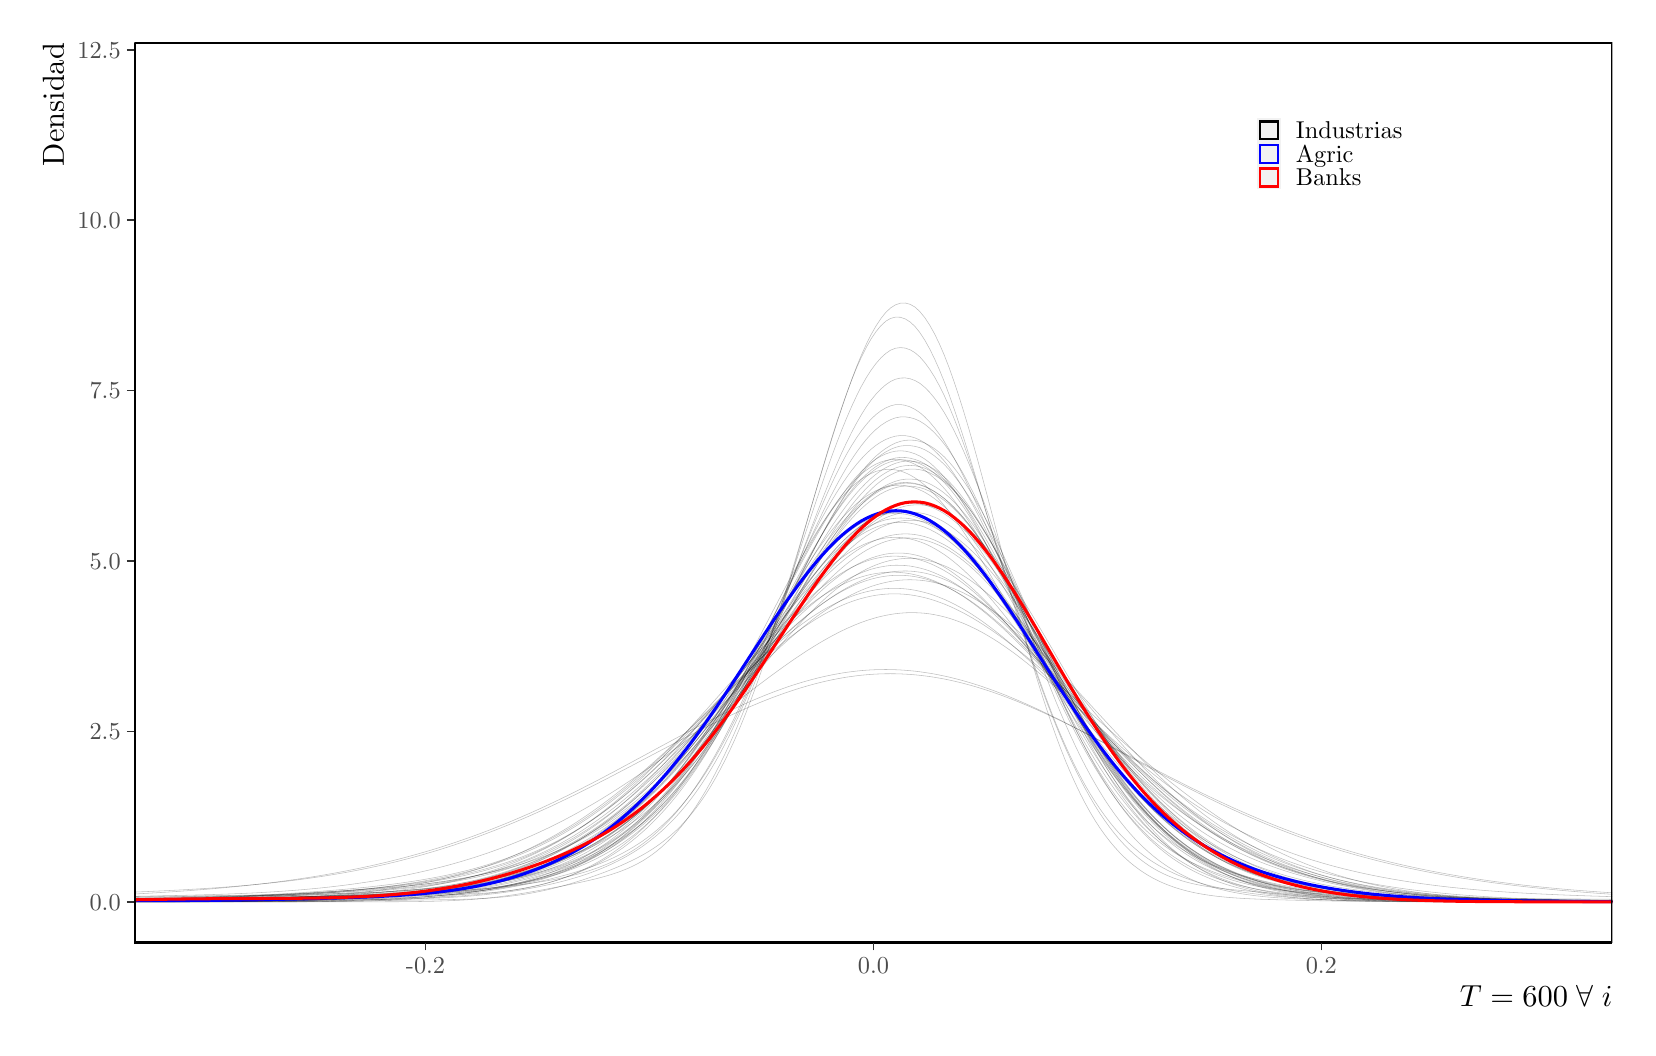
\begin{tikzpicture}[x=1pt,y=1pt]
\definecolor{fillColor}{RGB}{255,255,255}
\path[use as bounding box,fill=fillColor,fill opacity=0.00] (0,0) rectangle (578.16,361.35);
\begin{scope}
\path[clip] (  0.00,  0.00) rectangle (578.16,361.35);
\definecolor{drawColor}{RGB}{255,255,255}
\definecolor{fillColor}{RGB}{255,255,255}

\path[draw=drawColor,line width= 0.6pt,line join=round,line cap=round,fill=fillColor] (  0.00,  0.00) rectangle (578.16,361.35);
\end{scope}
\begin{scope}
\path[clip] ( 38.56, 30.69) rectangle (572.66,355.85);
\definecolor{drawColor}{RGB}{0,0,0}

\path[draw=drawColor,draw opacity=0.25,line width= 0.2pt,line join=round] (-117.55, 45.47) --
	(-115.79, 45.47) --
	(-114.03, 45.47) --
	(-112.27, 45.47) --
	(-110.51, 45.47) --
	(-108.75, 45.47) --
	(-106.99, 45.47) --
	(-105.23, 45.47) --
	(-103.47, 45.47) --
	(-101.71, 45.47) --
	(-99.95, 45.47) --
	(-98.19, 45.47) --
	(-96.43, 45.47) --
	(-94.67, 45.47) --
	(-92.91, 45.47) --
	(-91.15, 45.47) --
	(-89.39, 45.47) --
	(-87.63, 45.47) --
	(-85.87, 45.47) --
	(-84.11, 45.47) --
	(-82.35, 45.47) --
	(-80.59, 45.47) --
	(-78.83, 45.47) --
	(-77.07, 45.47) --
	(-75.31, 45.47) --
	(-73.55, 45.47) --
	(-71.79, 45.47) --
	(-70.03, 45.47) --
	(-68.28, 45.47) --
	(-66.52, 45.47) --
	(-64.76, 45.47) --
	(-63.00, 45.48) --
	(-61.24, 45.48) --
	(-59.48, 45.48) --
	(-57.72, 45.48) --
	(-55.96, 45.48) --
	(-54.20, 45.48) --
	(-52.44, 45.49) --
	(-50.68, 45.49) --
	(-48.92, 45.49) --
	(-47.16, 45.50) --
	(-45.40, 45.50) --
	(-43.64, 45.51) --
	(-41.88, 45.51) --
	(-40.12, 45.52) --
	(-38.36, 45.52) --
	(-36.60, 45.53) --
	(-34.84, 45.53) --
	(-33.08, 45.54) --
	(-31.32, 45.55) --
	(-29.56, 45.56) --
	(-27.80, 45.56) --
	(-26.04, 45.57) --
	(-24.28, 45.58) --
	(-22.52, 45.59) --
	(-20.76, 45.60) --
	(-19.00, 45.61) --
	(-17.24, 45.62) --
	(-15.48, 45.64) --
	(-13.72, 45.65) --
	(-11.96, 45.66) --
	(-10.20, 45.67) --
	( -8.44, 45.69) --
	( -6.68, 45.70) --
	( -4.92, 45.71) --
	( -3.16, 45.73) --
	( -1.41, 45.74) --
	(  0.35, 45.75) --
	(  2.11, 45.76) --
	(  3.87, 45.78) --
	(  5.63, 45.79) --
	(  7.39, 45.80) --
	(  9.15, 45.81) --
	( 10.91, 45.82) --
	( 12.67, 45.83) --
	( 14.43, 45.84) --
	( 16.19, 45.85) --
	( 17.95, 45.86) --
	( 19.71, 45.87) --
	( 21.47, 45.88) --
	( 23.23, 45.88) --
	( 24.99, 45.89) --
	( 26.75, 45.89) --
	( 28.51, 45.90) --
	( 30.27, 45.90) --
	( 32.03, 45.91) --
	( 33.79, 45.91) --
	( 35.55, 45.91) --
	( 37.31, 45.92) --
	( 39.07, 45.92) --
	( 40.83, 45.92) --
	( 42.59, 45.92) --
	( 44.35, 45.93) --
	( 46.11, 45.93) --
	( 47.87, 45.93) --
	( 49.63, 45.93) --
	( 51.39, 45.94) --
	( 53.15, 45.94) --
	( 54.91, 45.95) --
	( 56.67, 45.96) --
	( 58.43, 45.96) --
	( 60.19, 45.97) --
	( 61.95, 45.98) --
	( 63.71, 46.00) --
	( 65.46, 46.01) --
	( 67.22, 46.02) --
	( 68.98, 46.04) --
	( 70.74, 46.06) --
	( 72.50, 46.08) --
	( 74.26, 46.10) --
	( 76.02, 46.12) --
	( 77.78, 46.15) --
	( 79.54, 46.17) --
	( 81.30, 46.20) --
	( 83.06, 46.23) --
	( 84.82, 46.26) --
	( 86.58, 46.29) --
	( 88.34, 46.32) --
	( 90.10, 46.36) --
	( 91.86, 46.39) --
	( 93.62, 46.43) --
	( 95.38, 46.46) --
	( 97.14, 46.50) --
	( 98.90, 46.54) --
	(100.66, 46.58) --
	(102.42, 46.62) --
	(104.18, 46.67) --
	(105.94, 46.71) --
	(107.70, 46.76) --
	(109.46, 46.80) --
	(111.22, 46.85) --
	(112.98, 46.90) --
	(114.74, 46.96) --
	(116.50, 47.01) --
	(118.26, 47.07) --
	(120.02, 47.13) --
	(121.78, 47.20) --
	(123.54, 47.26) --
	(125.30, 47.34) --
	(127.06, 47.42) --
	(128.82, 47.50) --
	(130.58, 47.59) --
	(132.33, 47.69) --
	(134.09, 47.79) --
	(135.85, 47.91) --
	(137.61, 48.03) --
	(139.37, 48.16) --
	(141.13, 48.30) --
	(142.89, 48.45) --
	(144.65, 48.62) --
	(146.41, 48.80) --
	(148.17, 48.99) --
	(149.93, 49.19) --
	(151.69, 49.42) --
	(153.45, 49.65) --
	(155.21, 49.91) --
	(156.97, 50.18) --
	(158.73, 50.47) --
	(160.49, 50.78) --
	(162.25, 51.11) --
	(164.01, 51.47) --
	(165.77, 51.84) --
	(167.53, 52.24) --
	(169.29, 52.66) --
	(171.05, 53.11) --
	(172.81, 53.59) --
	(174.57, 54.09) --
	(176.33, 54.62) --
	(178.09, 55.18) --
	(179.85, 55.77) --
	(181.61, 56.40) --
	(183.37, 57.05) --
	(185.13, 57.74) --
	(186.89, 58.46) --
	(188.65, 59.22) --
	(190.41, 60.02) --
	(192.17, 60.85) --
	(193.93, 61.73) --
	(195.69, 62.65) --
	(197.45, 63.62) --
	(199.21, 64.62) --
	(200.96, 65.66) --
	(202.72, 66.77) --
	(204.48, 67.92) --
	(206.24, 69.12) --
	(208.00, 70.37) --
	(209.76, 71.68) --
	(211.52, 73.04) --
	(213.28, 74.46) --
	(215.04, 75.93) --
	(216.80, 77.46) --
	(218.56, 79.06) --
	(220.32, 80.71) --
	(222.08, 82.42) --
	(223.84, 84.19) --
	(225.60, 86.03) --
	(227.36, 87.94) --
	(229.12, 89.90) --
	(230.88, 91.92) --
	(232.64, 94.00) --
	(234.40, 96.15) --
	(236.16, 98.36) --
	(237.92,100.61) --
	(239.68,102.92) --
	(241.44,105.30) --
	(243.20,107.72) --
	(244.96,110.18) --
	(246.72,112.69) --
	(248.48,115.24) --
	(250.24,117.84) --
	(252.00,120.46) --
	(253.76,123.10) --
	(255.52,125.77) --
	(257.28,128.46) --
	(259.04,131.16) --
	(260.80,133.87) --
	(262.56,136.57) --
	(264.32,139.27) --
	(266.08,141.96) --
	(267.83,144.63) --
	(269.59,147.28) --
	(271.35,149.89) --
	(273.11,152.46) --
	(274.87,154.99) --
	(276.63,157.47) --
	(278.39,159.90) --
	(280.15,162.24) --
	(281.91,164.51) --
	(283.67,166.72) --
	(285.43,168.84) --
	(287.19,170.86) --
	(288.95,172.78) --
	(290.71,174.60) --
	(292.47,176.33) --
	(294.23,177.93) --
	(295.99,179.40) --
	(297.75,180.75) --
	(299.51,181.99) --
	(301.27,183.10) --
	(303.03,184.05) --
	(304.79,184.86) --
	(306.55,185.54) --
	(308.31,186.09) --
	(310.07,186.48) --
	(311.83,186.70) --
	(313.59,186.79) --
	(315.35,186.75) --
	(317.11,186.55) --
	(318.87,186.17) --
	(320.63,185.66) --
	(322.39,185.01) --
	(324.15,184.23) --
	(325.91,183.27) --
	(327.67,182.17) --
	(329.43,180.95) --
	(331.19,179.61) --
	(332.95,178.12) --
	(334.70,176.49) --
	(336.46,174.75) --
	(338.22,172.91) --
	(339.98,170.96) --
	(341.74,168.89) --
	(343.50,166.72) --
	(345.26,164.47) --
	(347.02,162.15) --
	(348.78,159.73) --
	(350.54,157.24) --
	(352.30,154.70) --
	(354.06,152.10) --
	(355.82,149.46) --
	(357.58,146.77) --
	(359.34,144.05) --
	(361.10,141.31) --
	(362.86,138.55) --
	(364.62,135.77) --
	(366.38,133.00) --
	(368.14,130.22) --
	(369.90,127.46) --
	(371.66,124.71) --
	(373.42,121.99) --
	(375.18,119.29) --
	(376.94,116.62) --
	(378.70,113.99) --
	(380.46,111.41) --
	(382.22,108.87) --
	(383.98,106.37) --
	(385.74,103.93) --
	(387.50,101.55) --
	(389.26, 99.23) --
	(391.02, 96.97) --
	(392.78, 94.76) --
	(394.54, 92.63) --
	(396.30, 90.56) --
	(398.06, 88.56) --
	(399.82, 86.62) --
	(401.57, 84.74) --
	(403.33, 82.95) --
	(405.09, 81.21) --
	(406.85, 79.54) --
	(408.61, 77.92) --
	(410.37, 76.38) --
	(412.13, 74.91) --
	(413.89, 73.49) --
	(415.65, 72.13) --
	(417.41, 70.82) --
	(419.17, 69.59) --
	(420.93, 68.40) --
	(422.69, 67.26) --
	(424.45, 66.17) --
	(426.21, 65.14) --
	(427.97, 64.16) --
	(429.73, 63.21) --
	(431.49, 62.31) --
	(433.25, 61.45) --
	(435.01, 60.64) --
	(436.77, 59.86) --
	(438.53, 59.12) --
	(440.29, 58.41) --
	(442.05, 57.74) --
	(443.81, 57.09) --
	(445.57, 56.48) --
	(447.33, 55.89) --
	(449.09, 55.34) --
	(450.85, 54.81) --
	(452.61, 54.30) --
	(454.37, 53.82) --
	(456.13, 53.36) --
	(457.89, 52.92) --
	(459.65, 52.51) --
	(461.41, 52.11) --
	(463.17, 51.73) --
	(464.93, 51.37) --
	(466.69, 51.03) --
	(468.44, 50.70) --
	(470.20, 50.39) --
	(471.96, 50.10) --
	(473.72, 49.82) --
	(475.48, 49.56) --
	(477.24, 49.31) --
	(479.00, 49.07) --
	(480.76, 48.85) --
	(482.52, 48.64) --
	(484.28, 48.43) --
	(486.04, 48.24) --
	(487.80, 48.07) --
	(489.56, 47.90) --
	(491.32, 47.75) --
	(493.08, 47.60) --
	(494.84, 47.46) --
	(496.60, 47.33) --
	(498.36, 47.21) --
	(500.12, 47.10) --
	(501.88, 46.99) --
	(503.64, 46.89) --
	(505.40, 46.80) --
	(507.16, 46.71) --
	(508.92, 46.63) --
	(510.68, 46.56) --
	(512.44, 46.49) --
	(514.20, 46.42) --
	(515.96, 46.36) --
	(517.72, 46.30) --
	(519.48, 46.25) --
	(521.24, 46.20) --
	(523.00, 46.16) --
	(524.76, 46.11) --
	(526.52, 46.07) --
	(528.28, 46.03) --
	(530.04, 46.00) --
	(531.80, 45.96) --
	(533.56, 45.93) --
	(535.32, 45.90) --
	(537.07, 45.87) --
	(538.83, 45.84) --
	(540.59, 45.82) --
	(542.35, 45.79) --
	(544.11, 45.77) --
	(545.87, 45.75) --
	(547.63, 45.73) --
	(549.39, 45.71) --
	(551.15, 45.69) --
	(552.91, 45.68) --
	(554.67, 45.66) --
	(556.43, 45.64) --
	(558.19, 45.63) --
	(559.95, 45.62) --
	(561.71, 45.60) --
	(563.47, 45.59) --
	(565.23, 45.58) --
	(566.99, 45.57) --
	(568.75, 45.56) --
	(570.51, 45.55) --
	(572.27, 45.54) --
	(574.03, 45.54) --
	(575.79, 45.53) --
	(577.55, 45.52) --
	(579.31, 45.52) --
	(581.07, 45.51) --
	(582.83, 45.51) --
	(584.59, 45.50) --
	(586.35, 45.50) --
	(588.11, 45.49) --
	(589.87, 45.49) --
	(591.63, 45.49) --
	(593.39, 45.48) --
	(595.15, 45.48) --
	(596.91, 45.48) --
	(598.67, 45.48) --
	(600.43, 45.48) --
	(602.19, 45.48) --
	(603.94, 45.47) --
	(605.70, 45.47) --
	(607.46, 45.47) --
	(609.22, 45.47) --
	(610.98, 45.47) --
	(612.74, 45.47) --
	(614.50, 45.47) --
	(616.26, 45.47) --
	(618.02, 45.47) --
	(619.78, 45.47) --
	(621.54, 45.47) --
	(623.30, 45.47) --
	(625.06, 45.47) --
	(626.82, 45.47) --
	(628.58, 45.47) --
	(630.34, 45.47) --
	(632.10, 45.47) --
	(633.86, 45.47) --
	(635.62, 45.47) --
	(637.38, 45.47) --
	(639.14, 45.47) --
	(640.90, 45.47) --
	(642.66, 45.47) --
	(644.42, 45.47) --
	(646.18, 45.47) --
	(647.94, 45.47) --
	(649.70, 45.47) --
	(651.46, 45.47) --
	(653.22, 45.47) --
	(654.98, 45.47) --
	(656.74, 45.47) --
	(658.50, 45.47) --
	(660.26, 45.47) --
	(662.02, 45.47) --
	(663.78, 45.47) --
	(665.54, 45.47) --
	(667.30, 45.47) --
	(669.06, 45.47) --
	(670.81, 45.47) --
	(672.57, 45.47) --
	(674.33, 45.47) --
	(676.09, 45.47) --
	(677.85, 45.47) --
	(679.61, 45.47) --
	(681.37, 45.47) --
	(683.13, 45.47) --
	(684.89, 45.47) --
	(686.65, 45.47) --
	(688.41, 45.47) --
	(690.17, 45.47) --
	(691.93, 45.47) --
	(693.69, 45.47) --
	(695.45, 45.47) --
	(697.21, 45.47) --
	(698.97, 45.47) --
	(700.73, 45.47) --
	(702.49, 45.47) --
	(704.25, 45.47) --
	(706.01, 45.47) --
	(707.77, 45.47) --
	(709.53, 45.47) --
	(711.29, 45.47) --
	(713.05, 45.47) --
	(714.81, 45.47) --
	(716.57, 45.47) --
	(718.33, 45.47) --
	(720.09, 45.47) --
	(721.85, 45.47) --
	(723.61, 45.47) --
	(725.37, 45.47) --
	(727.13, 45.47) --
	(728.89, 45.47) --
	(730.65, 45.47) --
	(732.41, 45.47) --
	(734.17, 45.47) --
	(735.93, 45.47) --
	(737.68, 45.47) --
	(739.44, 45.47) --
	(741.20, 45.47) --
	(742.96, 45.47) --
	(744.72, 45.47) --
	(746.48, 45.47) --
	(748.24, 45.47) --
	(750.00, 45.47) --
	(751.76, 45.47) --
	(753.52, 45.47) --
	(755.28, 45.47) --
	(757.04, 45.47) --
	(758.80, 45.47) --
	(760.56, 45.47) --
	(762.32, 45.47) --
	(764.08, 45.47) --
	(765.84, 45.47) --
	(767.60, 45.47) --
	(769.36, 45.47) --
	(771.12, 45.47) --
	(772.88, 45.47) --
	(774.64, 45.47) --
	(776.40, 45.47) --
	(778.16, 45.47) --
	(779.92, 45.47) --
	(781.68, 45.47);

\path[draw=drawColor,draw opacity=0.25,line width= 0.2pt,line join=round] (-117.55, 45.47) --
	(-115.79, 45.47) --
	(-114.03, 45.47) --
	(-112.27, 45.47) --
	(-110.51, 45.47) --
	(-108.75, 45.47) --
	(-106.99, 45.47) --
	(-105.23, 45.47) --
	(-103.47, 45.47) --
	(-101.71, 45.47) --
	(-99.95, 45.47) --
	(-98.19, 45.47) --
	(-96.43, 45.47) --
	(-94.67, 45.47) --
	(-92.91, 45.47) --
	(-91.15, 45.47) --
	(-89.39, 45.47) --
	(-87.63, 45.47) --
	(-85.87, 45.47) --
	(-84.11, 45.47) --
	(-82.35, 45.47) --
	(-80.59, 45.47) --
	(-78.83, 45.47) --
	(-77.07, 45.47) --
	(-75.31, 45.47) --
	(-73.55, 45.47) --
	(-71.79, 45.47) --
	(-70.03, 45.47) --
	(-68.28, 45.47) --
	(-66.52, 45.47) --
	(-64.76, 45.47) --
	(-63.00, 45.47) --
	(-61.24, 45.47) --
	(-59.48, 45.47) --
	(-57.72, 45.47) --
	(-55.96, 45.47) --
	(-54.20, 45.47) --
	(-52.44, 45.47) --
	(-50.68, 45.47) --
	(-48.92, 45.47) --
	(-47.16, 45.47) --
	(-45.40, 45.47) --
	(-43.64, 45.47) --
	(-41.88, 45.47) --
	(-40.12, 45.47) --
	(-38.36, 45.47) --
	(-36.60, 45.47) --
	(-34.84, 45.47) --
	(-33.08, 45.47) --
	(-31.32, 45.47) --
	(-29.56, 45.47) --
	(-27.80, 45.47) --
	(-26.04, 45.47) --
	(-24.28, 45.47) --
	(-22.52, 45.47) --
	(-20.76, 45.47) --
	(-19.00, 45.47) --
	(-17.24, 45.47) --
	(-15.48, 45.47) --
	(-13.72, 45.47) --
	(-11.96, 45.47) --
	(-10.20, 45.47) --
	( -8.44, 45.47) --
	( -6.68, 45.47) --
	( -4.92, 45.47) --
	( -3.16, 45.47) --
	( -1.41, 45.47) --
	(  0.35, 45.47) --
	(  2.11, 45.47) --
	(  3.87, 45.47) --
	(  5.63, 45.47) --
	(  7.39, 45.47) --
	(  9.15, 45.47) --
	( 10.91, 45.47) --
	( 12.67, 45.47) --
	( 14.43, 45.47) --
	( 16.19, 45.47) --
	( 17.95, 45.47) --
	( 19.71, 45.47) --
	( 21.47, 45.47) --
	( 23.23, 45.47) --
	( 24.99, 45.47) --
	( 26.75, 45.47) --
	( 28.51, 45.47) --
	( 30.27, 45.47) --
	( 32.03, 45.47) --
	( 33.79, 45.47) --
	( 35.55, 45.47) --
	( 37.31, 45.47) --
	( 39.07, 45.47) --
	( 40.83, 45.47) --
	( 42.59, 45.47) --
	( 44.35, 45.47) --
	( 46.11, 45.47) --
	( 47.87, 45.47) --
	( 49.63, 45.47) --
	( 51.39, 45.47) --
	( 53.15, 45.47) --
	( 54.91, 45.47) --
	( 56.67, 45.47) --
	( 58.43, 45.47) --
	( 60.19, 45.47) --
	( 61.95, 45.47) --
	( 63.71, 45.47) --
	( 65.46, 45.47) --
	( 67.22, 45.47) --
	( 68.98, 45.47) --
	( 70.74, 45.47) --
	( 72.50, 45.47) --
	( 74.26, 45.47) --
	( 76.02, 45.47) --
	( 77.78, 45.47) --
	( 79.54, 45.47) --
	( 81.30, 45.47) --
	( 83.06, 45.48) --
	( 84.82, 45.48) --
	( 86.58, 45.48) --
	( 88.34, 45.48) --
	( 90.10, 45.49) --
	( 91.86, 45.49) --
	( 93.62, 45.50) --
	( 95.38, 45.51) --
	( 97.14, 45.51) --
	( 98.90, 45.52) --
	(100.66, 45.53) --
	(102.42, 45.55) --
	(104.18, 45.56) --
	(105.94, 45.58) --
	(107.70, 45.59) --
	(109.46, 45.61) --
	(111.22, 45.63) --
	(112.98, 45.66) --
	(114.74, 45.68) --
	(116.50, 45.71) --
	(118.26, 45.73) --
	(120.02, 45.76) --
	(121.78, 45.79) --
	(123.54, 45.82) --
	(125.30, 45.85) --
	(127.06, 45.88) --
	(128.82, 45.92) --
	(130.58, 45.95) --
	(132.33, 45.98) --
	(134.09, 46.01) --
	(135.85, 46.03) --
	(137.61, 46.06) --
	(139.37, 46.09) --
	(141.13, 46.11) --
	(142.89, 46.14) --
	(144.65, 46.16) --
	(146.41, 46.19) --
	(148.17, 46.21) --
	(149.93, 46.24) --
	(151.69, 46.27) --
	(153.45, 46.30) --
	(155.21, 46.34) --
	(156.97, 46.38) --
	(158.73, 46.43) --
	(160.49, 46.49) --
	(162.25, 46.56) --
	(164.01, 46.65) --
	(165.77, 46.75) --
	(167.53, 46.86) --
	(169.29, 47.00) --
	(171.05, 47.15) --
	(172.81, 47.33) --
	(174.57, 47.53) --
	(176.33, 47.75) --
	(178.09, 47.99) --
	(179.85, 48.26) --
	(181.61, 48.56) --
	(183.37, 48.89) --
	(185.13, 49.24) --
	(186.89, 49.62) --
	(188.65, 50.03) --
	(190.41, 50.45) --
	(192.17, 50.91) --
	(193.93, 51.39) --
	(195.69, 51.89) --
	(197.45, 52.41) --
	(199.21, 52.96) --
	(200.96, 53.52) --
	(202.72, 54.11) --
	(204.48, 54.72) --
	(206.24, 55.35) --
	(208.00, 56.00) --
	(209.76, 56.67) --
	(211.52, 57.37) --
	(213.28, 58.09) --
	(215.04, 58.86) --
	(216.80, 59.66) --
	(218.56, 60.50) --
	(220.32, 61.39) --
	(222.08, 62.33) --
	(223.84, 63.34) --
	(225.60, 64.43) --
	(227.36, 65.61) --
	(229.12, 66.88) --
	(230.88, 68.25) --
	(232.64, 69.73) --
	(234.40, 71.32) --
	(236.16, 73.08) --
	(237.92, 74.99) --
	(239.68, 77.05) --
	(241.44, 79.28) --
	(243.20, 81.68) --
	(244.96, 84.25) --
	(246.72, 87.05) --
	(248.48, 90.06) --
	(250.24, 93.27) --
	(252.00, 96.68) --
	(253.76,100.30) --
	(255.52,104.13) --
	(257.28,108.20) --
	(259.04,112.50) --
	(260.80,117.00) --
	(262.56,121.71) --
	(264.32,126.61) --
	(266.08,131.70) --
	(267.83,136.98) --
	(269.59,142.45) --
	(271.35,148.07) --
	(273.11,153.82) --
	(274.87,159.68) --
	(276.63,165.65) --
	(278.39,171.69) --
	(280.15,177.79) --
	(281.91,183.90) --
	(283.67,189.99) --
	(285.43,196.04) --
	(287.19,202.02) --
	(288.95,207.89) --
	(290.71,213.58) --
	(292.47,219.07) --
	(294.23,224.33) --
	(295.99,229.33) --
	(297.75,234.04) --
	(299.51,238.41) --
	(301.27,242.33) --
	(303.03,245.84) --
	(304.79,248.91) --
	(306.55,251.52) --
	(308.31,253.65) --
	(310.07,255.28) --
	(311.83,256.29) --
	(313.59,256.76) --
	(315.35,256.70) --
	(317.11,256.11) --
	(318.87,255.00) --
	(320.63,253.38) --
	(322.39,251.18) --
	(324.15,248.47) --
	(325.91,245.32) --
	(327.67,241.74) --
	(329.43,237.78) --
	(331.19,233.45) --
	(332.95,228.76) --
	(334.70,223.76) --
	(336.46,218.51) --
	(338.22,213.06) --
	(339.98,207.44) --
	(341.74,201.69) --
	(343.50,195.82) --
	(345.26,189.88) --
	(347.02,183.91) --
	(348.78,177.94) --
	(350.54,171.99) --
	(352.30,166.08) --
	(354.06,160.24) --
	(355.82,154.50) --
	(357.58,148.87) --
	(359.34,143.36) --
	(361.10,137.98) --
	(362.86,132.73) --
	(364.62,127.63) --
	(366.38,122.71) --
	(368.14,117.96) --
	(369.90,113.37) --
	(371.66,108.96) --
	(373.42,104.71) --
	(375.18,100.63) --
	(376.94, 96.77) --
	(378.70, 93.08) --
	(380.46, 89.58) --
	(382.22, 86.25) --
	(383.98, 83.10) --
	(385.74, 80.12) --
	(387.50, 77.35) --
	(389.26, 74.76) --
	(391.02, 72.33) --
	(392.78, 70.08) --
	(394.54, 67.98) --
	(396.30, 66.04) --
	(398.06, 64.27) --
	(399.82, 62.66) --
	(401.57, 61.18) --
	(403.33, 59.84) --
	(405.09, 58.62) --
	(406.85, 57.51) --
	(408.61, 56.52) --
	(410.37, 55.64) --
	(412.13, 54.86) --
	(413.89, 54.15) --
	(415.65, 53.53) --
	(417.41, 52.97) --
	(419.17, 52.48) --
	(420.93, 52.05) --
	(422.69, 51.67) --
	(424.45, 51.33) --
	(426.21, 51.03) --
	(427.97, 50.76) --
	(429.73, 50.52) --
	(431.49, 50.30) --
	(433.25, 50.10) --
	(435.01, 49.91) --
	(436.77, 49.74) --
	(438.53, 49.57) --
	(440.29, 49.41) --
	(442.05, 49.25) --
	(443.81, 49.10) --
	(445.57, 48.94) --
	(447.33, 48.79) --
	(449.09, 48.63) --
	(450.85, 48.48) --
	(452.61, 48.32) --
	(454.37, 48.16) --
	(456.13, 48.00) --
	(457.89, 47.84) --
	(459.65, 47.68) --
	(461.41, 47.53) --
	(463.17, 47.37) --
	(464.93, 47.22) --
	(466.69, 47.08) --
	(468.44, 46.93) --
	(470.20, 46.80) --
	(471.96, 46.67) --
	(473.72, 46.54) --
	(475.48, 46.43) --
	(477.24, 46.32) --
	(479.00, 46.22) --
	(480.76, 46.13) --
	(482.52, 46.04) --
	(484.28, 45.97) --
	(486.04, 45.90) --
	(487.80, 45.84) --
	(489.56, 45.78) --
	(491.32, 45.74) --
	(493.08, 45.69) --
	(494.84, 45.66) --
	(496.60, 45.62) --
	(498.36, 45.60) --
	(500.12, 45.57) --
	(501.88, 45.55) --
	(503.64, 45.54) --
	(505.40, 45.52) --
	(507.16, 45.51) --
	(508.92, 45.50) --
	(510.68, 45.50) --
	(512.44, 45.49) --
	(514.20, 45.48) --
	(515.96, 45.48) --
	(517.72, 45.48) --
	(519.48, 45.47) --
	(521.24, 45.47) --
	(523.00, 45.47) --
	(524.76, 45.47) --
	(526.52, 45.47) --
	(528.28, 45.47) --
	(530.04, 45.47) --
	(531.80, 45.47) --
	(533.56, 45.47) --
	(535.32, 45.47) --
	(537.07, 45.47) --
	(538.83, 45.47) --
	(540.59, 45.47) --
	(542.35, 45.47) --
	(544.11, 45.47) --
	(545.87, 45.47) --
	(547.63, 45.47) --
	(549.39, 45.47) --
	(551.15, 45.47) --
	(552.91, 45.47) --
	(554.67, 45.47) --
	(556.43, 45.47) --
	(558.19, 45.47) --
	(559.95, 45.47) --
	(561.71, 45.47) --
	(563.47, 45.47) --
	(565.23, 45.47) --
	(566.99, 45.47) --
	(568.75, 45.47) --
	(570.51, 45.47) --
	(572.27, 45.47) --
	(574.03, 45.47) --
	(575.79, 45.47) --
	(577.55, 45.47) --
	(579.31, 45.47) --
	(581.07, 45.47) --
	(582.83, 45.47) --
	(584.59, 45.47) --
	(586.35, 45.47) --
	(588.11, 45.47) --
	(589.87, 45.47) --
	(591.63, 45.47) --
	(593.39, 45.47) --
	(595.15, 45.47) --
	(596.91, 45.47) --
	(598.67, 45.47) --
	(600.43, 45.47) --
	(602.19, 45.47) --
	(603.94, 45.47) --
	(605.70, 45.47) --
	(607.46, 45.47) --
	(609.22, 45.47) --
	(610.98, 45.47) --
	(612.74, 45.47) --
	(614.50, 45.47) --
	(616.26, 45.47) --
	(618.02, 45.47) --
	(619.78, 45.47) --
	(621.54, 45.47) --
	(623.30, 45.47) --
	(625.06, 45.47) --
	(626.82, 45.47) --
	(628.58, 45.47) --
	(630.34, 45.47) --
	(632.10, 45.47) --
	(633.86, 45.47) --
	(635.62, 45.47) --
	(637.38, 45.47) --
	(639.14, 45.47) --
	(640.90, 45.47) --
	(642.66, 45.47) --
	(644.42, 45.47) --
	(646.18, 45.47) --
	(647.94, 45.47) --
	(649.70, 45.47) --
	(651.46, 45.47) --
	(653.22, 45.47) --
	(654.98, 45.47) --
	(656.74, 45.47) --
	(658.50, 45.47) --
	(660.26, 45.47) --
	(662.02, 45.47) --
	(663.78, 45.47) --
	(665.54, 45.47) --
	(667.30, 45.47) --
	(669.06, 45.47) --
	(670.81, 45.47) --
	(672.57, 45.47) --
	(674.33, 45.47) --
	(676.09, 45.47) --
	(677.85, 45.47) --
	(679.61, 45.47) --
	(681.37, 45.47) --
	(683.13, 45.47) --
	(684.89, 45.47) --
	(686.65, 45.47) --
	(688.41, 45.47) --
	(690.17, 45.47) --
	(691.93, 45.47) --
	(693.69, 45.47) --
	(695.45, 45.47) --
	(697.21, 45.47) --
	(698.97, 45.47) --
	(700.73, 45.47) --
	(702.49, 45.47) --
	(704.25, 45.47) --
	(706.01, 45.47) --
	(707.77, 45.47) --
	(709.53, 45.47) --
	(711.29, 45.47) --
	(713.05, 45.47) --
	(714.81, 45.47) --
	(716.57, 45.47) --
	(718.33, 45.47) --
	(720.09, 45.47) --
	(721.85, 45.47) --
	(723.61, 45.47) --
	(725.37, 45.47) --
	(727.13, 45.47) --
	(728.89, 45.47) --
	(730.65, 45.47) --
	(732.41, 45.47) --
	(734.17, 45.47) --
	(735.93, 45.47) --
	(737.68, 45.47) --
	(739.44, 45.47) --
	(741.20, 45.47) --
	(742.96, 45.47) --
	(744.72, 45.47) --
	(746.48, 45.47) --
	(748.24, 45.47) --
	(750.00, 45.47) --
	(751.76, 45.47) --
	(753.52, 45.47) --
	(755.28, 45.47) --
	(757.04, 45.47) --
	(758.80, 45.47) --
	(760.56, 45.47) --
	(762.32, 45.47) --
	(764.08, 45.47) --
	(765.84, 45.47) --
	(767.60, 45.47) --
	(769.36, 45.47) --
	(771.12, 45.47) --
	(772.88, 45.47) --
	(774.64, 45.47) --
	(776.40, 45.47) --
	(778.16, 45.47) --
	(779.92, 45.47) --
	(781.68, 45.47);

\path[draw=drawColor,draw opacity=0.25,line width= 0.2pt,line join=round] (-117.55, 45.47) --
	(-115.79, 45.47) --
	(-114.03, 45.47) --
	(-112.27, 45.47) --
	(-110.51, 45.47) --
	(-108.75, 45.47) --
	(-106.99, 45.47) --
	(-105.23, 45.47) --
	(-103.47, 45.47) --
	(-101.71, 45.47) --
	(-99.95, 45.47) --
	(-98.19, 45.47) --
	(-96.43, 45.47) --
	(-94.67, 45.47) --
	(-92.91, 45.47) --
	(-91.15, 45.47) --
	(-89.39, 45.47) --
	(-87.63, 45.47) --
	(-85.87, 45.47) --
	(-84.11, 45.47) --
	(-82.35, 45.47) --
	(-80.59, 45.47) --
	(-78.83, 45.47) --
	(-77.07, 45.47) --
	(-75.31, 45.47) --
	(-73.55, 45.47) --
	(-71.79, 45.47) --
	(-70.03, 45.47) --
	(-68.28, 45.47) --
	(-66.52, 45.47) --
	(-64.76, 45.47) --
	(-63.00, 45.47) --
	(-61.24, 45.47) --
	(-59.48, 45.47) --
	(-57.72, 45.47) --
	(-55.96, 45.47) --
	(-54.20, 45.47) --
	(-52.44, 45.47) --
	(-50.68, 45.47) --
	(-48.92, 45.47) --
	(-47.16, 45.47) --
	(-45.40, 45.47) --
	(-43.64, 45.47) --
	(-41.88, 45.47) --
	(-40.12, 45.47) --
	(-38.36, 45.47) --
	(-36.60, 45.47) --
	(-34.84, 45.47) --
	(-33.08, 45.47) --
	(-31.32, 45.48) --
	(-29.56, 45.48) --
	(-27.80, 45.48) --
	(-26.04, 45.48) --
	(-24.28, 45.49) --
	(-22.52, 45.49) --
	(-20.76, 45.49) --
	(-19.00, 45.50) --
	(-17.24, 45.50) --
	(-15.48, 45.51) --
	(-13.72, 45.51) --
	(-11.96, 45.52) --
	(-10.20, 45.53) --
	( -8.44, 45.54) --
	( -6.68, 45.55) --
	( -4.92, 45.56) --
	( -3.16, 45.57) --
	( -1.41, 45.58) --
	(  0.35, 45.59) --
	(  2.11, 45.61) --
	(  3.87, 45.63) --
	(  5.63, 45.64) --
	(  7.39, 45.66) --
	(  9.15, 45.68) --
	( 10.91, 45.71) --
	( 12.67, 45.73) --
	( 14.43, 45.75) --
	( 16.19, 45.78) --
	( 17.95, 45.81) --
	( 19.71, 45.84) --
	( 21.47, 45.87) --
	( 23.23, 45.90) --
	( 24.99, 45.93) --
	( 26.75, 45.96) --
	( 28.51, 46.00) --
	( 30.27, 46.03) --
	( 32.03, 46.07) --
	( 33.79, 46.10) --
	( 35.55, 46.14) --
	( 37.31, 46.18) --
	( 39.07, 46.22) --
	( 40.83, 46.25) --
	( 42.59, 46.29) --
	( 44.35, 46.32) --
	( 46.11, 46.36) --
	( 47.87, 46.40) --
	( 49.63, 46.43) --
	( 51.39, 46.46) --
	( 53.15, 46.50) --
	( 54.91, 46.53) --
	( 56.67, 46.56) --
	( 58.43, 46.59) --
	( 60.19, 46.62) --
	( 61.95, 46.64) --
	( 63.71, 46.67) --
	( 65.46, 46.70) --
	( 67.22, 46.72) --
	( 68.98, 46.74) --
	( 70.74, 46.77) --
	( 72.50, 46.79) --
	( 74.26, 46.81) --
	( 76.02, 46.83) --
	( 77.78, 46.85) --
	( 79.54, 46.88) --
	( 81.30, 46.90) --
	( 83.06, 46.92) --
	( 84.82, 46.94) --
	( 86.58, 46.96) --
	( 88.34, 46.99) --
	( 90.10, 47.01) --
	( 91.86, 47.04) --
	( 93.62, 47.07) --
	( 95.38, 47.10) --
	( 97.14, 47.13) --
	( 98.90, 47.16) --
	(100.66, 47.20) --
	(102.42, 47.24) --
	(104.18, 47.28) --
	(105.94, 47.32) --
	(107.70, 47.37) --
	(109.46, 47.42) --
	(111.22, 47.47) --
	(112.98, 47.53) --
	(114.74, 47.60) --
	(116.50, 47.67) --
	(118.26, 47.74) --
	(120.02, 47.82) --
	(121.78, 47.91) --
	(123.54, 48.00) --
	(125.30, 48.10) --
	(127.06, 48.21) --
	(128.82, 48.32) --
	(130.58, 48.45) --
	(132.33, 48.58) --
	(134.09, 48.72) --
	(135.85, 48.87) --
	(137.61, 49.03) --
	(139.37, 49.20) --
	(141.13, 49.38) --
	(142.89, 49.57) --
	(144.65, 49.77) --
	(146.41, 49.98) --
	(148.17, 50.21) --
	(149.93, 50.44) --
	(151.69, 50.69) --
	(153.45, 50.95) --
	(155.21, 51.22) --
	(156.97, 51.51) --
	(158.73, 51.81) --
	(160.49, 52.12) --
	(162.25, 52.44) --
	(164.01, 52.78) --
	(165.77, 53.13) --
	(167.53, 53.50) --
	(169.29, 53.88) --
	(171.05, 54.27) --
	(172.81, 54.68) --
	(174.57, 55.11) --
	(176.33, 55.55) --
	(178.09, 56.01) --
	(179.85, 56.49) --
	(181.61, 56.99) --
	(183.37, 57.50) --
	(185.13, 58.04) --
	(186.89, 58.60) --
	(188.65, 59.18) --
	(190.41, 59.79) --
	(192.17, 60.41) --
	(193.93, 61.07) --
	(195.69, 61.76) --
	(197.45, 62.48) --
	(199.21, 63.23) --
	(200.96, 64.01) --
	(202.72, 64.83) --
	(204.48, 65.69) --
	(206.24, 66.59) --
	(208.00, 67.52) --
	(209.76, 68.50) --
	(211.52, 69.54) --
	(213.28, 70.62) --
	(215.04, 71.75) --
	(216.80, 72.93) --
	(218.56, 74.17) --
	(220.32, 75.47) --
	(222.08, 76.83) --
	(223.84, 78.25) --
	(225.60, 79.73) --
	(227.36, 81.29) --
	(229.12, 82.92) --
	(230.88, 84.61) --
	(232.64, 86.37) --
	(234.40, 88.21) --
	(236.16, 90.14) --
	(237.92, 92.14) --
	(239.68, 94.22) --
	(241.44, 96.36) --
	(243.20, 98.60) --
	(244.96,100.92) --
	(246.72,103.31) --
	(248.48,105.77) --
	(250.24,108.30) --
	(252.00,110.92) --
	(253.76,113.61) --
	(255.52,116.36) --
	(257.28,119.17) --
	(259.04,122.04) --
	(260.80,124.97) --
	(262.56,127.94) --
	(264.32,130.96) --
	(266.08,134.00) --
	(267.83,137.09) --
	(269.59,140.19) --
	(271.35,143.30) --
	(273.11,146.41) --
	(274.87,149.53) --
	(276.63,152.62) --
	(278.39,155.69) --
	(280.15,158.73) --
	(281.91,161.73) --
	(283.67,164.68) --
	(285.43,167.55) --
	(287.19,170.35) --
	(288.95,173.08) --
	(290.71,175.72) --
	(292.47,178.24) --
	(294.23,180.65) --
	(295.99,182.94) --
	(297.75,185.11) --
	(299.51,187.15) --
	(301.27,189.00) --
	(303.03,190.72) --
	(304.79,192.28) --
	(306.55,193.69) --
	(308.31,194.90) --
	(310.07,195.92) --
	(311.83,196.77) --
	(313.59,197.44) --
	(315.35,197.93) --
	(317.11,198.18) --
	(318.87,198.24) --
	(320.63,198.11) --
	(322.39,197.80) --
	(324.15,197.29) --
	(325.91,196.54) --
	(327.67,195.60) --
	(329.43,194.49) --
	(331.19,193.19) --
	(332.95,191.69) --
	(334.70,189.99) --
	(336.46,188.12) --
	(338.22,186.09) --
	(339.98,183.91) --
	(341.74,181.54) --
	(343.50,179.02) --
	(345.26,176.38) --
	(347.02,173.61) --
	(348.78,170.72) --
	(350.54,167.71) --
	(352.30,164.60) --
	(354.06,161.41) --
	(355.82,158.16) --
	(357.58,154.83) --
	(359.34,151.44) --
	(361.10,148.02) --
	(362.86,144.58) --
	(364.62,141.12) --
	(366.38,137.65) --
	(368.14,134.19) --
	(369.90,130.74) --
	(371.66,127.32) --
	(373.42,123.94) --
	(375.18,120.61) --
	(376.94,117.33) --
	(378.70,114.10) --
	(380.46,110.94) --
	(382.22,107.87) --
	(383.98,104.88) --
	(385.74,101.96) --
	(387.50, 99.13) --
	(389.26, 96.39) --
	(391.02, 93.76) --
	(392.78, 91.22) --
	(394.54, 88.78) --
	(396.30, 86.42) --
	(398.06, 84.16) --
	(399.82, 82.02) --
	(401.57, 79.96) --
	(403.33, 78.00) --
	(405.09, 76.12) --
	(406.85, 74.34) --
	(408.61, 72.65) --
	(410.37, 71.05) --
	(412.13, 69.52) --
	(413.89, 68.07) --
	(415.65, 66.71) --
	(417.41, 65.42) --
	(419.17, 64.20) --
	(420.93, 63.04) --
	(422.69, 61.94) --
	(424.45, 60.92) --
	(426.21, 59.96) --
	(427.97, 59.04) --
	(429.73, 58.18) --
	(431.49, 57.38) --
	(433.25, 56.62) --
	(435.01, 55.92) --
	(436.77, 55.25) --
	(438.53, 54.62) --
	(440.29, 54.04) --
	(442.05, 53.50) --
	(443.81, 52.99) --
	(445.57, 52.51) --
	(447.33, 52.07) --
	(449.09, 51.67) --
	(450.85, 51.29) --
	(452.61, 50.94) --
	(454.37, 50.61) --
	(456.13, 50.32) --
	(457.89, 50.04) --
	(459.65, 49.79) --
	(461.41, 49.56) --
	(463.17, 49.35) --
	(464.93, 49.16) --
	(466.69, 48.98) --
	(468.44, 48.82) --
	(470.20, 48.68) --
	(471.96, 48.55) --
	(473.72, 48.43) --
	(475.48, 48.32) --
	(477.24, 48.22) --
	(479.00, 48.13) --
	(480.76, 48.05) --
	(482.52, 47.97) --
	(484.28, 47.90) --
	(486.04, 47.84) --
	(487.80, 47.78) --
	(489.56, 47.72) --
	(491.32, 47.67) --
	(493.08, 47.61) --
	(494.84, 47.56) --
	(496.60, 47.51) --
	(498.36, 47.47) --
	(500.12, 47.42) --
	(501.88, 47.37) --
	(503.64, 47.32) --
	(505.40, 47.28) --
	(507.16, 47.23) --
	(508.92, 47.18) --
	(510.68, 47.13) --
	(512.44, 47.08) --
	(514.20, 47.03) --
	(515.96, 46.98) --
	(517.72, 46.94) --
	(519.48, 46.89) --
	(521.24, 46.84) --
	(523.00, 46.79) --
	(524.76, 46.74) --
	(526.52, 46.70) --
	(528.28, 46.65) --
	(530.04, 46.61) --
	(531.80, 46.57) --
	(533.56, 46.53) --
	(535.32, 46.49) --
	(537.07, 46.45) --
	(538.83, 46.41) --
	(540.59, 46.38) --
	(542.35, 46.35) --
	(544.11, 46.32) --
	(545.87, 46.29) --
	(547.63, 46.26) --
	(549.39, 46.23) --
	(551.15, 46.21) --
	(552.91, 46.19) --
	(554.67, 46.16) --
	(556.43, 46.14) --
	(558.19, 46.12) --
	(559.95, 46.11) --
	(561.71, 46.09) --
	(563.47, 46.07) --
	(565.23, 46.05) --
	(566.99, 46.04) --
	(568.75, 46.02) --
	(570.51, 46.00) --
	(572.27, 45.99) --
	(574.03, 45.97) --
	(575.79, 45.96) --
	(577.55, 45.94) --
	(579.31, 45.92) --
	(581.07, 45.91) --
	(582.83, 45.89) --
	(584.59, 45.87) --
	(586.35, 45.86) --
	(588.11, 45.84) --
	(589.87, 45.82) --
	(591.63, 45.80) --
	(593.39, 45.79) --
	(595.15, 45.77) --
	(596.91, 45.75) --
	(598.67, 45.74) --
	(600.43, 45.72) --
	(602.19, 45.70) --
	(603.94, 45.69) --
	(605.70, 45.67) --
	(607.46, 45.66) --
	(609.22, 45.64) --
	(610.98, 45.63) --
	(612.74, 45.62) --
	(614.50, 45.60) --
	(616.26, 45.59) --
	(618.02, 45.58) --
	(619.78, 45.57) --
	(621.54, 45.56) --
	(623.30, 45.55) --
	(625.06, 45.54) --
	(626.82, 45.54) --
	(628.58, 45.53) --
	(630.34, 45.52) --
	(632.10, 45.52) --
	(633.86, 45.51) --
	(635.62, 45.50) --
	(637.38, 45.50) --
	(639.14, 45.50) --
	(640.90, 45.49) --
	(642.66, 45.49) --
	(644.42, 45.49) --
	(646.18, 45.48) --
	(647.94, 45.48) --
	(649.70, 45.48) --
	(651.46, 45.48) --
	(653.22, 45.48) --
	(654.98, 45.47) --
	(656.74, 45.47) --
	(658.50, 45.47) --
	(660.26, 45.47) --
	(662.02, 45.47) --
	(663.78, 45.47) --
	(665.54, 45.47) --
	(667.30, 45.47) --
	(669.06, 45.47) --
	(670.81, 45.47) --
	(672.57, 45.47) --
	(674.33, 45.47) --
	(676.09, 45.47) --
	(677.85, 45.47) --
	(679.61, 45.47) --
	(681.37, 45.47) --
	(683.13, 45.47) --
	(684.89, 45.47) --
	(686.65, 45.47) --
	(688.41, 45.47) --
	(690.17, 45.47) --
	(691.93, 45.47) --
	(693.69, 45.47) --
	(695.45, 45.47) --
	(697.21, 45.47) --
	(698.97, 45.47) --
	(700.73, 45.47) --
	(702.49, 45.47) --
	(704.25, 45.47) --
	(706.01, 45.47) --
	(707.77, 45.47) --
	(709.53, 45.47) --
	(711.29, 45.47) --
	(713.05, 45.47) --
	(714.81, 45.47) --
	(716.57, 45.47) --
	(718.33, 45.47) --
	(720.09, 45.47) --
	(721.85, 45.47) --
	(723.61, 45.47) --
	(725.37, 45.47) --
	(727.13, 45.47) --
	(728.89, 45.47) --
	(730.65, 45.47) --
	(732.41, 45.47) --
	(734.17, 45.47) --
	(735.93, 45.47) --
	(737.68, 45.47) --
	(739.44, 45.47) --
	(741.20, 45.47) --
	(742.96, 45.47) --
	(744.72, 45.47) --
	(746.48, 45.47) --
	(748.24, 45.47) --
	(750.00, 45.47) --
	(751.76, 45.47) --
	(753.52, 45.47) --
	(755.28, 45.47) --
	(757.04, 45.47) --
	(758.80, 45.47) --
	(760.56, 45.47) --
	(762.32, 45.47) --
	(764.08, 45.47) --
	(765.84, 45.47) --
	(767.60, 45.47) --
	(769.36, 45.47) --
	(771.12, 45.47) --
	(772.88, 45.47) --
	(774.64, 45.47) --
	(776.40, 45.47) --
	(778.16, 45.47) --
	(779.92, 45.47) --
	(781.68, 45.47);

\path[draw=drawColor,draw opacity=0.25,line width= 0.2pt,line join=round] (-117.55, 45.47) --
	(-115.79, 45.47) --
	(-114.03, 45.47) --
	(-112.27, 45.47) --
	(-110.51, 45.47) --
	(-108.75, 45.47) --
	(-106.99, 45.47) --
	(-105.23, 45.47) --
	(-103.47, 45.47) --
	(-101.71, 45.47) --
	(-99.95, 45.47) --
	(-98.19, 45.47) --
	(-96.43, 45.47) --
	(-94.67, 45.47) --
	(-92.91, 45.47) --
	(-91.15, 45.47) --
	(-89.39, 45.47) --
	(-87.63, 45.47) --
	(-85.87, 45.47) --
	(-84.11, 45.47) --
	(-82.35, 45.47) --
	(-80.59, 45.47) --
	(-78.83, 45.47) --
	(-77.07, 45.47) --
	(-75.31, 45.47) --
	(-73.55, 45.47) --
	(-71.79, 45.47) --
	(-70.03, 45.47) --
	(-68.28, 45.47) --
	(-66.52, 45.47) --
	(-64.76, 45.47) --
	(-63.00, 45.47) --
	(-61.24, 45.47) --
	(-59.48, 45.47) --
	(-57.72, 45.47) --
	(-55.96, 45.47) --
	(-54.20, 45.47) --
	(-52.44, 45.47) --
	(-50.68, 45.47) --
	(-48.92, 45.47) --
	(-47.16, 45.47) --
	(-45.40, 45.47) --
	(-43.64, 45.47) --
	(-41.88, 45.47) --
	(-40.12, 45.47) --
	(-38.36, 45.47) --
	(-36.60, 45.47) --
	(-34.84, 45.47) --
	(-33.08, 45.47) --
	(-31.32, 45.47) --
	(-29.56, 45.47) --
	(-27.80, 45.47) --
	(-26.04, 45.47) --
	(-24.28, 45.47) --
	(-22.52, 45.47) --
	(-20.76, 45.47) --
	(-19.00, 45.47) --
	(-17.24, 45.47) --
	(-15.48, 45.47) --
	(-13.72, 45.47) --
	(-11.96, 45.47) --
	(-10.20, 45.47) --
	( -8.44, 45.47) --
	( -6.68, 45.47) --
	( -4.92, 45.47) --
	( -3.16, 45.47) --
	( -1.41, 45.47) --
	(  0.35, 45.47) --
	(  2.11, 45.47) --
	(  3.87, 45.47) --
	(  5.63, 45.47) --
	(  7.39, 45.47) --
	(  9.15, 45.47) --
	( 10.91, 45.47) --
	( 12.67, 45.47) --
	( 14.43, 45.47) --
	( 16.19, 45.47) --
	( 17.95, 45.47) --
	( 19.71, 45.47) --
	( 21.47, 45.47) --
	( 23.23, 45.47) --
	( 24.99, 45.47) --
	( 26.75, 45.47) --
	( 28.51, 45.47) --
	( 30.27, 45.47) --
	( 32.03, 45.47) --
	( 33.79, 45.47) --
	( 35.55, 45.47) --
	( 37.31, 45.47) --
	( 39.07, 45.47) --
	( 40.83, 45.47) --
	( 42.59, 45.47) --
	( 44.35, 45.47) --
	( 46.11, 45.47) --
	( 47.87, 45.47) --
	( 49.63, 45.47) --
	( 51.39, 45.48) --
	( 53.15, 45.48) --
	( 54.91, 45.48) --
	( 56.67, 45.48) --
	( 58.43, 45.49) --
	( 60.19, 45.49) --
	( 61.95, 45.50) --
	( 63.71, 45.50) --
	( 65.46, 45.51) --
	( 67.22, 45.52) --
	( 68.98, 45.53) --
	( 70.74, 45.54) --
	( 72.50, 45.55) --
	( 74.26, 45.57) --
	( 76.02, 45.58) --
	( 77.78, 45.60) --
	( 79.54, 45.62) --
	( 81.30, 45.64) --
	( 83.06, 45.67) --
	( 84.82, 45.69) --
	( 86.58, 45.72) --
	( 88.34, 45.76) --
	( 90.10, 45.79) --
	( 91.86, 45.83) --
	( 93.62, 45.88) --
	( 95.38, 45.93) --
	( 97.14, 45.98) --
	( 98.90, 46.03) --
	(100.66, 46.09) --
	(102.42, 46.15) --
	(104.18, 46.22) --
	(105.94, 46.29) --
	(107.70, 46.36) --
	(109.46, 46.44) --
	(111.22, 46.52) --
	(112.98, 46.60) --
	(114.74, 46.69) --
	(116.50, 46.78) --
	(118.26, 46.88) --
	(120.02, 46.98) --
	(121.78, 47.08) --
	(123.54, 47.18) --
	(125.30, 47.29) --
	(127.06, 47.40) --
	(128.82, 47.51) --
	(130.58, 47.62) --
	(132.33, 47.74) --
	(134.09, 47.85) --
	(135.85, 47.97) --
	(137.61, 48.09) --
	(139.37, 48.21) --
	(141.13, 48.34) --
	(142.89, 48.46) --
	(144.65, 48.59) --
	(146.41, 48.72) --
	(148.17, 48.85) --
	(149.93, 48.98) --
	(151.69, 49.12) --
	(153.45, 49.26) --
	(155.21, 49.40) --
	(156.97, 49.54) --
	(158.73, 49.69) --
	(160.49, 49.84) --
	(162.25, 49.99) --
	(164.01, 50.15) --
	(165.77, 50.31) --
	(167.53, 50.48) --
	(169.29, 50.66) --
	(171.05, 50.84) --
	(172.81, 51.03) --
	(174.57, 51.23) --
	(176.33, 51.43) --
	(178.09, 51.65) --
	(179.85, 51.88) --
	(181.61, 52.12) --
	(183.37, 52.38) --
	(185.13, 52.65) --
	(186.89, 52.94) --
	(188.65, 53.25) --
	(190.41, 53.58) --
	(192.17, 53.93) --
	(193.93, 54.30) --
	(195.69, 54.71) --
	(197.45, 55.15) --
	(199.21, 55.61) --
	(200.96, 56.11) --
	(202.72, 56.65) --
	(204.48, 57.24) --
	(206.24, 57.87) --
	(208.00, 58.55) --
	(209.76, 59.29) --
	(211.52, 60.07) --
	(213.28, 60.93) --
	(215.04, 61.86) --
	(216.80, 62.85) --
	(218.56, 63.92) --
	(220.32, 65.07) --
	(222.08, 66.30) --
	(223.84, 67.64) --
	(225.60, 69.07) --
	(227.36, 70.60) --
	(229.12, 72.24) --
	(230.88, 73.97) --
	(232.64, 75.86) --
	(234.40, 77.85) --
	(236.16, 79.97) --
	(237.92, 82.21) --
	(239.68, 84.58) --
	(241.44, 87.11) --
	(243.20, 89.77) --
	(244.96, 92.57) --
	(246.72, 95.50) --
	(248.48, 98.56) --
	(250.24,101.78) --
	(252.00,105.15) --
	(253.76,108.65) --
	(255.52,112.27) --
	(257.28,116.01) --
	(259.04,119.87) --
	(260.80,123.87) --
	(262.56,127.96) --
	(264.32,132.15) --
	(266.08,136.41) --
	(267.83,140.76) --
	(269.59,145.17) --
	(271.35,149.63) --
	(273.11,154.12) --
	(274.87,158.62) --
	(276.63,163.13) --
	(278.39,167.62) --
	(280.15,172.07) --
	(281.91,176.46) --
	(283.67,180.79) --
	(285.43,185.03) --
	(287.19,189.15) --
	(288.95,193.12) --
	(290.71,196.95) --
	(292.47,200.61) --
	(294.23,204.10) --
	(295.99,207.36) --
	(297.75,210.37) --
	(299.51,213.15) --
	(301.27,215.68) --
	(303.03,217.95) --
	(304.79,219.94) --
	(306.55,221.57) --
	(308.31,222.91) --
	(310.07,223.95) --
	(311.83,224.70) --
	(313.59,225.13) --
	(315.35,225.17) --
	(317.11,224.89) --
	(318.87,224.31) --
	(320.63,223.43) --
	(322.39,222.25) --
	(324.15,220.72) --
	(325.91,218.89) --
	(327.67,216.79) --
	(329.43,214.44) --
	(331.19,211.85) --
	(332.95,208.99) --
	(334.70,205.89) --
	(336.46,202.60) --
	(338.22,199.14) --
	(339.98,195.51) --
	(341.74,191.72) --
	(343.50,187.78) --
	(345.26,183.74) --
	(347.02,179.61) --
	(348.78,175.41) --
	(350.54,171.15) --
	(352.30,166.83) --
	(354.06,162.50) --
	(355.82,158.16) --
	(357.58,153.82) --
	(359.34,149.51) --
	(361.10,145.22) --
	(362.86,140.99) --
	(364.62,136.81) --
	(366.38,132.70) --
	(368.14,128.65) --
	(369.90,124.70) --
	(371.66,120.85) --
	(373.42,117.09) --
	(375.18,113.43) --
	(376.94,109.87) --
	(378.70,106.43) --
	(380.46,103.11) --
	(382.22, 99.91) --
	(383.98, 96.83) --
	(385.74, 93.85) --
	(387.50, 91.00) --
	(389.26, 88.29) --
	(391.02, 85.70) --
	(392.78, 83.21) --
	(394.54, 80.84) --
	(396.30, 78.58) --
	(398.06, 76.46) --
	(399.82, 74.45) --
	(401.57, 72.53) --
	(403.33, 70.72) --
	(405.09, 69.01) --
	(406.85, 67.41) --
	(408.61, 65.91) --
	(410.37, 64.50) --
	(412.13, 63.16) --
	(413.89, 61.92) --
	(415.65, 60.75) --
	(417.41, 59.67) --
	(419.17, 58.66) --
	(420.93, 57.72) --
	(422.69, 56.84) --
	(424.45, 56.02) --
	(426.21, 55.26) --
	(427.97, 54.56) --
	(429.73, 53.91) --
	(431.49, 53.30) --
	(433.25, 52.73) --
	(435.01, 52.21) --
	(436.77, 51.73) --
	(438.53, 51.28) --
	(440.29, 50.87) --
	(442.05, 50.48) --
	(443.81, 50.13) --
	(445.57, 49.80) --
	(447.33, 49.50) --
	(449.09, 49.22) --
	(450.85, 48.96) --
	(452.61, 48.73) --
	(454.37, 48.51) --
	(456.13, 48.31) --
	(457.89, 48.13) --
	(459.65, 47.96) --
	(461.41, 47.80) --
	(463.17, 47.66) --
	(464.93, 47.53) --
	(466.69, 47.41) --
	(468.44, 47.30) --
	(470.20, 47.20) --
	(471.96, 47.11) --
	(473.72, 47.03) --
	(475.48, 46.95) --
	(477.24, 46.88) --
	(479.00, 46.81) --
	(480.76, 46.75) --
	(482.52, 46.69) --
	(484.28, 46.64) --
	(486.04, 46.59) --
	(487.80, 46.54) --
	(489.56, 46.49) --
	(491.32, 46.45) --
	(493.08, 46.40) --
	(494.84, 46.36) --
	(496.60, 46.32) --
	(498.36, 46.28) --
	(500.12, 46.24) --
	(501.88, 46.20) --
	(503.64, 46.16) --
	(505.40, 46.12) --
	(507.16, 46.09) --
	(508.92, 46.05) --
	(510.68, 46.02) --
	(512.44, 45.98) --
	(514.20, 45.95) --
	(515.96, 45.91) --
	(517.72, 45.88) --
	(519.48, 45.85) --
	(521.24, 45.82) --
	(523.00, 45.79) --
	(524.76, 45.76) --
	(526.52, 45.74) --
	(528.28, 45.71) --
	(530.04, 45.69) --
	(531.80, 45.67) --
	(533.56, 45.65) --
	(535.32, 45.63) --
	(537.07, 45.61) --
	(538.83, 45.59) --
	(540.59, 45.58) --
	(542.35, 45.57) --
	(544.11, 45.55) --
	(545.87, 45.54) --
	(547.63, 45.53) --
	(549.39, 45.52) --
	(551.15, 45.52) --
	(552.91, 45.51) --
	(554.67, 45.50) --
	(556.43, 45.50) --
	(558.19, 45.49) --
	(559.95, 45.49) --
	(561.71, 45.49) --
	(563.47, 45.48) --
	(565.23, 45.48) --
	(566.99, 45.48) --
	(568.75, 45.48) --
	(570.51, 45.47) --
	(572.27, 45.47) --
	(574.03, 45.47) --
	(575.79, 45.47) --
	(577.55, 45.47) --
	(579.31, 45.47) --
	(581.07, 45.47) --
	(582.83, 45.47) --
	(584.59, 45.47) --
	(586.35, 45.47) --
	(588.11, 45.47) --
	(589.87, 45.47) --
	(591.63, 45.47) --
	(593.39, 45.47) --
	(595.15, 45.47) --
	(596.91, 45.47) --
	(598.67, 45.47) --
	(600.43, 45.47) --
	(602.19, 45.47) --
	(603.94, 45.47) --
	(605.70, 45.47) --
	(607.46, 45.47) --
	(609.22, 45.47) --
	(610.98, 45.47) --
	(612.74, 45.47) --
	(614.50, 45.47) --
	(616.26, 45.47) --
	(618.02, 45.47) --
	(619.78, 45.47) --
	(621.54, 45.47) --
	(623.30, 45.47) --
	(625.06, 45.47) --
	(626.82, 45.47) --
	(628.58, 45.47) --
	(630.34, 45.47) --
	(632.10, 45.47) --
	(633.86, 45.47) --
	(635.62, 45.47) --
	(637.38, 45.47) --
	(639.14, 45.47) --
	(640.90, 45.47) --
	(642.66, 45.47) --
	(644.42, 45.47) --
	(646.18, 45.47) --
	(647.94, 45.47) --
	(649.70, 45.47) --
	(651.46, 45.47) --
	(653.22, 45.47) --
	(654.98, 45.47) --
	(656.74, 45.47) --
	(658.50, 45.47) --
	(660.26, 45.47) --
	(662.02, 45.47) --
	(663.78, 45.47) --
	(665.54, 45.47) --
	(667.30, 45.47) --
	(669.06, 45.47) --
	(670.81, 45.47) --
	(672.57, 45.47) --
	(674.33, 45.47) --
	(676.09, 45.47) --
	(677.85, 45.47) --
	(679.61, 45.47) --
	(681.37, 45.47) --
	(683.13, 45.47) --
	(684.89, 45.47) --
	(686.65, 45.47) --
	(688.41, 45.47) --
	(690.17, 45.47) --
	(691.93, 45.47) --
	(693.69, 45.47) --
	(695.45, 45.47) --
	(697.21, 45.47) --
	(698.97, 45.47) --
	(700.73, 45.47) --
	(702.49, 45.47) --
	(704.25, 45.47) --
	(706.01, 45.47) --
	(707.77, 45.47) --
	(709.53, 45.47) --
	(711.29, 45.47) --
	(713.05, 45.47) --
	(714.81, 45.47) --
	(716.57, 45.47) --
	(718.33, 45.47) --
	(720.09, 45.47) --
	(721.85, 45.47) --
	(723.61, 45.47) --
	(725.37, 45.47) --
	(727.13, 45.47) --
	(728.89, 45.47) --
	(730.65, 45.47) --
	(732.41, 45.47) --
	(734.17, 45.47) --
	(735.93, 45.47) --
	(737.68, 45.47) --
	(739.44, 45.47) --
	(741.20, 45.47) --
	(742.96, 45.47) --
	(744.72, 45.47) --
	(746.48, 45.47) --
	(748.24, 45.47) --
	(750.00, 45.47) --
	(751.76, 45.47) --
	(753.52, 45.47) --
	(755.28, 45.47) --
	(757.04, 45.47) --
	(758.80, 45.47) --
	(760.56, 45.47) --
	(762.32, 45.47) --
	(764.08, 45.47) --
	(765.84, 45.47) --
	(767.60, 45.47) --
	(769.36, 45.47) --
	(771.12, 45.47) --
	(772.88, 45.47) --
	(774.64, 45.47) --
	(776.40, 45.47) --
	(778.16, 45.47) --
	(779.92, 45.47) --
	(781.68, 45.47);

\path[draw=drawColor,draw opacity=0.25,line width= 0.2pt,line join=round] (-117.55, 45.47) --
	(-115.79, 45.47) --
	(-114.03, 45.47) --
	(-112.27, 45.47) --
	(-110.51, 45.47) --
	(-108.75, 45.47) --
	(-106.99, 45.47) --
	(-105.23, 45.47) --
	(-103.47, 45.47) --
	(-101.71, 45.47) --
	(-99.95, 45.47) --
	(-98.19, 45.47) --
	(-96.43, 45.47) --
	(-94.67, 45.47) --
	(-92.91, 45.47) --
	(-91.15, 45.47) --
	(-89.39, 45.47) --
	(-87.63, 45.47) --
	(-85.87, 45.47) --
	(-84.11, 45.47) --
	(-82.35, 45.47) --
	(-80.59, 45.47) --
	(-78.83, 45.47) --
	(-77.07, 45.47) --
	(-75.31, 45.47) --
	(-73.55, 45.47) --
	(-71.79, 45.47) --
	(-70.03, 45.47) --
	(-68.28, 45.47) --
	(-66.52, 45.47) --
	(-64.76, 45.47) --
	(-63.00, 45.47) --
	(-61.24, 45.47) --
	(-59.48, 45.47) --
	(-57.72, 45.47) --
	(-55.96, 45.47) --
	(-54.20, 45.47) --
	(-52.44, 45.47) --
	(-50.68, 45.47) --
	(-48.92, 45.47) --
	(-47.16, 45.47) --
	(-45.40, 45.47) --
	(-43.64, 45.47) --
	(-41.88, 45.47) --
	(-40.12, 45.47) --
	(-38.36, 45.47) --
	(-36.60, 45.47) --
	(-34.84, 45.47) --
	(-33.08, 45.47) --
	(-31.32, 45.47) --
	(-29.56, 45.47) --
	(-27.80, 45.47) --
	(-26.04, 45.47) --
	(-24.28, 45.47) --
	(-22.52, 45.47) --
	(-20.76, 45.47) --
	(-19.00, 45.48) --
	(-17.24, 45.48) --
	(-15.48, 45.48) --
	(-13.72, 45.48) --
	(-11.96, 45.48) --
	(-10.20, 45.49) --
	( -8.44, 45.49) --
	( -6.68, 45.49) --
	( -4.92, 45.50) --
	( -3.16, 45.50) --
	( -1.41, 45.51) --
	(  0.35, 45.51) --
	(  2.11, 45.52) --
	(  3.87, 45.52) --
	(  5.63, 45.53) --
	(  7.39, 45.54) --
	(  9.15, 45.55) --
	( 10.91, 45.56) --
	( 12.67, 45.57) --
	( 14.43, 45.58) --
	( 16.19, 45.59) --
	( 17.95, 45.61) --
	( 19.71, 45.62) --
	( 21.47, 45.64) --
	( 23.23, 45.65) --
	( 24.99, 45.67) --
	( 26.75, 45.69) --
	( 28.51, 45.71) --
	( 30.27, 45.73) --
	( 32.03, 45.76) --
	( 33.79, 45.78) --
	( 35.55, 45.81) --
	( 37.31, 45.84) --
	( 39.07, 45.87) --
	( 40.83, 45.90) --
	( 42.59, 45.93) --
	( 44.35, 45.96) --
	( 46.11, 46.00) --
	( 47.87, 46.04) --
	( 49.63, 46.07) --
	( 51.39, 46.11) --
	( 53.15, 46.16) --
	( 54.91, 46.20) --
	( 56.67, 46.24) --
	( 58.43, 46.29) --
	( 60.19, 46.33) --
	( 61.95, 46.38) --
	( 63.71, 46.43) --
	( 65.46, 46.48) --
	( 67.22, 46.53) --
	( 68.98, 46.58) --
	( 70.74, 46.63) --
	( 72.50, 46.68) --
	( 74.26, 46.73) --
	( 76.02, 46.78) --
	( 77.78, 46.83) --
	( 79.54, 46.88) --
	( 81.30, 46.93) --
	( 83.06, 46.98) --
	( 84.82, 47.03) --
	( 86.58, 47.08) --
	( 88.34, 47.13) --
	( 90.10, 47.18) --
	( 91.86, 47.22) --
	( 93.62, 47.27) --
	( 95.38, 47.31) --
	( 97.14, 47.36) --
	( 98.90, 47.40) --
	(100.66, 47.44) --
	(102.42, 47.48) --
	(104.18, 47.53) --
	(105.94, 47.57) --
	(107.70, 47.61) --
	(109.46, 47.65) --
	(111.22, 47.69) --
	(112.98, 47.73) --
	(114.74, 47.78) --
	(116.50, 47.82) --
	(118.26, 47.87) --
	(120.02, 47.92) --
	(121.78, 47.97) --
	(123.54, 48.02) --
	(125.30, 48.08) --
	(127.06, 48.14) --
	(128.82, 48.21) --
	(130.58, 48.28) --
	(132.33, 48.35) --
	(134.09, 48.43) --
	(135.85, 48.52) --
	(137.61, 48.62) --
	(139.37, 48.72) --
	(141.13, 48.83) --
	(142.89, 48.96) --
	(144.65, 49.09) --
	(146.41, 49.23) --
	(148.17, 49.38) --
	(149.93, 49.55) --
	(151.69, 49.73) --
	(153.45, 49.92) --
	(155.21, 50.13) --
	(156.97, 50.35) --
	(158.73, 50.59) --
	(160.49, 50.84) --
	(162.25, 51.11) --
	(164.01, 51.40) --
	(165.77, 51.71) --
	(167.53, 52.04) --
	(169.29, 52.40) --
	(171.05, 52.77) --
	(172.81, 53.17) --
	(174.57, 53.59) --
	(176.33, 54.04) --
	(178.09, 54.51) --
	(179.85, 55.01) --
	(181.61, 55.55) --
	(183.37, 56.11) --
	(185.13, 56.71) --
	(186.89, 57.33) --
	(188.65, 58.00) --
	(190.41, 58.70) --
	(192.17, 59.44) --
	(193.93, 60.21) --
	(195.69, 61.02) --
	(197.45, 61.88) --
	(199.21, 62.78) --
	(200.96, 63.72) --
	(202.72, 64.71) --
	(204.48, 65.75) --
	(206.24, 66.83) --
	(208.00, 67.96) --
	(209.76, 69.13) --
	(211.52, 70.37) --
	(213.28, 71.65) --
	(215.04, 72.99) --
	(216.80, 74.37) --
	(218.56, 75.81) --
	(220.32, 77.31) --
	(222.08, 78.86) --
	(223.84, 80.46) --
	(225.60, 82.11) --
	(227.36, 83.84) --
	(229.12, 85.61) --
	(230.88, 87.43) --
	(232.64, 89.30) --
	(234.40, 91.24) --
	(236.16, 93.23) --
	(237.92, 95.26) --
	(239.68, 97.34) --
	(241.44, 99.48) --
	(243.20,101.67) --
	(244.96,103.89) --
	(246.72,106.17) --
	(248.48,108.48) --
	(250.24,110.84) --
	(252.00,113.23) --
	(253.76,115.66) --
	(255.52,118.11) --
	(257.28,120.60) --
	(259.04,123.12) --
	(260.80,125.65) --
	(262.56,128.20) --
	(264.32,130.77) --
	(266.08,133.35) --
	(267.83,135.94) --
	(269.59,138.52) --
	(271.35,141.11) --
	(273.11,143.68) --
	(274.87,146.24) --
	(276.63,148.78) --
	(278.39,151.31) --
	(280.15,153.80) --
	(281.91,156.25) --
	(283.67,158.66) --
	(285.43,161.03) --
	(287.19,163.35) --
	(288.95,165.60) --
	(290.71,167.78) --
	(292.47,169.90) --
	(294.23,171.95) --
	(295.99,173.89) --
	(297.75,175.74) --
	(299.51,177.51) --
	(301.27,179.18) --
	(303.03,180.72) --
	(304.79,182.14) --
	(306.55,183.45) --
	(308.31,184.64) --
	(310.07,185.69) --
	(311.83,186.59) --
	(313.59,187.35) --
	(315.35,187.98) --
	(317.11,188.47) --
	(318.87,188.77) --
	(320.63,188.92) --
	(322.39,188.93) --
	(324.15,188.80) --
	(325.91,188.47) --
	(327.67,187.98) --
	(329.43,187.34) --
	(331.19,186.56) --
	(332.95,185.60) --
	(334.70,184.47) --
	(336.46,183.20) --
	(338.22,181.80) --
	(339.98,180.25) --
	(341.74,178.52) --
	(343.50,176.67) --
	(345.26,174.70) --
	(347.02,172.62) --
	(348.78,170.39) --
	(350.54,168.06) --
	(352.30,165.63) --
	(354.06,163.11) --
	(355.82,160.49) --
	(357.58,157.79) --
	(359.34,155.02) --
	(361.10,152.19) --
	(362.86,149.31) --
	(364.62,146.38) --
	(366.38,143.41) --
	(368.14,140.41) --
	(369.90,137.40) --
	(371.66,134.37) --
	(373.42,131.33) --
	(375.18,128.30) --
	(376.94,125.28) --
	(378.70,122.28) --
	(380.46,119.30) --
	(382.22,116.36) --
	(383.98,113.44) --
	(385.74,110.57) --
	(387.50,107.76) --
	(389.26,105.00) --
	(391.02,102.29) --
	(392.78, 99.63) --
	(394.54, 97.06) --
	(396.30, 94.55) --
	(398.06, 92.11) --
	(399.82, 89.74) --
	(401.57, 87.45) --
	(403.33, 85.24) --
	(405.09, 83.11) --
	(406.85, 81.05) --
	(408.61, 79.07) --
	(410.37, 77.19) --
	(412.13, 75.38) --
	(413.89, 73.64) --
	(415.65, 71.98) --
	(417.41, 70.41) --
	(419.17, 68.92) --
	(420.93, 67.50) --
	(422.69, 66.15) --
	(424.45, 64.88) --
	(426.21, 63.68) --
	(427.97, 62.55) --
	(429.73, 61.47) --
	(431.49, 60.46) --
	(433.25, 59.53) --
	(435.01, 58.65) --
	(436.77, 57.82) --
	(438.53, 57.03) --
	(440.29, 56.32) --
	(442.05, 55.64) --
	(443.81, 55.01) --
	(445.57, 54.42) --
	(447.33, 53.87) --
	(449.09, 53.37) --
	(450.85, 52.89) --
	(452.61, 52.45) --
	(454.37, 52.03) --
	(456.13, 51.65) --
	(457.89, 51.30) --
	(459.65, 50.96) --
	(461.41, 50.65) --
	(463.17, 50.36) --
	(464.93, 50.09) --
	(466.69, 49.84) --
	(468.44, 49.60) --
	(470.20, 49.38) --
	(471.96, 49.17) --
	(473.72, 48.97) --
	(475.48, 48.79) --
	(477.24, 48.61) --
	(479.00, 48.45) --
	(480.76, 48.29) --
	(482.52, 48.14) --
	(484.28, 48.00) --
	(486.04, 47.87) --
	(487.80, 47.75) --
	(489.56, 47.63) --
	(491.32, 47.52) --
	(493.08, 47.41) --
	(494.84, 47.31) --
	(496.60, 47.22) --
	(498.36, 47.13) --
	(500.12, 47.04) --
	(501.88, 46.96) --
	(503.64, 46.89) --
	(505.40, 46.81) --
	(507.16, 46.75) --
	(508.92, 46.68) --
	(510.68, 46.62) --
	(512.44, 46.57) --
	(514.20, 46.51) --
	(515.96, 46.46) --
	(517.72, 46.42) --
	(519.48, 46.37) --
	(521.24, 46.33) --
	(523.00, 46.29) --
	(524.76, 46.26) --
	(526.52, 46.22) --
	(528.28, 46.19) --
	(530.04, 46.16) --
	(531.80, 46.13) --
	(533.56, 46.10) --
	(535.32, 46.08) --
	(537.07, 46.05) --
	(538.83, 46.03) --
	(540.59, 46.00) --
	(542.35, 45.98) --
	(544.11, 45.96) --
	(545.87, 45.94) --
	(547.63, 45.92) --
	(549.39, 45.90) --
	(551.15, 45.88) --
	(552.91, 45.86) --
	(554.67, 45.84) --
	(556.43, 45.82) --
	(558.19, 45.81) --
	(559.95, 45.79) --
	(561.71, 45.77) --
	(563.47, 45.76) --
	(565.23, 45.74) --
	(566.99, 45.72) --
	(568.75, 45.71) --
	(570.51, 45.69) --
	(572.27, 45.68) --
	(574.03, 45.67) --
	(575.79, 45.65) --
	(577.55, 45.64) --
	(579.31, 45.63) --
	(581.07, 45.62) --
	(582.83, 45.60) --
	(584.59, 45.59) --
	(586.35, 45.58) --
	(588.11, 45.57) --
	(589.87, 45.56) --
	(591.63, 45.56) --
	(593.39, 45.55) --
	(595.15, 45.54) --
	(596.91, 45.53) --
	(598.67, 45.53) --
	(600.43, 45.52) --
	(602.19, 45.52) --
	(603.94, 45.51) --
	(605.70, 45.51) --
	(607.46, 45.50) --
	(609.22, 45.50) --
	(610.98, 45.49) --
	(612.74, 45.49) --
	(614.50, 45.49) --
	(616.26, 45.49) --
	(618.02, 45.48) --
	(619.78, 45.48) --
	(621.54, 45.48) --
	(623.30, 45.48) --
	(625.06, 45.48) --
	(626.82, 45.47) --
	(628.58, 45.47) --
	(630.34, 45.47) --
	(632.10, 45.47) --
	(633.86, 45.47) --
	(635.62, 45.47) --
	(637.38, 45.47) --
	(639.14, 45.47) --
	(640.90, 45.47) --
	(642.66, 45.47) --
	(644.42, 45.47) --
	(646.18, 45.47) --
	(647.94, 45.47) --
	(649.70, 45.47) --
	(651.46, 45.47) --
	(653.22, 45.47) --
	(654.98, 45.47) --
	(656.74, 45.47) --
	(658.50, 45.47) --
	(660.26, 45.47) --
	(662.02, 45.47) --
	(663.78, 45.47) --
	(665.54, 45.47) --
	(667.30, 45.47) --
	(669.06, 45.47) --
	(670.81, 45.47) --
	(672.57, 45.47) --
	(674.33, 45.47) --
	(676.09, 45.47) --
	(677.85, 45.47) --
	(679.61, 45.47) --
	(681.37, 45.47) --
	(683.13, 45.47) --
	(684.89, 45.47) --
	(686.65, 45.47) --
	(688.41, 45.47) --
	(690.17, 45.47) --
	(691.93, 45.47) --
	(693.69, 45.47) --
	(695.45, 45.47) --
	(697.21, 45.47) --
	(698.97, 45.47) --
	(700.73, 45.47) --
	(702.49, 45.47) --
	(704.25, 45.47) --
	(706.01, 45.47) --
	(707.77, 45.47) --
	(709.53, 45.47) --
	(711.29, 45.47) --
	(713.05, 45.47) --
	(714.81, 45.47) --
	(716.57, 45.47) --
	(718.33, 45.47) --
	(720.09, 45.47) --
	(721.85, 45.47) --
	(723.61, 45.47) --
	(725.37, 45.47) --
	(727.13, 45.47) --
	(728.89, 45.47) --
	(730.65, 45.47) --
	(732.41, 45.47) --
	(734.17, 45.47) --
	(735.93, 45.47) --
	(737.68, 45.47) --
	(739.44, 45.47) --
	(741.20, 45.47) --
	(742.96, 45.47) --
	(744.72, 45.47) --
	(746.48, 45.47) --
	(748.24, 45.47) --
	(750.00, 45.47) --
	(751.76, 45.47) --
	(753.52, 45.47) --
	(755.28, 45.47) --
	(757.04, 45.47) --
	(758.80, 45.47) --
	(760.56, 45.47) --
	(762.32, 45.47) --
	(764.08, 45.47) --
	(765.84, 45.47) --
	(767.60, 45.47) --
	(769.36, 45.47) --
	(771.12, 45.47) --
	(772.88, 45.47) --
	(774.64, 45.47) --
	(776.40, 45.47) --
	(778.16, 45.47) --
	(779.92, 45.47) --
	(781.68, 45.47);

\path[draw=drawColor,draw opacity=0.25,line width= 0.2pt,line join=round] (-117.55, 45.51) --
	(-115.79, 45.51) --
	(-114.03, 45.51) --
	(-112.27, 45.52) --
	(-110.51, 45.52) --
	(-108.75, 45.53) --
	(-106.99, 45.53) --
	(-105.23, 45.54) --
	(-103.47, 45.54) --
	(-101.71, 45.55) --
	(-99.95, 45.56) --
	(-98.19, 45.56) --
	(-96.43, 45.57) --
	(-94.67, 45.58) --
	(-92.91, 45.58) --
	(-91.15, 45.59) --
	(-89.39, 45.60) --
	(-87.63, 45.61) --
	(-85.87, 45.62) --
	(-84.11, 45.62) --
	(-82.35, 45.63) --
	(-80.59, 45.64) --
	(-78.83, 45.65) --
	(-77.07, 45.66) --
	(-75.31, 45.67) --
	(-73.55, 45.68) --
	(-71.79, 45.69) --
	(-70.03, 45.70) --
	(-68.28, 45.71) --
	(-66.52, 45.71) --
	(-64.76, 45.72) --
	(-63.00, 45.73) --
	(-61.24, 45.74) --
	(-59.48, 45.75) --
	(-57.72, 45.75) --
	(-55.96, 45.76) --
	(-54.20, 45.77) --
	(-52.44, 45.77) --
	(-50.68, 45.78) --
	(-48.92, 45.78) --
	(-47.16, 45.79) --
	(-45.40, 45.79) --
	(-43.64, 45.80) --
	(-41.88, 45.80) --
	(-40.12, 45.80) --
	(-38.36, 45.80) --
	(-36.60, 45.80) --
	(-34.84, 45.80) --
	(-33.08, 45.80) --
	(-31.32, 45.80) --
	(-29.56, 45.80) --
	(-27.80, 45.80) --
	(-26.04, 45.80) --
	(-24.28, 45.80) --
	(-22.52, 45.79) --
	(-20.76, 45.79) --
	(-19.00, 45.79) --
	(-17.24, 45.78) --
	(-15.48, 45.78) --
	(-13.72, 45.77) --
	(-11.96, 45.77) --
	(-10.20, 45.76) --
	( -8.44, 45.76) --
	( -6.68, 45.75) --
	( -4.92, 45.75) --
	( -3.16, 45.74) --
	( -1.41, 45.74) --
	(  0.35, 45.73) --
	(  2.11, 45.73) --
	(  3.87, 45.73) --
	(  5.63, 45.72) --
	(  7.39, 45.72) --
	(  9.15, 45.72) --
	( 10.91, 45.72) --
	( 12.67, 45.72) --
	( 14.43, 45.72) --
	( 16.19, 45.72) --
	( 17.95, 45.73) --
	( 19.71, 45.73) --
	( 21.47, 45.73) --
	( 23.23, 45.74) --
	( 24.99, 45.75) --
	( 26.75, 45.76) --
	( 28.51, 45.77) --
	( 30.27, 45.78) --
	( 32.03, 45.79) --
	( 33.79, 45.81) --
	( 35.55, 45.82) --
	( 37.31, 45.84) --
	( 39.07, 45.86) --
	( 40.83, 45.88) --
	( 42.59, 45.91) --
	( 44.35, 45.93) --
	( 46.11, 45.96) --
	( 47.87, 45.99) --
	( 49.63, 46.02) --
	( 51.39, 46.05) --
	( 53.15, 46.09) --
	( 54.91, 46.12) --
	( 56.67, 46.16) --
	( 58.43, 46.21) --
	( 60.19, 46.25) --
	( 61.95, 46.30) --
	( 63.71, 46.35) --
	( 65.46, 46.40) --
	( 67.22, 46.45) --
	( 68.98, 46.51) --
	( 70.74, 46.57) --
	( 72.50, 46.63) --
	( 74.26, 46.69) --
	( 76.02, 46.76) --
	( 77.78, 46.84) --
	( 79.54, 46.91) --
	( 81.30, 46.99) --
	( 83.06, 47.07) --
	( 84.82, 47.15) --
	( 86.58, 47.24) --
	( 88.34, 47.34) --
	( 90.10, 47.43) --
	( 91.86, 47.53) --
	( 93.62, 47.64) --
	( 95.38, 47.75) --
	( 97.14, 47.86) --
	( 98.90, 47.98) --
	(100.66, 48.10) --
	(102.42, 48.23) --
	(104.18, 48.36) --
	(105.94, 48.50) --
	(107.70, 48.64) --
	(109.46, 48.79) --
	(111.22, 48.94) --
	(112.98, 49.10) --
	(114.74, 49.27) --
	(116.50, 49.44) --
	(118.26, 49.62) --
	(120.02, 49.80) --
	(121.78, 49.99) --
	(123.54, 50.19) --
	(125.30, 50.40) --
	(127.06, 50.61) --
	(128.82, 50.83) --
	(130.58, 51.07) --
	(132.33, 51.31) --
	(134.09, 51.55) --
	(135.85, 51.81) --
	(137.61, 52.08) --
	(139.37, 52.36) --
	(141.13, 52.65) --
	(142.89, 52.95) --
	(144.65, 53.27) --
	(146.41, 53.60) --
	(148.17, 53.94) --
	(149.93, 54.29) --
	(151.69, 54.66) --
	(153.45, 55.05) --
	(155.21, 55.45) --
	(156.97, 55.87) --
	(158.73, 56.31) --
	(160.49, 56.77) --
	(162.25, 57.25) --
	(164.01, 57.75) --
	(165.77, 58.27) --
	(167.53, 58.82) --
	(169.29, 59.38) --
	(171.05, 59.98) --
	(172.81, 60.60) --
	(174.57, 61.25) --
	(176.33, 61.92) --
	(178.09, 62.63) --
	(179.85, 63.36) --
	(181.61, 64.12) --
	(183.37, 64.91) --
	(185.13, 65.74) --
	(186.89, 66.60) --
	(188.65, 67.49) --
	(190.41, 68.41) --
	(192.17, 69.38) --
	(193.93, 70.37) --
	(195.69, 71.40) --
	(197.45, 72.46) --
	(199.21, 73.56) --
	(200.96, 74.70) --
	(202.72, 75.86) --
	(204.48, 77.07) --
	(206.24, 78.31) --
	(208.00, 79.58) --
	(209.76, 80.89) --
	(211.52, 82.23) --
	(213.28, 83.61) --
	(215.04, 85.02) --
	(216.80, 86.46) --
	(218.56, 87.93) --
	(220.32, 89.44) --
	(222.08, 90.97) --
	(223.84, 92.52) --
	(225.60, 94.12) --
	(227.36, 95.73) --
	(229.12, 97.37) --
	(230.88, 99.03) --
	(232.64,100.72) --
	(234.40,102.42) --
	(236.16,104.14) --
	(237.92,105.88) --
	(239.68,107.64) --
	(241.44,109.41) --
	(243.20,111.20) --
	(244.96,112.99) --
	(246.72,114.79) --
	(248.48,116.60) --
	(250.24,118.41) --
	(252.00,120.23) --
	(253.76,122.04) --
	(255.52,123.86) --
	(257.28,125.67) --
	(259.04,127.47) --
	(260.80,129.26) --
	(262.56,131.04) --
	(264.32,132.81) --
	(266.08,134.56) --
	(267.83,136.28) --
	(269.59,137.99) --
	(271.35,139.68) --
	(273.11,141.33) --
	(274.87,142.95) --
	(276.63,144.54) --
	(278.39,146.10) --
	(280.15,147.60) --
	(281.91,149.07) --
	(283.67,150.50) --
	(285.43,151.87) --
	(287.19,153.19) --
	(288.95,154.46) --
	(290.71,155.67) --
	(292.47,156.82) --
	(294.23,157.90) --
	(295.99,158.91) --
	(297.75,159.87) --
	(299.51,160.74) --
	(301.27,161.53) --
	(303.03,162.26) --
	(304.79,162.92) --
	(306.55,163.47) --
	(308.31,163.94) --
	(310.07,164.34) --
	(311.83,164.66) --
	(313.59,164.86) --
	(315.35,164.98) --
	(317.11,165.03) --
	(318.87,164.98) --
	(320.63,164.82) --
	(322.39,164.58) --
	(324.15,164.26) --
	(325.91,163.84) --
	(327.67,163.32) --
	(329.43,162.71) --
	(331.19,162.02) --
	(332.95,161.24) --
	(334.70,160.36) --
	(336.46,159.40) --
	(338.22,158.37) --
	(339.98,157.24) --
	(341.74,156.04) --
	(343.50,154.76) --
	(345.26,153.42) --
	(347.02,151.99) --
	(348.78,150.49) --
	(350.54,148.94) --
	(352.30,147.33) --
	(354.06,145.65) --
	(355.82,143.92) --
	(357.58,142.15) --
	(359.34,140.33) --
	(361.10,138.46) --
	(362.86,136.56) --
	(364.62,134.62) --
	(366.38,132.66) --
	(368.14,130.66) --
	(369.90,128.65) --
	(371.66,126.62) --
	(373.42,124.57) --
	(375.18,122.52) --
	(376.94,120.46) --
	(378.70,118.39) --
	(380.46,116.33) --
	(382.22,114.27) --
	(383.98,112.22) --
	(385.74,110.18) --
	(387.50,108.16) --
	(389.26,106.16) --
	(391.02,104.17) --
	(392.78,102.21) --
	(394.54,100.27) --
	(396.30, 98.37) --
	(398.06, 96.49) --
	(399.82, 94.64) --
	(401.57, 92.83) --
	(403.33, 91.06) --
	(405.09, 89.32) --
	(406.85, 87.62) --
	(408.61, 85.96) --
	(410.37, 84.34) --
	(412.13, 82.76) --
	(413.89, 81.23) --
	(415.65, 79.74) --
	(417.41, 78.29) --
	(419.17, 76.88) --
	(420.93, 75.52) --
	(422.69, 74.21) --
	(424.45, 72.93) --
	(426.21, 71.70) --
	(427.97, 70.51) --
	(429.73, 69.37) --
	(431.49, 68.27) --
	(433.25, 67.20) --
	(435.01, 66.18) --
	(436.77, 65.20) --
	(438.53, 64.26) --
	(440.29, 63.35) --
	(442.05, 62.49) --
	(443.81, 61.66) --
	(445.57, 60.86) --
	(447.33, 60.09) --
	(449.09, 59.37) --
	(450.85, 58.67) --
	(452.61, 58.00) --
	(454.37, 57.36) --
	(456.13, 56.76) --
	(457.89, 56.18) --
	(459.65, 55.63) --
	(461.41, 55.10) --
	(463.17, 54.60) --
	(464.93, 54.12) --
	(466.69, 53.66) --
	(468.44, 53.23) --
	(470.20, 52.82) --
	(471.96, 52.42) --
	(473.72, 52.05) --
	(475.48, 51.69) --
	(477.24, 51.36) --
	(479.00, 51.03) --
	(480.76, 50.72) --
	(482.52, 50.43) --
	(484.28, 50.16) --
	(486.04, 49.89) --
	(487.80, 49.64) --
	(489.56, 49.41) --
	(491.32, 49.18) --
	(493.08, 48.97) --
	(494.84, 48.76) --
	(496.60, 48.57) --
	(498.36, 48.39) --
	(500.12, 48.21) --
	(501.88, 48.05) --
	(503.64, 47.89) --
	(505.40, 47.74) --
	(507.16, 47.60) --
	(508.92, 47.47) --
	(510.68, 47.34) --
	(512.44, 47.22) --
	(514.20, 47.11) --
	(515.96, 47.00) --
	(517.72, 46.90) --
	(519.48, 46.81) --
	(521.24, 46.72) --
	(523.00, 46.63) --
	(524.76, 46.55) --
	(526.52, 46.48) --
	(528.28, 46.41) --
	(530.04, 46.34) --
	(531.80, 46.28) --
	(533.56, 46.22) --
	(535.32, 46.16) --
	(537.07, 46.11) --
	(538.83, 46.06) --
	(540.59, 46.02) --
	(542.35, 45.98) --
	(544.11, 45.94) --
	(545.87, 45.90) --
	(547.63, 45.86) --
	(549.39, 45.83) --
	(551.15, 45.80) --
	(552.91, 45.77) --
	(554.67, 45.75) --
	(556.43, 45.72) --
	(558.19, 45.70) --
	(559.95, 45.68) --
	(561.71, 45.66) --
	(563.47, 45.64) --
	(565.23, 45.63) --
	(566.99, 45.61) --
	(568.75, 45.60) --
	(570.51, 45.59) --
	(572.27, 45.58) --
	(574.03, 45.56) --
	(575.79, 45.55) --
	(577.55, 45.55) --
	(579.31, 45.54) --
	(581.07, 45.53) --
	(582.83, 45.52) --
	(584.59, 45.52) --
	(586.35, 45.51) --
	(588.11, 45.51) --
	(589.87, 45.50) --
	(591.63, 45.50) --
	(593.39, 45.50) --
	(595.15, 45.49) --
	(596.91, 45.49) --
	(598.67, 45.49) --
	(600.43, 45.48) --
	(602.19, 45.48) --
	(603.94, 45.48) --
	(605.70, 45.48) --
	(607.46, 45.48) --
	(609.22, 45.48) --
	(610.98, 45.47) --
	(612.74, 45.47) --
	(614.50, 45.47) --
	(616.26, 45.47) --
	(618.02, 45.47) --
	(619.78, 45.47) --
	(621.54, 45.47) --
	(623.30, 45.47) --
	(625.06, 45.47) --
	(626.82, 45.47) --
	(628.58, 45.47) --
	(630.34, 45.47) --
	(632.10, 45.47) --
	(633.86, 45.47) --
	(635.62, 45.47) --
	(637.38, 45.47) --
	(639.14, 45.47) --
	(640.90, 45.47) --
	(642.66, 45.47) --
	(644.42, 45.47) --
	(646.18, 45.47) --
	(647.94, 45.47) --
	(649.70, 45.47) --
	(651.46, 45.47) --
	(653.22, 45.47) --
	(654.98, 45.47) --
	(656.74, 45.47) --
	(658.50, 45.47) --
	(660.26, 45.47) --
	(662.02, 45.47) --
	(663.78, 45.47) --
	(665.54, 45.47) --
	(667.30, 45.47) --
	(669.06, 45.47) --
	(670.81, 45.47) --
	(672.57, 45.47) --
	(674.33, 45.47) --
	(676.09, 45.47) --
	(677.85, 45.47) --
	(679.61, 45.47) --
	(681.37, 45.47) --
	(683.13, 45.47) --
	(684.89, 45.47) --
	(686.65, 45.47) --
	(688.41, 45.47) --
	(690.17, 45.47) --
	(691.93, 45.47) --
	(693.69, 45.47) --
	(695.45, 45.47) --
	(697.21, 45.47) --
	(698.97, 45.47) --
	(700.73, 45.47) --
	(702.49, 45.47) --
	(704.25, 45.47) --
	(706.01, 45.47) --
	(707.77, 45.47) --
	(709.53, 45.47) --
	(711.29, 45.47) --
	(713.05, 45.47) --
	(714.81, 45.47) --
	(716.57, 45.47) --
	(718.33, 45.47) --
	(720.09, 45.47) --
	(721.85, 45.47) --
	(723.61, 45.47) --
	(725.37, 45.47) --
	(727.13, 45.47) --
	(728.89, 45.47) --
	(730.65, 45.47) --
	(732.41, 45.47) --
	(734.17, 45.47) --
	(735.93, 45.47) --
	(737.68, 45.47) --
	(739.44, 45.47) --
	(741.20, 45.47) --
	(742.96, 45.47) --
	(744.72, 45.47) --
	(746.48, 45.47) --
	(748.24, 45.47) --
	(750.00, 45.47) --
	(751.76, 45.47) --
	(753.52, 45.47) --
	(755.28, 45.47) --
	(757.04, 45.47) --
	(758.80, 45.47) --
	(760.56, 45.47) --
	(762.32, 45.47) --
	(764.08, 45.47) --
	(765.84, 45.47) --
	(767.60, 45.47) --
	(769.36, 45.47) --
	(771.12, 45.47) --
	(772.88, 45.47) --
	(774.64, 45.47) --
	(776.40, 45.47) --
	(778.16, 45.47) --
	(779.92, 45.47) --
	(781.68, 45.47);

\path[draw=drawColor,draw opacity=0.25,line width= 0.2pt,line join=round] (-117.55, 45.47) --
	(-115.79, 45.48) --
	(-114.03, 45.48) --
	(-112.27, 45.48) --
	(-110.51, 45.48) --
	(-108.75, 45.48) --
	(-106.99, 45.49) --
	(-105.23, 45.49) --
	(-103.47, 45.49) --
	(-101.71, 45.50) --
	(-99.95, 45.50) --
	(-98.19, 45.50) --
	(-96.43, 45.51) --
	(-94.67, 45.51) --
	(-92.91, 45.52) --
	(-91.15, 45.52) --
	(-89.39, 45.53) --
	(-87.63, 45.54) --
	(-85.87, 45.55) --
	(-84.11, 45.56) --
	(-82.35, 45.56) --
	(-80.59, 45.57) --
	(-78.83, 45.59) --
	(-77.07, 45.60) --
	(-75.31, 45.61) --
	(-73.55, 45.62) --
	(-71.79, 45.64) --
	(-70.03, 45.65) --
	(-68.28, 45.67) --
	(-66.52, 45.69) --
	(-64.76, 45.71) --
	(-63.00, 45.73) --
	(-61.24, 45.75) --
	(-59.48, 45.77) --
	(-57.72, 45.79) --
	(-55.96, 45.81) --
	(-54.20, 45.84) --
	(-52.44, 45.86) --
	(-50.68, 45.89) --
	(-48.92, 45.91) --
	(-47.16, 45.94) --
	(-45.40, 45.97) --
	(-43.64, 46.00) --
	(-41.88, 46.02) --
	(-40.12, 46.05) --
	(-38.36, 46.08) --
	(-36.60, 46.11) --
	(-34.84, 46.14) --
	(-33.08, 46.17) --
	(-31.32, 46.20) --
	(-29.56, 46.23) --
	(-27.80, 46.26) --
	(-26.04, 46.29) --
	(-24.28, 46.31) --
	(-22.52, 46.34) --
	(-20.76, 46.37) --
	(-19.00, 46.39) --
	(-17.24, 46.42) --
	(-15.48, 46.44) --
	(-13.72, 46.46) --
	(-11.96, 46.48) --
	(-10.20, 46.50) --
	( -8.44, 46.52) --
	( -6.68, 46.53) --
	( -4.92, 46.55) --
	( -3.16, 46.56) --
	( -1.41, 46.57) --
	(  0.35, 46.58) --
	(  2.11, 46.59) --
	(  3.87, 46.60) --
	(  5.63, 46.61) --
	(  7.39, 46.61) --
	(  9.15, 46.62) --
	( 10.91, 46.62) --
	( 12.67, 46.62) --
	( 14.43, 46.63) --
	( 16.19, 46.63) --
	( 17.95, 46.63) --
	( 19.71, 46.63) --
	( 21.47, 46.63) --
	( 23.23, 46.63) --
	( 24.99, 46.64) --
	( 26.75, 46.64) --
	( 28.51, 46.64) --
	( 30.27, 46.64) --
	( 32.03, 46.65) --
	( 33.79, 46.66) --
	( 35.55, 46.66) --
	( 37.31, 46.67) --
	( 39.07, 46.68) --
	( 40.83, 46.69) --
	( 42.59, 46.71) --
	( 44.35, 46.72) --
	( 46.11, 46.74) --
	( 47.87, 46.76) --
	( 49.63, 46.78) --
	( 51.39, 46.80) --
	( 53.15, 46.83) --
	( 54.91, 46.86) --
	( 56.67, 46.89) --
	( 58.43, 46.92) --
	( 60.19, 46.96) --
	( 61.95, 46.99) --
	( 63.71, 47.03) --
	( 65.46, 47.07) --
	( 67.22, 47.12) --
	( 68.98, 47.16) --
	( 70.74, 47.21) --
	( 72.50, 47.26) --
	( 74.26, 47.31) --
	( 76.02, 47.37) --
	( 77.78, 47.42) --
	( 79.54, 47.48) --
	( 81.30, 47.54) --
	( 83.06, 47.60) --
	( 84.82, 47.67) --
	( 86.58, 47.73) --
	( 88.34, 47.80) --
	( 90.10, 47.87) --
	( 91.86, 47.95) --
	( 93.62, 48.02) --
	( 95.38, 48.10) --
	( 97.14, 48.18) --
	( 98.90, 48.26) --
	(100.66, 48.35) --
	(102.42, 48.44) --
	(104.18, 48.53) --
	(105.94, 48.63) --
	(107.70, 48.73) --
	(109.46, 48.83) --
	(111.22, 48.94) --
	(112.98, 49.05) --
	(114.74, 49.16) --
	(116.50, 49.28) --
	(118.26, 49.41) --
	(120.02, 49.54) --
	(121.78, 49.68) --
	(123.54, 49.82) --
	(125.30, 49.97) --
	(127.06, 50.12) --
	(128.82, 50.28) --
	(130.58, 50.45) --
	(132.33, 50.62) --
	(134.09, 50.80) --
	(135.85, 50.99) --
	(137.61, 51.19) --
	(139.37, 51.39) --
	(141.13, 51.60) --
	(142.89, 51.82) --
	(144.65, 52.06) --
	(146.41, 52.30) --
	(148.17, 52.55) --
	(149.93, 52.81) --
	(151.69, 53.08) --
	(153.45, 53.37) --
	(155.21, 53.67) --
	(156.97, 53.97) --
	(158.73, 54.30) --
	(160.49, 54.64) --
	(162.25, 54.99) --
	(164.01, 55.35) --
	(165.77, 55.74) --
	(167.53, 56.14) --
	(169.29, 56.56) --
	(171.05, 57.00) --
	(172.81, 57.46) --
	(174.57, 57.94) --
	(176.33, 58.45) --
	(178.09, 58.97) --
	(179.85, 59.52) --
	(181.61, 60.10) --
	(183.37, 60.70) --
	(185.13, 61.33) --
	(186.89, 61.99) --
	(188.65, 62.69) --
	(190.41, 63.41) --
	(192.17, 64.16) --
	(193.93, 64.95) --
	(195.69, 65.78) --
	(197.45, 66.64) --
	(199.21, 67.53) --
	(200.96, 68.47) --
	(202.72, 69.45) --
	(204.48, 70.46) --
	(206.24, 71.52) --
	(208.00, 72.62) --
	(209.76, 73.77) --
	(211.52, 74.96) --
	(213.28, 76.18) --
	(215.04, 77.46) --
	(216.80, 78.79) --
	(218.56, 80.16) --
	(220.32, 81.57) --
	(222.08, 83.03) --
	(223.84, 84.55) --
	(225.60, 86.10) --
	(227.36, 87.69) --
	(229.12, 89.34) --
	(230.88, 91.03) --
	(232.64, 92.76) --
	(234.40, 94.52) --
	(236.16, 96.34) --
	(237.92, 98.19) --
	(239.68,100.08) --
	(241.44,102.00) --
	(243.20,103.96) --
	(244.96,105.96) --
	(246.72,107.97) --
	(248.48,110.01) --
	(250.24,112.08) --
	(252.00,114.17) --
	(253.76,116.27) --
	(255.52,118.39) --
	(257.28,120.52) --
	(259.04,122.65) --
	(260.80,124.79) --
	(262.56,126.92) --
	(264.32,129.05) --
	(266.08,131.17) --
	(267.83,133.27) --
	(269.59,135.36) --
	(271.35,137.42) --
	(273.11,139.45) --
	(274.87,141.45) --
	(276.63,143.42) --
	(278.39,145.34) --
	(280.15,147.21) --
	(281.91,149.05) --
	(283.67,150.83) --
	(285.43,152.53) --
	(287.19,154.18) --
	(288.95,155.78) --
	(290.71,157.30) --
	(292.47,158.73) --
	(294.23,160.09) --
	(295.99,161.38) --
	(297.75,162.59) --
	(299.51,163.69) --
	(301.27,164.71) --
	(303.03,165.65) --
	(304.79,166.49) --
	(306.55,167.22) --
	(308.31,167.86) --
	(310.07,168.41) --
	(311.83,168.86) --
	(313.59,169.18) --
	(315.35,169.42) --
	(317.11,169.56) --
	(318.87,169.59) --
	(320.63,169.51) --
	(322.39,169.33) --
	(324.15,169.06) --
	(325.91,168.68) --
	(327.67,168.18) --
	(329.43,167.60) --
	(331.19,166.93) --
	(332.95,166.15) --
	(334.70,165.26) --
	(336.46,164.30) --
	(338.22,163.25) --
	(339.98,162.11) --
	(341.74,160.87) --
	(343.50,159.56) --
	(345.26,158.19) --
	(347.02,156.72) --
	(348.78,155.18) --
	(350.54,153.58) --
	(352.30,151.92) --
	(354.06,150.19) --
	(355.82,148.41) --
	(357.58,146.57) --
	(359.34,144.70) --
	(361.10,142.77) --
	(362.86,140.80) --
	(364.62,138.80) --
	(366.38,136.77) --
	(368.14,134.71) --
	(369.90,132.63) --
	(371.66,130.53) --
	(373.42,128.42) --
	(375.18,126.29) --
	(376.94,124.17) --
	(378.70,122.03) --
	(380.46,119.90) --
	(382.22,117.78) --
	(383.98,115.67) --
	(385.74,113.56) --
	(387.50,111.47) --
	(389.26,109.41) --
	(391.02,107.36) --
	(392.78,105.33) --
	(394.54,103.33) --
	(396.30,101.37) --
	(398.06, 99.43) --
	(399.82, 97.53) --
	(401.57, 95.65) --
	(403.33, 93.82) --
	(405.09, 92.03) --
	(406.85, 90.27) --
	(408.61, 88.54) --
	(410.37, 86.87) --
	(412.13, 85.24) --
	(413.89, 83.65) --
	(415.65, 82.09) --
	(417.41, 80.59) --
	(419.17, 79.12) --
	(420.93, 77.70) --
	(422.69, 76.31) --
	(424.45, 74.98) --
	(426.21, 73.68) --
	(427.97, 72.43) --
	(429.73, 71.20) --
	(431.49, 70.04) --
	(433.25, 68.91) --
	(435.01, 67.81) --
	(436.77, 66.75) --
	(438.53, 65.74) --
	(440.29, 64.76) --
	(442.05, 63.81) --
	(443.81, 62.89) --
	(445.57, 62.02) --
	(447.33, 61.18) --
	(449.09, 60.37) --
	(450.85, 59.59) --
	(452.61, 58.85) --
	(454.37, 58.14) --
	(456.13, 57.45) --
	(457.89, 56.79) --
	(459.65, 56.17) --
	(461.41, 55.57) --
	(463.17, 54.99) --
	(464.93, 54.44) --
	(466.69, 53.92) --
	(468.44, 53.42) --
	(470.20, 52.95) --
	(471.96, 52.49) --
	(473.72, 52.06) --
	(475.48, 51.66) --
	(477.24, 51.27) --
	(479.00, 50.90) --
	(480.76, 50.55) --
	(482.52, 50.22) --
	(484.28, 49.91) --
	(486.04, 49.61) --
	(487.80, 49.34) --
	(489.56, 49.08) --
	(491.32, 48.84) --
	(493.08, 48.61) --
	(494.84, 48.40) --
	(496.60, 48.20) --
	(498.36, 48.01) --
	(500.12, 47.84) --
	(501.88, 47.68) --
	(503.64, 47.53) --
	(505.40, 47.39) --
	(507.16, 47.26) --
	(508.92, 47.15) --
	(510.68, 47.04) --
	(512.44, 46.94) --
	(514.20, 46.86) --
	(515.96, 46.78) --
	(517.72, 46.70) --
	(519.48, 46.64) --
	(521.24, 46.58) --
	(523.00, 46.53) --
	(524.76, 46.48) --
	(526.52, 46.44) --
	(528.28, 46.40) --
	(530.04, 46.37) --
	(531.80, 46.35) --
	(533.56, 46.32) --
	(535.32, 46.30) --
	(537.07, 46.29) --
	(538.83, 46.27) --
	(540.59, 46.26) --
	(542.35, 46.25) --
	(544.11, 46.24) --
	(545.87, 46.23) --
	(547.63, 46.23) --
	(549.39, 46.22) --
	(551.15, 46.22) --
	(552.91, 46.21) --
	(554.67, 46.21) --
	(556.43, 46.21) --
	(558.19, 46.20) --
	(559.95, 46.20) --
	(561.71, 46.20) --
	(563.47, 46.19) --
	(565.23, 46.18) --
	(566.99, 46.18) --
	(568.75, 46.17) --
	(570.51, 46.16) --
	(572.27, 46.16) --
	(574.03, 46.15) --
	(575.79, 46.14) --
	(577.55, 46.13) --
	(579.31, 46.11) --
	(581.07, 46.10) --
	(582.83, 46.09) --
	(584.59, 46.07) --
	(586.35, 46.06) --
	(588.11, 46.04) --
	(589.87, 46.03) --
	(591.63, 46.01) --
	(593.39, 45.99) --
	(595.15, 45.97) --
	(596.91, 45.95) --
	(598.67, 45.94) --
	(600.43, 45.92) --
	(602.19, 45.90) --
	(603.94, 45.88) --
	(605.70, 45.86) --
	(607.46, 45.84) --
	(609.22, 45.82) --
	(610.98, 45.81) --
	(612.74, 45.79) --
	(614.50, 45.77) --
	(616.26, 45.75) --
	(618.02, 45.74) --
	(619.78, 45.72) --
	(621.54, 45.70) --
	(623.30, 45.69) --
	(625.06, 45.67) --
	(626.82, 45.66) --
	(628.58, 45.65) --
	(630.34, 45.63) --
	(632.10, 45.62) --
	(633.86, 45.61) --
	(635.62, 45.60) --
	(637.38, 45.59) --
	(639.14, 45.58) --
	(640.90, 45.57) --
	(642.66, 45.56) --
	(644.42, 45.55) --
	(646.18, 45.54) --
	(647.94, 45.54) --
	(649.70, 45.53) --
	(651.46, 45.52) --
	(653.22, 45.52) --
	(654.98, 45.51) --
	(656.74, 45.51) --
	(658.50, 45.50) --
	(660.26, 45.50) --
	(662.02, 45.50) --
	(663.78, 45.49) --
	(665.54, 45.49) --
	(667.30, 45.49) --
	(669.06, 45.49) --
	(670.81, 45.48) --
	(672.57, 45.48) --
	(674.33, 45.48) --
	(676.09, 45.48) --
	(677.85, 45.48) --
	(679.61, 45.48) --
	(681.37, 45.47) --
	(683.13, 45.47) --
	(684.89, 45.47) --
	(686.65, 45.47) --
	(688.41, 45.47) --
	(690.17, 45.47) --
	(691.93, 45.47) --
	(693.69, 45.47) --
	(695.45, 45.47) --
	(697.21, 45.47) --
	(698.97, 45.47) --
	(700.73, 45.47) --
	(702.49, 45.47) --
	(704.25, 45.47) --
	(706.01, 45.47) --
	(707.77, 45.47) --
	(709.53, 45.47) --
	(711.29, 45.47) --
	(713.05, 45.47) --
	(714.81, 45.47) --
	(716.57, 45.47) --
	(718.33, 45.47) --
	(720.09, 45.47) --
	(721.85, 45.47) --
	(723.61, 45.47) --
	(725.37, 45.47) --
	(727.13, 45.47) --
	(728.89, 45.47) --
	(730.65, 45.47) --
	(732.41, 45.47) --
	(734.17, 45.47) --
	(735.93, 45.47) --
	(737.68, 45.47) --
	(739.44, 45.47) --
	(741.20, 45.47) --
	(742.96, 45.47) --
	(744.72, 45.47) --
	(746.48, 45.47) --
	(748.24, 45.47) --
	(750.00, 45.47) --
	(751.76, 45.47) --
	(753.52, 45.47) --
	(755.28, 45.47) --
	(757.04, 45.47) --
	(758.80, 45.47) --
	(760.56, 45.47) --
	(762.32, 45.47) --
	(764.08, 45.47) --
	(765.84, 45.47) --
	(767.60, 45.47) --
	(769.36, 45.47) --
	(771.12, 45.47) --
	(772.88, 45.47) --
	(774.64, 45.47) --
	(776.40, 45.47) --
	(778.16, 45.47) --
	(779.92, 45.47) --
	(781.68, 45.47);

\path[draw=drawColor,draw opacity=0.25,line width= 0.2pt,line join=round] (-117.55, 45.47) --
	(-115.79, 45.47) --
	(-114.03, 45.47) --
	(-112.27, 45.47) --
	(-110.51, 45.47) --
	(-108.75, 45.47) --
	(-106.99, 45.47) --
	(-105.23, 45.47) --
	(-103.47, 45.47) --
	(-101.71, 45.47) --
	(-99.95, 45.47) --
	(-98.19, 45.47) --
	(-96.43, 45.47) --
	(-94.67, 45.47) --
	(-92.91, 45.47) --
	(-91.15, 45.47) --
	(-89.39, 45.47) --
	(-87.63, 45.47) --
	(-85.87, 45.47) --
	(-84.11, 45.47) --
	(-82.35, 45.47) --
	(-80.59, 45.47) --
	(-78.83, 45.47) --
	(-77.07, 45.47) --
	(-75.31, 45.47) --
	(-73.55, 45.47) --
	(-71.79, 45.47) --
	(-70.03, 45.47) --
	(-68.28, 45.47) --
	(-66.52, 45.47) --
	(-64.76, 45.47) --
	(-63.00, 45.47) --
	(-61.24, 45.47) --
	(-59.48, 45.47) --
	(-57.72, 45.47) --
	(-55.96, 45.47) --
	(-54.20, 45.47) --
	(-52.44, 45.47) --
	(-50.68, 45.47) --
	(-48.92, 45.47) --
	(-47.16, 45.47) --
	(-45.40, 45.47) --
	(-43.64, 45.47) --
	(-41.88, 45.47) --
	(-40.12, 45.47) --
	(-38.36, 45.47) --
	(-36.60, 45.47) --
	(-34.84, 45.47) --
	(-33.08, 45.47) --
	(-31.32, 45.47) --
	(-29.56, 45.47) --
	(-27.80, 45.47) --
	(-26.04, 45.47) --
	(-24.28, 45.47) --
	(-22.52, 45.47) --
	(-20.76, 45.47) --
	(-19.00, 45.47) --
	(-17.24, 45.47) --
	(-15.48, 45.47) --
	(-13.72, 45.47) --
	(-11.96, 45.48) --
	(-10.20, 45.48) --
	( -8.44, 45.48) --
	( -6.68, 45.48) --
	( -4.92, 45.49) --
	( -3.16, 45.49) --
	( -1.41, 45.49) --
	(  0.35, 45.50) --
	(  2.11, 45.50) --
	(  3.87, 45.51) --
	(  5.63, 45.51) --
	(  7.39, 45.52) --
	(  9.15, 45.53) --
	( 10.91, 45.54) --
	( 12.67, 45.55) --
	( 14.43, 45.56) --
	( 16.19, 45.57) --
	( 17.95, 45.58) --
	( 19.71, 45.60) --
	( 21.47, 45.61) --
	( 23.23, 45.63) --
	( 24.99, 45.65) --
	( 26.75, 45.67) --
	( 28.51, 45.69) --
	( 30.27, 45.71) --
	( 32.03, 45.74) --
	( 33.79, 45.76) --
	( 35.55, 45.79) --
	( 37.31, 45.82) --
	( 39.07, 45.85) --
	( 40.83, 45.88) --
	( 42.59, 45.92) --
	( 44.35, 45.95) --
	( 46.11, 45.99) --
	( 47.87, 46.02) --
	( 49.63, 46.06) --
	( 51.39, 46.10) --
	( 53.15, 46.14) --
	( 54.91, 46.18) --
	( 56.67, 46.22) --
	( 58.43, 46.26) --
	( 60.19, 46.30) --
	( 61.95, 46.34) --
	( 63.71, 46.38) --
	( 65.46, 46.42) --
	( 67.22, 46.45) --
	( 68.98, 46.49) --
	( 70.74, 46.52) --
	( 72.50, 46.55) --
	( 74.26, 46.58) --
	( 76.02, 46.61) --
	( 77.78, 46.64) --
	( 79.54, 46.66) --
	( 81.30, 46.68) --
	( 83.06, 46.70) --
	( 84.82, 46.72) --
	( 86.58, 46.73) --
	( 88.34, 46.74) --
	( 90.10, 46.75) --
	( 91.86, 46.75) --
	( 93.62, 46.75) --
	( 95.38, 46.75) --
	( 97.14, 46.75) --
	( 98.90, 46.74) --
	(100.66, 46.74) --
	(102.42, 46.73) --
	(104.18, 46.72) --
	(105.94, 46.71) --
	(107.70, 46.70) --
	(109.46, 46.69) --
	(111.22, 46.68) --
	(112.98, 46.68) --
	(114.74, 46.67) --
	(116.50, 46.67) --
	(118.26, 46.67) --
	(120.02, 46.67) --
	(121.78, 46.68) --
	(123.54, 46.69) --
	(125.30, 46.71) --
	(127.06, 46.73) --
	(128.82, 46.76) --
	(130.58, 46.79) --
	(132.33, 46.84) --
	(134.09, 46.89) --
	(135.85, 46.95) --
	(137.61, 47.01) --
	(139.37, 47.09) --
	(141.13, 47.18) --
	(142.89, 47.28) --
	(144.65, 47.39) --
	(146.41, 47.51) --
	(148.17, 47.65) --
	(149.93, 47.80) --
	(151.69, 47.96) --
	(153.45, 48.13) --
	(155.21, 48.32) --
	(156.97, 48.53) --
	(158.73, 48.76) --
	(160.49, 48.99) --
	(162.25, 49.25) --
	(164.01, 49.53) --
	(165.77, 49.82) --
	(167.53, 50.14) --
	(169.29, 50.48) --
	(171.05, 50.83) --
	(172.81, 51.22) --
	(174.57, 51.62) --
	(176.33, 52.06) --
	(178.09, 52.51) --
	(179.85, 53.00) --
	(181.61, 53.52) --
	(183.37, 54.07) --
	(185.13, 54.65) --
	(186.89, 55.26) --
	(188.65, 55.90) --
	(190.41, 56.60) --
	(192.17, 57.33) --
	(193.93, 58.09) --
	(195.69, 58.90) --
	(197.45, 59.75) --
	(199.21, 60.66) --
	(200.96, 61.61) --
	(202.72, 62.61) --
	(204.48, 63.66) --
	(206.24, 64.77) --
	(208.00, 65.95) --
	(209.76, 67.17) --
	(211.52, 68.46) --
	(213.28, 69.80) --
	(215.04, 71.22) --
	(216.80, 72.71) --
	(218.56, 74.26) --
	(220.32, 75.88) --
	(222.08, 77.57) --
	(223.84, 79.34) --
	(225.60, 81.19) --
	(227.36, 83.12) --
	(229.12, 85.11) --
	(230.88, 87.18) --
	(232.64, 89.35) --
	(234.40, 91.60) --
	(236.16, 93.92) --
	(237.92, 96.31) --
	(239.68, 98.80) --
	(241.44,101.37) --
	(243.20,104.02) --
	(244.96,106.74) --
	(246.72,109.54) --
	(248.48,112.41) --
	(250.24,115.37) --
	(252.00,118.39) --
	(253.76,121.47) --
	(255.52,124.60) --
	(257.28,127.80) --
	(259.04,131.05) --
	(260.80,134.34) --
	(262.56,137.66) --
	(264.32,141.01) --
	(266.08,144.39) --
	(267.83,147.76) --
	(269.59,151.14) --
	(271.35,154.51) --
	(273.11,157.85) --
	(274.87,161.16) --
	(276.63,164.42) --
	(278.39,167.62) --
	(280.15,170.76) --
	(281.91,173.81) --
	(283.67,176.75) --
	(285.43,179.58) --
	(287.19,182.30) --
	(288.95,184.89) --
	(290.71,187.33) --
	(292.47,189.59) --
	(294.23,191.69) --
	(295.99,193.62) --
	(297.75,195.38) --
	(299.51,196.91) --
	(301.27,198.23) --
	(303.03,199.36) --
	(304.79,200.28) --
	(306.55,201.01) --
	(308.31,201.46) --
	(310.07,201.70) --
	(311.83,201.73) --
	(313.59,201.56) --
	(315.35,201.17) --
	(317.11,200.53) --
	(318.87,199.69) --
	(320.63,198.66) --
	(322.39,197.45) --
	(324.15,196.05) --
	(325.91,194.43) --
	(327.67,192.67) --
	(329.43,190.75) --
	(331.19,188.69) --
	(332.95,186.47) --
	(334.70,184.12) --
	(336.46,181.66) --
	(338.22,179.09) --
	(339.98,176.44) --
	(341.74,173.68) --
	(343.50,170.85) --
	(345.26,167.96) --
	(347.02,165.02) --
	(348.78,162.03) --
	(350.54,159.00) --
	(352.30,155.94) --
	(354.06,152.87) --
	(355.82,149.78) --
	(357.58,146.68) --
	(359.34,143.58) --
	(361.10,140.49) --
	(362.86,137.42) --
	(364.62,134.35) --
	(366.38,131.31) --
	(368.14,128.31) --
	(369.90,125.33) --
	(371.66,122.38) --
	(373.42,119.47) --
	(375.18,116.61) --
	(376.94,113.79) --
	(378.70,111.02) --
	(380.46,108.30) --
	(382.22,105.62) --
	(383.98,103.01) --
	(385.74,100.46) --
	(387.50, 97.97) --
	(389.26, 95.53) --
	(391.02, 93.15) --
	(392.78, 90.85) --
	(394.54, 88.61) --
	(396.30, 86.43) --
	(398.06, 84.32) --
	(399.82, 82.27) --
	(401.57, 80.31) --
	(403.33, 78.42) --
	(405.09, 76.59) --
	(406.85, 74.82) --
	(408.61, 73.13) --
	(410.37, 71.51) --
	(412.13, 69.96) --
	(413.89, 68.48) --
	(415.65, 67.05) --
	(417.41, 65.70) --
	(419.17, 64.43) --
	(420.93, 63.21) --
	(422.69, 62.05) --
	(424.45, 60.94) --
	(426.21, 59.91) --
	(427.97, 58.93) --
	(429.73, 58.01) --
	(431.49, 57.14) --
	(433.25, 56.31) --
	(435.01, 55.55) --
	(436.77, 54.84) --
	(438.53, 54.17) --
	(440.29, 53.54) --
	(442.05, 52.95) --
	(443.81, 52.41) --
	(445.57, 51.91) --
	(447.33, 51.44) --
	(449.09, 51.00) --
	(450.85, 50.60) --
	(452.61, 50.24) --
	(454.37, 49.90) --
	(456.13, 49.58) --
	(457.89, 49.30) --
	(459.65, 49.03) --
	(461.41, 48.80) --
	(463.17, 48.58) --
	(464.93, 48.38) --
	(466.69, 48.19) --
	(468.44, 48.03) --
	(470.20, 47.88) --
	(471.96, 47.74) --
	(473.72, 47.61) --
	(475.48, 47.50) --
	(477.24, 47.39) --
	(479.00, 47.30) --
	(480.76, 47.21) --
	(482.52, 47.13) --
	(484.28, 47.06) --
	(486.04, 46.99) --
	(487.80, 46.93) --
	(489.56, 46.88) --
	(491.32, 46.82) --
	(493.08, 46.77) --
	(494.84, 46.73) --
	(496.60, 46.68) --
	(498.36, 46.64) --
	(500.12, 46.60) --
	(501.88, 46.57) --
	(503.64, 46.53) --
	(505.40, 46.50) --
	(507.16, 46.46) --
	(508.92, 46.43) --
	(510.68, 46.40) --
	(512.44, 46.37) --
	(514.20, 46.34) --
	(515.96, 46.31) --
	(517.72, 46.28) --
	(519.48, 46.25) --
	(521.24, 46.22) --
	(523.00, 46.20) --
	(524.76, 46.17) --
	(526.52, 46.14) --
	(528.28, 46.11) --
	(530.04, 46.09) --
	(531.80, 46.06) --
	(533.56, 46.03) --
	(535.32, 46.01) --
	(537.07, 45.98) --
	(538.83, 45.96) --
	(540.59, 45.93) --
	(542.35, 45.90) --
	(544.11, 45.88) --
	(545.87, 45.86) --
	(547.63, 45.83) --
	(549.39, 45.81) --
	(551.15, 45.79) --
	(552.91, 45.77) --
	(554.67, 45.74) --
	(556.43, 45.72) --
	(558.19, 45.70) --
	(559.95, 45.69) --
	(561.71, 45.67) --
	(563.47, 45.65) --
	(565.23, 45.64) --
	(566.99, 45.62) --
	(568.75, 45.61) --
	(570.51, 45.59) --
	(572.27, 45.58) --
	(574.03, 45.57) --
	(575.79, 45.56) --
	(577.55, 45.55) --
	(579.31, 45.54) --
	(581.07, 45.53) --
	(582.83, 45.52) --
	(584.59, 45.52) --
	(586.35, 45.51) --
	(588.11, 45.51) --
	(589.87, 45.50) --
	(591.63, 45.50) --
	(593.39, 45.49) --
	(595.15, 45.49) --
	(596.91, 45.49) --
	(598.67, 45.48) --
	(600.43, 45.48) --
	(602.19, 45.48) --
	(603.94, 45.48) --
	(605.70, 45.47) --
	(607.46, 45.47) --
	(609.22, 45.47) --
	(610.98, 45.47) --
	(612.74, 45.47) --
	(614.50, 45.47) --
	(616.26, 45.47) --
	(618.02, 45.47) --
	(619.78, 45.47) --
	(621.54, 45.47) --
	(623.30, 45.47) --
	(625.06, 45.47) --
	(626.82, 45.47) --
	(628.58, 45.47) --
	(630.34, 45.47) --
	(632.10, 45.47) --
	(633.86, 45.47) --
	(635.62, 45.47) --
	(637.38, 45.47) --
	(639.14, 45.47) --
	(640.90, 45.47) --
	(642.66, 45.47) --
	(644.42, 45.47) --
	(646.18, 45.47) --
	(647.94, 45.47) --
	(649.70, 45.47) --
	(651.46, 45.47) --
	(653.22, 45.47) --
	(654.98, 45.47) --
	(656.74, 45.47) --
	(658.50, 45.47) --
	(660.26, 45.47) --
	(662.02, 45.47) --
	(663.78, 45.47) --
	(665.54, 45.47) --
	(667.30, 45.47) --
	(669.06, 45.47) --
	(670.81, 45.47) --
	(672.57, 45.47) --
	(674.33, 45.47) --
	(676.09, 45.47) --
	(677.85, 45.47) --
	(679.61, 45.47) --
	(681.37, 45.47) --
	(683.13, 45.47) --
	(684.89, 45.47) --
	(686.65, 45.47) --
	(688.41, 45.47) --
	(690.17, 45.47) --
	(691.93, 45.47) --
	(693.69, 45.47) --
	(695.45, 45.47) --
	(697.21, 45.47) --
	(698.97, 45.47) --
	(700.73, 45.47) --
	(702.49, 45.47) --
	(704.25, 45.47) --
	(706.01, 45.47) --
	(707.77, 45.47) --
	(709.53, 45.47) --
	(711.29, 45.47) --
	(713.05, 45.47) --
	(714.81, 45.47) --
	(716.57, 45.47) --
	(718.33, 45.47) --
	(720.09, 45.47) --
	(721.85, 45.47) --
	(723.61, 45.47) --
	(725.37, 45.47) --
	(727.13, 45.47) --
	(728.89, 45.47) --
	(730.65, 45.47) --
	(732.41, 45.47) --
	(734.17, 45.47) --
	(735.93, 45.47) --
	(737.68, 45.47) --
	(739.44, 45.47) --
	(741.20, 45.47) --
	(742.96, 45.47) --
	(744.72, 45.47) --
	(746.48, 45.47) --
	(748.24, 45.47) --
	(750.00, 45.47) --
	(751.76, 45.47) --
	(753.52, 45.47) --
	(755.28, 45.47) --
	(757.04, 45.47) --
	(758.80, 45.47) --
	(760.56, 45.47) --
	(762.32, 45.47) --
	(764.08, 45.47) --
	(765.84, 45.47) --
	(767.60, 45.47) --
	(769.36, 45.47) --
	(771.12, 45.47) --
	(772.88, 45.47) --
	(774.64, 45.47) --
	(776.40, 45.47) --
	(778.16, 45.47) --
	(779.92, 45.47) --
	(781.68, 45.47);

\path[draw=drawColor,draw opacity=0.25,line width= 0.2pt,line join=round] (-117.55, 45.47) --
	(-115.79, 45.47) --
	(-114.03, 45.47) --
	(-112.27, 45.47) --
	(-110.51, 45.47) --
	(-108.75, 45.47) --
	(-106.99, 45.47) --
	(-105.23, 45.47) --
	(-103.47, 45.47) --
	(-101.71, 45.47) --
	(-99.95, 45.47) --
	(-98.19, 45.47) --
	(-96.43, 45.47) --
	(-94.67, 45.47) --
	(-92.91, 45.47) --
	(-91.15, 45.47) --
	(-89.39, 45.47) --
	(-87.63, 45.47) --
	(-85.87, 45.47) --
	(-84.11, 45.47) --
	(-82.35, 45.47) --
	(-80.59, 45.47) --
	(-78.83, 45.47) --
	(-77.07, 45.47) --
	(-75.31, 45.47) --
	(-73.55, 45.47) --
	(-71.79, 45.47) --
	(-70.03, 45.47) --
	(-68.28, 45.47) --
	(-66.52, 45.47) --
	(-64.76, 45.47) --
	(-63.00, 45.47) --
	(-61.24, 45.47) --
	(-59.48, 45.47) --
	(-57.72, 45.47) --
	(-55.96, 45.47) --
	(-54.20, 45.47) --
	(-52.44, 45.47) --
	(-50.68, 45.47) --
	(-48.92, 45.47) --
	(-47.16, 45.47) --
	(-45.40, 45.47) --
	(-43.64, 45.47) --
	(-41.88, 45.47) --
	(-40.12, 45.47) --
	(-38.36, 45.47) --
	(-36.60, 45.47) --
	(-34.84, 45.47) --
	(-33.08, 45.47) --
	(-31.32, 45.47) --
	(-29.56, 45.47) --
	(-27.80, 45.47) --
	(-26.04, 45.47) --
	(-24.28, 45.47) --
	(-22.52, 45.47) --
	(-20.76, 45.47) --
	(-19.00, 45.47) --
	(-17.24, 45.47) --
	(-15.48, 45.47) --
	(-13.72, 45.47) --
	(-11.96, 45.47) --
	(-10.20, 45.47) --
	( -8.44, 45.47) --
	( -6.68, 45.47) --
	( -4.92, 45.47) --
	( -3.16, 45.47) --
	( -1.41, 45.47) --
	(  0.35, 45.47) --
	(  2.11, 45.47) --
	(  3.87, 45.47) --
	(  5.63, 45.47) --
	(  7.39, 45.47) --
	(  9.15, 45.47) --
	( 10.91, 45.47) --
	( 12.67, 45.47) --
	( 14.43, 45.47) --
	( 16.19, 45.47) --
	( 17.95, 45.47) --
	( 19.71, 45.47) --
	( 21.47, 45.47) --
	( 23.23, 45.47) --
	( 24.99, 45.47) --
	( 26.75, 45.47) --
	( 28.51, 45.47) --
	( 30.27, 45.47) --
	( 32.03, 45.47) --
	( 33.79, 45.47) --
	( 35.55, 45.47) --
	( 37.31, 45.47) --
	( 39.07, 45.47) --
	( 40.83, 45.48) --
	( 42.59, 45.48) --
	( 44.35, 45.48) --
	( 46.11, 45.48) --
	( 47.87, 45.49) --
	( 49.63, 45.49) --
	( 51.39, 45.50) --
	( 53.15, 45.50) --
	( 54.91, 45.51) --
	( 56.67, 45.52) --
	( 58.43, 45.53) --
	( 60.19, 45.54) --
	( 61.95, 45.55) --
	( 63.71, 45.56) --
	( 65.46, 45.58) --
	( 67.22, 45.59) --
	( 68.98, 45.61) --
	( 70.74, 45.63) --
	( 72.50, 45.65) --
	( 74.26, 45.67) --
	( 76.02, 45.69) --
	( 77.78, 45.72) --
	( 79.54, 45.74) --
	( 81.30, 45.77) --
	( 83.06, 45.79) --
	( 84.82, 45.82) --
	( 86.58, 45.85) --
	( 88.34, 45.88) --
	( 90.10, 45.91) --
	( 91.86, 45.93) --
	( 93.62, 45.96) --
	( 95.38, 45.99) --
	( 97.14, 46.01) --
	( 98.90, 46.04) --
	(100.66, 46.06) --
	(102.42, 46.08) --
	(104.18, 46.10) --
	(105.94, 46.12) --
	(107.70, 46.14) --
	(109.46, 46.16) --
	(111.22, 46.17) --
	(112.98, 46.18) --
	(114.74, 46.20) --
	(116.50, 46.21) --
	(118.26, 46.22) --
	(120.02, 46.24) --
	(121.78, 46.25) --
	(123.54, 46.27) --
	(125.30, 46.28) --
	(127.06, 46.30) --
	(128.82, 46.32) --
	(130.58, 46.35) --
	(132.33, 46.37) --
	(134.09, 46.40) --
	(135.85, 46.44) --
	(137.61, 46.48) --
	(139.37, 46.52) --
	(141.13, 46.57) --
	(142.89, 46.62) --
	(144.65, 46.69) --
	(146.41, 46.76) --
	(148.17, 46.83) --
	(149.93, 46.91) --
	(151.69, 47.01) --
	(153.45, 47.11) --
	(155.21, 47.22) --
	(156.97, 47.34) --
	(158.73, 47.47) --
	(160.49, 47.61) --
	(162.25, 47.77) --
	(164.01, 47.93) --
	(165.77, 48.11) --
	(167.53, 48.30) --
	(169.29, 48.50) --
	(171.05, 48.72) --
	(172.81, 48.95) --
	(174.57, 49.20) --
	(176.33, 49.46) --
	(178.09, 49.74) --
	(179.85, 50.03) --
	(181.61, 50.34) --
	(183.37, 50.67) --
	(185.13, 51.02) --
	(186.89, 51.39) --
	(188.65, 51.77) --
	(190.41, 52.18) --
	(192.17, 52.61) --
	(193.93, 53.06) --
	(195.69, 53.54) --
	(197.45, 54.05) --
	(199.21, 54.58) --
	(200.96, 55.15) --
	(202.72, 55.75) --
	(204.48, 56.39) --
	(206.24, 57.07) --
	(208.00, 57.79) --
	(209.76, 58.55) --
	(211.52, 59.36) --
	(213.28, 60.23) --
	(215.04, 61.15) --
	(216.80, 62.13) --
	(218.56, 63.17) --
	(220.32, 64.28) --
	(222.08, 65.47) --
	(223.84, 66.74) --
	(225.60, 68.10) --
	(227.36, 69.54) --
	(229.12, 71.07) --
	(230.88, 72.70) --
	(232.64, 74.46) --
	(234.40, 76.33) --
	(236.16, 78.31) --
	(237.92, 80.41) --
	(239.68, 82.64) --
	(241.44, 85.02) --
	(243.20, 87.56) --
	(244.96, 90.24) --
	(246.72, 93.07) --
	(248.48, 96.05) --
	(250.24, 99.19) --
	(252.00,102.52) --
	(253.76,106.02) --
	(255.52,109.69) --
	(257.28,113.52) --
	(259.04,117.52) --
	(260.80,121.67) --
	(262.56,126.01) --
	(264.32,130.51) --
	(266.08,135.15) --
	(267.83,139.91) --
	(269.59,144.80) --
	(271.35,149.81) --
	(273.11,154.93) --
	(274.87,160.13) --
	(276.63,165.38) --
	(278.39,170.67) --
	(280.15,175.99) --
	(281.91,181.30) --
	(283.67,186.58) --
	(285.43,191.80) --
	(287.19,196.95) --
	(288.95,201.99) --
	(290.71,206.90) --
	(292.47,211.62) --
	(294.23,216.14) --
	(295.99,220.43) --
	(297.75,224.49) --
	(299.51,228.27) --
	(301.27,231.77) --
	(303.03,234.88) --
	(304.79,237.63) --
	(306.55,240.01) --
	(308.31,242.02) --
	(310.07,243.63) --
	(311.83,244.83) --
	(313.59,245.51) --
	(315.35,245.75) --
	(317.11,245.56) --
	(318.87,244.95) --
	(320.63,243.89) --
	(322.39,242.38) --
	(324.15,240.37) --
	(325.91,237.96) --
	(327.67,235.16) --
	(329.43,231.98) --
	(331.19,228.44) --
	(332.95,224.52) --
	(334.70,220.26) --
	(336.46,215.72) --
	(338.22,210.93) --
	(339.98,205.91) --
	(341.74,200.70) --
	(343.50,195.29) --
	(345.26,189.75) --
	(347.02,184.11) --
	(348.78,178.40) --
	(350.54,172.65) --
	(352.30,166.88) --
	(354.06,161.14) --
	(355.82,155.44) --
	(357.58,149.81) --
	(359.34,144.28) --
	(361.10,138.85) --
	(362.86,133.55) --
	(364.62,128.43) --
	(366.38,123.47) --
	(368.14,118.68) --
	(369.90,114.07) --
	(371.66,109.64) --
	(373.42,105.43) --
	(375.18,101.44) --
	(376.94, 97.64) --
	(378.70, 94.05) --
	(380.46, 90.64) --
	(382.22, 87.43) --
	(383.98, 84.43) --
	(385.74, 81.63) --
	(387.50, 79.00) --
	(389.26, 76.54) --
	(391.02, 74.24) --
	(392.78, 72.09) --
	(394.54, 70.11) --
	(396.30, 68.28) --
	(398.06, 66.58) --
	(399.82, 64.99) --
	(401.57, 63.51) --
	(403.33, 62.15) --
	(405.09, 60.90) --
	(406.85, 59.75) --
	(408.61, 58.67) --
	(410.37, 57.68) --
	(412.13, 56.76) --
	(413.89, 55.91) --
	(415.65, 55.13) --
	(417.41, 54.42) --
	(419.17, 53.75) --
	(420.93, 53.13) --
	(422.69, 52.56) --
	(424.45, 52.04) --
	(426.21, 51.56) --
	(427.97, 51.12) --
	(429.73, 50.70) --
	(431.49, 50.32) --
	(433.25, 49.97) --
	(435.01, 49.64) --
	(436.77, 49.34) --
	(438.53, 49.05) --
	(440.29, 48.79) --
	(442.05, 48.54) --
	(443.81, 48.31) --
	(445.57, 48.10) --
	(447.33, 47.90) --
	(449.09, 47.71) --
	(450.85, 47.53) --
	(452.61, 47.36) --
	(454.37, 47.20) --
	(456.13, 47.06) --
	(457.89, 46.92) --
	(459.65, 46.79) --
	(461.41, 46.67) --
	(463.17, 46.55) --
	(464.93, 46.45) --
	(466.69, 46.35) --
	(468.44, 46.26) --
	(470.20, 46.17) --
	(471.96, 46.09) --
	(473.72, 46.02) --
	(475.48, 45.95) --
	(477.24, 45.90) --
	(479.00, 45.84) --
	(480.76, 45.79) --
	(482.52, 45.75) --
	(484.28, 45.71) --
	(486.04, 45.68) --
	(487.80, 45.65) --
	(489.56, 45.62) --
	(491.32, 45.59) --
	(493.08, 45.57) --
	(494.84, 45.56) --
	(496.60, 45.54) --
	(498.36, 45.53) --
	(500.12, 45.52) --
	(501.88, 45.51) --
	(503.64, 45.50) --
	(505.40, 45.49) --
	(507.16, 45.49) --
	(508.92, 45.48) --
	(510.68, 45.48) --
	(512.44, 45.48) --
	(514.20, 45.48) --
	(515.96, 45.47) --
	(517.72, 45.47) --
	(519.48, 45.47) --
	(521.24, 45.47) --
	(523.00, 45.47) --
	(524.76, 45.47) --
	(526.52, 45.47) --
	(528.28, 45.47) --
	(530.04, 45.47) --
	(531.80, 45.47) --
	(533.56, 45.47) --
	(535.32, 45.47) --
	(537.07, 45.47) --
	(538.83, 45.47) --
	(540.59, 45.47) --
	(542.35, 45.47) --
	(544.11, 45.47) --
	(545.87, 45.47) --
	(547.63, 45.47) --
	(549.39, 45.47) --
	(551.15, 45.47) --
	(552.91, 45.47) --
	(554.67, 45.47) --
	(556.43, 45.47) --
	(558.19, 45.47) --
	(559.95, 45.47) --
	(561.71, 45.47) --
	(563.47, 45.47) --
	(565.23, 45.47) --
	(566.99, 45.47) --
	(568.75, 45.47) --
	(570.51, 45.47) --
	(572.27, 45.47) --
	(574.03, 45.47) --
	(575.79, 45.47) --
	(577.55, 45.47) --
	(579.31, 45.47) --
	(581.07, 45.47) --
	(582.83, 45.47) --
	(584.59, 45.47) --
	(586.35, 45.47) --
	(588.11, 45.47) --
	(589.87, 45.47) --
	(591.63, 45.47) --
	(593.39, 45.47) --
	(595.15, 45.47) --
	(596.91, 45.47) --
	(598.67, 45.47) --
	(600.43, 45.47) --
	(602.19, 45.47) --
	(603.94, 45.47) --
	(605.70, 45.47) --
	(607.46, 45.47) --
	(609.22, 45.47) --
	(610.98, 45.47) --
	(612.74, 45.47) --
	(614.50, 45.47) --
	(616.26, 45.47) --
	(618.02, 45.47) --
	(619.78, 45.47) --
	(621.54, 45.47) --
	(623.30, 45.47) --
	(625.06, 45.47) --
	(626.82, 45.47) --
	(628.58, 45.47) --
	(630.34, 45.47) --
	(632.10, 45.47) --
	(633.86, 45.47) --
	(635.62, 45.47) --
	(637.38, 45.47) --
	(639.14, 45.47) --
	(640.90, 45.47) --
	(642.66, 45.47) --
	(644.42, 45.47) --
	(646.18, 45.47) --
	(647.94, 45.47) --
	(649.70, 45.47) --
	(651.46, 45.47) --
	(653.22, 45.47) --
	(654.98, 45.47) --
	(656.74, 45.47) --
	(658.50, 45.47) --
	(660.26, 45.47) --
	(662.02, 45.47) --
	(663.78, 45.47) --
	(665.54, 45.47) --
	(667.30, 45.47) --
	(669.06, 45.47) --
	(670.81, 45.47) --
	(672.57, 45.47) --
	(674.33, 45.47) --
	(676.09, 45.47) --
	(677.85, 45.47) --
	(679.61, 45.47) --
	(681.37, 45.47) --
	(683.13, 45.47) --
	(684.89, 45.47) --
	(686.65, 45.47) --
	(688.41, 45.47) --
	(690.17, 45.47) --
	(691.93, 45.47) --
	(693.69, 45.47) --
	(695.45, 45.47) --
	(697.21, 45.47) --
	(698.97, 45.47) --
	(700.73, 45.47) --
	(702.49, 45.47) --
	(704.25, 45.47) --
	(706.01, 45.47) --
	(707.77, 45.47) --
	(709.53, 45.47) --
	(711.29, 45.47) --
	(713.05, 45.47) --
	(714.81, 45.47) --
	(716.57, 45.47) --
	(718.33, 45.47) --
	(720.09, 45.47) --
	(721.85, 45.47) --
	(723.61, 45.47) --
	(725.37, 45.47) --
	(727.13, 45.47) --
	(728.89, 45.47) --
	(730.65, 45.47) --
	(732.41, 45.47) --
	(734.17, 45.47) --
	(735.93, 45.47) --
	(737.68, 45.47) --
	(739.44, 45.47) --
	(741.20, 45.47) --
	(742.96, 45.47) --
	(744.72, 45.47) --
	(746.48, 45.47) --
	(748.24, 45.47) --
	(750.00, 45.47) --
	(751.76, 45.47) --
	(753.52, 45.47) --
	(755.28, 45.47) --
	(757.04, 45.47) --
	(758.80, 45.47) --
	(760.56, 45.47) --
	(762.32, 45.47) --
	(764.08, 45.47) --
	(765.84, 45.47) --
	(767.60, 45.47) --
	(769.36, 45.47) --
	(771.12, 45.47) --
	(772.88, 45.47) --
	(774.64, 45.47) --
	(776.40, 45.47) --
	(778.16, 45.47) --
	(779.92, 45.47) --
	(781.68, 45.47);

\path[draw=drawColor,draw opacity=0.25,line width= 0.2pt,line join=round] (-117.55, 45.47) --
	(-115.79, 45.47) --
	(-114.03, 45.47) --
	(-112.27, 45.47) --
	(-110.51, 45.47) --
	(-108.75, 45.47) --
	(-106.99, 45.47) --
	(-105.23, 45.47) --
	(-103.47, 45.47) --
	(-101.71, 45.47) --
	(-99.95, 45.47) --
	(-98.19, 45.47) --
	(-96.43, 45.47) --
	(-94.67, 45.47) --
	(-92.91, 45.47) --
	(-91.15, 45.47) --
	(-89.39, 45.47) --
	(-87.63, 45.47) --
	(-85.87, 45.47) --
	(-84.11, 45.47) --
	(-82.35, 45.48) --
	(-80.59, 45.48) --
	(-78.83, 45.48) --
	(-77.07, 45.48) --
	(-75.31, 45.48) --
	(-73.55, 45.49) --
	(-71.79, 45.49) --
	(-70.03, 45.49) --
	(-68.28, 45.50) --
	(-66.52, 45.50) --
	(-64.76, 45.50) --
	(-63.00, 45.51) --
	(-61.24, 45.51) --
	(-59.48, 45.52) --
	(-57.72, 45.52) --
	(-55.96, 45.53) --
	(-54.20, 45.54) --
	(-52.44, 45.55) --
	(-50.68, 45.55) --
	(-48.92, 45.56) --
	(-47.16, 45.57) --
	(-45.40, 45.58) --
	(-43.64, 45.59) --
	(-41.88, 45.60) --
	(-40.12, 45.61) --
	(-38.36, 45.62) --
	(-36.60, 45.64) --
	(-34.84, 45.65) --
	(-33.08, 45.66) --
	(-31.32, 45.67) --
	(-29.56, 45.69) --
	(-27.80, 45.70) --
	(-26.04, 45.71) --
	(-24.28, 45.73) --
	(-22.52, 45.74) --
	(-20.76, 45.76) --
	(-19.00, 45.77) --
	(-17.24, 45.78) --
	(-15.48, 45.80) --
	(-13.72, 45.81) --
	(-11.96, 45.82) --
	(-10.20, 45.84) --
	( -8.44, 45.85) --
	( -6.68, 45.86) --
	( -4.92, 45.87) --
	( -3.16, 45.88) --
	( -1.41, 45.89) --
	(  0.35, 45.90) --
	(  2.11, 45.91) --
	(  3.87, 45.92) --
	(  5.63, 45.93) --
	(  7.39, 45.94) --
	(  9.15, 45.95) --
	( 10.91, 45.95) --
	( 12.67, 45.96) --
	( 14.43, 45.97) --
	( 16.19, 45.97) --
	( 17.95, 45.98) --
	( 19.71, 45.98) --
	( 21.47, 45.99) --
	( 23.23, 46.00) --
	( 24.99, 46.00) --
	( 26.75, 46.01) --
	( 28.51, 46.02) --
	( 30.27, 46.02) --
	( 32.03, 46.03) --
	( 33.79, 46.04) --
	( 35.55, 46.05) --
	( 37.31, 46.06) --
	( 39.07, 46.08) --
	( 40.83, 46.09) --
	( 42.59, 46.10) --
	( 44.35, 46.12) --
	( 46.11, 46.13) --
	( 47.87, 46.15) --
	( 49.63, 46.17) --
	( 51.39, 46.19) --
	( 53.15, 46.21) --
	( 54.91, 46.23) --
	( 56.67, 46.26) --
	( 58.43, 46.28) --
	( 60.19, 46.31) --
	( 61.95, 46.33) --
	( 63.71, 46.36) --
	( 65.46, 46.39) --
	( 67.22, 46.42) --
	( 68.98, 46.45) --
	( 70.74, 46.48) --
	( 72.50, 46.51) --
	( 74.26, 46.54) --
	( 76.02, 46.57) --
	( 77.78, 46.61) --
	( 79.54, 46.64) --
	( 81.30, 46.67) --
	( 83.06, 46.71) --
	( 84.82, 46.74) --
	( 86.58, 46.78) --
	( 88.34, 46.81) --
	( 90.10, 46.85) --
	( 91.86, 46.89) --
	( 93.62, 46.92) --
	( 95.38, 46.96) --
	( 97.14, 47.00) --
	( 98.90, 47.03) --
	(100.66, 47.07) --
	(102.42, 47.11) --
	(104.18, 47.16) --
	(105.94, 47.20) --
	(107.70, 47.24) --
	(109.46, 47.29) --
	(111.22, 47.33) --
	(112.98, 47.38) --
	(114.74, 47.44) --
	(116.50, 47.49) --
	(118.26, 47.55) --
	(120.02, 47.61) --
	(121.78, 47.68) --
	(123.54, 47.75) --
	(125.30, 47.83) --
	(127.06, 47.91) --
	(128.82, 47.99) --
	(130.58, 48.09) --
	(132.33, 48.19) --
	(134.09, 48.30) --
	(135.85, 48.41) --
	(137.61, 48.54) --
	(139.37, 48.68) --
	(141.13, 48.82) --
	(142.89, 48.98) --
	(144.65, 49.15) --
	(146.41, 49.33) --
	(148.17, 49.53) --
	(149.93, 49.74) --
	(151.69, 49.96) --
	(153.45, 50.20) --
	(155.21, 50.46) --
	(156.97, 50.74) --
	(158.73, 51.03) --
	(160.49, 51.34) --
	(162.25, 51.68) --
	(164.01, 52.03) --
	(165.77, 52.41) --
	(167.53, 52.81) --
	(169.29, 53.23) --
	(171.05, 53.68) --
	(172.81, 54.16) --
	(174.57, 54.66) --
	(176.33, 55.18) --
	(178.09, 55.74) --
	(179.85, 56.32) --
	(181.61, 56.93) --
	(183.37, 57.57) --
	(185.13, 58.25) --
	(186.89, 58.96) --
	(188.65, 59.70) --
	(190.41, 60.47) --
	(192.17, 61.27) --
	(193.93, 62.12) --
	(195.69, 63.00) --
	(197.45, 63.91) --
	(199.21, 64.86) --
	(200.96, 65.86) --
	(202.72, 66.90) --
	(204.48, 67.98) --
	(206.24, 69.09) --
	(208.00, 70.26) --
	(209.76, 71.47) --
	(211.52, 72.73) --
	(213.28, 74.03) --
	(215.04, 75.38) --
	(216.80, 76.78) --
	(218.56, 78.24) --
	(220.32, 79.75) --
	(222.08, 81.30) --
	(223.84, 82.91) --
	(225.60, 84.59) --
	(227.36, 86.31) --
	(229.12, 88.09) --
	(230.88, 89.92) --
	(232.64, 91.82) --
	(234.40, 93.78) --
	(236.16, 95.79) --
	(237.92, 97.85) --
	(239.68, 99.97) --
	(241.44,102.15) --
	(243.20,104.39) --
	(244.96,106.67) --
	(246.72,109.00) --
	(248.48,111.39) --
	(250.24,113.83) --
	(252.00,116.30) --
	(253.76,118.82) --
	(255.52,121.37) --
	(257.28,123.96) --
	(259.04,126.58) --
	(260.80,129.22) --
	(262.56,131.88) --
	(264.32,134.56) --
	(266.08,137.24) --
	(267.83,139.92) --
	(269.59,142.61) --
	(271.35,145.27) --
	(273.11,147.92) --
	(274.87,150.55) --
	(276.63,153.14) --
	(278.39,155.69) --
	(280.15,158.19) --
	(281.91,160.63) --
	(283.67,163.01) --
	(285.43,165.33) --
	(287.19,167.55) --
	(288.95,169.68) --
	(290.71,171.72) --
	(292.47,173.67) --
	(294.23,175.49) --
	(295.99,177.19) --
	(297.75,178.77) --
	(299.51,180.23) --
	(301.27,181.55) --
	(303.03,182.71) --
	(304.79,183.72) --
	(306.55,184.60) --
	(308.31,185.34) --
	(310.07,185.89) --
	(311.83,186.29) --
	(313.59,186.53) --
	(315.35,186.63) --
	(317.11,186.55) --
	(318.87,186.30) --
	(320.63,185.89) --
	(322.39,185.35) --
	(324.15,184.66) --
	(325.91,183.78) --
	(327.67,182.76) --
	(329.43,181.61) --
	(331.19,180.34) --
	(332.95,178.91) --
	(334.70,177.35) --
	(336.46,175.68) --
	(338.22,173.91) --
	(339.98,172.03) --
	(341.74,170.03) --
	(343.50,167.94) --
	(345.26,165.78) --
	(347.02,163.54) --
	(348.78,161.22) --
	(350.54,158.83) --
	(352.30,156.39) --
	(354.06,153.90) --
	(355.82,151.37) --
	(357.58,148.79) --
	(359.34,146.19) --
	(361.10,143.57) --
	(362.86,140.93) --
	(364.62,138.27) --
	(366.38,135.61) --
	(368.14,132.95) --
	(369.90,130.29) --
	(371.66,127.64) --
	(373.42,125.00) --
	(375.18,122.38) --
	(376.94,119.78) --
	(378.70,117.21) --
	(380.46,114.67) --
	(382.22,112.16) --
	(383.98,109.68) --
	(385.74,107.23) --
	(387.50,104.83) --
	(389.26,102.48) --
	(391.02,100.17) --
	(392.78, 97.90) --
	(394.54, 95.68) --
	(396.30, 93.53) --
	(398.06, 91.42) --
	(399.82, 89.36) --
	(401.57, 87.35) --
	(403.33, 85.41) --
	(405.09, 83.53) --
	(406.85, 81.70) --
	(408.61, 79.93) --
	(410.37, 78.21) --
	(412.13, 76.57) --
	(413.89, 74.98) --
	(415.65, 73.44) --
	(417.41, 71.96) --
	(419.17, 70.55) --
	(420.93, 69.20) --
	(422.69, 67.90) --
	(424.45, 66.65) --
	(426.21, 65.47) --
	(427.97, 64.34) --
	(429.73, 63.26) --
	(431.49, 62.24) --
	(433.25, 61.26) --
	(435.01, 60.34) --
	(436.77, 59.47) --
	(438.53, 58.64) --
	(440.29, 57.86) --
	(442.05, 57.12) --
	(443.81, 56.43) --
	(445.57, 55.78) --
	(447.33, 55.16) --
	(449.09, 54.57) --
	(450.85, 54.03) --
	(452.61, 53.53) --
	(454.37, 53.05) --
	(456.13, 52.59) --
	(457.89, 52.18) --
	(459.65, 51.78) --
	(461.41, 51.42) --
	(463.17, 51.07) --
	(464.93, 50.75) --
	(466.69, 50.45) --
	(468.44, 50.17) --
	(470.20, 49.90) --
	(471.96, 49.66) --
	(473.72, 49.43) --
	(475.48, 49.21) --
	(477.24, 49.01) --
	(479.00, 48.82) --
	(480.76, 48.64) --
	(482.52, 48.48) --
	(484.28, 48.32) --
	(486.04, 48.18) --
	(487.80, 48.04) --
	(489.56, 47.91) --
	(491.32, 47.79) --
	(493.08, 47.67) --
	(494.84, 47.57) --
	(496.60, 47.46) --
	(498.36, 47.37) --
	(500.12, 47.28) --
	(501.88, 47.19) --
	(503.64, 47.11) --
	(505.40, 47.03) --
	(507.16, 46.96) --
	(508.92, 46.89) --
	(510.68, 46.83) --
	(512.44, 46.76) --
	(514.20, 46.71) --
	(515.96, 46.65) --
	(517.72, 46.60) --
	(519.48, 46.55) --
	(521.24, 46.50) --
	(523.00, 46.45) --
	(524.76, 46.41) --
	(526.52, 46.37) --
	(528.28, 46.33) --
	(530.04, 46.29) --
	(531.80, 46.26) --
	(533.56, 46.22) --
	(535.32, 46.19) --
	(537.07, 46.15) --
	(538.83, 46.12) --
	(540.59, 46.09) --
	(542.35, 46.06) --
	(544.11, 46.04) --
	(545.87, 46.01) --
	(547.63, 45.98) --
	(549.39, 45.96) --
	(551.15, 45.93) --
	(552.91, 45.91) --
	(554.67, 45.88) --
	(556.43, 45.86) --
	(558.19, 45.84) --
	(559.95, 45.82) --
	(561.71, 45.80) --
	(563.47, 45.78) --
	(565.23, 45.76) --
	(566.99, 45.74) --
	(568.75, 45.72) --
	(570.51, 45.70) --
	(572.27, 45.69) --
	(574.03, 45.67) --
	(575.79, 45.65) --
	(577.55, 45.64) --
	(579.31, 45.63) --
	(581.07, 45.61) --
	(582.83, 45.60) --
	(584.59, 45.59) --
	(586.35, 45.58) --
	(588.11, 45.57) --
	(589.87, 45.56) --
	(591.63, 45.55) --
	(593.39, 45.54) --
	(595.15, 45.54) --
	(596.91, 45.53) --
	(598.67, 45.52) --
	(600.43, 45.52) --
	(602.19, 45.51) --
	(603.94, 45.51) --
	(605.70, 45.50) --
	(607.46, 45.50) --
	(609.22, 45.49) --
	(610.98, 45.49) --
	(612.74, 45.49) --
	(614.50, 45.48) --
	(616.26, 45.48) --
	(618.02, 45.48) --
	(619.78, 45.48) --
	(621.54, 45.48) --
	(623.30, 45.48) --
	(625.06, 45.47) --
	(626.82, 45.47) --
	(628.58, 45.47) --
	(630.34, 45.47) --
	(632.10, 45.47) --
	(633.86, 45.47) --
	(635.62, 45.47) --
	(637.38, 45.47) --
	(639.14, 45.47) --
	(640.90, 45.47) --
	(642.66, 45.47) --
	(644.42, 45.47) --
	(646.18, 45.47) --
	(647.94, 45.47) --
	(649.70, 45.47) --
	(651.46, 45.47) --
	(653.22, 45.47) --
	(654.98, 45.47) --
	(656.74, 45.47) --
	(658.50, 45.47) --
	(660.26, 45.47) --
	(662.02, 45.47) --
	(663.78, 45.47) --
	(665.54, 45.47) --
	(667.30, 45.47) --
	(669.06, 45.47) --
	(670.81, 45.47) --
	(672.57, 45.47) --
	(674.33, 45.47) --
	(676.09, 45.47) --
	(677.85, 45.47) --
	(679.61, 45.47) --
	(681.37, 45.47) --
	(683.13, 45.47) --
	(684.89, 45.47) --
	(686.65, 45.47) --
	(688.41, 45.47) --
	(690.17, 45.47) --
	(691.93, 45.47) --
	(693.69, 45.47) --
	(695.45, 45.47) --
	(697.21, 45.47) --
	(698.97, 45.47) --
	(700.73, 45.47) --
	(702.49, 45.47) --
	(704.25, 45.47) --
	(706.01, 45.47) --
	(707.77, 45.47) --
	(709.53, 45.47) --
	(711.29, 45.47) --
	(713.05, 45.47) --
	(714.81, 45.47) --
	(716.57, 45.47) --
	(718.33, 45.47) --
	(720.09, 45.47) --
	(721.85, 45.47) --
	(723.61, 45.47) --
	(725.37, 45.47) --
	(727.13, 45.47) --
	(728.89, 45.47) --
	(730.65, 45.47) --
	(732.41, 45.47) --
	(734.17, 45.47) --
	(735.93, 45.47) --
	(737.68, 45.47) --
	(739.44, 45.47) --
	(741.20, 45.47) --
	(742.96, 45.47) --
	(744.72, 45.47) --
	(746.48, 45.47) --
	(748.24, 45.47) --
	(750.00, 45.47) --
	(751.76, 45.47) --
	(753.52, 45.47) --
	(755.28, 45.47) --
	(757.04, 45.47) --
	(758.80, 45.47) --
	(760.56, 45.47) --
	(762.32, 45.47) --
	(764.08, 45.47) --
	(765.84, 45.47) --
	(767.60, 45.47) --
	(769.36, 45.47) --
	(771.12, 45.47) --
	(772.88, 45.47) --
	(774.64, 45.47) --
	(776.40, 45.47) --
	(778.16, 45.47) --
	(779.92, 45.47) --
	(781.68, 45.47);

\path[draw=drawColor,draw opacity=0.25,line width= 0.2pt,line join=round] (-117.55, 45.47) --
	(-115.79, 45.47) --
	(-114.03, 45.47) --
	(-112.27, 45.47) --
	(-110.51, 45.47) --
	(-108.75, 45.47) --
	(-106.99, 45.48) --
	(-105.23, 45.48) --
	(-103.47, 45.48) --
	(-101.71, 45.48) --
	(-99.95, 45.48) --
	(-98.19, 45.48) --
	(-96.43, 45.48) --
	(-94.67, 45.49) --
	(-92.91, 45.49) --
	(-91.15, 45.49) --
	(-89.39, 45.49) --
	(-87.63, 45.50) --
	(-85.87, 45.50) --
	(-84.11, 45.50) --
	(-82.35, 45.51) --
	(-80.59, 45.51) --
	(-78.83, 45.51) --
	(-77.07, 45.52) --
	(-75.31, 45.52) --
	(-73.55, 45.53) --
	(-71.79, 45.53) --
	(-70.03, 45.54) --
	(-68.28, 45.54) --
	(-66.52, 45.55) --
	(-64.76, 45.55) --
	(-63.00, 45.56) --
	(-61.24, 45.57) --
	(-59.48, 45.57) --
	(-57.72, 45.58) --
	(-55.96, 45.59) --
	(-54.20, 45.60) --
	(-52.44, 45.60) --
	(-50.68, 45.61) --
	(-48.92, 45.62) --
	(-47.16, 45.63) --
	(-45.40, 45.64) --
	(-43.64, 45.65) --
	(-41.88, 45.66) --
	(-40.12, 45.66) --
	(-38.36, 45.67) --
	(-36.60, 45.68) --
	(-34.84, 45.69) --
	(-33.08, 45.70) --
	(-31.32, 45.71) --
	(-29.56, 45.72) --
	(-27.80, 45.73) --
	(-26.04, 45.74) --
	(-24.28, 45.75) --
	(-22.52, 45.76) --
	(-20.76, 45.77) --
	(-19.00, 45.78) --
	(-17.24, 45.79) --
	(-15.48, 45.80) --
	(-13.72, 45.81) --
	(-11.96, 45.82) --
	(-10.20, 45.83) --
	( -8.44, 45.84) --
	( -6.68, 45.84) --
	( -4.92, 45.85) --
	( -3.16, 45.86) --
	( -1.41, 45.87) --
	(  0.35, 45.88) --
	(  2.11, 45.89) --
	(  3.87, 45.90) --
	(  5.63, 45.91) --
	(  7.39, 45.92) --
	(  9.15, 45.93) --
	( 10.91, 45.94) --
	( 12.67, 45.95) --
	( 14.43, 45.96) --
	( 16.19, 45.97) --
	( 17.95, 45.98) --
	( 19.71, 46.00) --
	( 21.47, 46.01) --
	( 23.23, 46.02) --
	( 24.99, 46.04) --
	( 26.75, 46.06) --
	( 28.51, 46.07) --
	( 30.27, 46.09) --
	( 32.03, 46.11) --
	( 33.79, 46.13) --
	( 35.55, 46.16) --
	( 37.31, 46.18) --
	( 39.07, 46.20) --
	( 40.83, 46.23) --
	( 42.59, 46.26) --
	( 44.35, 46.29) --
	( 46.11, 46.32) --
	( 47.87, 46.36) --
	( 49.63, 46.39) --
	( 51.39, 46.43) --
	( 53.15, 46.47) --
	( 54.91, 46.51) --
	( 56.67, 46.55) --
	( 58.43, 46.60) --
	( 60.19, 46.65) --
	( 61.95, 46.70) --
	( 63.71, 46.75) --
	( 65.46, 46.81) --
	( 67.22, 46.86) --
	( 68.98, 46.92) --
	( 70.74, 46.99) --
	( 72.50, 47.05) --
	( 74.26, 47.12) --
	( 76.02, 47.19) --
	( 77.78, 47.26) --
	( 79.54, 47.33) --
	( 81.30, 47.41) --
	( 83.06, 47.49) --
	( 84.82, 47.58) --
	( 86.58, 47.66) --
	( 88.34, 47.75) --
	( 90.10, 47.84) --
	( 91.86, 47.94) --
	( 93.62, 48.03) --
	( 95.38, 48.14) --
	( 97.14, 48.24) --
	( 98.90, 48.35) --
	(100.66, 48.46) --
	(102.42, 48.57) --
	(104.18, 48.69) --
	(105.94, 48.81) --
	(107.70, 48.94) --
	(109.46, 49.07) --
	(111.22, 49.21) --
	(112.98, 49.35) --
	(114.74, 49.49) --
	(116.50, 49.64) --
	(118.26, 49.79) --
	(120.02, 49.95) --
	(121.78, 50.12) --
	(123.54, 50.29) --
	(125.30, 50.47) --
	(127.06, 50.65) --
	(128.82, 50.85) --
	(130.58, 51.05) --
	(132.33, 51.25) --
	(134.09, 51.47) --
	(135.85, 51.69) --
	(137.61, 51.93) --
	(139.37, 52.17) --
	(141.13, 52.42) --
	(142.89, 52.69) --
	(144.65, 52.97) --
	(146.41, 53.25) --
	(148.17, 53.56) --
	(149.93, 53.87) --
	(151.69, 54.20) --
	(153.45, 54.55) --
	(155.21, 54.91) --
	(156.97, 55.29) --
	(158.73, 55.69) --
	(160.49, 56.10) --
	(162.25, 56.54) --
	(164.01, 57.00) --
	(165.77, 57.47) --
	(167.53, 57.97) --
	(169.29, 58.50) --
	(171.05, 59.05) --
	(172.81, 59.61) --
	(174.57, 60.22) --
	(176.33, 60.85) --
	(178.09, 61.50) --
	(179.85, 62.18) --
	(181.61, 62.91) --
	(183.37, 63.65) --
	(185.13, 64.43) --
	(186.89, 65.24) --
	(188.65, 66.10) --
	(190.41, 66.98) --
	(192.17, 67.89) --
	(193.93, 68.85) --
	(195.69, 69.84) --
	(197.45, 70.87) --
	(199.21, 71.93) --
	(200.96, 73.04) --
	(202.72, 74.19) --
	(204.48, 75.37) --
	(206.24, 76.59) --
	(208.00, 77.85) --
	(209.76, 79.16) --
	(211.52, 80.49) --
	(213.28, 81.87) --
	(215.04, 83.29) --
	(216.80, 84.74) --
	(218.56, 86.23) --
	(220.32, 87.75) --
	(222.08, 89.32) --
	(223.84, 90.91) --
	(225.60, 92.53) --
	(227.36, 94.19) --
	(229.12, 95.89) --
	(230.88, 97.60) --
	(232.64, 99.34) --
	(234.40,101.12) --
	(236.16,102.91) --
	(237.92,104.72) --
	(239.68,106.55) --
	(241.44,108.41) --
	(243.20,110.27) --
	(244.96,112.15) --
	(246.72,114.03) --
	(248.48,115.93) --
	(250.24,117.83) --
	(252.00,119.72) --
	(253.76,121.62) --
	(255.52,123.51) --
	(257.28,125.40) --
	(259.04,127.27) --
	(260.80,129.13) --
	(262.56,130.98) --
	(264.32,132.80) --
	(266.08,134.60) --
	(267.83,136.37) --
	(269.59,138.12) --
	(271.35,139.83) --
	(273.11,141.51) --
	(274.87,143.14) --
	(276.63,144.73) --
	(278.39,146.29) --
	(280.15,147.78) --
	(281.91,149.23) --
	(283.67,150.62) --
	(285.43,151.96) --
	(287.19,153.23) --
	(288.95,154.43) --
	(290.71,155.58) --
	(292.47,156.67) --
	(294.23,157.66) --
	(295.99,158.59) --
	(297.75,159.45) --
	(299.51,160.23) --
	(301.27,160.92) --
	(303.03,161.53) --
	(304.79,162.07) --
	(306.55,162.52) --
	(308.31,162.88) --
	(310.07,163.16) --
	(311.83,163.36) --
	(313.59,163.45) --
	(315.35,163.46) --
	(317.11,163.39) --
	(318.87,163.24) --
	(320.63,162.98) --
	(322.39,162.63) --
	(324.15,162.22) --
	(325.91,161.71) --
	(327.67,161.11) --
	(329.43,160.42) --
	(331.19,159.67) --
	(332.95,158.83) --
	(334.70,157.90) --
	(336.46,156.91) --
	(338.22,155.85) --
	(339.98,154.70) --
	(341.74,153.49) --
	(343.50,152.22) --
	(345.26,150.89) --
	(347.02,149.48) --
	(348.78,148.02) --
	(350.54,146.51) --
	(352.30,144.96) --
	(354.06,143.35) --
	(355.82,141.69) --
	(357.58,140.01) --
	(359.34,138.28) --
	(361.10,136.51) --
	(362.86,134.73) --
	(364.62,132.91) --
	(366.38,131.07) --
	(368.14,129.21) --
	(369.90,127.34) --
	(371.66,125.45) --
	(373.42,123.56) --
	(375.18,121.65) --
	(376.94,119.75) --
	(378.70,117.84) --
	(380.46,115.94) --
	(382.22,114.05) --
	(383.98,112.16) --
	(385.74,110.29) --
	(387.50,108.43) --
	(389.26,106.58) --
	(391.02,104.75) --
	(392.78,102.94) --
	(394.54,101.16) --
	(396.30, 99.39) --
	(398.06, 97.65) --
	(399.82, 95.95) --
	(401.57, 94.27) --
	(403.33, 92.61) --
	(405.09, 90.99) --
	(406.85, 89.41) --
	(408.61, 87.85) --
	(410.37, 86.32) --
	(412.13, 84.83) --
	(413.89, 83.38) --
	(415.65, 81.96) --
	(417.41, 80.57) --
	(419.17, 79.23) --
	(420.93, 77.92) --
	(422.69, 76.64) --
	(424.45, 75.39) --
	(426.21, 74.19) --
	(427.97, 73.02) --
	(429.73, 71.89) --
	(431.49, 70.78) --
	(433.25, 69.72) --
	(435.01, 68.69) --
	(436.77, 67.69) --
	(438.53, 66.72) --
	(440.29, 65.80) --
	(442.05, 64.90) --
	(443.81, 64.03) --
	(445.57, 63.19) --
	(447.33, 62.39) --
	(449.09, 61.61) --
	(450.85, 60.86) --
	(452.61, 60.14) --
	(454.37, 59.45) --
	(456.13, 58.79) --
	(457.89, 58.15) --
	(459.65, 57.54) --
	(461.41, 56.95) --
	(463.17, 56.39) --
	(464.93, 55.84) --
	(466.69, 55.33) --
	(468.44, 54.84) --
	(470.20, 54.36) --
	(471.96, 53.91) --
	(473.72, 53.48) --
	(475.48, 53.07) --
	(477.24, 52.67) --
	(479.00, 52.30) --
	(480.76, 51.94) --
	(482.52, 51.60) --
	(484.28, 51.27) --
	(486.04, 50.97) --
	(487.80, 50.67) --
	(489.56, 50.39) --
	(491.32, 50.13) --
	(493.08, 49.88) --
	(494.84, 49.64) --
	(496.60, 49.41) --
	(498.36, 49.20) --
	(500.12, 49.00) --
	(501.88, 48.80) --
	(503.64, 48.62) --
	(505.40, 48.45) --
	(507.16, 48.29) --
	(508.92, 48.13) --
	(510.68, 47.99) --
	(512.44, 47.85) --
	(514.20, 47.73) --
	(515.96, 47.61) --
	(517.72, 47.49) --
	(519.48, 47.39) --
	(521.24, 47.28) --
	(523.00, 47.19) --
	(524.76, 47.10) --
	(526.52, 47.02) --
	(528.28, 46.94) --
	(530.04, 46.86) --
	(531.80, 46.80) --
	(533.56, 46.73) --
	(535.32, 46.67) --
	(537.07, 46.61) --
	(538.83, 46.56) --
	(540.59, 46.51) --
	(542.35, 46.46) --
	(544.11, 46.41) --
	(545.87, 46.37) --
	(547.63, 46.33) --
	(549.39, 46.29) --
	(551.15, 46.26) --
	(552.91, 46.22) --
	(554.67, 46.19) --
	(556.43, 46.16) --
	(558.19, 46.13) --
	(559.95, 46.10) --
	(561.71, 46.08) --
	(563.47, 46.05) --
	(565.23, 46.03) --
	(566.99, 46.00) --
	(568.75, 45.98) --
	(570.51, 45.96) --
	(572.27, 45.94) --
	(574.03, 45.92) --
	(575.79, 45.90) --
	(577.55, 45.88) --
	(579.31, 45.86) --
	(581.07, 45.84) --
	(582.83, 45.83) --
	(584.59, 45.81) --
	(586.35, 45.80) --
	(588.11, 45.78) --
	(589.87, 45.76) --
	(591.63, 45.75) --
	(593.39, 45.74) --
	(595.15, 45.72) --
	(596.91, 45.71) --
	(598.67, 45.70) --
	(600.43, 45.68) --
	(602.19, 45.67) --
	(603.94, 45.66) --
	(605.70, 45.65) --
	(607.46, 45.64) --
	(609.22, 45.63) --
	(610.98, 45.62) --
	(612.74, 45.61) --
	(614.50, 45.60) --
	(616.26, 45.59) --
	(618.02, 45.58) --
	(619.78, 45.57) --
	(621.54, 45.57) --
	(623.30, 45.56) --
	(625.06, 45.55) --
	(626.82, 45.55) --
	(628.58, 45.54) --
	(630.34, 45.53) --
	(632.10, 45.53) --
	(633.86, 45.52) --
	(635.62, 45.52) --
	(637.38, 45.52) --
	(639.14, 45.51) --
	(640.90, 45.51) --
	(642.66, 45.50) --
	(644.42, 45.50) --
	(646.18, 45.50) --
	(647.94, 45.49) --
	(649.70, 45.49) --
	(651.46, 45.49) --
	(653.22, 45.49) --
	(654.98, 45.48) --
	(656.74, 45.48) --
	(658.50, 45.48) --
	(660.26, 45.48) --
	(662.02, 45.48) --
	(663.78, 45.48) --
	(665.54, 45.48) --
	(667.30, 45.47) --
	(669.06, 45.47) --
	(670.81, 45.47) --
	(672.57, 45.47) --
	(674.33, 45.47) --
	(676.09, 45.47) --
	(677.85, 45.47) --
	(679.61, 45.47) --
	(681.37, 45.47) --
	(683.13, 45.47) --
	(684.89, 45.47) --
	(686.65, 45.47) --
	(688.41, 45.47) --
	(690.17, 45.47) --
	(691.93, 45.47) --
	(693.69, 45.47) --
	(695.45, 45.47) --
	(697.21, 45.47) --
	(698.97, 45.47) --
	(700.73, 45.47) --
	(702.49, 45.47) --
	(704.25, 45.47) --
	(706.01, 45.47) --
	(707.77, 45.47) --
	(709.53, 45.47) --
	(711.29, 45.47) --
	(713.05, 45.47) --
	(714.81, 45.47) --
	(716.57, 45.47) --
	(718.33, 45.47) --
	(720.09, 45.47) --
	(721.85, 45.47) --
	(723.61, 45.47) --
	(725.37, 45.47) --
	(727.13, 45.47) --
	(728.89, 45.47) --
	(730.65, 45.47) --
	(732.41, 45.47) --
	(734.17, 45.47) --
	(735.93, 45.47) --
	(737.68, 45.47) --
	(739.44, 45.47) --
	(741.20, 45.47) --
	(742.96, 45.47) --
	(744.72, 45.47) --
	(746.48, 45.47) --
	(748.24, 45.47) --
	(750.00, 45.47) --
	(751.76, 45.47) --
	(753.52, 45.47) --
	(755.28, 45.47) --
	(757.04, 45.47) --
	(758.80, 45.47) --
	(760.56, 45.47) --
	(762.32, 45.47) --
	(764.08, 45.47) --
	(765.84, 45.47) --
	(767.60, 45.47) --
	(769.36, 45.47) --
	(771.12, 45.47) --
	(772.88, 45.47) --
	(774.64, 45.47) --
	(776.40, 45.47) --
	(778.16, 45.47) --
	(779.92, 45.47) --
	(781.68, 45.47);

\path[draw=drawColor,draw opacity=0.25,line width= 0.2pt,line join=round] (-117.55, 45.47) --
	(-115.79, 45.47) --
	(-114.03, 45.47) --
	(-112.27, 45.47) --
	(-110.51, 45.47) --
	(-108.75, 45.47) --
	(-106.99, 45.47) --
	(-105.23, 45.47) --
	(-103.47, 45.47) --
	(-101.71, 45.47) --
	(-99.95, 45.47) --
	(-98.19, 45.47) --
	(-96.43, 45.47) --
	(-94.67, 45.47) --
	(-92.91, 45.47) --
	(-91.15, 45.47) --
	(-89.39, 45.47) --
	(-87.63, 45.47) --
	(-85.87, 45.47) --
	(-84.11, 45.47) --
	(-82.35, 45.47) --
	(-80.59, 45.47) --
	(-78.83, 45.47) --
	(-77.07, 45.47) --
	(-75.31, 45.47) --
	(-73.55, 45.47) --
	(-71.79, 45.47) --
	(-70.03, 45.47) --
	(-68.28, 45.47) --
	(-66.52, 45.47) --
	(-64.76, 45.47) --
	(-63.00, 45.47) --
	(-61.24, 45.47) --
	(-59.48, 45.47) --
	(-57.72, 45.47) --
	(-55.96, 45.47) --
	(-54.20, 45.47) --
	(-52.44, 45.47) --
	(-50.68, 45.47) --
	(-48.92, 45.47) --
	(-47.16, 45.47) --
	(-45.40, 45.47) --
	(-43.64, 45.47) --
	(-41.88, 45.47) --
	(-40.12, 45.47) --
	(-38.36, 45.47) --
	(-36.60, 45.47) --
	(-34.84, 45.47) --
	(-33.08, 45.47) --
	(-31.32, 45.47) --
	(-29.56, 45.47) --
	(-27.80, 45.47) --
	(-26.04, 45.47) --
	(-24.28, 45.47) --
	(-22.52, 45.47) --
	(-20.76, 45.47) --
	(-19.00, 45.47) --
	(-17.24, 45.47) --
	(-15.48, 45.47) --
	(-13.72, 45.47) --
	(-11.96, 45.47) --
	(-10.20, 45.47) --
	( -8.44, 45.47) --
	( -6.68, 45.47) --
	( -4.92, 45.47) --
	( -3.16, 45.47) --
	( -1.41, 45.47) --
	(  0.35, 45.47) --
	(  2.11, 45.47) --
	(  3.87, 45.47) --
	(  5.63, 45.47) --
	(  7.39, 45.47) --
	(  9.15, 45.47) --
	( 10.91, 45.47) --
	( 12.67, 45.47) --
	( 14.43, 45.47) --
	( 16.19, 45.47) --
	( 17.95, 45.47) --
	( 19.71, 45.47) --
	( 21.47, 45.47) --
	( 23.23, 45.47) --
	( 24.99, 45.47) --
	( 26.75, 45.47) --
	( 28.51, 45.47) --
	( 30.27, 45.47) --
	( 32.03, 45.47) --
	( 33.79, 45.47) --
	( 35.55, 45.47) --
	( 37.31, 45.48) --
	( 39.07, 45.48) --
	( 40.83, 45.48) --
	( 42.59, 45.48) --
	( 44.35, 45.49) --
	( 46.11, 45.49) --
	( 47.87, 45.49) --
	( 49.63, 45.50) --
	( 51.39, 45.51) --
	( 53.15, 45.51) --
	( 54.91, 45.52) --
	( 56.67, 45.53) --
	( 58.43, 45.54) --
	( 60.19, 45.55) --
	( 61.95, 45.56) --
	( 63.71, 45.58) --
	( 65.46, 45.59) --
	( 67.22, 45.61) --
	( 68.98, 45.63) --
	( 70.74, 45.65) --
	( 72.50, 45.68) --
	( 74.26, 45.70) --
	( 76.02, 45.73) --
	( 77.78, 45.76) --
	( 79.54, 45.80) --
	( 81.30, 45.83) --
	( 83.06, 45.87) --
	( 84.82, 45.91) --
	( 86.58, 45.96) --
	( 88.34, 46.00) --
	( 90.10, 46.05) --
	( 91.86, 46.10) --
	( 93.62, 46.16) --
	( 95.38, 46.21) --
	( 97.14, 46.27) --
	( 98.90, 46.33) --
	(100.66, 46.40) --
	(102.42, 46.46) --
	(104.18, 46.53) --
	(105.94, 46.59) --
	(107.70, 46.66) --
	(109.46, 46.73) --
	(111.22, 46.80) --
	(112.98, 46.87) --
	(114.74, 46.94) --
	(116.50, 47.01) --
	(118.26, 47.09) --
	(120.02, 47.16) --
	(121.78, 47.23) --
	(123.54, 47.31) --
	(125.30, 47.38) --
	(127.06, 47.45) --
	(128.82, 47.53) --
	(130.58, 47.61) --
	(132.33, 47.69) --
	(134.09, 47.77) --
	(135.85, 47.85) --
	(137.61, 47.94) --
	(139.37, 48.03) --
	(141.13, 48.12) --
	(142.89, 48.22) --
	(144.65, 48.32) --
	(146.41, 48.43) --
	(148.17, 48.54) --
	(149.93, 48.66) --
	(151.69, 48.79) --
	(153.45, 48.93) --
	(155.21, 49.08) --
	(156.97, 49.23) --
	(158.73, 49.40) --
	(160.49, 49.58) --
	(162.25, 49.77) --
	(164.01, 49.97) --
	(165.77, 50.18) --
	(167.53, 50.41) --
	(169.29, 50.66) --
	(171.05, 50.92) --
	(172.81, 51.20) --
	(174.57, 51.49) --
	(176.33, 51.81) --
	(178.09, 52.15) --
	(179.85, 52.50) --
	(181.61, 52.88) --
	(183.37, 53.28) --
	(185.13, 53.71) --
	(186.89, 54.16) --
	(188.65, 54.65) --
	(190.41, 55.16) --
	(192.17, 55.70) --
	(193.93, 56.27) --
	(195.69, 56.89) --
	(197.45, 57.54) --
	(199.21, 58.23) --
	(200.96, 58.96) --
	(202.72, 59.74) --
	(204.48, 60.57) --
	(206.24, 61.45) --
	(208.00, 62.38) --
	(209.76, 63.36) --
	(211.52, 64.41) --
	(213.28, 65.53) --
	(215.04, 66.70) --
	(216.80, 67.94) --
	(218.56, 69.25) --
	(220.32, 70.64) --
	(222.08, 72.11) --
	(223.84, 73.65) --
	(225.60, 75.27) --
	(227.36, 76.96) --
	(229.12, 78.77) --
	(230.88, 80.65) --
	(232.64, 82.63) --
	(234.40, 84.69) --
	(236.16, 86.83) --
	(237.92, 89.09) --
	(239.68, 91.44) --
	(241.44, 93.87) --
	(243.20, 96.40) --
	(244.96, 99.01) --
	(246.72,101.73) --
	(248.48,104.54) --
	(250.24,107.43) --
	(252.00,110.40) --
	(253.76,113.44) --
	(255.52,116.59) --
	(257.28,119.79) --
	(259.04,123.07) --
	(260.80,126.40) --
	(262.56,129.78) --
	(264.32,133.23) --
	(266.08,136.71) --
	(267.83,140.23) --
	(269.59,143.77) --
	(271.35,147.33) --
	(273.11,150.91) --
	(274.87,154.48) --
	(276.63,158.04) --
	(278.39,161.58) --
	(280.15,165.10) --
	(281.91,168.57) --
	(283.67,171.98) --
	(285.43,175.34) --
	(287.19,178.63) --
	(288.95,181.83) --
	(290.71,184.92) --
	(292.47,187.90) --
	(294.23,190.77) --
	(295.99,193.52) --
	(297.75,196.12) --
	(299.51,198.54) --
	(301.27,200.80) --
	(303.03,202.90) --
	(304.79,204.83) --
	(306.55,206.55) --
	(308.31,208.03) --
	(310.07,209.32) --
	(311.83,210.39) --
	(313.59,211.26) --
	(315.35,211.87) --
	(317.11,212.22) --
	(318.87,212.33) --
	(320.63,212.22) --
	(322.39,211.87) --
	(324.15,211.25) --
	(325.91,210.35) --
	(327.67,209.23) --
	(329.43,207.87) --
	(331.19,206.28) --
	(332.95,204.44) --
	(334.70,202.35) --
	(336.46,200.05) --
	(338.22,197.56) --
	(339.98,194.87) --
	(341.74,191.97) --
	(343.50,188.88) --
	(345.26,185.64) --
	(347.02,182.25) --
	(348.78,178.74) --
	(350.54,175.09) --
	(352.30,171.32) --
	(354.06,167.48) --
	(355.82,163.56) --
	(357.58,159.59) --
	(359.34,155.56) --
	(361.10,151.51) --
	(362.86,147.45) --
	(364.62,143.39) --
	(366.38,139.34) --
	(368.14,135.33) --
	(369.90,131.36) --
	(371.66,127.44) --
	(373.42,123.59) --
	(375.18,119.80) --
	(376.94,116.10) --
	(378.70,112.51) --
	(380.46,109.00) --
	(382.22,105.59) --
	(383.98,102.29) --
	(385.74, 99.11) --
	(387.50, 96.06) --
	(389.26, 93.11) --
	(391.02, 90.27) --
	(392.78, 87.55) --
	(394.54, 84.97) --
	(396.30, 82.51) --
	(398.06, 80.16) --
	(399.82, 77.92) --
	(401.57, 75.78) --
	(403.33, 73.78) --
	(405.09, 71.88) --
	(406.85, 70.08) --
	(408.61, 68.38) --
	(410.37, 66.77) --
	(412.13, 65.27) --
	(413.89, 63.86) --
	(415.65, 62.53) --
	(417.41, 61.27) --
	(419.17, 60.10) --
	(420.93, 59.01) --
	(422.69, 57.99) --
	(424.45, 57.03) --
	(426.21, 56.14) --
	(427.97, 55.30) --
	(429.73, 54.53) --
	(431.49, 53.82) --
	(433.25, 53.15) --
	(435.01, 52.52) --
	(436.77, 51.94) --
	(438.53, 51.42) --
	(440.29, 50.93) --
	(442.05, 50.47) --
	(443.81, 50.05) --
	(445.57, 49.66) --
	(447.33, 49.31) --
	(449.09, 48.98) --
	(450.85, 48.68) --
	(452.61, 48.40) --
	(454.37, 48.14) --
	(456.13, 47.91) --
	(457.89, 47.70) --
	(459.65, 47.51) --
	(461.41, 47.33) --
	(463.17, 47.16) --
	(464.93, 47.02) --
	(466.69, 46.88) --
	(468.44, 46.76) --
	(470.20, 46.64) --
	(471.96, 46.54) --
	(473.72, 46.45) --
	(475.48, 46.36) --
	(477.24, 46.28) --
	(479.00, 46.21) --
	(480.76, 46.14) --
	(482.52, 46.08) --
	(484.28, 46.03) --
	(486.04, 45.97) --
	(487.80, 45.93) --
	(489.56, 45.88) --
	(491.32, 45.84) --
	(493.08, 45.81) --
	(494.84, 45.78) --
	(496.60, 45.74) --
	(498.36, 45.72) --
	(500.12, 45.69) --
	(501.88, 45.67) --
	(503.64, 45.65) --
	(505.40, 45.63) --
	(507.16, 45.61) --
	(508.92, 45.59) --
	(510.68, 45.58) --
	(512.44, 45.57) --
	(514.20, 45.55) --
	(515.96, 45.54) --
	(517.72, 45.53) --
	(519.48, 45.53) --
	(521.24, 45.52) --
	(523.00, 45.51) --
	(524.76, 45.50) --
	(526.52, 45.50) --
	(528.28, 45.49) --
	(530.04, 45.49) --
	(531.80, 45.49) --
	(533.56, 45.48) --
	(535.32, 45.48) --
	(537.07, 45.48) --
	(538.83, 45.48) --
	(540.59, 45.48) --
	(542.35, 45.47) --
	(544.11, 45.47) --
	(545.87, 45.47) --
	(547.63, 45.47) --
	(549.39, 45.47) --
	(551.15, 45.47) --
	(552.91, 45.47) --
	(554.67, 45.47) --
	(556.43, 45.47) --
	(558.19, 45.47) --
	(559.95, 45.47) --
	(561.71, 45.47) --
	(563.47, 45.47) --
	(565.23, 45.47) --
	(566.99, 45.47) --
	(568.75, 45.47) --
	(570.51, 45.47) --
	(572.27, 45.47) --
	(574.03, 45.47) --
	(575.79, 45.47) --
	(577.55, 45.47) --
	(579.31, 45.47) --
	(581.07, 45.47) --
	(582.83, 45.47) --
	(584.59, 45.47) --
	(586.35, 45.47) --
	(588.11, 45.47) --
	(589.87, 45.47) --
	(591.63, 45.47) --
	(593.39, 45.47) --
	(595.15, 45.47) --
	(596.91, 45.47) --
	(598.67, 45.47) --
	(600.43, 45.47) --
	(602.19, 45.47) --
	(603.94, 45.47) --
	(605.70, 45.47) --
	(607.46, 45.47) --
	(609.22, 45.47) --
	(610.98, 45.47) --
	(612.74, 45.47) --
	(614.50, 45.47) --
	(616.26, 45.47) --
	(618.02, 45.47) --
	(619.78, 45.47) --
	(621.54, 45.47) --
	(623.30, 45.47) --
	(625.06, 45.47) --
	(626.82, 45.47) --
	(628.58, 45.47) --
	(630.34, 45.47) --
	(632.10, 45.47) --
	(633.86, 45.47) --
	(635.62, 45.47) --
	(637.38, 45.47) --
	(639.14, 45.47) --
	(640.90, 45.47) --
	(642.66, 45.47) --
	(644.42, 45.47) --
	(646.18, 45.47) --
	(647.94, 45.47) --
	(649.70, 45.47) --
	(651.46, 45.47) --
	(653.22, 45.47) --
	(654.98, 45.47) --
	(656.74, 45.47) --
	(658.50, 45.47) --
	(660.26, 45.47) --
	(662.02, 45.47) --
	(663.78, 45.47) --
	(665.54, 45.47) --
	(667.30, 45.47) --
	(669.06, 45.47) --
	(670.81, 45.47) --
	(672.57, 45.47) --
	(674.33, 45.47) --
	(676.09, 45.47) --
	(677.85, 45.47) --
	(679.61, 45.47) --
	(681.37, 45.47) --
	(683.13, 45.47) --
	(684.89, 45.47) --
	(686.65, 45.47) --
	(688.41, 45.47) --
	(690.17, 45.47) --
	(691.93, 45.47) --
	(693.69, 45.47) --
	(695.45, 45.47) --
	(697.21, 45.47) --
	(698.97, 45.47) --
	(700.73, 45.47) --
	(702.49, 45.47) --
	(704.25, 45.47) --
	(706.01, 45.47) --
	(707.77, 45.47) --
	(709.53, 45.47) --
	(711.29, 45.47) --
	(713.05, 45.47) --
	(714.81, 45.47) --
	(716.57, 45.47) --
	(718.33, 45.47) --
	(720.09, 45.47) --
	(721.85, 45.47) --
	(723.61, 45.47) --
	(725.37, 45.47) --
	(727.13, 45.47) --
	(728.89, 45.47) --
	(730.65, 45.47) --
	(732.41, 45.47) --
	(734.17, 45.47) --
	(735.93, 45.47) --
	(737.68, 45.47) --
	(739.44, 45.47) --
	(741.20, 45.47) --
	(742.96, 45.47) --
	(744.72, 45.47) --
	(746.48, 45.47) --
	(748.24, 45.47) --
	(750.00, 45.47) --
	(751.76, 45.47) --
	(753.52, 45.47) --
	(755.28, 45.47) --
	(757.04, 45.47) --
	(758.80, 45.47) --
	(760.56, 45.47) --
	(762.32, 45.47) --
	(764.08, 45.47) --
	(765.84, 45.47) --
	(767.60, 45.47) --
	(769.36, 45.47) --
	(771.12, 45.47) --
	(772.88, 45.47) --
	(774.64, 45.47) --
	(776.40, 45.47) --
	(778.16, 45.47) --
	(779.92, 45.47) --
	(781.68, 45.47);

\path[draw=drawColor,draw opacity=0.25,line width= 0.2pt,line join=round] (-117.55, 45.47) --
	(-115.79, 45.47) --
	(-114.03, 45.47) --
	(-112.27, 45.47) --
	(-110.51, 45.47) --
	(-108.75, 45.47) --
	(-106.99, 45.47) --
	(-105.23, 45.47) --
	(-103.47, 45.47) --
	(-101.71, 45.47) --
	(-99.95, 45.47) --
	(-98.19, 45.47) --
	(-96.43, 45.47) --
	(-94.67, 45.47) --
	(-92.91, 45.47) --
	(-91.15, 45.47) --
	(-89.39, 45.47) --
	(-87.63, 45.47) --
	(-85.87, 45.47) --
	(-84.11, 45.47) --
	(-82.35, 45.47) --
	(-80.59, 45.47) --
	(-78.83, 45.47) --
	(-77.07, 45.47) --
	(-75.31, 45.47) --
	(-73.55, 45.47) --
	(-71.79, 45.47) --
	(-70.03, 45.47) --
	(-68.28, 45.47) --
	(-66.52, 45.47) --
	(-64.76, 45.47) --
	(-63.00, 45.47) --
	(-61.24, 45.47) --
	(-59.48, 45.47) --
	(-57.72, 45.47) --
	(-55.96, 45.47) --
	(-54.20, 45.47) --
	(-52.44, 45.47) --
	(-50.68, 45.47) --
	(-48.92, 45.47) --
	(-47.16, 45.47) --
	(-45.40, 45.47) --
	(-43.64, 45.47) --
	(-41.88, 45.47) --
	(-40.12, 45.47) --
	(-38.36, 45.47) --
	(-36.60, 45.47) --
	(-34.84, 45.47) --
	(-33.08, 45.47) --
	(-31.32, 45.47) --
	(-29.56, 45.47) --
	(-27.80, 45.47) --
	(-26.04, 45.47) --
	(-24.28, 45.47) --
	(-22.52, 45.47) --
	(-20.76, 45.47) --
	(-19.00, 45.47) --
	(-17.24, 45.47) --
	(-15.48, 45.47) --
	(-13.72, 45.47) --
	(-11.96, 45.47) --
	(-10.20, 45.47) --
	( -8.44, 45.47) --
	( -6.68, 45.47) --
	( -4.92, 45.47) --
	( -3.16, 45.47) --
	( -1.41, 45.47) --
	(  0.35, 45.47) --
	(  2.11, 45.47) --
	(  3.87, 45.47) --
	(  5.63, 45.47) --
	(  7.39, 45.47) --
	(  9.15, 45.47) --
	( 10.91, 45.47) --
	( 12.67, 45.47) --
	( 14.43, 45.47) --
	( 16.19, 45.47) --
	( 17.95, 45.47) --
	( 19.71, 45.47) --
	( 21.47, 45.47) --
	( 23.23, 45.47) --
	( 24.99, 45.47) --
	( 26.75, 45.47) --
	( 28.51, 45.47) --
	( 30.27, 45.47) --
	( 32.03, 45.47) --
	( 33.79, 45.47) --
	( 35.55, 45.47) --
	( 37.31, 45.47) --
	( 39.07, 45.47) --
	( 40.83, 45.47) --
	( 42.59, 45.47) --
	( 44.35, 45.47) --
	( 46.11, 45.47) --
	( 47.87, 45.47) --
	( 49.63, 45.47) --
	( 51.39, 45.47) --
	( 53.15, 45.47) --
	( 54.91, 45.47) --
	( 56.67, 45.47) --
	( 58.43, 45.48) --
	( 60.19, 45.48) --
	( 61.95, 45.48) --
	( 63.71, 45.48) --
	( 65.46, 45.49) --
	( 67.22, 45.49) --
	( 68.98, 45.50) --
	( 70.74, 45.50) --
	( 72.50, 45.51) --
	( 74.26, 45.51) --
	( 76.02, 45.52) --
	( 77.78, 45.53) --
	( 79.54, 45.54) --
	( 81.30, 45.55) --
	( 83.06, 45.56) --
	( 84.82, 45.57) --
	( 86.58, 45.58) --
	( 88.34, 45.60) --
	( 90.10, 45.61) --
	( 91.86, 45.63) --
	( 93.62, 45.65) --
	( 95.38, 45.67) --
	( 97.14, 45.69) --
	( 98.90, 45.71) --
	(100.66, 45.74) --
	(102.42, 45.76) --
	(104.18, 45.79) --
	(105.94, 45.82) --
	(107.70, 45.85) --
	(109.46, 45.88) --
	(111.22, 45.92) --
	(112.98, 45.95) --
	(114.74, 45.99) --
	(116.50, 46.03) --
	(118.26, 46.06) --
	(120.02, 46.11) --
	(121.78, 46.15) --
	(123.54, 46.19) --
	(125.30, 46.24) --
	(127.06, 46.29) --
	(128.82, 46.34) --
	(130.58, 46.39) --
	(132.33, 46.45) --
	(134.09, 46.51) --
	(135.85, 46.57) --
	(137.61, 46.63) --
	(139.37, 46.70) --
	(141.13, 46.77) --
	(142.89, 46.85) --
	(144.65, 46.93) --
	(146.41, 47.01) --
	(148.17, 47.10) --
	(149.93, 47.20) --
	(151.69, 47.30) --
	(153.45, 47.41) --
	(155.21, 47.53) --
	(156.97, 47.66) --
	(158.73, 47.80) --
	(160.49, 47.94) --
	(162.25, 48.10) --
	(164.01, 48.27) --
	(165.77, 48.45) --
	(167.53, 48.64) --
	(169.29, 48.85) --
	(171.05, 49.08) --
	(172.81, 49.32) --
	(174.57, 49.58) --
	(176.33, 49.87) --
	(178.09, 50.17) --
	(179.85, 50.49) --
	(181.61, 50.85) --
	(183.37, 51.23) --
	(185.13, 51.63) --
	(186.89, 52.06) --
	(188.65, 52.53) --
	(190.41, 53.04) --
	(192.17, 53.58) --
	(193.93, 54.16) --
	(195.69, 54.77) --
	(197.45, 55.44) --
	(199.21, 56.15) --
	(200.96, 56.91) --
	(202.72, 57.71) --
	(204.48, 58.57) --
	(206.24, 59.48) --
	(208.00, 60.45) --
	(209.76, 61.49) --
	(211.52, 62.58) --
	(213.28, 63.74) --
	(215.04, 64.96) --
	(216.80, 66.27) --
	(218.56, 67.65) --
	(220.32, 69.10) --
	(222.08, 70.62) --
	(223.84, 72.22) --
	(225.60, 73.92) --
	(227.36, 75.70) --
	(229.12, 77.57) --
	(230.88, 79.52) --
	(232.64, 81.56) --
	(234.40, 83.72) --
	(236.16, 85.97) --
	(237.92, 88.32) --
	(239.68, 90.76) --
	(241.44, 93.29) --
	(243.20, 95.95) --
	(244.96, 98.71) --
	(246.72,101.56) --
	(248.48,104.51) --
	(250.24,107.56) --
	(252.00,110.73) --
	(253.76,113.99) --
	(255.52,117.34) --
	(257.28,120.78) --
	(259.04,124.31) --
	(260.80,127.92) --
	(262.56,131.62) --
	(264.32,135.38) --
	(266.08,139.19) --
	(267.83,143.06) --
	(269.59,146.98) --
	(271.35,150.94) --
	(273.11,154.91) --
	(274.87,158.90) --
	(276.63,162.88) --
	(278.39,166.86) --
	(280.15,170.80) --
	(281.91,174.70) --
	(283.67,178.54) --
	(285.43,182.31) --
	(287.19,186.01) --
	(288.95,189.57) --
	(290.71,193.02) --
	(292.47,196.34) --
	(294.23,199.52) --
	(295.99,202.54) --
	(297.75,205.34) --
	(299.51,207.94) --
	(301.27,210.35) --
	(303.03,212.55) --
	(304.79,214.52) --
	(306.55,216.20) --
	(308.31,217.63) --
	(310.07,218.80) --
	(311.83,219.71) --
	(313.59,220.36) --
	(315.35,220.68) --
	(317.11,220.71) --
	(318.87,220.46) --
	(320.63,219.94) --
	(322.39,219.15) --
	(324.15,218.04) --
	(325.91,216.64) --
	(327.67,214.98) --
	(329.43,213.07) --
	(331.19,210.92) --
	(332.95,208.50) --
	(334.70,205.82) --
	(336.46,202.94) --
	(338.22,199.87) --
	(339.98,196.61) --
	(341.74,193.16) --
	(343.50,189.53) --
	(345.26,185.77) --
	(347.02,181.88) --
	(348.78,177.89) --
	(350.54,173.80) --
	(352.30,169.62) --
	(354.06,165.38) --
	(355.82,161.10) --
	(357.58,156.80) --
	(359.34,152.47) --
	(361.10,148.15) --
	(362.86,143.85) --
	(364.62,139.57) --
	(366.38,135.34) --
	(368.14,131.15) --
	(369.90,127.05) --
	(371.66,123.02) --
	(373.42,119.08) --
	(375.18,115.22) --
	(376.94,111.46) --
	(378.70,107.83) --
	(380.46,104.32) --
	(382.22,100.92) --
	(383.98, 97.64) --
	(385.74, 94.48) --
	(387.50, 91.47) --
	(389.26, 88.60) --
	(391.02, 85.84) --
	(392.78, 83.22) --
	(394.54, 80.71) --
	(396.30, 78.35) --
	(398.06, 76.12) --
	(399.82, 74.01) --
	(401.57, 72.01) --
	(403.33, 70.12) --
	(405.09, 68.36) --
	(406.85, 66.71) --
	(408.61, 65.16) --
	(410.37, 63.71) --
	(412.13, 62.34) --
	(413.89, 61.06) --
	(415.65, 59.89) --
	(417.41, 58.78) --
	(419.17, 57.75) --
	(420.93, 56.79) --
	(422.69, 55.89) --
	(424.45, 55.07) --
	(426.21, 54.30) --
	(427.97, 53.58) --
	(429.73, 52.91) --
	(431.49, 52.29) --
	(433.25, 51.72) --
	(435.01, 51.19) --
	(436.77, 50.69) --
	(438.53, 50.23) --
	(440.29, 49.81) --
	(442.05, 49.42) --
	(443.81, 49.06) --
	(445.57, 48.72) --
	(447.33, 48.41) --
	(449.09, 48.13) --
	(450.85, 47.87) --
	(452.61, 47.63) --
	(454.37, 47.41) --
	(456.13, 47.21) --
	(457.89, 47.03) --
	(459.65, 46.87) --
	(461.41, 46.72) --
	(463.17, 46.58) --
	(464.93, 46.46) --
	(466.69, 46.35) --
	(468.44, 46.26) --
	(470.20, 46.17) --
	(471.96, 46.10) --
	(473.72, 46.03) --
	(475.48, 45.97) --
	(477.24, 45.92) --
	(479.00, 45.88) --
	(480.76, 45.85) --
	(482.52, 45.82) --
	(484.28, 45.80) --
	(486.04, 45.78) --
	(487.80, 45.77) --
	(489.56, 45.77) --
	(491.32, 45.76) --
	(493.08, 45.76) --
	(494.84, 45.76) --
	(496.60, 45.77) --
	(498.36, 45.78) --
	(500.12, 45.79) --
	(501.88, 45.80) --
	(503.64, 45.81) --
	(505.40, 45.82) --
	(507.16, 45.84) --
	(508.92, 45.85) --
	(510.68, 45.87) --
	(512.44, 45.88) --
	(514.20, 45.89) --
	(515.96, 45.91) --
	(517.72, 45.92) --
	(519.48, 45.93) --
	(521.24, 45.94) --
	(523.00, 45.94) --
	(524.76, 45.95) --
	(526.52, 45.95) --
	(528.28, 45.95) --
	(530.04, 45.95) --
	(531.80, 45.95) --
	(533.56, 45.95) --
	(535.32, 45.94) --
	(537.07, 45.93) --
	(538.83, 45.92) --
	(540.59, 45.91) --
	(542.35, 45.90) --
	(544.11, 45.88) --
	(545.87, 45.87) --
	(547.63, 45.85) --
	(549.39, 45.83) --
	(551.15, 45.82) --
	(552.91, 45.80) --
	(554.67, 45.78) --
	(556.43, 45.76) --
	(558.19, 45.74) --
	(559.95, 45.72) --
	(561.71, 45.70) --
	(563.47, 45.69) --
	(565.23, 45.67) --
	(566.99, 45.65) --
	(568.75, 45.63) --
	(570.51, 45.62) --
	(572.27, 45.60) --
	(574.03, 45.59) --
	(575.79, 45.58) --
	(577.55, 45.57) --
	(579.31, 45.56) --
	(581.07, 45.55) --
	(582.83, 45.54) --
	(584.59, 45.53) --
	(586.35, 45.52) --
	(588.11, 45.51) --
	(589.87, 45.51) --
	(591.63, 45.50) --
	(593.39, 45.50) --
	(595.15, 45.49) --
	(596.91, 45.49) --
	(598.67, 45.48) --
	(600.43, 45.48) --
	(602.19, 45.48) --
	(603.94, 45.48) --
	(605.70, 45.48) --
	(607.46, 45.47) --
	(609.22, 45.47) --
	(610.98, 45.47) --
	(612.74, 45.47) --
	(614.50, 45.47) --
	(616.26, 45.47) --
	(618.02, 45.47) --
	(619.78, 45.47) --
	(621.54, 45.47) --
	(623.30, 45.47) --
	(625.06, 45.47) --
	(626.82, 45.47) --
	(628.58, 45.47) --
	(630.34, 45.47) --
	(632.10, 45.47) --
	(633.86, 45.47) --
	(635.62, 45.47) --
	(637.38, 45.47) --
	(639.14, 45.47) --
	(640.90, 45.47) --
	(642.66, 45.47) --
	(644.42, 45.47) --
	(646.18, 45.47) --
	(647.94, 45.47) --
	(649.70, 45.47) --
	(651.46, 45.47) --
	(653.22, 45.47) --
	(654.98, 45.47) --
	(656.74, 45.47) --
	(658.50, 45.47) --
	(660.26, 45.47) --
	(662.02, 45.47) --
	(663.78, 45.47) --
	(665.54, 45.47) --
	(667.30, 45.47) --
	(669.06, 45.47) --
	(670.81, 45.47) --
	(672.57, 45.47) --
	(674.33, 45.47) --
	(676.09, 45.47) --
	(677.85, 45.47) --
	(679.61, 45.47) --
	(681.37, 45.47) --
	(683.13, 45.47) --
	(684.89, 45.47) --
	(686.65, 45.47) --
	(688.41, 45.47) --
	(690.17, 45.47) --
	(691.93, 45.47) --
	(693.69, 45.47) --
	(695.45, 45.47) --
	(697.21, 45.47) --
	(698.97, 45.47) --
	(700.73, 45.47) --
	(702.49, 45.47) --
	(704.25, 45.47) --
	(706.01, 45.47) --
	(707.77, 45.47) --
	(709.53, 45.47) --
	(711.29, 45.47) --
	(713.05, 45.47) --
	(714.81, 45.47) --
	(716.57, 45.47) --
	(718.33, 45.47) --
	(720.09, 45.47) --
	(721.85, 45.47) --
	(723.61, 45.47) --
	(725.37, 45.47) --
	(727.13, 45.47) --
	(728.89, 45.47) --
	(730.65, 45.47) --
	(732.41, 45.47) --
	(734.17, 45.47) --
	(735.93, 45.47) --
	(737.68, 45.47) --
	(739.44, 45.47) --
	(741.20, 45.47) --
	(742.96, 45.47) --
	(744.72, 45.47) --
	(746.48, 45.47) --
	(748.24, 45.47) --
	(750.00, 45.47) --
	(751.76, 45.47) --
	(753.52, 45.47) --
	(755.28, 45.47) --
	(757.04, 45.47) --
	(758.80, 45.47) --
	(760.56, 45.47) --
	(762.32, 45.47) --
	(764.08, 45.47) --
	(765.84, 45.47) --
	(767.60, 45.47) --
	(769.36, 45.47) --
	(771.12, 45.47) --
	(772.88, 45.47) --
	(774.64, 45.47) --
	(776.40, 45.47) --
	(778.16, 45.47) --
	(779.92, 45.47) --
	(781.68, 45.47);

\path[draw=drawColor,draw opacity=0.25,line width= 0.2pt,line join=round] (-117.55, 45.47) --
	(-115.79, 45.47) --
	(-114.03, 45.47) --
	(-112.27, 45.47) --
	(-110.51, 45.47) --
	(-108.75, 45.47) --
	(-106.99, 45.47) --
	(-105.23, 45.47) --
	(-103.47, 45.47) --
	(-101.71, 45.47) --
	(-99.95, 45.47) --
	(-98.19, 45.47) --
	(-96.43, 45.47) --
	(-94.67, 45.47) --
	(-92.91, 45.47) --
	(-91.15, 45.47) --
	(-89.39, 45.47) --
	(-87.63, 45.47) --
	(-85.87, 45.47) --
	(-84.11, 45.47) --
	(-82.35, 45.47) --
	(-80.59, 45.47) --
	(-78.83, 45.47) --
	(-77.07, 45.47) --
	(-75.31, 45.47) --
	(-73.55, 45.47) --
	(-71.79, 45.47) --
	(-70.03, 45.47) --
	(-68.28, 45.47) --
	(-66.52, 45.47) --
	(-64.76, 45.47) --
	(-63.00, 45.47) --
	(-61.24, 45.47) --
	(-59.48, 45.47) --
	(-57.72, 45.47) --
	(-55.96, 45.47) --
	(-54.20, 45.47) --
	(-52.44, 45.47) --
	(-50.68, 45.47) --
	(-48.92, 45.47) --
	(-47.16, 45.47) --
	(-45.40, 45.47) --
	(-43.64, 45.47) --
	(-41.88, 45.48) --
	(-40.12, 45.48) --
	(-38.36, 45.48) --
	(-36.60, 45.48) --
	(-34.84, 45.49) --
	(-33.08, 45.49) --
	(-31.32, 45.49) --
	(-29.56, 45.50) --
	(-27.80, 45.50) --
	(-26.04, 45.50) --
	(-24.28, 45.51) --
	(-22.52, 45.52) --
	(-20.76, 45.52) --
	(-19.00, 45.53) --
	(-17.24, 45.54) --
	(-15.48, 45.55) --
	(-13.72, 45.55) --
	(-11.96, 45.56) --
	(-10.20, 45.57) --
	( -8.44, 45.59) --
	( -6.68, 45.60) --
	( -4.92, 45.61) --
	( -3.16, 45.62) --
	( -1.41, 45.64) --
	(  0.35, 45.65) --
	(  2.11, 45.67) --
	(  3.87, 45.68) --
	(  5.63, 45.70) --
	(  7.39, 45.71) --
	(  9.15, 45.73) --
	( 10.91, 45.75) --
	( 12.67, 45.76) --
	( 14.43, 45.78) --
	( 16.19, 45.79) --
	( 17.95, 45.81) --
	( 19.71, 45.82) --
	( 21.47, 45.84) --
	( 23.23, 45.85) --
	( 24.99, 45.87) --
	( 26.75, 45.88) --
	( 28.51, 45.89) --
	( 30.27, 45.90) --
	( 32.03, 45.91) --
	( 33.79, 45.91) --
	( 35.55, 45.92) --
	( 37.31, 45.93) --
	( 39.07, 45.93) --
	( 40.83, 45.93) --
	( 42.59, 45.94) --
	( 44.35, 45.94) --
	( 46.11, 45.94) --
	( 47.87, 45.94) --
	( 49.63, 45.94) --
	( 51.39, 45.94) --
	( 53.15, 45.93) --
	( 54.91, 45.93) --
	( 56.67, 45.93) --
	( 58.43, 45.93) --
	( 60.19, 45.93) --
	( 61.95, 45.93) --
	( 63.71, 45.93) --
	( 65.46, 45.93) --
	( 67.22, 45.93) --
	( 68.98, 45.94) --
	( 70.74, 45.94) --
	( 72.50, 45.95) --
	( 74.26, 45.96) --
	( 76.02, 45.98) --
	( 77.78, 45.99) --
	( 79.54, 46.01) --
	( 81.30, 46.03) --
	( 83.06, 46.06) --
	( 84.82, 46.08) --
	( 86.58, 46.11) --
	( 88.34, 46.15) --
	( 90.10, 46.19) --
	( 91.86, 46.23) --
	( 93.62, 46.27) --
	( 95.38, 46.32) --
	( 97.14, 46.37) --
	( 98.90, 46.43) --
	(100.66, 46.49) --
	(102.42, 46.55) --
	(104.18, 46.61) --
	(105.94, 46.68) --
	(107.70, 46.75) --
	(109.46, 46.82) --
	(111.22, 46.90) --
	(112.98, 46.97) --
	(114.74, 47.05) --
	(116.50, 47.13) --
	(118.26, 47.22) --
	(120.02, 47.30) --
	(121.78, 47.39) --
	(123.54, 47.47) --
	(125.30, 47.56) --
	(127.06, 47.65) --
	(128.82, 47.74) --
	(130.58, 47.83) --
	(132.33, 47.92) --
	(134.09, 48.01) --
	(135.85, 48.11) --
	(137.61, 48.20) --
	(139.37, 48.30) --
	(141.13, 48.40) --
	(142.89, 48.50) --
	(144.65, 48.60) --
	(146.41, 48.71) --
	(148.17, 48.82) --
	(149.93, 48.93) --
	(151.69, 49.05) --
	(153.45, 49.18) --
	(155.21, 49.32) --
	(156.97, 49.46) --
	(158.73, 49.62) --
	(160.49, 49.78) --
	(162.25, 49.96) --
	(164.01, 50.15) --
	(165.77, 50.36) --
	(167.53, 50.58) --
	(169.29, 50.82) --
	(171.05, 51.08) --
	(172.81, 51.36) --
	(174.57, 51.66) --
	(176.33, 51.99) --
	(178.09, 52.35) --
	(179.85, 52.73) --
	(181.61, 53.14) --
	(183.37, 53.58) --
	(185.13, 54.06) --
	(186.89, 54.57) --
	(188.65, 55.11) --
	(190.41, 55.70) --
	(192.17, 56.33) --
	(193.93, 56.99) --
	(195.69, 57.70) --
	(197.45, 58.45) --
	(199.21, 59.26) --
	(200.96, 60.12) --
	(202.72, 61.02) --
	(204.48, 61.97) --
	(206.24, 62.98) --
	(208.00, 64.06) --
	(209.76, 65.19) --
	(211.52, 66.38) --
	(213.28, 67.63) --
	(215.04, 68.96) --
	(216.80, 70.35) --
	(218.56, 71.81) --
	(220.32, 73.34) --
	(222.08, 74.94) --
	(223.84, 76.62) --
	(225.60, 78.39) --
	(227.36, 80.22) --
	(229.12, 82.14) --
	(230.88, 84.12) --
	(232.64, 86.21) --
	(234.40, 88.37) --
	(236.16, 90.62) --
	(237.92, 92.94) --
	(239.68, 95.34) --
	(241.44, 97.83) --
	(243.20,100.41) --
	(244.96,103.05) --
	(246.72,105.77) --
	(248.48,108.57) --
	(250.24,111.44) --
	(252.00,114.38) --
	(253.76,117.39) --
	(255.52,120.44) --
	(257.28,123.57) --
	(259.04,126.74) --
	(260.80,129.96) --
	(262.56,133.21) --
	(264.32,136.50) --
	(266.08,139.81) --
	(267.83,143.15) --
	(269.59,146.49) --
	(271.35,149.83) --
	(273.11,153.18) --
	(274.87,156.50) --
	(276.63,159.79) --
	(278.39,163.05) --
	(280.15,166.27) --
	(281.91,169.44) --
	(283.67,172.53) --
	(285.43,175.54) --
	(287.19,178.47) --
	(288.95,181.32) --
	(290.71,184.04) --
	(292.47,186.63) --
	(294.23,189.10) --
	(295.99,191.44) --
	(297.75,193.63) --
	(299.51,195.64) --
	(301.27,197.47) --
	(303.03,199.13) --
	(304.79,200.62) --
	(306.55,201.93) --
	(308.31,202.99) --
	(310.07,203.84) --
	(311.83,204.49) --
	(313.59,204.94) --
	(315.35,205.18) --
	(317.11,205.14) --
	(318.87,204.89) --
	(320.63,204.42) --
	(322.39,203.75) --
	(324.15,202.85) --
	(325.91,201.69) --
	(327.67,200.33) --
	(329.43,198.78) --
	(331.19,197.03) --
	(332.95,195.06) --
	(334.70,192.89) --
	(336.46,190.55) --
	(338.22,188.05) --
	(339.98,185.40) --
	(341.74,182.57) --
	(343.50,179.61) --
	(345.26,176.53) --
	(347.02,173.34) --
	(348.78,170.05) --
	(350.54,166.66) --
	(352.30,163.19) --
	(354.06,159.67) --
	(355.82,156.11) --
	(357.58,152.50) --
	(359.34,148.86) --
	(361.10,145.22) --
	(362.86,141.57) --
	(364.62,137.94) --
	(366.38,134.32) --
	(368.14,130.74) --
	(369.90,127.20) --
	(371.66,123.71) --
	(373.42,120.27) --
	(375.18,116.91) --
	(376.94,113.62) --
	(378.70,110.41) --
	(380.46,107.27) --
	(382.22,104.22) --
	(383.98,101.28) --
	(385.74, 98.44) --
	(387.50, 95.69) --
	(389.26, 93.04) --
	(391.02, 90.49) --
	(392.78, 88.06) --
	(394.54, 85.74) --
	(396.30, 83.51) --
	(398.06, 81.38) --
	(399.82, 79.35) --
	(401.57, 77.44) --
	(403.33, 75.63) --
	(405.09, 73.90) --
	(406.85, 72.27) --
	(408.61, 70.73) --
	(410.37, 69.29) --
	(412.13, 67.93) --
	(413.89, 66.65) --
	(415.65, 65.43) --
	(417.41, 64.31) --
	(419.17, 63.25) --
	(420.93, 62.26) --
	(422.69, 61.32) --
	(424.45, 60.44) --
	(426.21, 59.62) --
	(427.97, 58.86) --
	(429.73, 58.13) --
	(431.49, 57.45) --
	(433.25, 56.81) --
	(435.01, 56.21) --
	(436.77, 55.64) --
	(438.53, 55.10) --
	(440.29, 54.59) --
	(442.05, 54.11) --
	(443.81, 53.66) --
	(445.57, 53.22) --
	(447.33, 52.81) --
	(449.09, 52.41) --
	(450.85, 52.04) --
	(452.61, 51.68) --
	(454.37, 51.33) --
	(456.13, 51.00) --
	(457.89, 50.69) --
	(459.65, 50.38) --
	(461.41, 50.09) --
	(463.17, 49.81) --
	(464.93, 49.54) --
	(466.69, 49.29) --
	(468.44, 49.04) --
	(470.20, 48.81) --
	(471.96, 48.58) --
	(473.72, 48.37) --
	(475.48, 48.16) --
	(477.24, 47.97) --
	(479.00, 47.78) --
	(480.76, 47.61) --
	(482.52, 47.44) --
	(484.28, 47.28) --
	(486.04, 47.13) --
	(487.80, 47.00) --
	(489.56, 46.86) --
	(491.32, 46.74) --
	(493.08, 46.63) --
	(494.84, 46.52) --
	(496.60, 46.42) --
	(498.36, 46.33) --
	(500.12, 46.25) --
	(501.88, 46.17) --
	(503.64, 46.10) --
	(505.40, 46.03) --
	(507.16, 45.97) --
	(508.92, 45.91) --
	(510.68, 45.87) --
	(512.44, 45.82) --
	(514.20, 45.78) --
	(515.96, 45.74) --
	(517.72, 45.71) --
	(519.48, 45.68) --
	(521.24, 45.65) --
	(523.00, 45.63) --
	(524.76, 45.61) --
	(526.52, 45.59) --
	(528.28, 45.57) --
	(530.04, 45.56) --
	(531.80, 45.55) --
	(533.56, 45.53) --
	(535.32, 45.52) --
	(537.07, 45.52) --
	(538.83, 45.51) --
	(540.59, 45.50) --
	(542.35, 45.50) --
	(544.11, 45.49) --
	(545.87, 45.49) --
	(547.63, 45.48) --
	(549.39, 45.48) --
	(551.15, 45.48) --
	(552.91, 45.48) --
	(554.67, 45.47) --
	(556.43, 45.47) --
	(558.19, 45.47) --
	(559.95, 45.47) --
	(561.71, 45.47) --
	(563.47, 45.47) --
	(565.23, 45.47) --
	(566.99, 45.47) --
	(568.75, 45.47) --
	(570.51, 45.47) --
	(572.27, 45.47) --
	(574.03, 45.47) --
	(575.79, 45.47) --
	(577.55, 45.47) --
	(579.31, 45.47) --
	(581.07, 45.47) --
	(582.83, 45.47) --
	(584.59, 45.47) --
	(586.35, 45.47) --
	(588.11, 45.47) --
	(589.87, 45.47) --
	(591.63, 45.47) --
	(593.39, 45.47) --
	(595.15, 45.47) --
	(596.91, 45.47) --
	(598.67, 45.47) --
	(600.43, 45.47) --
	(602.19, 45.47) --
	(603.94, 45.47) --
	(605.70, 45.47) --
	(607.46, 45.47) --
	(609.22, 45.47) --
	(610.98, 45.47) --
	(612.74, 45.47) --
	(614.50, 45.47) --
	(616.26, 45.47) --
	(618.02, 45.47) --
	(619.78, 45.47) --
	(621.54, 45.47) --
	(623.30, 45.47) --
	(625.06, 45.47) --
	(626.82, 45.47) --
	(628.58, 45.47) --
	(630.34, 45.47) --
	(632.10, 45.47) --
	(633.86, 45.47) --
	(635.62, 45.47) --
	(637.38, 45.47) --
	(639.14, 45.47) --
	(640.90, 45.47) --
	(642.66, 45.47) --
	(644.42, 45.47) --
	(646.18, 45.47) --
	(647.94, 45.47) --
	(649.70, 45.47) --
	(651.46, 45.47) --
	(653.22, 45.47) --
	(654.98, 45.47) --
	(656.74, 45.47) --
	(658.50, 45.47) --
	(660.26, 45.47) --
	(662.02, 45.47) --
	(663.78, 45.47) --
	(665.54, 45.47) --
	(667.30, 45.47) --
	(669.06, 45.47) --
	(670.81, 45.47) --
	(672.57, 45.47) --
	(674.33, 45.47) --
	(676.09, 45.47) --
	(677.85, 45.47) --
	(679.61, 45.47) --
	(681.37, 45.47) --
	(683.13, 45.47) --
	(684.89, 45.47) --
	(686.65, 45.47) --
	(688.41, 45.47) --
	(690.17, 45.47) --
	(691.93, 45.47) --
	(693.69, 45.47) --
	(695.45, 45.47) --
	(697.21, 45.47) --
	(698.97, 45.47) --
	(700.73, 45.47) --
	(702.49, 45.47) --
	(704.25, 45.47) --
	(706.01, 45.47) --
	(707.77, 45.47) --
	(709.53, 45.47) --
	(711.29, 45.47) --
	(713.05, 45.47) --
	(714.81, 45.47) --
	(716.57, 45.47) --
	(718.33, 45.47) --
	(720.09, 45.47) --
	(721.85, 45.47) --
	(723.61, 45.47) --
	(725.37, 45.47) --
	(727.13, 45.47) --
	(728.89, 45.47) --
	(730.65, 45.47) --
	(732.41, 45.47) --
	(734.17, 45.47) --
	(735.93, 45.47) --
	(737.68, 45.47) --
	(739.44, 45.47) --
	(741.20, 45.47) --
	(742.96, 45.47) --
	(744.72, 45.47) --
	(746.48, 45.47) --
	(748.24, 45.47) --
	(750.00, 45.47) --
	(751.76, 45.47) --
	(753.52, 45.47) --
	(755.28, 45.47) --
	(757.04, 45.47) --
	(758.80, 45.47) --
	(760.56, 45.47) --
	(762.32, 45.47) --
	(764.08, 45.47) --
	(765.84, 45.47) --
	(767.60, 45.47) --
	(769.36, 45.47) --
	(771.12, 45.47) --
	(772.88, 45.47) --
	(774.64, 45.47) --
	(776.40, 45.47) --
	(778.16, 45.47) --
	(779.92, 45.47) --
	(781.68, 45.47);

\path[draw=drawColor,draw opacity=0.25,line width= 0.2pt,line join=round] (-117.55, 45.47) --
	(-115.79, 45.47) --
	(-114.03, 45.47) --
	(-112.27, 45.47) --
	(-110.51, 45.47) --
	(-108.75, 45.47) --
	(-106.99, 45.47) --
	(-105.23, 45.47) --
	(-103.47, 45.47) --
	(-101.71, 45.47) --
	(-99.95, 45.47) --
	(-98.19, 45.47) --
	(-96.43, 45.47) --
	(-94.67, 45.47) --
	(-92.91, 45.47) --
	(-91.15, 45.47) --
	(-89.39, 45.47) --
	(-87.63, 45.47) --
	(-85.87, 45.47) --
	(-84.11, 45.47) --
	(-82.35, 45.47) --
	(-80.59, 45.47) --
	(-78.83, 45.47) --
	(-77.07, 45.47) --
	(-75.31, 45.47) --
	(-73.55, 45.48) --
	(-71.79, 45.48) --
	(-70.03, 45.48) --
	(-68.28, 45.48) --
	(-66.52, 45.48) --
	(-64.76, 45.49) --
	(-63.00, 45.49) --
	(-61.24, 45.49) --
	(-59.48, 45.50) --
	(-57.72, 45.50) --
	(-55.96, 45.51) --
	(-54.20, 45.51) --
	(-52.44, 45.52) --
	(-50.68, 45.52) --
	(-48.92, 45.53) --
	(-47.16, 45.54) --
	(-45.40, 45.55) --
	(-43.64, 45.55) --
	(-41.88, 45.56) --
	(-40.12, 45.57) --
	(-38.36, 45.59) --
	(-36.60, 45.60) --
	(-34.84, 45.61) --
	(-33.08, 45.62) --
	(-31.32, 45.63) --
	(-29.56, 45.65) --
	(-27.80, 45.66) --
	(-26.04, 45.68) --
	(-24.28, 45.69) --
	(-22.52, 45.71) --
	(-20.76, 45.72) --
	(-19.00, 45.74) --
	(-17.24, 45.75) --
	(-15.48, 45.77) --
	(-13.72, 45.78) --
	(-11.96, 45.80) --
	(-10.20, 45.81) --
	( -8.44, 45.83) --
	( -6.68, 45.84) --
	( -4.92, 45.85) --
	( -3.16, 45.86) --
	( -1.41, 45.87) --
	(  0.35, 45.88) --
	(  2.11, 45.89) --
	(  3.87, 45.89) --
	(  5.63, 45.90) --
	(  7.39, 45.90) --
	(  9.15, 45.90) --
	( 10.91, 45.90) --
	( 12.67, 45.90) --
	( 14.43, 45.90) --
	( 16.19, 45.90) --
	( 17.95, 45.89) --
	( 19.71, 45.89) --
	( 21.47, 45.88) --
	( 23.23, 45.87) --
	( 24.99, 45.86) --
	( 26.75, 45.85) --
	( 28.51, 45.84) --
	( 30.27, 45.83) --
	( 32.03, 45.82) --
	( 33.79, 45.81) --
	( 35.55, 45.79) --
	( 37.31, 45.78) --
	( 39.07, 45.77) --
	( 40.83, 45.76) --
	( 42.59, 45.74) --
	( 44.35, 45.73) --
	( 46.11, 45.72) --
	( 47.87, 45.72) --
	( 49.63, 45.71) --
	( 51.39, 45.70) --
	( 53.15, 45.70) --
	( 54.91, 45.69) --
	( 56.67, 45.69) --
	( 58.43, 45.69) --
	( 60.19, 45.69) --
	( 61.95, 45.69) --
	( 63.71, 45.70) --
	( 65.46, 45.71) --
	( 67.22, 45.72) --
	( 68.98, 45.73) --
	( 70.74, 45.74) --
	( 72.50, 45.76) --
	( 74.26, 45.78) --
	( 76.02, 45.80) --
	( 77.78, 45.83) --
	( 79.54, 45.86) --
	( 81.30, 45.89) --
	( 83.06, 45.92) --
	( 84.82, 45.95) --
	( 86.58, 45.99) --
	( 88.34, 46.04) --
	( 90.10, 46.08) --
	( 91.86, 46.13) --
	( 93.62, 46.18) --
	( 95.38, 46.23) --
	( 97.14, 46.29) --
	( 98.90, 46.35) --
	(100.66, 46.41) --
	(102.42, 46.48) --
	(104.18, 46.55) --
	(105.94, 46.62) --
	(107.70, 46.69) --
	(109.46, 46.77) --
	(111.22, 46.85) --
	(112.98, 46.94) --
	(114.74, 47.03) --
	(116.50, 47.12) --
	(118.26, 47.22) --
	(120.02, 47.31) --
	(121.78, 47.42) --
	(123.54, 47.52) --
	(125.30, 47.64) --
	(127.06, 47.75) --
	(128.82, 47.87) --
	(130.58, 48.00) --
	(132.33, 48.12) --
	(134.09, 48.26) --
	(135.85, 48.40) --
	(137.61, 48.54) --
	(139.37, 48.69) --
	(141.13, 48.84) --
	(142.89, 49.00) --
	(144.65, 49.17) --
	(146.41, 49.34) --
	(148.17, 49.52) --
	(149.93, 49.71) --
	(151.69, 49.90) --
	(153.45, 50.11) --
	(155.21, 50.32) --
	(156.97, 50.53) --
	(158.73, 50.76) --
	(160.49, 51.00) --
	(162.25, 51.25) --
	(164.01, 51.51) --
	(165.77, 51.78) --
	(167.53, 52.07) --
	(169.29, 52.37) --
	(171.05, 52.69) --
	(172.81, 53.02) --
	(174.57, 53.36) --
	(176.33, 53.73) --
	(178.09, 54.12) --
	(179.85, 54.52) --
	(181.61, 54.95) --
	(183.37, 55.40) --
	(185.13, 55.89) --
	(186.89, 56.40) --
	(188.65, 56.93) --
	(190.41, 57.50) --
	(192.17, 58.10) --
	(193.93, 58.74) --
	(195.69, 59.42) --
	(197.45, 60.13) --
	(199.21, 60.88) --
	(200.96, 61.69) --
	(202.72, 62.54) --
	(204.48, 63.43) --
	(206.24, 64.37) --
	(208.00, 65.36) --
	(209.76, 66.42) --
	(211.52, 67.53) --
	(213.28, 68.70) --
	(215.04, 69.92) --
	(216.80, 71.20) --
	(218.56, 72.56) --
	(220.32, 73.98) --
	(222.08, 75.46) --
	(223.84, 77.00) --
	(225.60, 78.63) --
	(227.36, 80.33) --
	(229.12, 82.09) --
	(230.88, 83.92) --
	(232.64, 85.81) --
	(234.40, 87.80) --
	(236.16, 89.85) --
	(237.92, 91.98) --
	(239.68, 94.16) --
	(241.44, 96.43) --
	(243.20, 98.77) --
	(244.96,101.18) --
	(246.72,103.65) --
	(248.48,106.18) --
	(250.24,108.79) --
	(252.00,111.46) --
	(253.76,114.19) --
	(255.52,116.97) --
	(257.28,119.79) --
	(259.04,122.68) --
	(260.80,125.62) --
	(262.56,128.59) --
	(264.32,131.59) --
	(266.08,134.63) --
	(267.83,137.70) --
	(269.59,140.78) --
	(271.35,143.88) --
	(273.11,146.99) --
	(274.87,150.10) --
	(276.63,153.20) --
	(278.39,156.28) --
	(280.15,159.35) --
	(281.91,162.38) --
	(283.67,165.37) --
	(285.43,168.31) --
	(287.19,171.19) --
	(288.95,174.00) --
	(290.71,176.75) --
	(292.47,179.38) --
	(294.23,181.92) --
	(295.99,184.36) --
	(297.75,186.69) --
	(299.51,188.88) --
	(301.27,190.91) --
	(303.03,192.81) --
	(304.79,194.55) --
	(306.55,196.15) --
	(308.31,197.54) --
	(310.07,198.74) --
	(311.83,199.76) --
	(313.59,200.60) --
	(315.35,201.25) --
	(317.11,201.64) --
	(318.87,201.84) --
	(320.63,201.83) --
	(322.39,201.62) --
	(324.15,201.20) --
	(325.91,200.52) --
	(327.67,199.64) --
	(329.43,198.56) --
	(331.19,197.29) --
	(332.95,195.80) --
	(334.70,194.08) --
	(336.46,192.19) --
	(338.22,190.13) --
	(339.98,187.90) --
	(341.74,185.47) --
	(343.50,182.89) --
	(345.26,180.17) --
	(347.02,177.32) --
	(348.78,174.35) --
	(350.54,171.24) --
	(352.30,168.04) --
	(354.06,164.75) --
	(355.82,161.40) --
	(357.58,157.97) --
	(359.34,154.49) --
	(361.10,150.97) --
	(362.86,147.42) --
	(364.62,143.86) --
	(366.38,140.29) --
	(368.14,136.73) --
	(369.90,133.18) --
	(371.66,129.66) --
	(373.42,126.17) --
	(375.18,122.73) --
	(376.94,119.34) --
	(378.70,116.01) --
	(380.46,112.74) --
	(382.22,109.55) --
	(383.98,106.44) --
	(385.74,103.41) --
	(387.50,100.47) --
	(389.26, 97.60) --
	(391.02, 94.84) --
	(392.78, 92.18) --
	(394.54, 89.62) --
	(396.30, 87.14) --
	(398.06, 84.76) --
	(399.82, 82.50) --
	(401.57, 80.34) --
	(403.33, 78.27) --
	(405.09, 76.29) --
	(406.85, 74.40) --
	(408.61, 72.63) --
	(410.37, 70.94) --
	(412.13, 69.34) --
	(413.89, 67.82) --
	(415.65, 66.39) --
	(417.41, 65.06) --
	(419.17, 63.80) --
	(420.93, 62.60) --
	(422.69, 61.48) --
	(424.45, 60.44) --
	(426.21, 59.46) --
	(427.97, 58.55) --
	(429.73, 57.68) --
	(431.49, 56.88) --
	(433.25, 56.14) --
	(435.01, 55.44) --
	(436.77, 54.79) --
	(438.53, 54.18) --
	(440.29, 53.61) --
	(442.05, 53.09) --
	(443.81, 52.60) --
	(445.57, 52.14) --
	(447.33, 51.71) --
	(449.09, 51.31) --
	(450.85, 50.94) --
	(452.61, 50.59) --
	(454.37, 50.26) --
	(456.13, 49.96) --
	(457.89, 49.67) --
	(459.65, 49.40) --
	(461.41, 49.15) --
	(463.17, 48.91) --
	(464.93, 48.69) --
	(466.69, 48.48) --
	(468.44, 48.29) --
	(470.20, 48.10) --
	(471.96, 47.93) --
	(473.72, 47.76) --
	(475.48, 47.61) --
	(477.24, 47.47) --
	(479.00, 47.34) --
	(480.76, 47.21) --
	(482.52, 47.09) --
	(484.28, 46.99) --
	(486.04, 46.88) --
	(487.80, 46.79) --
	(489.56, 46.70) --
	(491.32, 46.63) --
	(493.08, 46.55) --
	(494.84, 46.49) --
	(496.60, 46.43) --
	(498.36, 46.37) --
	(500.12, 46.32) --
	(501.88, 46.28) --
	(503.64, 46.24) --
	(505.40, 46.20) --
	(507.16, 46.17) --
	(508.92, 46.15) --
	(510.68, 46.12) --
	(512.44, 46.10) --
	(514.20, 46.08) --
	(515.96, 46.06) --
	(517.72, 46.05) --
	(519.48, 46.03) --
	(521.24, 46.02) --
	(523.00, 46.01) --
	(524.76, 46.00) --
	(526.52, 45.99) --
	(528.28, 45.98) --
	(530.04, 45.97) --
	(531.80, 45.96) --
	(533.56, 45.95) --
	(535.32, 45.94) --
	(537.07, 45.93) --
	(538.83, 45.91) --
	(540.59, 45.90) --
	(542.35, 45.89) --
	(544.11, 45.88) --
	(545.87, 45.86) --
	(547.63, 45.85) --
	(549.39, 45.83) --
	(551.15, 45.82) --
	(552.91, 45.80) --
	(554.67, 45.79) --
	(556.43, 45.77) --
	(558.19, 45.75) --
	(559.95, 45.74) --
	(561.71, 45.72) --
	(563.47, 45.71) --
	(565.23, 45.69) --
	(566.99, 45.68) --
	(568.75, 45.66) --
	(570.51, 45.65) --
	(572.27, 45.63) --
	(574.03, 45.62) --
	(575.79, 45.61) --
	(577.55, 45.59) --
	(579.31, 45.58) --
	(581.07, 45.57) --
	(582.83, 45.56) --
	(584.59, 45.55) --
	(586.35, 45.54) --
	(588.11, 45.54) --
	(589.87, 45.53) --
	(591.63, 45.52) --
	(593.39, 45.52) --
	(595.15, 45.51) --
	(596.91, 45.50) --
	(598.67, 45.50) --
	(600.43, 45.50) --
	(602.19, 45.49) --
	(603.94, 45.49) --
	(605.70, 45.49) --
	(607.46, 45.48) --
	(609.22, 45.48) --
	(610.98, 45.48) --
	(612.74, 45.48) --
	(614.50, 45.48) --
	(616.26, 45.47) --
	(618.02, 45.47) --
	(619.78, 45.47) --
	(621.54, 45.47) --
	(623.30, 45.47) --
	(625.06, 45.47) --
	(626.82, 45.47) --
	(628.58, 45.47) --
	(630.34, 45.47) --
	(632.10, 45.47) --
	(633.86, 45.47) --
	(635.62, 45.47) --
	(637.38, 45.47) --
	(639.14, 45.47) --
	(640.90, 45.47) --
	(642.66, 45.47) --
	(644.42, 45.47) --
	(646.18, 45.47) --
	(647.94, 45.47) --
	(649.70, 45.47) --
	(651.46, 45.47) --
	(653.22, 45.47) --
	(654.98, 45.47) --
	(656.74, 45.47) --
	(658.50, 45.47) --
	(660.26, 45.47) --
	(662.02, 45.47) --
	(663.78, 45.47) --
	(665.54, 45.47) --
	(667.30, 45.47) --
	(669.06, 45.47) --
	(670.81, 45.47) --
	(672.57, 45.47) --
	(674.33, 45.47) --
	(676.09, 45.47) --
	(677.85, 45.47) --
	(679.61, 45.47) --
	(681.37, 45.47) --
	(683.13, 45.47) --
	(684.89, 45.47) --
	(686.65, 45.47) --
	(688.41, 45.47) --
	(690.17, 45.47) --
	(691.93, 45.47) --
	(693.69, 45.47) --
	(695.45, 45.47) --
	(697.21, 45.47) --
	(698.97, 45.47) --
	(700.73, 45.47) --
	(702.49, 45.47) --
	(704.25, 45.47) --
	(706.01, 45.47) --
	(707.77, 45.47) --
	(709.53, 45.47) --
	(711.29, 45.47) --
	(713.05, 45.47) --
	(714.81, 45.47) --
	(716.57, 45.47) --
	(718.33, 45.47) --
	(720.09, 45.47) --
	(721.85, 45.47) --
	(723.61, 45.47) --
	(725.37, 45.47) --
	(727.13, 45.47) --
	(728.89, 45.47) --
	(730.65, 45.47) --
	(732.41, 45.47) --
	(734.17, 45.47) --
	(735.93, 45.47) --
	(737.68, 45.47) --
	(739.44, 45.47) --
	(741.20, 45.47) --
	(742.96, 45.47) --
	(744.72, 45.47) --
	(746.48, 45.47) --
	(748.24, 45.47) --
	(750.00, 45.47) --
	(751.76, 45.47) --
	(753.52, 45.47) --
	(755.28, 45.47) --
	(757.04, 45.47) --
	(758.80, 45.47) --
	(760.56, 45.47) --
	(762.32, 45.47) --
	(764.08, 45.47) --
	(765.84, 45.47) --
	(767.60, 45.47) --
	(769.36, 45.47) --
	(771.12, 45.47) --
	(772.88, 45.47) --
	(774.64, 45.47) --
	(776.40, 45.47) --
	(778.16, 45.47) --
	(779.92, 45.47) --
	(781.68, 45.47);

\path[draw=drawColor,draw opacity=0.25,line width= 0.2pt,line join=round] (-117.55, 45.55) --
	(-115.79, 45.56) --
	(-114.03, 45.57) --
	(-112.27, 45.58) --
	(-110.51, 45.59) --
	(-108.75, 45.60) --
	(-106.99, 45.61) --
	(-105.23, 45.62) --
	(-103.47, 45.63) --
	(-101.71, 45.64) --
	(-99.95, 45.66) --
	(-98.19, 45.67) --
	(-96.43, 45.68) --
	(-94.67, 45.70) --
	(-92.91, 45.71) --
	(-91.15, 45.73) --
	(-89.39, 45.74) --
	(-87.63, 45.76) --
	(-85.87, 45.77) --
	(-84.11, 45.79) --
	(-82.35, 45.80) --
	(-80.59, 45.82) --
	(-78.83, 45.84) --
	(-77.07, 45.85) --
	(-75.31, 45.87) --
	(-73.55, 45.89) --
	(-71.79, 45.90) --
	(-70.03, 45.92) --
	(-68.28, 45.94) --
	(-66.52, 45.96) --
	(-64.76, 45.97) --
	(-63.00, 45.99) --
	(-61.24, 46.01) --
	(-59.48, 46.02) --
	(-57.72, 46.04) --
	(-55.96, 46.05) --
	(-54.20, 46.07) --
	(-52.44, 46.09) --
	(-50.68, 46.10) --
	(-48.92, 46.12) --
	(-47.16, 46.14) --
	(-45.40, 46.15) --
	(-43.64, 46.17) --
	(-41.88, 46.18) --
	(-40.12, 46.20) --
	(-38.36, 46.22) --
	(-36.60, 46.23) --
	(-34.84, 46.25) --
	(-33.08, 46.27) --
	(-31.32, 46.28) --
	(-29.56, 46.30) --
	(-27.80, 46.32) --
	(-26.04, 46.34) --
	(-24.28, 46.36) --
	(-22.52, 46.38) --
	(-20.76, 46.40) --
	(-19.00, 46.42) --
	(-17.24, 46.44) --
	(-15.48, 46.47) --
	(-13.72, 46.49) --
	(-11.96, 46.52) --
	(-10.20, 46.54) --
	( -8.44, 46.57) --
	( -6.68, 46.60) --
	( -4.92, 46.62) --
	( -3.16, 46.65) --
	( -1.41, 46.68) --
	(  0.35, 46.71) --
	(  2.11, 46.74) --
	(  3.87, 46.78) --
	(  5.63, 46.81) --
	(  7.39, 46.84) --
	(  9.15, 46.88) --
	( 10.91, 46.91) --
	( 12.67, 46.94) --
	( 14.43, 46.98) --
	( 16.19, 47.01) --
	( 17.95, 47.04) --
	( 19.71, 47.08) --
	( 21.47, 47.11) --
	( 23.23, 47.14) --
	( 24.99, 47.17) --
	( 26.75, 47.20) --
	( 28.51, 47.23) --
	( 30.27, 47.26) --
	( 32.03, 47.29) --
	( 33.79, 47.32) --
	( 35.55, 47.35) --
	( 37.31, 47.37) --
	( 39.07, 47.39) --
	( 40.83, 47.42) --
	( 42.59, 47.44) --
	( 44.35, 47.46) --
	( 46.11, 47.47) --
	( 47.87, 47.49) --
	( 49.63, 47.50) --
	( 51.39, 47.52) --
	( 53.15, 47.53) --
	( 54.91, 47.54) --
	( 56.67, 47.55) --
	( 58.43, 47.56) --
	( 60.19, 47.57) --
	( 61.95, 47.58) --
	( 63.71, 47.59) --
	( 65.46, 47.59) --
	( 67.22, 47.60) --
	( 68.98, 47.61) --
	( 70.74, 47.61) --
	( 72.50, 47.62) --
	( 74.26, 47.63) --
	( 76.02, 47.64) --
	( 77.78, 47.65) --
	( 79.54, 47.66) --
	( 81.30, 47.67) --
	( 83.06, 47.68) --
	( 84.82, 47.70) --
	( 86.58, 47.71) --
	( 88.34, 47.73) --
	( 90.10, 47.75) --
	( 91.86, 47.78) --
	( 93.62, 47.80) --
	( 95.38, 47.83) --
	( 97.14, 47.86) --
	( 98.90, 47.90) --
	(100.66, 47.93) --
	(102.42, 47.97) --
	(104.18, 48.02) --
	(105.94, 48.07) --
	(107.70, 48.12) --
	(109.46, 48.17) --
	(111.22, 48.23) --
	(112.98, 48.29) --
	(114.74, 48.36) --
	(116.50, 48.43) --
	(118.26, 48.51) --
	(120.02, 48.59) --
	(121.78, 48.68) --
	(123.54, 48.77) --
	(125.30, 48.86) --
	(127.06, 48.96) --
	(128.82, 49.07) --
	(130.58, 49.18) --
	(132.33, 49.30) --
	(134.09, 49.42) --
	(135.85, 49.55) --
	(137.61, 49.69) --
	(139.37, 49.83) --
	(141.13, 49.98) --
	(142.89, 50.14) --
	(144.65, 50.31) --
	(146.41, 50.48) --
	(148.17, 50.67) --
	(149.93, 50.86) --
	(151.69, 51.07) --
	(153.45, 51.29) --
	(155.21, 51.52) --
	(156.97, 51.76) --
	(158.73, 52.02) --
	(160.49, 52.30) --
	(162.25, 52.59) --
	(164.01, 52.89) --
	(165.77, 53.22) --
	(167.53, 53.57) --
	(169.29, 53.94) --
	(171.05, 54.32) --
	(172.81, 54.74) --
	(174.57, 55.18) --
	(176.33, 55.64) --
	(178.09, 56.14) --
	(179.85, 56.66) --
	(181.61, 57.22) --
	(183.37, 57.81) --
	(185.13, 58.43) --
	(186.89, 59.08) --
	(188.65, 59.79) --
	(190.41, 60.53) --
	(192.17, 61.30) --
	(193.93, 62.12) --
	(195.69, 62.99) --
	(197.45, 63.91) --
	(199.21, 64.86) --
	(200.96, 65.86) --
	(202.72, 66.92) --
	(204.48, 68.04) --
	(206.24, 69.19) --
	(208.00, 70.40) --
	(209.76, 71.67) --
	(211.52, 72.99) --
	(213.28, 74.36) --
	(215.04, 75.78) --
	(216.80, 77.27) --
	(218.56, 78.81) --
	(220.32, 80.40) --
	(222.08, 82.04) --
	(223.84, 83.74) --
	(225.60, 85.50) --
	(227.36, 87.31) --
	(229.12, 89.16) --
	(230.88, 91.07) --
	(232.64, 93.03) --
	(234.40, 95.03) --
	(236.16, 97.08) --
	(237.92, 99.16) --
	(239.68,101.30) --
	(241.44,103.47) --
	(243.20,105.68) --
	(244.96,107.91) --
	(246.72,110.19) --
	(248.48,112.49) --
	(250.24,114.81) --
	(252.00,117.15) --
	(253.76,119.51) --
	(255.52,121.88) --
	(257.28,124.26) --
	(259.04,126.65) --
	(260.80,129.04) --
	(262.56,131.42) --
	(264.32,133.80) --
	(266.08,136.16) --
	(267.83,138.51) --
	(269.59,140.84) --
	(271.35,143.14) --
	(273.11,145.41) --
	(274.87,147.64) --
	(276.63,149.83) --
	(278.39,151.98) --
	(280.15,154.08) --
	(281.91,156.12) --
	(283.67,158.09) --
	(285.43,160.00) --
	(287.19,161.85) --
	(288.95,163.63) --
	(290.71,165.30) --
	(292.47,166.90) --
	(294.23,168.42) --
	(295.99,169.86) --
	(297.75,171.17) --
	(299.51,172.39) --
	(301.27,173.51) --
	(303.03,174.54) --
	(304.79,175.42) --
	(306.55,176.21) --
	(308.31,176.88) --
	(310.07,177.45) --
	(311.83,177.87) --
	(313.59,178.17) --
	(315.35,178.36) --
	(317.11,178.44) --
	(318.87,178.37) --
	(320.63,178.18) --
	(322.39,177.87) --
	(324.15,177.45) --
	(325.91,176.89) --
	(327.67,176.20) --
	(329.43,175.40) --
	(331.19,174.50) --
	(332.95,173.47) --
	(334.70,172.31) --
	(336.46,171.06) --
	(338.22,169.71) --
	(339.98,168.25) --
	(341.74,166.67) --
	(343.50,165.01) --
	(345.26,163.27) --
	(347.02,161.44) --
	(348.78,159.51) --
	(350.54,157.52) --
	(352.30,155.46) --
	(354.06,153.33) --
	(355.82,151.13) --
	(357.58,148.88) --
	(359.34,146.58) --
	(361.10,144.25) --
	(362.86,141.86) --
	(364.62,139.43) --
	(366.38,136.99) --
	(368.14,134.52) --
	(369.90,132.03) --
	(371.66,129.52) --
	(373.42,127.01) --
	(375.18,124.50) --
	(376.94,121.99) --
	(378.70,119.48) --
	(380.46,116.98) --
	(382.22,114.50) --
	(383.98,112.04) --
	(385.74,109.61) --
	(387.50,107.20) --
	(389.26,104.82) --
	(391.02,102.48) --
	(392.78,100.18) --
	(394.54, 97.91) --
	(396.30, 95.69) --
	(398.06, 93.51) --
	(399.82, 91.40) --
	(401.57, 89.32) --
	(403.33, 87.30) --
	(405.09, 85.33) --
	(406.85, 83.43) --
	(408.61, 81.58) --
	(410.37, 79.78) --
	(412.13, 78.04) --
	(413.89, 76.37) --
	(415.65, 74.76) --
	(417.41, 73.20) --
	(419.17, 71.70) --
	(420.93, 70.28) --
	(422.69, 68.91) --
	(424.45, 67.59) --
	(426.21, 66.33) --
	(427.97, 65.14) --
	(429.73, 64.00) --
	(431.49, 62.92) --
	(433.25, 61.88) --
	(435.01, 60.91) --
	(436.77, 59.98) --
	(438.53, 59.11) --
	(440.29, 58.28) --
	(442.05, 57.50) --
	(443.81, 56.77) --
	(445.57, 56.08) --
	(447.33, 55.42) --
	(449.09, 54.81) --
	(450.85, 54.25) --
	(452.61, 53.71) --
	(454.37, 53.21) --
	(456.13, 52.74) --
	(457.89, 52.30) --
	(459.65, 51.90) --
	(461.41, 51.51) --
	(463.17, 51.16) --
	(464.93, 50.83) --
	(466.69, 50.52) --
	(468.44, 50.23) --
	(470.20, 49.96) --
	(471.96, 49.72) --
	(473.72, 49.49) --
	(475.48, 49.27) --
	(477.24, 49.07) --
	(479.00, 48.88) --
	(480.76, 48.71) --
	(482.52, 48.55) --
	(484.28, 48.40) --
	(486.04, 48.26) --
	(487.80, 48.12) --
	(489.56, 48.00) --
	(491.32, 47.88) --
	(493.08, 47.78) --
	(494.84, 47.68) --
	(496.60, 47.58) --
	(498.36, 47.49) --
	(500.12, 47.41) --
	(501.88, 47.33) --
	(503.64, 47.25) --
	(505.40, 47.18) --
	(507.16, 47.12) --
	(508.92, 47.06) --
	(510.68, 47.00) --
	(512.44, 46.94) --
	(514.20, 46.89) --
	(515.96, 46.84) --
	(517.72, 46.79) --
	(519.48, 46.75) --
	(521.24, 46.70) --
	(523.00, 46.66) --
	(524.76, 46.62) --
	(526.52, 46.58) --
	(528.28, 46.55) --
	(530.04, 46.51) --
	(531.80, 46.48) --
	(533.56, 46.45) --
	(535.32, 46.42) --
	(537.07, 46.39) --
	(538.83, 46.36) --
	(540.59, 46.33) --
	(542.35, 46.31) --
	(544.11, 46.28) --
	(545.87, 46.26) --
	(547.63, 46.23) --
	(549.39, 46.21) --
	(551.15, 46.18) --
	(552.91, 46.16) --
	(554.67, 46.14) --
	(556.43, 46.11) --
	(558.19, 46.09) --
	(559.95, 46.07) --
	(561.71, 46.05) --
	(563.47, 46.03) --
	(565.23, 46.01) --
	(566.99, 45.99) --
	(568.75, 45.97) --
	(570.51, 45.95) --
	(572.27, 45.93) --
	(574.03, 45.91) --
	(575.79, 45.89) --
	(577.55, 45.87) --
	(579.31, 45.85) --
	(581.07, 45.83) --
	(582.83, 45.82) --
	(584.59, 45.80) --
	(586.35, 45.78) --
	(588.11, 45.77) --
	(589.87, 45.75) --
	(591.63, 45.74) --
	(593.39, 45.72) --
	(595.15, 45.71) --
	(596.91, 45.70) --
	(598.67, 45.69) --
	(600.43, 45.68) --
	(602.19, 45.67) --
	(603.94, 45.66) --
	(605.70, 45.65) --
	(607.46, 45.65) --
	(609.22, 45.64) --
	(610.98, 45.64) --
	(612.74, 45.63) --
	(614.50, 45.63) --
	(616.26, 45.63) --
	(618.02, 45.63) --
	(619.78, 45.63) --
	(621.54, 45.63) --
	(623.30, 45.63) --
	(625.06, 45.63) --
	(626.82, 45.64) --
	(628.58, 45.64) --
	(630.34, 45.65) --
	(632.10, 45.65) --
	(633.86, 45.66) --
	(635.62, 45.66) --
	(637.38, 45.67) --
	(639.14, 45.68) --
	(640.90, 45.69) --
	(642.66, 45.70) --
	(644.42, 45.70) --
	(646.18, 45.71) --
	(647.94, 45.72) --
	(649.70, 45.73) --
	(651.46, 45.74) --
	(653.22, 45.75) --
	(654.98, 45.76) --
	(656.74, 45.77) --
	(658.50, 45.78) --
	(660.26, 45.79) --
	(662.02, 45.79) --
	(663.78, 45.80) --
	(665.54, 45.81) --
	(667.30, 45.81) --
	(669.06, 45.82) --
	(670.81, 45.82) --
	(672.57, 45.83) --
	(674.33, 45.83) --
	(676.09, 45.83) --
	(677.85, 45.83) --
	(679.61, 45.84) --
	(681.37, 45.83) --
	(683.13, 45.83) --
	(684.89, 45.83) --
	(686.65, 45.83) --
	(688.41, 45.83) --
	(690.17, 45.82) --
	(691.93, 45.82) --
	(693.69, 45.81) --
	(695.45, 45.80) --
	(697.21, 45.80) --
	(698.97, 45.79) --
	(700.73, 45.78) --
	(702.49, 45.77) --
	(704.25, 45.76) --
	(706.01, 45.75) --
	(707.77, 45.74) --
	(709.53, 45.73) --
	(711.29, 45.72) --
	(713.05, 45.71) --
	(714.81, 45.70) --
	(716.57, 45.69) --
	(718.33, 45.68) --
	(720.09, 45.67) --
	(721.85, 45.66) --
	(723.61, 45.65) --
	(725.37, 45.64) --
	(727.13, 45.63) --
	(728.89, 45.62) --
	(730.65, 45.61) --
	(732.41, 45.60) --
	(734.17, 45.59) --
	(735.93, 45.58) --
	(737.68, 45.57) --
	(739.44, 45.56) --
	(741.20, 45.56) --
	(742.96, 45.55) --
	(744.72, 45.54) --
	(746.48, 45.53) --
	(748.24, 45.53) --
	(750.00, 45.52) --
	(751.76, 45.52) --
	(753.52, 45.51) --
	(755.28, 45.51) --
	(757.04, 45.50) --
	(758.80, 45.50) --
	(760.56, 45.50) --
	(762.32, 45.49) --
	(764.08, 45.49) --
	(765.84, 45.49) --
	(767.60, 45.49) --
	(769.36, 45.48) --
	(771.12, 45.48) --
	(772.88, 45.48) --
	(774.64, 45.48) --
	(776.40, 45.48) --
	(778.16, 45.48) --
	(779.92, 45.47) --
	(781.68, 45.47);

\path[draw=drawColor,draw opacity=0.25,line width= 0.2pt,line join=round] (-117.55, 45.47) --
	(-115.79, 45.47) --
	(-114.03, 45.47) --
	(-112.27, 45.47) --
	(-110.51, 45.47) --
	(-108.75, 45.47) --
	(-106.99, 45.47) --
	(-105.23, 45.47) --
	(-103.47, 45.47) --
	(-101.71, 45.47) --
	(-99.95, 45.47) --
	(-98.19, 45.47) --
	(-96.43, 45.47) --
	(-94.67, 45.47) --
	(-92.91, 45.47) --
	(-91.15, 45.47) --
	(-89.39, 45.48) --
	(-87.63, 45.48) --
	(-85.87, 45.48) --
	(-84.11, 45.48) --
	(-82.35, 45.48) --
	(-80.59, 45.49) --
	(-78.83, 45.49) --
	(-77.07, 45.49) --
	(-75.31, 45.50) --
	(-73.55, 45.50) --
	(-71.79, 45.51) --
	(-70.03, 45.51) --
	(-68.28, 45.52) --
	(-66.52, 45.52) --
	(-64.76, 45.53) --
	(-63.00, 45.54) --
	(-61.24, 45.55) --
	(-59.48, 45.56) --
	(-57.72, 45.57) --
	(-55.96, 45.58) --
	(-54.20, 45.59) --
	(-52.44, 45.60) --
	(-50.68, 45.61) --
	(-48.92, 45.62) --
	(-47.16, 45.64) --
	(-45.40, 45.65) --
	(-43.64, 45.67) --
	(-41.88, 45.68) --
	(-40.12, 45.70) --
	(-38.36, 45.72) --
	(-36.60, 45.73) --
	(-34.84, 45.75) --
	(-33.08, 45.77) --
	(-31.32, 45.79) --
	(-29.56, 45.81) --
	(-27.80, 45.83) --
	(-26.04, 45.84) --
	(-24.28, 45.86) --
	(-22.52, 45.88) --
	(-20.76, 45.90) --
	(-19.00, 45.92) --
	(-17.24, 45.94) --
	(-15.48, 45.96) --
	(-13.72, 45.97) --
	(-11.96, 45.99) --
	(-10.20, 46.01) --
	( -8.44, 46.03) --
	( -6.68, 46.04) --
	( -4.92, 46.06) --
	( -3.16, 46.08) --
	( -1.41, 46.09) --
	(  0.35, 46.11) --
	(  2.11, 46.12) --
	(  3.87, 46.14) --
	(  5.63, 46.15) --
	(  7.39, 46.16) --
	(  9.15, 46.18) --
	( 10.91, 46.19) --
	( 12.67, 46.20) --
	( 14.43, 46.21) --
	( 16.19, 46.23) --
	( 17.95, 46.24) --
	( 19.71, 46.25) --
	( 21.47, 46.26) --
	( 23.23, 46.27) --
	( 24.99, 46.28) --
	( 26.75, 46.29) --
	( 28.51, 46.30) --
	( 30.27, 46.31) --
	( 32.03, 46.32) --
	( 33.79, 46.32) --
	( 35.55, 46.33) --
	( 37.31, 46.34) --
	( 39.07, 46.34) --
	( 40.83, 46.35) --
	( 42.59, 46.35) --
	( 44.35, 46.35) --
	( 46.11, 46.35) --
	( 47.87, 46.35) --
	( 49.63, 46.35) --
	( 51.39, 46.35) --
	( 53.15, 46.35) --
	( 54.91, 46.34) --
	( 56.67, 46.34) --
	( 58.43, 46.33) --
	( 60.19, 46.32) --
	( 61.95, 46.31) --
	( 63.71, 46.31) --
	( 65.46, 46.30) --
	( 67.22, 46.29) --
	( 68.98, 46.28) --
	( 70.74, 46.27) --
	( 72.50, 46.26) --
	( 74.26, 46.25) --
	( 76.02, 46.24) --
	( 77.78, 46.24) --
	( 79.54, 46.23) --
	( 81.30, 46.23) --
	( 83.06, 46.23) --
	( 84.82, 46.23) --
	( 86.58, 46.24) --
	( 88.34, 46.24) --
	( 90.10, 46.25) --
	( 91.86, 46.27) --
	( 93.62, 46.29) --
	( 95.38, 46.31) --
	( 97.14, 46.34) --
	( 98.90, 46.38) --
	(100.66, 46.42) --
	(102.42, 46.46) --
	(104.18, 46.51) --
	(105.94, 46.57) --
	(107.70, 46.64) --
	(109.46, 46.71) --
	(111.22, 46.79) --
	(112.98, 46.87) --
	(114.74, 46.96) --
	(116.50, 47.06) --
	(118.26, 47.16) --
	(120.02, 47.28) --
	(121.78, 47.39) --
	(123.54, 47.52) --
	(125.30, 47.65) --
	(127.06, 47.79) --
	(128.82, 47.93) --
	(130.58, 48.08) --
	(132.33, 48.24) --
	(134.09, 48.40) --
	(135.85, 48.57) --
	(137.61, 48.74) --
	(139.37, 48.92) --
	(141.13, 49.10) --
	(142.89, 49.29) --
	(144.65, 49.48) --
	(146.41, 49.68) --
	(148.17, 49.88) --
	(149.93, 50.09) --
	(151.69, 50.30) --
	(153.45, 50.52) --
	(155.21, 50.75) --
	(156.97, 50.98) --
	(158.73, 51.22) --
	(160.49, 51.46) --
	(162.25, 51.72) --
	(164.01, 51.98) --
	(165.77, 52.25) --
	(167.53, 52.54) --
	(169.29, 52.83) --
	(171.05, 53.14) --
	(172.81, 53.47) --
	(174.57, 53.80) --
	(176.33, 54.16) --
	(178.09, 54.53) --
	(179.85, 54.93) --
	(181.61, 55.35) --
	(183.37, 55.79) --
	(185.13, 56.26) --
	(186.89, 56.76) --
	(188.65, 57.29) --
	(190.41, 57.85) --
	(192.17, 58.44) --
	(193.93, 59.06) --
	(195.69, 59.74) --
	(197.45, 60.45) --
	(199.21, 61.21) --
	(200.96, 62.00) --
	(202.72, 62.85) --
	(204.48, 63.75) --
	(206.24, 64.71) --
	(208.00, 65.71) --
	(209.76, 66.77) --
	(211.52, 67.90) --
	(213.28, 69.09) --
	(215.04, 70.35) --
	(216.80, 71.66) --
	(218.56, 73.04) --
	(220.32, 74.50) --
	(222.08, 76.03) --
	(223.84, 77.63) --
	(225.60, 79.30) --
	(227.36, 81.05) --
	(229.12, 82.88) --
	(230.88, 84.78) --
	(232.64, 86.76) --
	(234.40, 88.81) --
	(236.16, 90.95) --
	(237.92, 93.17) --
	(239.68, 95.45) --
	(241.44, 97.81) --
	(243.20,100.24) --
	(244.96,102.75) --
	(246.72,105.33) --
	(248.48,107.96) --
	(250.24,110.66) --
	(252.00,113.42) --
	(253.76,116.24) --
	(255.52,119.11) --
	(257.28,122.01) --
	(259.04,124.96) --
	(260.80,127.95) --
	(262.56,130.97) --
	(264.32,134.00) --
	(266.08,137.05) --
	(267.83,140.11) --
	(269.59,143.17) --
	(271.35,146.22) --
	(273.11,149.26) --
	(274.87,152.28) --
	(276.63,155.26) --
	(278.39,158.20) --
	(280.15,161.09) --
	(281.91,163.94) --
	(283.67,166.72) --
	(285.43,169.41) --
	(287.19,172.03) --
	(288.95,174.56) --
	(290.71,177.00) --
	(292.47,179.32) --
	(294.23,181.52) --
	(295.99,183.60) --
	(297.75,185.57) --
	(299.51,187.41) --
	(301.27,189.06) --
	(303.03,190.58) --
	(304.79,191.95) --
	(306.55,193.17) --
	(308.31,194.22) --
	(310.07,195.07) --
	(311.83,195.75) --
	(313.59,196.27) --
	(315.35,196.63) --
	(317.11,196.76) --
	(318.87,196.70) --
	(320.63,196.47) --
	(322.39,196.07) --
	(324.15,195.49) --
	(325.91,194.68) --
	(327.67,193.69) --
	(329.43,192.55) --
	(331.19,191.23) --
	(332.95,189.73) --
	(334.70,188.04) --
	(336.46,186.20) --
	(338.22,184.22) --
	(339.98,182.10) --
	(341.74,179.80) --
	(343.50,177.38) --
	(345.26,174.84) --
	(347.02,172.19) --
	(348.78,169.43) --
	(350.54,166.56) --
	(352.30,163.62) --
	(354.06,160.60) --
	(355.82,157.51) --
	(357.58,154.37) --
	(359.34,151.17) --
	(361.10,147.95) --
	(362.86,144.70) --
	(364.62,141.43) --
	(366.38,138.15) --
	(368.14,134.88) --
	(369.90,131.62) --
	(371.66,128.37) --
	(373.42,125.16) --
	(375.18,121.98) --
	(376.94,118.84) --
	(378.70,115.75) --
	(380.46,112.71) --
	(382.22,109.73) --
	(383.98,106.83) --
	(385.74,103.98) --
	(387.50,101.20) --
	(389.26, 98.50) --
	(391.02, 95.89) --
	(392.78, 93.35) --
	(394.54, 90.89) --
	(396.30, 88.51) --
	(398.06, 86.22) --
	(399.82, 84.02) --
	(401.57, 81.91) --
	(403.33, 79.87) --
	(405.09, 77.91) --
	(406.85, 76.05) --
	(408.61, 74.28) --
	(410.37, 72.58) --
	(412.13, 70.96) --
	(413.89, 69.41) --
	(415.65, 67.96) --
	(417.41, 66.58) --
	(419.17, 65.26) --
	(420.93, 64.01) --
	(422.69, 62.84) --
	(424.45, 61.74) --
	(426.21, 60.70) --
	(427.97, 59.71) --
	(429.73, 58.78) --
	(431.49, 57.93) --
	(433.25, 57.12) --
	(435.01, 56.35) --
	(436.77, 55.64) --
	(438.53, 54.97) --
	(440.29, 54.35) --
	(442.05, 53.77) --
	(443.81, 53.23) --
	(445.57, 52.72) --
	(447.33, 52.25) --
	(449.09, 51.81) --
	(450.85, 51.40) --
	(452.61, 51.02) --
	(454.37, 50.67) --
	(456.13, 50.34) --
	(457.89, 50.04) --
	(459.65, 49.76) --
	(461.41, 49.50) --
	(463.17, 49.25) --
	(464.93, 49.03) --
	(466.69, 48.82) --
	(468.44, 48.63) --
	(470.20, 48.45) --
	(471.96, 48.28) --
	(473.72, 48.13) --
	(475.48, 47.99) --
	(477.24, 47.85) --
	(479.00, 47.73) --
	(480.76, 47.62) --
	(482.52, 47.52) --
	(484.28, 47.42) --
	(486.04, 47.33) --
	(487.80, 47.25) --
	(489.56, 47.17) --
	(491.32, 47.10) --
	(493.08, 47.04) --
	(494.84, 46.97) --
	(496.60, 46.92) --
	(498.36, 46.87) --
	(500.12, 46.82) --
	(501.88, 46.77) --
	(503.64, 46.73) --
	(505.40, 46.69) --
	(507.16, 46.66) --
	(508.92, 46.62) --
	(510.68, 46.59) --
	(512.44, 46.56) --
	(514.20, 46.53) --
	(515.96, 46.50) --
	(517.72, 46.48) --
	(519.48, 46.45) --
	(521.24, 46.43) --
	(523.00, 46.40) --
	(524.76, 46.38) --
	(526.52, 46.36) --
	(528.28, 46.34) --
	(530.04, 46.32) --
	(531.80, 46.29) --
	(533.56, 46.27) --
	(535.32, 46.25) --
	(537.07, 46.23) --
	(538.83, 46.21) --
	(540.59, 46.19) --
	(542.35, 46.17) --
	(544.11, 46.15) --
	(545.87, 46.13) --
	(547.63, 46.11) --
	(549.39, 46.08) --
	(551.15, 46.06) --
	(552.91, 46.04) --
	(554.67, 46.02) --
	(556.43, 46.00) --
	(558.19, 45.98) --
	(559.95, 45.95) --
	(561.71, 45.93) --
	(563.47, 45.91) --
	(565.23, 45.89) --
	(566.99, 45.87) --
	(568.75, 45.84) --
	(570.51, 45.82) --
	(572.27, 45.80) --
	(574.03, 45.78) --
	(575.79, 45.76) --
	(577.55, 45.74) --
	(579.31, 45.72) --
	(581.07, 45.71) --
	(582.83, 45.69) --
	(584.59, 45.67) --
	(586.35, 45.66) --
	(588.11, 45.64) --
	(589.87, 45.63) --
	(591.63, 45.61) --
	(593.39, 45.60) --
	(595.15, 45.59) --
	(596.91, 45.58) --
	(598.67, 45.57) --
	(600.43, 45.56) --
	(602.19, 45.55) --
	(603.94, 45.54) --
	(605.70, 45.53) --
	(607.46, 45.52) --
	(609.22, 45.52) --
	(610.98, 45.51) --
	(612.74, 45.51) --
	(614.50, 45.50) --
	(616.26, 45.50) --
	(618.02, 45.49) --
	(619.78, 45.49) --
	(621.54, 45.49) --
	(623.30, 45.48) --
	(625.06, 45.48) --
	(626.82, 45.48) --
	(628.58, 45.48) --
	(630.34, 45.48) --
	(632.10, 45.47) --
	(633.86, 45.47) --
	(635.62, 45.47) --
	(637.38, 45.47) --
	(639.14, 45.47) --
	(640.90, 45.47) --
	(642.66, 45.47) --
	(644.42, 45.47) --
	(646.18, 45.47) --
	(647.94, 45.47) --
	(649.70, 45.47) --
	(651.46, 45.47) --
	(653.22, 45.47) --
	(654.98, 45.47) --
	(656.74, 45.47) --
	(658.50, 45.47) --
	(660.26, 45.47) --
	(662.02, 45.47) --
	(663.78, 45.47) --
	(665.54, 45.47) --
	(667.30, 45.47) --
	(669.06, 45.47) --
	(670.81, 45.47) --
	(672.57, 45.47) --
	(674.33, 45.47) --
	(676.09, 45.47) --
	(677.85, 45.47) --
	(679.61, 45.47) --
	(681.37, 45.47) --
	(683.13, 45.47) --
	(684.89, 45.47) --
	(686.65, 45.47) --
	(688.41, 45.47) --
	(690.17, 45.47) --
	(691.93, 45.47) --
	(693.69, 45.47) --
	(695.45, 45.47) --
	(697.21, 45.47) --
	(698.97, 45.47) --
	(700.73, 45.47) --
	(702.49, 45.47) --
	(704.25, 45.47) --
	(706.01, 45.47) --
	(707.77, 45.47) --
	(709.53, 45.47) --
	(711.29, 45.47) --
	(713.05, 45.47) --
	(714.81, 45.47) --
	(716.57, 45.47) --
	(718.33, 45.47) --
	(720.09, 45.47) --
	(721.85, 45.47) --
	(723.61, 45.47) --
	(725.37, 45.47) --
	(727.13, 45.47) --
	(728.89, 45.47) --
	(730.65, 45.47) --
	(732.41, 45.47) --
	(734.17, 45.47) --
	(735.93, 45.47) --
	(737.68, 45.47) --
	(739.44, 45.47) --
	(741.20, 45.47) --
	(742.96, 45.47) --
	(744.72, 45.47) --
	(746.48, 45.47) --
	(748.24, 45.47) --
	(750.00, 45.47) --
	(751.76, 45.47) --
	(753.52, 45.47) --
	(755.28, 45.47) --
	(757.04, 45.47) --
	(758.80, 45.47) --
	(760.56, 45.47) --
	(762.32, 45.47) --
	(764.08, 45.47) --
	(765.84, 45.47) --
	(767.60, 45.47) --
	(769.36, 45.47) --
	(771.12, 45.47) --
	(772.88, 45.47) --
	(774.64, 45.47) --
	(776.40, 45.47) --
	(778.16, 45.47) --
	(779.92, 45.47) --
	(781.68, 45.47);

\path[draw=drawColor,draw opacity=0.25,line width= 0.2pt,line join=round] (-117.55, 45.48) --
	(-115.79, 45.48) --
	(-114.03, 45.48) --
	(-112.27, 45.48) --
	(-110.51, 45.48) --
	(-108.75, 45.48) --
	(-106.99, 45.49) --
	(-105.23, 45.49) --
	(-103.47, 45.49) --
	(-101.71, 45.50) --
	(-99.95, 45.50) --
	(-98.19, 45.50) --
	(-96.43, 45.51) --
	(-94.67, 45.51) --
	(-92.91, 45.52) --
	(-91.15, 45.52) --
	(-89.39, 45.53) --
	(-87.63, 45.53) --
	(-85.87, 45.54) --
	(-84.11, 45.55) --
	(-82.35, 45.56) --
	(-80.59, 45.57) --
	(-78.83, 45.57) --
	(-77.07, 45.58) --
	(-75.31, 45.59) --
	(-73.55, 45.61) --
	(-71.79, 45.62) --
	(-70.03, 45.63) --
	(-68.28, 45.64) --
	(-66.52, 45.66) --
	(-64.76, 45.67) --
	(-63.00, 45.68) --
	(-61.24, 45.70) --
	(-59.48, 45.72) --
	(-57.72, 45.73) --
	(-55.96, 45.75) --
	(-54.20, 45.77) --
	(-52.44, 45.78) --
	(-50.68, 45.80) --
	(-48.92, 45.82) --
	(-47.16, 45.84) --
	(-45.40, 45.86) --
	(-43.64, 45.88) --
	(-41.88, 45.90) --
	(-40.12, 45.92) --
	(-38.36, 45.94) --
	(-36.60, 45.96) --
	(-34.84, 45.98) --
	(-33.08, 46.00) --
	(-31.32, 46.02) --
	(-29.56, 46.04) --
	(-27.80, 46.05) --
	(-26.04, 46.07) --
	(-24.28, 46.09) --
	(-22.52, 46.11) --
	(-20.76, 46.12) --
	(-19.00, 46.14) --
	(-17.24, 46.15) --
	(-15.48, 46.17) --
	(-13.72, 46.18) --
	(-11.96, 46.19) --
	(-10.20, 46.21) --
	( -8.44, 46.22) --
	( -6.68, 46.23) --
	( -4.92, 46.23) --
	( -3.16, 46.24) --
	( -1.41, 46.25) --
	(  0.35, 46.26) --
	(  2.11, 46.26) --
	(  3.87, 46.27) --
	(  5.63, 46.27) --
	(  7.39, 46.27) --
	(  9.15, 46.27) --
	( 10.91, 46.27) --
	( 12.67, 46.27) --
	( 14.43, 46.27) --
	( 16.19, 46.27) --
	( 17.95, 46.27) --
	( 19.71, 46.27) --
	( 21.47, 46.27) --
	( 23.23, 46.27) --
	( 24.99, 46.27) --
	( 26.75, 46.27) --
	( 28.51, 46.26) --
	( 30.27, 46.26) --
	( 32.03, 46.26) --
	( 33.79, 46.26) --
	( 35.55, 46.26) --
	( 37.31, 46.26) --
	( 39.07, 46.26) --
	( 40.83, 46.26) --
	( 42.59, 46.27) --
	( 44.35, 46.27) --
	( 46.11, 46.27) --
	( 47.87, 46.28) --
	( 49.63, 46.28) --
	( 51.39, 46.29) --
	( 53.15, 46.30) --
	( 54.91, 46.31) --
	( 56.67, 46.32) --
	( 58.43, 46.33) --
	( 60.19, 46.34) --
	( 61.95, 46.35) --
	( 63.71, 46.37) --
	( 65.46, 46.39) --
	( 67.22, 46.41) --
	( 68.98, 46.43) --
	( 70.74, 46.45) --
	( 72.50, 46.47) --
	( 74.26, 46.50) --
	( 76.02, 46.53) --
	( 77.78, 46.56) --
	( 79.54, 46.59) --
	( 81.30, 46.63) --
	( 83.06, 46.66) --
	( 84.82, 46.70) --
	( 86.58, 46.74) --
	( 88.34, 46.79) --
	( 90.10, 46.84) --
	( 91.86, 46.89) --
	( 93.62, 46.94) --
	( 95.38, 47.00) --
	( 97.14, 47.06) --
	( 98.90, 47.12) --
	(100.66, 47.19) --
	(102.42, 47.26) --
	(104.18, 47.34) --
	(105.94, 47.42) --
	(107.70, 47.50) --
	(109.46, 47.59) --
	(111.22, 47.69) --
	(112.98, 47.79) --
	(114.74, 47.90) --
	(116.50, 48.01) --
	(118.26, 48.13) --
	(120.02, 48.26) --
	(121.78, 48.40) --
	(123.54, 48.54) --
	(125.30, 48.70) --
	(127.06, 48.86) --
	(128.82, 49.03) --
	(130.58, 49.21) --
	(132.33, 49.41) --
	(134.09, 49.61) --
	(135.85, 49.83) --
	(137.61, 50.06) --
	(139.37, 50.30) --
	(141.13, 50.56) --
	(142.89, 50.84) --
	(144.65, 51.12) --
	(146.41, 51.43) --
	(148.17, 51.75) --
	(149.93, 52.09) --
	(151.69, 52.45) --
	(153.45, 52.83) --
	(155.21, 53.22) --
	(156.97, 53.64) --
	(158.73, 54.09) --
	(160.49, 54.55) --
	(162.25, 55.03) --
	(164.01, 55.54) --
	(165.77, 56.08) --
	(167.53, 56.64) --
	(169.29, 57.22) --
	(171.05, 57.84) --
	(172.81, 58.48) --
	(174.57, 59.14) --
	(176.33, 59.84) --
	(178.09, 60.57) --
	(179.85, 61.33) --
	(181.61, 62.11) --
	(183.37, 62.93) --
	(185.13, 63.79) --
	(186.89, 64.67) --
	(188.65, 65.58) --
	(190.41, 66.53) --
	(192.17, 67.51) --
	(193.93, 68.53) --
	(195.69, 69.57) --
	(197.45, 70.66) --
	(199.21, 71.78) --
	(200.96, 72.93) --
	(202.72, 74.11) --
	(204.48, 75.34) --
	(206.24, 76.60) --
	(208.00, 77.89) --
	(209.76, 79.22) --
	(211.52, 80.59) --
	(213.28, 81.99) --
	(215.04, 83.42) --
	(216.80, 84.89) --
	(218.56, 86.39) --
	(220.32, 87.93) --
	(222.08, 89.50) --
	(223.84, 91.10) --
	(225.60, 92.74) --
	(227.36, 94.41) --
	(229.12, 96.10) --
	(230.88, 97.83) --
	(232.64, 99.59) --
	(234.40,101.37) --
	(236.16,103.18) --
	(237.92,105.01) --
	(239.68,106.87) --
	(241.44,108.75) --
	(243.20,110.64) --
	(244.96,112.56) --
	(246.72,114.49) --
	(248.48,116.43) --
	(250.24,118.38) --
	(252.00,120.34) --
	(253.76,122.30) --
	(255.52,124.26) --
	(257.28,126.23) --
	(259.04,128.19) --
	(260.80,130.14) --
	(262.56,132.08) --
	(264.32,134.01) --
	(266.08,135.91) --
	(267.83,137.80) --
	(269.59,139.66) --
	(271.35,141.49) --
	(273.11,143.28) --
	(274.87,145.04) --
	(276.63,146.77) --
	(278.39,148.44) --
	(280.15,150.06) --
	(281.91,151.63) --
	(283.67,153.15) --
	(285.43,154.60) --
	(287.19,155.98) --
	(288.95,157.31) --
	(290.71,158.57) --
	(292.47,159.74) --
	(294.23,160.83) --
	(295.99,161.85) --
	(297.75,162.80) --
	(299.51,163.63) --
	(301.27,164.39) --
	(303.03,165.06) --
	(304.79,165.66) --
	(306.55,166.12) --
	(308.31,166.50) --
	(310.07,166.80) --
	(311.83,167.01) --
	(313.59,167.09) --
	(315.35,167.08) --
	(317.11,166.99) --
	(318.87,166.80) --
	(320.63,166.49) --
	(322.39,166.09) --
	(324.15,165.61) --
	(325.91,165.03) --
	(327.67,164.34) --
	(329.43,163.57) --
	(331.19,162.72) --
	(332.95,161.77) --
	(334.70,160.74) --
	(336.46,159.63) --
	(338.22,158.45) --
	(339.98,157.18) --
	(341.74,155.83) --
	(343.50,154.43) --
	(345.26,152.96) --
	(347.02,151.42) --
	(348.78,149.83) --
	(350.54,148.18) --
	(352.30,146.50) --
	(354.06,144.75) --
	(355.82,142.96) --
	(357.58,141.14) --
	(359.34,139.29) --
	(361.10,137.39) --
	(362.86,135.48) --
	(364.62,133.55) --
	(366.38,131.59) --
	(368.14,129.62) --
	(369.90,127.64) --
	(371.66,125.65) --
	(373.42,123.66) --
	(375.18,121.67) --
	(376.94,119.68) --
	(378.70,117.69) --
	(380.46,115.72) --
	(382.22,113.76) --
	(383.98,111.81) --
	(385.74,109.87) --
	(387.50,107.96) --
	(389.26,106.07) --
	(391.02,104.20) --
	(392.78,102.35) --
	(394.54,100.53) --
	(396.30, 98.74) --
	(398.06, 96.98) --
	(399.82, 95.25) --
	(401.57, 93.56) --
	(403.33, 91.89) --
	(405.09, 90.26) --
	(406.85, 88.66) --
	(408.61, 87.11) --
	(410.37, 85.58) --
	(412.13, 84.09) --
	(413.89, 82.63) --
	(415.65, 81.22) --
	(417.41, 79.84) --
	(419.17, 78.49) --
	(420.93, 77.18) --
	(422.69, 75.91) --
	(424.45, 74.68) --
	(426.21, 73.48) --
	(427.97, 72.31) --
	(429.73, 71.18) --
	(431.49, 70.09) --
	(433.25, 69.02) --
	(435.01, 67.99) --
	(436.77, 67.00) --
	(438.53, 66.04) --
	(440.29, 65.10) --
	(442.05, 64.20) --
	(443.81, 63.34) --
	(445.57, 62.50) --
	(447.33, 61.69) --
	(449.09, 60.91) --
	(450.85, 60.16) --
	(452.61, 59.44) --
	(454.37, 58.74) --
	(456.13, 58.08) --
	(457.89, 57.44) --
	(459.65, 56.82) --
	(461.41, 56.22) --
	(463.17, 55.66) --
	(464.93, 55.12) --
	(466.69, 54.59) --
	(468.44, 54.09) --
	(470.20, 53.62) --
	(471.96, 53.16) --
	(473.72, 52.72) --
	(475.48, 52.30) --
	(477.24, 51.91) --
	(479.00, 51.53) --
	(480.76, 51.17) --
	(482.52, 50.82) --
	(484.28, 50.50) --
	(486.04, 50.19) --
	(487.80, 49.89) --
	(489.56, 49.61) --
	(491.32, 49.35) --
	(493.08, 49.10) --
	(494.84, 48.86) --
	(496.60, 48.63) --
	(498.36, 48.42) --
	(500.12, 48.22) --
	(501.88, 48.03) --
	(503.64, 47.85) --
	(505.40, 47.68) --
	(507.16, 47.52) --
	(508.92, 47.37) --
	(510.68, 47.23) --
	(512.44, 47.10) --
	(514.20, 46.98) --
	(515.96, 46.86) --
	(517.72, 46.75) --
	(519.48, 46.65) --
	(521.24, 46.56) --
	(523.00, 46.47) --
	(524.76, 46.39) --
	(526.52, 46.31) --
	(528.28, 46.24) --
	(530.04, 46.17) --
	(531.80, 46.11) --
	(533.56, 46.06) --
	(535.32, 46.00) --
	(537.07, 45.96) --
	(538.83, 45.91) --
	(540.59, 45.87) --
	(542.35, 45.83) --
	(544.11, 45.80) --
	(545.87, 45.77) --
	(547.63, 45.74) --
	(549.39, 45.71) --
	(551.15, 45.69) --
	(552.91, 45.66) --
	(554.67, 45.64) --
	(556.43, 45.63) --
	(558.19, 45.61) --
	(559.95, 45.59) --
	(561.71, 45.58) --
	(563.47, 45.57) --
	(565.23, 45.56) --
	(566.99, 45.55) --
	(568.75, 45.54) --
	(570.51, 45.53) --
	(572.27, 45.52) --
	(574.03, 45.52) --
	(575.79, 45.51) --
	(577.55, 45.50) --
	(579.31, 45.50) --
	(581.07, 45.50) --
	(582.83, 45.49) --
	(584.59, 45.49) --
	(586.35, 45.49) --
	(588.11, 45.48) --
	(589.87, 45.48) --
	(591.63, 45.48) --
	(593.39, 45.48) --
	(595.15, 45.48) --
	(596.91, 45.47) --
	(598.67, 45.47) --
	(600.43, 45.47) --
	(602.19, 45.47) --
	(603.94, 45.47) --
	(605.70, 45.47) --
	(607.46, 45.47) --
	(609.22, 45.47) --
	(610.98, 45.47) --
	(612.74, 45.47) --
	(614.50, 45.47) --
	(616.26, 45.47) --
	(618.02, 45.47) --
	(619.78, 45.47) --
	(621.54, 45.47) --
	(623.30, 45.47) --
	(625.06, 45.47) --
	(626.82, 45.47) --
	(628.58, 45.47) --
	(630.34, 45.47) --
	(632.10, 45.47) --
	(633.86, 45.47) --
	(635.62, 45.47) --
	(637.38, 45.47) --
	(639.14, 45.47) --
	(640.90, 45.47) --
	(642.66, 45.47) --
	(644.42, 45.47) --
	(646.18, 45.47) --
	(647.94, 45.47) --
	(649.70, 45.47) --
	(651.46, 45.47) --
	(653.22, 45.47) --
	(654.98, 45.47) --
	(656.74, 45.47) --
	(658.50, 45.47) --
	(660.26, 45.47) --
	(662.02, 45.47) --
	(663.78, 45.47) --
	(665.54, 45.47) --
	(667.30, 45.47) --
	(669.06, 45.47) --
	(670.81, 45.47) --
	(672.57, 45.47) --
	(674.33, 45.47) --
	(676.09, 45.47) --
	(677.85, 45.47) --
	(679.61, 45.47) --
	(681.37, 45.47) --
	(683.13, 45.47) --
	(684.89, 45.47) --
	(686.65, 45.47) --
	(688.41, 45.47) --
	(690.17, 45.47) --
	(691.93, 45.47) --
	(693.69, 45.47) --
	(695.45, 45.47) --
	(697.21, 45.47) --
	(698.97, 45.47) --
	(700.73, 45.47) --
	(702.49, 45.47) --
	(704.25, 45.47) --
	(706.01, 45.47) --
	(707.77, 45.47) --
	(709.53, 45.47) --
	(711.29, 45.47) --
	(713.05, 45.47) --
	(714.81, 45.47) --
	(716.57, 45.47) --
	(718.33, 45.47) --
	(720.09, 45.47) --
	(721.85, 45.47) --
	(723.61, 45.47) --
	(725.37, 45.47) --
	(727.13, 45.47) --
	(728.89, 45.47) --
	(730.65, 45.47) --
	(732.41, 45.47) --
	(734.17, 45.47) --
	(735.93, 45.47) --
	(737.68, 45.47) --
	(739.44, 45.47) --
	(741.20, 45.47) --
	(742.96, 45.47) --
	(744.72, 45.47) --
	(746.48, 45.47) --
	(748.24, 45.47) --
	(750.00, 45.47) --
	(751.76, 45.47) --
	(753.52, 45.47) --
	(755.28, 45.47) --
	(757.04, 45.47) --
	(758.80, 45.47) --
	(760.56, 45.47) --
	(762.32, 45.47) --
	(764.08, 45.47) --
	(765.84, 45.47) --
	(767.60, 45.47) --
	(769.36, 45.47) --
	(771.12, 45.47) --
	(772.88, 45.47) --
	(774.64, 45.47) --
	(776.40, 45.47) --
	(778.16, 45.47) --
	(779.92, 45.47) --
	(781.68, 45.47);

\path[draw=drawColor,draw opacity=0.25,line width= 0.2pt,line join=round] (-117.55, 45.49) --
	(-115.79, 45.50) --
	(-114.03, 45.50) --
	(-112.27, 45.50) --
	(-110.51, 45.51) --
	(-108.75, 45.51) --
	(-106.99, 45.52) --
	(-105.23, 45.52) --
	(-103.47, 45.53) --
	(-101.71, 45.53) --
	(-99.95, 45.54) --
	(-98.19, 45.55) --
	(-96.43, 45.55) --
	(-94.67, 45.56) --
	(-92.91, 45.57) --
	(-91.15, 45.58) --
	(-89.39, 45.59) --
	(-87.63, 45.60) --
	(-85.87, 45.61) --
	(-84.11, 45.62) --
	(-82.35, 45.63) --
	(-80.59, 45.64) --
	(-78.83, 45.66) --
	(-77.07, 45.67) --
	(-75.31, 45.68) --
	(-73.55, 45.70) --
	(-71.79, 45.71) --
	(-70.03, 45.73) --
	(-68.28, 45.75) --
	(-66.52, 45.76) --
	(-64.76, 45.78) --
	(-63.00, 45.80) --
	(-61.24, 45.82) --
	(-59.48, 45.84) --
	(-57.72, 45.86) --
	(-55.96, 45.88) --
	(-54.20, 45.90) --
	(-52.44, 45.92) --
	(-50.68, 45.94) --
	(-48.92, 45.96) --
	(-47.16, 45.98) --
	(-45.40, 46.01) --
	(-43.64, 46.03) --
	(-41.88, 46.05) --
	(-40.12, 46.07) --
	(-38.36, 46.09) --
	(-36.60, 46.11) --
	(-34.84, 46.14) --
	(-33.08, 46.16) --
	(-31.32, 46.18) --
	(-29.56, 46.20) --
	(-27.80, 46.22) --
	(-26.04, 46.24) --
	(-24.28, 46.26) --
	(-22.52, 46.28) --
	(-20.76, 46.29) --
	(-19.00, 46.31) --
	(-17.24, 46.33) --
	(-15.48, 46.34) --
	(-13.72, 46.36) --
	(-11.96, 46.37) --
	(-10.20, 46.38) --
	( -8.44, 46.40) --
	( -6.68, 46.41) --
	( -4.92, 46.42) --
	( -3.16, 46.43) --
	( -1.41, 46.44) --
	(  0.35, 46.45) --
	(  2.11, 46.46) --
	(  3.87, 46.46) --
	(  5.63, 46.47) --
	(  7.39, 46.48) --
	(  9.15, 46.48) --
	( 10.91, 46.49) --
	( 12.67, 46.50) --
	( 14.43, 46.50) --
	( 16.19, 46.51) --
	( 17.95, 46.51) --
	( 19.71, 46.52) --
	( 21.47, 46.52) --
	( 23.23, 46.53) --
	( 24.99, 46.54) --
	( 26.75, 46.55) --
	( 28.51, 46.56) --
	( 30.27, 46.57) --
	( 32.03, 46.58) --
	( 33.79, 46.59) --
	( 35.55, 46.61) --
	( 37.31, 46.62) --
	( 39.07, 46.64) --
	( 40.83, 46.66) --
	( 42.59, 46.68) --
	( 44.35, 46.70) --
	( 46.11, 46.73) --
	( 47.87, 46.76) --
	( 49.63, 46.79) --
	( 51.39, 46.82) --
	( 53.15, 46.85) --
	( 54.91, 46.89) --
	( 56.67, 46.93) --
	( 58.43, 46.97) --
	( 60.19, 47.02) --
	( 61.95, 47.07) --
	( 63.71, 47.12) --
	( 65.46, 47.17) --
	( 67.22, 47.23) --
	( 68.98, 47.29) --
	( 70.74, 47.36) --
	( 72.50, 47.42) --
	( 74.26, 47.49) --
	( 76.02, 47.57) --
	( 77.78, 47.64) --
	( 79.54, 47.72) --
	( 81.30, 47.80) --
	( 83.06, 47.89) --
	( 84.82, 47.98) --
	( 86.58, 48.07) --
	( 88.34, 48.16) --
	( 90.10, 48.26) --
	( 91.86, 48.36) --
	( 93.62, 48.47) --
	( 95.38, 48.58) --
	( 97.14, 48.69) --
	( 98.90, 48.80) --
	(100.66, 48.92) --
	(102.42, 49.04) --
	(104.18, 49.17) --
	(105.94, 49.30) --
	(107.70, 49.44) --
	(109.46, 49.58) --
	(111.22, 49.72) --
	(112.98, 49.87) --
	(114.74, 50.02) --
	(116.50, 50.18) --
	(118.26, 50.35) --
	(120.02, 50.52) --
	(121.78, 50.69) --
	(123.54, 50.88) --
	(125.30, 51.07) --
	(127.06, 51.27) --
	(128.82, 51.48) --
	(130.58, 51.69) --
	(132.33, 51.92) --
	(134.09, 52.15) --
	(135.85, 52.40) --
	(137.61, 52.65) --
	(139.37, 52.92) --
	(141.13, 53.19) --
	(142.89, 53.49) --
	(144.65, 53.79) --
	(146.41, 54.11) --
	(148.17, 54.44) --
	(149.93, 54.79) --
	(151.69, 55.15) --
	(153.45, 55.53) --
	(155.21, 55.94) --
	(156.97, 56.36) --
	(158.73, 56.79) --
	(160.49, 57.25) --
	(162.25, 57.73) --
	(164.01, 58.23) --
	(165.77, 58.75) --
	(167.53, 59.31) --
	(169.29, 59.88) --
	(171.05, 60.48) --
	(172.81, 61.10) --
	(174.57, 61.76) --
	(176.33, 62.44) --
	(178.09, 63.14) --
	(179.85, 63.89) --
	(181.61, 64.66) --
	(183.37, 65.46) --
	(185.13, 66.29) --
	(186.89, 67.16) --
	(188.65, 68.06) --
	(190.41, 68.99) --
	(192.17, 69.95) --
	(193.93, 70.96) --
	(195.69, 71.99) --
	(197.45, 73.06) --
	(199.21, 74.17) --
	(200.96, 75.31) --
	(202.72, 76.49) --
	(204.48, 77.69) --
	(206.24, 78.95) --
	(208.00, 80.23) --
	(209.76, 81.55) --
	(211.52, 82.90) --
	(213.28, 84.29) --
	(215.04, 85.71) --
	(216.80, 87.16) --
	(218.56, 88.65) --
	(220.32, 90.16) --
	(222.08, 91.71) --
	(223.84, 93.28) --
	(225.60, 94.88) --
	(227.36, 96.50) --
	(229.12, 98.15) --
	(230.88, 99.82) --
	(232.64,101.52) --
	(234.40,103.22) --
	(236.16,104.95) --
	(237.92,106.69) --
	(239.68,108.44) --
	(241.44,110.20) --
	(243.20,111.97) --
	(244.96,113.75) --
	(246.72,115.53) --
	(248.48,117.30) --
	(250.24,119.08) --
	(252.00,120.85) --
	(253.76,122.61) --
	(255.52,124.36) --
	(257.28,126.09) --
	(259.04,127.81) --
	(260.80,129.51) --
	(262.56,131.19) --
	(264.32,132.84) --
	(266.08,134.46) --
	(267.83,136.06) --
	(269.59,137.61) --
	(271.35,139.13) --
	(273.11,140.62) --
	(274.87,142.06) --
	(276.63,143.45) --
	(278.39,144.80) --
	(280.15,146.10) --
	(281.91,147.35) --
	(283.67,148.54) --
	(285.43,149.68) --
	(287.19,150.76) --
	(288.95,151.77) --
	(290.71,152.72) --
	(292.47,153.62) --
	(294.23,154.45) --
	(295.99,155.19) --
	(297.75,155.88) --
	(299.51,156.50) --
	(301.27,157.04) --
	(303.03,157.50) --
	(304.79,157.90) --
	(306.55,158.24) --
	(308.31,158.47) --
	(310.07,158.64) --
	(311.83,158.74) --
	(313.59,158.76) --
	(315.35,158.69) --
	(317.11,158.56) --
	(318.87,158.36) --
	(320.63,158.06) --
	(322.39,157.69) --
	(324.15,157.26) --
	(325.91,156.75) --
	(327.67,156.16) --
	(329.43,155.50) --
	(331.19,154.78) --
	(332.95,153.98) --
	(334.70,153.11) --
	(336.46,152.18) --
	(338.22,151.20) --
	(339.98,150.13) --
	(341.74,149.01) --
	(343.50,147.84) --
	(345.26,146.61) --
	(347.02,145.32) --
	(348.78,143.98) --
	(350.54,142.61) --
	(352.30,141.18) --
	(354.06,139.70) --
	(355.82,138.19) --
	(357.58,136.65) --
	(359.34,135.06) --
	(361.10,133.44) --
	(362.86,131.80) --
	(364.62,130.13) --
	(366.38,128.43) --
	(368.14,126.72) --
	(369.90,124.99) --
	(371.66,123.25) --
	(373.42,121.49) --
	(375.18,119.73) --
	(376.94,117.96) --
	(378.70,116.19) --
	(380.46,114.42) --
	(382.22,112.65) --
	(383.98,110.88) --
	(385.74,109.13) --
	(387.50,107.38) --
	(389.26,105.65) --
	(391.02,103.93) --
	(392.78,102.22) --
	(394.54,100.54) --
	(396.30, 98.87) --
	(398.06, 97.23) --
	(399.82, 95.61) --
	(401.57, 94.01) --
	(403.33, 92.44) --
	(405.09, 90.90) --
	(406.85, 89.39) --
	(408.61, 87.90) --
	(410.37, 86.45) --
	(412.13, 85.03) --
	(413.89, 83.64) --
	(415.65, 82.28) --
	(417.41, 80.96) --
	(419.17, 79.67) --
	(420.93, 78.40) --
	(422.69, 77.18) --
	(424.45, 75.99) --
	(426.21, 74.83) --
	(427.97, 73.70) --
	(429.73, 72.62) --
	(431.49, 71.56) --
	(433.25, 70.53) --
	(435.01, 69.53) --
	(436.77, 68.58) --
	(438.53, 67.65) --
	(440.29, 66.74) --
	(442.05, 65.87) --
	(443.81, 65.04) --
	(445.57, 64.22) --
	(447.33, 63.44) --
	(449.09, 62.69) --
	(450.85, 61.96) --
	(452.61, 61.26) --
	(454.37, 60.58) --
	(456.13, 59.93) --
	(457.89, 59.30) --
	(459.65, 58.70) --
	(461.41, 58.12) --
	(463.17, 57.56) --
	(464.93, 57.02) --
	(466.69, 56.51) --
	(468.44, 56.01) --
	(470.20, 55.54) --
	(471.96, 55.08) --
	(473.72, 54.64) --
	(475.48, 54.22) --
	(477.24, 53.81) --
	(479.00, 53.42) --
	(480.76, 53.05) --
	(482.52, 52.69) --
	(484.28, 52.34) --
	(486.04, 52.01) --
	(487.80, 51.70) --
	(489.56, 51.40) --
	(491.32, 51.11) --
	(493.08, 50.83) --
	(494.84, 50.56) --
	(496.60, 50.31) --
	(498.36, 50.06) --
	(500.12, 49.83) --
	(501.88, 49.61) --
	(503.64, 49.40) --
	(505.40, 49.19) --
	(507.16, 49.00) --
	(508.92, 48.82) --
	(510.68, 48.64) --
	(512.44, 48.47) --
	(514.20, 48.31) --
	(515.96, 48.15) --
	(517.72, 48.01) --
	(519.48, 47.87) --
	(521.24, 47.74) --
	(523.00, 47.61) --
	(524.76, 47.49) --
	(526.52, 47.37) --
	(528.28, 47.27) --
	(530.04, 47.16) --
	(531.80, 47.06) --
	(533.56, 46.97) --
	(535.32, 46.88) --
	(537.07, 46.80) --
	(538.83, 46.72) --
	(540.59, 46.64) --
	(542.35, 46.57) --
	(544.11, 46.50) --
	(545.87, 46.44) --
	(547.63, 46.38) --
	(549.39, 46.32) --
	(551.15, 46.27) --
	(552.91, 46.21) --
	(554.67, 46.17) --
	(556.43, 46.12) --
	(558.19, 46.08) --
	(559.95, 46.04) --
	(561.71, 46.00) --
	(563.47, 45.96) --
	(565.23, 45.93) --
	(566.99, 45.89) --
	(568.75, 45.86) --
	(570.51, 45.84) --
	(572.27, 45.81) --
	(574.03, 45.78) --
	(575.79, 45.76) --
	(577.55, 45.74) --
	(579.31, 45.72) --
	(581.07, 45.70) --
	(582.83, 45.68) --
	(584.59, 45.67) --
	(586.35, 45.65) --
	(588.11, 45.63) --
	(589.87, 45.62) --
	(591.63, 45.61) --
	(593.39, 45.60) --
	(595.15, 45.59) --
	(596.91, 45.58) --
	(598.67, 45.57) --
	(600.43, 45.56) --
	(602.19, 45.55) --
	(603.94, 45.54) --
	(605.70, 45.54) --
	(607.46, 45.53) --
	(609.22, 45.52) --
	(610.98, 45.52) --
	(612.74, 45.51) --
	(614.50, 45.51) --
	(616.26, 45.50) --
	(618.02, 45.50) --
	(619.78, 45.50) --
	(621.54, 45.49) --
	(623.30, 45.49) --
	(625.06, 45.49) --
	(626.82, 45.49) --
	(628.58, 45.48) --
	(630.34, 45.48) --
	(632.10, 45.48) --
	(633.86, 45.48) --
	(635.62, 45.48) --
	(637.38, 45.48) --
	(639.14, 45.48) --
	(640.90, 45.47) --
	(642.66, 45.47) --
	(644.42, 45.47) --
	(646.18, 45.47) --
	(647.94, 45.47) --
	(649.70, 45.47) --
	(651.46, 45.47) --
	(653.22, 45.47) --
	(654.98, 45.47) --
	(656.74, 45.47) --
	(658.50, 45.47) --
	(660.26, 45.47) --
	(662.02, 45.47) --
	(663.78, 45.47) --
	(665.54, 45.47) --
	(667.30, 45.47) --
	(669.06, 45.47) --
	(670.81, 45.47) --
	(672.57, 45.47) --
	(674.33, 45.47) --
	(676.09, 45.47) --
	(677.85, 45.47) --
	(679.61, 45.47) --
	(681.37, 45.47) --
	(683.13, 45.47) --
	(684.89, 45.47) --
	(686.65, 45.47) --
	(688.41, 45.47) --
	(690.17, 45.47) --
	(691.93, 45.47) --
	(693.69, 45.47) --
	(695.45, 45.47) --
	(697.21, 45.47) --
	(698.97, 45.47) --
	(700.73, 45.47) --
	(702.49, 45.47) --
	(704.25, 45.47) --
	(706.01, 45.47) --
	(707.77, 45.47) --
	(709.53, 45.47) --
	(711.29, 45.47) --
	(713.05, 45.47) --
	(714.81, 45.47) --
	(716.57, 45.47) --
	(718.33, 45.47) --
	(720.09, 45.47) --
	(721.85, 45.47) --
	(723.61, 45.47) --
	(725.37, 45.47) --
	(727.13, 45.47) --
	(728.89, 45.47) --
	(730.65, 45.47) --
	(732.41, 45.47) --
	(734.17, 45.47) --
	(735.93, 45.47) --
	(737.68, 45.47) --
	(739.44, 45.47) --
	(741.20, 45.47) --
	(742.96, 45.47) --
	(744.72, 45.47) --
	(746.48, 45.47) --
	(748.24, 45.47) --
	(750.00, 45.47) --
	(751.76, 45.47) --
	(753.52, 45.47) --
	(755.28, 45.47) --
	(757.04, 45.47) --
	(758.80, 45.47) --
	(760.56, 45.47) --
	(762.32, 45.47) --
	(764.08, 45.47) --
	(765.84, 45.47) --
	(767.60, 45.47) --
	(769.36, 45.47) --
	(771.12, 45.47) --
	(772.88, 45.47) --
	(774.64, 45.47) --
	(776.40, 45.47) --
	(778.16, 45.47) --
	(779.92, 45.47) --
	(781.68, 45.47);

\path[draw=drawColor,draw opacity=0.25,line width= 0.2pt,line join=round] (-117.55, 45.48) --
	(-115.79, 45.48) --
	(-114.03, 45.48) --
	(-112.27, 45.48) --
	(-110.51, 45.48) --
	(-108.75, 45.48) --
	(-106.99, 45.49) --
	(-105.23, 45.49) --
	(-103.47, 45.49) --
	(-101.71, 45.49) --
	(-99.95, 45.50) --
	(-98.19, 45.50) --
	(-96.43, 45.50) --
	(-94.67, 45.51) --
	(-92.91, 45.51) --
	(-91.15, 45.51) --
	(-89.39, 45.52) --
	(-87.63, 45.52) --
	(-85.87, 45.53) --
	(-84.11, 45.53) --
	(-82.35, 45.54) --
	(-80.59, 45.54) --
	(-78.83, 45.55) --
	(-77.07, 45.56) --
	(-75.31, 45.56) --
	(-73.55, 45.57) --
	(-71.79, 45.58) --
	(-70.03, 45.59) --
	(-68.28, 45.59) --
	(-66.52, 45.60) --
	(-64.76, 45.61) --
	(-63.00, 45.62) --
	(-61.24, 45.63) --
	(-59.48, 45.64) --
	(-57.72, 45.65) --
	(-55.96, 45.66) --
	(-54.20, 45.67) --
	(-52.44, 45.68) --
	(-50.68, 45.69) --
	(-48.92, 45.70) --
	(-47.16, 45.71) --
	(-45.40, 45.72) --
	(-43.64, 45.73) --
	(-41.88, 45.74) --
	(-40.12, 45.75) --
	(-38.36, 45.76) --
	(-36.60, 45.77) --
	(-34.84, 45.78) --
	(-33.08, 45.79) --
	(-31.32, 45.80) --
	(-29.56, 45.81) --
	(-27.80, 45.82) --
	(-26.04, 45.83) --
	(-24.28, 45.84) --
	(-22.52, 45.85) --
	(-20.76, 45.86) --
	(-19.00, 45.87) --
	(-17.24, 45.87) --
	(-15.48, 45.88) --
	(-13.72, 45.89) --
	(-11.96, 45.90) --
	(-10.20, 45.91) --
	( -8.44, 45.92) --
	( -6.68, 45.93) --
	( -4.92, 45.94) --
	( -3.16, 45.95) --
	( -1.41, 45.96) --
	(  0.35, 45.97) --
	(  2.11, 45.98) --
	(  3.87, 45.99) --
	(  5.63, 46.00) --
	(  7.39, 46.01) --
	(  9.15, 46.02) --
	( 10.91, 46.03) --
	( 12.67, 46.04) --
	( 14.43, 46.06) --
	( 16.19, 46.07) --
	( 17.95, 46.09) --
	( 19.71, 46.11) --
	( 21.47, 46.12) --
	( 23.23, 46.14) --
	( 24.99, 46.16) --
	( 26.75, 46.18) --
	( 28.51, 46.20) --
	( 30.27, 46.23) --
	( 32.03, 46.25) --
	( 33.79, 46.28) --
	( 35.55, 46.30) --
	( 37.31, 46.33) --
	( 39.07, 46.36) --
	( 40.83, 46.39) --
	( 42.59, 46.43) --
	( 44.35, 46.46) --
	( 46.11, 46.50) --
	( 47.87, 46.54) --
	( 49.63, 46.58) --
	( 51.39, 46.62) --
	( 53.15, 46.67) --
	( 54.91, 46.71) --
	( 56.67, 46.76) --
	( 58.43, 46.81) --
	( 60.19, 46.86) --
	( 61.95, 46.91) --
	( 63.71, 46.97) --
	( 65.46, 47.03) --
	( 67.22, 47.08) --
	( 68.98, 47.15) --
	( 70.74, 47.21) --
	( 72.50, 47.27) --
	( 74.26, 47.34) --
	( 76.02, 47.41) --
	( 77.78, 47.48) --
	( 79.54, 47.55) --
	( 81.30, 47.63) --
	( 83.06, 47.71) --
	( 84.82, 47.79) --
	( 86.58, 47.87) --
	( 88.34, 47.95) --
	( 90.10, 48.04) --
	( 91.86, 48.13) --
	( 93.62, 48.22) --
	( 95.38, 48.31) --
	( 97.14, 48.41) --
	( 98.90, 48.51) --
	(100.66, 48.61) --
	(102.42, 48.71) --
	(104.18, 48.81) --
	(105.94, 48.92) --
	(107.70, 49.04) --
	(109.46, 49.15) --
	(111.22, 49.27) --
	(112.98, 49.39) --
	(114.74, 49.52) --
	(116.50, 49.65) --
	(118.26, 49.78) --
	(120.02, 49.92) --
	(121.78, 50.07) --
	(123.54, 50.22) --
	(125.30, 50.37) --
	(127.06, 50.54) --
	(128.82, 50.70) --
	(130.58, 50.88) --
	(132.33, 51.06) --
	(134.09, 51.26) --
	(135.85, 51.45) --
	(137.61, 51.66) --
	(139.37, 51.89) --
	(141.13, 52.12) --
	(142.89, 52.36) --
	(144.65, 52.61) --
	(146.41, 52.88) --
	(148.17, 53.16) --
	(149.93, 53.46) --
	(151.69, 53.77) --
	(153.45, 54.10) --
	(155.21, 54.45) --
	(156.97, 54.81) --
	(158.73, 55.20) --
	(160.49, 55.61) --
	(162.25, 56.03) --
	(164.01, 56.48) --
	(165.77, 56.96) --
	(167.53, 57.46) --
	(169.29, 57.98) --
	(171.05, 58.53) --
	(172.81, 59.11) --
	(174.57, 59.72) --
	(176.33, 60.36) --
	(178.09, 61.03) --
	(179.85, 61.74) --
	(181.61, 62.48) --
	(183.37, 63.25) --
	(185.13, 64.06) --
	(186.89, 64.91) --
	(188.65, 65.79) --
	(190.41, 66.71) --
	(192.17, 67.67) --
	(193.93, 68.68) --
	(195.69, 69.71) --
	(197.45, 70.79) --
	(199.21, 71.92) --
	(200.96, 73.09) --
	(202.72, 74.30) --
	(204.48, 75.54) --
	(206.24, 76.85) --
	(208.00, 78.18) --
	(209.76, 79.56) --
	(211.52, 80.98) --
	(213.28, 82.45) --
	(215.04, 83.96) --
	(216.80, 85.50) --
	(218.56, 87.08) --
	(220.32, 88.71) --
	(222.08, 90.37) --
	(223.84, 92.07) --
	(225.60, 93.80) --
	(227.36, 95.57) --
	(229.12, 97.37) --
	(230.88, 99.19) --
	(232.64,101.04) --
	(234.40,102.93) --
	(236.16,104.83) --
	(237.92,106.74) --
	(239.68,108.69) --
	(241.44,110.64) --
	(243.20,112.61) --
	(244.96,114.58) --
	(246.72,116.56) --
	(248.48,118.55) --
	(250.24,120.53) --
	(252.00,122.51) --
	(253.76,124.48) --
	(255.52,126.44) --
	(257.28,128.39) --
	(259.04,130.32) --
	(260.80,132.22) --
	(262.56,134.11) --
	(264.32,135.97) --
	(266.08,137.79) --
	(267.83,139.57) --
	(269.59,141.32) --
	(271.35,143.04) --
	(273.11,144.70) --
	(274.87,146.31) --
	(276.63,147.87) --
	(278.39,149.39) --
	(280.15,150.83) --
	(281.91,152.22) --
	(283.67,153.55) --
	(285.43,154.82) --
	(287.19,156.01) --
	(288.95,157.13) --
	(290.71,158.19) --
	(292.47,159.17) --
	(294.23,160.06) --
	(295.99,160.88) --
	(297.75,161.64) --
	(299.51,162.30) --
	(301.27,162.87) --
	(303.03,163.37) --
	(304.79,163.80) --
	(306.55,164.12) --
	(308.31,164.36) --
	(310.07,164.52) --
	(311.83,164.60) --
	(313.59,164.58) --
	(315.35,164.47) --
	(317.11,164.29) --
	(318.87,164.03) --
	(320.63,163.66) --
	(322.39,163.22) --
	(324.15,162.70) --
	(325.91,162.10) --
	(327.67,161.41) --
	(329.43,160.64) --
	(331.19,159.81) --
	(332.95,158.89) --
	(334.70,157.89) --
	(336.46,156.83) --
	(338.22,155.71) --
	(339.98,154.50) --
	(341.74,153.23) --
	(343.50,151.90) --
	(345.26,150.52) --
	(347.02,149.07) --
	(348.78,147.57) --
	(350.54,146.02) --
	(352.30,144.43) --
	(354.06,142.77) --
	(355.82,141.09) --
	(357.58,139.36) --
	(359.34,137.60) --
	(361.10,135.80) --
	(362.86,133.98) --
	(364.62,132.13) --
	(366.38,130.26) --
	(368.14,128.37) --
	(369.90,126.46) --
	(371.66,124.54) --
	(373.42,122.61) --
	(375.18,120.67) --
	(376.94,118.73) --
	(378.70,116.79) --
	(380.46,114.85) --
	(382.22,112.92) --
	(383.98,110.99) --
	(385.74,109.07) --
	(387.50,107.17) --
	(389.26,105.29) --
	(391.02,103.42) --
	(392.78,101.57) --
	(394.54, 99.75) --
	(396.30, 97.94) --
	(398.06, 96.17) --
	(399.82, 94.42) --
	(401.57, 92.70) --
	(403.33, 91.01) --
	(405.09, 89.35) --
	(406.85, 87.73) --
	(408.61, 86.14) --
	(410.37, 84.58) --
	(412.13, 83.06) --
	(413.89, 81.58) --
	(415.65, 80.14) --
	(417.41, 78.73) --
	(419.17, 77.35) --
	(420.93, 76.02) --
	(422.69, 74.73) --
	(424.45, 73.47) --
	(426.21, 72.25) --
	(427.97, 71.08) --
	(429.73, 69.94) --
	(431.49, 68.83) --
	(433.25, 67.76) --
	(435.01, 66.74) --
	(436.77, 65.75) --
	(438.53, 64.79) --
	(440.29, 63.87) --
	(442.05, 62.99) --
	(443.81, 62.14) --
	(445.57, 61.32) --
	(447.33, 60.53) --
	(449.09, 59.79) --
	(450.85, 59.07) --
	(452.61, 58.38) --
	(454.37, 57.72) --
	(456.13, 57.09) --
	(457.89, 56.49) --
	(459.65, 55.91) --
	(461.41, 55.37) --
	(463.17, 54.85) --
	(464.93, 54.35) --
	(466.69, 53.88) --
	(468.44, 53.43) --
	(470.20, 53.01) --
	(471.96, 52.60) --
	(473.72, 52.22) --
	(475.48, 51.85) --
	(477.24, 51.51) --
	(479.00, 51.18) --
	(480.76, 50.87) --
	(482.52, 50.58) --
	(484.28, 50.30) --
	(486.04, 50.03) --
	(487.80, 49.79) --
	(489.56, 49.55) --
	(491.32, 49.33) --
	(493.08, 49.12) --
	(494.84, 48.92) --
	(496.60, 48.74) --
	(498.36, 48.56) --
	(500.12, 48.39) --
	(501.88, 48.23) --
	(503.64, 48.08) --
	(505.40, 47.94) --
	(507.16, 47.81) --
	(508.92, 47.68) --
	(510.68, 47.57) --
	(512.44, 47.45) --
	(514.20, 47.34) --
	(515.96, 47.24) --
	(517.72, 47.15) --
	(519.48, 47.06) --
	(521.24, 46.97) --
	(523.00, 46.89) --
	(524.76, 46.81) --
	(526.52, 46.74) --
	(528.28, 46.67) --
	(530.04, 46.60) --
	(531.80, 46.54) --
	(533.56, 46.48) --
	(535.32, 46.42) --
	(537.07, 46.37) --
	(538.83, 46.32) --
	(540.59, 46.27) --
	(542.35, 46.22) --
	(544.11, 46.18) --
	(545.87, 46.14) --
	(547.63, 46.10) --
	(549.39, 46.06) --
	(551.15, 46.02) --
	(552.91, 45.99) --
	(554.67, 45.96) --
	(556.43, 45.92) --
	(558.19, 45.89) --
	(559.95, 45.87) --
	(561.71, 45.84) --
	(563.47, 45.81) --
	(565.23, 45.79) --
	(566.99, 45.77) --
	(568.75, 45.75) --
	(570.51, 45.73) --
	(572.27, 45.71) --
	(574.03, 45.69) --
	(575.79, 45.67) --
	(577.55, 45.66) --
	(579.31, 45.64) --
	(581.07, 45.63) --
	(582.83, 45.62) --
	(584.59, 45.60) --
	(586.35, 45.59) --
	(588.11, 45.58) --
	(589.87, 45.57) --
	(591.63, 45.56) --
	(593.39, 45.55) --
	(595.15, 45.55) --
	(596.91, 45.54) --
	(598.67, 45.53) --
	(600.43, 45.53) --
	(602.19, 45.52) --
	(603.94, 45.51) --
	(605.70, 45.51) --
	(607.46, 45.51) --
	(609.22, 45.50) --
	(610.98, 45.50) --
	(612.74, 45.49) --
	(614.50, 45.49) --
	(616.26, 45.49) --
	(618.02, 45.49) --
	(619.78, 45.48) --
	(621.54, 45.48) --
	(623.30, 45.48) --
	(625.06, 45.48) --
	(626.82, 45.48) --
	(628.58, 45.48) --
	(630.34, 45.47) --
	(632.10, 45.47) --
	(633.86, 45.47) --
	(635.62, 45.47) --
	(637.38, 45.47) --
	(639.14, 45.47) --
	(640.90, 45.47) --
	(642.66, 45.47) --
	(644.42, 45.47) --
	(646.18, 45.47) --
	(647.94, 45.47) --
	(649.70, 45.47) --
	(651.46, 45.47) --
	(653.22, 45.47) --
	(654.98, 45.47) --
	(656.74, 45.47) --
	(658.50, 45.47) --
	(660.26, 45.47) --
	(662.02, 45.47) --
	(663.78, 45.47) --
	(665.54, 45.47) --
	(667.30, 45.47) --
	(669.06, 45.47) --
	(670.81, 45.47) --
	(672.57, 45.47) --
	(674.33, 45.47) --
	(676.09, 45.47) --
	(677.85, 45.47) --
	(679.61, 45.47) --
	(681.37, 45.47) --
	(683.13, 45.47) --
	(684.89, 45.47) --
	(686.65, 45.47) --
	(688.41, 45.47) --
	(690.17, 45.47) --
	(691.93, 45.47) --
	(693.69, 45.47) --
	(695.45, 45.47) --
	(697.21, 45.47) --
	(698.97, 45.47) --
	(700.73, 45.47) --
	(702.49, 45.47) --
	(704.25, 45.47) --
	(706.01, 45.47) --
	(707.77, 45.47) --
	(709.53, 45.47) --
	(711.29, 45.47) --
	(713.05, 45.47) --
	(714.81, 45.47) --
	(716.57, 45.47) --
	(718.33, 45.47) --
	(720.09, 45.47) --
	(721.85, 45.47) --
	(723.61, 45.47) --
	(725.37, 45.47) --
	(727.13, 45.47) --
	(728.89, 45.47) --
	(730.65, 45.47) --
	(732.41, 45.47) --
	(734.17, 45.47) --
	(735.93, 45.47) --
	(737.68, 45.47) --
	(739.44, 45.47) --
	(741.20, 45.47) --
	(742.96, 45.47) --
	(744.72, 45.47) --
	(746.48, 45.47) --
	(748.24, 45.47) --
	(750.00, 45.47) --
	(751.76, 45.47) --
	(753.52, 45.47) --
	(755.28, 45.47) --
	(757.04, 45.47) --
	(758.80, 45.47) --
	(760.56, 45.47) --
	(762.32, 45.47) --
	(764.08, 45.47) --
	(765.84, 45.47) --
	(767.60, 45.47) --
	(769.36, 45.47) --
	(771.12, 45.47) --
	(772.88, 45.47) --
	(774.64, 45.47) --
	(776.40, 45.47) --
	(778.16, 45.47) --
	(779.92, 45.47) --
	(781.68, 45.47);

\path[draw=drawColor,draw opacity=0.25,line width= 0.2pt,line join=round] (-117.55, 45.47) --
	(-115.79, 45.47) --
	(-114.03, 45.47) --
	(-112.27, 45.47) --
	(-110.51, 45.47) --
	(-108.75, 45.47) --
	(-106.99, 45.47) --
	(-105.23, 45.47) --
	(-103.47, 45.47) --
	(-101.71, 45.47) --
	(-99.95, 45.47) --
	(-98.19, 45.47) --
	(-96.43, 45.47) --
	(-94.67, 45.47) --
	(-92.91, 45.47) --
	(-91.15, 45.48) --
	(-89.39, 45.48) --
	(-87.63, 45.48) --
	(-85.87, 45.48) --
	(-84.11, 45.48) --
	(-82.35, 45.49) --
	(-80.59, 45.49) --
	(-78.83, 45.49) --
	(-77.07, 45.50) --
	(-75.31, 45.50) --
	(-73.55, 45.51) --
	(-71.79, 45.51) --
	(-70.03, 45.52) --
	(-68.28, 45.52) --
	(-66.52, 45.53) --
	(-64.76, 45.54) --
	(-63.00, 45.55) --
	(-61.24, 45.56) --
	(-59.48, 45.57) --
	(-57.72, 45.58) --
	(-55.96, 45.59) --
	(-54.20, 45.60) --
	(-52.44, 45.61) --
	(-50.68, 45.63) --
	(-48.92, 45.64) --
	(-47.16, 45.66) --
	(-45.40, 45.67) --
	(-43.64, 45.69) --
	(-41.88, 45.71) --
	(-40.12, 45.73) --
	(-38.36, 45.75) --
	(-36.60, 45.77) --
	(-34.84, 45.79) --
	(-33.08, 45.81) --
	(-31.32, 45.83) --
	(-29.56, 45.86) --
	(-27.80, 45.88) --
	(-26.04, 45.90) --
	(-24.28, 45.93) --
	(-22.52, 45.95) --
	(-20.76, 45.97) --
	(-19.00, 46.00) --
	(-17.24, 46.02) --
	(-15.48, 46.04) --
	(-13.72, 46.06) --
	(-11.96, 46.08) --
	(-10.20, 46.10) --
	( -8.44, 46.12) --
	( -6.68, 46.14) --
	( -4.92, 46.16) --
	( -3.16, 46.17) --
	( -1.41, 46.18) --
	(  0.35, 46.20) --
	(  2.11, 46.21) --
	(  3.87, 46.22) --
	(  5.63, 46.22) --
	(  7.39, 46.23) --
	(  9.15, 46.23) --
	( 10.91, 46.23) --
	( 12.67, 46.23) --
	( 14.43, 46.23) --
	( 16.19, 46.23) --
	( 17.95, 46.22) --
	( 19.71, 46.21) --
	( 21.47, 46.21) --
	( 23.23, 46.20) --
	( 24.99, 46.18) --
	( 26.75, 46.17) --
	( 28.51, 46.16) --
	( 30.27, 46.14) --
	( 32.03, 46.13) --
	( 33.79, 46.11) --
	( 35.55, 46.10) --
	( 37.31, 46.08) --
	( 39.07, 46.07) --
	( 40.83, 46.05) --
	( 42.59, 46.04) --
	( 44.35, 46.02) --
	( 46.11, 46.01) --
	( 47.87, 46.00) --
	( 49.63, 45.99) --
	( 51.39, 45.98) --
	( 53.15, 45.97) --
	( 54.91, 45.97) --
	( 56.67, 45.96) --
	( 58.43, 45.96) --
	( 60.19, 45.96) --
	( 61.95, 45.97) --
	( 63.71, 45.97) --
	( 65.46, 45.98) --
	( 67.22, 45.99) --
	( 68.98, 46.01) --
	( 70.74, 46.02) --
	( 72.50, 46.05) --
	( 74.26, 46.07) --
	( 76.02, 46.10) --
	( 77.78, 46.13) --
	( 79.54, 46.16) --
	( 81.30, 46.20) --
	( 83.06, 46.24) --
	( 84.82, 46.28) --
	( 86.58, 46.32) --
	( 88.34, 46.37) --
	( 90.10, 46.43) --
	( 91.86, 46.48) --
	( 93.62, 46.54) --
	( 95.38, 46.60) --
	( 97.14, 46.67) --
	( 98.90, 46.73) --
	(100.66, 46.80) --
	(102.42, 46.87) --
	(104.18, 46.95) --
	(105.94, 47.03) --
	(107.70, 47.11) --
	(109.46, 47.19) --
	(111.22, 47.27) --
	(112.98, 47.36) --
	(114.74, 47.45) --
	(116.50, 47.55) --
	(118.26, 47.64) --
	(120.02, 47.74) --
	(121.78, 47.85) --
	(123.54, 47.95) --
	(125.30, 48.06) --
	(127.06, 48.18) --
	(128.82, 48.30) --
	(130.58, 48.42) --
	(132.33, 48.55) --
	(134.09, 48.68) --
	(135.85, 48.82) --
	(137.61, 48.97) --
	(139.37, 49.12) --
	(141.13, 49.28) --
	(142.89, 49.45) --
	(144.65, 49.63) --
	(146.41, 49.81) --
	(148.17, 50.01) --
	(149.93, 50.22) --
	(151.69, 50.44) --
	(153.45, 50.67) --
	(155.21, 50.92) --
	(156.97, 51.18) --
	(158.73, 51.46) --
	(160.49, 51.75) --
	(162.25, 52.06) --
	(164.01, 52.39) --
	(165.77, 52.74) --
	(167.53, 53.11) --
	(169.29, 53.50) --
	(171.05, 53.91) --
	(172.81, 54.36) --
	(174.57, 54.83) --
	(176.33, 55.32) --
	(178.09, 55.84) --
	(179.85, 56.39) --
	(181.61, 56.97) --
	(183.37, 57.59) --
	(185.13, 58.23) --
	(186.89, 58.91) --
	(188.65, 59.63) --
	(190.41, 60.38) --
	(192.17, 61.17) --
	(193.93, 62.00) --
	(195.69, 62.88) --
	(197.45, 63.79) --
	(199.21, 64.75) --
	(200.96, 65.74) --
	(202.72, 66.79) --
	(204.48, 67.88) --
	(206.24, 69.02) --
	(208.00, 70.20) --
	(209.76, 71.43) --
	(211.52, 72.72) --
	(213.28, 74.05) --
	(215.04, 75.44) --
	(216.80, 76.86) --
	(218.56, 78.35) --
	(220.32, 79.90) --
	(222.08, 81.48) --
	(223.84, 83.12) --
	(225.60, 84.81) --
	(227.36, 86.57) --
	(229.12, 88.36) --
	(230.88, 90.21) --
	(232.64, 92.10) --
	(234.40, 94.06) --
	(236.16, 96.06) --
	(237.92, 98.11) --
	(239.68,100.19) --
	(241.44,102.34) --
	(243.20,104.52) --
	(244.96,106.75) --
	(246.72,109.01) --
	(248.48,111.31) --
	(250.24,113.65) --
	(252.00,116.03) --
	(253.76,118.43) --
	(255.52,120.85) --
	(257.28,123.31) --
	(259.04,125.78) --
	(260.80,128.27) --
	(262.56,130.77) --
	(264.32,133.28) --
	(266.08,135.80) --
	(267.83,138.31) --
	(269.59,140.82) --
	(271.35,143.32) --
	(273.11,145.80) --
	(274.87,148.27) --
	(276.63,150.70) --
	(278.39,153.12) --
	(280.15,155.48) --
	(281.91,157.80) --
	(283.67,160.08) --
	(285.43,162.31) --
	(287.19,164.47) --
	(288.95,166.56) --
	(290.71,168.57) --
	(292.47,170.52) --
	(294.23,172.38) --
	(295.99,174.13) --
	(297.75,175.79) --
	(299.51,177.36) --
	(301.27,178.83) --
	(303.03,180.15) --
	(304.79,181.36) --
	(306.55,182.46) --
	(308.31,183.43) --
	(310.07,184.26) --
	(311.83,184.94) --
	(313.59,185.49) --
	(315.35,185.90) --
	(317.11,186.17) --
	(318.87,186.26) --
	(320.63,186.20) --
	(322.39,186.01) --
	(324.15,185.68) --
	(325.91,185.16) --
	(327.67,184.48) --
	(329.43,183.67) --
	(331.19,182.73) --
	(332.95,181.61) --
	(334.70,180.34) --
	(336.46,178.94) --
	(338.22,177.41) --
	(339.98,175.76) --
	(341.74,173.94) --
	(343.50,172.02) --
	(345.26,169.98) --
	(347.02,167.85) --
	(348.78,165.59) --
	(350.54,163.24) --
	(352.30,160.81) --
	(354.06,158.31) --
	(355.82,155.72) --
	(357.58,153.07) --
	(359.34,150.37) --
	(361.10,147.62) --
	(362.86,144.83) --
	(364.62,142.01) --
	(366.38,139.17) --
	(368.14,136.31) --
	(369.90,133.45) --
	(371.66,130.58) --
	(373.42,127.73) --
	(375.18,124.89) --
	(376.94,122.06) --
	(378.70,119.27) --
	(380.46,116.51) --
	(382.22,113.78) --
	(383.98,111.09) --
	(385.74,108.45) --
	(387.50,105.87) --
	(389.26,103.34) --
	(391.02,100.86) --
	(392.78, 98.44) --
	(394.54, 96.08) --
	(396.30, 93.80) --
	(398.06, 91.57) --
	(399.82, 89.40) --
	(401.57, 87.30) --
	(403.33, 85.28) --
	(405.09, 83.33) --
	(406.85, 81.43) --
	(408.61, 79.60) --
	(410.37, 77.85) --
	(412.13, 76.17) --
	(413.89, 74.54) --
	(415.65, 72.98) --
	(417.41, 71.49) --
	(419.17, 70.06) --
	(420.93, 68.69) --
	(422.69, 67.38) --
	(424.45, 66.13) --
	(426.21, 64.95) --
	(427.97, 63.81) --
	(429.73, 62.73) --
	(431.49, 61.70) --
	(433.25, 60.73) --
	(435.01, 59.81) --
	(436.77, 58.93) --
	(438.53, 58.10) --
	(440.29, 57.32) --
	(442.05, 56.58) --
	(443.81, 55.88) --
	(445.57, 55.22) --
	(447.33, 54.59) --
	(449.09, 54.01) --
	(450.85, 53.46) --
	(452.61, 52.95) --
	(454.37, 52.46) --
	(456.13, 52.00) --
	(457.89, 51.58) --
	(459.65, 51.18) --
	(461.41, 50.80) --
	(463.17, 50.45) --
	(464.93, 50.12) --
	(466.69, 49.82) --
	(468.44, 49.53) --
	(470.20, 49.26) --
	(471.96, 49.01) --
	(473.72, 48.77) --
	(475.48, 48.55) --
	(477.24, 48.35) --
	(479.00, 48.15) --
	(480.76, 47.98) --
	(482.52, 47.81) --
	(484.28, 47.65) --
	(486.04, 47.50) --
	(487.80, 47.36) --
	(489.56, 47.23) --
	(491.32, 47.11) --
	(493.08, 46.99) --
	(494.84, 46.89) --
	(496.60, 46.79) --
	(498.36, 46.69) --
	(500.12, 46.60) --
	(501.88, 46.52) --
	(503.64, 46.44) --
	(505.40, 46.37) --
	(507.16, 46.30) --
	(508.92, 46.23) --
	(510.68, 46.17) --
	(512.44, 46.12) --
	(514.20, 46.06) --
	(515.96, 46.01) --
	(517.72, 45.97) --
	(519.48, 45.92) --
	(521.24, 45.88) --
	(523.00, 45.85) --
	(524.76, 45.81) --
	(526.52, 45.78) --
	(528.28, 45.75) --
	(530.04, 45.72) --
	(531.80, 45.70) --
	(533.56, 45.68) --
	(535.32, 45.65) --
	(537.07, 45.63) --
	(538.83, 45.62) --
	(540.59, 45.60) --
	(542.35, 45.59) --
	(544.11, 45.57) --
	(545.87, 45.56) --
	(547.63, 45.55) --
	(549.39, 45.54) --
	(551.15, 45.53) --
	(552.91, 45.52) --
	(554.67, 45.52) --
	(556.43, 45.51) --
	(558.19, 45.50) --
	(559.95, 45.50) --
	(561.71, 45.49) --
	(563.47, 45.49) --
	(565.23, 45.49) --
	(566.99, 45.48) --
	(568.75, 45.48) --
	(570.51, 45.48) --
	(572.27, 45.48) --
	(574.03, 45.48) --
	(575.79, 45.47) --
	(577.55, 45.47) --
	(579.31, 45.47) --
	(581.07, 45.47) --
	(582.83, 45.47) --
	(584.59, 45.47) --
	(586.35, 45.47) --
	(588.11, 45.47) --
	(589.87, 45.47) --
	(591.63, 45.47) --
	(593.39, 45.47) --
	(595.15, 45.47) --
	(596.91, 45.47) --
	(598.67, 45.47) --
	(600.43, 45.47) --
	(602.19, 45.47) --
	(603.94, 45.47) --
	(605.70, 45.47) --
	(607.46, 45.47) --
	(609.22, 45.47) --
	(610.98, 45.47) --
	(612.74, 45.47) --
	(614.50, 45.47) --
	(616.26, 45.47) --
	(618.02, 45.47) --
	(619.78, 45.47) --
	(621.54, 45.47) --
	(623.30, 45.47) --
	(625.06, 45.47) --
	(626.82, 45.47) --
	(628.58, 45.47) --
	(630.34, 45.47) --
	(632.10, 45.47) --
	(633.86, 45.47) --
	(635.62, 45.47) --
	(637.38, 45.47) --
	(639.14, 45.47) --
	(640.90, 45.47) --
	(642.66, 45.47) --
	(644.42, 45.47) --
	(646.18, 45.47) --
	(647.94, 45.47) --
	(649.70, 45.47) --
	(651.46, 45.47) --
	(653.22, 45.47) --
	(654.98, 45.47) --
	(656.74, 45.47) --
	(658.50, 45.47) --
	(660.26, 45.47) --
	(662.02, 45.47) --
	(663.78, 45.47) --
	(665.54, 45.47) --
	(667.30, 45.47) --
	(669.06, 45.47) --
	(670.81, 45.47) --
	(672.57, 45.47) --
	(674.33, 45.47) --
	(676.09, 45.47) --
	(677.85, 45.47) --
	(679.61, 45.47) --
	(681.37, 45.47) --
	(683.13, 45.47) --
	(684.89, 45.47) --
	(686.65, 45.47) --
	(688.41, 45.47) --
	(690.17, 45.47) --
	(691.93, 45.47) --
	(693.69, 45.47) --
	(695.45, 45.47) --
	(697.21, 45.47) --
	(698.97, 45.47) --
	(700.73, 45.47) --
	(702.49, 45.47) --
	(704.25, 45.47) --
	(706.01, 45.47) --
	(707.77, 45.47) --
	(709.53, 45.47) --
	(711.29, 45.47) --
	(713.05, 45.47) --
	(714.81, 45.47) --
	(716.57, 45.47) --
	(718.33, 45.47) --
	(720.09, 45.47) --
	(721.85, 45.47) --
	(723.61, 45.47) --
	(725.37, 45.47) --
	(727.13, 45.47) --
	(728.89, 45.47) --
	(730.65, 45.47) --
	(732.41, 45.47) --
	(734.17, 45.47) --
	(735.93, 45.47) --
	(737.68, 45.47) --
	(739.44, 45.47) --
	(741.20, 45.47) --
	(742.96, 45.47) --
	(744.72, 45.47) --
	(746.48, 45.47) --
	(748.24, 45.47) --
	(750.00, 45.47) --
	(751.76, 45.47) --
	(753.52, 45.47) --
	(755.28, 45.47) --
	(757.04, 45.47) --
	(758.80, 45.47) --
	(760.56, 45.47) --
	(762.32, 45.47) --
	(764.08, 45.47) --
	(765.84, 45.47) --
	(767.60, 45.47) --
	(769.36, 45.47) --
	(771.12, 45.47) --
	(772.88, 45.47) --
	(774.64, 45.47) --
	(776.40, 45.47) --
	(778.16, 45.47) --
	(779.92, 45.47) --
	(781.68, 45.47);

\path[draw=drawColor,draw opacity=0.25,line width= 0.2pt,line join=round] (-117.55, 45.47) --
	(-115.79, 45.47) --
	(-114.03, 45.47) --
	(-112.27, 45.47) --
	(-110.51, 45.47) --
	(-108.75, 45.47) --
	(-106.99, 45.47) --
	(-105.23, 45.47) --
	(-103.47, 45.47) --
	(-101.71, 45.48) --
	(-99.95, 45.48) --
	(-98.19, 45.48) --
	(-96.43, 45.48) --
	(-94.67, 45.48) --
	(-92.91, 45.49) --
	(-91.15, 45.49) --
	(-89.39, 45.49) --
	(-87.63, 45.49) --
	(-85.87, 45.50) --
	(-84.11, 45.50) --
	(-82.35, 45.50) --
	(-80.59, 45.51) --
	(-78.83, 45.51) --
	(-77.07, 45.52) --
	(-75.31, 45.53) --
	(-73.55, 45.53) --
	(-71.79, 45.54) --
	(-70.03, 45.54) --
	(-68.28, 45.55) --
	(-66.52, 45.56) --
	(-64.76, 45.57) --
	(-63.00, 45.58) --
	(-61.24, 45.59) --
	(-59.48, 45.60) --
	(-57.72, 45.61) --
	(-55.96, 45.62) --
	(-54.20, 45.63) --
	(-52.44, 45.64) --
	(-50.68, 45.65) --
	(-48.92, 45.66) --
	(-47.16, 45.67) --
	(-45.40, 45.69) --
	(-43.64, 45.70) --
	(-41.88, 45.71) --
	(-40.12, 45.72) --
	(-38.36, 45.73) --
	(-36.60, 45.75) --
	(-34.84, 45.76) --
	(-33.08, 45.77) --
	(-31.32, 45.78) --
	(-29.56, 45.79) --
	(-27.80, 45.80) --
	(-26.04, 45.81) --
	(-24.28, 45.82) --
	(-22.52, 45.83) --
	(-20.76, 45.84) --
	(-19.00, 45.84) --
	(-17.24, 45.85) --
	(-15.48, 45.86) --
	(-13.72, 45.86) --
	(-11.96, 45.87) --
	(-10.20, 45.87) --
	( -8.44, 45.87) --
	( -6.68, 45.87) --
	( -4.92, 45.88) --
	( -3.16, 45.88) --
	( -1.41, 45.88) --
	(  0.35, 45.87) --
	(  2.11, 45.87) --
	(  3.87, 45.87) --
	(  5.63, 45.87) --
	(  7.39, 45.87) --
	(  9.15, 45.86) --
	( 10.91, 45.86) --
	( 12.67, 45.86) --
	( 14.43, 45.86) --
	( 16.19, 45.85) --
	( 17.95, 45.85) --
	( 19.71, 45.85) --
	( 21.47, 45.85) --
	( 23.23, 45.85) --
	( 24.99, 45.85) --
	( 26.75, 45.85) --
	( 28.51, 45.85) --
	( 30.27, 45.85) --
	( 32.03, 45.85) --
	( 33.79, 45.85) --
	( 35.55, 45.86) --
	( 37.31, 45.86) --
	( 39.07, 45.87) --
	( 40.83, 45.87) --
	( 42.59, 45.88) --
	( 44.35, 45.89) --
	( 46.11, 45.90) --
	( 47.87, 45.91) --
	( 49.63, 45.92) --
	( 51.39, 45.93) --
	( 53.15, 45.94) --
	( 54.91, 45.95) --
	( 56.67, 45.96) --
	( 58.43, 45.98) --
	( 60.19, 45.99) --
	( 61.95, 46.00) --
	( 63.71, 46.02) --
	( 65.46, 46.03) --
	( 67.22, 46.05) --
	( 68.98, 46.06) --
	( 70.74, 46.08) --
	( 72.50, 46.09) --
	( 74.26, 46.11) --
	( 76.02, 46.12) --
	( 77.78, 46.14) --
	( 79.54, 46.15) --
	( 81.30, 46.17) --
	( 83.06, 46.18) --
	( 84.82, 46.20) --
	( 86.58, 46.21) --
	( 88.34, 46.23) --
	( 90.10, 46.25) --
	( 91.86, 46.27) --
	( 93.62, 46.29) --
	( 95.38, 46.31) --
	( 97.14, 46.33) --
	( 98.90, 46.35) --
	(100.66, 46.38) --
	(102.42, 46.41) --
	(104.18, 46.44) --
	(105.94, 46.47) --
	(107.70, 46.51) --
	(109.46, 46.55) --
	(111.22, 46.60) --
	(112.98, 46.65) --
	(114.74, 46.70) --
	(116.50, 46.76) --
	(118.26, 46.83) --
	(120.02, 46.90) --
	(121.78, 46.98) --
	(123.54, 47.07) --
	(125.30, 47.17) --
	(127.06, 47.27) --
	(128.82, 47.39) --
	(130.58, 47.51) --
	(132.33, 47.65) --
	(134.09, 47.80) --
	(135.85, 47.95) --
	(137.61, 48.13) --
	(139.37, 48.31) --
	(141.13, 48.51) --
	(142.89, 48.72) --
	(144.65, 48.95) --
	(146.41, 49.19) --
	(148.17, 49.45) --
	(149.93, 49.72) --
	(151.69, 50.01) --
	(153.45, 50.33) --
	(155.21, 50.65) --
	(156.97, 51.00) --
	(158.73, 51.36) --
	(160.49, 51.74) --
	(162.25, 52.15) --
	(164.01, 52.57) --
	(165.77, 53.01) --
	(167.53, 53.48) --
	(169.29, 53.97) --
	(171.05, 54.48) --
	(172.81, 55.01) --
	(174.57, 55.56) --
	(176.33, 56.15) --
	(178.09, 56.75) --
	(179.85, 57.38) --
	(181.61, 58.04) --
	(183.37, 58.72) --
	(185.13, 59.44) --
	(186.89, 60.18) --
	(188.65, 60.94) --
	(190.41, 61.75) --
	(192.17, 62.58) --
	(193.93, 63.45) --
	(195.69, 64.34) --
	(197.45, 65.28) --
	(199.21, 66.25) --
	(200.96, 67.27) --
	(202.72, 68.31) --
	(204.48, 69.40) --
	(206.24, 70.53) --
	(208.00, 71.71) --
	(209.76, 72.93) --
	(211.52, 74.19) --
	(213.28, 75.51) --
	(215.04, 76.87) --
	(216.80, 78.28) --
	(218.56, 79.73) --
	(220.32, 81.25) --
	(222.08, 82.82) --
	(223.84, 84.44) --
	(225.60, 86.11) --
	(227.36, 87.84) --
	(229.12, 89.63) --
	(230.88, 91.46) --
	(232.64, 93.35) --
	(234.40, 95.30) --
	(236.16, 97.30) --
	(237.92, 99.36) --
	(239.68,101.47) --
	(241.44,103.62) --
	(243.20,105.83) --
	(244.96,108.08) --
	(246.72,110.38) --
	(248.48,112.72) --
	(250.24,115.10) --
	(252.00,117.51) --
	(253.76,119.96) --
	(255.52,122.43) --
	(257.28,124.93) --
	(259.04,127.45) --
	(260.80,129.98) --
	(262.56,132.53) --
	(264.32,135.07) --
	(266.08,137.62) --
	(267.83,140.15) --
	(269.59,142.68) --
	(271.35,145.18) --
	(273.11,147.66) --
	(274.87,150.09) --
	(276.63,152.50) --
	(278.39,154.86) --
	(280.15,157.16) --
	(281.91,159.39) --
	(283.67,161.56) --
	(285.43,163.66) --
	(287.19,165.69) --
	(288.95,167.61) --
	(290.71,169.44) --
	(292.47,171.18) --
	(294.23,172.83) --
	(295.99,174.33) --
	(297.75,175.73) --
	(299.51,177.01) --
	(301.27,178.19) --
	(303.03,179.21) --
	(304.79,180.10) --
	(306.55,180.86) --
	(308.31,181.50) --
	(310.07,181.99) --
	(311.83,182.32) --
	(313.59,182.52) --
	(315.35,182.60) --
	(317.11,182.54) --
	(318.87,182.30) --
	(320.63,181.94) --
	(322.39,181.45) --
	(324.15,180.84) --
	(325.91,180.07) --
	(327.67,179.16) --
	(329.43,178.15) --
	(331.19,177.02) --
	(332.95,175.76) --
	(334.70,174.37) --
	(336.46,172.88) --
	(338.22,171.30) --
	(339.98,169.62) --
	(341.74,167.82) --
	(343.50,165.95) --
	(345.26,164.00) --
	(347.02,161.97) --
	(348.78,159.86) --
	(350.54,157.68) --
	(352.30,155.45) --
	(354.06,153.17) --
	(355.82,150.83) --
	(357.58,148.45) --
	(359.34,146.04) --
	(361.10,143.59) --
	(362.86,141.12) --
	(364.62,138.62) --
	(366.38,136.12) --
	(368.14,133.60) --
	(369.90,131.08) --
	(371.66,128.55) --
	(373.42,126.04) --
	(375.18,123.53) --
	(376.94,121.03) --
	(378.70,118.55) --
	(380.46,116.10) --
	(382.22,113.67) --
	(383.98,111.27) --
	(385.74,108.90) --
	(387.50,106.57) --
	(389.26,104.28) --
	(391.02,102.02) --
	(392.78, 99.81) --
	(394.54, 97.66) --
	(396.30, 95.54) --
	(398.06, 93.48) --
	(399.82, 91.45) --
	(401.57, 89.50) --
	(403.33, 87.59) --
	(405.09, 85.74) --
	(406.85, 83.93) --
	(408.61, 82.19) --
	(410.37, 80.51) --
	(412.13, 78.88) --
	(413.89, 77.30) --
	(415.65, 75.78) --
	(417.41, 74.32) --
	(419.17, 72.91) --
	(420.93, 71.54) --
	(422.69, 70.23) --
	(424.45, 68.99) --
	(426.21, 67.79) --
	(427.97, 66.63) --
	(429.73, 65.52) --
	(431.49, 64.47) --
	(433.25, 63.46) --
	(435.01, 62.50) --
	(436.77, 61.57) --
	(438.53, 60.69) --
	(440.29, 59.85) --
	(442.05, 59.05) --
	(443.81, 58.28) --
	(445.57, 57.55) --
	(447.33, 56.86) --
	(449.09, 56.20) --
	(450.85, 55.57) --
	(452.61, 54.96) --
	(454.37, 54.40) --
	(456.13, 53.86) --
	(457.89, 53.34) --
	(459.65, 52.85) --
	(461.41, 52.39) --
	(463.17, 51.95) --
	(464.93, 51.53) --
	(466.69, 51.14) --
	(468.44, 50.76) --
	(470.20, 50.41) --
	(471.96, 50.08) --
	(473.72, 49.76) --
	(475.48, 49.46) --
	(477.24, 49.18) --
	(479.00, 48.91) --
	(480.76, 48.66) --
	(482.52, 48.42) --
	(484.28, 48.20) --
	(486.04, 47.99) --
	(487.80, 47.80) --
	(489.56, 47.61) --
	(491.32, 47.44) --
	(493.08, 47.28) --
	(494.84, 47.14) --
	(496.60, 47.00) --
	(498.36, 46.87) --
	(500.12, 46.75) --
	(501.88, 46.63) --
	(503.64, 46.53) --
	(505.40, 46.43) --
	(507.16, 46.35) --
	(508.92, 46.27) --
	(510.68, 46.19) --
	(512.44, 46.12) --
	(514.20, 46.06) --
	(515.96, 46.00) --
	(517.72, 45.95) --
	(519.48, 45.90) --
	(521.24, 45.85) --
	(523.00, 45.81) --
	(524.76, 45.78) --
	(526.52, 45.74) --
	(528.28, 45.71) --
	(530.04, 45.69) --
	(531.80, 45.66) --
	(533.56, 45.64) --
	(535.32, 45.62) --
	(537.07, 45.60) --
	(538.83, 45.59) --
	(540.59, 45.57) --
	(542.35, 45.56) --
	(544.11, 45.55) --
	(545.87, 45.54) --
	(547.63, 45.53) --
	(549.39, 45.52) --
	(551.15, 45.51) --
	(552.91, 45.51) --
	(554.67, 45.50) --
	(556.43, 45.50) --
	(558.19, 45.49) --
	(559.95, 45.49) --
	(561.71, 45.49) --
	(563.47, 45.48) --
	(565.23, 45.48) --
	(566.99, 45.48) --
	(568.75, 45.48) --
	(570.51, 45.48) --
	(572.27, 45.47) --
	(574.03, 45.47) --
	(575.79, 45.47) --
	(577.55, 45.47) --
	(579.31, 45.47) --
	(581.07, 45.47) --
	(582.83, 45.47) --
	(584.59, 45.47) --
	(586.35, 45.47) --
	(588.11, 45.47) --
	(589.87, 45.47) --
	(591.63, 45.47) --
	(593.39, 45.47) --
	(595.15, 45.47) --
	(596.91, 45.47) --
	(598.67, 45.47) --
	(600.43, 45.47) --
	(602.19, 45.47) --
	(603.94, 45.47) --
	(605.70, 45.47) --
	(607.46, 45.47) --
	(609.22, 45.47) --
	(610.98, 45.47) --
	(612.74, 45.47) --
	(614.50, 45.47) --
	(616.26, 45.47) --
	(618.02, 45.47) --
	(619.78, 45.47) --
	(621.54, 45.47) --
	(623.30, 45.47) --
	(625.06, 45.47) --
	(626.82, 45.47) --
	(628.58, 45.47) --
	(630.34, 45.47) --
	(632.10, 45.47) --
	(633.86, 45.47) --
	(635.62, 45.47) --
	(637.38, 45.47) --
	(639.14, 45.47) --
	(640.90, 45.47) --
	(642.66, 45.47) --
	(644.42, 45.47) --
	(646.18, 45.47) --
	(647.94, 45.47) --
	(649.70, 45.47) --
	(651.46, 45.47) --
	(653.22, 45.47) --
	(654.98, 45.47) --
	(656.74, 45.47) --
	(658.50, 45.47) --
	(660.26, 45.47) --
	(662.02, 45.47) --
	(663.78, 45.47) --
	(665.54, 45.47) --
	(667.30, 45.47) --
	(669.06, 45.47) --
	(670.81, 45.47) --
	(672.57, 45.47) --
	(674.33, 45.47) --
	(676.09, 45.47) --
	(677.85, 45.47) --
	(679.61, 45.47) --
	(681.37, 45.47) --
	(683.13, 45.47) --
	(684.89, 45.47) --
	(686.65, 45.47) --
	(688.41, 45.47) --
	(690.17, 45.47) --
	(691.93, 45.47) --
	(693.69, 45.47) --
	(695.45, 45.47) --
	(697.21, 45.47) --
	(698.97, 45.47) --
	(700.73, 45.47) --
	(702.49, 45.47) --
	(704.25, 45.47) --
	(706.01, 45.47) --
	(707.77, 45.47) --
	(709.53, 45.47) --
	(711.29, 45.47) --
	(713.05, 45.47) --
	(714.81, 45.47) --
	(716.57, 45.47) --
	(718.33, 45.47) --
	(720.09, 45.47) --
	(721.85, 45.47) --
	(723.61, 45.47) --
	(725.37, 45.47) --
	(727.13, 45.47) --
	(728.89, 45.47) --
	(730.65, 45.47) --
	(732.41, 45.47) --
	(734.17, 45.47) --
	(735.93, 45.47) --
	(737.68, 45.47) --
	(739.44, 45.47) --
	(741.20, 45.47) --
	(742.96, 45.47) --
	(744.72, 45.47) --
	(746.48, 45.47) --
	(748.24, 45.47) --
	(750.00, 45.47) --
	(751.76, 45.47) --
	(753.52, 45.47) --
	(755.28, 45.47) --
	(757.04, 45.47) --
	(758.80, 45.47) --
	(760.56, 45.47) --
	(762.32, 45.47) --
	(764.08, 45.47) --
	(765.84, 45.47) --
	(767.60, 45.47) --
	(769.36, 45.47) --
	(771.12, 45.47) --
	(772.88, 45.47) --
	(774.64, 45.47) --
	(776.40, 45.47) --
	(778.16, 45.47) --
	(779.92, 45.47) --
	(781.68, 45.47);

\path[draw=drawColor,draw opacity=0.25,line width= 0.2pt,line join=round] (-117.55, 45.57) --
	(-115.79, 45.58) --
	(-114.03, 45.59) --
	(-112.27, 45.60) --
	(-110.51, 45.61) --
	(-108.75, 45.62) --
	(-106.99, 45.63) --
	(-105.23, 45.64) --
	(-103.47, 45.65) --
	(-101.71, 45.66) --
	(-99.95, 45.67) --
	(-98.19, 45.68) --
	(-96.43, 45.69) --
	(-94.67, 45.70) --
	(-92.91, 45.72) --
	(-91.15, 45.73) --
	(-89.39, 45.74) --
	(-87.63, 45.75) --
	(-85.87, 45.76) --
	(-84.11, 45.77) --
	(-82.35, 45.78) --
	(-80.59, 45.79) --
	(-78.83, 45.80) --
	(-77.07, 45.81) --
	(-75.31, 45.81) --
	(-73.55, 45.82) --
	(-71.79, 45.83) --
	(-70.03, 45.83) --
	(-68.28, 45.84) --
	(-66.52, 45.84) --
	(-64.76, 45.85) --
	(-63.00, 45.85) --
	(-61.24, 45.85) --
	(-59.48, 45.85) --
	(-57.72, 45.85) --
	(-55.96, 45.85) --
	(-54.20, 45.85) --
	(-52.44, 45.85) --
	(-50.68, 45.85) --
	(-48.92, 45.84) --
	(-47.16, 45.84) --
	(-45.40, 45.83) --
	(-43.64, 45.83) --
	(-41.88, 45.83) --
	(-40.12, 45.82) --
	(-38.36, 45.81) --
	(-36.60, 45.81) --
	(-34.84, 45.80) --
	(-33.08, 45.80) --
	(-31.32, 45.79) --
	(-29.56, 45.79) --
	(-27.80, 45.79) --
	(-26.04, 45.78) --
	(-24.28, 45.78) --
	(-22.52, 45.77) --
	(-20.76, 45.77) --
	(-19.00, 45.77) --
	(-17.24, 45.77) --
	(-15.48, 45.77) --
	(-13.72, 45.77) --
	(-11.96, 45.77) --
	(-10.20, 45.78) --
	( -8.44, 45.78) --
	( -6.68, 45.78) --
	( -4.92, 45.79) --
	( -3.16, 45.80) --
	( -1.41, 45.80) --
	(  0.35, 45.81) --
	(  2.11, 45.82) --
	(  3.87, 45.83) --
	(  5.63, 45.84) --
	(  7.39, 45.85) --
	(  9.15, 45.87) --
	( 10.91, 45.88) --
	( 12.67, 45.89) --
	( 14.43, 45.91) --
	( 16.19, 45.92) --
	( 17.95, 45.94) --
	( 19.71, 45.96) --
	( 21.47, 45.98) --
	( 23.23, 45.99) --
	( 24.99, 46.01) --
	( 26.75, 46.03) --
	( 28.51, 46.05) --
	( 30.27, 46.07) --
	( 32.03, 46.10) --
	( 33.79, 46.12) --
	( 35.55, 46.14) --
	( 37.31, 46.16) --
	( 39.07, 46.19) --
	( 40.83, 46.21) --
	( 42.59, 46.23) --
	( 44.35, 46.26) --
	( 46.11, 46.29) --
	( 47.87, 46.31) --
	( 49.63, 46.34) --
	( 51.39, 46.37) --
	( 53.15, 46.39) --
	( 54.91, 46.42) --
	( 56.67, 46.45) --
	( 58.43, 46.48) --
	( 60.19, 46.51) --
	( 61.95, 46.54) --
	( 63.71, 46.57) --
	( 65.46, 46.60) --
	( 67.22, 46.63) --
	( 68.98, 46.67) --
	( 70.74, 46.70) --
	( 72.50, 46.73) --
	( 74.26, 46.77) --
	( 76.02, 46.80) --
	( 77.78, 46.84) --
	( 79.54, 46.87) --
	( 81.30, 46.91) --
	( 83.06, 46.94) --
	( 84.82, 46.98) --
	( 86.58, 47.02) --
	( 88.34, 47.05) --
	( 90.10, 47.09) --
	( 91.86, 47.13) --
	( 93.62, 47.17) --
	( 95.38, 47.21) --
	( 97.14, 47.26) --
	( 98.90, 47.30) --
	(100.66, 47.35) --
	(102.42, 47.39) --
	(104.18, 47.44) --
	(105.94, 47.50) --
	(107.70, 47.55) --
	(109.46, 47.61) --
	(111.22, 47.67) --
	(112.98, 47.74) --
	(114.74, 47.81) --
	(116.50, 47.88) --
	(118.26, 47.96) --
	(120.02, 48.05) --
	(121.78, 48.14) --
	(123.54, 48.24) --
	(125.30, 48.35) --
	(127.06, 48.46) --
	(128.82, 48.59) --
	(130.58, 48.72) --
	(132.33, 48.86) --
	(134.09, 49.02) --
	(135.85, 49.18) --
	(137.61, 49.36) --
	(139.37, 49.54) --
	(141.13, 49.75) --
	(142.89, 49.96) --
	(144.65, 50.19) --
	(146.41, 50.44) --
	(148.17, 50.70) --
	(149.93, 50.98) --
	(151.69, 51.27) --
	(153.45, 51.58) --
	(155.21, 51.91) --
	(156.97, 52.27) --
	(158.73, 52.64) --
	(160.49, 53.03) --
	(162.25, 53.43) --
	(164.01, 53.87) --
	(165.77, 54.33) --
	(167.53, 54.80) --
	(169.29, 55.30) --
	(171.05, 55.83) --
	(172.81, 56.39) --
	(174.57, 56.96) --
	(176.33, 57.57) --
	(178.09, 58.20) --
	(179.85, 58.86) --
	(181.61, 59.55) --
	(183.37, 60.27) --
	(185.13, 61.02) --
	(186.89, 61.81) --
	(188.65, 62.62) --
	(190.41, 63.47) --
	(192.17, 64.35) --
	(193.93, 65.28) --
	(195.69, 66.24) --
	(197.45, 67.23) --
	(199.21, 68.26) --
	(200.96, 69.34) --
	(202.72, 70.46) --
	(204.48, 71.61) --
	(206.24, 72.81) --
	(208.00, 74.06) --
	(209.76, 75.35) --
	(211.52, 76.69) --
	(213.28, 78.07) --
	(215.04, 79.50) --
	(216.80, 80.99) --
	(218.56, 82.52) --
	(220.32, 84.09) --
	(222.08, 85.72) --
	(223.84, 87.40) --
	(225.60, 89.13) --
	(227.36, 90.90) --
	(229.12, 92.73) --
	(230.88, 94.61) --
	(232.64, 96.54) --
	(234.40, 98.50) --
	(236.16,100.51) --
	(237.92,102.58) --
	(239.68,104.68) --
	(241.44,106.82) --
	(243.20,108.99) --
	(244.96,111.21) --
	(246.72,113.46) --
	(248.48,115.73) --
	(250.24,118.03) --
	(252.00,120.35) --
	(253.76,122.69) --
	(255.52,125.04) --
	(257.28,127.40) --
	(259.04,129.77) --
	(260.80,132.13) --
	(262.56,134.49) --
	(264.32,136.84) --
	(266.08,139.18) --
	(267.83,141.49) --
	(269.59,143.77) --
	(271.35,146.03) --
	(273.11,148.25) --
	(274.87,150.41) --
	(276.63,152.53) --
	(278.39,154.60) --
	(280.15,156.62) --
	(281.91,158.55) --
	(283.67,160.42) --
	(285.43,162.22) --
	(287.19,163.94) --
	(288.95,165.56) --
	(290.71,167.09) --
	(292.47,168.53) --
	(294.23,169.89) --
	(295.99,171.13) --
	(297.75,172.25) --
	(299.51,173.27) --
	(301.27,174.19) --
	(303.03,174.99) --
	(304.79,175.65) --
	(306.55,176.20) --
	(308.31,176.64) --
	(310.07,176.96) --
	(311.83,177.12) --
	(313.59,177.17) --
	(315.35,177.11) --
	(317.11,176.93) --
	(318.87,176.60) --
	(320.63,176.15) --
	(322.39,175.58) --
	(324.15,174.91) --
	(325.91,174.09) --
	(327.67,173.15) --
	(329.43,172.11) --
	(331.19,170.97) --
	(332.95,169.71) --
	(334.70,168.33) --
	(336.46,166.86) --
	(338.22,165.30) --
	(339.98,163.65) --
	(341.74,161.89) --
	(343.50,160.05) --
	(345.26,158.15) --
	(347.02,156.17) --
	(348.78,154.11) --
	(350.54,152.00) --
	(352.30,149.83) --
	(354.06,147.62) --
	(355.82,145.34) --
	(357.58,143.03) --
	(359.34,140.69) --
	(361.10,138.33) --
	(362.86,135.93) --
	(364.62,133.52) --
	(366.38,131.10) --
	(368.14,128.68) --
	(369.90,126.25) --
	(371.66,123.82) --
	(373.42,121.40) --
	(375.18,119.00) --
	(376.94,116.61) --
	(378.70,114.25) --
	(380.46,111.91) --
	(382.22,109.60) --
	(383.98,107.32) --
	(385.74,105.08) --
	(387.50,102.88) --
	(389.26,100.72) --
	(391.02, 98.60) --
	(392.78, 96.54) --
	(394.54, 94.52) --
	(396.30, 92.55) --
	(398.06, 90.62) --
	(399.82, 88.76) --
	(401.57, 86.95) --
	(403.33, 85.19) --
	(405.09, 83.48) --
	(406.85, 81.83) --
	(408.61, 80.24) --
	(410.37, 78.69) --
	(412.13, 77.20) --
	(413.89, 75.76) --
	(415.65, 74.39) --
	(417.41, 73.06) --
	(419.17, 71.78) --
	(420.93, 70.55) --
	(422.69, 69.37) --
	(424.45, 68.24) --
	(426.21, 67.16) --
	(427.97, 66.11) --
	(429.73, 65.12) --
	(431.49, 64.17) --
	(433.25, 63.26) --
	(435.01, 62.38) --
	(436.77, 61.55) --
	(438.53, 60.76) --
	(440.29, 59.99) --
	(442.05, 59.26) --
	(443.81, 58.57) --
	(445.57, 57.91) --
	(447.33, 57.28) --
	(449.09, 56.67) --
	(450.85, 56.10) --
	(452.61, 55.55) --
	(454.37, 55.03) --
	(456.13, 54.53) --
	(457.89, 54.06) --
	(459.65, 53.61) --
	(461.41, 53.18) --
	(463.17, 52.78) --
	(464.93, 52.39) --
	(466.69, 52.02) --
	(468.44, 51.67) --
	(470.20, 51.34) --
	(471.96, 51.02) --
	(473.72, 50.73) --
	(475.48, 50.45) --
	(477.24, 50.18) --
	(479.00, 49.93) --
	(480.76, 49.69) --
	(482.52, 49.47) --
	(484.28, 49.26) --
	(486.04, 49.06) --
	(487.80, 48.88) --
	(489.56, 48.70) --
	(491.32, 48.54) --
	(493.08, 48.39) --
	(494.84, 48.24) --
	(496.60, 48.11) --
	(498.36, 47.99) --
	(500.12, 47.87) --
	(501.88, 47.76) --
	(503.64, 47.67) --
	(505.40, 47.57) --
	(507.16, 47.49) --
	(508.92, 47.41) --
	(510.68, 47.34) --
	(512.44, 47.27) --
	(514.20, 47.21) --
	(515.96, 47.15) --
	(517.72, 47.10) --
	(519.48, 47.05) --
	(521.24, 47.01) --
	(523.00, 46.96) --
	(524.76, 46.93) --
	(526.52, 46.89) --
	(528.28, 46.86) --
	(530.04, 46.83) --
	(531.80, 46.80) --
	(533.56, 46.77) --
	(535.32, 46.75) --
	(537.07, 46.73) --
	(538.83, 46.70) --
	(540.59, 46.68) --
	(542.35, 46.66) --
	(544.11, 46.64) --
	(545.87, 46.63) --
	(547.63, 46.61) --
	(549.39, 46.59) --
	(551.15, 46.57) --
	(552.91, 46.56) --
	(554.67, 46.54) --
	(556.43, 46.53) --
	(558.19, 46.51) --
	(559.95, 46.50) --
	(561.71, 46.48) --
	(563.47, 46.47) --
	(565.23, 46.46) --
	(566.99, 46.44) --
	(568.75, 46.43) --
	(570.51, 46.42) --
	(572.27, 46.41) --
	(574.03, 46.40) --
	(575.79, 46.39) --
	(577.55, 46.38) --
	(579.31, 46.37) --
	(581.07, 46.37) --
	(582.83, 46.36) --
	(584.59, 46.35) --
	(586.35, 46.35) --
	(588.11, 46.35) --
	(589.87, 46.34) --
	(591.63, 46.34) --
	(593.39, 46.34) --
	(595.15, 46.33) --
	(596.91, 46.33) --
	(598.67, 46.33) --
	(600.43, 46.33) --
	(602.19, 46.33) --
	(603.94, 46.33) --
	(605.70, 46.33) --
	(607.46, 46.33) --
	(609.22, 46.33) --
	(610.98, 46.32) --
	(612.74, 46.32) --
	(614.50, 46.32) --
	(616.26, 46.32) --
	(618.02, 46.31) --
	(619.78, 46.31) --
	(621.54, 46.30) --
	(623.30, 46.29) --
	(625.06, 46.28) --
	(626.82, 46.27) --
	(628.58, 46.26) --
	(630.34, 46.25) --
	(632.10, 46.24) --
	(633.86, 46.23) --
	(635.62, 46.21) --
	(637.38, 46.20) --
	(639.14, 46.18) --
	(640.90, 46.16) --
	(642.66, 46.14) --
	(644.42, 46.12) --
	(646.18, 46.10) --
	(647.94, 46.08) --
	(649.70, 46.06) --
	(651.46, 46.04) --
	(653.22, 46.01) --
	(654.98, 45.99) --
	(656.74, 45.97) --
	(658.50, 45.95) --
	(660.26, 45.92) --
	(662.02, 45.90) --
	(663.78, 45.88) --
	(665.54, 45.86) --
	(667.30, 45.83) --
	(669.06, 45.81) --
	(670.81, 45.79) --
	(672.57, 45.77) --
	(674.33, 45.75) --
	(676.09, 45.73) --
	(677.85, 45.71) --
	(679.61, 45.70) --
	(681.37, 45.68) --
	(683.13, 45.66) --
	(684.89, 45.65) --
	(686.65, 45.63) --
	(688.41, 45.62) --
	(690.17, 45.61) --
	(691.93, 45.59) --
	(693.69, 45.58) --
	(695.45, 45.57) --
	(697.21, 45.56) --
	(698.97, 45.55) --
	(700.73, 45.54) --
	(702.49, 45.54) --
	(704.25, 45.53) --
	(706.01, 45.52) --
	(707.77, 45.52) --
	(709.53, 45.51) --
	(711.29, 45.51) --
	(713.05, 45.50) --
	(714.81, 45.50) --
	(716.57, 45.49) --
	(718.33, 45.49) --
	(720.09, 45.49) --
	(721.85, 45.48) --
	(723.61, 45.48) --
	(725.37, 45.48) --
	(727.13, 45.48) --
	(728.89, 45.48) --
	(730.65, 45.48) --
	(732.41, 45.47) --
	(734.17, 45.47) --
	(735.93, 45.47) --
	(737.68, 45.47) --
	(739.44, 45.47) --
	(741.20, 45.47) --
	(742.96, 45.47) --
	(744.72, 45.47) --
	(746.48, 45.47) --
	(748.24, 45.47) --
	(750.00, 45.47) --
	(751.76, 45.47) --
	(753.52, 45.47) --
	(755.28, 45.47) --
	(757.04, 45.47) --
	(758.80, 45.47) --
	(760.56, 45.47) --
	(762.32, 45.47) --
	(764.08, 45.47) --
	(765.84, 45.47) --
	(767.60, 45.47) --
	(769.36, 45.47) --
	(771.12, 45.47) --
	(772.88, 45.47) --
	(774.64, 45.47) --
	(776.40, 45.47) --
	(778.16, 45.47) --
	(779.92, 45.47) --
	(781.68, 45.47);

\path[draw=drawColor,draw opacity=0.25,line width= 0.2pt,line join=round] (-117.55, 45.53) --
	(-115.79, 45.54) --
	(-114.03, 45.55) --
	(-112.27, 45.55) --
	(-110.51, 45.56) --
	(-108.75, 45.57) --
	(-106.99, 45.58) --
	(-105.23, 45.59) --
	(-103.47, 45.60) --
	(-101.71, 45.61) --
	(-99.95, 45.62) --
	(-98.19, 45.63) --
	(-96.43, 45.65) --
	(-94.67, 45.66) --
	(-92.91, 45.67) --
	(-91.15, 45.68) --
	(-89.39, 45.70) --
	(-87.63, 45.71) --
	(-85.87, 45.72) --
	(-84.11, 45.74) --
	(-82.35, 45.75) --
	(-80.59, 45.77) --
	(-78.83, 45.78) --
	(-77.07, 45.79) --
	(-75.31, 45.81) --
	(-73.55, 45.82) --
	(-71.79, 45.83) --
	(-70.03, 45.84) --
	(-68.28, 45.86) --
	(-66.52, 45.87) --
	(-64.76, 45.88) --
	(-63.00, 45.89) --
	(-61.24, 45.90) --
	(-59.48, 45.91) --
	(-57.72, 45.92) --
	(-55.96, 45.93) --
	(-54.20, 45.94) --
	(-52.44, 45.95) --
	(-50.68, 45.96) --
	(-48.92, 45.97) --
	(-47.16, 45.98) --
	(-45.40, 45.98) --
	(-43.64, 45.99) --
	(-41.88, 46.00) --
	(-40.12, 46.01) --
	(-38.36, 46.02) --
	(-36.60, 46.03) --
	(-34.84, 46.04) --
	(-33.08, 46.04) --
	(-31.32, 46.05) --
	(-29.56, 46.06) --
	(-27.80, 46.07) --
	(-26.04, 46.08) --
	(-24.28, 46.10) --
	(-22.52, 46.11) --
	(-20.76, 46.12) --
	(-19.00, 46.13) --
	(-17.24, 46.14) --
	(-15.48, 46.15) --
	(-13.72, 46.17) --
	(-11.96, 46.18) --
	(-10.20, 46.19) --
	( -8.44, 46.21) --
	( -6.68, 46.22) --
	( -4.92, 46.23) --
	( -3.16, 46.24) --
	( -1.41, 46.25) --
	(  0.35, 46.26) --
	(  2.11, 46.27) --
	(  3.87, 46.28) --
	(  5.63, 46.29) --
	(  7.39, 46.29) --
	(  9.15, 46.30) --
	( 10.91, 46.30) --
	( 12.67, 46.30) --
	( 14.43, 46.30) --
	( 16.19, 46.30) --
	( 17.95, 46.30) --
	( 19.71, 46.30) --
	( 21.47, 46.29) --
	( 23.23, 46.29) --
	( 24.99, 46.28) --
	( 26.75, 46.27) --
	( 28.51, 46.26) --
	( 30.27, 46.25) --
	( 32.03, 46.24) --
	( 33.79, 46.22) --
	( 35.55, 46.21) --
	( 37.31, 46.19) --
	( 39.07, 46.18) --
	( 40.83, 46.17) --
	( 42.59, 46.15) --
	( 44.35, 46.14) --
	( 46.11, 46.12) --
	( 47.87, 46.11) --
	( 49.63, 46.10) --
	( 51.39, 46.09) --
	( 53.15, 46.08) --
	( 54.91, 46.07) --
	( 56.67, 46.06) --
	( 58.43, 46.06) --
	( 60.19, 46.06) --
	( 61.95, 46.06) --
	( 63.71, 46.06) --
	( 65.46, 46.06) --
	( 67.22, 46.07) --
	( 68.98, 46.08) --
	( 70.74, 46.09) --
	( 72.50, 46.11) --
	( 74.26, 46.13) --
	( 76.02, 46.15) --
	( 77.78, 46.17) --
	( 79.54, 46.20) --
	( 81.30, 46.23) --
	( 83.06, 46.26) --
	( 84.82, 46.30) --
	( 86.58, 46.33) --
	( 88.34, 46.38) --
	( 90.10, 46.42) --
	( 91.86, 46.47) --
	( 93.62, 46.51) --
	( 95.38, 46.56) --
	( 97.14, 46.62) --
	( 98.90, 46.68) --
	(100.66, 46.73) --
	(102.42, 46.80) --
	(104.18, 46.86) --
	(105.94, 46.93) --
	(107.70, 47.00) --
	(109.46, 47.07) --
	(111.22, 47.14) --
	(112.98, 47.22) --
	(114.74, 47.30) --
	(116.50, 47.38) --
	(118.26, 47.47) --
	(120.02, 47.56) --
	(121.78, 47.65) --
	(123.54, 47.75) --
	(125.30, 47.85) --
	(127.06, 47.95) --
	(128.82, 48.07) --
	(130.58, 48.18) --
	(132.33, 48.30) --
	(134.09, 48.43) --
	(135.85, 48.57) --
	(137.61, 48.71) --
	(139.37, 48.86) --
	(141.13, 49.02) --
	(142.89, 49.19) --
	(144.65, 49.36) --
	(146.41, 49.55) --
	(148.17, 49.75) --
	(149.93, 49.96) --
	(151.69, 50.19) --
	(153.45, 50.42) --
	(155.21, 50.67) --
	(156.97, 50.94) --
	(158.73, 51.22) --
	(160.49, 51.52) --
	(162.25, 51.84) --
	(164.01, 52.17) --
	(165.77, 52.53) --
	(167.53, 52.91) --
	(169.29, 53.31) --
	(171.05, 53.73) --
	(172.81, 54.18) --
	(174.57, 54.65) --
	(176.33, 55.15) --
	(178.09, 55.67) --
	(179.85, 56.22) --
	(181.61, 56.81) --
	(183.37, 57.42) --
	(185.13, 58.07) --
	(186.89, 58.74) --
	(188.65, 59.46) --
	(190.41, 60.21) --
	(192.17, 60.99) --
	(193.93, 61.81) --
	(195.69, 62.67) --
	(197.45, 63.58) --
	(199.21, 64.52) --
	(200.96, 65.50) --
	(202.72, 66.53) --
	(204.48, 67.61) --
	(206.24, 68.73) --
	(208.00, 69.89) --
	(209.76, 71.10) --
	(211.52, 72.36) --
	(213.28, 73.67) --
	(215.04, 75.03) --
	(216.80, 76.43) --
	(218.56, 77.89) --
	(220.32, 79.41) --
	(222.08, 80.97) --
	(223.84, 82.57) --
	(225.60, 84.23) --
	(227.36, 85.95) --
	(229.12, 87.72) --
	(230.88, 89.53) --
	(232.64, 91.39) --
	(234.40, 93.31) --
	(236.16, 95.28) --
	(237.92, 97.29) --
	(239.68, 99.34) --
	(241.44,101.45) --
	(243.20,103.60) --
	(244.96,105.79) --
	(246.72,108.01) --
	(248.48,110.28) --
	(250.24,112.58) --
	(252.00,114.92) --
	(253.76,117.28) --
	(255.52,119.67) --
	(257.28,122.09) --
	(259.04,124.53) --
	(260.80,126.98) --
	(262.56,129.45) --
	(264.32,131.92) --
	(266.08,134.40) --
	(267.83,136.87) --
	(269.59,139.34) --
	(271.35,141.80) --
	(273.11,144.24) --
	(274.87,146.66) --
	(276.63,149.06) --
	(278.39,151.42) --
	(280.15,153.74) --
	(281.91,156.01) --
	(283.67,158.24) --
	(285.43,160.41) --
	(287.19,162.52) --
	(288.95,164.55) --
	(290.71,166.51) --
	(292.47,168.40) --
	(294.23,170.20) --
	(295.99,171.89) --
	(297.75,173.48) --
	(299.51,174.99) --
	(301.27,176.39) --
	(303.03,177.65) --
	(304.79,178.80) --
	(306.55,179.84) --
	(308.31,180.76) --
	(310.07,181.53) --
	(311.83,182.16) --
	(313.59,182.66) --
	(315.35,183.04) --
	(317.11,183.28) --
	(318.87,183.34) --
	(320.63,183.27) --
	(322.39,183.08) --
	(324.15,182.75) --
	(325.91,182.24) --
	(327.67,181.60) --
	(329.43,180.82) --
	(331.19,179.93) --
	(332.95,178.88) --
	(334.70,177.68) --
	(336.46,176.37) --
	(338.22,174.95) --
	(339.98,173.40) --
	(341.74,171.72) --
	(343.50,169.93) --
	(345.26,168.05) --
	(347.02,166.07) --
	(348.78,163.98) --
	(350.54,161.81) --
	(352.30,159.57) --
	(354.06,157.25) --
	(355.82,154.87) --
	(357.58,152.41) --
	(359.34,149.91) --
	(361.10,147.37) --
	(362.86,144.79) --
	(364.62,142.17) --
	(366.38,139.53) --
	(368.14,136.87) --
	(369.90,134.20) --
	(371.66,131.52) --
	(373.42,128.85) --
	(375.18,126.18) --
	(376.94,123.52) --
	(378.70,120.87) --
	(380.46,118.26) --
	(382.22,115.66) --
	(383.98,113.10) --
	(385.74,110.57) --
	(387.50,108.09) --
	(389.26,105.64) --
	(391.02,103.24) --
	(392.78,100.88) --
	(394.54, 98.59) --
	(396.30, 96.35) --
	(398.06, 94.15) --
	(399.82, 92.01) --
	(401.57, 89.94) --
	(403.33, 87.92) --
	(405.09, 85.97) --
	(406.85, 84.07) --
	(408.61, 82.22) --
	(410.37, 80.46) --
	(412.13, 78.75) --
	(413.89, 77.09) --
	(415.65, 75.49) --
	(417.41, 73.96) --
	(419.17, 72.49) --
	(420.93, 71.08) --
	(422.69, 69.72) --
	(424.45, 68.41) --
	(426.21, 67.18) --
	(427.97, 65.99) --
	(429.73, 64.85) --
	(431.49, 63.75) --
	(433.25, 62.73) --
	(435.01, 61.74) --
	(436.77, 60.80) --
	(438.53, 59.90) --
	(440.29, 59.06) --
	(442.05, 58.25) --
	(443.81, 57.49) --
	(445.57, 56.76) --
	(447.33, 56.07) --
	(449.09, 55.43) --
	(450.85, 54.82) --
	(452.61, 54.23) --
	(454.37, 53.68) --
	(456.13, 53.17) --
	(457.89, 52.69) --
	(459.65, 52.23) --
	(461.41, 51.79) --
	(463.17, 51.39) --
	(464.93, 51.01) --
	(466.69, 50.65) --
	(468.44, 50.32) --
	(470.20, 50.00) --
	(471.96, 49.71) --
	(473.72, 49.44) --
	(475.48, 49.18) --
	(477.24, 48.94) --
	(479.00, 48.72) --
	(480.76, 48.51) --
	(482.52, 48.31) --
	(484.28, 48.13) --
	(486.04, 47.96) --
	(487.80, 47.81) --
	(489.56, 47.66) --
	(491.32, 47.53) --
	(493.08, 47.40) --
	(494.84, 47.29) --
	(496.60, 47.18) --
	(498.36, 47.09) --
	(500.12, 46.99) --
	(501.88, 46.91) --
	(503.64, 46.83) --
	(505.40, 46.76) --
	(507.16, 46.70) --
	(508.92, 46.64) --
	(510.68, 46.58) --
	(512.44, 46.53) --
	(514.20, 46.48) --
	(515.96, 46.43) --
	(517.72, 46.39) --
	(519.48, 46.35) --
	(521.24, 46.32) --
	(523.00, 46.28) --
	(524.76, 46.25) --
	(526.52, 46.22) --
	(528.28, 46.19) --
	(530.04, 46.17) --
	(531.80, 46.14) --
	(533.56, 46.11) --
	(535.32, 46.09) --
	(537.07, 46.07) --
	(538.83, 46.04) --
	(540.59, 46.02) --
	(542.35, 46.00) --
	(544.11, 45.98) --
	(545.87, 45.96) --
	(547.63, 45.94) --
	(549.39, 45.92) --
	(551.15, 45.90) --
	(552.91, 45.88) --
	(554.67, 45.86) --
	(556.43, 45.84) --
	(558.19, 45.82) --
	(559.95, 45.80) --
	(561.71, 45.79) --
	(563.47, 45.77) --
	(565.23, 45.75) --
	(566.99, 45.74) --
	(568.75, 45.72) --
	(570.51, 45.70) --
	(572.27, 45.69) --
	(574.03, 45.67) --
	(575.79, 45.66) --
	(577.55, 45.65) --
	(579.31, 45.63) --
	(581.07, 45.62) --
	(582.83, 45.61) --
	(584.59, 45.60) --
	(586.35, 45.59) --
	(588.11, 45.58) --
	(589.87, 45.57) --
	(591.63, 45.56) --
	(593.39, 45.55) --
	(595.15, 45.54) --
	(596.91, 45.54) --
	(598.67, 45.53) --
	(600.43, 45.52) --
	(602.19, 45.52) --
	(603.94, 45.51) --
	(605.70, 45.51) --
	(607.46, 45.50) --
	(609.22, 45.50) --
	(610.98, 45.49) --
	(612.74, 45.49) --
	(614.50, 45.49) --
	(616.26, 45.49) --
	(618.02, 45.48) --
	(619.78, 45.48) --
	(621.54, 45.48) --
	(623.30, 45.48) --
	(625.06, 45.48) --
	(626.82, 45.47) --
	(628.58, 45.47) --
	(630.34, 45.47) --
	(632.10, 45.47) --
	(633.86, 45.47) --
	(635.62, 45.47) --
	(637.38, 45.47) --
	(639.14, 45.47) --
	(640.90, 45.47) --
	(642.66, 45.47) --
	(644.42, 45.47) --
	(646.18, 45.47) --
	(647.94, 45.47) --
	(649.70, 45.47) --
	(651.46, 45.47) --
	(653.22, 45.47) --
	(654.98, 45.47) --
	(656.74, 45.47) --
	(658.50, 45.47) --
	(660.26, 45.47) --
	(662.02, 45.47) --
	(663.78, 45.47) --
	(665.54, 45.47) --
	(667.30, 45.47) --
	(669.06, 45.47) --
	(670.81, 45.47) --
	(672.57, 45.47) --
	(674.33, 45.47) --
	(676.09, 45.47) --
	(677.85, 45.47) --
	(679.61, 45.47) --
	(681.37, 45.47) --
	(683.13, 45.47) --
	(684.89, 45.47) --
	(686.65, 45.47) --
	(688.41, 45.47) --
	(690.17, 45.47) --
	(691.93, 45.47) --
	(693.69, 45.47) --
	(695.45, 45.47) --
	(697.21, 45.47) --
	(698.97, 45.47) --
	(700.73, 45.47) --
	(702.49, 45.47) --
	(704.25, 45.47) --
	(706.01, 45.47) --
	(707.77, 45.47) --
	(709.53, 45.47) --
	(711.29, 45.47) --
	(713.05, 45.47) --
	(714.81, 45.47) --
	(716.57, 45.47) --
	(718.33, 45.47) --
	(720.09, 45.47) --
	(721.85, 45.47) --
	(723.61, 45.47) --
	(725.37, 45.47) --
	(727.13, 45.47) --
	(728.89, 45.47) --
	(730.65, 45.47) --
	(732.41, 45.47) --
	(734.17, 45.47) --
	(735.93, 45.47) --
	(737.68, 45.47) --
	(739.44, 45.47) --
	(741.20, 45.47) --
	(742.96, 45.47) --
	(744.72, 45.47) --
	(746.48, 45.47) --
	(748.24, 45.47) --
	(750.00, 45.47) --
	(751.76, 45.47) --
	(753.52, 45.47) --
	(755.28, 45.47) --
	(757.04, 45.47) --
	(758.80, 45.47) --
	(760.56, 45.47) --
	(762.32, 45.47) --
	(764.08, 45.47) --
	(765.84, 45.47) --
	(767.60, 45.47) --
	(769.36, 45.47) --
	(771.12, 45.47) --
	(772.88, 45.47) --
	(774.64, 45.47) --
	(776.40, 45.47) --
	(778.16, 45.47) --
	(779.92, 45.47) --
	(781.68, 45.47);

\path[draw=drawColor,draw opacity=0.25,line width= 0.2pt,line join=round] (-117.55, 45.47) --
	(-115.79, 45.47) --
	(-114.03, 45.47) --
	(-112.27, 45.47) --
	(-110.51, 45.47) --
	(-108.75, 45.48) --
	(-106.99, 45.48) --
	(-105.23, 45.48) --
	(-103.47, 45.48) --
	(-101.71, 45.48) --
	(-99.95, 45.48) --
	(-98.19, 45.49) --
	(-96.43, 45.49) --
	(-94.67, 45.49) --
	(-92.91, 45.49) --
	(-91.15, 45.50) --
	(-89.39, 45.50) --
	(-87.63, 45.50) --
	(-85.87, 45.51) --
	(-84.11, 45.51) --
	(-82.35, 45.52) --
	(-80.59, 45.52) --
	(-78.83, 45.53) --
	(-77.07, 45.53) --
	(-75.31, 45.54) --
	(-73.55, 45.55) --
	(-71.79, 45.55) --
	(-70.03, 45.56) --
	(-68.28, 45.57) --
	(-66.52, 45.57) --
	(-64.76, 45.58) --
	(-63.00, 45.59) --
	(-61.24, 45.60) --
	(-59.48, 45.61) --
	(-57.72, 45.62) --
	(-55.96, 45.63) --
	(-54.20, 45.64) --
	(-52.44, 45.65) --
	(-50.68, 45.66) --
	(-48.92, 45.67) --
	(-47.16, 45.68) --
	(-45.40, 45.69) --
	(-43.64, 45.70) --
	(-41.88, 45.71) --
	(-40.12, 45.72) --
	(-38.36, 45.73) --
	(-36.60, 45.74) --
	(-34.84, 45.75) --
	(-33.08, 45.76) --
	(-31.32, 45.77) --
	(-29.56, 45.78) --
	(-27.80, 45.79) --
	(-26.04, 45.80) --
	(-24.28, 45.81) --
	(-22.52, 45.81) --
	(-20.76, 45.82) --
	(-19.00, 45.82) --
	(-17.24, 45.83) --
	(-15.48, 45.83) --
	(-13.72, 45.84) --
	(-11.96, 45.84) --
	(-10.20, 45.84) --
	( -8.44, 45.85) --
	( -6.68, 45.85) --
	( -4.92, 45.85) --
	( -3.16, 45.85) --
	( -1.41, 45.85) --
	(  0.35, 45.85) --
	(  2.11, 45.85) --
	(  3.87, 45.85) --
	(  5.63, 45.85) --
	(  7.39, 45.85) --
	(  9.15, 45.85) --
	( 10.91, 45.85) --
	( 12.67, 45.85) --
	( 14.43, 45.86) --
	( 16.19, 45.86) --
	( 17.95, 45.86) --
	( 19.71, 45.87) --
	( 21.47, 45.87) --
	( 23.23, 45.88) --
	( 24.99, 45.89) --
	( 26.75, 45.90) --
	( 28.51, 45.91) --
	( 30.27, 45.93) --
	( 32.03, 45.94) --
	( 33.79, 45.96) --
	( 35.55, 45.98) --
	( 37.31, 46.01) --
	( 39.07, 46.03) --
	( 40.83, 46.06) --
	( 42.59, 46.09) --
	( 44.35, 46.13) --
	( 46.11, 46.17) --
	( 47.87, 46.21) --
	( 49.63, 46.25) --
	( 51.39, 46.30) --
	( 53.15, 46.35) --
	( 54.91, 46.40) --
	( 56.67, 46.46) --
	( 58.43, 46.52) --
	( 60.19, 46.58) --
	( 61.95, 46.65) --
	( 63.71, 46.72) --
	( 65.46, 46.79) --
	( 67.22, 46.87) --
	( 68.98, 46.95) --
	( 70.74, 47.03) --
	( 72.50, 47.11) --
	( 74.26, 47.20) --
	( 76.02, 47.28) --
	( 77.78, 47.37) --
	( 79.54, 47.46) --
	( 81.30, 47.56) --
	( 83.06, 47.65) --
	( 84.82, 47.75) --
	( 86.58, 47.85) --
	( 88.34, 47.95) --
	( 90.10, 48.05) --
	( 91.86, 48.15) --
	( 93.62, 48.25) --
	( 95.38, 48.35) --
	( 97.14, 48.45) --
	( 98.90, 48.56) --
	(100.66, 48.66) --
	(102.42, 48.76) --
	(104.18, 48.87) --
	(105.94, 48.97) --
	(107.70, 49.08) --
	(109.46, 49.19) --
	(111.22, 49.29) --
	(112.98, 49.40) --
	(114.74, 49.51) --
	(116.50, 49.62) --
	(118.26, 49.74) --
	(120.02, 49.86) --
	(121.78, 49.97) --
	(123.54, 50.10) --
	(125.30, 50.22) --
	(127.06, 50.35) --
	(128.82, 50.48) --
	(130.58, 50.62) --
	(132.33, 50.77) --
	(134.09, 50.92) --
	(135.85, 51.08) --
	(137.61, 51.25) --
	(139.37, 51.42) --
	(141.13, 51.61) --
	(142.89, 51.81) --
	(144.65, 52.02) --
	(146.41, 52.24) --
	(148.17, 52.47) --
	(149.93, 52.72) --
	(151.69, 52.99) --
	(153.45, 53.27) --
	(155.21, 53.57) --
	(156.97, 53.89) --
	(158.73, 54.22) --
	(160.49, 54.58) --
	(162.25, 54.96) --
	(164.01, 55.36) --
	(165.77, 55.79) --
	(167.53, 56.24) --
	(169.29, 56.72) --
	(171.05, 57.23) --
	(172.81, 57.76) --
	(174.57, 58.32) --
	(176.33, 58.92) --
	(178.09, 59.54) --
	(179.85, 60.20) --
	(181.61, 60.88) --
	(183.37, 61.61) --
	(185.13, 62.37) --
	(186.89, 63.16) --
	(188.65, 63.98) --
	(190.41, 64.85) --
	(192.17, 65.75) --
	(193.93, 66.68) --
	(195.69, 67.65) --
	(197.45, 68.67) --
	(199.21, 69.72) --
	(200.96, 70.81) --
	(202.72, 71.93) --
	(204.48, 73.11) --
	(206.24, 74.32) --
	(208.00, 75.56) --
	(209.76, 76.84) --
	(211.52, 78.17) --
	(213.28, 79.54) --
	(215.04, 80.94) --
	(216.80, 82.38) --
	(218.56, 83.86) --
	(220.32, 85.39) --
	(222.08, 86.95) --
	(223.84, 88.54) --
	(225.60, 90.18) --
	(227.36, 91.85) --
	(229.12, 93.56) --
	(230.88, 95.30) --
	(232.64, 97.08) --
	(234.40, 98.90) --
	(236.16,100.75) --
	(237.92,102.62) --
	(239.68,104.53) --
	(241.44,106.48) --
	(243.20,108.45) --
	(244.96,110.44) --
	(246.72,112.45) --
	(248.48,114.50) --
	(250.24,116.56) --
	(252.00,118.63) --
	(253.76,120.73) --
	(255.52,122.83) --
	(257.28,124.94) --
	(259.04,127.06) --
	(260.80,129.18) --
	(262.56,131.30) --
	(264.32,133.41) --
	(266.08,135.51) --
	(267.83,137.60) --
	(269.59,139.66) --
	(271.35,141.71) --
	(273.11,143.72) --
	(274.87,145.71) --
	(276.63,147.65) --
	(278.39,149.55) --
	(280.15,151.41) --
	(281.91,153.22) --
	(283.67,154.96) --
	(285.43,156.64) --
	(287.19,158.25) --
	(288.95,159.81) --
	(290.71,161.26) --
	(292.47,162.64) --
	(294.23,163.94) --
	(295.99,165.16) --
	(297.75,166.26) --
	(299.51,167.26) --
	(301.27,168.18) --
	(303.03,169.00) --
	(304.79,169.69) --
	(306.55,170.27) --
	(308.31,170.75) --
	(310.07,171.13) --
	(311.83,171.37) --
	(313.59,171.49) --
	(315.35,171.50) --
	(317.11,171.41) --
	(318.87,171.19) --
	(320.63,170.84) --
	(322.39,170.39) --
	(324.15,169.83) --
	(325.91,169.15) --
	(327.67,168.35) --
	(329.43,167.45) --
	(331.19,166.46) --
	(332.95,165.35) --
	(334.70,164.13) --
	(336.46,162.83) --
	(338.22,161.45) --
	(339.98,159.98) --
	(341.74,158.41) --
	(343.50,156.77) --
	(345.26,155.06) --
	(347.02,153.28) --
	(348.78,151.43) --
	(350.54,149.53) --
	(352.30,147.59) --
	(354.06,145.59) --
	(355.82,143.54) --
	(357.58,141.46) --
	(359.34,139.36) --
	(361.10,137.22) --
	(362.86,135.06) --
	(364.62,132.89) --
	(366.38,130.71) --
	(368.14,128.52) --
	(369.90,126.33) --
	(371.66,124.15) --
	(373.42,121.97) --
	(375.18,119.79) --
	(376.94,117.64) --
	(378.70,115.51) --
	(380.46,113.39) --
	(382.22,111.30) --
	(383.98,109.25) --
	(385.74,107.22) --
	(387.50,105.22) --
	(389.26,103.26) --
	(391.02,101.34) --
	(392.78, 99.45) --
	(394.54, 97.61) --
	(396.30, 95.80) --
	(398.06, 94.04) --
	(399.82, 92.32) --
	(401.57, 90.65) --
	(403.33, 89.01) --
	(405.09, 87.43) --
	(406.85, 85.89) --
	(408.61, 84.39) --
	(410.37, 82.93) --
	(412.13, 81.52) --
	(413.89, 80.15) --
	(415.65, 78.82) --
	(417.41, 77.53) --
	(419.17, 76.29) --
	(420.93, 75.08) --
	(422.69, 73.92) --
	(424.45, 72.78) --
	(426.21, 71.69) --
	(427.97, 70.64) --
	(429.73, 69.62) --
	(431.49, 68.62) --
	(433.25, 67.67) --
	(435.01, 66.75) --
	(436.77, 65.86) --
	(438.53, 64.99) --
	(440.29, 64.16) --
	(442.05, 63.35) --
	(443.81, 62.58) --
	(445.57, 61.82) --
	(447.33, 61.10) --
	(449.09, 60.40) --
	(450.85, 59.72) --
	(452.61, 59.07) --
	(454.37, 58.44) --
	(456.13, 57.83) --
	(457.89, 57.25) --
	(459.65, 56.68) --
	(461.41, 56.14) --
	(463.17, 55.62) --
	(464.93, 55.12) --
	(466.69, 54.63) --
	(468.44, 54.17) --
	(470.20, 53.73) --
	(471.96, 53.30) --
	(473.72, 52.89) --
	(475.48, 52.50) --
	(477.24, 52.13) --
	(479.00, 51.77) --
	(480.76, 51.43) --
	(482.52, 51.10) --
	(484.28, 50.79) --
	(486.04, 50.50) --
	(487.80, 50.21) --
	(489.56, 49.95) --
	(491.32, 49.69) --
	(493.08, 49.45) --
	(494.84, 49.23) --
	(496.60, 49.01) --
	(498.36, 48.81) --
	(500.12, 48.61) --
	(501.88, 48.43) --
	(503.64, 48.26) --
	(505.40, 48.10) --
	(507.16, 47.94) --
	(508.92, 47.80) --
	(510.68, 47.66) --
	(512.44, 47.53) --
	(514.20, 47.41) --
	(515.96, 47.30) --
	(517.72, 47.19) --
	(519.48, 47.09) --
	(521.24, 46.99) --
	(523.00, 46.90) --
	(524.76, 46.81) --
	(526.52, 46.73) --
	(528.28, 46.66) --
	(530.04, 46.59) --
	(531.80, 46.52) --
	(533.56, 46.45) --
	(535.32, 46.39) --
	(537.07, 46.34) --
	(538.83, 46.28) --
	(540.59, 46.23) --
	(542.35, 46.18) --
	(544.11, 46.13) --
	(545.87, 46.09) --
	(547.63, 46.05) --
	(549.39, 46.01) --
	(551.15, 45.97) --
	(552.91, 45.94) --
	(554.67, 45.90) --
	(556.43, 45.87) --
	(558.19, 45.84) --
	(559.95, 45.81) --
	(561.71, 45.79) --
	(563.47, 45.76) --
	(565.23, 45.74) --
	(566.99, 45.72) --
	(568.75, 45.70) --
	(570.51, 45.68) --
	(572.27, 45.66) --
	(574.03, 45.64) --
	(575.79, 45.63) --
	(577.55, 45.61) --
	(579.31, 45.60) --
	(581.07, 45.59) --
	(582.83, 45.58) --
	(584.59, 45.57) --
	(586.35, 45.56) --
	(588.11, 45.55) --
	(589.87, 45.54) --
	(591.63, 45.53) --
	(593.39, 45.52) --
	(595.15, 45.52) --
	(596.91, 45.51) --
	(598.67, 45.51) --
	(600.43, 45.50) --
	(602.19, 45.50) --
	(603.94, 45.49) --
	(605.70, 45.49) --
	(607.46, 45.49) --
	(609.22, 45.49) --
	(610.98, 45.48) --
	(612.74, 45.48) --
	(614.50, 45.48) --
	(616.26, 45.48) --
	(618.02, 45.48) --
	(619.78, 45.47) --
	(621.54, 45.47) --
	(623.30, 45.47) --
	(625.06, 45.47) --
	(626.82, 45.47) --
	(628.58, 45.47) --
	(630.34, 45.47) --
	(632.10, 45.47) --
	(633.86, 45.47) --
	(635.62, 45.47) --
	(637.38, 45.47) --
	(639.14, 45.47) --
	(640.90, 45.47) --
	(642.66, 45.47) --
	(644.42, 45.47) --
	(646.18, 45.47) --
	(647.94, 45.47) --
	(649.70, 45.47) --
	(651.46, 45.47) --
	(653.22, 45.47) --
	(654.98, 45.47) --
	(656.74, 45.47) --
	(658.50, 45.47) --
	(660.26, 45.47) --
	(662.02, 45.47) --
	(663.78, 45.47) --
	(665.54, 45.47) --
	(667.30, 45.47) --
	(669.06, 45.47) --
	(670.81, 45.47) --
	(672.57, 45.47) --
	(674.33, 45.47) --
	(676.09, 45.47) --
	(677.85, 45.47) --
	(679.61, 45.47) --
	(681.37, 45.47) --
	(683.13, 45.47) --
	(684.89, 45.47) --
	(686.65, 45.47) --
	(688.41, 45.47) --
	(690.17, 45.47) --
	(691.93, 45.47) --
	(693.69, 45.47) --
	(695.45, 45.47) --
	(697.21, 45.47) --
	(698.97, 45.47) --
	(700.73, 45.47) --
	(702.49, 45.47) --
	(704.25, 45.47) --
	(706.01, 45.47) --
	(707.77, 45.47) --
	(709.53, 45.47) --
	(711.29, 45.47) --
	(713.05, 45.47) --
	(714.81, 45.47) --
	(716.57, 45.47) --
	(718.33, 45.47) --
	(720.09, 45.47) --
	(721.85, 45.47) --
	(723.61, 45.47) --
	(725.37, 45.47) --
	(727.13, 45.47) --
	(728.89, 45.47) --
	(730.65, 45.47) --
	(732.41, 45.47) --
	(734.17, 45.47) --
	(735.93, 45.47) --
	(737.68, 45.47) --
	(739.44, 45.47) --
	(741.20, 45.47) --
	(742.96, 45.47) --
	(744.72, 45.47) --
	(746.48, 45.47) --
	(748.24, 45.47) --
	(750.00, 45.47) --
	(751.76, 45.47) --
	(753.52, 45.47) --
	(755.28, 45.47) --
	(757.04, 45.47) --
	(758.80, 45.47) --
	(760.56, 45.47) --
	(762.32, 45.47) --
	(764.08, 45.47) --
	(765.84, 45.47) --
	(767.60, 45.47) --
	(769.36, 45.47) --
	(771.12, 45.47) --
	(772.88, 45.47) --
	(774.64, 45.47) --
	(776.40, 45.47) --
	(778.16, 45.47) --
	(779.92, 45.47) --
	(781.68, 45.47);

\path[draw=drawColor,draw opacity=0.25,line width= 0.2pt,line join=round] (-117.55, 45.47) --
	(-115.79, 45.47) --
	(-114.03, 45.47) --
	(-112.27, 45.47) --
	(-110.51, 45.47) --
	(-108.75, 45.47) --
	(-106.99, 45.47) --
	(-105.23, 45.47) --
	(-103.47, 45.47) --
	(-101.71, 45.47) --
	(-99.95, 45.47) --
	(-98.19, 45.47) --
	(-96.43, 45.47) --
	(-94.67, 45.47) --
	(-92.91, 45.47) --
	(-91.15, 45.47) --
	(-89.39, 45.47) --
	(-87.63, 45.47) --
	(-85.87, 45.47) --
	(-84.11, 45.47) --
	(-82.35, 45.47) --
	(-80.59, 45.47) --
	(-78.83, 45.47) --
	(-77.07, 45.47) --
	(-75.31, 45.48) --
	(-73.55, 45.48) --
	(-71.79, 45.48) --
	(-70.03, 45.48) --
	(-68.28, 45.48) --
	(-66.52, 45.48) --
	(-64.76, 45.49) --
	(-63.00, 45.49) --
	(-61.24, 45.49) --
	(-59.48, 45.50) --
	(-57.72, 45.50) --
	(-55.96, 45.51) --
	(-54.20, 45.51) --
	(-52.44, 45.52) --
	(-50.68, 45.52) --
	(-48.92, 45.53) --
	(-47.16, 45.54) --
	(-45.40, 45.55) --
	(-43.64, 45.55) --
	(-41.88, 45.56) --
	(-40.12, 45.57) --
	(-38.36, 45.59) --
	(-36.60, 45.60) --
	(-34.84, 45.61) --
	(-33.08, 45.62) --
	(-31.32, 45.64) --
	(-29.56, 45.65) --
	(-27.80, 45.67) --
	(-26.04, 45.68) --
	(-24.28, 45.70) --
	(-22.52, 45.72) --
	(-20.76, 45.74) --
	(-19.00, 45.76) --
	(-17.24, 45.78) --
	(-15.48, 45.80) --
	(-13.72, 45.82) --
	(-11.96, 45.84) --
	(-10.20, 45.86) --
	( -8.44, 45.88) --
	( -6.68, 45.90) --
	( -4.92, 45.92) --
	( -3.16, 45.95) --
	( -1.41, 45.97) --
	(  0.35, 45.99) --
	(  2.11, 46.01) --
	(  3.87, 46.03) --
	(  5.63, 46.05) --
	(  7.39, 46.07) --
	(  9.15, 46.09) --
	( 10.91, 46.11) --
	( 12.67, 46.12) --
	( 14.43, 46.14) --
	( 16.19, 46.15) --
	( 17.95, 46.17) --
	( 19.71, 46.18) --
	( 21.47, 46.19) --
	( 23.23, 46.20) --
	( 24.99, 46.21) --
	( 26.75, 46.22) --
	( 28.51, 46.23) --
	( 30.27, 46.23) --
	( 32.03, 46.24) --
	( 33.79, 46.24) --
	( 35.55, 46.25) --
	( 37.31, 46.25) --
	( 39.07, 46.25) --
	( 40.83, 46.25) --
	( 42.59, 46.25) --
	( 44.35, 46.25) --
	( 46.11, 46.25) --
	( 47.87, 46.24) --
	( 49.63, 46.24) --
	( 51.39, 46.24) --
	( 53.15, 46.24) --
	( 54.91, 46.24) --
	( 56.67, 46.24) --
	( 58.43, 46.23) --
	( 60.19, 46.23) --
	( 61.95, 46.23) --
	( 63.71, 46.24) --
	( 65.46, 46.24) --
	( 67.22, 46.24) --
	( 68.98, 46.24) --
	( 70.74, 46.25) --
	( 72.50, 46.26) --
	( 74.26, 46.26) --
	( 76.02, 46.27) --
	( 77.78, 46.28) --
	( 79.54, 46.29) --
	( 81.30, 46.31) --
	( 83.06, 46.32) --
	( 84.82, 46.34) --
	( 86.58, 46.35) --
	( 88.34, 46.37) --
	( 90.10, 46.39) --
	( 91.86, 46.41) --
	( 93.62, 46.43) --
	( 95.38, 46.46) --
	( 97.14, 46.49) --
	( 98.90, 46.51) --
	(100.66, 46.54) --
	(102.42, 46.57) --
	(104.18, 46.61) --
	(105.94, 46.64) --
	(107.70, 46.68) --
	(109.46, 46.72) --
	(111.22, 46.77) --
	(112.98, 46.81) --
	(114.74, 46.86) --
	(116.50, 46.92) --
	(118.26, 46.98) --
	(120.02, 47.04) --
	(121.78, 47.11) --
	(123.54, 47.19) --
	(125.30, 47.27) --
	(127.06, 47.36) --
	(128.82, 47.45) --
	(130.58, 47.55) --
	(132.33, 47.66) --
	(134.09, 47.78) --
	(135.85, 47.91) --
	(137.61, 48.05) --
	(139.37, 48.20) --
	(141.13, 48.36) --
	(142.89, 48.53) --
	(144.65, 48.71) --
	(146.41, 48.91) --
	(148.17, 49.12) --
	(149.93, 49.34) --
	(151.69, 49.58) --
	(153.45, 49.83) --
	(155.21, 50.10) --
	(156.97, 50.38) --
	(158.73, 50.68) --
	(160.49, 51.00) --
	(162.25, 51.33) --
	(164.01, 51.69) --
	(165.77, 52.06) --
	(167.53, 52.44) --
	(169.29, 52.85) --
	(171.05, 53.28) --
	(172.81, 53.74) --
	(174.57, 54.21) --
	(176.33, 54.70) --
	(178.09, 55.22) --
	(179.85, 55.76) --
	(181.61, 56.32) --
	(183.37, 56.91) --
	(185.13, 57.53) --
	(186.89, 58.18) --
	(188.65, 58.85) --
	(190.41, 59.55) --
	(192.17, 60.28) --
	(193.93, 61.05) --
	(195.69, 61.85) --
	(197.45, 62.68) --
	(199.21, 63.55) --
	(200.96, 64.45) --
	(202.72, 65.40) --
	(204.48, 66.38) --
	(206.24, 67.41) --
	(208.00, 68.47) --
	(209.76, 69.59) --
	(211.52, 70.75) --
	(213.28, 71.96) --
	(215.04, 73.21) --
	(216.80, 74.52) --
	(218.56, 75.89) --
	(220.32, 77.30) --
	(222.08, 78.77) --
	(223.84, 80.29) --
	(225.60, 81.89) --
	(227.36, 83.53) --
	(229.12, 85.24) --
	(230.88, 86.99) --
	(232.64, 88.82) --
	(234.40, 90.72) --
	(236.16, 92.66) --
	(237.92, 94.67) --
	(239.68, 96.74) --
	(241.44, 98.88) --
	(243.20,101.07) --
	(244.96,103.31) --
	(246.72,105.61) --
	(248.48,107.98) --
	(250.24,110.39) --
	(252.00,112.85) --
	(253.76,115.35) --
	(255.52,117.90) --
	(257.28,120.49) --
	(259.04,123.12) --
	(260.80,125.77) --
	(262.56,128.45) --
	(264.32,131.16) --
	(266.08,133.88) --
	(267.83,136.61) --
	(269.59,139.34) --
	(271.35,142.07) --
	(273.11,144.80) --
	(274.87,147.51) --
	(276.63,150.20) --
	(278.39,152.86) --
	(280.15,155.47) --
	(281.91,158.05) --
	(283.67,160.58) --
	(285.43,163.06) --
	(287.19,165.45) --
	(288.95,167.77) --
	(290.71,170.02) --
	(292.47,172.19) --
	(294.23,174.25) --
	(295.99,176.20) --
	(297.75,178.04) --
	(299.51,179.78) --
	(301.27,181.40) --
	(303.03,182.87) --
	(304.79,184.20) --
	(306.55,185.41) --
	(308.31,186.48) --
	(310.07,187.38) --
	(311.83,188.12) --
	(313.59,188.71) --
	(315.35,189.16) --
	(317.11,189.44) --
	(318.87,189.53) --
	(320.63,189.47) --
	(322.39,189.26) --
	(324.15,188.89) --
	(325.91,188.32) --
	(327.67,187.60) --
	(329.43,186.72) --
	(331.19,185.71) --
	(332.95,184.52) --
	(334.70,183.17) --
	(336.46,181.69) --
	(338.22,180.08) --
	(339.98,178.34) --
	(341.74,176.44) --
	(343.50,174.42) --
	(345.26,172.31) --
	(347.02,170.09) --
	(348.78,167.76) --
	(350.54,165.33) --
	(352.30,162.83) --
	(354.06,160.26) --
	(355.82,157.61) --
	(357.58,154.90) --
	(359.34,152.14) --
	(361.10,149.34) --
	(362.86,146.51) --
	(364.62,143.65) --
	(366.38,140.76) --
	(368.14,137.87) --
	(369.90,134.98) --
	(371.66,132.08) --
	(373.42,129.20) --
	(375.18,126.33) --
	(376.94,123.49) --
	(378.70,120.66) --
	(380.46,117.88) --
	(382.22,115.14) --
	(383.98,112.43) --
	(385.74,109.76) --
	(387.50,107.15) --
	(389.26,104.60) --
	(391.02,102.10) --
	(392.78, 99.65) --
	(394.54, 97.27) --
	(396.30, 94.95) --
	(398.06, 92.70) --
	(399.82, 90.51) --
	(401.57, 88.37) --
	(403.33, 86.32) --
	(405.09, 84.33) --
	(406.85, 82.41) --
	(408.61, 80.54) --
	(410.37, 78.75) --
	(412.13, 77.03) --
	(413.89, 75.37) --
	(415.65, 73.77) --
	(417.41, 72.23) --
	(419.17, 70.76) --
	(420.93, 69.36) --
	(422.69, 68.01) --
	(424.45, 66.71) --
	(426.21, 65.48) --
	(427.97, 64.31) --
	(429.73, 63.18) --
	(431.49, 62.11) --
	(433.25, 61.08) --
	(435.01, 60.12) --
	(436.77, 59.20) --
	(438.53, 58.33) --
	(440.29, 57.49) --
	(442.05, 56.71) --
	(443.81, 55.97) --
	(445.57, 55.26) --
	(447.33, 54.59) --
	(449.09, 53.96) --
	(450.85, 53.37) --
	(452.61, 52.82) --
	(454.37, 52.29) --
	(456.13, 51.79) --
	(457.89, 51.33) --
	(459.65, 50.90) --
	(461.41, 50.49) --
	(463.17, 50.11) --
	(464.93, 49.76) --
	(466.69, 49.43) --
	(468.44, 49.12) --
	(470.20, 48.83) --
	(471.96, 48.56) --
	(473.72, 48.32) --
	(475.48, 48.09) --
	(477.24, 47.88) --
	(479.00, 47.68) --
	(480.76, 47.51) --
	(482.52, 47.34) --
	(484.28, 47.19) --
	(486.04, 47.05) --
	(487.80, 46.93) --
	(489.56, 46.82) --
	(491.32, 46.71) --
	(493.08, 46.62) --
	(494.84, 46.53) --
	(496.60, 46.46) --
	(498.36, 46.39) --
	(500.12, 46.33) --
	(501.88, 46.28) --
	(503.64, 46.23) --
	(505.40, 46.19) --
	(507.16, 46.15) --
	(508.92, 46.12) --
	(510.68, 46.09) --
	(512.44, 46.07) --
	(514.20, 46.05) --
	(515.96, 46.03) --
	(517.72, 46.01) --
	(519.48, 46.00) --
	(521.24, 45.99) --
	(523.00, 45.97) --
	(524.76, 45.96) --
	(526.52, 45.96) --
	(528.28, 45.95) --
	(530.04, 45.94) --
	(531.80, 45.93) --
	(533.56, 45.92) --
	(535.32, 45.92) --
	(537.07, 45.91) --
	(538.83, 45.90) --
	(540.59, 45.89) --
	(542.35, 45.88) --
	(544.11, 45.87) --
	(545.87, 45.86) --
	(547.63, 45.85) --
	(549.39, 45.84) --
	(551.15, 45.83) --
	(552.91, 45.82) --
	(554.67, 45.81) --
	(556.43, 45.79) --
	(558.19, 45.78) --
	(559.95, 45.77) --
	(561.71, 45.75) --
	(563.47, 45.74) --
	(565.23, 45.73) --
	(566.99, 45.71) --
	(568.75, 45.70) --
	(570.51, 45.69) --
	(572.27, 45.67) --
	(574.03, 45.66) --
	(575.79, 45.65) --
	(577.55, 45.64) --
	(579.31, 45.62) --
	(581.07, 45.61) --
	(582.83, 45.60) --
	(584.59, 45.59) --
	(586.35, 45.58) --
	(588.11, 45.57) --
	(589.87, 45.56) --
	(591.63, 45.55) --
	(593.39, 45.55) --
	(595.15, 45.54) --
	(596.91, 45.53) --
	(598.67, 45.53) --
	(600.43, 45.52) --
	(602.19, 45.51) --
	(603.94, 45.51) --
	(605.70, 45.50) --
	(607.46, 45.50) --
	(609.22, 45.50) --
	(610.98, 45.49) --
	(612.74, 45.49) --
	(614.50, 45.49) --
	(616.26, 45.48) --
	(618.02, 45.48) --
	(619.78, 45.48) --
	(621.54, 45.48) --
	(623.30, 45.48) --
	(625.06, 45.48) --
	(626.82, 45.47) --
	(628.58, 45.47) --
	(630.34, 45.47) --
	(632.10, 45.47) --
	(633.86, 45.47) --
	(635.62, 45.47) --
	(637.38, 45.47) --
	(639.14, 45.47) --
	(640.90, 45.47) --
	(642.66, 45.47) --
	(644.42, 45.47) --
	(646.18, 45.47) --
	(647.94, 45.47) --
	(649.70, 45.47) --
	(651.46, 45.47) --
	(653.22, 45.47) --
	(654.98, 45.47) --
	(656.74, 45.47) --
	(658.50, 45.47) --
	(660.26, 45.47) --
	(662.02, 45.47) --
	(663.78, 45.47) --
	(665.54, 45.47) --
	(667.30, 45.47) --
	(669.06, 45.47) --
	(670.81, 45.47) --
	(672.57, 45.47) --
	(674.33, 45.47) --
	(676.09, 45.47) --
	(677.85, 45.47) --
	(679.61, 45.47) --
	(681.37, 45.47) --
	(683.13, 45.47) --
	(684.89, 45.47) --
	(686.65, 45.47) --
	(688.41, 45.47) --
	(690.17, 45.47) --
	(691.93, 45.47) --
	(693.69, 45.47) --
	(695.45, 45.47) --
	(697.21, 45.47) --
	(698.97, 45.47) --
	(700.73, 45.47) --
	(702.49, 45.47) --
	(704.25, 45.47) --
	(706.01, 45.47) --
	(707.77, 45.47) --
	(709.53, 45.47) --
	(711.29, 45.47) --
	(713.05, 45.47) --
	(714.81, 45.47) --
	(716.57, 45.47) --
	(718.33, 45.47) --
	(720.09, 45.47) --
	(721.85, 45.47) --
	(723.61, 45.47) --
	(725.37, 45.47) --
	(727.13, 45.47) --
	(728.89, 45.47) --
	(730.65, 45.47) --
	(732.41, 45.47) --
	(734.17, 45.47) --
	(735.93, 45.47) --
	(737.68, 45.47) --
	(739.44, 45.47) --
	(741.20, 45.47) --
	(742.96, 45.47) --
	(744.72, 45.47) --
	(746.48, 45.47) --
	(748.24, 45.47) --
	(750.00, 45.47) --
	(751.76, 45.47) --
	(753.52, 45.47) --
	(755.28, 45.47) --
	(757.04, 45.47) --
	(758.80, 45.47) --
	(760.56, 45.47) --
	(762.32, 45.47) --
	(764.08, 45.47) --
	(765.84, 45.47) --
	(767.60, 45.47) --
	(769.36, 45.47) --
	(771.12, 45.47) --
	(772.88, 45.47) --
	(774.64, 45.47) --
	(776.40, 45.47) --
	(778.16, 45.47) --
	(779.92, 45.47) --
	(781.68, 45.47);

\path[draw=drawColor,draw opacity=0.25,line width= 0.2pt,line join=round] (-117.55, 45.55) --
	(-115.79, 45.56) --
	(-114.03, 45.56) --
	(-112.27, 45.57) --
	(-110.51, 45.58) --
	(-108.75, 45.58) --
	(-106.99, 45.59) --
	(-105.23, 45.60) --
	(-103.47, 45.60) --
	(-101.71, 45.61) --
	(-99.95, 45.62) --
	(-98.19, 45.63) --
	(-96.43, 45.64) --
	(-94.67, 45.64) --
	(-92.91, 45.65) --
	(-91.15, 45.66) --
	(-89.39, 45.67) --
	(-87.63, 45.68) --
	(-85.87, 45.69) --
	(-84.11, 45.70) --
	(-82.35, 45.72) --
	(-80.59, 45.73) --
	(-78.83, 45.74) --
	(-77.07, 45.75) --
	(-75.31, 45.77) --
	(-73.55, 45.78) --
	(-71.79, 45.79) --
	(-70.03, 45.81) --
	(-68.28, 45.82) --
	(-66.52, 45.84) --
	(-64.76, 45.85) --
	(-63.00, 45.87) --
	(-61.24, 45.89) --
	(-59.48, 45.90) --
	(-57.72, 45.92) --
	(-55.96, 45.94) --
	(-54.20, 45.96) --
	(-52.44, 45.98) --
	(-50.68, 46.00) --
	(-48.92, 46.02) --
	(-47.16, 46.04) --
	(-45.40, 46.06) --
	(-43.64, 46.08) --
	(-41.88, 46.10) --
	(-40.12, 46.13) --
	(-38.36, 46.15) --
	(-36.60, 46.17) --
	(-34.84, 46.20) --
	(-33.08, 46.23) --
	(-31.32, 46.25) --
	(-29.56, 46.28) --
	(-27.80, 46.31) --
	(-26.04, 46.34) --
	(-24.28, 46.37) --
	(-22.52, 46.40) --
	(-20.76, 46.43) --
	(-19.00, 46.46) --
	(-17.24, 46.49) --
	(-15.48, 46.53) --
	(-13.72, 46.56) --
	(-11.96, 46.60) --
	(-10.20, 46.64) --
	( -8.44, 46.68) --
	( -6.68, 46.72) --
	( -4.92, 46.76) --
	( -3.16, 46.80) --
	( -1.41, 46.84) --
	(  0.35, 46.89) --
	(  2.11, 46.94) --
	(  3.87, 46.98) --
	(  5.63, 47.03) --
	(  7.39, 47.08) --
	(  9.15, 47.14) --
	( 10.91, 47.19) --
	( 12.67, 47.25) --
	( 14.43, 47.30) --
	( 16.19, 47.36) --
	( 17.95, 47.42) --
	( 19.71, 47.49) --
	( 21.47, 47.55) --
	( 23.23, 47.62) --
	( 24.99, 47.69) --
	( 26.75, 47.76) --
	( 28.51, 47.83) --
	( 30.27, 47.91) --
	( 32.03, 47.99) --
	( 33.79, 48.07) --
	( 35.55, 48.16) --
	( 37.31, 48.24) --
	( 39.07, 48.33) --
	( 40.83, 48.42) --
	( 42.59, 48.52) --
	( 44.35, 48.62) --
	( 46.11, 48.72) --
	( 47.87, 48.83) --
	( 49.63, 48.93) --
	( 51.39, 49.05) --
	( 53.15, 49.16) --
	( 54.91, 49.28) --
	( 56.67, 49.41) --
	( 58.43, 49.53) --
	( 60.19, 49.66) --
	( 61.95, 49.80) --
	( 63.71, 49.94) --
	( 65.46, 50.08) --
	( 67.22, 50.23) --
	( 68.98, 50.39) --
	( 70.74, 50.55) --
	( 72.50, 50.71) --
	( 74.26, 50.88) --
	( 76.02, 51.05) --
	( 77.78, 51.23) --
	( 79.54, 51.42) --
	( 81.30, 51.61) --
	( 83.06, 51.81) --
	( 84.82, 52.01) --
	( 86.58, 52.22) --
	( 88.34, 52.44) --
	( 90.10, 52.66) --
	( 91.86, 52.89) --
	( 93.62, 53.12) --
	( 95.38, 53.37) --
	( 97.14, 53.62) --
	( 98.90, 53.88) --
	(100.66, 54.15) --
	(102.42, 54.42) --
	(104.18, 54.70) --
	(105.94, 54.99) --
	(107.70, 55.29) --
	(109.46, 55.60) --
	(111.22, 55.91) --
	(112.98, 56.24) --
	(114.74, 56.57) --
	(116.50, 56.92) --
	(118.26, 57.27) --
	(120.02, 57.63) --
	(121.78, 58.01) --
	(123.54, 58.39) --
	(125.30, 58.78) --
	(127.06, 59.19) --
	(128.82, 59.60) --
	(130.58, 60.02) --
	(132.33, 60.46) --
	(134.09, 60.91) --
	(135.85, 61.36) --
	(137.61, 61.84) --
	(139.37, 62.32) --
	(141.13, 62.81) --
	(142.89, 63.31) --
	(144.65, 63.83) --
	(146.41, 64.36) --
	(148.17, 64.90) --
	(149.93, 65.45) --
	(151.69, 66.02) --
	(153.45, 66.60) --
	(155.21, 67.19) --
	(156.97, 67.79) --
	(158.73, 68.41) --
	(160.49, 69.03) --
	(162.25, 69.67) --
	(164.01, 70.33) --
	(165.77, 70.99) --
	(167.53, 71.67) --
	(169.29, 72.36) --
	(171.05, 73.07) --
	(172.81, 73.78) --
	(174.57, 74.51) --
	(176.33, 75.26) --
	(178.09, 76.01) --
	(179.85, 76.78) --
	(181.61, 77.55) --
	(183.37, 78.34) --
	(185.13, 79.14) --
	(186.89, 79.95) --
	(188.65, 80.78) --
	(190.41, 81.61) --
	(192.17, 82.46) --
	(193.93, 83.31) --
	(195.69, 84.17) --
	(197.45, 85.05) --
	(199.21, 85.93) --
	(200.96, 86.82) --
	(202.72, 87.72) --
	(204.48, 88.63) --
	(206.24, 89.54) --
	(208.00, 90.46) --
	(209.76, 91.39) --
	(211.52, 92.32) --
	(213.28, 93.26) --
	(215.04, 94.20) --
	(216.80, 95.15) --
	(218.56, 96.10) --
	(220.32, 97.05) --
	(222.08, 98.00) --
	(223.84, 98.95) --
	(225.60, 99.91) --
	(227.36,100.86) --
	(229.12,101.81) --
	(230.88,102.76) --
	(232.64,103.71) --
	(234.40,104.65) --
	(236.16,105.59) --
	(237.92,106.52) --
	(239.68,107.45) --
	(241.44,108.37) --
	(243.20,109.28) --
	(244.96,110.18) --
	(246.72,111.07) --
	(248.48,111.95) --
	(250.24,112.82) --
	(252.00,113.68) --
	(253.76,114.52) --
	(255.52,115.35) --
	(257.28,116.16) --
	(259.04,116.95) --
	(260.80,117.73) --
	(262.56,118.49) --
	(264.32,119.23) --
	(266.08,119.95) --
	(267.83,120.65) --
	(269.59,121.33) --
	(271.35,121.98) --
	(273.11,122.62) --
	(274.87,123.23) --
	(276.63,123.81) --
	(278.39,124.37) --
	(280.15,124.90) --
	(281.91,125.40) --
	(283.67,125.88) --
	(285.43,126.33) --
	(287.19,126.75) --
	(288.95,127.14) --
	(290.71,127.50) --
	(292.47,127.83) --
	(294.23,128.14) --
	(295.99,128.41) --
	(297.75,128.64) --
	(299.51,128.85) --
	(301.27,129.03) --
	(303.03,129.17) --
	(304.79,129.28) --
	(306.55,129.36) --
	(308.31,129.40) --
	(310.07,129.42) --
	(311.83,129.40) --
	(313.59,129.34) --
	(315.35,129.26) --
	(317.11,129.14) --
	(318.87,128.99) --
	(320.63,128.82) --
	(322.39,128.60) --
	(324.15,128.35) --
	(325.91,128.08) --
	(327.67,127.78) --
	(329.43,127.44) --
	(331.19,127.07) --
	(332.95,126.68) --
	(334.70,126.25) --
	(336.46,125.80) --
	(338.22,125.32) --
	(339.98,124.81) --
	(341.74,124.28) --
	(343.50,123.72) --
	(345.26,123.13) --
	(347.02,122.52) --
	(348.78,121.89) --
	(350.54,121.23) --
	(352.30,120.55) --
	(354.06,119.85) --
	(355.82,119.12) --
	(357.58,118.38) --
	(359.34,117.62) --
	(361.10,116.84) --
	(362.86,116.05) --
	(364.62,115.24) --
	(366.38,114.41) --
	(368.14,113.57) --
	(369.90,112.71) --
	(371.66,111.84) --
	(373.42,110.96) --
	(375.18,110.07) --
	(376.94,109.17) --
	(378.70,108.26) --
	(380.46,107.34) --
	(382.22,106.41) --
	(383.98,105.48) --
	(385.74,104.54) --
	(387.50,103.60) --
	(389.26,102.65) --
	(391.02,101.70) --
	(392.78,100.75) --
	(394.54, 99.80) --
	(396.30, 98.84) --
	(398.06, 97.89) --
	(399.82, 96.93) --
	(401.57, 95.98) --
	(403.33, 95.03) --
	(405.09, 94.09) --
	(406.85, 93.14) --
	(408.61, 92.21) --
	(410.37, 91.27) --
	(412.13, 90.34) --
	(413.89, 89.42) --
	(415.65, 88.51) --
	(417.41, 87.60) --
	(419.17, 86.70) --
	(420.93, 85.81) --
	(422.69, 84.92) --
	(424.45, 84.05) --
	(426.21, 83.19) --
	(427.97, 82.33) --
	(429.73, 81.49) --
	(431.49, 80.65) --
	(433.25, 79.83) --
	(435.01, 79.02) --
	(436.77, 78.22) --
	(438.53, 77.42) --
	(440.29, 76.65) --
	(442.05, 75.88) --
	(443.81, 75.13) --
	(445.57, 74.39) --
	(447.33, 73.66) --
	(449.09, 72.94) --
	(450.85, 72.24) --
	(452.61, 71.55) --
	(454.37, 70.86) --
	(456.13, 70.20) --
	(457.89, 69.55) --
	(459.65, 68.90) --
	(461.41, 68.28) --
	(463.17, 67.66) --
	(464.93, 67.06) --
	(466.69, 66.47) --
	(468.44, 65.89) --
	(470.20, 65.32) --
	(471.96, 64.77) --
	(473.72, 64.23) --
	(475.48, 63.69) --
	(477.24, 63.18) --
	(479.00, 62.67) --
	(480.76, 62.17) --
	(482.52, 61.69) --
	(484.28, 61.22) --
	(486.04, 60.76) --
	(487.80, 60.31) --
	(489.56, 59.87) --
	(491.32, 59.44) --
	(493.08, 59.02) --
	(494.84, 58.61) --
	(496.60, 58.21) --
	(498.36, 57.82) --
	(500.12, 57.44) --
	(501.88, 57.07) --
	(503.64, 56.71) --
	(505.40, 56.36) --
	(507.16, 56.02) --
	(508.92, 55.69) --
	(510.68, 55.36) --
	(512.44, 55.04) --
	(514.20, 54.74) --
	(515.96, 54.44) --
	(517.72, 54.14) --
	(519.48, 53.86) --
	(521.24, 53.59) --
	(523.00, 53.31) --
	(524.76, 53.05) --
	(526.52, 52.80) --
	(528.28, 52.55) --
	(530.04, 52.31) --
	(531.80, 52.08) --
	(533.56, 51.85) --
	(535.32, 51.63) --
	(537.07, 51.41) --
	(538.83, 51.20) --
	(540.59, 51.00) --
	(542.35, 50.80) --
	(544.11, 50.61) --
	(545.87, 50.43) --
	(547.63, 50.25) --
	(549.39, 50.07) --
	(551.15, 49.90) --
	(552.91, 49.73) --
	(554.67, 49.57) --
	(556.43, 49.42) --
	(558.19, 49.27) --
	(559.95, 49.12) --
	(561.71, 48.98) --
	(563.47, 48.84) --
	(565.23, 48.71) --
	(566.99, 48.58) --
	(568.75, 48.46) --
	(570.51, 48.34) --
	(572.27, 48.22) --
	(574.03, 48.11) --
	(575.79, 48.00) --
	(577.55, 47.89) --
	(579.31, 47.79) --
	(581.07, 47.69) --
	(582.83, 47.60) --
	(584.59, 47.51) --
	(586.35, 47.42) --
	(588.11, 47.33) --
	(589.87, 47.25) --
	(591.63, 47.17) --
	(593.39, 47.09) --
	(595.15, 47.02) --
	(596.91, 46.95) --
	(598.67, 46.88) --
	(600.43, 46.81) --
	(602.19, 46.75) --
	(603.94, 46.69) --
	(605.70, 46.63) --
	(607.46, 46.57) --
	(609.22, 46.52) --
	(610.98, 46.47) --
	(612.74, 46.42) --
	(614.50, 46.37) --
	(616.26, 46.33) --
	(618.02, 46.28) --
	(619.78, 46.24) --
	(621.54, 46.20) --
	(623.30, 46.16) --
	(625.06, 46.13) --
	(626.82, 46.09) --
	(628.58, 46.06) --
	(630.34, 46.03) --
	(632.10, 46.00) --
	(633.86, 45.97) --
	(635.62, 45.94) --
	(637.38, 45.91) --
	(639.14, 45.89) --
	(640.90, 45.86) --
	(642.66, 45.84) --
	(644.42, 45.82) --
	(646.18, 45.80) --
	(647.94, 45.78) --
	(649.70, 45.77) --
	(651.46, 45.75) --
	(653.22, 45.73) --
	(654.98, 45.72) --
	(656.74, 45.71) --
	(658.50, 45.69) --
	(660.26, 45.68) --
	(662.02, 45.67) --
	(663.78, 45.66) --
	(665.54, 45.65) --
	(667.30, 45.64) --
	(669.06, 45.63) --
	(670.81, 45.63) --
	(672.57, 45.62) --
	(674.33, 45.61) --
	(676.09, 45.61) --
	(677.85, 45.60) --
	(679.61, 45.60) --
	(681.37, 45.59) --
	(683.13, 45.59) --
	(684.89, 45.59) --
	(686.65, 45.59) --
	(688.41, 45.58) --
	(690.17, 45.58) --
	(691.93, 45.58) --
	(693.69, 45.58) --
	(695.45, 45.58) --
	(697.21, 45.58) --
	(698.97, 45.58) --
	(700.73, 45.58) --
	(702.49, 45.58) --
	(704.25, 45.59) --
	(706.01, 45.59) --
	(707.77, 45.59) --
	(709.53, 45.59) --
	(711.29, 45.59) --
	(713.05, 45.60) --
	(714.81, 45.60) --
	(716.57, 45.60) --
	(718.33, 45.60) --
	(720.09, 45.61) --
	(721.85, 45.61) --
	(723.61, 45.61) --
	(725.37, 45.62) --
	(727.13, 45.62) --
	(728.89, 45.63) --
	(730.65, 45.63) --
	(732.41, 45.63) --
	(734.17, 45.64) --
	(735.93, 45.64) --
	(737.68, 45.65) --
	(739.44, 45.65) --
	(741.20, 45.65) --
	(742.96, 45.66) --
	(744.72, 45.66) --
	(746.48, 45.66) --
	(748.24, 45.67) --
	(750.00, 45.67) --
	(751.76, 45.67) --
	(753.52, 45.68) --
	(755.28, 45.68) --
	(757.04, 45.68) --
	(758.80, 45.69) --
	(760.56, 45.69) --
	(762.32, 45.69) --
	(764.08, 45.69) --
	(765.84, 45.70) --
	(767.60, 45.70) --
	(769.36, 45.70) --
	(771.12, 45.70) --
	(772.88, 45.70) --
	(774.64, 45.70) --
	(776.40, 45.70) --
	(778.16, 45.70) --
	(779.92, 45.70) --
	(781.68, 45.70);

\path[draw=drawColor,draw opacity=0.25,line width= 0.2pt,line join=round] (-117.55, 45.55) --
	(-115.79, 45.56) --
	(-114.03, 45.56) --
	(-112.27, 45.57) --
	(-110.51, 45.58) --
	(-108.75, 45.59) --
	(-106.99, 45.60) --
	(-105.23, 45.61) --
	(-103.47, 45.62) --
	(-101.71, 45.63) --
	(-99.95, 45.64) --
	(-98.19, 45.65) --
	(-96.43, 45.67) --
	(-94.67, 45.68) --
	(-92.91, 45.69) --
	(-91.15, 45.71) --
	(-89.39, 45.72) --
	(-87.63, 45.74) --
	(-85.87, 45.76) --
	(-84.11, 45.77) --
	(-82.35, 45.79) --
	(-80.59, 45.81) --
	(-78.83, 45.83) --
	(-77.07, 45.84) --
	(-75.31, 45.86) --
	(-73.55, 45.88) --
	(-71.79, 45.90) --
	(-70.03, 45.92) --
	(-68.28, 45.94) --
	(-66.52, 45.96) --
	(-64.76, 45.98) --
	(-63.00, 46.01) --
	(-61.24, 46.03) --
	(-59.48, 46.05) --
	(-57.72, 46.07) --
	(-55.96, 46.09) --
	(-54.20, 46.11) --
	(-52.44, 46.13) --
	(-50.68, 46.15) --
	(-48.92, 46.17) --
	(-47.16, 46.20) --
	(-45.40, 46.22) --
	(-43.64, 46.23) --
	(-41.88, 46.25) --
	(-40.12, 46.27) --
	(-38.36, 46.29) --
	(-36.60, 46.31) --
	(-34.84, 46.33) --
	(-33.08, 46.34) --
	(-31.32, 46.36) --
	(-29.56, 46.37) --
	(-27.80, 46.39) --
	(-26.04, 46.40) --
	(-24.28, 46.41) --
	(-22.52, 46.43) --
	(-20.76, 46.44) --
	(-19.00, 46.45) --
	(-17.24, 46.45) --
	(-15.48, 46.46) --
	(-13.72, 46.47) --
	(-11.96, 46.48) --
	(-10.20, 46.48) --
	( -8.44, 46.48) --
	( -6.68, 46.49) --
	( -4.92, 46.49) --
	( -3.16, 46.49) --
	( -1.41, 46.49) --
	(  0.35, 46.49) --
	(  2.11, 46.49) --
	(  3.87, 46.48) --
	(  5.63, 46.48) --
	(  7.39, 46.47) --
	(  9.15, 46.47) --
	( 10.91, 46.46) --
	( 12.67, 46.45) --
	( 14.43, 46.45) --
	( 16.19, 46.44) --
	( 17.95, 46.43) --
	( 19.71, 46.42) --
	( 21.47, 46.41) --
	( 23.23, 46.40) --
	( 24.99, 46.38) --
	( 26.75, 46.37) --
	( 28.51, 46.36) --
	( 30.27, 46.35) --
	( 32.03, 46.34) --
	( 33.79, 46.32) --
	( 35.55, 46.31) --
	( 37.31, 46.30) --
	( 39.07, 46.29) --
	( 40.83, 46.28) --
	( 42.59, 46.27) --
	( 44.35, 46.26) --
	( 46.11, 46.25) --
	( 47.87, 46.24) --
	( 49.63, 46.24) --
	( 51.39, 46.23) --
	( 53.15, 46.23) --
	( 54.91, 46.23) --
	( 56.67, 46.23) --
	( 58.43, 46.23) --
	( 60.19, 46.23) --
	( 61.95, 46.24) --
	( 63.71, 46.24) --
	( 65.46, 46.26) --
	( 67.22, 46.27) --
	( 68.98, 46.28) --
	( 70.74, 46.30) --
	( 72.50, 46.32) --
	( 74.26, 46.35) --
	( 76.02, 46.38) --
	( 77.78, 46.41) --
	( 79.54, 46.44) --
	( 81.30, 46.48) --
	( 83.06, 46.53) --
	( 84.82, 46.58) --
	( 86.58, 46.63) --
	( 88.34, 46.69) --
	( 90.10, 46.75) --
	( 91.86, 46.82) --
	( 93.62, 46.89) --
	( 95.38, 46.97) --
	( 97.14, 47.06) --
	( 98.90, 47.15) --
	(100.66, 47.24) --
	(102.42, 47.35) --
	(104.18, 47.46) --
	(105.94, 47.58) --
	(107.70, 47.70) --
	(109.46, 47.83) --
	(111.22, 47.97) --
	(112.98, 48.12) --
	(114.74, 48.28) --
	(116.50, 48.44) --
	(118.26, 48.62) --
	(120.02, 48.80) --
	(121.78, 48.99) --
	(123.54, 49.20) --
	(125.30, 49.41) --
	(127.06, 49.63) --
	(128.82, 49.87) --
	(130.58, 50.12) --
	(132.33, 50.38) --
	(134.09, 50.65) --
	(135.85, 50.94) --
	(137.61, 51.24) --
	(139.37, 51.55) --
	(141.13, 51.88) --
	(142.89, 52.22) --
	(144.65, 52.58) --
	(146.41, 52.95) --
	(148.17, 53.35) --
	(149.93, 53.76) --
	(151.69, 54.18) --
	(153.45, 54.63) --
	(155.21, 55.10) --
	(156.97, 55.58) --
	(158.73, 56.09) --
	(160.49, 56.62) --
	(162.25, 57.17) --
	(164.01, 57.74) --
	(165.77, 58.33) --
	(167.53, 58.96) --
	(169.29, 59.60) --
	(171.05, 60.27) --
	(172.81, 60.96) --
	(174.57, 61.69) --
	(176.33, 62.44) --
	(178.09, 63.21) --
	(179.85, 64.02) --
	(181.61, 64.85) --
	(183.37, 65.71) --
	(185.13, 66.60) --
	(186.89, 67.53) --
	(188.65, 68.48) --
	(190.41, 69.46) --
	(192.17, 70.47) --
	(193.93, 71.52) --
	(195.69, 72.59) --
	(197.45, 73.69) --
	(199.21, 74.83) --
	(200.96, 76.00) --
	(202.72, 77.19) --
	(204.48, 78.42) --
	(206.24, 79.68) --
	(208.00, 80.97) --
	(209.76, 82.28) --
	(211.52, 83.63) --
	(213.28, 85.01) --
	(215.04, 86.41) --
	(216.80, 87.84) --
	(218.56, 89.30) --
	(220.32, 90.79) --
	(222.08, 92.29) --
	(223.84, 93.82) --
	(225.60, 95.38) --
	(227.36, 96.95) --
	(229.12, 98.54) --
	(230.88,100.15) --
	(232.64,101.78) --
	(234.40,103.43) --
	(236.16,105.08) --
	(237.92,106.75) --
	(239.68,108.43) --
	(241.44,110.12) --
	(243.20,111.81) --
	(244.96,113.51) --
	(246.72,115.21) --
	(248.48,116.90) --
	(250.24,118.60) --
	(252.00,120.29) --
	(253.76,121.97) --
	(255.52,123.65) --
	(257.28,125.30) --
	(259.04,126.95) --
	(260.80,128.58) --
	(262.56,130.18) --
	(264.32,131.76) --
	(266.08,133.32) --
	(267.83,134.86) --
	(269.59,136.35) --
	(271.35,137.81) --
	(273.11,139.24) --
	(274.87,140.63) --
	(276.63,141.97) --
	(278.39,143.27) --
	(280.15,144.53) --
	(281.91,145.73) --
	(283.67,146.88) --
	(285.43,147.98) --
	(287.19,149.04) --
	(288.95,150.01) --
	(290.71,150.93) --
	(292.47,151.80) --
	(294.23,152.59) --
	(295.99,153.32) --
	(297.75,153.98) --
	(299.51,154.59) --
	(301.27,155.10) --
	(303.03,155.55) --
	(304.79,155.94) --
	(306.55,156.26) --
	(308.31,156.49) --
	(310.07,156.65) --
	(311.83,156.75) --
	(313.59,156.77) --
	(315.35,156.71) --
	(317.11,156.59) --
	(318.87,156.40) --
	(320.63,156.12) --
	(322.39,155.78) --
	(324.15,155.38) --
	(325.91,154.91) --
	(327.67,154.36) --
	(329.43,153.75) --
	(331.19,153.09) --
	(332.95,152.35) --
	(334.70,151.56) --
	(336.46,150.71) --
	(338.22,149.81) --
	(339.98,148.84) --
	(341.74,147.82) --
	(343.50,146.76) --
	(345.26,145.66) --
	(347.02,144.49) --
	(348.78,143.30) --
	(350.54,142.06) --
	(352.30,140.78) --
	(354.06,139.46) --
	(355.82,138.12) --
	(357.58,136.74) --
	(359.34,135.33) --
	(361.10,133.90) --
	(362.86,132.44) --
	(364.62,130.96) --
	(366.38,129.46) --
	(368.14,127.94) --
	(369.90,126.41) --
	(371.66,124.86) --
	(373.42,123.30) --
	(375.18,121.73) --
	(376.94,120.16) --
	(378.70,118.57) --
	(380.46,116.99) --
	(382.22,115.40) --
	(383.98,113.81) --
	(385.74,112.22) --
	(387.50,110.64) --
	(389.26,109.05) --
	(391.02,107.48) --
	(392.78,105.91) --
	(394.54,104.35) --
	(396.30,102.80) --
	(398.06,101.26) --
	(399.82, 99.73) --
	(401.57, 98.21) --
	(403.33, 96.71) --
	(405.09, 95.22) --
	(406.85, 93.75) --
	(408.61, 92.29) --
	(410.37, 90.86) --
	(412.13, 89.44) --
	(413.89, 88.04) --
	(415.65, 86.66) --
	(417.41, 85.31) --
	(419.17, 83.97) --
	(420.93, 82.65) --
	(422.69, 81.36) --
	(424.45, 80.10) --
	(426.21, 78.85) --
	(427.97, 77.63) --
	(429.73, 76.43) --
	(431.49, 75.26) --
	(433.25, 74.12) --
	(435.01, 72.99) --
	(436.77, 71.90) --
	(438.53, 70.83) --
	(440.29, 69.79) --
	(442.05, 68.77) --
	(443.81, 67.79) --
	(445.57, 66.82) --
	(447.33, 65.88) --
	(449.09, 64.98) --
	(450.85, 64.10) --
	(452.61, 63.24) --
	(454.37, 62.41) --
	(456.13, 61.61) --
	(457.89, 60.84) --
	(459.65, 60.08) --
	(461.41, 59.36) --
	(463.17, 58.66) --
	(464.93, 57.99) --
	(466.69, 57.34) --
	(468.44, 56.72) --
	(470.20, 56.12) --
	(471.96, 55.54) --
	(473.72, 54.99) --
	(475.48, 54.47) --
	(477.24, 53.96) --
	(479.00, 53.47) --
	(480.76, 53.01) --
	(482.52, 52.57) --
	(484.28, 52.15) --
	(486.04, 51.75) --
	(487.80, 51.37) --
	(489.56, 51.01) --
	(491.32, 50.66) --
	(493.08, 50.33) --
	(494.84, 50.02) --
	(496.60, 49.73) --
	(498.36, 49.45) --
	(500.12, 49.19) --
	(501.88, 48.94) --
	(503.64, 48.71) --
	(505.40, 48.49) --
	(507.16, 48.28) --
	(508.92, 48.09) --
	(510.68, 47.90) --
	(512.44, 47.73) --
	(514.20, 47.57) --
	(515.96, 47.42) --
	(517.72, 47.27) --
	(519.48, 47.14) --
	(521.24, 47.02) --
	(523.00, 46.90) --
	(524.76, 46.79) --
	(526.52, 46.69) --
	(528.28, 46.60) --
	(530.04, 46.51) --
	(531.80, 46.43) --
	(533.56, 46.36) --
	(535.32, 46.29) --
	(537.07, 46.22) --
	(538.83, 46.16) --
	(540.59, 46.11) --
	(542.35, 46.05) --
	(544.11, 46.01) --
	(545.87, 45.96) --
	(547.63, 45.92) --
	(549.39, 45.88) --
	(551.15, 45.85) --
	(552.91, 45.82) --
	(554.67, 45.79) --
	(556.43, 45.76) --
	(558.19, 45.73) --
	(559.95, 45.71) --
	(561.71, 45.69) --
	(563.47, 45.67) --
	(565.23, 45.65) --
	(566.99, 45.63) --
	(568.75, 45.62) --
	(570.51, 45.61) --
	(572.27, 45.59) --
	(574.03, 45.58) --
	(575.79, 45.57) --
	(577.55, 45.56) --
	(579.31, 45.55) --
	(581.07, 45.54) --
	(582.83, 45.54) --
	(584.59, 45.53) --
	(586.35, 45.52) --
	(588.11, 45.52) --
	(589.87, 45.51) --
	(591.63, 45.51) --
	(593.39, 45.50) --
	(595.15, 45.50) --
	(596.91, 45.50) --
	(598.67, 45.49) --
	(600.43, 45.49) --
	(602.19, 45.49) --
	(603.94, 45.49) --
	(605.70, 45.48) --
	(607.46, 45.48) --
	(609.22, 45.48) --
	(610.98, 45.48) --
	(612.74, 45.48) --
	(614.50, 45.48) --
	(616.26, 45.47) --
	(618.02, 45.47) --
	(619.78, 45.47) --
	(621.54, 45.47) --
	(623.30, 45.47) --
	(625.06, 45.47) --
	(626.82, 45.47) --
	(628.58, 45.47) --
	(630.34, 45.47) --
	(632.10, 45.47) --
	(633.86, 45.47) --
	(635.62, 45.47) --
	(637.38, 45.47) --
	(639.14, 45.47) --
	(640.90, 45.47) --
	(642.66, 45.47) --
	(644.42, 45.47) --
	(646.18, 45.47) --
	(647.94, 45.47) --
	(649.70, 45.47) --
	(651.46, 45.47) --
	(653.22, 45.47) --
	(654.98, 45.47) --
	(656.74, 45.47) --
	(658.50, 45.47) --
	(660.26, 45.47) --
	(662.02, 45.47) --
	(663.78, 45.47) --
	(665.54, 45.47) --
	(667.30, 45.47) --
	(669.06, 45.47) --
	(670.81, 45.47) --
	(672.57, 45.47) --
	(674.33, 45.47) --
	(676.09, 45.47) --
	(677.85, 45.47) --
	(679.61, 45.47) --
	(681.37, 45.47) --
	(683.13, 45.47) --
	(684.89, 45.47) --
	(686.65, 45.47) --
	(688.41, 45.47) --
	(690.17, 45.47) --
	(691.93, 45.47) --
	(693.69, 45.47) --
	(695.45, 45.47) --
	(697.21, 45.47) --
	(698.97, 45.47) --
	(700.73, 45.47) --
	(702.49, 45.47) --
	(704.25, 45.47) --
	(706.01, 45.47) --
	(707.77, 45.47) --
	(709.53, 45.47) --
	(711.29, 45.47) --
	(713.05, 45.47) --
	(714.81, 45.47) --
	(716.57, 45.47) --
	(718.33, 45.47) --
	(720.09, 45.47) --
	(721.85, 45.47) --
	(723.61, 45.47) --
	(725.37, 45.47) --
	(727.13, 45.47) --
	(728.89, 45.47) --
	(730.65, 45.47) --
	(732.41, 45.47) --
	(734.17, 45.47) --
	(735.93, 45.47) --
	(737.68, 45.47) --
	(739.44, 45.47) --
	(741.20, 45.47) --
	(742.96, 45.47) --
	(744.72, 45.47) --
	(746.48, 45.47) --
	(748.24, 45.47) --
	(750.00, 45.47) --
	(751.76, 45.47) --
	(753.52, 45.47) --
	(755.28, 45.47) --
	(757.04, 45.47) --
	(758.80, 45.47) --
	(760.56, 45.47) --
	(762.32, 45.47) --
	(764.08, 45.47) --
	(765.84, 45.47) --
	(767.60, 45.47) --
	(769.36, 45.47) --
	(771.12, 45.47) --
	(772.88, 45.47) --
	(774.64, 45.47) --
	(776.40, 45.47) --
	(778.16, 45.47) --
	(779.92, 45.47) --
	(781.68, 45.47);

\path[draw=drawColor,draw opacity=0.25,line width= 0.2pt,line join=round] (-117.55, 46.13) --
	(-115.79, 46.15) --
	(-114.03, 46.16) --
	(-112.27, 46.18) --
	(-110.51, 46.19) --
	(-108.75, 46.21) --
	(-106.99, 46.22) --
	(-105.23, 46.24) --
	(-103.47, 46.25) --
	(-101.71, 46.27) --
	(-99.95, 46.29) --
	(-98.19, 46.30) --
	(-96.43, 46.32) --
	(-94.67, 46.33) --
	(-92.91, 46.35) --
	(-91.15, 46.37) --
	(-89.39, 46.38) --
	(-87.63, 46.40) --
	(-85.87, 46.42) --
	(-84.11, 46.43) --
	(-82.35, 46.45) --
	(-80.59, 46.47) --
	(-78.83, 46.49) --
	(-77.07, 46.51) --
	(-75.31, 46.52) --
	(-73.55, 46.54) --
	(-71.79, 46.56) --
	(-70.03, 46.58) --
	(-68.28, 46.60) --
	(-66.52, 46.62) --
	(-64.76, 46.64) --
	(-63.00, 46.67) --
	(-61.24, 46.69) --
	(-59.48, 46.71) --
	(-57.72, 46.73) --
	(-55.96, 46.76) --
	(-54.20, 46.78) --
	(-52.44, 46.80) --
	(-50.68, 46.83) --
	(-48.92, 46.85) --
	(-47.16, 46.88) --
	(-45.40, 46.91) --
	(-43.64, 46.93) --
	(-41.88, 46.96) --
	(-40.12, 46.99) --
	(-38.36, 47.02) --
	(-36.60, 47.05) --
	(-34.84, 47.08) --
	(-33.08, 47.11) --
	(-31.32, 47.14) --
	(-29.56, 47.17) --
	(-27.80, 47.20) --
	(-26.04, 47.24) --
	(-24.28, 47.27) --
	(-22.52, 47.31) --
	(-20.76, 47.34) --
	(-19.00, 47.38) --
	(-17.24, 47.41) --
	(-15.48, 47.45) --
	(-13.72, 47.49) --
	(-11.96, 47.53) --
	(-10.20, 47.56) --
	( -8.44, 47.60) --
	( -6.68, 47.65) --
	( -4.92, 47.69) --
	( -3.16, 47.73) --
	( -1.41, 47.77) --
	(  0.35, 47.81) --
	(  2.11, 47.86) --
	(  3.87, 47.90) --
	(  5.63, 47.95) --
	(  7.39, 47.99) --
	(  9.15, 48.04) --
	( 10.91, 48.09) --
	( 12.67, 48.14) --
	( 14.43, 48.19) --
	( 16.19, 48.24) --
	( 17.95, 48.29) --
	( 19.71, 48.34) --
	( 21.47, 48.40) --
	( 23.23, 48.45) --
	( 24.99, 48.51) --
	( 26.75, 48.57) --
	( 28.51, 48.63) --
	( 30.27, 48.69) --
	( 32.03, 48.75) --
	( 33.79, 48.82) --
	( 35.55, 48.88) --
	( 37.31, 48.95) --
	( 39.07, 49.02) --
	( 40.83, 49.09) --
	( 42.59, 49.16) --
	( 44.35, 49.24) --
	( 46.11, 49.32) --
	( 47.87, 49.40) --
	( 49.63, 49.48) --
	( 51.39, 49.57) --
	( 53.15, 49.66) --
	( 54.91, 49.75) --
	( 56.67, 49.85) --
	( 58.43, 49.95) --
	( 60.19, 50.05) --
	( 61.95, 50.16) --
	( 63.71, 50.27) --
	( 65.46, 50.38) --
	( 67.22, 50.50) --
	( 68.98, 50.62) --
	( 70.74, 50.75) --
	( 72.50, 50.89) --
	( 74.26, 51.02) --
	( 76.02, 51.17) --
	( 77.78, 51.31) --
	( 79.54, 51.47) --
	( 81.30, 51.63) --
	( 83.06, 51.79) --
	( 84.82, 51.97) --
	( 86.58, 52.14) --
	( 88.34, 52.33) --
	( 90.10, 52.52) --
	( 91.86, 52.72) --
	( 93.62, 52.93) --
	( 95.38, 53.14) --
	( 97.14, 53.36) --
	( 98.90, 53.60) --
	(100.66, 53.83) --
	(102.42, 54.08) --
	(104.18, 54.34) --
	(105.94, 54.60) --
	(107.70, 54.87) --
	(109.46, 55.16) --
	(111.22, 55.45) --
	(112.98, 55.75) --
	(114.74, 56.06) --
	(116.50, 56.38) --
	(118.26, 56.72) --
	(120.02, 57.06) --
	(121.78, 57.41) --
	(123.54, 57.78) --
	(125.30, 58.16) --
	(127.06, 58.54) --
	(128.82, 58.94) --
	(130.58, 59.35) --
	(132.33, 59.77) --
	(134.09, 60.21) --
	(135.85, 60.66) --
	(137.61, 61.11) --
	(139.37, 61.58) --
	(141.13, 62.07) --
	(142.89, 62.56) --
	(144.65, 63.07) --
	(146.41, 63.59) --
	(148.17, 64.12) --
	(149.93, 64.67) --
	(151.69, 65.23) --
	(153.45, 65.79) --
	(155.21, 66.38) --
	(156.97, 66.98) --
	(158.73, 67.58) --
	(160.49, 68.21) --
	(162.25, 68.84) --
	(164.01, 69.49) --
	(165.77, 70.15) --
	(167.53, 70.83) --
	(169.29, 71.51) --
	(171.05, 72.21) --
	(172.81, 72.92) --
	(174.57, 73.64) --
	(176.33, 74.37) --
	(178.09, 75.12) --
	(179.85, 75.87) --
	(181.61, 76.64) --
	(183.37, 77.42) --
	(185.13, 78.21) --
	(186.89, 79.01) --
	(188.65, 79.82) --
	(190.41, 80.64) --
	(192.17, 81.47) --
	(193.93, 82.31) --
	(195.69, 83.16) --
	(197.45, 84.02) --
	(199.21, 84.88) --
	(200.96, 85.76) --
	(202.72, 86.64) --
	(204.48, 87.53) --
	(206.24, 88.42) --
	(208.00, 89.32) --
	(209.76, 90.22) --
	(211.52, 91.13) --
	(213.28, 92.05) --
	(215.04, 92.97) --
	(216.80, 93.89) --
	(218.56, 94.81) --
	(220.32, 95.74) --
	(222.08, 96.66) --
	(223.84, 97.59) --
	(225.60, 98.52) --
	(227.36, 99.44) --
	(229.12,100.37) --
	(230.88,101.29) --
	(232.64,102.21) --
	(234.40,103.13) --
	(236.16,104.04) --
	(237.92,104.95) --
	(239.68,105.85) --
	(241.44,106.74) --
	(243.20,107.63) --
	(244.96,108.51) --
	(246.72,109.38) --
	(248.48,110.24) --
	(250.24,111.08) --
	(252.00,111.92) --
	(253.76,112.75) --
	(255.52,113.55) --
	(257.28,114.35) --
	(259.04,115.13) --
	(260.80,115.90) --
	(262.56,116.64) --
	(264.32,117.38) --
	(266.08,118.09) --
	(267.83,118.78) --
	(269.59,119.46) --
	(271.35,120.10) --
	(273.11,120.74) --
	(274.87,121.35) --
	(276.63,121.93) --
	(278.39,122.49) --
	(280.15,123.03) --
	(281.91,123.54) --
	(283.67,124.03) --
	(285.43,124.49) --
	(287.19,124.92) --
	(288.95,125.33) --
	(290.71,125.71) --
	(292.47,126.05) --
	(294.23,126.37) --
	(295.99,126.67) --
	(297.75,126.92) --
	(299.51,127.15) --
	(301.27,127.36) --
	(303.03,127.52) --
	(304.79,127.66) --
	(306.55,127.77) --
	(308.31,127.84) --
	(310.07,127.89) --
	(311.83,127.90) --
	(313.59,127.88) --
	(315.35,127.83) --
	(317.11,127.75) --
	(318.87,127.64) --
	(320.63,127.50) --
	(322.39,127.32) --
	(324.15,127.11) --
	(325.91,126.88) --
	(327.67,126.61) --
	(329.43,126.31) --
	(331.19,125.99) --
	(332.95,125.63) --
	(334.70,125.24) --
	(336.46,124.83) --
	(338.22,124.39) --
	(339.98,123.92) --
	(341.74,123.43) --
	(343.50,122.91) --
	(345.26,122.36) --
	(347.02,121.80) --
	(348.78,121.20) --
	(350.54,120.58) --
	(352.30,119.95) --
	(354.06,119.28) --
	(355.82,118.60) --
	(357.58,117.90) --
	(359.34,117.18) --
	(361.10,116.44) --
	(362.86,115.68) --
	(364.62,114.91) --
	(366.38,114.12) --
	(368.14,113.32) --
	(369.90,112.50) --
	(371.66,111.67) --
	(373.42,110.82) --
	(375.18,109.97) --
	(376.94,109.10) --
	(378.70,108.23) --
	(380.46,107.34) --
	(382.22,106.45) --
	(383.98,105.55) --
	(385.74,104.65) --
	(387.50,103.74) --
	(389.26,102.82) --
	(391.02,101.91) --
	(392.78,100.98) --
	(394.54,100.06) --
	(396.30, 99.14) --
	(398.06, 98.21) --
	(399.82, 97.29) --
	(401.57, 96.36) --
	(403.33, 95.44) --
	(405.09, 94.52) --
	(406.85, 93.60) --
	(408.61, 92.69) --
	(410.37, 91.78) --
	(412.13, 90.87) --
	(413.89, 89.97) --
	(415.65, 89.08) --
	(417.41, 88.19) --
	(419.17, 87.31) --
	(420.93, 86.43) --
	(422.69, 85.57) --
	(424.45, 84.71) --
	(426.21, 83.86) --
	(427.97, 83.02) --
	(429.73, 82.19) --
	(431.49, 81.37) --
	(433.25, 80.56) --
	(435.01, 79.75) --
	(436.77, 78.96) --
	(438.53, 78.18) --
	(440.29, 77.41) --
	(442.05, 76.65) --
	(443.81, 75.90) --
	(445.57, 75.16) --
	(447.33, 74.44) --
	(449.09, 73.73) --
	(450.85, 73.02) --
	(452.61, 72.33) --
	(454.37, 71.65) --
	(456.13, 70.99) --
	(457.89, 70.33) --
	(459.65, 69.69) --
	(461.41, 69.06) --
	(463.17, 68.43) --
	(464.93, 67.83) --
	(466.69, 67.23) --
	(468.44, 66.65) --
	(470.20, 66.08) --
	(471.96, 65.52) --
	(473.72, 64.97) --
	(475.48, 64.43) --
	(477.24, 63.91) --
	(479.00, 63.39) --
	(480.76, 62.89) --
	(482.52, 62.40) --
	(484.28, 61.91) --
	(486.04, 61.44) --
	(487.80, 60.99) --
	(489.56, 60.53) --
	(491.32, 60.10) --
	(493.08, 59.67) --
	(494.84, 59.25) --
	(496.60, 58.85) --
	(498.36, 58.45) --
	(500.12, 58.06) --
	(501.88, 57.68) --
	(503.64, 57.31) --
	(505.40, 56.95) --
	(507.16, 56.60) --
	(508.92, 56.26) --
	(510.68, 55.93) --
	(512.44, 55.61) --
	(514.20, 55.29) --
	(515.96, 54.99) --
	(517.72, 54.69) --
	(519.48, 54.40) --
	(521.24, 54.12) --
	(523.00, 53.84) --
	(524.76, 53.58) --
	(526.52, 53.32) --
	(528.28, 53.07) --
	(530.04, 52.82) --
	(531.80, 52.59) --
	(533.56, 52.36) --
	(535.32, 52.13) --
	(537.07, 51.92) --
	(538.83, 51.71) --
	(540.59, 51.50) --
	(542.35, 51.31) --
	(544.11, 51.11) --
	(545.87, 50.93) --
	(547.63, 50.75) --
	(549.39, 50.58) --
	(551.15, 50.41) --
	(552.91, 50.24) --
	(554.67, 50.08) --
	(556.43, 49.93) --
	(558.19, 49.78) --
	(559.95, 49.64) --
	(561.71, 49.50) --
	(563.47, 49.37) --
	(565.23, 49.24) --
	(566.99, 49.11) --
	(568.75, 48.99) --
	(570.51, 48.87) --
	(572.27, 48.76) --
	(574.03, 48.65) --
	(575.79, 48.54) --
	(577.55, 48.44) --
	(579.31, 48.34) --
	(581.07, 48.25) --
	(582.83, 48.15) --
	(584.59, 48.06) --
	(586.35, 47.98) --
	(588.11, 47.89) --
	(589.87, 47.81) --
	(591.63, 47.73) --
	(593.39, 47.66) --
	(595.15, 47.59) --
	(596.91, 47.51) --
	(598.67, 47.45) --
	(600.43, 47.38) --
	(602.19, 47.32) --
	(603.94, 47.25) --
	(605.70, 47.19) --
	(607.46, 47.14) --
	(609.22, 47.08) --
	(610.98, 47.02) --
	(612.74, 46.97) --
	(614.50, 46.92) --
	(616.26, 46.87) --
	(618.02, 46.82) --
	(619.78, 46.77) --
	(621.54, 46.73) --
	(623.30, 46.68) --
	(625.06, 46.64) --
	(626.82, 46.60) --
	(628.58, 46.56) --
	(630.34, 46.52) --
	(632.10, 46.48) --
	(633.86, 46.44) --
	(635.62, 46.41) --
	(637.38, 46.37) --
	(639.14, 46.34) --
	(640.90, 46.31) --
	(642.66, 46.28) --
	(644.42, 46.24) --
	(646.18, 46.21) --
	(647.94, 46.18) --
	(649.70, 46.16) --
	(651.46, 46.13) --
	(653.22, 46.10) --
	(654.98, 46.08) --
	(656.74, 46.05) --
	(658.50, 46.03) --
	(660.26, 46.00) --
	(662.02, 45.98) --
	(663.78, 45.96) --
	(665.54, 45.94) --
	(667.30, 45.91) --
	(669.06, 45.89) --
	(670.81, 45.88) --
	(672.57, 45.86) --
	(674.33, 45.84) --
	(676.09, 45.82) --
	(677.85, 45.80) --
	(679.61, 45.79) --
	(681.37, 45.77) --
	(683.13, 45.76) --
	(684.89, 45.74) --
	(686.65, 45.73) --
	(688.41, 45.71) --
	(690.17, 45.70) --
	(691.93, 45.69) --
	(693.69, 45.68) --
	(695.45, 45.67) --
	(697.21, 45.65) --
	(698.97, 45.64) --
	(700.73, 45.63) --
	(702.49, 45.62) --
	(704.25, 45.61) --
	(706.01, 45.61) --
	(707.77, 45.60) --
	(709.53, 45.59) --
	(711.29, 45.58) --
	(713.05, 45.58) --
	(714.81, 45.57) --
	(716.57, 45.56) --
	(718.33, 45.56) --
	(720.09, 45.55) --
	(721.85, 45.54) --
	(723.61, 45.54) --
	(725.37, 45.53) --
	(727.13, 45.53) --
	(728.89, 45.53) --
	(730.65, 45.52) --
	(732.41, 45.52) --
	(734.17, 45.51) --
	(735.93, 45.51) --
	(737.68, 45.51) --
	(739.44, 45.50) --
	(741.20, 45.50) --
	(742.96, 45.50) --
	(744.72, 45.50) --
	(746.48, 45.49) --
	(748.24, 45.49) --
	(750.00, 45.49) --
	(751.76, 45.49) --
	(753.52, 45.49) --
	(755.28, 45.48) --
	(757.04, 45.48) --
	(758.80, 45.48) --
	(760.56, 45.48) --
	(762.32, 45.48) --
	(764.08, 45.48) --
	(765.84, 45.48) --
	(767.60, 45.48) --
	(769.36, 45.48) --
	(771.12, 45.47) --
	(772.88, 45.47) --
	(774.64, 45.47) --
	(776.40, 45.47) --
	(778.16, 45.47) --
	(779.92, 45.47) --
	(781.68, 45.47);

\path[draw=drawColor,draw opacity=0.25,line width= 0.2pt,line join=round] (-117.55, 45.49) --
	(-115.79, 45.49) --
	(-114.03, 45.49) --
	(-112.27, 45.50) --
	(-110.51, 45.50) --
	(-108.75, 45.50) --
	(-106.99, 45.51) --
	(-105.23, 45.51) --
	(-103.47, 45.52) --
	(-101.71, 45.53) --
	(-99.95, 45.53) --
	(-98.19, 45.54) --
	(-96.43, 45.55) --
	(-94.67, 45.56) --
	(-92.91, 45.56) --
	(-91.15, 45.57) --
	(-89.39, 45.58) --
	(-87.63, 45.60) --
	(-85.87, 45.61) --
	(-84.11, 45.62) --
	(-82.35, 45.63) --
	(-80.59, 45.64) --
	(-78.83, 45.66) --
	(-77.07, 45.67) --
	(-75.31, 45.68) --
	(-73.55, 45.70) --
	(-71.79, 45.71) --
	(-70.03, 45.73) --
	(-68.28, 45.74) --
	(-66.52, 45.75) --
	(-64.76, 45.77) --
	(-63.00, 45.78) --
	(-61.24, 45.79) --
	(-59.48, 45.81) --
	(-57.72, 45.82) --
	(-55.96, 45.83) --
	(-54.20, 45.84) --
	(-52.44, 45.85) --
	(-50.68, 45.86) --
	(-48.92, 45.86) --
	(-47.16, 45.87) --
	(-45.40, 45.88) --
	(-43.64, 45.88) --
	(-41.88, 45.88) --
	(-40.12, 45.88) --
	(-38.36, 45.88) --
	(-36.60, 45.88) --
	(-34.84, 45.88) --
	(-33.08, 45.88) --
	(-31.32, 45.87) --
	(-29.56, 45.87) --
	(-27.80, 45.86) --
	(-26.04, 45.85) --
	(-24.28, 45.84) --
	(-22.52, 45.83) --
	(-20.76, 45.82) --
	(-19.00, 45.81) --
	(-17.24, 45.80) --
	(-15.48, 45.78) --
	(-13.72, 45.77) --
	(-11.96, 45.76) --
	(-10.20, 45.74) --
	( -8.44, 45.73) --
	( -6.68, 45.71) --
	( -4.92, 45.70) --
	( -3.16, 45.69) --
	( -1.41, 45.67) --
	(  0.35, 45.66) --
	(  2.11, 45.65) --
	(  3.87, 45.63) --
	(  5.63, 45.62) --
	(  7.39, 45.61) --
	(  9.15, 45.60) --
	( 10.91, 45.59) --
	( 12.67, 45.58) --
	( 14.43, 45.57) --
	( 16.19, 45.56) --
	( 17.95, 45.55) --
	( 19.71, 45.54) --
	( 21.47, 45.53) --
	( 23.23, 45.53) --
	( 24.99, 45.52) --
	( 26.75, 45.52) --
	( 28.51, 45.51) --
	( 30.27, 45.51) --
	( 32.03, 45.50) --
	( 33.79, 45.50) --
	( 35.55, 45.49) --
	( 37.31, 45.49) --
	( 39.07, 45.49) --
	( 40.83, 45.49) --
	( 42.59, 45.49) --
	( 44.35, 45.49) --
	( 46.11, 45.49) --
	( 47.87, 45.49) --
	( 49.63, 45.49) --
	( 51.39, 45.49) --
	( 53.15, 45.49) --
	( 54.91, 45.49) --
	( 56.67, 45.49) --
	( 58.43, 45.49) --
	( 60.19, 45.50) --
	( 61.95, 45.50) --
	( 63.71, 45.51) --
	( 65.46, 45.51) --
	( 67.22, 45.52) --
	( 68.98, 45.53) --
	( 70.74, 45.54) --
	( 72.50, 45.55) --
	( 74.26, 45.56) --
	( 76.02, 45.57) --
	( 77.78, 45.59) --
	( 79.54, 45.60) --
	( 81.30, 45.62) --
	( 83.06, 45.64) --
	( 84.82, 45.66) --
	( 86.58, 45.69) --
	( 88.34, 45.71) --
	( 90.10, 45.74) --
	( 91.86, 45.77) --
	( 93.62, 45.81) --
	( 95.38, 45.85) --
	( 97.14, 45.89) --
	( 98.90, 45.93) --
	(100.66, 45.98) --
	(102.42, 46.03) --
	(104.18, 46.08) --
	(105.94, 46.14) --
	(107.70, 46.21) --
	(109.46, 46.27) --
	(111.22, 46.35) --
	(112.98, 46.42) --
	(114.74, 46.50) --
	(116.50, 46.59) --
	(118.26, 46.68) --
	(120.02, 46.78) --
	(121.78, 46.88) --
	(123.54, 46.99) --
	(125.30, 47.10) --
	(127.06, 47.22) --
	(128.82, 47.35) --
	(130.58, 47.48) --
	(132.33, 47.62) --
	(134.09, 47.76) --
	(135.85, 47.92) --
	(137.61, 48.08) --
	(139.37, 48.24) --
	(141.13, 48.42) --
	(142.89, 48.61) --
	(144.65, 48.81) --
	(146.41, 49.01) --
	(148.17, 49.23) --
	(149.93, 49.45) --
	(151.69, 49.69) --
	(153.45, 49.94) --
	(155.21, 50.20) --
	(156.97, 50.48) --
	(158.73, 50.77) --
	(160.49, 51.08) --
	(162.25, 51.40) --
	(164.01, 51.73) --
	(165.77, 52.09) --
	(167.53, 52.46) --
	(169.29, 52.85) --
	(171.05, 53.26) --
	(172.81, 53.69) --
	(174.57, 54.15) --
	(176.33, 54.62) --
	(178.09, 55.12) --
	(179.85, 55.64) --
	(181.61, 56.19) --
	(183.37, 56.76) --
	(185.13, 57.36) --
	(186.89, 57.99) --
	(188.65, 58.64) --
	(190.41, 59.33) --
	(192.17, 60.06) --
	(193.93, 60.81) --
	(195.69, 61.59) --
	(197.45, 62.42) --
	(199.21, 63.28) --
	(200.96, 64.18) --
	(202.72, 65.12) --
	(204.48, 66.11) --
	(206.24, 67.14) --
	(208.00, 68.23) --
	(209.76, 69.35) --
	(211.52, 70.53) --
	(213.28, 71.76) --
	(215.04, 73.06) --
	(216.80, 74.41) --
	(218.56, 75.82) --
	(220.32, 77.28) --
	(222.08, 78.83) --
	(223.84, 80.45) --
	(225.60, 82.12) --
	(227.36, 83.87) --
	(229.12, 85.69) --
	(230.88, 87.60) --
	(232.64, 89.58) --
	(234.40, 91.63) --
	(236.16, 93.76) --
	(237.92, 95.98) --
	(239.68, 98.28) --
	(241.44,100.65) --
	(243.20,103.09) --
	(244.96,105.61) --
	(246.72,108.21) --
	(248.48,110.88) --
	(250.24,113.61) --
	(252.00,116.40) --
	(253.76,119.26) --
	(255.52,122.17) --
	(257.28,125.13) --
	(259.04,128.12) --
	(260.80,131.16) --
	(262.56,134.22) --
	(264.32,137.30) --
	(266.08,140.40) --
	(267.83,143.50) --
	(269.59,146.59) --
	(271.35,149.67) --
	(273.11,152.72) --
	(274.87,155.75) --
	(276.63,158.73) --
	(278.39,161.65) --
	(280.15,164.51) --
	(281.91,167.31) --
	(283.67,170.03) --
	(285.43,172.65) --
	(287.19,175.16) --
	(288.95,177.57) --
	(290.71,179.88) --
	(292.47,182.06) --
	(294.23,184.08) --
	(295.99,185.97) --
	(297.75,187.72) --
	(299.51,189.34) --
	(301.27,190.76) --
	(303.03,192.02) --
	(304.79,193.12) --
	(306.55,194.06) --
	(308.31,194.83) --
	(310.07,195.38) --
	(311.83,195.77) --
	(313.59,195.98) --
	(315.35,196.03) --
	(317.11,195.87) --
	(318.87,195.52) --
	(320.63,195.00) --
	(322.39,194.32) --
	(324.15,193.47) --
	(325.91,192.41) --
	(327.67,191.18) --
	(329.43,189.81) --
	(331.19,188.29) --
	(332.95,186.60) --
	(334.70,184.74) --
	(336.46,182.75) --
	(338.22,180.64) --
	(339.98,178.41) --
	(341.74,176.02) --
	(343.50,173.53) --
	(345.26,170.94) --
	(347.02,168.26) --
	(348.78,165.48) --
	(350.54,162.62) --
	(352.30,159.69) --
	(354.06,156.70) --
	(355.82,153.66) --
	(357.58,150.57) --
	(359.34,147.44) --
	(361.10,144.29) --
	(362.86,141.13) --
	(364.62,137.95) --
	(366.38,134.77) --
	(368.14,131.60) --
	(369.90,128.44) --
	(371.66,125.30) --
	(373.42,122.19) --
	(375.18,119.12) --
	(376.94,116.09) --
	(378.70,113.11) --
	(380.46,110.17) --
	(382.22,107.31) --
	(383.98,104.51) --
	(385.74,101.77) --
	(387.50, 99.09) --
	(389.26, 96.50) --
	(391.02, 93.99) --
	(392.78, 91.55) --
	(394.54, 89.18) --
	(396.30, 86.90) --
	(398.06, 84.71) --
	(399.82, 82.60) --
	(401.57, 80.57) --
	(403.33, 78.62) --
	(405.09, 76.76) --
	(406.85, 74.98) --
	(408.61, 73.28) --
	(410.37, 71.66) --
	(412.13, 70.10) --
	(413.89, 68.64) --
	(415.65, 67.25) --
	(417.41, 65.93) --
	(419.17, 64.67) --
	(420.93, 63.49) --
	(422.69, 62.38) --
	(424.45, 61.33) --
	(426.21, 60.33) --
	(427.97, 59.39) --
	(429.73, 58.51) --
	(431.49, 57.69) --
	(433.25, 56.91) --
	(435.01, 56.18) --
	(436.77, 55.50) --
	(438.53, 54.87) --
	(440.29, 54.28) --
	(442.05, 53.73) --
	(443.81, 53.21) --
	(445.57, 52.73) --
	(447.33, 52.29) --
	(449.09, 51.87) --
	(450.85, 51.49) --
	(452.61, 51.13) --
	(454.37, 50.80) --
	(456.13, 50.50) --
	(457.89, 50.21) --
	(459.65, 49.95) --
	(461.41, 49.71) --
	(463.17, 49.49) --
	(464.93, 49.28) --
	(466.69, 49.09) --
	(468.44, 48.92) --
	(470.20, 48.76) --
	(471.96, 48.61) --
	(473.72, 48.47) --
	(475.48, 48.34) --
	(477.24, 48.22) --
	(479.00, 48.12) --
	(480.76, 48.01) --
	(482.52, 47.92) --
	(484.28, 47.83) --
	(486.04, 47.75) --
	(487.80, 47.67) --
	(489.56, 47.60) --
	(491.32, 47.53) --
	(493.08, 47.47) --
	(494.84, 47.41) --
	(496.60, 47.35) --
	(498.36, 47.30) --
	(500.12, 47.24) --
	(501.88, 47.19) --
	(503.64, 47.14) --
	(505.40, 47.10) --
	(507.16, 47.05) --
	(508.92, 47.01) --
	(510.68, 46.96) --
	(512.44, 46.92) --
	(514.20, 46.88) --
	(515.96, 46.84) --
	(517.72, 46.80) --
	(519.48, 46.76) --
	(521.24, 46.72) --
	(523.00, 46.68) --
	(524.76, 46.64) --
	(526.52, 46.60) --
	(528.28, 46.56) --
	(530.04, 46.53) --
	(531.80, 46.49) --
	(533.56, 46.45) --
	(535.32, 46.41) --
	(537.07, 46.38) --
	(538.83, 46.34) --
	(540.59, 46.30) --
	(542.35, 46.27) --
	(544.11, 46.23) --
	(545.87, 46.20) --
	(547.63, 46.16) --
	(549.39, 46.13) --
	(551.15, 46.10) --
	(552.91, 46.06) --
	(554.67, 46.03) --
	(556.43, 46.00) --
	(558.19, 45.97) --
	(559.95, 45.94) --
	(561.71, 45.91) --
	(563.47, 45.88) --
	(565.23, 45.85) --
	(566.99, 45.83) --
	(568.75, 45.80) --
	(570.51, 45.78) --
	(572.27, 45.76) --
	(574.03, 45.73) --
	(575.79, 45.71) --
	(577.55, 45.69) --
	(579.31, 45.67) --
	(581.07, 45.66) --
	(582.83, 45.64) --
	(584.59, 45.62) --
	(586.35, 45.61) --
	(588.11, 45.60) --
	(589.87, 45.58) --
	(591.63, 45.57) --
	(593.39, 45.56) --
	(595.15, 45.55) --
	(596.91, 45.54) --
	(598.67, 45.53) --
	(600.43, 45.53) --
	(602.19, 45.52) --
	(603.94, 45.51) --
	(605.70, 45.51) --
	(607.46, 45.50) --
	(609.22, 45.50) --
	(610.98, 45.49) --
	(612.74, 45.49) --
	(614.50, 45.49) --
	(616.26, 45.48) --
	(618.02, 45.48) --
	(619.78, 45.48) --
	(621.54, 45.48) --
	(623.30, 45.48) --
	(625.06, 45.47) --
	(626.82, 45.47) --
	(628.58, 45.47) --
	(630.34, 45.47) --
	(632.10, 45.47) --
	(633.86, 45.47) --
	(635.62, 45.47) --
	(637.38, 45.47) --
	(639.14, 45.47) --
	(640.90, 45.47) --
	(642.66, 45.47) --
	(644.42, 45.47) --
	(646.18, 45.47) --
	(647.94, 45.47) --
	(649.70, 45.47) --
	(651.46, 45.47) --
	(653.22, 45.47) --
	(654.98, 45.47) --
	(656.74, 45.47) --
	(658.50, 45.47) --
	(660.26, 45.47) --
	(662.02, 45.47) --
	(663.78, 45.47) --
	(665.54, 45.47) --
	(667.30, 45.47) --
	(669.06, 45.47) --
	(670.81, 45.47) --
	(672.57, 45.47) --
	(674.33, 45.47) --
	(676.09, 45.47) --
	(677.85, 45.47) --
	(679.61, 45.47) --
	(681.37, 45.47) --
	(683.13, 45.47) --
	(684.89, 45.47) --
	(686.65, 45.47) --
	(688.41, 45.47) --
	(690.17, 45.47) --
	(691.93, 45.47) --
	(693.69, 45.47) --
	(695.45, 45.47) --
	(697.21, 45.47) --
	(698.97, 45.47) --
	(700.73, 45.47) --
	(702.49, 45.47) --
	(704.25, 45.47) --
	(706.01, 45.47) --
	(707.77, 45.47) --
	(709.53, 45.47) --
	(711.29, 45.47) --
	(713.05, 45.47) --
	(714.81, 45.47) --
	(716.57, 45.47) --
	(718.33, 45.47) --
	(720.09, 45.47) --
	(721.85, 45.47) --
	(723.61, 45.47) --
	(725.37, 45.47) --
	(727.13, 45.47) --
	(728.89, 45.47) --
	(730.65, 45.47) --
	(732.41, 45.47) --
	(734.17, 45.47) --
	(735.93, 45.47) --
	(737.68, 45.47) --
	(739.44, 45.47) --
	(741.20, 45.47) --
	(742.96, 45.47) --
	(744.72, 45.47) --
	(746.48, 45.47) --
	(748.24, 45.47) --
	(750.00, 45.47) --
	(751.76, 45.47) --
	(753.52, 45.47) --
	(755.28, 45.47) --
	(757.04, 45.47) --
	(758.80, 45.47) --
	(760.56, 45.47) --
	(762.32, 45.47) --
	(764.08, 45.47) --
	(765.84, 45.47) --
	(767.60, 45.47) --
	(769.36, 45.47) --
	(771.12, 45.47) --
	(772.88, 45.47) --
	(774.64, 45.47) --
	(776.40, 45.47) --
	(778.16, 45.47) --
	(779.92, 45.47) --
	(781.68, 45.47);

\path[draw=drawColor,draw opacity=0.25,line width= 0.2pt,line join=round] (-117.55, 45.47) --
	(-115.79, 45.47) --
	(-114.03, 45.47) --
	(-112.27, 45.47) --
	(-110.51, 45.47) --
	(-108.75, 45.47) --
	(-106.99, 45.47) --
	(-105.23, 45.47) --
	(-103.47, 45.47) --
	(-101.71, 45.47) --
	(-99.95, 45.47) --
	(-98.19, 45.47) --
	(-96.43, 45.47) --
	(-94.67, 45.47) --
	(-92.91, 45.47) --
	(-91.15, 45.47) --
	(-89.39, 45.47) --
	(-87.63, 45.47) --
	(-85.87, 45.47) --
	(-84.11, 45.47) --
	(-82.35, 45.47) --
	(-80.59, 45.47) --
	(-78.83, 45.47) --
	(-77.07, 45.47) --
	(-75.31, 45.47) --
	(-73.55, 45.47) --
	(-71.79, 45.47) --
	(-70.03, 45.47) --
	(-68.28, 45.47) --
	(-66.52, 45.47) --
	(-64.76, 45.47) --
	(-63.00, 45.47) --
	(-61.24, 45.47) --
	(-59.48, 45.47) --
	(-57.72, 45.47) --
	(-55.96, 45.47) --
	(-54.20, 45.47) --
	(-52.44, 45.47) --
	(-50.68, 45.47) --
	(-48.92, 45.47) --
	(-47.16, 45.47) --
	(-45.40, 45.47) --
	(-43.64, 45.47) --
	(-41.88, 45.47) --
	(-40.12, 45.47) --
	(-38.36, 45.47) --
	(-36.60, 45.47) --
	(-34.84, 45.47) --
	(-33.08, 45.47) --
	(-31.32, 45.47) --
	(-29.56, 45.47) --
	(-27.80, 45.47) --
	(-26.04, 45.47) --
	(-24.28, 45.47) --
	(-22.52, 45.47) --
	(-20.76, 45.47) --
	(-19.00, 45.47) --
	(-17.24, 45.47) --
	(-15.48, 45.47) --
	(-13.72, 45.47) --
	(-11.96, 45.47) --
	(-10.20, 45.47) --
	( -8.44, 45.47) --
	( -6.68, 45.47) --
	( -4.92, 45.47) --
	( -3.16, 45.47) --
	( -1.41, 45.47) --
	(  0.35, 45.47) --
	(  2.11, 45.47) --
	(  3.87, 45.47) --
	(  5.63, 45.47) --
	(  7.39, 45.47) --
	(  9.15, 45.47) --
	( 10.91, 45.47) --
	( 12.67, 45.47) --
	( 14.43, 45.47) --
	( 16.19, 45.47) --
	( 17.95, 45.47) --
	( 19.71, 45.47) --
	( 21.47, 45.47) --
	( 23.23, 45.47) --
	( 24.99, 45.47) --
	( 26.75, 45.47) --
	( 28.51, 45.47) --
	( 30.27, 45.47) --
	( 32.03, 45.47) --
	( 33.79, 45.47) --
	( 35.55, 45.47) --
	( 37.31, 45.47) --
	( 39.07, 45.47) --
	( 40.83, 45.47) --
	( 42.59, 45.47) --
	( 44.35, 45.47) --
	( 46.11, 45.47) --
	( 47.87, 45.47) --
	( 49.63, 45.47) --
	( 51.39, 45.47) --
	( 53.15, 45.47) --
	( 54.91, 45.47) --
	( 56.67, 45.47) --
	( 58.43, 45.47) --
	( 60.19, 45.47) --
	( 61.95, 45.47) --
	( 63.71, 45.47) --
	( 65.46, 45.47) --
	( 67.22, 45.47) --
	( 68.98, 45.47) --
	( 70.74, 45.47) --
	( 72.50, 45.47) --
	( 74.26, 45.47) --
	( 76.02, 45.47) --
	( 77.78, 45.47) --
	( 79.54, 45.47) --
	( 81.30, 45.47) --
	( 83.06, 45.47) --
	( 84.82, 45.47) --
	( 86.58, 45.47) --
	( 88.34, 45.47) --
	( 90.10, 45.47) --
	( 91.86, 45.47) --
	( 93.62, 45.47) --
	( 95.38, 45.47) --
	( 97.14, 45.47) --
	( 98.90, 45.47) --
	(100.66, 45.47) --
	(102.42, 45.47) --
	(104.18, 45.47) --
	(105.94, 45.47) --
	(107.70, 45.47) --
	(109.46, 45.47) --
	(111.22, 45.47) --
	(112.98, 45.47) --
	(114.74, 45.47) --
	(116.50, 45.47) --
	(118.26, 45.47) --
	(120.02, 45.47) --
	(121.78, 45.47) --
	(123.54, 45.48) --
	(125.30, 45.48) --
	(127.06, 45.48) --
	(128.82, 45.49) --
	(130.58, 45.50) --
	(132.33, 45.50) --
	(134.09, 45.51) --
	(135.85, 45.53) --
	(137.61, 45.54) --
	(139.37, 45.56) --
	(141.13, 45.58) --
	(142.89, 45.61) --
	(144.65, 45.64) --
	(146.41, 45.68) --
	(148.17, 45.73) --
	(149.93, 45.79) --
	(151.69, 45.85) --
	(153.45, 45.92) --
	(155.21, 46.01) --
	(156.97, 46.10) --
	(158.73, 46.21) --
	(160.49, 46.33) --
	(162.25, 46.47) --
	(164.01, 46.63) --
	(165.77, 46.79) --
	(167.53, 46.98) --
	(169.29, 47.18) --
	(171.05, 47.40) --
	(172.81, 47.63) --
	(174.57, 47.88) --
	(176.33, 48.14) --
	(178.09, 48.42) --
	(179.85, 48.70) --
	(181.61, 49.00) --
	(183.37, 49.32) --
	(185.13, 49.64) --
	(186.89, 49.96) --
	(188.65, 50.30) --
	(190.41, 50.63) --
	(192.17, 50.98) --
	(193.93, 51.33) --
	(195.69, 51.68) --
	(197.45, 52.05) --
	(199.21, 52.41) --
	(200.96, 52.79) --
	(202.72, 53.19) --
	(204.48, 53.60) --
	(206.24, 54.04) --
	(208.00, 54.51) --
	(209.76, 55.01) --
	(211.52, 55.55) --
	(213.28, 56.14) --
	(215.04, 56.80) --
	(216.80, 57.52) --
	(218.56, 58.33) --
	(220.32, 59.21) --
	(222.08, 60.19) --
	(223.84, 61.28) --
	(225.60, 62.50) --
	(227.36, 63.84) --
	(229.12, 65.31) --
	(230.88, 66.92) --
	(232.64, 68.66) --
	(234.40, 70.56) --
	(236.16, 72.64) --
	(237.92, 74.89) --
	(239.68, 77.30) --
	(241.44, 79.87) --
	(243.20, 82.61) --
	(244.96, 85.51) --
	(246.72, 88.62) --
	(248.48, 91.90) --
	(250.24, 95.36) --
	(252.00, 98.98) --
	(253.76,102.77) --
	(255.52,106.73) --
	(257.28,110.87) --
	(259.04,115.20) --
	(260.80,119.68) --
	(262.56,124.32) --
	(264.32,129.11) --
	(266.08,134.05) --
	(267.83,139.15) --
	(269.59,144.41) --
	(271.35,149.79) --
	(273.11,155.29) --
	(274.87,160.89) --
	(276.63,166.59) --
	(278.39,172.37) --
	(280.15,178.22) --
	(281.91,184.11) --
	(283.67,190.01) --
	(285.43,195.90) --
	(287.19,201.75) --
	(288.95,207.54) --
	(290.71,213.20) --
	(292.47,218.73) --
	(294.23,224.08) --
	(295.99,229.23) --
	(297.75,234.15) --
	(299.51,238.79) --
	(301.27,243.05) --
	(303.03,246.95) --
	(304.79,250.47) --
	(306.55,253.58) --
	(308.31,256.25) --
	(310.07,258.46) --
	(311.83,260.09) --
	(313.59,261.20) --
	(315.35,261.79) --
	(317.11,261.85) --
	(318.87,261.38) --
	(320.63,260.38) --
	(322.39,258.76) --
	(324.15,256.59) --
	(325.91,253.92) --
	(327.67,250.76) --
	(329.43,247.13) --
	(331.19,243.06) --
	(332.95,238.53) --
	(334.70,233.57) --
	(336.46,228.26) --
	(338.22,222.65) --
	(339.98,216.77) --
	(341.74,210.64) --
	(343.50,204.30) --
	(345.26,197.78) --
	(347.02,191.15) --
	(348.78,184.45) --
	(350.54,177.70) --
	(352.30,170.95) --
	(354.06,164.23) --
	(355.82,157.59) --
	(357.58,151.05) --
	(359.34,144.63) --
	(361.10,138.37) --
	(362.86,132.27) --
	(364.62,126.36) --
	(366.38,120.71) --
	(368.14,115.29) --
	(369.90,110.10) --
	(371.66,105.16) --
	(373.42,100.46) --
	(375.18, 96.01) --
	(376.94, 91.86) --
	(378.70, 87.97) --
	(380.46, 84.32) --
	(382.22, 80.92) --
	(383.98, 77.74) --
	(385.74, 74.80) --
	(387.50, 72.10) --
	(389.26, 69.63) --
	(391.02, 67.34) --
	(392.78, 65.24) --
	(394.54, 63.31) --
	(396.30, 61.55) --
	(398.06, 59.95) --
	(399.82, 58.51) --
	(401.57, 57.19) --
	(403.33, 55.99) --
	(405.09, 54.91) --
	(406.85, 53.92) --
	(408.61, 53.03) --
	(410.37, 52.24) --
	(412.13, 51.53) --
	(413.89, 50.89) --
	(415.65, 50.31) --
	(417.41, 49.79) --
	(419.17, 49.33) --
	(420.93, 48.92) --
	(422.69, 48.56) --
	(424.45, 48.24) --
	(426.21, 47.96) --
	(427.97, 47.71) --
	(429.73, 47.48) --
	(431.49, 47.30) --
	(433.25, 47.13) --
	(435.01, 46.98) --
	(436.77, 46.86) --
	(438.53, 46.74) --
	(440.29, 46.64) --
	(442.05, 46.56) --
	(443.81, 46.48) --
	(445.57, 46.41) --
	(447.33, 46.35) --
	(449.09, 46.30) --
	(450.85, 46.24) --
	(452.61, 46.19) --
	(454.37, 46.15) --
	(456.13, 46.10) --
	(457.89, 46.06) --
	(459.65, 46.02) --
	(461.41, 45.98) --
	(463.17, 45.94) --
	(464.93, 45.90) --
	(466.69, 45.87) --
	(468.44, 45.83) --
	(470.20, 45.80) --
	(471.96, 45.77) --
	(473.72, 45.73) --
	(475.48, 45.71) --
	(477.24, 45.68) --
	(479.00, 45.65) --
	(480.76, 45.63) --
	(482.52, 45.61) --
	(484.28, 45.59) --
	(486.04, 45.57) --
	(487.80, 45.56) --
	(489.56, 45.54) --
	(491.32, 45.53) --
	(493.08, 45.52) --
	(494.84, 45.51) --
	(496.60, 45.50) --
	(498.36, 45.50) --
	(500.12, 45.49) --
	(501.88, 45.49) --
	(503.64, 45.48) --
	(505.40, 45.48) --
	(507.16, 45.48) --
	(508.92, 45.47) --
	(510.68, 45.47) --
	(512.44, 45.47) --
	(514.20, 45.47) --
	(515.96, 45.47) --
	(517.72, 45.47) --
	(519.48, 45.47) --
	(521.24, 45.47) --
	(523.00, 45.47) --
	(524.76, 45.47) --
	(526.52, 45.47) --
	(528.28, 45.47) --
	(530.04, 45.47) --
	(531.80, 45.47) --
	(533.56, 45.47) --
	(535.32, 45.47) --
	(537.07, 45.47) --
	(538.83, 45.47) --
	(540.59, 45.47) --
	(542.35, 45.47) --
	(544.11, 45.47) --
	(545.87, 45.47) --
	(547.63, 45.47) --
	(549.39, 45.47) --
	(551.15, 45.47) --
	(552.91, 45.47) --
	(554.67, 45.47) --
	(556.43, 45.47) --
	(558.19, 45.47) --
	(559.95, 45.47) --
	(561.71, 45.47) --
	(563.47, 45.47) --
	(565.23, 45.47) --
	(566.99, 45.47) --
	(568.75, 45.47) --
	(570.51, 45.47) --
	(572.27, 45.47) --
	(574.03, 45.47) --
	(575.79, 45.47) --
	(577.55, 45.47) --
	(579.31, 45.47) --
	(581.07, 45.47) --
	(582.83, 45.47) --
	(584.59, 45.47) --
	(586.35, 45.47) --
	(588.11, 45.47) --
	(589.87, 45.47) --
	(591.63, 45.47) --
	(593.39, 45.47) --
	(595.15, 45.47) --
	(596.91, 45.47) --
	(598.67, 45.47) --
	(600.43, 45.47) --
	(602.19, 45.47) --
	(603.94, 45.47) --
	(605.70, 45.47) --
	(607.46, 45.47) --
	(609.22, 45.47) --
	(610.98, 45.47) --
	(612.74, 45.47) --
	(614.50, 45.47) --
	(616.26, 45.47) --
	(618.02, 45.47) --
	(619.78, 45.47) --
	(621.54, 45.47) --
	(623.30, 45.47) --
	(625.06, 45.47) --
	(626.82, 45.47) --
	(628.58, 45.47) --
	(630.34, 45.47) --
	(632.10, 45.47) --
	(633.86, 45.47) --
	(635.62, 45.47) --
	(637.38, 45.47) --
	(639.14, 45.47) --
	(640.90, 45.47) --
	(642.66, 45.47) --
	(644.42, 45.47) --
	(646.18, 45.47) --
	(647.94, 45.47) --
	(649.70, 45.47) --
	(651.46, 45.47) --
	(653.22, 45.47) --
	(654.98, 45.47) --
	(656.74, 45.47) --
	(658.50, 45.47) --
	(660.26, 45.47) --
	(662.02, 45.47) --
	(663.78, 45.47) --
	(665.54, 45.47) --
	(667.30, 45.47) --
	(669.06, 45.47) --
	(670.81, 45.47) --
	(672.57, 45.47) --
	(674.33, 45.47) --
	(676.09, 45.47) --
	(677.85, 45.47) --
	(679.61, 45.47) --
	(681.37, 45.47) --
	(683.13, 45.47) --
	(684.89, 45.47) --
	(686.65, 45.47) --
	(688.41, 45.47) --
	(690.17, 45.47) --
	(691.93, 45.47) --
	(693.69, 45.47) --
	(695.45, 45.47) --
	(697.21, 45.47) --
	(698.97, 45.47) --
	(700.73, 45.47) --
	(702.49, 45.47) --
	(704.25, 45.47) --
	(706.01, 45.47) --
	(707.77, 45.47) --
	(709.53, 45.47) --
	(711.29, 45.47) --
	(713.05, 45.47) --
	(714.81, 45.47) --
	(716.57, 45.47) --
	(718.33, 45.47) --
	(720.09, 45.47) --
	(721.85, 45.47) --
	(723.61, 45.47) --
	(725.37, 45.47) --
	(727.13, 45.47) --
	(728.89, 45.47) --
	(730.65, 45.47) --
	(732.41, 45.47) --
	(734.17, 45.47) --
	(735.93, 45.47) --
	(737.68, 45.47) --
	(739.44, 45.47) --
	(741.20, 45.47) --
	(742.96, 45.47) --
	(744.72, 45.47) --
	(746.48, 45.47) --
	(748.24, 45.47) --
	(750.00, 45.47) --
	(751.76, 45.47) --
	(753.52, 45.47) --
	(755.28, 45.47) --
	(757.04, 45.47) --
	(758.80, 45.47) --
	(760.56, 45.47) --
	(762.32, 45.47) --
	(764.08, 45.47) --
	(765.84, 45.47) --
	(767.60, 45.47) --
	(769.36, 45.47) --
	(771.12, 45.47) --
	(772.88, 45.47) --
	(774.64, 45.47) --
	(776.40, 45.47) --
	(778.16, 45.47) --
	(779.92, 45.47) --
	(781.68, 45.47);

\path[draw=drawColor,draw opacity=0.25,line width= 0.2pt,line join=round] (-117.55, 45.47) --
	(-115.79, 45.47) --
	(-114.03, 45.47) --
	(-112.27, 45.47) --
	(-110.51, 45.47) --
	(-108.75, 45.47) --
	(-106.99, 45.47) --
	(-105.23, 45.47) --
	(-103.47, 45.47) --
	(-101.71, 45.47) --
	(-99.95, 45.47) --
	(-98.19, 45.47) --
	(-96.43, 45.47) --
	(-94.67, 45.47) --
	(-92.91, 45.47) --
	(-91.15, 45.47) --
	(-89.39, 45.47) --
	(-87.63, 45.47) --
	(-85.87, 45.47) --
	(-84.11, 45.47) --
	(-82.35, 45.47) --
	(-80.59, 45.47) --
	(-78.83, 45.47) --
	(-77.07, 45.47) --
	(-75.31, 45.47) --
	(-73.55, 45.47) --
	(-71.79, 45.47) --
	(-70.03, 45.47) --
	(-68.28, 45.47) --
	(-66.52, 45.47) --
	(-64.76, 45.47) --
	(-63.00, 45.47) --
	(-61.24, 45.47) --
	(-59.48, 45.47) --
	(-57.72, 45.47) --
	(-55.96, 45.47) --
	(-54.20, 45.47) --
	(-52.44, 45.47) --
	(-50.68, 45.47) --
	(-48.92, 45.47) --
	(-47.16, 45.47) --
	(-45.40, 45.47) --
	(-43.64, 45.47) --
	(-41.88, 45.47) --
	(-40.12, 45.47) --
	(-38.36, 45.47) --
	(-36.60, 45.47) --
	(-34.84, 45.47) --
	(-33.08, 45.47) --
	(-31.32, 45.47) --
	(-29.56, 45.47) --
	(-27.80, 45.47) --
	(-26.04, 45.47) --
	(-24.28, 45.47) --
	(-22.52, 45.47) --
	(-20.76, 45.47) --
	(-19.00, 45.47) --
	(-17.24, 45.47) --
	(-15.48, 45.47) --
	(-13.72, 45.47) --
	(-11.96, 45.47) --
	(-10.20, 45.47) --
	( -8.44, 45.47) --
	( -6.68, 45.47) --
	( -4.92, 45.47) --
	( -3.16, 45.47) --
	( -1.41, 45.47) --
	(  0.35, 45.47) --
	(  2.11, 45.47) --
	(  3.87, 45.47) --
	(  5.63, 45.47) --
	(  7.39, 45.47) --
	(  9.15, 45.47) --
	( 10.91, 45.47) --
	( 12.67, 45.47) --
	( 14.43, 45.47) --
	( 16.19, 45.47) --
	( 17.95, 45.47) --
	( 19.71, 45.47) --
	( 21.47, 45.47) --
	( 23.23, 45.47) --
	( 24.99, 45.47) --
	( 26.75, 45.47) --
	( 28.51, 45.47) --
	( 30.27, 45.47) --
	( 32.03, 45.47) --
	( 33.79, 45.47) --
	( 35.55, 45.47) --
	( 37.31, 45.47) --
	( 39.07, 45.47) --
	( 40.83, 45.47) --
	( 42.59, 45.47) --
	( 44.35, 45.47) --
	( 46.11, 45.47) --
	( 47.87, 45.47) --
	( 49.63, 45.47) --
	( 51.39, 45.47) --
	( 53.15, 45.47) --
	( 54.91, 45.47) --
	( 56.67, 45.47) --
	( 58.43, 45.47) --
	( 60.19, 45.47) --
	( 61.95, 45.47) --
	( 63.71, 45.47) --
	( 65.46, 45.47) --
	( 67.22, 45.47) --
	( 68.98, 45.47) --
	( 70.74, 45.47) --
	( 72.50, 45.47) --
	( 74.26, 45.47) --
	( 76.02, 45.47) --
	( 77.78, 45.47) --
	( 79.54, 45.47) --
	( 81.30, 45.47) --
	( 83.06, 45.47) --
	( 84.82, 45.47) --
	( 86.58, 45.47) --
	( 88.34, 45.48) --
	( 90.10, 45.48) --
	( 91.86, 45.48) --
	( 93.62, 45.49) --
	( 95.38, 45.49) --
	( 97.14, 45.50) --
	( 98.90, 45.50) --
	(100.66, 45.51) --
	(102.42, 45.52) --
	(104.18, 45.53) --
	(105.94, 45.55) --
	(107.70, 45.56) --
	(109.46, 45.58) --
	(111.22, 45.60) --
	(112.98, 45.62) --
	(114.74, 45.65) --
	(116.50, 45.68) --
	(118.26, 45.71) --
	(120.02, 45.75) --
	(121.78, 45.79) --
	(123.54, 45.84) --
	(125.30, 45.90) --
	(127.06, 45.95) --
	(128.82, 46.02) --
	(130.58, 46.09) --
	(132.33, 46.17) --
	(134.09, 46.26) --
	(135.85, 46.35) --
	(137.61, 46.45) --
	(139.37, 46.56) --
	(141.13, 46.68) --
	(142.89, 46.81) --
	(144.65, 46.95) --
	(146.41, 47.09) --
	(148.17, 47.25) --
	(149.93, 47.41) --
	(151.69, 47.59) --
	(153.45, 47.77) --
	(155.21, 47.96) --
	(156.97, 48.17) --
	(158.73, 48.38) --
	(160.49, 48.60) --
	(162.25, 48.84) --
	(164.01, 49.08) --
	(165.77, 49.34) --
	(167.53, 49.60) --
	(169.29, 49.88) --
	(171.05, 50.16) --
	(172.81, 50.46) --
	(174.57, 50.77) --
	(176.33, 51.09) --
	(178.09, 51.42) --
	(179.85, 51.76) --
	(181.61, 52.12) --
	(183.37, 52.49) --
	(185.13, 52.87) --
	(186.89, 53.27) --
	(188.65, 53.68) --
	(190.41, 54.12) --
	(192.17, 54.57) --
	(193.93, 55.04) --
	(195.69, 55.53) --
	(197.45, 56.05) --
	(199.21, 56.59) --
	(200.96, 57.16) --
	(202.72, 57.77) --
	(204.48, 58.40) --
	(206.24, 59.06) --
	(208.00, 59.78) --
	(209.76, 60.53) --
	(211.52, 61.33) --
	(213.28, 62.18) --
	(215.04, 63.09) --
	(216.80, 64.05) --
	(218.56, 65.09) --
	(220.32, 66.19) --
	(222.08, 67.36) --
	(223.84, 68.62) --
	(225.60, 69.95) --
	(227.36, 71.39) --
	(229.12, 72.93) --
	(230.88, 74.57) --
	(232.64, 76.31) --
	(234.40, 78.16) --
	(236.16, 80.14) --
	(237.92, 82.26) --
	(239.68, 84.50) --
	(241.44, 86.88) --
	(243.20, 89.39) --
	(244.96, 92.03) --
	(246.72, 94.85) --
	(248.48, 97.82) --
	(250.24,100.93) --
	(252.00,104.18) --
	(253.76,107.57) --
	(255.52,111.12) --
	(257.28,114.84) --
	(259.04,118.68) --
	(260.80,122.65) --
	(262.56,126.75) --
	(264.32,130.96) --
	(266.08,135.31) --
	(267.83,139.75) --
	(269.59,144.28) --
	(271.35,148.88) --
	(273.11,153.54) --
	(274.87,158.25) --
	(276.63,162.99) --
	(278.39,167.75) --
	(280.15,172.50) --
	(281.91,177.22) --
	(283.67,181.91) --
	(285.43,186.52) --
	(287.19,191.04) --
	(288.95,195.45) --
	(290.71,199.74) --
	(292.47,203.89) --
	(294.23,207.86) --
	(295.99,211.61) --
	(297.75,215.15) --
	(299.51,218.46) --
	(301.27,221.53) --
	(303.03,224.34) --
	(304.79,226.79) --
	(306.55,228.95) --
	(308.31,230.79) --
	(310.07,232.32) --
	(311.83,233.51) --
	(313.59,234.32) --
	(315.35,234.73) --
	(317.11,234.79) --
	(318.87,234.49) --
	(320.63,233.84) --
	(322.39,232.84) --
	(324.15,231.39) --
	(325.91,229.61) --
	(327.67,227.49) --
	(329.43,225.05) --
	(331.19,222.30) --
	(332.95,219.22) --
	(334.70,215.82) --
	(336.46,212.17) --
	(338.22,208.28) --
	(339.98,204.17) --
	(341.74,199.86) --
	(343.50,195.33) --
	(345.26,190.66) --
	(347.02,185.86) --
	(348.78,180.96) --
	(350.54,175.98) --
	(352.30,170.93) --
	(354.06,165.85) --
	(355.82,160.76) --
	(357.58,155.68) --
	(359.34,150.63) --
	(361.10,145.62) --
	(362.86,140.69) --
	(364.62,135.85) --
	(366.38,131.11) --
	(368.14,126.47) --
	(369.90,121.95) --
	(371.66,117.57) --
	(373.42,113.35) --
	(375.18,109.27) --
	(376.94,105.34) --
	(378.70,101.55) --
	(380.46, 97.93) --
	(382.22, 94.49) --
	(383.98, 91.22) --
	(385.74, 88.09) --
	(387.50, 85.12) --
	(389.26, 82.30) --
	(391.02, 79.65) --
	(392.78, 77.15) --
	(394.54, 74.80) --
	(396.30, 72.58) --
	(398.06, 70.49) --
	(399.82, 68.53) --
	(401.57, 66.71) --
	(403.33, 65.01) --
	(405.09, 63.42) --
	(406.85, 61.94) --
	(408.61, 60.55) --
	(410.37, 59.27) --
	(412.13, 58.09) --
	(413.89, 57.00) --
	(415.65, 55.98) --
	(417.41, 55.04) --
	(419.17, 54.17) --
	(420.93, 53.38) --
	(422.69, 52.66) --
	(424.45, 51.99) --
	(426.21, 51.38) --
	(427.97, 50.82) --
	(429.73, 50.31) --
	(431.49, 49.86) --
	(433.25, 49.44) --
	(435.01, 49.06) --
	(436.77, 48.72) --
	(438.53, 48.41) --
	(440.29, 48.14) --
	(442.05, 47.89) --
	(443.81, 47.67) --
	(445.57, 47.47) --
	(447.33, 47.29) --
	(449.09, 47.14) --
	(450.85, 47.00) --
	(452.61, 46.88) --
	(454.37, 46.76) --
	(456.13, 46.66) --
	(457.89, 46.58) --
	(459.65, 46.50) --
	(461.41, 46.43) --
	(463.17, 46.36) --
	(464.93, 46.30) --
	(466.69, 46.25) --
	(468.44, 46.20) --
	(470.20, 46.16) --
	(471.96, 46.11) --
	(473.72, 46.07) --
	(475.48, 46.03) --
	(477.24, 46.00) --
	(479.00, 45.96) --
	(480.76, 45.93) --
	(482.52, 45.90) --
	(484.28, 45.86) --
	(486.04, 45.83) --
	(487.80, 45.81) --
	(489.56, 45.78) --
	(491.32, 45.75) --
	(493.08, 45.73) --
	(494.84, 45.70) --
	(496.60, 45.68) --
	(498.36, 45.66) --
	(500.12, 45.64) --
	(501.88, 45.62) --
	(503.64, 45.60) --
	(505.40, 45.59) --
	(507.16, 45.57) --
	(508.92, 45.56) --
	(510.68, 45.55) --
	(512.44, 45.54) --
	(514.20, 45.53) --
	(515.96, 45.52) --
	(517.72, 45.51) --
	(519.48, 45.50) --
	(521.24, 45.50) --
	(523.00, 45.49) --
	(524.76, 45.49) --
	(526.52, 45.49) --
	(528.28, 45.48) --
	(530.04, 45.48) --
	(531.80, 45.48) --
	(533.56, 45.48) --
	(535.32, 45.47) --
	(537.07, 45.47) --
	(538.83, 45.47) --
	(540.59, 45.47) --
	(542.35, 45.47) --
	(544.11, 45.47) --
	(545.87, 45.47) --
	(547.63, 45.47) --
	(549.39, 45.47) --
	(551.15, 45.47) --
	(552.91, 45.47) --
	(554.67, 45.47) --
	(556.43, 45.47) --
	(558.19, 45.47) --
	(559.95, 45.47) --
	(561.71, 45.47) --
	(563.47, 45.47) --
	(565.23, 45.47) --
	(566.99, 45.47) --
	(568.75, 45.47) --
	(570.51, 45.47) --
	(572.27, 45.47) --
	(574.03, 45.47) --
	(575.79, 45.47) --
	(577.55, 45.47) --
	(579.31, 45.47) --
	(581.07, 45.47) --
	(582.83, 45.47) --
	(584.59, 45.47) --
	(586.35, 45.47) --
	(588.11, 45.47) --
	(589.87, 45.47) --
	(591.63, 45.47) --
	(593.39, 45.47) --
	(595.15, 45.47) --
	(596.91, 45.47) --
	(598.67, 45.47) --
	(600.43, 45.47) --
	(602.19, 45.47) --
	(603.94, 45.47) --
	(605.70, 45.47) --
	(607.46, 45.47) --
	(609.22, 45.47) --
	(610.98, 45.47) --
	(612.74, 45.47) --
	(614.50, 45.47) --
	(616.26, 45.47) --
	(618.02, 45.47) --
	(619.78, 45.47) --
	(621.54, 45.47) --
	(623.30, 45.47) --
	(625.06, 45.47) --
	(626.82, 45.47) --
	(628.58, 45.47) --
	(630.34, 45.47) --
	(632.10, 45.47) --
	(633.86, 45.47) --
	(635.62, 45.47) --
	(637.38, 45.47) --
	(639.14, 45.47) --
	(640.90, 45.47) --
	(642.66, 45.47) --
	(644.42, 45.47) --
	(646.18, 45.47) --
	(647.94, 45.47) --
	(649.70, 45.47) --
	(651.46, 45.47) --
	(653.22, 45.47) --
	(654.98, 45.47) --
	(656.74, 45.47) --
	(658.50, 45.47) --
	(660.26, 45.47) --
	(662.02, 45.47) --
	(663.78, 45.47) --
	(665.54, 45.47) --
	(667.30, 45.47) --
	(669.06, 45.47) --
	(670.81, 45.47) --
	(672.57, 45.47) --
	(674.33, 45.47) --
	(676.09, 45.47) --
	(677.85, 45.47) --
	(679.61, 45.47) --
	(681.37, 45.47) --
	(683.13, 45.47) --
	(684.89, 45.47) --
	(686.65, 45.47) --
	(688.41, 45.47) --
	(690.17, 45.47) --
	(691.93, 45.47) --
	(693.69, 45.47) --
	(695.45, 45.47) --
	(697.21, 45.47) --
	(698.97, 45.47) --
	(700.73, 45.47) --
	(702.49, 45.47) --
	(704.25, 45.47) --
	(706.01, 45.47) --
	(707.77, 45.47) --
	(709.53, 45.47) --
	(711.29, 45.47) --
	(713.05, 45.47) --
	(714.81, 45.47) --
	(716.57, 45.47) --
	(718.33, 45.47) --
	(720.09, 45.47) --
	(721.85, 45.47) --
	(723.61, 45.47) --
	(725.37, 45.47) --
	(727.13, 45.47) --
	(728.89, 45.47) --
	(730.65, 45.47) --
	(732.41, 45.47) --
	(734.17, 45.47) --
	(735.93, 45.47) --
	(737.68, 45.47) --
	(739.44, 45.47) --
	(741.20, 45.47) --
	(742.96, 45.47) --
	(744.72, 45.47) --
	(746.48, 45.47) --
	(748.24, 45.47) --
	(750.00, 45.47) --
	(751.76, 45.47) --
	(753.52, 45.47) --
	(755.28, 45.47) --
	(757.04, 45.47) --
	(758.80, 45.47) --
	(760.56, 45.47) --
	(762.32, 45.47) --
	(764.08, 45.47) --
	(765.84, 45.47) --
	(767.60, 45.47) --
	(769.36, 45.47) --
	(771.12, 45.47) --
	(772.88, 45.47) --
	(774.64, 45.47) --
	(776.40, 45.47) --
	(778.16, 45.47) --
	(779.92, 45.47) --
	(781.68, 45.47);

\path[draw=drawColor,draw opacity=0.25,line width= 0.2pt,line join=round] (-117.55, 45.47) --
	(-115.79, 45.47) --
	(-114.03, 45.47) --
	(-112.27, 45.47) --
	(-110.51, 45.47) --
	(-108.75, 45.47) --
	(-106.99, 45.47) --
	(-105.23, 45.47) --
	(-103.47, 45.47) --
	(-101.71, 45.47) --
	(-99.95, 45.47) --
	(-98.19, 45.47) --
	(-96.43, 45.47) --
	(-94.67, 45.47) --
	(-92.91, 45.47) --
	(-91.15, 45.47) --
	(-89.39, 45.47) --
	(-87.63, 45.47) --
	(-85.87, 45.47) --
	(-84.11, 45.47) --
	(-82.35, 45.47) --
	(-80.59, 45.47) --
	(-78.83, 45.47) --
	(-77.07, 45.47) --
	(-75.31, 45.47) --
	(-73.55, 45.47) --
	(-71.79, 45.47) --
	(-70.03, 45.47) --
	(-68.28, 45.47) --
	(-66.52, 45.47) --
	(-64.76, 45.47) --
	(-63.00, 45.47) --
	(-61.24, 45.47) --
	(-59.48, 45.48) --
	(-57.72, 45.48) --
	(-55.96, 45.48) --
	(-54.20, 45.48) --
	(-52.44, 45.48) --
	(-50.68, 45.48) --
	(-48.92, 45.49) --
	(-47.16, 45.49) --
	(-45.40, 45.49) --
	(-43.64, 45.50) --
	(-41.88, 45.50) --
	(-40.12, 45.50) --
	(-38.36, 45.51) --
	(-36.60, 45.52) --
	(-34.84, 45.52) --
	(-33.08, 45.53) --
	(-31.32, 45.53) --
	(-29.56, 45.54) --
	(-27.80, 45.55) --
	(-26.04, 45.56) --
	(-24.28, 45.57) --
	(-22.52, 45.58) --
	(-20.76, 45.59) --
	(-19.00, 45.60) --
	(-17.24, 45.61) --
	(-15.48, 45.63) --
	(-13.72, 45.64) --
	(-11.96, 45.65) --
	(-10.20, 45.67) --
	( -8.44, 45.69) --
	( -6.68, 45.70) --
	( -4.92, 45.72) --
	( -3.16, 45.74) --
	( -1.41, 45.76) --
	(  0.35, 45.78) --
	(  2.11, 45.80) --
	(  3.87, 45.82) --
	(  5.63, 45.84) --
	(  7.39, 45.86) --
	(  9.15, 45.88) --
	( 10.91, 45.91) --
	( 12.67, 45.93) --
	( 14.43, 45.95) --
	( 16.19, 45.98) --
	( 17.95, 46.00) --
	( 19.71, 46.03) --
	( 21.47, 46.05) --
	( 23.23, 46.08) --
	( 24.99, 46.10) --
	( 26.75, 46.12) --
	( 28.51, 46.15) --
	( 30.27, 46.17) --
	( 32.03, 46.19) --
	( 33.79, 46.22) --
	( 35.55, 46.24) --
	( 37.31, 46.26) --
	( 39.07, 46.28) --
	( 40.83, 46.30) --
	( 42.59, 46.33) --
	( 44.35, 46.35) --
	( 46.11, 46.37) --
	( 47.87, 46.39) --
	( 49.63, 46.41) --
	( 51.39, 46.43) --
	( 53.15, 46.45) --
	( 54.91, 46.47) --
	( 56.67, 46.49) --
	( 58.43, 46.51) --
	( 60.19, 46.53) --
	( 61.95, 46.55) --
	( 63.71, 46.57) --
	( 65.46, 46.59) --
	( 67.22, 46.61) --
	( 68.98, 46.63) --
	( 70.74, 46.65) --
	( 72.50, 46.68) --
	( 74.26, 46.70) --
	( 76.02, 46.73) --
	( 77.78, 46.75) --
	( 79.54, 46.78) --
	( 81.30, 46.81) --
	( 83.06, 46.84) --
	( 84.82, 46.87) --
	( 86.58, 46.90) --
	( 88.34, 46.94) --
	( 90.10, 46.97) --
	( 91.86, 47.01) --
	( 93.62, 47.05) --
	( 95.38, 47.09) --
	( 97.14, 47.13) --
	( 98.90, 47.17) --
	(100.66, 47.22) --
	(102.42, 47.26) --
	(104.18, 47.31) --
	(105.94, 47.37) --
	(107.70, 47.42) --
	(109.46, 47.48) --
	(111.22, 47.53) --
	(112.98, 47.60) --
	(114.74, 47.66) --
	(116.50, 47.73) --
	(118.26, 47.80) --
	(120.02, 47.88) --
	(121.78, 47.96) --
	(123.54, 48.05) --
	(125.30, 48.14) --
	(127.06, 48.24) --
	(128.82, 48.35) --
	(130.58, 48.46) --
	(132.33, 48.59) --
	(134.09, 48.72) --
	(135.85, 48.86) --
	(137.61, 49.01) --
	(139.37, 49.17) --
	(141.13, 49.35) --
	(142.89, 49.54) --
	(144.65, 49.74) --
	(146.41, 49.96) --
	(148.17, 50.19) --
	(149.93, 50.45) --
	(151.69, 50.71) --
	(153.45, 51.00) --
	(155.21, 51.31) --
	(156.97, 51.64) --
	(158.73, 51.98) --
	(160.49, 52.35) --
	(162.25, 52.75) --
	(164.01, 53.17) --
	(165.77, 53.61) --
	(167.53, 54.08) --
	(169.29, 54.58) --
	(171.05, 55.10) --
	(172.81, 55.65) --
	(174.57, 56.23) --
	(176.33, 56.84) --
	(178.09, 57.48) --
	(179.85, 58.15) --
	(181.61, 58.85) --
	(183.37, 59.57) --
	(185.13, 60.34) --
	(186.89, 61.14) --
	(188.65, 61.97) --
	(190.41, 62.83) --
	(192.17, 63.73) --
	(193.93, 64.67) --
	(195.69, 65.64) --
	(197.45, 66.64) --
	(199.21, 67.69) --
	(200.96, 68.78) --
	(202.72, 69.90) --
	(204.48, 71.06) --
	(206.24, 72.26) --
	(208.00, 73.51) --
	(209.76, 74.80) --
	(211.52, 76.13) --
	(213.28, 77.50) --
	(215.04, 78.92) --
	(216.80, 80.39) --
	(218.56, 81.90) --
	(220.32, 83.46) --
	(222.08, 85.08) --
	(223.84, 86.74) --
	(225.60, 88.45) --
	(227.36, 90.20) --
	(229.12, 92.02) --
	(230.88, 93.88) --
	(232.64, 95.79) --
	(234.40, 97.75) --
	(236.16, 99.76) --
	(237.92,101.83) --
	(239.68,103.94) --
	(241.44,106.09) --
	(243.20,108.28) --
	(244.96,110.53) --
	(246.72,112.82) --
	(248.48,115.14) --
	(250.24,117.49) --
	(252.00,119.89) --
	(253.76,122.31) --
	(255.52,124.75) --
	(257.28,127.21) --
	(259.04,129.70) --
	(260.80,132.19) --
	(262.56,134.69) --
	(264.32,137.20) --
	(266.08,139.70) --
	(267.83,142.19) --
	(269.59,144.66) --
	(271.35,147.12) --
	(273.11,149.55) --
	(274.87,151.94) --
	(276.63,154.29) --
	(278.39,156.60) --
	(280.15,158.87) --
	(281.91,161.06) --
	(283.67,163.19) --
	(285.43,165.25) --
	(287.19,167.24) --
	(288.95,169.13) --
	(290.71,170.94) --
	(292.47,172.65) --
	(294.23,174.28) --
	(295.99,175.78) --
	(297.75,177.17) --
	(299.51,178.45) --
	(301.27,179.62) --
	(303.03,180.66) --
	(304.79,181.56) --
	(306.55,182.33) --
	(308.31,182.99) --
	(310.07,183.51) --
	(311.83,183.86) --
	(313.59,184.08) --
	(315.35,184.17) --
	(317.11,184.13) --
	(318.87,183.91) --
	(320.63,183.56) --
	(322.39,183.08) --
	(324.15,182.47) --
	(325.91,181.69) --
	(327.67,180.76) --
	(329.43,179.72) --
	(331.19,178.56) --
	(332.95,177.25) --
	(334.70,175.79) --
	(336.46,174.23) --
	(338.22,172.56) --
	(339.98,170.78) --
	(341.74,168.86) --
	(343.50,166.85) --
	(345.26,164.75) --
	(347.02,162.57) --
	(348.78,160.27) --
	(350.54,157.91) --
	(352.30,155.47) --
	(354.06,152.98) --
	(355.82,150.42) --
	(357.58,147.80) --
	(359.34,145.15) --
	(361.10,142.46) --
	(362.86,139.73) --
	(364.62,136.98) --
	(366.38,134.22) --
	(368.14,131.44) --
	(369.90,128.66) --
	(371.66,125.89) --
	(373.42,123.13) --
	(375.18,120.38) --
	(376.94,117.65) --
	(378.70,114.96) --
	(380.46,112.29) --
	(382.22,109.66) --
	(383.98,107.07) --
	(385.74,104.53) --
	(387.50,102.05) --
	(389.26, 99.61) --
	(391.02, 97.23) --
	(392.78, 94.91) --
	(394.54, 92.66) --
	(396.30, 90.47) --
	(398.06, 88.33) --
	(399.82, 86.27) --
	(401.57, 84.29) --
	(403.33, 82.36) --
	(405.09, 80.51) --
	(406.85, 78.72) --
	(408.61, 77.01) --
	(410.37, 75.37) --
	(412.13, 73.78) --
	(413.89, 72.26) --
	(415.65, 70.83) --
	(417.41, 69.45) --
	(419.17, 68.14) --
	(420.93, 66.87) --
	(422.69, 65.69) --
	(424.45, 64.56) --
	(426.21, 63.48) --
	(427.97, 62.45) --
	(429.73, 61.48) --
	(431.49, 60.57) --
	(433.25, 59.70) --
	(435.01, 58.88) --
	(436.77, 58.10) --
	(438.53, 57.37) --
	(440.29, 56.68) --
	(442.05, 56.02) --
	(443.81, 55.40) --
	(445.57, 54.83) --
	(447.33, 54.28) --
	(449.09, 53.77) --
	(450.85, 53.28) --
	(452.61, 52.83) --
	(454.37, 52.40) --
	(456.13, 51.99) --
	(457.89, 51.61) --
	(459.65, 51.25) --
	(461.41, 50.92) --
	(463.17, 50.60) --
	(464.93, 50.30) --
	(466.69, 50.02) --
	(468.44, 49.76) --
	(470.20, 49.51) --
	(471.96, 49.27) --
	(473.72, 49.05) --
	(475.48, 48.84) --
	(477.24, 48.64) --
	(479.00, 48.45) --
	(480.76, 48.28) --
	(482.52, 48.11) --
	(484.28, 47.95) --
	(486.04, 47.80) --
	(487.80, 47.66) --
	(489.56, 47.53) --
	(491.32, 47.40) --
	(493.08, 47.28) --
	(494.84, 47.17) --
	(496.60, 47.06) --
	(498.36, 46.96) --
	(500.12, 46.86) --
	(501.88, 46.77) --
	(503.64, 46.68) --
	(505.40, 46.60) --
	(507.16, 46.52) --
	(508.92, 46.45) --
	(510.68, 46.38) --
	(512.44, 46.32) --
	(514.20, 46.25) --
	(515.96, 46.20) --
	(517.72, 46.14) --
	(519.48, 46.09) --
	(521.24, 46.04) --
	(523.00, 45.99) --
	(524.76, 45.95) --
	(526.52, 45.91) --
	(528.28, 45.87) --
	(530.04, 45.84) --
	(531.80, 45.81) --
	(533.56, 45.78) --
	(535.32, 45.75) --
	(537.07, 45.72) --
	(538.83, 45.70) --
	(540.59, 45.68) --
	(542.35, 45.66) --
	(544.11, 45.64) --
	(545.87, 45.62) --
	(547.63, 45.60) --
	(549.39, 45.59) --
	(551.15, 45.58) --
	(552.91, 45.56) --
	(554.67, 45.55) --
	(556.43, 45.54) --
	(558.19, 45.54) --
	(559.95, 45.53) --
	(561.71, 45.52) --
	(563.47, 45.51) --
	(565.23, 45.51) --
	(566.99, 45.50) --
	(568.75, 45.50) --
	(570.51, 45.49) --
	(572.27, 45.49) --
	(574.03, 45.49) --
	(575.79, 45.48) --
	(577.55, 45.48) --
	(579.31, 45.48) --
	(581.07, 45.48) --
	(582.83, 45.48) --
	(584.59, 45.47) --
	(586.35, 45.47) --
	(588.11, 45.47) --
	(589.87, 45.47) --
	(591.63, 45.47) --
	(593.39, 45.47) --
	(595.15, 45.47) --
	(596.91, 45.47) --
	(598.67, 45.47) --
	(600.43, 45.47) --
	(602.19, 45.47) --
	(603.94, 45.47) --
	(605.70, 45.47) --
	(607.46, 45.47) --
	(609.22, 45.47) --
	(610.98, 45.47) --
	(612.74, 45.47) --
	(614.50, 45.47) --
	(616.26, 45.47) --
	(618.02, 45.47) --
	(619.78, 45.47) --
	(621.54, 45.47) --
	(623.30, 45.47) --
	(625.06, 45.47) --
	(626.82, 45.47) --
	(628.58, 45.47) --
	(630.34, 45.47) --
	(632.10, 45.47) --
	(633.86, 45.47) --
	(635.62, 45.47) --
	(637.38, 45.47) --
	(639.14, 45.47) --
	(640.90, 45.47) --
	(642.66, 45.47) --
	(644.42, 45.47) --
	(646.18, 45.47) --
	(647.94, 45.47) --
	(649.70, 45.47) --
	(651.46, 45.47) --
	(653.22, 45.47) --
	(654.98, 45.47) --
	(656.74, 45.47) --
	(658.50, 45.47) --
	(660.26, 45.47) --
	(662.02, 45.47) --
	(663.78, 45.47) --
	(665.54, 45.47) --
	(667.30, 45.47) --
	(669.06, 45.47) --
	(670.81, 45.47) --
	(672.57, 45.47) --
	(674.33, 45.47) --
	(676.09, 45.47) --
	(677.85, 45.47) --
	(679.61, 45.47) --
	(681.37, 45.47) --
	(683.13, 45.47) --
	(684.89, 45.47) --
	(686.65, 45.47) --
	(688.41, 45.47) --
	(690.17, 45.47) --
	(691.93, 45.47) --
	(693.69, 45.47) --
	(695.45, 45.47) --
	(697.21, 45.47) --
	(698.97, 45.47) --
	(700.73, 45.47) --
	(702.49, 45.47) --
	(704.25, 45.47) --
	(706.01, 45.47) --
	(707.77, 45.47) --
	(709.53, 45.47) --
	(711.29, 45.47) --
	(713.05, 45.47) --
	(714.81, 45.47) --
	(716.57, 45.47) --
	(718.33, 45.47) --
	(720.09, 45.47) --
	(721.85, 45.47) --
	(723.61, 45.47) --
	(725.37, 45.47) --
	(727.13, 45.47) --
	(728.89, 45.47) --
	(730.65, 45.47) --
	(732.41, 45.47) --
	(734.17, 45.47) --
	(735.93, 45.47) --
	(737.68, 45.47) --
	(739.44, 45.47) --
	(741.20, 45.47) --
	(742.96, 45.47) --
	(744.72, 45.47) --
	(746.48, 45.47) --
	(748.24, 45.47) --
	(750.00, 45.47) --
	(751.76, 45.47) --
	(753.52, 45.47) --
	(755.28, 45.47) --
	(757.04, 45.47) --
	(758.80, 45.47) --
	(760.56, 45.47) --
	(762.32, 45.47) --
	(764.08, 45.47) --
	(765.84, 45.47) --
	(767.60, 45.47) --
	(769.36, 45.47) --
	(771.12, 45.47) --
	(772.88, 45.47) --
	(774.64, 45.47) --
	(776.40, 45.47) --
	(778.16, 45.47) --
	(779.92, 45.47) --
	(781.68, 45.47);

\path[draw=drawColor,draw opacity=0.25,line width= 0.2pt,line join=round] (-117.55, 45.47) --
	(-115.79, 45.47) --
	(-114.03, 45.47) --
	(-112.27, 45.47) --
	(-110.51, 45.47) --
	(-108.75, 45.47) --
	(-106.99, 45.47) --
	(-105.23, 45.47) --
	(-103.47, 45.47) --
	(-101.71, 45.47) --
	(-99.95, 45.47) --
	(-98.19, 45.47) --
	(-96.43, 45.47) --
	(-94.67, 45.47) --
	(-92.91, 45.47) --
	(-91.15, 45.47) --
	(-89.39, 45.47) --
	(-87.63, 45.47) --
	(-85.87, 45.47) --
	(-84.11, 45.47) --
	(-82.35, 45.47) --
	(-80.59, 45.47) --
	(-78.83, 45.47) --
	(-77.07, 45.47) --
	(-75.31, 45.47) --
	(-73.55, 45.47) --
	(-71.79, 45.47) --
	(-70.03, 45.47) --
	(-68.28, 45.47) --
	(-66.52, 45.47) --
	(-64.76, 45.47) --
	(-63.00, 45.47) --
	(-61.24, 45.47) --
	(-59.48, 45.47) --
	(-57.72, 45.47) --
	(-55.96, 45.47) --
	(-54.20, 45.47) --
	(-52.44, 45.47) --
	(-50.68, 45.47) --
	(-48.92, 45.47) --
	(-47.16, 45.47) --
	(-45.40, 45.47) --
	(-43.64, 45.47) --
	(-41.88, 45.47) --
	(-40.12, 45.48) --
	(-38.36, 45.48) --
	(-36.60, 45.48) --
	(-34.84, 45.48) --
	(-33.08, 45.49) --
	(-31.32, 45.49) --
	(-29.56, 45.49) --
	(-27.80, 45.50) --
	(-26.04, 45.50) --
	(-24.28, 45.50) --
	(-22.52, 45.51) --
	(-20.76, 45.51) --
	(-19.00, 45.52) --
	(-17.24, 45.53) --
	(-15.48, 45.54) --
	(-13.72, 45.54) --
	(-11.96, 45.55) --
	(-10.20, 45.56) --
	( -8.44, 45.57) --
	( -6.68, 45.58) --
	( -4.92, 45.60) --
	( -3.16, 45.61) --
	( -1.41, 45.62) --
	(  0.35, 45.64) --
	(  2.11, 45.65) --
	(  3.87, 45.67) --
	(  5.63, 45.68) --
	(  7.39, 45.70) --
	(  9.15, 45.72) --
	( 10.91, 45.74) --
	( 12.67, 45.75) --
	( 14.43, 45.77) --
	( 16.19, 45.79) --
	( 17.95, 45.81) --
	( 19.71, 45.83) --
	( 21.47, 45.85) --
	( 23.23, 45.87) --
	( 24.99, 45.89) --
	( 26.75, 45.91) --
	( 28.51, 45.93) --
	( 30.27, 45.95) --
	( 32.03, 45.97) --
	( 33.79, 45.99) --
	( 35.55, 46.01) --
	( 37.31, 46.03) --
	( 39.07, 46.04) --
	( 40.83, 46.06) --
	( 42.59, 46.08) --
	( 44.35, 46.09) --
	( 46.11, 46.10) --
	( 47.87, 46.12) --
	( 49.63, 46.13) --
	( 51.39, 46.14) --
	( 53.15, 46.15) --
	( 54.91, 46.16) --
	( 56.67, 46.17) --
	( 58.43, 46.18) --
	( 60.19, 46.19) --
	( 61.95, 46.19) --
	( 63.71, 46.20) --
	( 65.46, 46.20) --
	( 67.22, 46.21) --
	( 68.98, 46.21) --
	( 70.74, 46.22) --
	( 72.50, 46.22) --
	( 74.26, 46.23) --
	( 76.02, 46.23) --
	( 77.78, 46.24) --
	( 79.54, 46.24) --
	( 81.30, 46.25) --
	( 83.06, 46.26) --
	( 84.82, 46.27) --
	( 86.58, 46.28) --
	( 88.34, 46.29) --
	( 90.10, 46.30) --
	( 91.86, 46.32) --
	( 93.62, 46.34) --
	( 95.38, 46.36) --
	( 97.14, 46.38) --
	( 98.90, 46.41) --
	(100.66, 46.43) --
	(102.42, 46.47) --
	(104.18, 46.50) --
	(105.94, 46.54) --
	(107.70, 46.58) --
	(109.46, 46.62) --
	(111.22, 46.67) --
	(112.98, 46.72) --
	(114.74, 46.78) --
	(116.50, 46.83) --
	(118.26, 46.89) --
	(120.02, 46.96) --
	(121.78, 47.02) --
	(123.54, 47.09) --
	(125.30, 47.16) --
	(127.06, 47.24) --
	(128.82, 47.31) --
	(130.58, 47.39) --
	(132.33, 47.47) --
	(134.09, 47.56) --
	(135.85, 47.64) --
	(137.61, 47.73) --
	(139.37, 47.82) --
	(141.13, 47.91) --
	(142.89, 48.01) --
	(144.65, 48.10) --
	(146.41, 48.20) --
	(148.17, 48.31) --
	(149.93, 48.42) --
	(151.69, 48.53) --
	(153.45, 48.65) --
	(155.21, 48.78) --
	(156.97, 48.91) --
	(158.73, 49.06) --
	(160.49, 49.21) --
	(162.25, 49.38) --
	(164.01, 49.56) --
	(165.77, 49.75) --
	(167.53, 49.96) --
	(169.29, 50.19) --
	(171.05, 50.44) --
	(172.81, 50.71) --
	(174.57, 51.01) --
	(176.33, 51.33) --
	(178.09, 51.68) --
	(179.85, 52.06) --
	(181.61, 52.48) --
	(183.37, 52.92) --
	(185.13, 53.40) --
	(186.89, 53.93) --
	(188.65, 54.49) --
	(190.41, 55.10) --
	(192.17, 55.74) --
	(193.93, 56.45) --
	(195.69, 57.20) --
	(197.45, 58.00) --
	(199.21, 58.84) --
	(200.96, 59.75) --
	(202.72, 60.72) --
	(204.48, 61.74) --
	(206.24, 62.82) --
	(208.00, 63.95) --
	(209.76, 65.16) --
	(211.52, 66.43) --
	(213.28, 67.77) --
	(215.04, 69.16) --
	(216.80, 70.62) --
	(218.56, 72.16) --
	(220.32, 73.77) --
	(222.08, 75.45) --
	(223.84, 77.19) --
	(225.60, 79.00) --
	(227.36, 80.89) --
	(229.12, 82.85) --
	(230.88, 84.88) --
	(232.64, 86.98) --
	(234.40, 89.15) --
	(236.16, 91.40) --
	(237.92, 93.72) --
	(239.68, 96.10) --
	(241.44, 98.54) --
	(243.20,101.07) --
	(244.96,103.66) --
	(246.72,106.31) --
	(248.48,109.01) --
	(250.24,111.78) --
	(252.00,114.61) --
	(253.76,117.49) --
	(255.52,120.42) --
	(257.28,123.39) --
	(259.04,126.41) --
	(260.80,129.47) --
	(262.56,132.56) --
	(264.32,135.68) --
	(266.08,138.82) --
	(267.83,141.98) --
	(269.59,145.15) --
	(271.35,148.33) --
	(273.11,151.50) --
	(274.87,154.67) --
	(276.63,157.82) --
	(278.39,160.94) --
	(280.15,164.03) --
	(281.91,167.08) --
	(283.67,170.07) --
	(285.43,173.00) --
	(287.19,175.87) --
	(288.95,178.65) --
	(290.71,181.36) --
	(292.47,183.95) --
	(294.23,186.43) --
	(295.99,188.80) --
	(297.75,191.05) --
	(299.51,193.16) --
	(301.27,195.10) --
	(303.03,196.89) --
	(304.79,198.53) --
	(306.55,200.00) --
	(308.31,201.28) --
	(310.07,202.35) --
	(311.83,203.23) --
	(313.59,203.93) --
	(315.35,204.44) --
	(317.11,204.69) --
	(318.87,204.72) --
	(320.63,204.56) --
	(322.39,204.19) --
	(324.15,203.61) --
	(325.91,202.76) --
	(327.67,201.71) --
	(329.43,200.45) --
	(331.19,199.01) --
	(332.95,197.33) --
	(334.70,195.43) --
	(336.46,193.35) --
	(338.22,191.10) --
	(339.98,188.67) --
	(341.74,186.05) --
	(343.50,183.26) --
	(345.26,180.35) --
	(347.02,177.30) --
	(348.78,174.12) --
	(350.54,170.81) --
	(352.30,167.41) --
	(354.06,163.93) --
	(355.82,160.38) --
	(357.58,156.76) --
	(359.34,153.10) --
	(361.10,149.40) --
	(362.86,145.68) --
	(364.62,141.95) --
	(366.38,138.23) --
	(368.14,134.53) --
	(369.90,130.85) --
	(371.66,127.21) --
	(373.42,123.61) --
	(375.18,120.08) --
	(376.94,116.61) --
	(378.70,113.21) --
	(380.46,109.89) --
	(382.22,106.66) --
	(383.98,103.53) --
	(385.74,100.50) --
	(387.50, 97.55) --
	(389.26, 94.71) --
	(391.02, 91.99) --
	(392.78, 89.37) --
	(394.54, 86.86) --
	(396.30, 84.45) --
	(398.06, 82.15) --
	(399.82, 79.97) --
	(401.57, 77.90) --
	(403.33, 75.92) --
	(405.09, 74.03) --
	(406.85, 72.25) --
	(408.61, 70.59) --
	(410.37, 69.00) --
	(412.13, 67.50) --
	(413.89, 66.08) --
	(415.65, 64.76) --
	(417.41, 63.52) --
	(419.17, 62.34) --
	(420.93, 61.24) --
	(422.69, 60.19) --
	(424.45, 59.23) --
	(426.21, 58.33) --
	(427.97, 57.47) --
	(429.73, 56.67) --
	(431.49, 55.92) --
	(433.25, 55.23) --
	(435.01, 54.57) --
	(436.77, 53.96) --
	(438.53, 53.38) --
	(440.29, 52.84) --
	(442.05, 52.34) --
	(443.81, 51.87) --
	(445.57, 51.43) --
	(447.33, 51.02) --
	(449.09, 50.63) --
	(450.85, 50.28) --
	(452.61, 49.94) --
	(454.37, 49.63) --
	(456.13, 49.33) --
	(457.89, 49.06) --
	(459.65, 48.81) --
	(461.41, 48.57) --
	(463.17, 48.35) --
	(464.93, 48.15) --
	(466.69, 47.96) --
	(468.44, 47.79) --
	(470.20, 47.62) --
	(471.96, 47.47) --
	(473.72, 47.33) --
	(475.48, 47.20) --
	(477.24, 47.08) --
	(479.00, 46.97) --
	(480.76, 46.87) --
	(482.52, 46.77) --
	(484.28, 46.69) --
	(486.04, 46.60) --
	(487.80, 46.53) --
	(489.56, 46.46) --
	(491.32, 46.40) --
	(493.08, 46.34) --
	(494.84, 46.28) --
	(496.60, 46.23) --
	(498.36, 46.18) --
	(500.12, 46.13) --
	(501.88, 46.09) --
	(503.64, 46.05) --
	(505.40, 46.01) --
	(507.16, 45.98) --
	(508.92, 45.95) --
	(510.68, 45.91) --
	(512.44, 45.88) --
	(514.20, 45.86) --
	(515.96, 45.83) --
	(517.72, 45.80) --
	(519.48, 45.78) --
	(521.24, 45.76) --
	(523.00, 45.73) --
	(524.76, 45.71) --
	(526.52, 45.69) --
	(528.28, 45.68) --
	(530.04, 45.66) --
	(531.80, 45.64) --
	(533.56, 45.63) --
	(535.32, 45.61) --
	(537.07, 45.60) --
	(538.83, 45.59) --
	(540.59, 45.58) --
	(542.35, 45.56) --
	(544.11, 45.55) --
	(545.87, 45.54) --
	(547.63, 45.54) --
	(549.39, 45.53) --
	(551.15, 45.52) --
	(552.91, 45.52) --
	(554.67, 45.51) --
	(556.43, 45.50) --
	(558.19, 45.50) --
	(559.95, 45.50) --
	(561.71, 45.49) --
	(563.47, 45.49) --
	(565.23, 45.49) --
	(566.99, 45.48) --
	(568.75, 45.48) --
	(570.51, 45.48) --
	(572.27, 45.48) --
	(574.03, 45.48) --
	(575.79, 45.47) --
	(577.55, 45.47) --
	(579.31, 45.47) --
	(581.07, 45.47) --
	(582.83, 45.47) --
	(584.59, 45.47) --
	(586.35, 45.47) --
	(588.11, 45.47) --
	(589.87, 45.47) --
	(591.63, 45.47) --
	(593.39, 45.47) --
	(595.15, 45.47) --
	(596.91, 45.47) --
	(598.67, 45.47) --
	(600.43, 45.47) --
	(602.19, 45.47) --
	(603.94, 45.47) --
	(605.70, 45.47) --
	(607.46, 45.47) --
	(609.22, 45.47) --
	(610.98, 45.47) --
	(612.74, 45.47) --
	(614.50, 45.47) --
	(616.26, 45.47) --
	(618.02, 45.47) --
	(619.78, 45.47) --
	(621.54, 45.47) --
	(623.30, 45.47) --
	(625.06, 45.47) --
	(626.82, 45.47) --
	(628.58, 45.47) --
	(630.34, 45.47) --
	(632.10, 45.47) --
	(633.86, 45.47) --
	(635.62, 45.47) --
	(637.38, 45.47) --
	(639.14, 45.47) --
	(640.90, 45.47) --
	(642.66, 45.47) --
	(644.42, 45.47) --
	(646.18, 45.47) --
	(647.94, 45.47) --
	(649.70, 45.47) --
	(651.46, 45.47) --
	(653.22, 45.47) --
	(654.98, 45.47) --
	(656.74, 45.47) --
	(658.50, 45.47) --
	(660.26, 45.47) --
	(662.02, 45.47) --
	(663.78, 45.47) --
	(665.54, 45.47) --
	(667.30, 45.47) --
	(669.06, 45.47) --
	(670.81, 45.47) --
	(672.57, 45.47) --
	(674.33, 45.47) --
	(676.09, 45.47) --
	(677.85, 45.47) --
	(679.61, 45.47) --
	(681.37, 45.47) --
	(683.13, 45.47) --
	(684.89, 45.47) --
	(686.65, 45.47) --
	(688.41, 45.47) --
	(690.17, 45.47) --
	(691.93, 45.47) --
	(693.69, 45.47) --
	(695.45, 45.47) --
	(697.21, 45.47) --
	(698.97, 45.47) --
	(700.73, 45.47) --
	(702.49, 45.47) --
	(704.25, 45.47) --
	(706.01, 45.47) --
	(707.77, 45.47) --
	(709.53, 45.47) --
	(711.29, 45.47) --
	(713.05, 45.47) --
	(714.81, 45.47) --
	(716.57, 45.47) --
	(718.33, 45.47) --
	(720.09, 45.47) --
	(721.85, 45.47) --
	(723.61, 45.47) --
	(725.37, 45.47) --
	(727.13, 45.47) --
	(728.89, 45.47) --
	(730.65, 45.47) --
	(732.41, 45.47) --
	(734.17, 45.47) --
	(735.93, 45.47) --
	(737.68, 45.47) --
	(739.44, 45.47) --
	(741.20, 45.47) --
	(742.96, 45.47) --
	(744.72, 45.47) --
	(746.48, 45.47) --
	(748.24, 45.47) --
	(750.00, 45.47) --
	(751.76, 45.47) --
	(753.52, 45.47) --
	(755.28, 45.47) --
	(757.04, 45.47) --
	(758.80, 45.47) --
	(760.56, 45.47) --
	(762.32, 45.47) --
	(764.08, 45.47) --
	(765.84, 45.47) --
	(767.60, 45.47) --
	(769.36, 45.47) --
	(771.12, 45.47) --
	(772.88, 45.47) --
	(774.64, 45.47) --
	(776.40, 45.47) --
	(778.16, 45.47) --
	(779.92, 45.47) --
	(781.68, 45.47);

\path[draw=drawColor,draw opacity=0.25,line width= 0.2pt,line join=round] (-117.55, 45.48) --
	(-115.79, 45.48) --
	(-114.03, 45.49) --
	(-112.27, 45.49) --
	(-110.51, 45.49) --
	(-108.75, 45.49) --
	(-106.99, 45.50) --
	(-105.23, 45.50) --
	(-103.47, 45.50) --
	(-101.71, 45.51) --
	(-99.95, 45.51) --
	(-98.19, 45.52) --
	(-96.43, 45.52) --
	(-94.67, 45.53) --
	(-92.91, 45.53) --
	(-91.15, 45.54) --
	(-89.39, 45.55) --
	(-87.63, 45.55) --
	(-85.87, 45.56) --
	(-84.11, 45.57) --
	(-82.35, 45.57) --
	(-80.59, 45.58) --
	(-78.83, 45.59) --
	(-77.07, 45.60) --
	(-75.31, 45.61) --
	(-73.55, 45.62) --
	(-71.79, 45.63) --
	(-70.03, 45.64) --
	(-68.28, 45.65) --
	(-66.52, 45.66) --
	(-64.76, 45.67) --
	(-63.00, 45.68) --
	(-61.24, 45.69) --
	(-59.48, 45.70) --
	(-57.72, 45.71) --
	(-55.96, 45.72) --
	(-54.20, 45.73) --
	(-52.44, 45.74) --
	(-50.68, 45.75) --
	(-48.92, 45.76) --
	(-47.16, 45.76) --
	(-45.40, 45.77) --
	(-43.64, 45.78) --
	(-41.88, 45.79) --
	(-40.12, 45.80) --
	(-38.36, 45.81) --
	(-36.60, 45.81) --
	(-34.84, 45.82) --
	(-33.08, 45.82) --
	(-31.32, 45.83) --
	(-29.56, 45.83) --
	(-27.80, 45.84) --
	(-26.04, 45.84) --
	(-24.28, 45.84) --
	(-22.52, 45.85) --
	(-20.76, 45.85) --
	(-19.00, 45.85) --
	(-17.24, 45.85) --
	(-15.48, 45.86) --
	(-13.72, 45.86) --
	(-11.96, 45.86) --
	(-10.20, 45.86) --
	( -8.44, 45.86) --
	( -6.68, 45.86) --
	( -4.92, 45.87) --
	( -3.16, 45.87) --
	( -1.41, 45.87) --
	(  0.35, 45.87) --
	(  2.11, 45.88) --
	(  3.87, 45.88) --
	(  5.63, 45.89) --
	(  7.39, 45.89) --
	(  9.15, 45.90) --
	( 10.91, 45.91) --
	( 12.67, 45.92) --
	( 14.43, 45.93) --
	( 16.19, 45.94) --
	( 17.95, 45.95) --
	( 19.71, 45.97) --
	( 21.47, 45.98) --
	( 23.23, 46.00) --
	( 24.99, 46.02) --
	( 26.75, 46.04) --
	( 28.51, 46.06) --
	( 30.27, 46.09) --
	( 32.03, 46.11) --
	( 33.79, 46.14) --
	( 35.55, 46.17) --
	( 37.31, 46.20) --
	( 39.07, 46.23) --
	( 40.83, 46.26) --
	( 42.59, 46.30) --
	( 44.35, 46.33) --
	( 46.11, 46.37) --
	( 47.87, 46.41) --
	( 49.63, 46.45) --
	( 51.39, 46.49) --
	( 53.15, 46.53) --
	( 54.91, 46.57) --
	( 56.67, 46.61) --
	( 58.43, 46.66) --
	( 60.19, 46.70) --
	( 61.95, 46.74) --
	( 63.71, 46.79) --
	( 65.46, 46.84) --
	( 67.22, 46.88) --
	( 68.98, 46.93) --
	( 70.74, 46.98) --
	( 72.50, 47.03) --
	( 74.26, 47.08) --
	( 76.02, 47.13) --
	( 77.78, 47.18) --
	( 79.54, 47.23) --
	( 81.30, 47.28) --
	( 83.06, 47.33) --
	( 84.82, 47.39) --
	( 86.58, 47.44) --
	( 88.34, 47.50) --
	( 90.10, 47.56) --
	( 91.86, 47.62) --
	( 93.62, 47.68) --
	( 95.38, 47.74) --
	( 97.14, 47.81) --
	( 98.90, 47.87) --
	(100.66, 47.94) --
	(102.42, 48.02) --
	(104.18, 48.09) --
	(105.94, 48.17) --
	(107.70, 48.26) --
	(109.46, 48.34) --
	(111.22, 48.43) --
	(112.98, 48.53) --
	(114.74, 48.63) --
	(116.50, 48.73) --
	(118.26, 48.84) --
	(120.02, 48.96) --
	(121.78, 49.08) --
	(123.54, 49.20) --
	(125.30, 49.34) --
	(127.06, 49.47) --
	(128.82, 49.62) --
	(130.58, 49.78) --
	(132.33, 49.94) --
	(134.09, 50.11) --
	(135.85, 50.28) --
	(137.61, 50.47) --
	(139.37, 50.67) --
	(141.13, 50.88) --
	(142.89, 51.10) --
	(144.65, 51.33) --
	(146.41, 51.57) --
	(148.17, 51.82) --
	(149.93, 52.09) --
	(151.69, 52.37) --
	(153.45, 52.67) --
	(155.21, 52.98) --
	(156.97, 53.31) --
	(158.73, 53.66) --
	(160.49, 54.03) --
	(162.25, 54.41) --
	(164.01, 54.82) --
	(165.77, 55.25) --
	(167.53, 55.70) --
	(169.29, 56.17) --
	(171.05, 56.68) --
	(172.81, 57.21) --
	(174.57, 57.76) --
	(176.33, 58.34) --
	(178.09, 58.96) --
	(179.85, 59.61) --
	(181.61, 60.29) --
	(183.37, 61.00) --
	(185.13, 61.75) --
	(186.89, 62.54) --
	(188.65, 63.37) --
	(190.41, 64.23) --
	(192.17, 65.13) --
	(193.93, 66.08) --
	(195.69, 67.07) --
	(197.45, 68.10) --
	(199.21, 69.17) --
	(200.96, 70.30) --
	(202.72, 71.46) --
	(204.48, 72.67) --
	(206.24, 73.93) --
	(208.00, 75.24) --
	(209.76, 76.59) --
	(211.52, 77.99) --
	(213.28, 79.43) --
	(215.04, 80.93) --
	(216.80, 82.47) --
	(218.56, 84.05) --
	(220.32, 85.69) --
	(222.08, 87.37) --
	(223.84, 89.09) --
	(225.60, 90.85) --
	(227.36, 92.65) --
	(229.12, 94.50) --
	(230.88, 96.38) --
	(232.64, 98.29) --
	(234.40,100.25) --
	(236.16,102.23) --
	(237.92,104.24) --
	(239.68,106.28) --
	(241.44,108.35) --
	(243.20,110.44) --
	(244.96,112.54) --
	(246.72,114.66) --
	(248.48,116.79) --
	(250.24,118.94) --
	(252.00,121.09) --
	(253.76,123.24) --
	(255.52,125.39) --
	(257.28,127.53) --
	(259.04,129.67) --
	(260.80,131.79) --
	(262.56,133.90) --
	(264.32,135.98) --
	(266.08,138.04) --
	(267.83,140.07) --
	(269.59,142.07) --
	(271.35,144.03) --
	(273.11,145.95) --
	(274.87,147.83) --
	(276.63,149.65) --
	(278.39,151.42) --
	(280.15,153.13) --
	(281.91,154.79) --
	(283.67,156.38) --
	(285.43,157.89) --
	(287.19,159.33) --
	(288.95,160.71) --
	(290.71,162.00) --
	(292.47,163.20) --
	(294.23,164.33) --
	(295.99,165.37) --
	(297.75,166.32) --
	(299.51,167.16) --
	(301.27,167.91) --
	(303.03,168.58) --
	(304.79,169.14) --
	(306.55,169.58) --
	(308.31,169.94) --
	(310.07,170.20) --
	(311.83,170.35) --
	(313.59,170.38) --
	(315.35,170.32) --
	(317.11,170.17) --
	(318.87,169.90) --
	(320.63,169.51) --
	(322.39,169.03) --
	(324.15,168.47) --
	(325.91,167.79) --
	(327.67,167.01) --
	(329.43,166.14) --
	(331.19,165.18) --
	(332.95,164.13) --
	(334.70,162.97) --
	(336.46,161.74) --
	(338.22,160.44) --
	(339.98,159.05) --
	(341.74,157.58) --
	(343.50,156.04) --
	(345.26,154.44) --
	(347.02,152.77) --
	(348.78,151.04) --
	(350.54,149.26) --
	(352.30,147.43) --
	(354.06,145.55) --
	(355.82,143.62) --
	(357.58,141.66) --
	(359.34,139.66) --
	(361.10,137.64) --
	(362.86,135.59) --
	(364.62,133.52) --
	(366.38,131.43) --
	(368.14,129.33) --
	(369.90,127.22) --
	(371.66,125.11) --
	(373.42,123.00) --
	(375.18,120.89) --
	(376.94,118.79) --
	(378.70,116.69) --
	(380.46,114.61) --
	(382.22,112.54) --
	(383.98,110.50) --
	(385.74,108.47) --
	(387.50,106.47) --
	(389.26,104.50) --
	(391.02,102.55) --
	(392.78,100.64) --
	(394.54, 98.75) --
	(396.30, 96.90) --
	(398.06, 95.09) --
	(399.82, 93.31) --
	(401.57, 91.57) --
	(403.33, 89.87) --
	(405.09, 88.21) --
	(406.85, 86.59) --
	(408.61, 85.00) --
	(410.37, 83.46) --
	(412.13, 81.97) --
	(413.89, 80.52) --
	(415.65, 79.10) --
	(417.41, 77.73) --
	(419.17, 76.40) --
	(420.93, 75.11) --
	(422.69, 73.86) --
	(424.45, 72.65) --
	(426.21, 71.49) --
	(427.97, 70.36) --
	(429.73, 69.27) --
	(431.49, 68.22) --
	(433.25, 67.21) --
	(435.01, 66.24) --
	(436.77, 65.29) --
	(438.53, 64.39) --
	(440.29, 63.52) --
	(442.05, 62.69) --
	(443.81, 61.88) --
	(445.57, 61.11) --
	(447.33, 60.37) --
	(449.09, 59.66) --
	(450.85, 58.97) --
	(452.61, 58.32) --
	(454.37, 57.69) --
	(456.13, 57.09) --
	(457.89, 56.51) --
	(459.65, 55.96) --
	(461.41, 55.44) --
	(463.17, 54.93) --
	(464.93, 54.45) --
	(466.69, 53.99) --
	(468.44, 53.55) --
	(470.20, 53.12) --
	(471.96, 52.72) --
	(473.72, 52.33) --
	(475.48, 51.97) --
	(477.24, 51.62) --
	(479.00, 51.28) --
	(480.76, 50.96) --
	(482.52, 50.65) --
	(484.28, 50.36) --
	(486.04, 50.08) --
	(487.80, 49.82) --
	(489.56, 49.57) --
	(491.32, 49.33) --
	(493.08, 49.10) --
	(494.84, 48.88) --
	(496.60, 48.67) --
	(498.36, 48.48) --
	(500.12, 48.29) --
	(501.88, 48.11) --
	(503.64, 47.94) --
	(505.40, 47.78) --
	(507.16, 47.63) --
	(508.92, 47.49) --
	(510.68, 47.35) --
	(512.44, 47.22) --
	(514.20, 47.10) --
	(515.96, 46.98) --
	(517.72, 46.88) --
	(519.48, 46.77) --
	(521.24, 46.68) --
	(523.00, 46.59) --
	(524.76, 46.50) --
	(526.52, 46.42) --
	(528.28, 46.35) --
	(530.04, 46.28) --
	(531.80, 46.21) --
	(533.56, 46.15) --
	(535.32, 46.09) --
	(537.07, 46.04) --
	(538.83, 45.99) --
	(540.59, 45.94) --
	(542.35, 45.90) --
	(544.11, 45.86) --
	(545.87, 45.83) --
	(547.63, 45.79) --
	(549.39, 45.76) --
	(551.15, 45.73) --
	(552.91, 45.71) --
	(554.67, 45.68) --
	(556.43, 45.66) --
	(558.19, 45.64) --
	(559.95, 45.62) --
	(561.71, 45.61) --
	(563.47, 45.59) --
	(565.23, 45.58) --
	(566.99, 45.57) --
	(568.75, 45.55) --
	(570.51, 45.54) --
	(572.27, 45.54) --
	(574.03, 45.53) --
	(575.79, 45.52) --
	(577.55, 45.51) --
	(579.31, 45.51) --
	(581.07, 45.50) --
	(582.83, 45.50) --
	(584.59, 45.49) --
	(586.35, 45.49) --
	(588.11, 45.49) --
	(589.87, 45.48) --
	(591.63, 45.48) --
	(593.39, 45.48) --
	(595.15, 45.48) --
	(596.91, 45.48) --
	(598.67, 45.47) --
	(600.43, 45.47) --
	(602.19, 45.47) --
	(603.94, 45.47) --
	(605.70, 45.47) --
	(607.46, 45.47) --
	(609.22, 45.47) --
	(610.98, 45.47) --
	(612.74, 45.47) --
	(614.50, 45.47) --
	(616.26, 45.47) --
	(618.02, 45.47) --
	(619.78, 45.47) --
	(621.54, 45.47) --
	(623.30, 45.47) --
	(625.06, 45.47) --
	(626.82, 45.47) --
	(628.58, 45.47) --
	(630.34, 45.47) --
	(632.10, 45.47) --
	(633.86, 45.47) --
	(635.62, 45.47) --
	(637.38, 45.47) --
	(639.14, 45.47) --
	(640.90, 45.47) --
	(642.66, 45.47) --
	(644.42, 45.47) --
	(646.18, 45.47) --
	(647.94, 45.47) --
	(649.70, 45.47) --
	(651.46, 45.47) --
	(653.22, 45.47) --
	(654.98, 45.47) --
	(656.74, 45.47) --
	(658.50, 45.47) --
	(660.26, 45.47) --
	(662.02, 45.47) --
	(663.78, 45.47) --
	(665.54, 45.47) --
	(667.30, 45.47) --
	(669.06, 45.47) --
	(670.81, 45.47) --
	(672.57, 45.47) --
	(674.33, 45.47) --
	(676.09, 45.47) --
	(677.85, 45.47) --
	(679.61, 45.47) --
	(681.37, 45.47) --
	(683.13, 45.47) --
	(684.89, 45.47) --
	(686.65, 45.47) --
	(688.41, 45.47) --
	(690.17, 45.47) --
	(691.93, 45.47) --
	(693.69, 45.47) --
	(695.45, 45.47) --
	(697.21, 45.47) --
	(698.97, 45.47) --
	(700.73, 45.47) --
	(702.49, 45.47) --
	(704.25, 45.47) --
	(706.01, 45.47) --
	(707.77, 45.47) --
	(709.53, 45.47) --
	(711.29, 45.47) --
	(713.05, 45.47) --
	(714.81, 45.47) --
	(716.57, 45.47) --
	(718.33, 45.47) --
	(720.09, 45.47) --
	(721.85, 45.47) --
	(723.61, 45.47) --
	(725.37, 45.47) --
	(727.13, 45.47) --
	(728.89, 45.47) --
	(730.65, 45.47) --
	(732.41, 45.47) --
	(734.17, 45.47) --
	(735.93, 45.47) --
	(737.68, 45.47) --
	(739.44, 45.47) --
	(741.20, 45.47) --
	(742.96, 45.47) --
	(744.72, 45.47) --
	(746.48, 45.47) --
	(748.24, 45.47) --
	(750.00, 45.47) --
	(751.76, 45.47) --
	(753.52, 45.47) --
	(755.28, 45.47) --
	(757.04, 45.47) --
	(758.80, 45.47) --
	(760.56, 45.47) --
	(762.32, 45.47) --
	(764.08, 45.47) --
	(765.84, 45.47) --
	(767.60, 45.47) --
	(769.36, 45.47) --
	(771.12, 45.47) --
	(772.88, 45.47) --
	(774.64, 45.47) --
	(776.40, 45.47) --
	(778.16, 45.47) --
	(779.92, 45.47) --
	(781.68, 45.47);

\path[draw=drawColor,draw opacity=0.25,line width= 0.2pt,line join=round] (-117.55, 45.47) --
	(-115.79, 45.47) --
	(-114.03, 45.47) --
	(-112.27, 45.47) --
	(-110.51, 45.47) --
	(-108.75, 45.47) --
	(-106.99, 45.47) --
	(-105.23, 45.48) --
	(-103.47, 45.48) --
	(-101.71, 45.48) --
	(-99.95, 45.48) --
	(-98.19, 45.48) --
	(-96.43, 45.48) --
	(-94.67, 45.48) --
	(-92.91, 45.49) --
	(-91.15, 45.49) --
	(-89.39, 45.49) --
	(-87.63, 45.50) --
	(-85.87, 45.50) --
	(-84.11, 45.50) --
	(-82.35, 45.51) --
	(-80.59, 45.51) --
	(-78.83, 45.52) --
	(-77.07, 45.52) --
	(-75.31, 45.53) --
	(-73.55, 45.53) --
	(-71.79, 45.54) --
	(-70.03, 45.55) --
	(-68.28, 45.56) --
	(-66.52, 45.56) --
	(-64.76, 45.57) --
	(-63.00, 45.58) --
	(-61.24, 45.59) --
	(-59.48, 45.61) --
	(-57.72, 45.62) --
	(-55.96, 45.63) --
	(-54.20, 45.65) --
	(-52.44, 45.66) --
	(-50.68, 45.68) --
	(-48.92, 45.69) --
	(-47.16, 45.71) --
	(-45.40, 45.73) --
	(-43.64, 45.75) --
	(-41.88, 45.77) --
	(-40.12, 45.79) --
	(-38.36, 45.82) --
	(-36.60, 45.84) --
	(-34.84, 45.87) --
	(-33.08, 45.89) --
	(-31.32, 45.92) --
	(-29.56, 45.95) --
	(-27.80, 45.98) --
	(-26.04, 46.01) --
	(-24.28, 46.04) --
	(-22.52, 46.08) --
	(-20.76, 46.11) --
	(-19.00, 46.15) --
	(-17.24, 46.18) --
	(-15.48, 46.22) --
	(-13.72, 46.26) --
	(-11.96, 46.30) --
	(-10.20, 46.33) --
	( -8.44, 46.37) --
	( -6.68, 46.42) --
	( -4.92, 46.46) --
	( -3.16, 46.50) --
	( -1.41, 46.54) --
	(  0.35, 46.58) --
	(  2.11, 46.62) --
	(  3.87, 46.67) --
	(  5.63, 46.71) --
	(  7.39, 46.75) --
	(  9.15, 46.79) --
	( 10.91, 46.84) --
	( 12.67, 46.88) --
	( 14.43, 46.92) --
	( 16.19, 46.96) --
	( 17.95, 47.00) --
	( 19.71, 47.04) --
	( 21.47, 47.08) --
	( 23.23, 47.12) --
	( 24.99, 47.16) --
	( 26.75, 47.20) --
	( 28.51, 47.24) --
	( 30.27, 47.28) --
	( 32.03, 47.32) --
	( 33.79, 47.35) --
	( 35.55, 47.39) --
	( 37.31, 47.43) --
	( 39.07, 47.46) --
	( 40.83, 47.50) --
	( 42.59, 47.53) --
	( 44.35, 47.57) --
	( 46.11, 47.60) --
	( 47.87, 47.64) --
	( 49.63, 47.68) --
	( 51.39, 47.72) --
	( 53.15, 47.75) --
	( 54.91, 47.79) --
	( 56.67, 47.83) --
	( 58.43, 47.88) --
	( 60.19, 47.92) --
	( 61.95, 47.97) --
	( 63.71, 48.02) --
	( 65.46, 48.07) --
	( 67.22, 48.12) --
	( 68.98, 48.18) --
	( 70.74, 48.23) --
	( 72.50, 48.30) --
	( 74.26, 48.36) --
	( 76.02, 48.43) --
	( 77.78, 48.51) --
	( 79.54, 48.59) --
	( 81.30, 48.67) --
	( 83.06, 48.76) --
	( 84.82, 48.86) --
	( 86.58, 48.96) --
	( 88.34, 49.06) --
	( 90.10, 49.18) --
	( 91.86, 49.29) --
	( 93.62, 49.42) --
	( 95.38, 49.55) --
	( 97.14, 49.69) --
	( 98.90, 49.83) --
	(100.66, 49.99) --
	(102.42, 50.15) --
	(104.18, 50.32) --
	(105.94, 50.49) --
	(107.70, 50.68) --
	(109.46, 50.87) --
	(111.22, 51.08) --
	(112.98, 51.29) --
	(114.74, 51.51) --
	(116.50, 51.74) --
	(118.26, 51.98) --
	(120.02, 52.23) --
	(121.78, 52.49) --
	(123.54, 52.75) --
	(125.30, 53.03) --
	(127.06, 53.33) --
	(128.82, 53.63) --
	(130.58, 53.94) --
	(132.33, 54.26) --
	(134.09, 54.60) --
	(135.85, 54.94) --
	(137.61, 55.30) --
	(139.37, 55.68) --
	(141.13, 56.06) --
	(142.89, 56.46) --
	(144.65, 56.87) --
	(146.41, 57.29) --
	(148.17, 57.73) --
	(149.93, 58.18) --
	(151.69, 58.65) --
	(153.45, 59.13) --
	(155.21, 59.63) --
	(156.97, 60.14) --
	(158.73, 60.68) --
	(160.49, 61.22) --
	(162.25, 61.78) --
	(164.01, 62.36) --
	(165.77, 62.96) --
	(167.53, 63.57) --
	(169.29, 64.21) --
	(171.05, 64.86) --
	(172.81, 65.53) --
	(174.57, 66.21) --
	(176.33, 66.92) --
	(178.09, 67.65) --
	(179.85, 68.40) --
	(181.61, 69.16) --
	(183.37, 69.95) --
	(185.13, 70.76) --
	(186.89, 71.58) --
	(188.65, 72.43) --
	(190.41, 73.30) --
	(192.17, 74.18) --
	(193.93, 75.08) --
	(195.69, 76.02) --
	(197.45, 76.96) --
	(199.21, 77.93) --
	(200.96, 78.92) --
	(202.72, 79.93) --
	(204.48, 80.95) --
	(206.24, 81.99) --
	(208.00, 83.06) --
	(209.76, 84.15) --
	(211.52, 85.25) --
	(213.28, 86.37) --
	(215.04, 87.51) --
	(216.80, 88.66) --
	(218.56, 89.83) --
	(220.32, 91.02) --
	(222.08, 92.23) --
	(223.84, 93.45) --
	(225.60, 94.68) --
	(227.36, 95.93) --
	(229.12, 97.19) --
	(230.88, 98.46) --
	(232.64, 99.75) --
	(234.40,101.05) --
	(236.16,102.36) --
	(237.92,103.68) --
	(239.68,105.01) --
	(241.44,106.35) --
	(243.20,107.69) --
	(244.96,109.04) --
	(246.72,110.39) --
	(248.48,111.75) --
	(250.24,113.11) --
	(252.00,114.47) --
	(253.76,115.84) --
	(255.52,117.20) --
	(257.28,118.56) --
	(259.04,119.91) --
	(260.80,121.26) --
	(262.56,122.61) --
	(264.32,123.94) --
	(266.08,125.26) --
	(267.83,126.57) --
	(269.59,127.87) --
	(271.35,129.15) --
	(273.11,130.41) --
	(274.87,131.66) --
	(276.63,132.88) --
	(278.39,134.08) --
	(280.15,135.25) --
	(281.91,136.40) --
	(283.67,137.50) --
	(285.43,138.58) --
	(287.19,139.63) --
	(288.95,140.64) --
	(290.71,141.60) --
	(292.47,142.52) --
	(294.23,143.41) --
	(295.99,144.24) --
	(297.75,145.02) --
	(299.51,145.76) --
	(301.27,146.45) --
	(303.03,147.07) --
	(304.79,147.64) --
	(306.55,148.16) --
	(308.31,148.61) --
	(310.07,148.99) --
	(311.83,149.32) --
	(313.59,149.59) --
	(315.35,149.78) --
	(317.11,149.91) --
	(318.87,149.98) --
	(320.63,149.96) --
	(322.39,149.88) --
	(324.15,149.74) --
	(325.91,149.53) --
	(327.67,149.23) --
	(329.43,148.87) --
	(331.19,148.45) --
	(332.95,147.96) --
	(334.70,147.38) --
	(336.46,146.75) --
	(338.22,146.07) --
	(339.98,145.29) --
	(341.74,144.46) --
	(343.50,143.58) --
	(345.26,142.64) --
	(347.02,141.62) --
	(348.78,140.56) --
	(350.54,139.45) --
	(352.30,138.27) --
	(354.06,137.05) --
	(355.82,135.79) --
	(357.58,134.48) --
	(359.34,133.13) --
	(361.10,131.74) --
	(362.86,130.32) --
	(364.62,128.86) --
	(366.38,127.37) --
	(368.14,125.86) --
	(369.90,124.33) --
	(371.66,122.77) --
	(373.42,121.19) --
	(375.18,119.61) --
	(376.94,118.01) --
	(378.70,116.40) --
	(380.46,114.79) --
	(382.22,113.17) --
	(383.98,111.55) --
	(385.74,109.94) --
	(387.50,108.33) --
	(389.26,106.72) --
	(391.02,105.13) --
	(392.78,103.55) --
	(394.54,101.98) --
	(396.30,100.43) --
	(398.06, 98.90) --
	(399.82, 97.38) --
	(401.57, 95.89) --
	(403.33, 94.42) --
	(405.09, 92.97) --
	(406.85, 91.55) --
	(408.61, 90.15) --
	(410.37, 88.79) --
	(412.13, 87.44) --
	(413.89, 86.12) --
	(415.65, 84.85) --
	(417.41, 83.59) --
	(419.17, 82.36) --
	(420.93, 81.17) --
	(422.69, 80.01) --
	(424.45, 78.87) --
	(426.21, 77.76) --
	(427.97, 76.69) --
	(429.73, 75.65) --
	(431.49, 74.64) --
	(433.25, 73.65) --
	(435.01, 72.70) --
	(436.77, 71.77) --
	(438.53, 70.87) --
	(440.29, 70.00) --
	(442.05, 69.16) --
	(443.81, 68.34) --
	(445.57, 67.54) --
	(447.33, 66.78) --
	(449.09, 66.04) --
	(450.85, 65.32) --
	(452.61, 64.63) --
	(454.37, 63.96) --
	(456.13, 63.31) --
	(457.89, 62.68) --
	(459.65, 62.07) --
	(461.41, 61.48) --
	(463.17, 60.91) --
	(464.93, 60.36) --
	(466.69, 59.84) --
	(468.44, 59.32) --
	(470.20, 58.82) --
	(471.96, 58.34) --
	(473.72, 57.88) --
	(475.48, 57.43) --
	(477.24, 57.00) --
	(479.00, 56.58) --
	(480.76, 56.18) --
	(482.52, 55.78) --
	(484.28, 55.41) --
	(486.04, 55.04) --
	(487.80, 54.69) --
	(489.56, 54.35) --
	(491.32, 54.03) --
	(493.08, 53.71) --
	(494.84, 53.41) --
	(496.60, 53.11) --
	(498.36, 52.83) --
	(500.12, 52.56) --
	(501.88, 52.30) --
	(503.64, 52.05) --
	(505.40, 51.81) --
	(507.16, 51.57) --
	(508.92, 51.35) --
	(510.68, 51.14) --
	(512.44, 50.93) --
	(514.20, 50.73) --
	(515.96, 50.55) --
	(517.72, 50.37) --
	(519.48, 50.19) --
	(521.24, 50.03) --
	(523.00, 49.87) --
	(524.76, 49.72) --
	(526.52, 49.57) --
	(528.28, 49.44) --
	(530.04, 49.31) --
	(531.80, 49.18) --
	(533.56, 49.06) --
	(535.32, 48.94) --
	(537.07, 48.84) --
	(538.83, 48.73) --
	(540.59, 48.63) --
	(542.35, 48.53) --
	(544.11, 48.44) --
	(545.87, 48.35) --
	(547.63, 48.27) --
	(549.39, 48.19) --
	(551.15, 48.11) --
	(552.91, 48.03) --
	(554.67, 47.96) --
	(556.43, 47.89) --
	(558.19, 47.82) --
	(559.95, 47.76) --
	(561.71, 47.70) --
	(563.47, 47.63) --
	(565.23, 47.57) --
	(566.99, 47.52) --
	(568.75, 47.46) --
	(570.51, 47.40) --
	(572.27, 47.35) --
	(574.03, 47.29) --
	(575.79, 47.24) --
	(577.55, 47.19) --
	(579.31, 47.14) --
	(581.07, 47.09) --
	(582.83, 47.04) --
	(584.59, 46.99) --
	(586.35, 46.94) --
	(588.11, 46.89) --
	(589.87, 46.85) --
	(591.63, 46.80) --
	(593.39, 46.75) --
	(595.15, 46.71) --
	(596.91, 46.67) --
	(598.67, 46.62) --
	(600.43, 46.58) --
	(602.19, 46.54) --
	(603.94, 46.49) --
	(605.70, 46.45) --
	(607.46, 46.41) --
	(609.22, 46.37) --
	(610.98, 46.33) --
	(612.74, 46.29) --
	(614.50, 46.26) --
	(616.26, 46.22) --
	(618.02, 46.18) --
	(619.78, 46.15) --
	(621.54, 46.12) --
	(623.30, 46.08) --
	(625.06, 46.05) --
	(626.82, 46.02) --
	(628.58, 45.99) --
	(630.34, 45.96) --
	(632.10, 45.93) --
	(633.86, 45.91) --
	(635.62, 45.88) --
	(637.38, 45.85) --
	(639.14, 45.83) --
	(640.90, 45.81) --
	(642.66, 45.79) --
	(644.42, 45.77) --
	(646.18, 45.75) --
	(647.94, 45.73) --
	(649.70, 45.71) --
	(651.46, 45.69) --
	(653.22, 45.68) --
	(654.98, 45.66) --
	(656.74, 45.65) --
	(658.50, 45.63) --
	(660.26, 45.62) --
	(662.02, 45.61) --
	(663.78, 45.60) --
	(665.54, 45.59) --
	(667.30, 45.58) --
	(669.06, 45.57) --
	(670.81, 45.56) --
	(672.57, 45.55) --
	(674.33, 45.54) --
	(676.09, 45.54) --
	(677.85, 45.53) --
	(679.61, 45.52) --
	(681.37, 45.52) --
	(683.13, 45.51) --
	(684.89, 45.51) --
	(686.65, 45.51) --
	(688.41, 45.50) --
	(690.17, 45.50) --
	(691.93, 45.49) --
	(693.69, 45.49) --
	(695.45, 45.49) --
	(697.21, 45.49) --
	(698.97, 45.48) --
	(700.73, 45.48) --
	(702.49, 45.48) --
	(704.25, 45.48) --
	(706.01, 45.48) --
	(707.77, 45.48) --
	(709.53, 45.48) --
	(711.29, 45.47) --
	(713.05, 45.47) --
	(714.81, 45.47) --
	(716.57, 45.47) --
	(718.33, 45.47) --
	(720.09, 45.47) --
	(721.85, 45.47) --
	(723.61, 45.47) --
	(725.37, 45.47) --
	(727.13, 45.47) --
	(728.89, 45.47) --
	(730.65, 45.47) --
	(732.41, 45.47) --
	(734.17, 45.47) --
	(735.93, 45.47) --
	(737.68, 45.47) --
	(739.44, 45.47) --
	(741.20, 45.47) --
	(742.96, 45.47) --
	(744.72, 45.47) --
	(746.48, 45.47) --
	(748.24, 45.47) --
	(750.00, 45.47) --
	(751.76, 45.47) --
	(753.52, 45.47) --
	(755.28, 45.47) --
	(757.04, 45.47) --
	(758.80, 45.47) --
	(760.56, 45.47) --
	(762.32, 45.47) --
	(764.08, 45.47) --
	(765.84, 45.47) --
	(767.60, 45.47) --
	(769.36, 45.47) --
	(771.12, 45.47) --
	(772.88, 45.47) --
	(774.64, 45.47) --
	(776.40, 45.47) --
	(778.16, 45.47) --
	(779.92, 45.47) --
	(781.68, 45.47);

\path[draw=drawColor,draw opacity=0.25,line width= 0.2pt,line join=round] (-117.55, 45.48) --
	(-115.79, 45.48) --
	(-114.03, 45.48) --
	(-112.27, 45.48) --
	(-110.51, 45.48) --
	(-108.75, 45.48) --
	(-106.99, 45.49) --
	(-105.23, 45.49) --
	(-103.47, 45.49) --
	(-101.71, 45.49) --
	(-99.95, 45.49) --
	(-98.19, 45.50) --
	(-96.43, 45.50) --
	(-94.67, 45.50) --
	(-92.91, 45.51) --
	(-91.15, 45.51) --
	(-89.39, 45.52) --
	(-87.63, 45.52) --
	(-85.87, 45.53) --
	(-84.11, 45.53) --
	(-82.35, 45.54) --
	(-80.59, 45.54) --
	(-78.83, 45.55) --
	(-77.07, 45.56) --
	(-75.31, 45.56) --
	(-73.55, 45.57) --
	(-71.79, 45.58) --
	(-70.03, 45.59) --
	(-68.28, 45.59) --
	(-66.52, 45.60) --
	(-64.76, 45.61) --
	(-63.00, 45.62) --
	(-61.24, 45.63) --
	(-59.48, 45.64) --
	(-57.72, 45.65) --
	(-55.96, 45.67) --
	(-54.20, 45.68) --
	(-52.44, 45.69) --
	(-50.68, 45.70) --
	(-48.92, 45.72) --
	(-47.16, 45.73) --
	(-45.40, 45.74) --
	(-43.64, 45.76) --
	(-41.88, 45.77) --
	(-40.12, 45.79) --
	(-38.36, 45.80) --
	(-36.60, 45.82) --
	(-34.84, 45.84) --
	(-33.08, 45.85) --
	(-31.32, 45.87) --
	(-29.56, 45.89) --
	(-27.80, 45.91) --
	(-26.04, 45.93) --
	(-24.28, 45.94) --
	(-22.52, 45.96) --
	(-20.76, 45.98) --
	(-19.00, 46.01) --
	(-17.24, 46.03) --
	(-15.48, 46.05) --
	(-13.72, 46.07) --
	(-11.96, 46.09) --
	(-10.20, 46.12) --
	( -8.44, 46.14) --
	( -6.68, 46.17) --
	( -4.92, 46.19) --
	( -3.16, 46.22) --
	( -1.41, 46.24) --
	(  0.35, 46.27) --
	(  2.11, 46.30) --
	(  3.87, 46.33) --
	(  5.63, 46.36) --
	(  7.39, 46.39) --
	(  9.15, 46.42) --
	( 10.91, 46.45) --
	( 12.67, 46.48) --
	( 14.43, 46.51) --
	( 16.19, 46.55) --
	( 17.95, 46.58) --
	( 19.71, 46.61) --
	( 21.47, 46.65) --
	( 23.23, 46.69) --
	( 24.99, 46.72) --
	( 26.75, 46.76) --
	( 28.51, 46.79) --
	( 30.27, 46.83) --
	( 32.03, 46.87) --
	( 33.79, 46.91) --
	( 35.55, 46.95) --
	( 37.31, 46.98) --
	( 39.07, 47.02) --
	( 40.83, 47.06) --
	( 42.59, 47.10) --
	( 44.35, 47.14) --
	( 46.11, 47.18) --
	( 47.87, 47.22) --
	( 49.63, 47.26) --
	( 51.39, 47.30) --
	( 53.15, 47.33) --
	( 54.91, 47.37) --
	( 56.67, 47.41) --
	( 58.43, 47.45) --
	( 60.19, 47.49) --
	( 61.95, 47.52) --
	( 63.71, 47.56) --
	( 65.46, 47.60) --
	( 67.22, 47.64) --
	( 68.98, 47.68) --
	( 70.74, 47.71) --
	( 72.50, 47.75) --
	( 74.26, 47.79) --
	( 76.02, 47.83) --
	( 77.78, 47.87) --
	( 79.54, 47.90) --
	( 81.30, 47.94) --
	( 83.06, 47.98) --
	( 84.82, 48.03) --
	( 86.58, 48.07) --
	( 88.34, 48.11) --
	( 90.10, 48.16) --
	( 91.86, 48.20) --
	( 93.62, 48.25) --
	( 95.38, 48.30) --
	( 97.14, 48.35) --
	( 98.90, 48.41) --
	(100.66, 48.46) --
	(102.42, 48.52) --
	(104.18, 48.59) --
	(105.94, 48.65) --
	(107.70, 48.72) --
	(109.46, 48.79) --
	(111.22, 48.87) --
	(112.98, 48.95) --
	(114.74, 49.04) --
	(116.50, 49.13) --
	(118.26, 49.23) --
	(120.02, 49.33) --
	(121.78, 49.44) --
	(123.54, 49.55) --
	(125.30, 49.67) --
	(127.06, 49.80) --
	(128.82, 49.94) --
	(130.58, 50.09) --
	(132.33, 50.24) --
	(134.09, 50.40) --
	(135.85, 50.58) --
	(137.61, 50.77) --
	(139.37, 50.96) --
	(141.13, 51.17) --
	(142.89, 51.39) --
	(144.65, 51.63) --
	(146.41, 51.88) --
	(148.17, 52.14) --
	(149.93, 52.42) --
	(151.69, 52.72) --
	(153.45, 53.03) --
	(155.21, 53.37) --
	(156.97, 53.72) --
	(158.73, 54.10) --
	(160.49, 54.49) --
	(162.25, 54.91) --
	(164.01, 55.35) --
	(165.77, 55.82) --
	(167.53, 56.31) --
	(169.29, 56.83) --
	(171.05, 57.37) --
	(172.81, 57.94) --
	(174.57, 58.54) --
	(176.33, 59.18) --
	(178.09, 59.84) --
	(179.85, 60.53) --
	(181.61, 61.26) --
	(183.37, 62.03) --
	(185.13, 62.82) --
	(186.89, 63.65) --
	(188.65, 64.52) --
	(190.41, 65.43) --
	(192.17, 66.36) --
	(193.93, 67.34) --
	(195.69, 68.36) --
	(197.45, 69.41) --
	(199.21, 70.50) --
	(200.96, 71.63) --
	(202.72, 72.80) --
	(204.48, 74.00) --
	(206.24, 75.24) --
	(208.00, 76.52) --
	(209.76, 77.84) --
	(211.52, 79.19) --
	(213.28, 80.57) --
	(215.04, 82.01) --
	(216.80, 83.47) --
	(218.56, 84.95) --
	(220.32, 86.48) --
	(222.08, 88.04) --
	(223.84, 89.62) --
	(225.60, 91.24) --
	(227.36, 92.88) --
	(229.12, 94.55) --
	(230.88, 96.24) --
	(232.64, 97.95) --
	(234.40, 99.69) --
	(236.16,101.45) --
	(237.92,103.22) --
	(239.68,105.00) --
	(241.44,106.80) --
	(243.20,108.61) --
	(244.96,110.43) --
	(246.72,112.25) --
	(248.48,114.08) --
	(250.24,115.90) --
	(252.00,117.73) --
	(253.76,119.55) --
	(255.52,121.37) --
	(257.28,123.18) --
	(259.04,124.97) --
	(260.80,126.75) --
	(262.56,128.52) --
	(264.32,130.27) --
	(266.08,131.99) --
	(267.83,133.69) --
	(269.59,135.36) --
	(271.35,137.01) --
	(273.11,138.62) --
	(274.87,140.19) --
	(276.63,141.73) --
	(278.39,143.24) --
	(280.15,144.70) --
	(281.91,146.10) --
	(283.67,147.47) --
	(285.43,148.80) --
	(287.19,150.06) --
	(288.95,151.26) --
	(290.71,152.42) --
	(292.47,153.53) --
	(294.23,154.56) --
	(295.99,155.53) --
	(297.75,156.45) --
	(299.51,157.30) --
	(301.27,158.07) --
	(303.03,158.78) --
	(304.79,159.43) --
	(306.55,159.99) --
	(308.31,160.48) --
	(310.07,160.90) --
	(311.83,161.26) --
	(313.59,161.52) --
	(315.35,161.71) --
	(317.11,161.82) --
	(318.87,161.87) --
	(320.63,161.81) --
	(322.39,161.69) --
	(324.15,161.49) --
	(325.91,161.22) --
	(327.67,160.84) --
	(329.43,160.40) --
	(331.19,159.89) --
	(332.95,159.30) --
	(334.70,158.62) --
	(336.46,157.87) --
	(338.22,157.06) --
	(339.98,156.15) --
	(341.74,155.18) --
	(343.50,154.15) --
	(345.26,153.05) --
	(347.02,151.87) --
	(348.78,150.63) --
	(350.54,149.33) --
	(352.30,147.98) --
	(354.06,146.56) --
	(355.82,145.09) --
	(357.58,143.57) --
	(359.34,142.00) --
	(361.10,140.38) --
	(362.86,138.72) --
	(364.62,137.03) --
	(366.38,135.29) --
	(368.14,133.53) --
	(369.90,131.73) --
	(371.66,129.91) --
	(373.42,128.06) --
	(375.18,126.20) --
	(376.94,124.32) --
	(378.70,122.42) --
	(380.46,120.52) --
	(382.22,118.61) --
	(383.98,116.70) --
	(385.74,114.78) --
	(387.50,112.87) --
	(389.26,110.97) --
	(391.02,109.07) --
	(392.78,107.18) --
	(394.54,105.31) --
	(396.30,103.45) --
	(398.06,101.61) --
	(399.82, 99.80) --
	(401.57, 98.01) --
	(403.33, 96.24) --
	(405.09, 94.49) --
	(406.85, 92.78) --
	(408.61, 91.10) --
	(410.37, 89.45) --
	(412.13, 87.83) --
	(413.89, 86.24) --
	(415.65, 84.69) --
	(417.41, 83.17) --
	(419.17, 81.70) --
	(420.93, 80.26) --
	(422.69, 78.85) --
	(424.45, 77.48) --
	(426.21, 76.15) --
	(427.97, 74.86) --
	(429.73, 73.61) --
	(431.49, 72.39) --
	(433.25, 71.22) --
	(435.01, 70.08) --
	(436.77, 68.97) --
	(438.53, 67.91) --
	(440.29, 66.88) --
	(442.05, 65.89) --
	(443.81, 64.93) --
	(445.57, 64.01) --
	(447.33, 63.13) --
	(449.09, 62.27) --
	(450.85, 61.44) --
	(452.61, 60.66) --
	(454.37, 59.91) --
	(456.13, 59.18) --
	(457.89, 58.48) --
	(459.65, 57.82) --
	(461.41, 57.18) --
	(463.17, 56.57) --
	(464.93, 55.98) --
	(466.69, 55.43) --
	(468.44, 54.90) --
	(470.20, 54.39) --
	(471.96, 53.90) --
	(473.72, 53.44) --
	(475.48, 53.00) --
	(477.24, 52.58) --
	(479.00, 52.18) --
	(480.76, 51.80) --
	(482.52, 51.44) --
	(484.28, 51.10) --
	(486.04, 50.77) --
	(487.80, 50.46) --
	(489.56, 50.17) --
	(491.32, 49.89) --
	(493.08, 49.63) --
	(494.84, 49.38) --
	(496.60, 49.14) --
	(498.36, 48.92) --
	(500.12, 48.70) --
	(501.88, 48.50) --
	(503.64, 48.31) --
	(505.40, 48.14) --
	(507.16, 47.97) --
	(508.92, 47.81) --
	(510.68, 47.66) --
	(512.44, 47.51) --
	(514.20, 47.38) --
	(515.96, 47.25) --
	(517.72, 47.14) --
	(519.48, 47.02) --
	(521.24, 46.92) --
	(523.00, 46.82) --
	(524.76, 46.73) --
	(526.52, 46.64) --
	(528.28, 46.56) --
	(530.04, 46.48) --
	(531.80, 46.41) --
	(533.56, 46.34) --
	(535.32, 46.28) --
	(537.07, 46.22) --
	(538.83, 46.16) --
	(540.59, 46.11) --
	(542.35, 46.06) --
	(544.11, 46.02) --
	(545.87, 45.97) --
	(547.63, 45.94) --
	(549.39, 45.90) --
	(551.15, 45.86) --
	(552.91, 45.83) --
	(554.67, 45.80) --
	(556.43, 45.77) --
	(558.19, 45.75) --
	(559.95, 45.73) --
	(561.71, 45.70) --
	(563.47, 45.68) --
	(565.23, 45.66) --
	(566.99, 45.65) --
	(568.75, 45.63) --
	(570.51, 45.62) --
	(572.27, 45.60) --
	(574.03, 45.59) --
	(575.79, 45.58) --
	(577.55, 45.57) --
	(579.31, 45.56) --
	(581.07, 45.55) --
	(582.83, 45.54) --
	(584.59, 45.53) --
	(586.35, 45.53) --
	(588.11, 45.52) --
	(589.87, 45.51) --
	(591.63, 45.51) --
	(593.39, 45.51) --
	(595.15, 45.50) --
	(596.91, 45.50) --
	(598.67, 45.49) --
	(600.43, 45.49) --
	(602.19, 45.49) --
	(603.94, 45.49) --
	(605.70, 45.48) --
	(607.46, 45.48) --
	(609.22, 45.48) --
	(610.98, 45.48) --
	(612.74, 45.48) --
	(614.50, 45.48) --
	(616.26, 45.47) --
	(618.02, 45.47) --
	(619.78, 45.47) --
	(621.54, 45.47) --
	(623.30, 45.47) --
	(625.06, 45.47) --
	(626.82, 45.47) --
	(628.58, 45.47) --
	(630.34, 45.47) --
	(632.10, 45.47) --
	(633.86, 45.47) --
	(635.62, 45.47) --
	(637.38, 45.47) --
	(639.14, 45.47) --
	(640.90, 45.47) --
	(642.66, 45.47) --
	(644.42, 45.47) --
	(646.18, 45.47) --
	(647.94, 45.47) --
	(649.70, 45.47) --
	(651.46, 45.47) --
	(653.22, 45.47) --
	(654.98, 45.47) --
	(656.74, 45.47) --
	(658.50, 45.47) --
	(660.26, 45.47) --
	(662.02, 45.47) --
	(663.78, 45.47) --
	(665.54, 45.47) --
	(667.30, 45.47) --
	(669.06, 45.47) --
	(670.81, 45.47) --
	(672.57, 45.47) --
	(674.33, 45.47) --
	(676.09, 45.47) --
	(677.85, 45.47) --
	(679.61, 45.47) --
	(681.37, 45.47) --
	(683.13, 45.47) --
	(684.89, 45.47) --
	(686.65, 45.47) --
	(688.41, 45.47) --
	(690.17, 45.47) --
	(691.93, 45.47) --
	(693.69, 45.47) --
	(695.45, 45.47) --
	(697.21, 45.47) --
	(698.97, 45.47) --
	(700.73, 45.47) --
	(702.49, 45.47) --
	(704.25, 45.47) --
	(706.01, 45.47) --
	(707.77, 45.47) --
	(709.53, 45.47) --
	(711.29, 45.47) --
	(713.05, 45.47) --
	(714.81, 45.47) --
	(716.57, 45.47) --
	(718.33, 45.47) --
	(720.09, 45.47) --
	(721.85, 45.47) --
	(723.61, 45.47) --
	(725.37, 45.47) --
	(727.13, 45.47) --
	(728.89, 45.47) --
	(730.65, 45.47) --
	(732.41, 45.47) --
	(734.17, 45.47) --
	(735.93, 45.47) --
	(737.68, 45.47) --
	(739.44, 45.47) --
	(741.20, 45.47) --
	(742.96, 45.47) --
	(744.72, 45.47) --
	(746.48, 45.47) --
	(748.24, 45.47) --
	(750.00, 45.47) --
	(751.76, 45.47) --
	(753.52, 45.47) --
	(755.28, 45.47) --
	(757.04, 45.47) --
	(758.80, 45.47) --
	(760.56, 45.47) --
	(762.32, 45.47) --
	(764.08, 45.47) --
	(765.84, 45.47) --
	(767.60, 45.47) --
	(769.36, 45.47) --
	(771.12, 45.47) --
	(772.88, 45.47) --
	(774.64, 45.47) --
	(776.40, 45.47) --
	(778.16, 45.47) --
	(779.92, 45.47) --
	(781.68, 45.47);

\path[draw=drawColor,draw opacity=0.25,line width= 0.2pt,line join=round] (-117.55, 45.47) --
	(-115.79, 45.47) --
	(-114.03, 45.47) --
	(-112.27, 45.47) --
	(-110.51, 45.47) --
	(-108.75, 45.47) --
	(-106.99, 45.47) --
	(-105.23, 45.47) --
	(-103.47, 45.47) --
	(-101.71, 45.47) --
	(-99.95, 45.47) --
	(-98.19, 45.47) --
	(-96.43, 45.47) --
	(-94.67, 45.47) --
	(-92.91, 45.47) --
	(-91.15, 45.47) --
	(-89.39, 45.47) --
	(-87.63, 45.47) --
	(-85.87, 45.47) --
	(-84.11, 45.47) --
	(-82.35, 45.48) --
	(-80.59, 45.48) --
	(-78.83, 45.48) --
	(-77.07, 45.48) --
	(-75.31, 45.48) --
	(-73.55, 45.48) --
	(-71.79, 45.49) --
	(-70.03, 45.49) --
	(-68.28, 45.49) --
	(-66.52, 45.49) --
	(-64.76, 45.50) --
	(-63.00, 45.50) --
	(-61.24, 45.50) --
	(-59.48, 45.51) --
	(-57.72, 45.51) --
	(-55.96, 45.52) --
	(-54.20, 45.52) --
	(-52.44, 45.53) --
	(-50.68, 45.53) --
	(-48.92, 45.54) --
	(-47.16, 45.55) --
	(-45.40, 45.55) --
	(-43.64, 45.56) --
	(-41.88, 45.57) --
	(-40.12, 45.58) --
	(-38.36, 45.59) --
	(-36.60, 45.60) --
	(-34.84, 45.61) --
	(-33.08, 45.62) --
	(-31.32, 45.63) --
	(-29.56, 45.64) --
	(-27.80, 45.65) --
	(-26.04, 45.66) --
	(-24.28, 45.67) --
	(-22.52, 45.68) --
	(-20.76, 45.69) --
	(-19.00, 45.70) --
	(-17.24, 45.72) --
	(-15.48, 45.73) --
	(-13.72, 45.74) --
	(-11.96, 45.75) --
	(-10.20, 45.76) --
	( -8.44, 45.77) --
	( -6.68, 45.78) --
	( -4.92, 45.79) --
	( -3.16, 45.80) --
	( -1.41, 45.81) --
	(  0.35, 45.82) --
	(  2.11, 45.83) --
	(  3.87, 45.84) --
	(  5.63, 45.85) --
	(  7.39, 45.85) --
	(  9.15, 45.86) --
	( 10.91, 45.87) --
	( 12.67, 45.87) --
	( 14.43, 45.88) --
	( 16.19, 45.88) --
	( 17.95, 45.89) --
	( 19.71, 45.89) --
	( 21.47, 45.90) --
	( 23.23, 45.90) --
	( 24.99, 45.90) --
	( 26.75, 45.91) --
	( 28.51, 45.91) --
	( 30.27, 45.91) --
	( 32.03, 45.92) --
	( 33.79, 45.92) --
	( 35.55, 45.93) --
	( 37.31, 45.93) --
	( 39.07, 45.94) --
	( 40.83, 45.95) --
	( 42.59, 45.96) --
	( 44.35, 45.96) --
	( 46.11, 45.98) --
	( 47.87, 45.99) --
	( 49.63, 46.00) --
	( 51.39, 46.01) --
	( 53.15, 46.03) --
	( 54.91, 46.05) --
	( 56.67, 46.07) --
	( 58.43, 46.09) --
	( 60.19, 46.12) --
	( 61.95, 46.14) --
	( 63.71, 46.17) --
	( 65.46, 46.20) --
	( 67.22, 46.23) --
	( 68.98, 46.27) --
	( 70.74, 46.31) --
	( 72.50, 46.35) --
	( 74.26, 46.39) --
	( 76.02, 46.44) --
	( 77.78, 46.48) --
	( 79.54, 46.53) --
	( 81.30, 46.59) --
	( 83.06, 46.64) --
	( 84.82, 46.70) --
	( 86.58, 46.76) --
	( 88.34, 46.82) --
	( 90.10, 46.89) --
	( 91.86, 46.96) --
	( 93.62, 47.03) --
	( 95.38, 47.10) --
	( 97.14, 47.17) --
	( 98.90, 47.25) --
	(100.66, 47.33) --
	(102.42, 47.41) --
	(104.18, 47.49) --
	(105.94, 47.58) --
	(107.70, 47.67) --
	(109.46, 47.76) --
	(111.22, 47.85) --
	(112.98, 47.95) --
	(114.74, 48.05) --
	(116.50, 48.15) --
	(118.26, 48.25) --
	(120.02, 48.36) --
	(121.78, 48.47) --
	(123.54, 48.58) --
	(125.30, 48.70) --
	(127.06, 48.82) --
	(128.82, 48.95) --
	(130.58, 49.09) --
	(132.33, 49.23) --
	(134.09, 49.37) --
	(135.85, 49.52) --
	(137.61, 49.69) --
	(139.37, 49.86) --
	(141.13, 50.03) --
	(142.89, 50.22) --
	(144.65, 50.42) --
	(146.41, 50.64) --
	(148.17, 50.86) --
	(149.93, 51.10) --
	(151.69, 51.36) --
	(153.45, 51.63) --
	(155.21, 51.91) --
	(156.97, 52.22) --
	(158.73, 52.55) --
	(160.49, 52.89) --
	(162.25, 53.26) --
	(164.01, 53.65) --
	(165.77, 54.07) --
	(167.53, 54.51) --
	(169.29, 54.97) --
	(171.05, 55.46) --
	(172.81, 55.99) --
	(174.57, 56.54) --
	(176.33, 57.12) --
	(178.09, 57.73) --
	(179.85, 58.38) --
	(181.61, 59.06) --
	(183.37, 59.78) --
	(185.13, 60.52) --
	(186.89, 61.30) --
	(188.65, 62.13) --
	(190.41, 62.98) --
	(192.17, 63.87) --
	(193.93, 64.80) --
	(195.69, 65.78) --
	(197.45, 66.79) --
	(199.21, 67.83) --
	(200.96, 68.91) --
	(202.72, 70.05) --
	(204.48, 71.22) --
	(206.24, 72.42) --
	(208.00, 73.66) --
	(209.76, 74.96) --
	(211.52, 76.29) --
	(213.28, 77.66) --
	(215.04, 79.06) --
	(216.80, 80.52) --
	(218.56, 82.01) --
	(220.32, 83.54) --
	(222.08, 85.11) --
	(223.84, 86.72) --
	(225.60, 88.37) --
	(227.36, 90.06) --
	(229.12, 91.79) --
	(230.88, 93.55) --
	(232.64, 95.36) --
	(234.40, 97.19) --
	(236.16, 99.06) --
	(237.92,100.97) --
	(239.68,102.92) --
	(241.44,104.89) --
	(243.20,106.89) --
	(244.96,108.92) --
	(246.72,110.99) --
	(248.48,113.08) --
	(250.24,115.18) --
	(252.00,117.31) --
	(253.76,119.47) --
	(255.52,121.64) --
	(257.28,123.82) --
	(259.04,126.01) --
	(260.80,128.22) --
	(262.56,130.42) --
	(264.32,132.63) --
	(266.08,134.84) --
	(267.83,137.04) --
	(269.59,139.23) --
	(271.35,141.40) --
	(273.11,143.56) --
	(274.87,145.69) --
	(276.63,147.79) --
	(278.39,149.86) --
	(280.15,151.89) --
	(281.91,153.88) --
	(283.67,155.82) --
	(285.43,157.70) --
	(287.19,159.53) --
	(288.95,161.30) --
	(290.71,162.98) --
	(292.47,164.60) --
	(294.23,166.15) --
	(295.99,167.61) --
	(297.75,168.96) --
	(299.51,170.23) --
	(301.27,171.41) --
	(303.03,172.50) --
	(304.79,173.44) --
	(306.55,174.29) --
	(308.31,175.04) --
	(310.07,175.68) --
	(311.83,176.16) --
	(313.59,176.54) --
	(315.35,176.80) --
	(317.11,176.94) --
	(318.87,176.93) --
	(320.63,176.80) --
	(322.39,176.55) --
	(324.15,176.18) --
	(325.91,175.67) --
	(327.67,175.02) --
	(329.43,174.26) --
	(331.19,173.39) --
	(332.95,172.38) --
	(334.70,171.25) --
	(336.46,170.01) --
	(338.22,168.67) --
	(339.98,167.22) --
	(341.74,165.64) --
	(343.50,163.98) --
	(345.26,162.23) --
	(347.02,160.40) --
	(348.78,158.46) --
	(350.54,156.46) --
	(352.30,154.39) --
	(354.06,152.25) --
	(355.82,150.04) --
	(357.58,147.79) --
	(359.34,145.49) --
	(361.10,143.15) --
	(362.86,140.77) --
	(364.62,138.36) --
	(366.38,135.93) --
	(368.14,133.49) --
	(369.90,131.03) --
	(371.66,128.57) --
	(373.42,126.11) --
	(375.18,123.65) --
	(376.94,121.21) --
	(378.70,118.78) --
	(380.46,116.37) --
	(382.22,113.98) --
	(383.98,111.63) --
	(385.74,109.31) --
	(387.50,107.03) --
	(389.26,104.78) --
	(391.02,102.58) --
	(392.78,100.43) --
	(394.54, 98.32) --
	(396.30, 96.26) --
	(398.06, 94.25) --
	(399.82, 92.30) --
	(401.57, 90.40) --
	(403.33, 88.56) --
	(405.09, 86.76) --
	(406.85, 85.04) --
	(408.61, 83.37) --
	(410.37, 81.75) --
	(412.13, 80.18) --
	(413.89, 78.68) --
	(415.65, 77.23) --
	(417.41, 75.84) --
	(419.17, 74.49) --
	(420.93, 73.20) --
	(422.69, 71.97) --
	(424.45, 70.77) --
	(426.21, 69.63) --
	(427.97, 68.54) --
	(429.73, 67.49) --
	(431.49, 66.49) --
	(433.25, 65.52) --
	(435.01, 64.60) --
	(436.77, 63.72) --
	(438.53, 62.87) --
	(440.29, 62.06) --
	(442.05, 61.28) --
	(443.81, 60.54) --
	(445.57, 59.82) --
	(447.33, 59.14) --
	(449.09, 58.48) --
	(450.85, 57.85) --
	(452.61, 57.25) --
	(454.37, 56.67) --
	(456.13, 56.11) --
	(457.89, 55.58) --
	(459.65, 55.07) --
	(461.41, 54.57) --
	(463.17, 54.09) --
	(464.93, 53.64) --
	(466.69, 53.20) --
	(468.44, 52.78) --
	(470.20, 52.38) --
	(471.96, 51.99) --
	(473.72, 51.62) --
	(475.48, 51.26) --
	(477.24, 50.92) --
	(479.00, 50.59) --
	(480.76, 50.28) --
	(482.52, 49.98) --
	(484.28, 49.69) --
	(486.04, 49.42) --
	(487.80, 49.16) --
	(489.56, 48.91) --
	(491.32, 48.67) --
	(493.08, 48.44) --
	(494.84, 48.23) --
	(496.60, 48.03) --
	(498.36, 47.84) --
	(500.12, 47.66) --
	(501.88, 47.49) --
	(503.64, 47.33) --
	(505.40, 47.18) --
	(507.16, 47.03) --
	(508.92, 46.90) --
	(510.68, 46.78) --
	(512.44, 46.67) --
	(514.20, 46.56) --
	(515.96, 46.46) --
	(517.72, 46.37) --
	(519.48, 46.28) --
	(521.24, 46.20) --
	(523.00, 46.13) --
	(524.76, 46.07) --
	(526.52, 46.01) --
	(528.28, 45.95) --
	(530.04, 45.90) --
	(531.80, 45.85) --
	(533.56, 45.81) --
	(535.32, 45.77) --
	(537.07, 45.74) --
	(538.83, 45.71) --
	(540.59, 45.68) --
	(542.35, 45.65) --
	(544.11, 45.63) --
	(545.87, 45.61) --
	(547.63, 45.59) --
	(549.39, 45.58) --
	(551.15, 45.56) --
	(552.91, 45.55) --
	(554.67, 45.54) --
	(556.43, 45.53) --
	(558.19, 45.52) --
	(559.95, 45.51) --
	(561.71, 45.51) --
	(563.47, 45.50) --
	(565.23, 45.50) --
	(566.99, 45.49) --
	(568.75, 45.49) --
	(570.51, 45.49) --
	(572.27, 45.48) --
	(574.03, 45.48) --
	(575.79, 45.48) --
	(577.55, 45.48) --
	(579.31, 45.47) --
	(581.07, 45.47) --
	(582.83, 45.47) --
	(584.59, 45.47) --
	(586.35, 45.47) --
	(588.11, 45.47) --
	(589.87, 45.47) --
	(591.63, 45.47) --
	(593.39, 45.47) --
	(595.15, 45.47) --
	(596.91, 45.47) --
	(598.67, 45.47) --
	(600.43, 45.47) --
	(602.19, 45.47) --
	(603.94, 45.47) --
	(605.70, 45.47) --
	(607.46, 45.47) --
	(609.22, 45.47) --
	(610.98, 45.47) --
	(612.74, 45.47) --
	(614.50, 45.47) --
	(616.26, 45.47) --
	(618.02, 45.47) --
	(619.78, 45.47) --
	(621.54, 45.47) --
	(623.30, 45.47) --
	(625.06, 45.47) --
	(626.82, 45.47) --
	(628.58, 45.47) --
	(630.34, 45.47) --
	(632.10, 45.47) --
	(633.86, 45.47) --
	(635.62, 45.47) --
	(637.38, 45.47) --
	(639.14, 45.47) --
	(640.90, 45.47) --
	(642.66, 45.47) --
	(644.42, 45.47) --
	(646.18, 45.47) --
	(647.94, 45.47) --
	(649.70, 45.47) --
	(651.46, 45.47) --
	(653.22, 45.47) --
	(654.98, 45.47) --
	(656.74, 45.47) --
	(658.50, 45.47) --
	(660.26, 45.47) --
	(662.02, 45.47) --
	(663.78, 45.47) --
	(665.54, 45.47) --
	(667.30, 45.47) --
	(669.06, 45.47) --
	(670.81, 45.47) --
	(672.57, 45.47) --
	(674.33, 45.47) --
	(676.09, 45.47) --
	(677.85, 45.47) --
	(679.61, 45.47) --
	(681.37, 45.47) --
	(683.13, 45.47) --
	(684.89, 45.47) --
	(686.65, 45.47) --
	(688.41, 45.47) --
	(690.17, 45.47) --
	(691.93, 45.47) --
	(693.69, 45.47) --
	(695.45, 45.47) --
	(697.21, 45.47) --
	(698.97, 45.47) --
	(700.73, 45.47) --
	(702.49, 45.47) --
	(704.25, 45.47) --
	(706.01, 45.47) --
	(707.77, 45.47) --
	(709.53, 45.47) --
	(711.29, 45.47) --
	(713.05, 45.47) --
	(714.81, 45.47) --
	(716.57, 45.47) --
	(718.33, 45.47) --
	(720.09, 45.47) --
	(721.85, 45.47) --
	(723.61, 45.47) --
	(725.37, 45.47) --
	(727.13, 45.47) --
	(728.89, 45.47) --
	(730.65, 45.47) --
	(732.41, 45.47) --
	(734.17, 45.47) --
	(735.93, 45.47) --
	(737.68, 45.47) --
	(739.44, 45.47) --
	(741.20, 45.47) --
	(742.96, 45.47) --
	(744.72, 45.47) --
	(746.48, 45.47) --
	(748.24, 45.47) --
	(750.00, 45.47) --
	(751.76, 45.47) --
	(753.52, 45.47) --
	(755.28, 45.47) --
	(757.04, 45.47) --
	(758.80, 45.47) --
	(760.56, 45.47) --
	(762.32, 45.47) --
	(764.08, 45.47) --
	(765.84, 45.47) --
	(767.60, 45.47) --
	(769.36, 45.47) --
	(771.12, 45.47) --
	(772.88, 45.47) --
	(774.64, 45.47) --
	(776.40, 45.47) --
	(778.16, 45.47) --
	(779.92, 45.47) --
	(781.68, 45.47);

\path[draw=drawColor,draw opacity=0.25,line width= 0.2pt,line join=round] (-117.55, 45.47) --
	(-115.79, 45.47) --
	(-114.03, 45.47) --
	(-112.27, 45.47) --
	(-110.51, 45.47) --
	(-108.75, 45.47) --
	(-106.99, 45.47) --
	(-105.23, 45.47) --
	(-103.47, 45.47) --
	(-101.71, 45.47) --
	(-99.95, 45.47) --
	(-98.19, 45.47) --
	(-96.43, 45.47) --
	(-94.67, 45.47) --
	(-92.91, 45.47) --
	(-91.15, 45.47) --
	(-89.39, 45.47) --
	(-87.63, 45.47) --
	(-85.87, 45.47) --
	(-84.11, 45.47) --
	(-82.35, 45.47) --
	(-80.59, 45.47) --
	(-78.83, 45.47) --
	(-77.07, 45.47) --
	(-75.31, 45.47) --
	(-73.55, 45.47) --
	(-71.79, 45.47) --
	(-70.03, 45.47) --
	(-68.28, 45.47) --
	(-66.52, 45.47) --
	(-64.76, 45.47) --
	(-63.00, 45.47) --
	(-61.24, 45.47) --
	(-59.48, 45.47) --
	(-57.72, 45.47) --
	(-55.96, 45.47) --
	(-54.20, 45.47) --
	(-52.44, 45.47) --
	(-50.68, 45.47) --
	(-48.92, 45.47) --
	(-47.16, 45.47) --
	(-45.40, 45.47) --
	(-43.64, 45.47) --
	(-41.88, 45.47) --
	(-40.12, 45.47) --
	(-38.36, 45.47) --
	(-36.60, 45.47) --
	(-34.84, 45.47) --
	(-33.08, 45.47) --
	(-31.32, 45.47) --
	(-29.56, 45.47) --
	(-27.80, 45.47) --
	(-26.04, 45.47) --
	(-24.28, 45.48) --
	(-22.52, 45.48) --
	(-20.76, 45.48) --
	(-19.00, 45.48) --
	(-17.24, 45.48) --
	(-15.48, 45.49) --
	(-13.72, 45.49) --
	(-11.96, 45.50) --
	(-10.20, 45.50) --
	( -8.44, 45.50) --
	( -6.68, 45.51) --
	( -4.92, 45.52) --
	( -3.16, 45.52) --
	( -1.41, 45.53) --
	(  0.35, 45.54) --
	(  2.11, 45.55) --
	(  3.87, 45.56) --
	(  5.63, 45.57) --
	(  7.39, 45.58) --
	(  9.15, 45.59) --
	( 10.91, 45.60) --
	( 12.67, 45.61) --
	( 14.43, 45.63) --
	( 16.19, 45.64) --
	( 17.95, 45.66) --
	( 19.71, 45.67) --
	( 21.47, 45.69) --
	( 23.23, 45.70) --
	( 24.99, 45.72) --
	( 26.75, 45.74) --
	( 28.51, 45.75) --
	( 30.27, 45.77) --
	( 32.03, 45.78) --
	( 33.79, 45.80) --
	( 35.55, 45.82) --
	( 37.31, 45.83) --
	( 39.07, 45.84) --
	( 40.83, 45.86) --
	( 42.59, 45.87) --
	( 44.35, 45.88) --
	( 46.11, 45.89) --
	( 47.87, 45.90) --
	( 49.63, 45.91) --
	( 51.39, 45.91) --
	( 53.15, 45.92) --
	( 54.91, 45.92) --
	( 56.67, 45.92) --
	( 58.43, 45.93) --
	( 60.19, 45.92) --
	( 61.95, 45.92) --
	( 63.71, 45.92) --
	( 65.46, 45.91) --
	( 67.22, 45.91) --
	( 68.98, 45.90) --
	( 70.74, 45.89) --
	( 72.50, 45.89) --
	( 74.26, 45.88) --
	( 76.02, 45.87) --
	( 77.78, 45.86) --
	( 79.54, 45.85) --
	( 81.30, 45.85) --
	( 83.06, 45.84) --
	( 84.82, 45.83) --
	( 86.58, 45.83) --
	( 88.34, 45.82) --
	( 90.10, 45.82) --
	( 91.86, 45.82) --
	( 93.62, 45.82) --
	( 95.38, 45.82) --
	( 97.14, 45.83) --
	( 98.90, 45.84) --
	(100.66, 45.85) --
	(102.42, 45.86) --
	(104.18, 45.88) --
	(105.94, 45.90) --
	(107.70, 45.92) --
	(109.46, 45.94) --
	(111.22, 45.97) --
	(112.98, 46.01) --
	(114.74, 46.04) --
	(116.50, 46.08) --
	(118.26, 46.13) --
	(120.02, 46.18) --
	(121.78, 46.23) --
	(123.54, 46.29) --
	(125.30, 46.35) --
	(127.06, 46.41) --
	(128.82, 46.48) --
	(130.58, 46.56) --
	(132.33, 46.64) --
	(134.09, 46.73) --
	(135.85, 46.82) --
	(137.61, 46.92) --
	(139.37, 47.03) --
	(141.13, 47.14) --
	(142.89, 47.26) --
	(144.65, 47.38) --
	(146.41, 47.52) --
	(148.17, 47.66) --
	(149.93, 47.81) --
	(151.69, 47.97) --
	(153.45, 48.14) --
	(155.21, 48.33) --
	(156.97, 48.52) --
	(158.73, 48.73) --
	(160.49, 48.95) --
	(162.25, 49.19) --
	(164.01, 49.44) --
	(165.77, 49.71) --
	(167.53, 49.99) --
	(169.29, 50.29) --
	(171.05, 50.62) --
	(172.81, 50.97) --
	(174.57, 51.34) --
	(176.33, 51.73) --
	(178.09, 52.14) --
	(179.85, 52.59) --
	(181.61, 53.07) --
	(183.37, 53.57) --
	(185.13, 54.11) --
	(186.89, 54.68) --
	(188.65, 55.29) --
	(190.41, 55.93) --
	(192.17, 56.62) --
	(193.93, 57.34) --
	(195.69, 58.10) --
	(197.45, 58.92) --
	(199.21, 59.78) --
	(200.96, 60.69) --
	(202.72, 61.65) --
	(204.48, 62.65) --
	(206.24, 63.73) --
	(208.00, 64.85) --
	(209.76, 66.03) --
	(211.52, 67.27) --
	(213.28, 68.57) --
	(215.04, 69.95) --
	(216.80, 71.39) --
	(218.56, 72.90) --
	(220.32, 74.46) --
	(222.08, 76.11) --
	(223.84, 77.84) --
	(225.60, 79.64) --
	(227.36, 81.51) --
	(229.12, 83.45) --
	(230.88, 85.48) --
	(232.64, 87.60) --
	(234.40, 89.79) --
	(236.16, 92.06) --
	(237.92, 94.40) --
	(239.68, 96.84) --
	(241.44, 99.35) --
	(243.20,101.95) --
	(244.96,104.62) --
	(246.72,107.36) --
	(248.48,110.19) --
	(250.24,113.09) --
	(252.00,116.06) --
	(253.76,119.09) --
	(255.52,122.18) --
	(257.28,125.35) --
	(259.04,128.57) --
	(260.80,131.83) --
	(262.56,135.13) --
	(264.32,138.47) --
	(266.08,141.85) --
	(267.83,145.25) --
	(269.59,148.66) --
	(271.35,152.08) --
	(273.11,155.50) --
	(274.87,158.90) --
	(276.63,162.28) --
	(278.39,165.63) --
	(280.15,168.95) --
	(281.91,172.20) --
	(283.67,175.38) --
	(285.43,178.49) --
	(287.19,181.51) --
	(288.95,184.45) --
	(290.71,187.25) --
	(292.47,189.91) --
	(294.23,192.45) --
	(295.99,194.85) --
	(297.75,197.11) --
	(299.51,199.15) --
	(301.27,201.01) --
	(303.03,202.69) --
	(304.79,204.19) --
	(306.55,205.49) --
	(308.31,206.51) --
	(310.07,207.33) --
	(311.83,207.93) --
	(313.59,208.31) --
	(315.35,208.46) --
	(317.11,208.32) --
	(318.87,207.95) --
	(320.63,207.36) --
	(322.39,206.55) --
	(324.15,205.49) --
	(325.91,204.17) --
	(327.67,202.63) --
	(329.43,200.89) --
	(331.19,198.95) --
	(332.95,196.79) --
	(334.70,194.42) --
	(336.46,191.87) --
	(338.22,189.17) --
	(339.98,186.31) --
	(341.74,183.29) --
	(343.50,180.13) --
	(345.26,176.85) --
	(347.02,173.48) --
	(348.78,170.01) --
	(350.54,166.45) --
	(352.30,162.83) --
	(354.06,159.15) --
	(355.82,155.45) --
	(357.58,151.71) --
	(359.34,147.95) --
	(361.10,144.20) --
	(362.86,140.46) --
	(364.62,136.73) --
	(366.38,133.03) --
	(368.14,129.38) --
	(369.90,125.78) --
	(371.66,122.24) --
	(373.42,118.75) --
	(375.18,115.33) --
	(376.94,112.01) --
	(378.70,108.76) --
	(380.46,105.59) --
	(382.22,102.51) --
	(383.98, 99.53) --
	(385.74, 96.66) --
	(387.50, 93.88) --
	(389.26, 91.19) --
	(391.02, 88.60) --
	(392.78, 86.12) --
	(394.54, 83.75) --
	(396.30, 81.48) --
	(398.06, 79.30) --
	(399.82, 77.22) --
	(401.57, 75.25) --
	(403.33, 73.38) --
	(405.09, 71.60) --
	(406.85, 69.91) --
	(408.61, 68.30) --
	(410.37, 66.80) --
	(412.13, 65.39) --
	(413.89, 64.05) --
	(415.65, 62.78) --
	(417.41, 61.60) --
	(419.17, 60.50) --
	(420.93, 59.47) --
	(422.69, 58.50) --
	(424.45, 57.60) --
	(426.21, 56.76) --
	(427.97, 55.99) --
	(429.73, 55.27) --
	(431.49, 54.60) --
	(433.25, 53.98) --
	(435.01, 53.41) --
	(436.77, 52.89) --
	(438.53, 52.41) --
	(440.29, 51.96) --
	(442.05, 51.55) --
	(443.81, 51.18) --
	(445.57, 50.85) --
	(447.33, 50.53) --
	(449.09, 50.25) --
	(450.85, 49.99) --
	(452.61, 49.75) --
	(454.37, 49.53) --
	(456.13, 49.34) --
	(457.89, 49.15) --
	(459.65, 48.98) --
	(461.41, 48.83) --
	(463.17, 48.69) --
	(464.93, 48.56) --
	(466.69, 48.43) --
	(468.44, 48.32) --
	(470.20, 48.21) --
	(471.96, 48.11) --
	(473.72, 48.01) --
	(475.48, 47.91) --
	(477.24, 47.82) --
	(479.00, 47.73) --
	(480.76, 47.64) --
	(482.52, 47.56) --
	(484.28, 47.47) --
	(486.04, 47.39) --
	(487.80, 47.31) --
	(489.56, 47.23) --
	(491.32, 47.14) --
	(493.08, 47.06) --
	(494.84, 46.98) --
	(496.60, 46.91) --
	(498.36, 46.83) --
	(500.12, 46.75) --
	(501.88, 46.68) --
	(503.64, 46.60) --
	(505.40, 46.53) --
	(507.16, 46.46) --
	(508.92, 46.39) --
	(510.68, 46.33) --
	(512.44, 46.26) --
	(514.20, 46.20) --
	(515.96, 46.14) --
	(517.72, 46.09) --
	(519.48, 46.04) --
	(521.24, 45.99) --
	(523.00, 45.94) --
	(524.76, 45.90) --
	(526.52, 45.85) --
	(528.28, 45.82) --
	(530.04, 45.78) --
	(531.80, 45.75) --
	(533.56, 45.72) --
	(535.32, 45.69) --
	(537.07, 45.66) --
	(538.83, 45.64) --
	(540.59, 45.62) --
	(542.35, 45.60) --
	(544.11, 45.58) --
	(545.87, 45.57) --
	(547.63, 45.56) --
	(549.39, 45.54) --
	(551.15, 45.53) --
	(552.91, 45.52) --
	(554.67, 45.52) --
	(556.43, 45.51) --
	(558.19, 45.50) --
	(559.95, 45.50) --
	(561.71, 45.49) --
	(563.47, 45.49) --
	(565.23, 45.48) --
	(566.99, 45.48) --
	(568.75, 45.48) --
	(570.51, 45.48) --
	(572.27, 45.47) --
	(574.03, 45.47) --
	(575.79, 45.47) --
	(577.55, 45.47) --
	(579.31, 45.47) --
	(581.07, 45.47) --
	(582.83, 45.47) --
	(584.59, 45.47) --
	(586.35, 45.47) --
	(588.11, 45.47) --
	(589.87, 45.47) --
	(591.63, 45.47) --
	(593.39, 45.47) --
	(595.15, 45.47) --
	(596.91, 45.47) --
	(598.67, 45.47) --
	(600.43, 45.47) --
	(602.19, 45.47) --
	(603.94, 45.47) --
	(605.70, 45.47) --
	(607.46, 45.47) --
	(609.22, 45.47) --
	(610.98, 45.47) --
	(612.74, 45.47) --
	(614.50, 45.47) --
	(616.26, 45.47) --
	(618.02, 45.47) --
	(619.78, 45.47) --
	(621.54, 45.47) --
	(623.30, 45.47) --
	(625.06, 45.47) --
	(626.82, 45.47) --
	(628.58, 45.47) --
	(630.34, 45.47) --
	(632.10, 45.47) --
	(633.86, 45.47) --
	(635.62, 45.47) --
	(637.38, 45.47) --
	(639.14, 45.47) --
	(640.90, 45.47) --
	(642.66, 45.47) --
	(644.42, 45.47) --
	(646.18, 45.47) --
	(647.94, 45.47) --
	(649.70, 45.47) --
	(651.46, 45.47) --
	(653.22, 45.47) --
	(654.98, 45.47) --
	(656.74, 45.47) --
	(658.50, 45.47) --
	(660.26, 45.47) --
	(662.02, 45.47) --
	(663.78, 45.47) --
	(665.54, 45.47) --
	(667.30, 45.47) --
	(669.06, 45.47) --
	(670.81, 45.47) --
	(672.57, 45.47) --
	(674.33, 45.47) --
	(676.09, 45.47) --
	(677.85, 45.47) --
	(679.61, 45.47) --
	(681.37, 45.47) --
	(683.13, 45.47) --
	(684.89, 45.47) --
	(686.65, 45.47) --
	(688.41, 45.47) --
	(690.17, 45.47) --
	(691.93, 45.47) --
	(693.69, 45.47) --
	(695.45, 45.47) --
	(697.21, 45.47) --
	(698.97, 45.47) --
	(700.73, 45.47) --
	(702.49, 45.47) --
	(704.25, 45.47) --
	(706.01, 45.47) --
	(707.77, 45.47) --
	(709.53, 45.47) --
	(711.29, 45.47) --
	(713.05, 45.47) --
	(714.81, 45.47) --
	(716.57, 45.47) --
	(718.33, 45.47) --
	(720.09, 45.47) --
	(721.85, 45.47) --
	(723.61, 45.47) --
	(725.37, 45.47) --
	(727.13, 45.47) --
	(728.89, 45.47) --
	(730.65, 45.47) --
	(732.41, 45.47) --
	(734.17, 45.47) --
	(735.93, 45.47) --
	(737.68, 45.47) --
	(739.44, 45.47) --
	(741.20, 45.47) --
	(742.96, 45.47) --
	(744.72, 45.47) --
	(746.48, 45.47) --
	(748.24, 45.47) --
	(750.00, 45.47) --
	(751.76, 45.47) --
	(753.52, 45.47) --
	(755.28, 45.47) --
	(757.04, 45.47) --
	(758.80, 45.47) --
	(760.56, 45.47) --
	(762.32, 45.47) --
	(764.08, 45.47) --
	(765.84, 45.47) --
	(767.60, 45.47) --
	(769.36, 45.47) --
	(771.12, 45.47) --
	(772.88, 45.47) --
	(774.64, 45.47) --
	(776.40, 45.47) --
	(778.16, 45.47) --
	(779.92, 45.47) --
	(781.68, 45.47);

\path[draw=drawColor,draw opacity=0.25,line width= 0.2pt,line join=round] (-117.55, 45.47) --
	(-115.79, 45.47) --
	(-114.03, 45.47) --
	(-112.27, 45.47) --
	(-110.51, 45.47) --
	(-108.75, 45.47) --
	(-106.99, 45.47) --
	(-105.23, 45.47) --
	(-103.47, 45.47) --
	(-101.71, 45.47) --
	(-99.95, 45.47) --
	(-98.19, 45.47) --
	(-96.43, 45.47) --
	(-94.67, 45.47) --
	(-92.91, 45.47) --
	(-91.15, 45.47) --
	(-89.39, 45.47) --
	(-87.63, 45.47) --
	(-85.87, 45.47) --
	(-84.11, 45.47) --
	(-82.35, 45.47) --
	(-80.59, 45.47) --
	(-78.83, 45.47) --
	(-77.07, 45.47) --
	(-75.31, 45.47) --
	(-73.55, 45.47) --
	(-71.79, 45.47) --
	(-70.03, 45.47) --
	(-68.28, 45.47) --
	(-66.52, 45.47) --
	(-64.76, 45.47) --
	(-63.00, 45.47) --
	(-61.24, 45.47) --
	(-59.48, 45.47) --
	(-57.72, 45.47) --
	(-55.96, 45.47) --
	(-54.20, 45.47) --
	(-52.44, 45.47) --
	(-50.68, 45.47) --
	(-48.92, 45.47) --
	(-47.16, 45.47) --
	(-45.40, 45.47) --
	(-43.64, 45.48) --
	(-41.88, 45.48) --
	(-40.12, 45.48) --
	(-38.36, 45.48) --
	(-36.60, 45.48) --
	(-34.84, 45.49) --
	(-33.08, 45.49) --
	(-31.32, 45.49) --
	(-29.56, 45.50) --
	(-27.80, 45.50) --
	(-26.04, 45.51) --
	(-24.28, 45.51) --
	(-22.52, 45.52) --
	(-20.76, 45.53) --
	(-19.00, 45.53) --
	(-17.24, 45.54) --
	(-15.48, 45.55) --
	(-13.72, 45.56) --
	(-11.96, 45.57) --
	(-10.20, 45.58) --
	( -8.44, 45.60) --
	( -6.68, 45.61) --
	( -4.92, 45.62) --
	( -3.16, 45.64) --
	( -1.41, 45.65) --
	(  0.35, 45.67) --
	(  2.11, 45.69) --
	(  3.87, 45.70) --
	(  5.63, 45.72) --
	(  7.39, 45.74) --
	(  9.15, 45.75) --
	( 10.91, 45.77) --
	( 12.67, 45.79) --
	( 14.43, 45.80) --
	( 16.19, 45.82) --
	( 17.95, 45.84) --
	( 19.71, 45.85) --
	( 21.47, 45.87) --
	( 23.23, 45.88) --
	( 24.99, 45.89) --
	( 26.75, 45.90) --
	( 28.51, 45.91) --
	( 30.27, 45.92) --
	( 32.03, 45.93) --
	( 33.79, 45.94) --
	( 35.55, 45.94) --
	( 37.31, 45.94) --
	( 39.07, 45.95) --
	( 40.83, 45.95) --
	( 42.59, 45.95) --
	( 44.35, 45.95) --
	( 46.11, 45.95) --
	( 47.87, 45.94) --
	( 49.63, 45.94) --
	( 51.39, 45.94) --
	( 53.15, 45.93) --
	( 54.91, 45.93) --
	( 56.67, 45.93) --
	( 58.43, 45.92) --
	( 60.19, 45.92) --
	( 61.95, 45.92) --
	( 63.71, 45.92) --
	( 65.46, 45.92) --
	( 67.22, 45.92) --
	( 68.98, 45.93) --
	( 70.74, 45.93) --
	( 72.50, 45.94) --
	( 74.26, 45.95) --
	( 76.02, 45.96) --
	( 77.78, 45.98) --
	( 79.54, 45.99) --
	( 81.30, 46.01) --
	( 83.06, 46.03) --
	( 84.82, 46.05) --
	( 86.58, 46.08) --
	( 88.34, 46.11) --
	( 90.10, 46.14) --
	( 91.86, 46.17) --
	( 93.62, 46.20) --
	( 95.38, 46.24) --
	( 97.14, 46.27) --
	( 98.90, 46.31) --
	(100.66, 46.36) --
	(102.42, 46.40) --
	(104.18, 46.44) --
	(105.94, 46.49) --
	(107.70, 46.54) --
	(109.46, 46.59) --
	(111.22, 46.64) --
	(112.98, 46.70) --
	(114.74, 46.75) --
	(116.50, 46.81) --
	(118.26, 46.87) --
	(120.02, 46.94) --
	(121.78, 47.01) --
	(123.54, 47.08) --
	(125.30, 47.15) --
	(127.06, 47.24) --
	(128.82, 47.32) --
	(130.58, 47.41) --
	(132.33, 47.51) --
	(134.09, 47.61) --
	(135.85, 47.72) --
	(137.61, 47.84) --
	(139.37, 47.96) --
	(141.13, 48.09) --
	(142.89, 48.24) --
	(144.65, 48.39) --
	(146.41, 48.55) --
	(148.17, 48.72) --
	(149.93, 48.90) --
	(151.69, 49.10) --
	(153.45, 49.30) --
	(155.21, 49.52) --
	(156.97, 49.75) --
	(158.73, 50.00) --
	(160.49, 50.25) --
	(162.25, 50.53) --
	(164.01, 50.81) --
	(165.77, 51.11) --
	(167.53, 51.42) --
	(169.29, 51.75) --
	(171.05, 52.10) --
	(172.81, 52.46) --
	(174.57, 52.84) --
	(176.33, 53.23) --
	(178.09, 53.65) --
	(179.85, 54.08) --
	(181.61, 54.53) --
	(183.37, 55.00) --
	(185.13, 55.49) --
	(186.89, 56.01) --
	(188.65, 56.54) --
	(190.41, 57.11) --
	(192.17, 57.70) --
	(193.93, 58.31) --
	(195.69, 58.96) --
	(197.45, 59.64) --
	(199.21, 60.35) --
	(200.96, 61.10) --
	(202.72, 61.88) --
	(204.48, 62.71) --
	(206.24, 63.59) --
	(208.00, 64.51) --
	(209.76, 65.47) --
	(211.52, 66.49) --
	(213.28, 67.57) --
	(215.04, 68.71) --
	(216.80, 69.91) --
	(218.56, 71.17) --
	(220.32, 72.50) --
	(222.08, 73.91) --
	(223.84, 75.40) --
	(225.60, 76.96) --
	(227.36, 78.60) --
	(229.12, 80.32) --
	(230.88, 82.15) --
	(232.64, 84.06) --
	(234.40, 86.05) --
	(236.16, 88.14) --
	(237.92, 90.33) --
	(239.68, 92.62) --
	(241.44, 95.01) --
	(243.20, 97.49) --
	(244.96,100.06) --
	(246.72,102.73) --
	(248.48,105.51) --
	(250.24,108.37) --
	(252.00,111.32) --
	(253.76,114.35) --
	(255.52,117.47) --
	(257.28,120.67) --
	(259.04,123.93) --
	(260.80,127.25) --
	(262.56,130.63) --
	(264.32,134.06) --
	(266.08,137.54) --
	(267.83,141.04) --
	(269.59,144.56) --
	(271.35,148.09) --
	(273.11,151.62) --
	(274.87,155.14) --
	(276.63,158.64) --
	(278.39,162.10) --
	(280.15,165.52) --
	(281.91,168.86) --
	(283.67,172.13) --
	(285.43,175.32) --
	(287.19,178.42) --
	(288.95,181.42) --
	(290.71,184.26) --
	(292.47,186.98) --
	(294.23,189.56) --
	(295.99,192.00) --
	(297.75,194.27) --
	(299.51,196.34) --
	(301.27,198.23) --
	(303.03,199.94) --
	(304.79,201.46) --
	(306.55,202.78) --
	(308.31,203.85) --
	(310.07,204.72) --
	(311.83,205.38) --
	(313.59,205.84) --
	(315.35,206.06) --
	(317.11,206.03) --
	(318.87,205.78) --
	(320.63,205.33) --
	(322.39,204.68) --
	(324.15,203.79) --
	(325.91,202.66) --
	(327.67,201.33) --
	(329.43,199.82) --
	(331.19,198.12) --
	(332.95,196.21) --
	(334.70,194.11) --
	(336.46,191.84) --
	(338.22,189.42) --
	(339.98,186.86) --
	(341.74,184.13) --
	(343.50,181.26) --
	(345.26,178.27) --
	(347.02,175.19) --
	(348.78,172.01) --
	(350.54,168.72) --
	(352.30,165.37) --
	(354.06,161.95) --
	(355.82,158.48) --
	(357.58,154.98) --
	(359.34,151.44) --
	(361.10,147.88) --
	(362.86,144.32) --
	(364.62,140.76) --
	(366.38,137.22) --
	(368.14,133.70) --
	(369.90,130.22) --
	(371.66,126.77) --
	(373.42,123.37) --
	(375.18,120.02) --
	(376.94,116.75) --
	(378.70,113.54) --
	(380.46,110.40) --
	(382.22,107.33) --
	(383.98,104.34) --
	(385.74,101.45) --
	(387.50, 98.65) --
	(389.26, 95.92) --
	(391.02, 93.28) --
	(392.78, 90.74) --
	(394.54, 88.29) --
	(396.30, 85.94) --
	(398.06, 83.67) --
	(399.82, 81.48) --
	(401.57, 79.39) --
	(403.33, 77.40) --
	(405.09, 75.49) --
	(406.85, 73.67) --
	(408.61, 71.92) --
	(410.37, 70.26) --
	(412.13, 68.68) --
	(413.89, 67.19) --
	(415.65, 65.76) --
	(417.41, 64.40) --
	(419.17, 63.13) --
	(420.93, 61.93) --
	(422.69, 60.79) --
	(424.45, 59.71) --
	(426.21, 58.70) --
	(427.97, 57.75) --
	(429.73, 56.87) --
	(431.49, 56.03) --
	(433.25, 55.25) --
	(435.01, 54.51) --
	(436.77, 53.84) --
	(438.53, 53.20) --
	(440.29, 52.61) --
	(442.05, 52.06) --
	(443.81, 51.55) --
	(445.57, 51.08) --
	(447.33, 50.65) --
	(449.09, 50.24) --
	(450.85, 49.86) --
	(452.61, 49.52) --
	(454.37, 49.20) --
	(456.13, 48.90) --
	(457.89, 48.63) --
	(459.65, 48.38) --
	(461.41, 48.14) --
	(463.17, 47.93) --
	(464.93, 47.73) --
	(466.69, 47.55) --
	(468.44, 47.38) --
	(470.20, 47.22) --
	(471.96, 47.08) --
	(473.72, 46.94) --
	(475.48, 46.82) --
	(477.24, 46.70) --
	(479.00, 46.60) --
	(480.76, 46.50) --
	(482.52, 46.41) --
	(484.28, 46.32) --
	(486.04, 46.25) --
	(487.80, 46.17) --
	(489.56, 46.11) --
	(491.32, 46.04) --
	(493.08, 45.99) --
	(494.84, 45.94) --
	(496.60, 45.89) --
	(498.36, 45.84) --
	(500.12, 45.80) --
	(501.88, 45.77) --
	(503.64, 45.73) --
	(505.40, 45.70) --
	(507.16, 45.68) --
	(508.92, 45.65) --
	(510.68, 45.63) --
	(512.44, 45.61) --
	(514.20, 45.59) --
	(515.96, 45.57) --
	(517.72, 45.56) --
	(519.48, 45.55) --
	(521.24, 45.54) --
	(523.00, 45.53) --
	(524.76, 45.52) --
	(526.52, 45.51) --
	(528.28, 45.50) --
	(530.04, 45.50) --
	(531.80, 45.49) --
	(533.56, 45.49) --
	(535.32, 45.49) --
	(537.07, 45.48) --
	(538.83, 45.48) --
	(540.59, 45.48) --
	(542.35, 45.48) --
	(544.11, 45.47) --
	(545.87, 45.47) --
	(547.63, 45.47) --
	(549.39, 45.47) --
	(551.15, 45.47) --
	(552.91, 45.47) --
	(554.67, 45.47) --
	(556.43, 45.47) --
	(558.19, 45.47) --
	(559.95, 45.47) --
	(561.71, 45.47) --
	(563.47, 45.47) --
	(565.23, 45.47) --
	(566.99, 45.47) --
	(568.75, 45.47) --
	(570.51, 45.47) --
	(572.27, 45.47) --
	(574.03, 45.47) --
	(575.79, 45.47) --
	(577.55, 45.47) --
	(579.31, 45.47) --
	(581.07, 45.47) --
	(582.83, 45.47) --
	(584.59, 45.47) --
	(586.35, 45.47) --
	(588.11, 45.47) --
	(589.87, 45.47) --
	(591.63, 45.47) --
	(593.39, 45.47) --
	(595.15, 45.47) --
	(596.91, 45.47) --
	(598.67, 45.47) --
	(600.43, 45.47) --
	(602.19, 45.47) --
	(603.94, 45.47) --
	(605.70, 45.47) --
	(607.46, 45.47) --
	(609.22, 45.47) --
	(610.98, 45.47) --
	(612.74, 45.47) --
	(614.50, 45.47) --
	(616.26, 45.47) --
	(618.02, 45.47) --
	(619.78, 45.47) --
	(621.54, 45.47) --
	(623.30, 45.47) --
	(625.06, 45.47) --
	(626.82, 45.47) --
	(628.58, 45.47) --
	(630.34, 45.47) --
	(632.10, 45.47) --
	(633.86, 45.47) --
	(635.62, 45.47) --
	(637.38, 45.47) --
	(639.14, 45.47) --
	(640.90, 45.47) --
	(642.66, 45.47) --
	(644.42, 45.47) --
	(646.18, 45.47) --
	(647.94, 45.47) --
	(649.70, 45.47) --
	(651.46, 45.47) --
	(653.22, 45.47) --
	(654.98, 45.47) --
	(656.74, 45.47) --
	(658.50, 45.47) --
	(660.26, 45.47) --
	(662.02, 45.47) --
	(663.78, 45.47) --
	(665.54, 45.47) --
	(667.30, 45.47) --
	(669.06, 45.47) --
	(670.81, 45.47) --
	(672.57, 45.47) --
	(674.33, 45.47) --
	(676.09, 45.47) --
	(677.85, 45.47) --
	(679.61, 45.47) --
	(681.37, 45.47) --
	(683.13, 45.47) --
	(684.89, 45.47) --
	(686.65, 45.47) --
	(688.41, 45.47) --
	(690.17, 45.47) --
	(691.93, 45.47) --
	(693.69, 45.47) --
	(695.45, 45.47) --
	(697.21, 45.47) --
	(698.97, 45.47) --
	(700.73, 45.47) --
	(702.49, 45.47) --
	(704.25, 45.47) --
	(706.01, 45.47) --
	(707.77, 45.47) --
	(709.53, 45.47) --
	(711.29, 45.47) --
	(713.05, 45.47) --
	(714.81, 45.47) --
	(716.57, 45.47) --
	(718.33, 45.47) --
	(720.09, 45.47) --
	(721.85, 45.47) --
	(723.61, 45.47) --
	(725.37, 45.47) --
	(727.13, 45.47) --
	(728.89, 45.47) --
	(730.65, 45.47) --
	(732.41, 45.47) --
	(734.17, 45.47) --
	(735.93, 45.47) --
	(737.68, 45.47) --
	(739.44, 45.47) --
	(741.20, 45.47) --
	(742.96, 45.47) --
	(744.72, 45.47) --
	(746.48, 45.47) --
	(748.24, 45.47) --
	(750.00, 45.47) --
	(751.76, 45.47) --
	(753.52, 45.47) --
	(755.28, 45.47) --
	(757.04, 45.47) --
	(758.80, 45.47) --
	(760.56, 45.47) --
	(762.32, 45.47) --
	(764.08, 45.47) --
	(765.84, 45.47) --
	(767.60, 45.47) --
	(769.36, 45.47) --
	(771.12, 45.47) --
	(772.88, 45.47) --
	(774.64, 45.47) --
	(776.40, 45.47) --
	(778.16, 45.47) --
	(779.92, 45.47) --
	(781.68, 45.47);

\path[draw=drawColor,draw opacity=0.25,line width= 0.2pt,line join=round] (-117.55, 45.47) --
	(-115.79, 45.47) --
	(-114.03, 45.47) --
	(-112.27, 45.47) --
	(-110.51, 45.47) --
	(-108.75, 45.47) --
	(-106.99, 45.47) --
	(-105.23, 45.47) --
	(-103.47, 45.47) --
	(-101.71, 45.47) --
	(-99.95, 45.47) --
	(-98.19, 45.47) --
	(-96.43, 45.47) --
	(-94.67, 45.47) --
	(-92.91, 45.47) --
	(-91.15, 45.47) --
	(-89.39, 45.47) --
	(-87.63, 45.47) --
	(-85.87, 45.47) --
	(-84.11, 45.47) --
	(-82.35, 45.47) --
	(-80.59, 45.47) --
	(-78.83, 45.47) --
	(-77.07, 45.47) --
	(-75.31, 45.47) --
	(-73.55, 45.47) --
	(-71.79, 45.47) --
	(-70.03, 45.47) --
	(-68.28, 45.47) --
	(-66.52, 45.47) --
	(-64.76, 45.47) --
	(-63.00, 45.47) --
	(-61.24, 45.47) --
	(-59.48, 45.47) --
	(-57.72, 45.47) --
	(-55.96, 45.47) --
	(-54.20, 45.47) --
	(-52.44, 45.47) --
	(-50.68, 45.47) --
	(-48.92, 45.47) --
	(-47.16, 45.47) --
	(-45.40, 45.48) --
	(-43.64, 45.48) --
	(-41.88, 45.48) --
	(-40.12, 45.48) --
	(-38.36, 45.48) --
	(-36.60, 45.49) --
	(-34.84, 45.49) --
	(-33.08, 45.49) --
	(-31.32, 45.50) --
	(-29.56, 45.50) --
	(-27.80, 45.50) --
	(-26.04, 45.51) --
	(-24.28, 45.51) --
	(-22.52, 45.52) --
	(-20.76, 45.53) --
	(-19.00, 45.53) --
	(-17.24, 45.54) --
	(-15.48, 45.55) --
	(-13.72, 45.56) --
	(-11.96, 45.57) --
	(-10.20, 45.58) --
	( -8.44, 45.59) --
	( -6.68, 45.60) --
	( -4.92, 45.61) --
	( -3.16, 45.62) --
	( -1.41, 45.64) --
	(  0.35, 45.65) --
	(  2.11, 45.66) --
	(  3.87, 45.68) --
	(  5.63, 45.69) --
	(  7.39, 45.71) --
	(  9.15, 45.72) --
	( 10.91, 45.74) --
	( 12.67, 45.75) --
	( 14.43, 45.76) --
	( 16.19, 45.78) --
	( 17.95, 45.79) --
	( 19.71, 45.81) --
	( 21.47, 45.82) --
	( 23.23, 45.83) --
	( 24.99, 45.84) --
	( 26.75, 45.85) --
	( 28.51, 45.86) --
	( 30.27, 45.87) --
	( 32.03, 45.88) --
	( 33.79, 45.88) --
	( 35.55, 45.89) --
	( 37.31, 45.89) --
	( 39.07, 45.89) --
	( 40.83, 45.89) --
	( 42.59, 45.89) --
	( 44.35, 45.89) --
	( 46.11, 45.89) --
	( 47.87, 45.89) --
	( 49.63, 45.88) --
	( 51.39, 45.87) --
	( 53.15, 45.87) --
	( 54.91, 45.86) --
	( 56.67, 45.85) --
	( 58.43, 45.84) --
	( 60.19, 45.83) --
	( 61.95, 45.82) --
	( 63.71, 45.81) --
	( 65.46, 45.80) --
	( 67.22, 45.80) --
	( 68.98, 45.79) --
	( 70.74, 45.78) --
	( 72.50, 45.77) --
	( 74.26, 45.77) --
	( 76.02, 45.76) --
	( 77.78, 45.76) --
	( 79.54, 45.76) --
	( 81.30, 45.76) --
	( 83.06, 45.76) --
	( 84.82, 45.77) --
	( 86.58, 45.78) --
	( 88.34, 45.79) --
	( 90.10, 45.80) --
	( 91.86, 45.82) --
	( 93.62, 45.84) --
	( 95.38, 45.87) --
	( 97.14, 45.90) --
	( 98.90, 45.93) --
	(100.66, 45.97) --
	(102.42, 46.02) --
	(104.18, 46.06) --
	(105.94, 46.12) --
	(107.70, 46.18) --
	(109.46, 46.24) --
	(111.22, 46.31) --
	(112.98, 46.38) --
	(114.74, 46.47) --
	(116.50, 46.55) --
	(118.26, 46.65) --
	(120.02, 46.74) --
	(121.78, 46.85) --
	(123.54, 46.96) --
	(125.30, 47.08) --
	(127.06, 47.20) --
	(128.82, 47.33) --
	(130.58, 47.47) --
	(132.33, 47.61) --
	(134.09, 47.76) --
	(135.85, 47.91) --
	(137.61, 48.07) --
	(139.37, 48.24) --
	(141.13, 48.41) --
	(142.89, 48.59) --
	(144.65, 48.77) --
	(146.41, 48.97) --
	(148.17, 49.17) --
	(149.93, 49.37) --
	(151.69, 49.58) --
	(153.45, 49.81) --
	(155.21, 50.04) --
	(156.97, 50.28) --
	(158.73, 50.53) --
	(160.49, 50.78) --
	(162.25, 51.06) --
	(164.01, 51.34) --
	(165.77, 51.64) --
	(167.53, 51.95) --
	(169.29, 52.28) --
	(171.05, 52.62) --
	(172.81, 52.99) --
	(174.57, 53.37) --
	(176.33, 53.78) --
	(178.09, 54.20) --
	(179.85, 54.66) --
	(181.61, 55.15) --
	(183.37, 55.66) --
	(185.13, 56.20) --
	(186.89, 56.77) --
	(188.65, 57.39) --
	(190.41, 58.03) --
	(192.17, 58.72) --
	(193.93, 59.44) --
	(195.69, 60.22) --
	(197.45, 61.04) --
	(199.21, 61.90) --
	(200.96, 62.81) --
	(202.72, 63.78) --
	(204.48, 64.81) --
	(206.24, 65.88) --
	(208.00, 67.02) --
	(209.76, 68.20) --
	(211.52, 69.46) --
	(213.28, 70.78) --
	(215.04, 72.16) --
	(216.80, 73.60) --
	(218.56, 75.11) --
	(220.32, 76.70) --
	(222.08, 78.36) --
	(223.84, 80.07) --
	(225.60, 81.86) --
	(227.36, 83.72) --
	(229.12, 85.66) --
	(230.88, 87.66) --
	(232.64, 89.73) --
	(234.40, 91.86) --
	(236.16, 94.08) --
	(237.92, 96.36) --
	(239.68, 98.70) --
	(241.44,101.10) --
	(243.20,103.57) --
	(244.96,106.10) --
	(246.72,108.69) --
	(248.48,111.33) --
	(250.24,114.01) --
	(252.00,116.75) --
	(253.76,119.53) --
	(255.52,122.35) --
	(257.28,125.20) --
	(259.04,128.08) --
	(260.80,130.99) --
	(262.56,133.92) --
	(264.32,136.86) --
	(266.08,139.80) --
	(267.83,142.75) --
	(269.59,145.69) --
	(271.35,148.62) --
	(273.11,151.54) --
	(274.87,154.43) --
	(276.63,157.29) --
	(278.39,160.10) --
	(280.15,162.87) --
	(281.91,165.59) --
	(283.67,168.25) --
	(285.43,170.83) --
	(287.19,173.34) --
	(288.95,175.76) --
	(290.71,178.10) --
	(292.47,180.33) --
	(294.23,182.45) --
	(295.99,184.45) --
	(297.75,186.34) --
	(299.51,188.11) --
	(301.27,189.71) --
	(303.03,191.17) --
	(304.79,192.48) --
	(306.55,193.66) --
	(308.31,194.66) --
	(310.07,195.47) --
	(311.83,196.12) --
	(313.59,196.61) --
	(315.35,196.93) --
	(317.11,197.03) --
	(318.87,196.94) --
	(320.63,196.68) --
	(322.39,196.25) --
	(324.15,195.63) --
	(325.91,194.79) --
	(327.67,193.77) --
	(329.43,192.59) --
	(331.19,191.24) --
	(332.95,189.70) --
	(334.70,187.97) --
	(336.46,186.09) --
	(338.22,184.07) --
	(339.98,181.90) --
	(341.74,179.56) --
	(343.50,177.09) --
	(345.26,174.51) --
	(347.02,171.82) --
	(348.78,169.02) --
	(350.54,166.10) --
	(352.30,163.11) --
	(354.06,160.06) --
	(355.82,156.94) --
	(357.58,153.75) --
	(359.34,150.53) --
	(361.10,147.27) --
	(362.86,144.00) --
	(364.62,140.71) --
	(366.38,137.42) --
	(368.14,134.13) --
	(369.90,130.86) --
	(371.66,127.62) --
	(373.42,124.40) --
	(375.18,121.23) --
	(376.94,118.11) --
	(378.70,115.03) --
	(380.46,112.01) --
	(382.22,109.06) --
	(383.98,106.19) --
	(385.74,103.38) --
	(387.50,100.63) --
	(389.26, 97.97) --
	(391.02, 95.41) --
	(392.78, 92.92) --
	(394.54, 90.51) --
	(396.30, 88.18) --
	(398.06, 85.94) --
	(399.82, 83.79) --
	(401.57, 81.73) --
	(403.33, 79.74) --
	(405.09, 77.83) --
	(406.85, 76.02) --
	(408.61, 74.29) --
	(410.37, 72.63) --
	(412.13, 71.04) --
	(413.89, 69.54) --
	(415.65, 68.11) --
	(417.41, 66.75) --
	(419.17, 65.45) --
	(420.93, 64.22) --
	(422.69, 63.06) --
	(424.45, 61.96) --
	(426.21, 60.92) --
	(427.97, 59.92) --
	(429.73, 58.98) --
	(431.49, 58.11) --
	(433.25, 57.28) --
	(435.01, 56.49) --
	(436.77, 55.74) --
	(438.53, 55.04) --
	(440.29, 54.39) --
	(442.05, 53.77) --
	(443.81, 53.18) --
	(445.57, 52.63) --
	(447.33, 52.12) --
	(449.09, 51.64) --
	(450.85, 51.18) --
	(452.61, 50.75) --
	(454.37, 50.35) --
	(456.13, 49.98) --
	(457.89, 49.63) --
	(459.65, 49.30) --
	(461.41, 48.99) --
	(463.17, 48.71) --
	(464.93, 48.44) --
	(466.69, 48.19) --
	(468.44, 47.96) --
	(470.20, 47.74) --
	(471.96, 47.55) --
	(473.72, 47.36) --
	(475.48, 47.19) --
	(477.24, 47.03) --
	(479.00, 46.88) --
	(480.76, 46.75) --
	(482.52, 46.62) --
	(484.28, 46.51) --
	(486.04, 46.40) --
	(487.80, 46.31) --
	(489.56, 46.22) --
	(491.32, 46.14) --
	(493.08, 46.07) --
	(494.84, 46.00) --
	(496.60, 45.94) --
	(498.36, 45.89) --
	(500.12, 45.84) --
	(501.88, 45.79) --
	(503.64, 45.75) --
	(505.40, 45.72) --
	(507.16, 45.69) --
	(508.92, 45.66) --
	(510.68, 45.63) --
	(512.44, 45.61) --
	(514.20, 45.59) --
	(515.96, 45.58) --
	(517.72, 45.56) --
	(519.48, 45.55) --
	(521.24, 45.54) --
	(523.00, 45.53) --
	(524.76, 45.52) --
	(526.52, 45.51) --
	(528.28, 45.50) --
	(530.04, 45.50) --
	(531.80, 45.49) --
	(533.56, 45.49) --
	(535.32, 45.48) --
	(537.07, 45.48) --
	(538.83, 45.48) --
	(540.59, 45.48) --
	(542.35, 45.47) --
	(544.11, 45.47) --
	(545.87, 45.47) --
	(547.63, 45.47) --
	(549.39, 45.47) --
	(551.15, 45.47) --
	(552.91, 45.47) --
	(554.67, 45.47) --
	(556.43, 45.47) --
	(558.19, 45.47) --
	(559.95, 45.47) --
	(561.71, 45.47) --
	(563.47, 45.47) --
	(565.23, 45.47) --
	(566.99, 45.47) --
	(568.75, 45.47) --
	(570.51, 45.47) --
	(572.27, 45.47) --
	(574.03, 45.47) --
	(575.79, 45.47) --
	(577.55, 45.47) --
	(579.31, 45.47) --
	(581.07, 45.47) --
	(582.83, 45.47) --
	(584.59, 45.47) --
	(586.35, 45.47) --
	(588.11, 45.47) --
	(589.87, 45.47) --
	(591.63, 45.47) --
	(593.39, 45.47) --
	(595.15, 45.47) --
	(596.91, 45.47) --
	(598.67, 45.47) --
	(600.43, 45.47) --
	(602.19, 45.47) --
	(603.94, 45.47) --
	(605.70, 45.47) --
	(607.46, 45.47) --
	(609.22, 45.47) --
	(610.98, 45.47) --
	(612.74, 45.47) --
	(614.50, 45.47) --
	(616.26, 45.47) --
	(618.02, 45.47) --
	(619.78, 45.47) --
	(621.54, 45.47) --
	(623.30, 45.47) --
	(625.06, 45.47) --
	(626.82, 45.47) --
	(628.58, 45.47) --
	(630.34, 45.47) --
	(632.10, 45.47) --
	(633.86, 45.47) --
	(635.62, 45.47) --
	(637.38, 45.47) --
	(639.14, 45.47) --
	(640.90, 45.47) --
	(642.66, 45.47) --
	(644.42, 45.47) --
	(646.18, 45.47) --
	(647.94, 45.47) --
	(649.70, 45.47) --
	(651.46, 45.47) --
	(653.22, 45.47) --
	(654.98, 45.47) --
	(656.74, 45.47) --
	(658.50, 45.47) --
	(660.26, 45.47) --
	(662.02, 45.47) --
	(663.78, 45.47) --
	(665.54, 45.47) --
	(667.30, 45.47) --
	(669.06, 45.47) --
	(670.81, 45.47) --
	(672.57, 45.47) --
	(674.33, 45.47) --
	(676.09, 45.47) --
	(677.85, 45.47) --
	(679.61, 45.47) --
	(681.37, 45.47) --
	(683.13, 45.47) --
	(684.89, 45.47) --
	(686.65, 45.47) --
	(688.41, 45.47) --
	(690.17, 45.47) --
	(691.93, 45.47) --
	(693.69, 45.47) --
	(695.45, 45.47) --
	(697.21, 45.47) --
	(698.97, 45.47) --
	(700.73, 45.47) --
	(702.49, 45.47) --
	(704.25, 45.47) --
	(706.01, 45.47) --
	(707.77, 45.47) --
	(709.53, 45.47) --
	(711.29, 45.47) --
	(713.05, 45.47) --
	(714.81, 45.47) --
	(716.57, 45.47) --
	(718.33, 45.47) --
	(720.09, 45.47) --
	(721.85, 45.47) --
	(723.61, 45.47) --
	(725.37, 45.47) --
	(727.13, 45.47) --
	(728.89, 45.47) --
	(730.65, 45.47) --
	(732.41, 45.47) --
	(734.17, 45.47) --
	(735.93, 45.47) --
	(737.68, 45.47) --
	(739.44, 45.47) --
	(741.20, 45.47) --
	(742.96, 45.47) --
	(744.72, 45.47) --
	(746.48, 45.47) --
	(748.24, 45.47) --
	(750.00, 45.47) --
	(751.76, 45.47) --
	(753.52, 45.47) --
	(755.28, 45.47) --
	(757.04, 45.47) --
	(758.80, 45.47) --
	(760.56, 45.47) --
	(762.32, 45.47) --
	(764.08, 45.47) --
	(765.84, 45.47) --
	(767.60, 45.47) --
	(769.36, 45.47) --
	(771.12, 45.47) --
	(772.88, 45.47) --
	(774.64, 45.47) --
	(776.40, 45.47) --
	(778.16, 45.47) --
	(779.92, 45.47) --
	(781.68, 45.47);

\path[draw=drawColor,draw opacity=0.25,line width= 0.2pt,line join=round] (-117.55, 45.47) --
	(-115.79, 45.47) --
	(-114.03, 45.47) --
	(-112.27, 45.47) --
	(-110.51, 45.47) --
	(-108.75, 45.47) --
	(-106.99, 45.47) --
	(-105.23, 45.47) --
	(-103.47, 45.47) --
	(-101.71, 45.47) --
	(-99.95, 45.47) --
	(-98.19, 45.47) --
	(-96.43, 45.47) --
	(-94.67, 45.47) --
	(-92.91, 45.47) --
	(-91.15, 45.47) --
	(-89.39, 45.47) --
	(-87.63, 45.47) --
	(-85.87, 45.47) --
	(-84.11, 45.47) --
	(-82.35, 45.47) --
	(-80.59, 45.47) --
	(-78.83, 45.47) --
	(-77.07, 45.47) --
	(-75.31, 45.47) --
	(-73.55, 45.47) --
	(-71.79, 45.47) --
	(-70.03, 45.47) --
	(-68.28, 45.47) --
	(-66.52, 45.47) --
	(-64.76, 45.47) --
	(-63.00, 45.47) --
	(-61.24, 45.47) --
	(-59.48, 45.47) --
	(-57.72, 45.47) --
	(-55.96, 45.47) --
	(-54.20, 45.47) --
	(-52.44, 45.47) --
	(-50.68, 45.47) --
	(-48.92, 45.47) --
	(-47.16, 45.48) --
	(-45.40, 45.48) --
	(-43.64, 45.48) --
	(-41.88, 45.48) --
	(-40.12, 45.49) --
	(-38.36, 45.49) --
	(-36.60, 45.49) --
	(-34.84, 45.50) --
	(-33.08, 45.50) --
	(-31.32, 45.51) --
	(-29.56, 45.51) --
	(-27.80, 45.52) --
	(-26.04, 45.53) --
	(-24.28, 45.54) --
	(-22.52, 45.54) --
	(-20.76, 45.55) --
	(-19.00, 45.56) --
	(-17.24, 45.58) --
	(-15.48, 45.59) --
	(-13.72, 45.60) --
	(-11.96, 45.61) --
	(-10.20, 45.63) --
	( -8.44, 45.64) --
	( -6.68, 45.66) --
	( -4.92, 45.67) --
	( -3.16, 45.69) --
	( -1.41, 45.71) --
	(  0.35, 45.73) --
	(  2.11, 45.74) --
	(  3.87, 45.76) --
	(  5.63, 45.78) --
	(  7.39, 45.80) --
	(  9.15, 45.81) --
	( 10.91, 45.83) --
	( 12.67, 45.84) --
	( 14.43, 45.86) --
	( 16.19, 45.87) --
	( 17.95, 45.89) --
	( 19.71, 45.90) --
	( 21.47, 45.91) --
	( 23.23, 45.92) --
	( 24.99, 45.93) --
	( 26.75, 45.93) --
	( 28.51, 45.94) --
	( 30.27, 45.94) --
	( 32.03, 45.94) --
	( 33.79, 45.94) --
	( 35.55, 45.94) --
	( 37.31, 45.93) --
	( 39.07, 45.93) --
	( 40.83, 45.92) --
	( 42.59, 45.92) --
	( 44.35, 45.91) --
	( 46.11, 45.90) --
	( 47.87, 45.89) --
	( 49.63, 45.88) --
	( 51.39, 45.87) --
	( 53.15, 45.86) --
	( 54.91, 45.86) --
	( 56.67, 45.85) --
	( 58.43, 45.84) --
	( 60.19, 45.83) --
	( 61.95, 45.83) --
	( 63.71, 45.83) --
	( 65.46, 45.82) --
	( 67.22, 45.83) --
	( 68.98, 45.83) --
	( 70.74, 45.83) --
	( 72.50, 45.84) --
	( 74.26, 45.85) --
	( 76.02, 45.86) --
	( 77.78, 45.88) --
	( 79.54, 45.90) --
	( 81.30, 45.92) --
	( 83.06, 45.95) --
	( 84.82, 45.97) --
	( 86.58, 46.01) --
	( 88.34, 46.04) --
	( 90.10, 46.08) --
	( 91.86, 46.12) --
	( 93.62, 46.16) --
	( 95.38, 46.21) --
	( 97.14, 46.26) --
	( 98.90, 46.31) --
	(100.66, 46.36) --
	(102.42, 46.42) --
	(104.18, 46.48) --
	(105.94, 46.54) --
	(107.70, 46.60) --
	(109.46, 46.67) --
	(111.22, 46.73) --
	(112.98, 46.80) --
	(114.74, 46.86) --
	(116.50, 46.93) --
	(118.26, 47.00) --
	(120.02, 47.06) --
	(121.78, 47.13) --
	(123.54, 47.19) --
	(125.30, 47.25) --
	(127.06, 47.31) --
	(128.82, 47.37) --
	(130.58, 47.43) --
	(132.33, 47.49) --
	(134.09, 47.54) --
	(135.85, 47.59) --
	(137.61, 47.64) --
	(139.37, 47.69) --
	(141.13, 47.73) --
	(142.89, 47.78) --
	(144.65, 47.82) --
	(146.41, 47.87) --
	(148.17, 47.91) --
	(149.93, 47.96) --
	(151.69, 48.01) --
	(153.45, 48.06) --
	(155.21, 48.12) --
	(156.97, 48.19) --
	(158.73, 48.26) --
	(160.49, 48.35) --
	(162.25, 48.44) --
	(164.01, 48.55) --
	(165.77, 48.67) --
	(167.53, 48.81) --
	(169.29, 48.96) --
	(171.05, 49.14) --
	(172.81, 49.34) --
	(174.57, 49.56) --
	(176.33, 49.81) --
	(178.09, 50.09) --
	(179.85, 50.40) --
	(181.61, 50.74) --
	(183.37, 51.12) --
	(185.13, 51.53) --
	(186.89, 51.98) --
	(188.65, 52.47) --
	(190.41, 53.00) --
	(192.17, 53.57) --
	(193.93, 54.20) --
	(195.69, 54.87) --
	(197.45, 55.58) --
	(199.21, 56.35) --
	(200.96, 57.16) --
	(202.72, 58.04) --
	(204.48, 58.97) --
	(206.24, 59.95) --
	(208.00, 60.99) --
	(209.76, 62.09) --
	(211.52, 63.27) --
	(213.28, 64.51) --
	(215.04, 65.81) --
	(216.80, 67.18) --
	(218.56, 68.62) --
	(220.32, 70.15) --
	(222.08, 71.76) --
	(223.84, 73.44) --
	(225.60, 75.20) --
	(227.36, 77.04) --
	(229.12, 79.00) --
	(230.88, 81.03) --
	(232.64, 83.16) --
	(234.40, 85.37) --
	(236.16, 87.68) --
	(237.92, 90.10) --
	(239.68, 92.62) --
	(241.44, 95.23) --
	(243.20, 97.94) --
	(244.96,100.74) --
	(246.72,103.67) --
	(248.48,106.68) --
	(250.24,109.78) --
	(252.00,112.96) --
	(253.76,116.23) --
	(255.52,119.60) --
	(257.28,123.04) --
	(259.04,126.55) --
	(260.80,130.11) --
	(262.56,133.73) --
	(264.32,137.41) --
	(266.08,141.12) --
	(267.83,144.85) --
	(269.59,148.61) --
	(271.35,152.37) --
	(273.11,156.12) --
	(274.87,159.86) --
	(276.63,163.57) --
	(278.39,167.24) --
	(280.15,170.86) --
	(281.91,174.41) --
	(283.67,177.87) --
	(285.43,181.26) --
	(287.19,184.54) --
	(288.95,187.71) --
	(290.71,190.73) --
	(292.47,193.61) --
	(294.23,196.35) --
	(295.99,198.95) --
	(297.75,201.36) --
	(299.51,203.56) --
	(301.27,205.58) --
	(303.03,207.42) --
	(304.79,209.05) --
	(306.55,210.46) --
	(308.31,211.61) --
	(310.07,212.55) --
	(311.83,213.26) --
	(313.59,213.75) --
	(315.35,213.97) --
	(317.11,213.92) --
	(318.87,213.63) --
	(320.63,213.11) --
	(322.39,212.35) --
	(324.15,211.33) --
	(325.91,210.03) --
	(327.67,208.51) --
	(329.43,206.76) --
	(331.19,204.80) --
	(332.95,202.59) --
	(334.70,200.14) --
	(336.46,197.50) --
	(338.22,194.68) --
	(339.98,191.68) --
	(341.74,188.49) --
	(343.50,185.12) --
	(345.26,181.63) --
	(347.02,178.01) --
	(348.78,174.28) --
	(350.54,170.43) --
	(352.30,166.50) --
	(354.06,162.50) --
	(355.82,158.46) --
	(357.58,154.38) --
	(359.34,150.27) --
	(361.10,146.16) --
	(362.86,142.06) --
	(364.62,137.98) --
	(366.38,133.93) --
	(368.14,129.94) --
	(369.90,126.01) --
	(371.66,122.16) --
	(373.42,118.38) --
	(375.18,114.69) --
	(376.94,111.11) --
	(378.70,107.65) --
	(380.46,104.29) --
	(382.22,101.04) --
	(383.98, 97.91) --
	(385.74, 94.93) --
	(387.50, 92.07) --
	(389.26, 89.34) --
	(391.02, 86.73) --
	(392.78, 84.24) --
	(394.54, 81.90) --
	(396.30, 79.69) --
	(398.06, 77.59) --
	(399.82, 75.60) --
	(401.57, 73.73) --
	(403.33, 71.98) --
	(405.09, 70.35) --
	(406.85, 68.81) --
	(408.61, 67.36) --
	(410.37, 65.99) --
	(412.13, 64.74) --
	(413.89, 63.56) --
	(415.65, 62.46) --
	(417.41, 61.42) --
	(419.17, 60.45) --
	(420.93, 59.55) --
	(422.69, 58.71) --
	(424.45, 57.92) --
	(426.21, 57.17) --
	(427.97, 56.46) --
	(429.73, 55.81) --
	(431.49, 55.19) --
	(433.25, 54.60) --
	(435.01, 54.05) --
	(436.77, 53.52) --
	(438.53, 53.03) --
	(440.29, 52.55) --
	(442.05, 52.11) --
	(443.81, 51.68) --
	(445.57, 51.27) --
	(447.33, 50.88) --
	(449.09, 50.51) --
	(450.85, 50.16) --
	(452.61, 49.83) --
	(454.37, 49.51) --
	(456.13, 49.21) --
	(457.89, 48.92) --
	(459.65, 48.65) --
	(461.41, 48.39) --
	(463.17, 48.14) --
	(464.93, 47.92) --
	(466.69, 47.70) --
	(468.44, 47.50) --
	(470.20, 47.31) --
	(471.96, 47.14) --
	(473.72, 46.98) --
	(475.48, 46.83) --
	(477.24, 46.69) --
	(479.00, 46.56) --
	(480.76, 46.44) --
	(482.52, 46.33) --
	(484.28, 46.23) --
	(486.04, 46.14) --
	(487.80, 46.06) --
	(489.56, 45.99) --
	(491.32, 45.93) --
	(493.08, 45.87) --
	(494.84, 45.81) --
	(496.60, 45.77) --
	(498.36, 45.73) --
	(500.12, 45.69) --
	(501.88, 45.66) --
	(503.64, 45.63) --
	(505.40, 45.61) --
	(507.16, 45.58) --
	(508.92, 45.57) --
	(510.68, 45.55) --
	(512.44, 45.54) --
	(514.20, 45.53) --
	(515.96, 45.52) --
	(517.72, 45.51) --
	(519.48, 45.50) --
	(521.24, 45.49) --
	(523.00, 45.49) --
	(524.76, 45.49) --
	(526.52, 45.48) --
	(528.28, 45.48) --
	(530.04, 45.48) --
	(531.80, 45.47) --
	(533.56, 45.47) --
	(535.32, 45.47) --
	(537.07, 45.47) --
	(538.83, 45.47) --
	(540.59, 45.47) --
	(542.35, 45.47) --
	(544.11, 45.47) --
	(545.87, 45.47) --
	(547.63, 45.47) --
	(549.39, 45.47) --
	(551.15, 45.47) --
	(552.91, 45.47) --
	(554.67, 45.47) --
	(556.43, 45.47) --
	(558.19, 45.47) --
	(559.95, 45.47) --
	(561.71, 45.47) --
	(563.47, 45.47) --
	(565.23, 45.47) --
	(566.99, 45.47) --
	(568.75, 45.47) --
	(570.51, 45.47) --
	(572.27, 45.47) --
	(574.03, 45.47) --
	(575.79, 45.47) --
	(577.55, 45.47) --
	(579.31, 45.47) --
	(581.07, 45.47) --
	(582.83, 45.47) --
	(584.59, 45.47) --
	(586.35, 45.47) --
	(588.11, 45.47) --
	(589.87, 45.47) --
	(591.63, 45.47) --
	(593.39, 45.47) --
	(595.15, 45.47) --
	(596.91, 45.47) --
	(598.67, 45.47) --
	(600.43, 45.47) --
	(602.19, 45.47) --
	(603.94, 45.47) --
	(605.70, 45.47) --
	(607.46, 45.47) --
	(609.22, 45.47) --
	(610.98, 45.47) --
	(612.74, 45.47) --
	(614.50, 45.47) --
	(616.26, 45.47) --
	(618.02, 45.47) --
	(619.78, 45.47) --
	(621.54, 45.47) --
	(623.30, 45.47) --
	(625.06, 45.47) --
	(626.82, 45.47) --
	(628.58, 45.47) --
	(630.34, 45.47) --
	(632.10, 45.47) --
	(633.86, 45.47) --
	(635.62, 45.47) --
	(637.38, 45.47) --
	(639.14, 45.47) --
	(640.90, 45.47) --
	(642.66, 45.47) --
	(644.42, 45.47) --
	(646.18, 45.47) --
	(647.94, 45.47) --
	(649.70, 45.47) --
	(651.46, 45.47) --
	(653.22, 45.47) --
	(654.98, 45.47) --
	(656.74, 45.47) --
	(658.50, 45.47) --
	(660.26, 45.47) --
	(662.02, 45.47) --
	(663.78, 45.47) --
	(665.54, 45.47) --
	(667.30, 45.47) --
	(669.06, 45.47) --
	(670.81, 45.47) --
	(672.57, 45.47) --
	(674.33, 45.47) --
	(676.09, 45.47) --
	(677.85, 45.47) --
	(679.61, 45.47) --
	(681.37, 45.47) --
	(683.13, 45.47) --
	(684.89, 45.47) --
	(686.65, 45.47) --
	(688.41, 45.47) --
	(690.17, 45.47) --
	(691.93, 45.47) --
	(693.69, 45.47) --
	(695.45, 45.47) --
	(697.21, 45.47) --
	(698.97, 45.47) --
	(700.73, 45.47) --
	(702.49, 45.47) --
	(704.25, 45.47) --
	(706.01, 45.47) --
	(707.77, 45.47) --
	(709.53, 45.47) --
	(711.29, 45.47) --
	(713.05, 45.47) --
	(714.81, 45.47) --
	(716.57, 45.47) --
	(718.33, 45.47) --
	(720.09, 45.47) --
	(721.85, 45.47) --
	(723.61, 45.47) --
	(725.37, 45.47) --
	(727.13, 45.47) --
	(728.89, 45.47) --
	(730.65, 45.47) --
	(732.41, 45.47) --
	(734.17, 45.47) --
	(735.93, 45.47) --
	(737.68, 45.47) --
	(739.44, 45.47) --
	(741.20, 45.47) --
	(742.96, 45.47) --
	(744.72, 45.47) --
	(746.48, 45.47) --
	(748.24, 45.47) --
	(750.00, 45.47) --
	(751.76, 45.47) --
	(753.52, 45.47) --
	(755.28, 45.47) --
	(757.04, 45.47) --
	(758.80, 45.47) --
	(760.56, 45.47) --
	(762.32, 45.47) --
	(764.08, 45.47) --
	(765.84, 45.47) --
	(767.60, 45.47) --
	(769.36, 45.47) --
	(771.12, 45.47) --
	(772.88, 45.47) --
	(774.64, 45.47) --
	(776.40, 45.47) --
	(778.16, 45.47) --
	(779.92, 45.47) --
	(781.68, 45.47);

\path[draw=drawColor,draw opacity=0.25,line width= 0.2pt,line join=round] (-117.55, 45.47) --
	(-115.79, 45.47) --
	(-114.03, 45.47) --
	(-112.27, 45.47) --
	(-110.51, 45.47) --
	(-108.75, 45.47) --
	(-106.99, 45.47) --
	(-105.23, 45.47) --
	(-103.47, 45.47) --
	(-101.71, 45.47) --
	(-99.95, 45.47) --
	(-98.19, 45.47) --
	(-96.43, 45.47) --
	(-94.67, 45.47) --
	(-92.91, 45.47) --
	(-91.15, 45.47) --
	(-89.39, 45.47) --
	(-87.63, 45.47) --
	(-85.87, 45.47) --
	(-84.11, 45.47) --
	(-82.35, 45.47) --
	(-80.59, 45.47) --
	(-78.83, 45.47) --
	(-77.07, 45.47) --
	(-75.31, 45.47) --
	(-73.55, 45.47) --
	(-71.79, 45.47) --
	(-70.03, 45.47) --
	(-68.28, 45.47) --
	(-66.52, 45.47) --
	(-64.76, 45.47) --
	(-63.00, 45.47) --
	(-61.24, 45.47) --
	(-59.48, 45.47) --
	(-57.72, 45.47) --
	(-55.96, 45.47) --
	(-54.20, 45.48) --
	(-52.44, 45.48) --
	(-50.68, 45.48) --
	(-48.92, 45.48) --
	(-47.16, 45.49) --
	(-45.40, 45.49) --
	(-43.64, 45.49) --
	(-41.88, 45.50) --
	(-40.12, 45.50) --
	(-38.36, 45.51) --
	(-36.60, 45.51) --
	(-34.84, 45.52) --
	(-33.08, 45.52) --
	(-31.32, 45.53) --
	(-29.56, 45.54) --
	(-27.80, 45.55) --
	(-26.04, 45.56) --
	(-24.28, 45.57) --
	(-22.52, 45.58) --
	(-20.76, 45.59) --
	(-19.00, 45.60) --
	(-17.24, 45.61) --
	(-15.48, 45.63) --
	(-13.72, 45.64) --
	(-11.96, 45.65) --
	(-10.20, 45.67) --
	( -8.44, 45.68) --
	( -6.68, 45.70) --
	( -4.92, 45.72) --
	( -3.16, 45.73) --
	( -1.41, 45.75) --
	(  0.35, 45.76) --
	(  2.11, 45.78) --
	(  3.87, 45.80) --
	(  5.63, 45.81) --
	(  7.39, 45.83) --
	(  9.15, 45.84) --
	( 10.91, 45.85) --
	( 12.67, 45.86) --
	( 14.43, 45.87) --
	( 16.19, 45.88) --
	( 17.95, 45.89) --
	( 19.71, 45.90) --
	( 21.47, 45.91) --
	( 23.23, 45.91) --
	( 24.99, 45.91) --
	( 26.75, 45.91) --
	( 28.51, 45.91) --
	( 30.27, 45.91) --
	( 32.03, 45.91) --
	( 33.79, 45.90) --
	( 35.55, 45.90) --
	( 37.31, 45.89) --
	( 39.07, 45.88) --
	( 40.83, 45.87) --
	( 42.59, 45.86) --
	( 44.35, 45.84) --
	( 46.11, 45.83) --
	( 47.87, 45.82) --
	( 49.63, 45.80) --
	( 51.39, 45.79) --
	( 53.15, 45.77) --
	( 54.91, 45.76) --
	( 56.67, 45.74) --
	( 58.43, 45.73) --
	( 60.19, 45.71) --
	( 61.95, 45.70) --
	( 63.71, 45.68) --
	( 65.46, 45.67) --
	( 67.22, 45.65) --
	( 68.98, 45.64) --
	( 70.74, 45.63) --
	( 72.50, 45.62) --
	( 74.26, 45.61) --
	( 76.02, 45.60) --
	( 77.78, 45.59) --
	( 79.54, 45.59) --
	( 81.30, 45.58) --
	( 83.06, 45.58) --
	( 84.82, 45.58) --
	( 86.58, 45.58) --
	( 88.34, 45.58) --
	( 90.10, 45.58) --
	( 91.86, 45.59) --
	( 93.62, 45.60) --
	( 95.38, 45.60) --
	( 97.14, 45.62) --
	( 98.90, 45.63) --
	(100.66, 45.65) --
	(102.42, 45.66) --
	(104.18, 45.68) --
	(105.94, 45.71) --
	(107.70, 45.74) --
	(109.46, 45.76) --
	(111.22, 45.80) --
	(112.98, 45.83) --
	(114.74, 45.88) --
	(116.50, 45.92) --
	(118.26, 45.97) --
	(120.02, 46.02) --
	(121.78, 46.08) --
	(123.54, 46.14) --
	(125.30, 46.21) --
	(127.06, 46.28) --
	(128.82, 46.36) --
	(130.58, 46.45) --
	(132.33, 46.54) --
	(134.09, 46.64) --
	(135.85, 46.74) --
	(137.61, 46.85) --
	(139.37, 46.97) --
	(141.13, 47.10) --
	(142.89, 47.23) --
	(144.65, 47.37) --
	(146.41, 47.52) --
	(148.17, 47.68) --
	(149.93, 47.84) --
	(151.69, 48.02) --
	(153.45, 48.20) --
	(155.21, 48.40) --
	(156.97, 48.61) --
	(158.73, 48.82) --
	(160.49, 49.05) --
	(162.25, 49.28) --
	(164.01, 49.53) --
	(165.77, 49.80) --
	(167.53, 50.08) --
	(169.29, 50.37) --
	(171.05, 50.67) --
	(172.81, 50.99) --
	(174.57, 51.33) --
	(176.33, 51.69) --
	(178.09, 52.07) --
	(179.85, 52.46) --
	(181.61, 52.89) --
	(183.37, 53.33) --
	(185.13, 53.80) --
	(186.89, 54.30) --
	(188.65, 54.83) --
	(190.41, 55.39) --
	(192.17, 55.99) --
	(193.93, 56.63) --
	(195.69, 57.30) --
	(197.45, 58.01) --
	(199.21, 58.78) --
	(200.96, 59.58) --
	(202.72, 60.44) --
	(204.48, 61.35) --
	(206.24, 62.31) --
	(208.00, 63.34) --
	(209.76, 64.43) --
	(211.52, 65.58) --
	(213.28, 66.79) --
	(215.04, 68.09) --
	(216.80, 69.45) --
	(218.56, 70.89) --
	(220.32, 72.40) --
	(222.08, 73.99) --
	(223.84, 75.68) --
	(225.60, 77.45) --
	(227.36, 79.30) --
	(229.12, 81.24) --
	(230.88, 83.26) --
	(232.64, 85.39) --
	(234.40, 87.61) --
	(236.16, 89.92) --
	(237.92, 92.32) --
	(239.68, 94.81) --
	(241.44, 97.41) --
	(243.20,100.10) --
	(244.96,102.87) --
	(246.72,105.72) --
	(248.48,108.67) --
	(250.24,111.71) --
	(252.00,114.82) --
	(253.76,118.00) --
	(255.52,121.24) --
	(257.28,124.57) --
	(259.04,127.95) --
	(260.80,131.37) --
	(262.56,134.84) --
	(264.32,138.34) --
	(266.08,141.87) --
	(267.83,145.41) --
	(269.59,148.95) --
	(271.35,152.50) --
	(273.11,156.02) --
	(274.87,159.51) --
	(276.63,162.96) --
	(278.39,166.36) --
	(280.15,169.70) --
	(281.91,172.96) --
	(283.67,176.11) --
	(285.43,179.16) --
	(287.19,182.10) --
	(288.95,184.93) --
	(290.71,187.60) --
	(292.47,190.10) --
	(294.23,192.45) --
	(295.99,194.64) --
	(297.75,196.66) --
	(299.51,198.46) --
	(301.27,200.05) --
	(303.03,201.45) --
	(304.79,202.66) --
	(306.55,203.67) --
	(308.31,204.41) --
	(310.07,204.94) --
	(311.83,205.26) --
	(313.59,205.37) --
	(315.35,205.28) --
	(317.11,204.91) --
	(318.87,204.34) --
	(320.63,203.58) --
	(322.39,202.62) --
	(324.15,201.45) --
	(325.91,200.06) --
	(327.67,198.49) --
	(329.43,196.76) --
	(331.19,194.87) --
	(332.95,192.80) --
	(334.70,190.56) --
	(336.46,188.19) --
	(338.22,185.69) --
	(339.98,183.08) --
	(341.74,180.34) --
	(343.50,177.49) --
	(345.26,174.56) --
	(347.02,171.56) --
	(348.78,168.48) --
	(350.54,165.33) --
	(352.30,162.14) --
	(354.06,158.90) --
	(355.82,155.64) --
	(357.58,152.35) --
	(359.34,149.04) --
	(361.10,145.74) --
	(362.86,142.43) --
	(364.62,139.13) --
	(366.38,135.84) --
	(368.14,132.59) --
	(369.90,129.36) --
	(371.66,126.16) --
	(373.42,123.00) --
	(375.18,119.89) --
	(376.94,116.83) --
	(378.70,113.83) --
	(380.46,110.87) --
	(382.22,107.98) --
	(383.98,105.15) --
	(385.74,102.40) --
	(387.50, 99.70) --
	(389.26, 97.08) --
	(391.02, 94.51) --
	(392.78, 92.04) --
	(394.54, 89.64) --
	(396.30, 87.31) --
	(398.06, 85.05) --
	(399.82, 82.86) --
	(401.57, 80.76) --
	(403.33, 78.74) --
	(405.09, 76.79) --
	(406.85, 74.91) --
	(408.61, 73.10) --
	(410.37, 71.39) --
	(412.13, 69.74) --
	(413.89, 68.16) --
	(415.65, 66.65) --
	(417.41, 65.22) --
	(419.17, 63.86) --
	(420.93, 62.57) --
	(422.69, 61.35) --
	(424.45, 60.18) --
	(426.21, 59.09) --
	(427.97, 58.07) --
	(429.73, 57.10) --
	(431.49, 56.19) --
	(433.25, 55.33) --
	(435.01, 54.54) --
	(436.77, 53.81) --
	(438.53, 53.12) --
	(440.29, 52.47) --
	(442.05, 51.87) --
	(443.81, 51.33) --
	(445.57, 50.83) --
	(447.33, 50.36) --
	(449.09, 49.93) --
	(450.85, 49.53) --
	(452.61, 49.17) --
	(454.37, 48.85) --
	(456.13, 48.55) --
	(457.89, 48.27) --
	(459.65, 48.03) --
	(461.41, 47.81) --
	(463.17, 47.61) --
	(464.93, 47.42) --
	(466.69, 47.26) --
	(468.44, 47.11) --
	(470.20, 46.99) --
	(471.96, 46.87) --
	(473.72, 46.77) --
	(475.48, 46.67) --
	(477.24, 46.59) --
	(479.00, 46.52) --
	(480.76, 46.45) --
	(482.52, 46.40) --
	(484.28, 46.34) --
	(486.04, 46.30) --
	(487.80, 46.26) --
	(489.56, 46.22) --
	(491.32, 46.19) --
	(493.08, 46.16) --
	(494.84, 46.13) --
	(496.60, 46.11) --
	(498.36, 46.09) --
	(500.12, 46.06) --
	(501.88, 46.04) --
	(503.64, 46.02) --
	(505.40, 46.00) --
	(507.16, 45.98) --
	(508.92, 45.96) --
	(510.68, 45.95) --
	(512.44, 45.93) --
	(514.20, 45.91) --
	(515.96, 45.89) --
	(517.72, 45.87) --
	(519.48, 45.85) --
	(521.24, 45.83) --
	(523.00, 45.81) --
	(524.76, 45.80) --
	(526.52, 45.78) --
	(528.28, 45.76) --
	(530.04, 45.74) --
	(531.80, 45.72) --
	(533.56, 45.70) --
	(535.32, 45.69) --
	(537.07, 45.67) --
	(538.83, 45.66) --
	(540.59, 45.64) --
	(542.35, 45.63) --
	(544.11, 45.61) --
	(545.87, 45.60) --
	(547.63, 45.59) --
	(549.39, 45.58) --
	(551.15, 45.57) --
	(552.91, 45.56) --
	(554.67, 45.55) --
	(556.43, 45.54) --
	(558.19, 45.53) --
	(559.95, 45.52) --
	(561.71, 45.52) --
	(563.47, 45.51) --
	(565.23, 45.50) --
	(566.99, 45.50) --
	(568.75, 45.50) --
	(570.51, 45.49) --
	(572.27, 45.49) --
	(574.03, 45.49) --
	(575.79, 45.48) --
	(577.55, 45.48) --
	(579.31, 45.48) --
	(581.07, 45.48) --
	(582.83, 45.47) --
	(584.59, 45.47) --
	(586.35, 45.47) --
	(588.11, 45.47) --
	(589.87, 45.47) --
	(591.63, 45.47) --
	(593.39, 45.47) --
	(595.15, 45.47) --
	(596.91, 45.47) --
	(598.67, 45.47) --
	(600.43, 45.47) --
	(602.19, 45.47) --
	(603.94, 45.47) --
	(605.70, 45.47) --
	(607.46, 45.47) --
	(609.22, 45.47) --
	(610.98, 45.47) --
	(612.74, 45.47) --
	(614.50, 45.47) --
	(616.26, 45.47) --
	(618.02, 45.47) --
	(619.78, 45.47) --
	(621.54, 45.47) --
	(623.30, 45.47) --
	(625.06, 45.47) --
	(626.82, 45.47) --
	(628.58, 45.47) --
	(630.34, 45.47) --
	(632.10, 45.47) --
	(633.86, 45.47) --
	(635.62, 45.47) --
	(637.38, 45.47) --
	(639.14, 45.47) --
	(640.90, 45.47) --
	(642.66, 45.47) --
	(644.42, 45.47) --
	(646.18, 45.47) --
	(647.94, 45.47) --
	(649.70, 45.47) --
	(651.46, 45.47) --
	(653.22, 45.47) --
	(654.98, 45.47) --
	(656.74, 45.47) --
	(658.50, 45.47) --
	(660.26, 45.47) --
	(662.02, 45.47) --
	(663.78, 45.47) --
	(665.54, 45.47) --
	(667.30, 45.47) --
	(669.06, 45.47) --
	(670.81, 45.47) --
	(672.57, 45.47) --
	(674.33, 45.47) --
	(676.09, 45.47) --
	(677.85, 45.47) --
	(679.61, 45.47) --
	(681.37, 45.47) --
	(683.13, 45.47) --
	(684.89, 45.47) --
	(686.65, 45.47) --
	(688.41, 45.47) --
	(690.17, 45.47) --
	(691.93, 45.47) --
	(693.69, 45.47) --
	(695.45, 45.47) --
	(697.21, 45.47) --
	(698.97, 45.47) --
	(700.73, 45.47) --
	(702.49, 45.47) --
	(704.25, 45.47) --
	(706.01, 45.47) --
	(707.77, 45.47) --
	(709.53, 45.47) --
	(711.29, 45.47) --
	(713.05, 45.47) --
	(714.81, 45.47) --
	(716.57, 45.47) --
	(718.33, 45.47) --
	(720.09, 45.47) --
	(721.85, 45.47) --
	(723.61, 45.47) --
	(725.37, 45.47) --
	(727.13, 45.47) --
	(728.89, 45.47) --
	(730.65, 45.47) --
	(732.41, 45.47) --
	(734.17, 45.47) --
	(735.93, 45.47) --
	(737.68, 45.47) --
	(739.44, 45.47) --
	(741.20, 45.47) --
	(742.96, 45.47) --
	(744.72, 45.47) --
	(746.48, 45.47) --
	(748.24, 45.47) --
	(750.00, 45.47) --
	(751.76, 45.47) --
	(753.52, 45.47) --
	(755.28, 45.47) --
	(757.04, 45.47) --
	(758.80, 45.47) --
	(760.56, 45.47) --
	(762.32, 45.47) --
	(764.08, 45.47) --
	(765.84, 45.47) --
	(767.60, 45.47) --
	(769.36, 45.47) --
	(771.12, 45.47) --
	(772.88, 45.47) --
	(774.64, 45.47) --
	(776.40, 45.47) --
	(778.16, 45.47) --
	(779.92, 45.47) --
	(781.68, 45.47);

\path[draw=drawColor,draw opacity=0.25,line width= 0.2pt,line join=round] (-117.55, 45.47) --
	(-115.79, 45.47) --
	(-114.03, 45.47) --
	(-112.27, 45.47) --
	(-110.51, 45.47) --
	(-108.75, 45.47) --
	(-106.99, 45.47) --
	(-105.23, 45.47) --
	(-103.47, 45.47) --
	(-101.71, 45.47) --
	(-99.95, 45.47) --
	(-98.19, 45.47) --
	(-96.43, 45.47) --
	(-94.67, 45.47) --
	(-92.91, 45.47) --
	(-91.15, 45.47) --
	(-89.39, 45.47) --
	(-87.63, 45.47) --
	(-85.87, 45.47) --
	(-84.11, 45.48) --
	(-82.35, 45.48) --
	(-80.59, 45.48) --
	(-78.83, 45.48) --
	(-77.07, 45.48) --
	(-75.31, 45.49) --
	(-73.55, 45.49) --
	(-71.79, 45.49) --
	(-70.03, 45.50) --
	(-68.28, 45.50) --
	(-66.52, 45.51) --
	(-64.76, 45.51) --
	(-63.00, 45.52) --
	(-61.24, 45.53) --
	(-59.48, 45.54) --
	(-57.72, 45.54) --
	(-55.96, 45.55) --
	(-54.20, 45.56) --
	(-52.44, 45.57) --
	(-50.68, 45.58) --
	(-48.92, 45.59) --
	(-47.16, 45.61) --
	(-45.40, 45.62) --
	(-43.64, 45.63) --
	(-41.88, 45.65) --
	(-40.12, 45.66) --
	(-38.36, 45.68) --
	(-36.60, 45.69) --
	(-34.84, 45.71) --
	(-33.08, 45.72) --
	(-31.32, 45.74) --
	(-29.56, 45.76) --
	(-27.80, 45.77) --
	(-26.04, 45.79) --
	(-24.28, 45.80) --
	(-22.52, 45.82) --
	(-20.76, 45.83) --
	(-19.00, 45.84) --
	(-17.24, 45.86) --
	(-15.48, 45.87) --
	(-13.72, 45.88) --
	(-11.96, 45.89) --
	(-10.20, 45.90) --
	( -8.44, 45.90) --
	( -6.68, 45.91) --
	( -4.92, 45.92) --
	( -3.16, 45.92) --
	( -1.41, 45.92) --
	(  0.35, 45.92) --
	(  2.11, 45.92) --
	(  3.87, 45.92) --
	(  5.63, 45.92) --
	(  7.39, 45.92) --
	(  9.15, 45.91) --
	( 10.91, 45.91) --
	( 12.67, 45.90) --
	( 14.43, 45.90) --
	( 16.19, 45.89) --
	( 17.95, 45.89) --
	( 19.71, 45.89) --
	( 21.47, 45.88) --
	( 23.23, 45.88) --
	( 24.99, 45.88) --
	( 26.75, 45.88) --
	( 28.51, 45.88) --
	( 30.27, 45.89) --
	( 32.03, 45.90) --
	( 33.79, 45.91) --
	( 35.55, 45.92) --
	( 37.31, 45.93) --
	( 39.07, 45.95) --
	( 40.83, 45.97) --
	( 42.59, 45.99) --
	( 44.35, 46.02) --
	( 46.11, 46.05) --
	( 47.87, 46.08) --
	( 49.63, 46.12) --
	( 51.39, 46.15) --
	( 53.15, 46.20) --
	( 54.91, 46.24) --
	( 56.67, 46.29) --
	( 58.43, 46.34) --
	( 60.19, 46.39) --
	( 61.95, 46.44) --
	( 63.71, 46.50) --
	( 65.46, 46.55) --
	( 67.22, 46.61) --
	( 68.98, 46.67) --
	( 70.74, 46.72) --
	( 72.50, 46.78) --
	( 74.26, 46.83) --
	( 76.02, 46.89) --
	( 77.78, 46.94) --
	( 79.54, 46.99) --
	( 81.30, 47.04) --
	( 83.06, 47.08) --
	( 84.82, 47.13) --
	( 86.58, 47.16) --
	( 88.34, 47.20) --
	( 90.10, 47.23) --
	( 91.86, 47.26) --
	( 93.62, 47.28) --
	( 95.38, 47.30) --
	( 97.14, 47.32) --
	( 98.90, 47.33) --
	(100.66, 47.35) --
	(102.42, 47.35) --
	(104.18, 47.36) --
	(105.94, 47.36) --
	(107.70, 47.36) --
	(109.46, 47.36) --
	(111.22, 47.36) --
	(112.98, 47.36) --
	(114.74, 47.36) --
	(116.50, 47.36) --
	(118.26, 47.37) --
	(120.02, 47.37) --
	(121.78, 47.38) --
	(123.54, 47.40) --
	(125.30, 47.42) --
	(127.06, 47.44) --
	(128.82, 47.48) --
	(130.58, 47.52) --
	(132.33, 47.57) --
	(134.09, 47.62) --
	(135.85, 47.69) --
	(137.61, 47.77) --
	(139.37, 47.86) --
	(141.13, 47.96) --
	(142.89, 48.07) --
	(144.65, 48.19) --
	(146.41, 48.33) --
	(148.17, 48.47) --
	(149.93, 48.64) --
	(151.69, 48.81) --
	(153.45, 49.00) --
	(155.21, 49.20) --
	(156.97, 49.42) --
	(158.73, 49.65) --
	(160.49, 49.90) --
	(162.25, 50.16) --
	(164.01, 50.43) --
	(165.77, 50.72) --
	(167.53, 51.03) --
	(169.29, 51.34) --
	(171.05, 51.68) --
	(172.81, 52.02) --
	(174.57, 52.39) --
	(176.33, 52.78) --
	(178.09, 53.18) --
	(179.85, 53.59) --
	(181.61, 54.03) --
	(183.37, 54.49) --
	(185.13, 54.97) --
	(186.89, 55.47) --
	(188.65, 55.99) --
	(190.41, 56.54) --
	(192.17, 57.12) --
	(193.93, 57.73) --
	(195.69, 58.37) --
	(197.45, 59.04) --
	(199.21, 59.76) --
	(200.96, 60.52) --
	(202.72, 61.32) --
	(204.48, 62.16) --
	(206.24, 63.05) --
	(208.00, 64.00) --
	(209.76, 65.00) --
	(211.52, 66.06) --
	(213.28, 67.17) --
	(215.04, 68.35) --
	(216.80, 69.61) --
	(218.56, 70.94) --
	(220.32, 72.33) --
	(222.08, 73.79) --
	(223.84, 75.33) --
	(225.60, 76.96) --
	(227.36, 78.67) --
	(229.12, 80.45) --
	(230.88, 82.30) --
	(232.64, 84.26) --
	(234.40, 86.30) --
	(236.16, 88.41) --
	(237.92, 90.60) --
	(239.68, 92.87) --
	(241.44, 95.25) --
	(243.20, 97.69) --
	(244.96,100.21) --
	(246.72,102.80) --
	(248.48,105.46) --
	(250.24,108.20) --
	(252.00,111.01) --
	(253.76,113.87) --
	(255.52,116.79) --
	(257.28,119.77) --
	(259.04,122.81) --
	(260.80,125.88) --
	(262.56,129.00) --
	(264.32,132.15) --
	(266.08,135.33) --
	(267.83,138.54) --
	(269.59,141.76) --
	(271.35,144.98) --
	(273.11,148.22) --
	(274.87,151.44) --
	(276.63,154.65) --
	(278.39,157.84) --
	(280.15,161.00) --
	(281.91,164.13) --
	(283.67,167.19) --
	(285.43,170.20) --
	(287.19,173.14) --
	(288.95,176.01) --
	(290.71,178.79) --
	(292.47,181.46) --
	(294.23,184.02) --
	(295.99,186.47) --
	(297.75,188.80) --
	(299.51,190.97) --
	(301.27,192.98) --
	(303.03,194.84) --
	(304.79,196.55) --
	(306.55,198.09) --
	(308.31,199.41) --
	(310.07,200.54) --
	(311.83,201.48) --
	(313.59,202.24) --
	(315.35,202.79) --
	(317.11,203.08) --
	(318.87,203.17) --
	(320.63,203.05) --
	(322.39,202.73) --
	(324.15,202.19) --
	(325.91,201.39) --
	(327.67,200.40) --
	(329.43,199.20) --
	(331.19,197.82) --
	(332.95,196.21) --
	(334.70,194.39) --
	(336.46,192.39) --
	(338.22,190.23) --
	(339.98,187.91) --
	(341.74,185.40) --
	(343.50,182.74) --
	(345.26,179.95) --
	(347.02,177.04) --
	(348.78,174.02) --
	(350.54,170.87) --
	(352.30,167.63) --
	(354.06,164.33) --
	(355.82,160.96) --
	(357.58,157.53) --
	(359.34,154.05) --
	(361.10,150.55) --
	(362.86,147.03) --
	(364.62,143.49) --
	(366.38,139.96) --
	(368.14,136.44) --
	(369.90,132.95) --
	(371.66,129.48) --
	(373.42,126.05) --
	(375.18,122.67) --
	(376.94,119.35) --
	(378.70,116.08) --
	(380.46,112.88) --
	(382.22,109.74) --
	(383.98,106.70) --
	(385.74,103.73) --
	(387.50,100.84) --
	(389.26, 98.04) --
	(391.02, 95.32) --
	(392.78, 92.71) --
	(394.54, 90.19) --
	(396.30, 87.75) --
	(398.06, 85.40) --
	(399.82, 83.14) --
	(401.57, 81.00) --
	(403.33, 78.94) --
	(405.09, 76.96) --
	(406.85, 75.07) --
	(408.61, 73.27) --
	(410.37, 71.57) --
	(412.13, 69.95) --
	(413.89, 68.40) --
	(415.65, 66.93) --
	(417.41, 65.54) --
	(419.17, 64.24) --
	(420.93, 62.99) --
	(422.69, 61.82) --
	(424.45, 60.70) --
	(426.21, 59.67) --
	(427.97, 58.69) --
	(429.73, 57.77) --
	(431.49, 56.89) --
	(433.25, 56.08) --
	(435.01, 55.32) --
	(436.77, 54.60) --
	(438.53, 53.93) --
	(440.29, 53.30) --
	(442.05, 52.71) --
	(443.81, 52.17) --
	(445.57, 51.66) --
	(447.33, 51.18) --
	(449.09, 50.73) --
	(450.85, 50.32) --
	(452.61, 49.94) --
	(454.37, 49.58) --
	(456.13, 49.25) --
	(457.89, 48.95) --
	(459.65, 48.67) --
	(461.41, 48.41) --
	(463.17, 48.17) --
	(464.93, 47.95) --
	(466.69, 47.74) --
	(468.44, 47.56) --
	(470.20, 47.39) --
	(471.96, 47.24) --
	(473.72, 47.10) --
	(475.48, 46.97) --
	(477.24, 46.86) --
	(479.00, 46.75) --
	(480.76, 46.66) --
	(482.52, 46.58) --
	(484.28, 46.50) --
	(486.04, 46.44) --
	(487.80, 46.38) --
	(489.56, 46.33) --
	(491.32, 46.28) --
	(493.08, 46.24) --
	(494.84, 46.20) --
	(496.60, 46.17) --
	(498.36, 46.14) --
	(500.12, 46.12) --
	(501.88, 46.10) --
	(503.64, 46.08) --
	(505.40, 46.06) --
	(507.16, 46.04) --
	(508.92, 46.02) --
	(510.68, 46.01) --
	(512.44, 45.99) --
	(514.20, 45.98) --
	(515.96, 45.96) --
	(517.72, 45.95) --
	(519.48, 45.93) --
	(521.24, 45.92) --
	(523.00, 45.90) --
	(524.76, 45.89) --
	(526.52, 45.87) --
	(528.28, 45.86) --
	(530.04, 45.84) --
	(531.80, 45.82) --
	(533.56, 45.81) --
	(535.32, 45.79) --
	(537.07, 45.77) --
	(538.83, 45.75) --
	(540.59, 45.74) --
	(542.35, 45.72) --
	(544.11, 45.70) --
	(545.87, 45.69) --
	(547.63, 45.67) --
	(549.39, 45.66) --
	(551.15, 45.64) --
	(552.91, 45.63) --
	(554.67, 45.62) --
	(556.43, 45.60) --
	(558.19, 45.59) --
	(559.95, 45.58) --
	(561.71, 45.57) --
	(563.47, 45.56) --
	(565.23, 45.55) --
	(566.99, 45.54) --
	(568.75, 45.53) --
	(570.51, 45.53) --
	(572.27, 45.52) --
	(574.03, 45.51) --
	(575.79, 45.51) --
	(577.55, 45.50) --
	(579.31, 45.50) --
	(581.07, 45.49) --
	(582.83, 45.49) --
	(584.59, 45.49) --
	(586.35, 45.48) --
	(588.11, 45.48) --
	(589.87, 45.48) --
	(591.63, 45.48) --
	(593.39, 45.48) --
	(595.15, 45.47) --
	(596.91, 45.47) --
	(598.67, 45.47) --
	(600.43, 45.47) --
	(602.19, 45.47) --
	(603.94, 45.47) --
	(605.70, 45.47) --
	(607.46, 45.47) --
	(609.22, 45.47) --
	(610.98, 45.47) --
	(612.74, 45.47) --
	(614.50, 45.47) --
	(616.26, 45.47) --
	(618.02, 45.47) --
	(619.78, 45.47) --
	(621.54, 45.47) --
	(623.30, 45.47) --
	(625.06, 45.47) --
	(626.82, 45.47) --
	(628.58, 45.47) --
	(630.34, 45.47) --
	(632.10, 45.47) --
	(633.86, 45.47) --
	(635.62, 45.47) --
	(637.38, 45.47) --
	(639.14, 45.47) --
	(640.90, 45.47) --
	(642.66, 45.47) --
	(644.42, 45.47) --
	(646.18, 45.47) --
	(647.94, 45.47) --
	(649.70, 45.47) --
	(651.46, 45.47) --
	(653.22, 45.47) --
	(654.98, 45.47) --
	(656.74, 45.47) --
	(658.50, 45.47) --
	(660.26, 45.47) --
	(662.02, 45.47) --
	(663.78, 45.47) --
	(665.54, 45.47) --
	(667.30, 45.47) --
	(669.06, 45.47) --
	(670.81, 45.47) --
	(672.57, 45.47) --
	(674.33, 45.47) --
	(676.09, 45.47) --
	(677.85, 45.47) --
	(679.61, 45.47) --
	(681.37, 45.47) --
	(683.13, 45.47) --
	(684.89, 45.47) --
	(686.65, 45.47) --
	(688.41, 45.47) --
	(690.17, 45.47) --
	(691.93, 45.47) --
	(693.69, 45.47) --
	(695.45, 45.47) --
	(697.21, 45.47) --
	(698.97, 45.47) --
	(700.73, 45.47) --
	(702.49, 45.47) --
	(704.25, 45.47) --
	(706.01, 45.47) --
	(707.77, 45.47) --
	(709.53, 45.47) --
	(711.29, 45.47) --
	(713.05, 45.47) --
	(714.81, 45.47) --
	(716.57, 45.47) --
	(718.33, 45.47) --
	(720.09, 45.47) --
	(721.85, 45.47) --
	(723.61, 45.47) --
	(725.37, 45.47) --
	(727.13, 45.47) --
	(728.89, 45.47) --
	(730.65, 45.47) --
	(732.41, 45.47) --
	(734.17, 45.47) --
	(735.93, 45.47) --
	(737.68, 45.47) --
	(739.44, 45.47) --
	(741.20, 45.47) --
	(742.96, 45.47) --
	(744.72, 45.47) --
	(746.48, 45.47) --
	(748.24, 45.47) --
	(750.00, 45.47) --
	(751.76, 45.47) --
	(753.52, 45.47) --
	(755.28, 45.47) --
	(757.04, 45.47) --
	(758.80, 45.47) --
	(760.56, 45.47) --
	(762.32, 45.47) --
	(764.08, 45.47) --
	(765.84, 45.47) --
	(767.60, 45.47) --
	(769.36, 45.47) --
	(771.12, 45.47) --
	(772.88, 45.47) --
	(774.64, 45.47) --
	(776.40, 45.47) --
	(778.16, 45.47) --
	(779.92, 45.47) --
	(781.68, 45.47);

\path[draw=drawColor,draw opacity=0.25,line width= 0.2pt,line join=round] (-117.55, 45.47) --
	(-115.79, 45.47) --
	(-114.03, 45.47) --
	(-112.27, 45.47) --
	(-110.51, 45.47) --
	(-108.75, 45.47) --
	(-106.99, 45.47) --
	(-105.23, 45.47) --
	(-103.47, 45.47) --
	(-101.71, 45.47) --
	(-99.95, 45.47) --
	(-98.19, 45.47) --
	(-96.43, 45.47) --
	(-94.67, 45.47) --
	(-92.91, 45.47) --
	(-91.15, 45.47) --
	(-89.39, 45.47) --
	(-87.63, 45.47) --
	(-85.87, 45.47) --
	(-84.11, 45.47) --
	(-82.35, 45.47) --
	(-80.59, 45.47) --
	(-78.83, 45.47) --
	(-77.07, 45.47) --
	(-75.31, 45.47) --
	(-73.55, 45.47) --
	(-71.79, 45.47) --
	(-70.03, 45.47) --
	(-68.28, 45.47) --
	(-66.52, 45.47) --
	(-64.76, 45.47) --
	(-63.00, 45.47) --
	(-61.24, 45.47) --
	(-59.48, 45.47) --
	(-57.72, 45.47) --
	(-55.96, 45.47) --
	(-54.20, 45.47) --
	(-52.44, 45.47) --
	(-50.68, 45.47) --
	(-48.92, 45.47) --
	(-47.16, 45.47) --
	(-45.40, 45.47) --
	(-43.64, 45.47) --
	(-41.88, 45.47) --
	(-40.12, 45.47) --
	(-38.36, 45.48) --
	(-36.60, 45.48) --
	(-34.84, 45.48) --
	(-33.08, 45.48) --
	(-31.32, 45.48) --
	(-29.56, 45.49) --
	(-27.80, 45.49) --
	(-26.04, 45.49) --
	(-24.28, 45.50) --
	(-22.52, 45.50) --
	(-20.76, 45.51) --
	(-19.00, 45.51) --
	(-17.24, 45.52) --
	(-15.48, 45.53) --
	(-13.72, 45.53) --
	(-11.96, 45.54) --
	(-10.20, 45.55) --
	( -8.44, 45.56) --
	( -6.68, 45.57) --
	( -4.92, 45.58) --
	( -3.16, 45.60) --
	( -1.41, 45.61) --
	(  0.35, 45.62) --
	(  2.11, 45.64) --
	(  3.87, 45.66) --
	(  5.63, 45.68) --
	(  7.39, 45.69) --
	(  9.15, 45.71) --
	( 10.91, 45.74) --
	( 12.67, 45.76) --
	( 14.43, 45.78) --
	( 16.19, 45.81) --
	( 17.95, 45.83) --
	( 19.71, 45.86) --
	( 21.47, 45.89) --
	( 23.23, 45.92) --
	( 24.99, 45.95) --
	( 26.75, 45.98) --
	( 28.51, 46.02) --
	( 30.27, 46.05) --
	( 32.03, 46.09) --
	( 33.79, 46.13) --
	( 35.55, 46.16) --
	( 37.31, 46.20) --
	( 39.07, 46.24) --
	( 40.83, 46.28) --
	( 42.59, 46.32) --
	( 44.35, 46.36) --
	( 46.11, 46.40) --
	( 47.87, 46.44) --
	( 49.63, 46.49) --
	( 51.39, 46.53) --
	( 53.15, 46.57) --
	( 54.91, 46.61) --
	( 56.67, 46.66) --
	( 58.43, 46.70) --
	( 60.19, 46.74) --
	( 61.95, 46.78) --
	( 63.71, 46.82) --
	( 65.46, 46.86) --
	( 67.22, 46.90) --
	( 68.98, 46.93) --
	( 70.74, 46.97) --
	( 72.50, 47.00) --
	( 74.26, 47.04) --
	( 76.02, 47.07) --
	( 77.78, 47.10) --
	( 79.54, 47.12) --
	( 81.30, 47.15) --
	( 83.06, 47.17) --
	( 84.82, 47.19) --
	( 86.58, 47.21) --
	( 88.34, 47.23) --
	( 90.10, 47.24) --
	( 91.86, 47.26) --
	( 93.62, 47.27) --
	( 95.38, 47.28) --
	( 97.14, 47.29) --
	( 98.90, 47.29) --
	(100.66, 47.30) --
	(102.42, 47.30) --
	(104.18, 47.31) --
	(105.94, 47.31) --
	(107.70, 47.31) --
	(109.46, 47.32) --
	(111.22, 47.32) --
	(112.98, 47.33) --
	(114.74, 47.34) --
	(116.50, 47.35) --
	(118.26, 47.37) --
	(120.02, 47.39) --
	(121.78, 47.41) --
	(123.54, 47.44) --
	(125.30, 47.47) --
	(127.06, 47.51) --
	(128.82, 47.55) --
	(130.58, 47.61) --
	(132.33, 47.67) --
	(134.09, 47.74) --
	(135.85, 47.82) --
	(137.61, 47.91) --
	(139.37, 48.02) --
	(141.13, 48.13) --
	(142.89, 48.26) --
	(144.65, 48.40) --
	(146.41, 48.56) --
	(148.17, 48.73) --
	(149.93, 48.92) --
	(151.69, 49.12) --
	(153.45, 49.34) --
	(155.21, 49.58) --
	(156.97, 49.84) --
	(158.73, 50.11) --
	(160.49, 50.41) --
	(162.25, 50.73) --
	(164.01, 51.07) --
	(165.77, 51.43) --
	(167.53, 51.82) --
	(169.29, 52.23) --
	(171.05, 52.66) --
	(172.81, 53.12) --
	(174.57, 53.61) --
	(176.33, 54.12) --
	(178.09, 54.65) --
	(179.85, 55.22) --
	(181.61, 55.81) --
	(183.37, 56.43) --
	(185.13, 57.08) --
	(186.89, 57.75) --
	(188.65, 58.47) --
	(190.41, 59.21) --
	(192.17, 59.98) --
	(193.93, 60.78) --
	(195.69, 61.62) --
	(197.45, 62.49) --
	(199.21, 63.40) --
	(200.96, 64.34) --
	(202.72, 65.32) --
	(204.48, 66.34) --
	(206.24, 67.40) --
	(208.00, 68.50) --
	(209.76, 69.63) --
	(211.52, 70.82) --
	(213.28, 72.05) --
	(215.04, 73.33) --
	(216.80, 74.66) --
	(218.56, 76.03) --
	(220.32, 77.46) --
	(222.08, 78.95) --
	(223.84, 80.49) --
	(225.60, 82.08) --
	(227.36, 83.73) --
	(229.12, 85.46) --
	(230.88, 87.24) --
	(232.64, 89.08) --
	(234.40, 90.98) --
	(236.16, 92.95) --
	(237.92, 94.99) --
	(239.68, 97.10) --
	(241.44, 99.27) --
	(243.20,101.50) --
	(244.96,103.80) --
	(246.72,106.18) --
	(248.48,108.61) --
	(250.24,111.10) --
	(252.00,113.65) --
	(253.76,116.27) --
	(255.52,118.94) --
	(257.28,121.66) --
	(259.04,124.42) --
	(260.80,127.24) --
	(262.56,130.09) --
	(264.32,132.97) --
	(266.08,135.88) --
	(267.83,138.81) --
	(269.59,141.75) --
	(271.35,144.70) --
	(273.11,147.65) --
	(274.87,150.59) --
	(276.63,153.51) --
	(278.39,156.41) --
	(280.15,159.27) --
	(281.91,162.09) --
	(283.67,164.86) --
	(285.43,167.56) --
	(287.19,170.18) --
	(288.95,172.73) --
	(290.71,175.20) --
	(292.47,177.56) --
	(294.23,179.80) --
	(295.99,181.93) --
	(297.75,183.94) --
	(299.51,185.83) --
	(301.27,187.55) --
	(303.03,189.12) --
	(304.79,190.54) --
	(306.55,191.82) --
	(308.31,192.93) --
	(310.07,193.82) --
	(311.83,194.56) --
	(313.59,195.13) --
	(315.35,195.53) --
	(317.11,195.71) --
	(318.87,195.70) --
	(320.63,195.52) --
	(322.39,195.16) --
	(324.15,194.62) --
	(325.91,193.85) --
	(327.67,192.91) --
	(329.43,191.81) --
	(331.19,190.54) --
	(332.95,189.09) --
	(334.70,187.45) --
	(336.46,185.66) --
	(338.22,183.73) --
	(339.98,181.66) --
	(341.74,179.42) --
	(343.50,177.05) --
	(345.26,174.56) --
	(347.02,171.98) --
	(348.78,169.27) --
	(350.54,166.46) --
	(352.30,163.56) --
	(354.06,160.60) --
	(355.82,157.57) --
	(357.58,154.47) --
	(359.34,151.32) --
	(361.10,148.13) --
	(362.86,144.92) --
	(364.62,141.69) --
	(366.38,138.44) --
	(368.14,135.19) --
	(369.90,131.95) --
	(371.66,128.73) --
	(373.42,125.53) --
	(375.18,122.36) --
	(376.94,119.23) --
	(378.70,116.13) --
	(380.46,113.09) --
	(382.22,110.11) --
	(383.98,107.20) --
	(385.74,104.34) --
	(387.50,101.55) --
	(389.26, 98.84) --
	(391.02, 96.22) --
	(392.78, 93.67) --
	(394.54, 91.20) --
	(396.30, 88.80) --
	(398.06, 86.51) --
	(399.82, 84.31) --
	(401.57, 82.18) --
	(403.33, 80.13) --
	(405.09, 78.17) --
	(406.85, 76.31) --
	(408.61, 74.53) --
	(410.37, 72.83) --
	(412.13, 71.20) --
	(413.89, 69.67) --
	(415.65, 68.21) --
	(417.41, 66.83) --
	(419.17, 65.51) --
	(420.93, 64.27) --
	(422.69, 63.11) --
	(424.45, 62.01) --
	(426.21, 60.97) --
	(427.97, 59.99) --
	(429.73, 59.07) --
	(431.49, 58.21) --
	(433.25, 57.41) --
	(435.01, 56.65) --
	(436.77, 55.93) --
	(438.53, 55.27) --
	(440.29, 54.66) --
	(442.05, 54.08) --
	(443.81, 53.53) --
	(445.57, 53.03) --
	(447.33, 52.56) --
	(449.09, 52.12) --
	(450.85, 51.71) --
	(452.61, 51.33) --
	(454.37, 50.97) --
	(456.13, 50.64) --
	(457.89, 50.33) --
	(459.65, 50.04) --
	(461.41, 49.77) --
	(463.17, 49.52) --
	(464.93, 49.29) --
	(466.69, 49.06) --
	(468.44, 48.86) --
	(470.20, 48.66) --
	(471.96, 48.48) --
	(473.72, 48.31) --
	(475.48, 48.15) --
	(477.24, 47.99) --
	(479.00, 47.85) --
	(480.76, 47.71) --
	(482.52, 47.58) --
	(484.28, 47.46) --
	(486.04, 47.34) --
	(487.80, 47.23) --
	(489.56, 47.13) --
	(491.32, 47.03) --
	(493.08, 46.93) --
	(494.84, 46.84) --
	(496.60, 46.76) --
	(498.36, 46.67) --
	(500.12, 46.59) --
	(501.88, 46.52) --
	(503.64, 46.45) --
	(505.40, 46.38) --
	(507.16, 46.32) --
	(508.92, 46.26) --
	(510.68, 46.20) --
	(512.44, 46.14) --
	(514.20, 46.09) --
	(515.96, 46.04) --
	(517.72, 46.00) --
	(519.48, 45.95) --
	(521.24, 45.91) --
	(523.00, 45.87) --
	(524.76, 45.84) --
	(526.52, 45.81) --
	(528.28, 45.78) --
	(530.04, 45.75) --
	(531.80, 45.72) --
	(533.56, 45.69) --
	(535.32, 45.67) --
	(537.07, 45.65) --
	(538.83, 45.63) --
	(540.59, 45.61) --
	(542.35, 45.60) --
	(544.11, 45.58) --
	(545.87, 45.57) --
	(547.63, 45.56) --
	(549.39, 45.55) --
	(551.15, 45.54) --
	(552.91, 45.53) --
	(554.67, 45.52) --
	(556.43, 45.51) --
	(558.19, 45.51) --
	(559.95, 45.50) --
	(561.71, 45.50) --
	(563.47, 45.49) --
	(565.23, 45.49) --
	(566.99, 45.49) --
	(568.75, 45.48) --
	(570.51, 45.48) --
	(572.27, 45.48) --
	(574.03, 45.48) --
	(575.79, 45.48) --
	(577.55, 45.47) --
	(579.31, 45.47) --
	(581.07, 45.47) --
	(582.83, 45.47) --
	(584.59, 45.47) --
	(586.35, 45.47) --
	(588.11, 45.47) --
	(589.87, 45.47) --
	(591.63, 45.47) --
	(593.39, 45.47) --
	(595.15, 45.47) --
	(596.91, 45.47) --
	(598.67, 45.47) --
	(600.43, 45.47) --
	(602.19, 45.47) --
	(603.94, 45.47) --
	(605.70, 45.47) --
	(607.46, 45.47) --
	(609.22, 45.47) --
	(610.98, 45.47) --
	(612.74, 45.47) --
	(614.50, 45.47) --
	(616.26, 45.47) --
	(618.02, 45.47) --
	(619.78, 45.47) --
	(621.54, 45.47) --
	(623.30, 45.47) --
	(625.06, 45.47) --
	(626.82, 45.47) --
	(628.58, 45.47) --
	(630.34, 45.47) --
	(632.10, 45.47) --
	(633.86, 45.47) --
	(635.62, 45.47) --
	(637.38, 45.47) --
	(639.14, 45.47) --
	(640.90, 45.47) --
	(642.66, 45.47) --
	(644.42, 45.47) --
	(646.18, 45.47) --
	(647.94, 45.47) --
	(649.70, 45.47) --
	(651.46, 45.47) --
	(653.22, 45.47) --
	(654.98, 45.47) --
	(656.74, 45.47) --
	(658.50, 45.47) --
	(660.26, 45.47) --
	(662.02, 45.47) --
	(663.78, 45.47) --
	(665.54, 45.47) --
	(667.30, 45.47) --
	(669.06, 45.47) --
	(670.81, 45.47) --
	(672.57, 45.47) --
	(674.33, 45.47) --
	(676.09, 45.47) --
	(677.85, 45.47) --
	(679.61, 45.47) --
	(681.37, 45.47) --
	(683.13, 45.47) --
	(684.89, 45.47) --
	(686.65, 45.47) --
	(688.41, 45.47) --
	(690.17, 45.47) --
	(691.93, 45.47) --
	(693.69, 45.47) --
	(695.45, 45.47) --
	(697.21, 45.47) --
	(698.97, 45.47) --
	(700.73, 45.47) --
	(702.49, 45.47) --
	(704.25, 45.47) --
	(706.01, 45.47) --
	(707.77, 45.47) --
	(709.53, 45.47) --
	(711.29, 45.47) --
	(713.05, 45.47) --
	(714.81, 45.47) --
	(716.57, 45.47) --
	(718.33, 45.47) --
	(720.09, 45.47) --
	(721.85, 45.47) --
	(723.61, 45.47) --
	(725.37, 45.47) --
	(727.13, 45.47) --
	(728.89, 45.47) --
	(730.65, 45.47) --
	(732.41, 45.47) --
	(734.17, 45.47) --
	(735.93, 45.47) --
	(737.68, 45.47) --
	(739.44, 45.47) --
	(741.20, 45.47) --
	(742.96, 45.47) --
	(744.72, 45.47) --
	(746.48, 45.47) --
	(748.24, 45.47) --
	(750.00, 45.47) --
	(751.76, 45.47) --
	(753.52, 45.47) --
	(755.28, 45.47) --
	(757.04, 45.47) --
	(758.80, 45.47) --
	(760.56, 45.47) --
	(762.32, 45.47) --
	(764.08, 45.47) --
	(765.84, 45.47) --
	(767.60, 45.47) --
	(769.36, 45.47) --
	(771.12, 45.47) --
	(772.88, 45.47) --
	(774.64, 45.47) --
	(776.40, 45.47) --
	(778.16, 45.47) --
	(779.92, 45.47) --
	(781.68, 45.47);

\path[draw=drawColor,draw opacity=0.25,line width= 0.2pt,line join=round] (-117.55, 45.47) --
	(-115.79, 45.47) --
	(-114.03, 45.47) --
	(-112.27, 45.47) --
	(-110.51, 45.47) --
	(-108.75, 45.47) --
	(-106.99, 45.47) --
	(-105.23, 45.47) --
	(-103.47, 45.47) --
	(-101.71, 45.47) --
	(-99.95, 45.47) --
	(-98.19, 45.47) --
	(-96.43, 45.47) --
	(-94.67, 45.47) --
	(-92.91, 45.47) --
	(-91.15, 45.47) --
	(-89.39, 45.47) --
	(-87.63, 45.47) --
	(-85.87, 45.47) --
	(-84.11, 45.47) --
	(-82.35, 45.47) --
	(-80.59, 45.47) --
	(-78.83, 45.47) --
	(-77.07, 45.47) --
	(-75.31, 45.47) --
	(-73.55, 45.47) --
	(-71.79, 45.47) --
	(-70.03, 45.47) --
	(-68.28, 45.47) --
	(-66.52, 45.47) --
	(-64.76, 45.47) --
	(-63.00, 45.47) --
	(-61.24, 45.47) --
	(-59.48, 45.47) --
	(-57.72, 45.47) --
	(-55.96, 45.47) --
	(-54.20, 45.47) --
	(-52.44, 45.47) --
	(-50.68, 45.47) --
	(-48.92, 45.47) --
	(-47.16, 45.47) --
	(-45.40, 45.47) --
	(-43.64, 45.47) --
	(-41.88, 45.47) --
	(-40.12, 45.47) --
	(-38.36, 45.47) --
	(-36.60, 45.47) --
	(-34.84, 45.47) --
	(-33.08, 45.47) --
	(-31.32, 45.47) --
	(-29.56, 45.47) --
	(-27.80, 45.47) --
	(-26.04, 45.48) --
	(-24.28, 45.48) --
	(-22.52, 45.48) --
	(-20.76, 45.48) --
	(-19.00, 45.48) --
	(-17.24, 45.49) --
	(-15.48, 45.49) --
	(-13.72, 45.49) --
	(-11.96, 45.50) --
	(-10.20, 45.50) --
	( -8.44, 45.51) --
	( -6.68, 45.52) --
	( -4.92, 45.52) --
	( -3.16, 45.53) --
	( -1.41, 45.54) --
	(  0.35, 45.55) --
	(  2.11, 45.56) --
	(  3.87, 45.57) --
	(  5.63, 45.58) --
	(  7.39, 45.59) --
	(  9.15, 45.61) --
	( 10.91, 45.62) --
	( 12.67, 45.63) --
	( 14.43, 45.65) --
	( 16.19, 45.66) --
	( 17.95, 45.68) --
	( 19.71, 45.70) --
	( 21.47, 45.72) --
	( 23.23, 45.73) --
	( 24.99, 45.75) --
	( 26.75, 45.77) --
	( 28.51, 45.79) --
	( 30.27, 45.80) --
	( 32.03, 45.82) --
	( 33.79, 45.84) --
	( 35.55, 45.85) --
	( 37.31, 45.87) --
	( 39.07, 45.88) --
	( 40.83, 45.89) --
	( 42.59, 45.91) --
	( 44.35, 45.92) --
	( 46.11, 45.93) --
	( 47.87, 45.93) --
	( 49.63, 45.94) --
	( 51.39, 45.95) --
	( 53.15, 45.95) --
	( 54.91, 45.95) --
	( 56.67, 45.95) --
	( 58.43, 45.95) --
	( 60.19, 45.95) --
	( 61.95, 45.95) --
	( 63.71, 45.95) --
	( 65.46, 45.94) --
	( 67.22, 45.94) --
	( 68.98, 45.93) --
	( 70.74, 45.93) --
	( 72.50, 45.92) --
	( 74.26, 45.92) --
	( 76.02, 45.91) --
	( 77.78, 45.91) --
	( 79.54, 45.91) --
	( 81.30, 45.91) --
	( 83.06, 45.91) --
	( 84.82, 45.91) --
	( 86.58, 45.91) --
	( 88.34, 45.92) --
	( 90.10, 45.93) --
	( 91.86, 45.94) --
	( 93.62, 45.95) --
	( 95.38, 45.97) --
	( 97.14, 45.98) --
	( 98.90, 46.00) --
	(100.66, 46.03) --
	(102.42, 46.05) --
	(104.18, 46.08) --
	(105.94, 46.12) --
	(107.70, 46.15) --
	(109.46, 46.19) --
	(111.22, 46.23) --
	(112.98, 46.28) --
	(114.74, 46.33) --
	(116.50, 46.38) --
	(118.26, 46.43) --
	(120.02, 46.49) --
	(121.78, 46.56) --
	(123.54, 46.62) --
	(125.30, 46.69) --
	(127.06, 46.77) --
	(128.82, 46.85) --
	(130.58, 46.93) --
	(132.33, 47.02) --
	(134.09, 47.12) --
	(135.85, 47.22) --
	(137.61, 47.32) --
	(139.37, 47.43) --
	(141.13, 47.55) --
	(142.89, 47.68) --
	(144.65, 47.81) --
	(146.41, 47.95) --
	(148.17, 48.10) --
	(149.93, 48.25) --
	(151.69, 48.42) --
	(153.45, 48.60) --
	(155.21, 48.78) --
	(156.97, 48.97) --
	(158.73, 49.18) --
	(160.49, 49.40) --
	(162.25, 49.64) --
	(164.01, 49.88) --
	(165.77, 50.14) --
	(167.53, 50.41) --
	(169.29, 50.70) --
	(171.05, 51.01) --
	(172.81, 51.33) --
	(174.57, 51.67) --
	(176.33, 52.04) --
	(178.09, 52.42) --
	(179.85, 52.83) --
	(181.61, 53.25) --
	(183.37, 53.70) --
	(185.13, 54.18) --
	(186.89, 54.68) --
	(188.65, 55.22) --
	(190.41, 55.78) --
	(192.17, 56.36) --
	(193.93, 56.99) --
	(195.69, 57.65) --
	(197.45, 58.35) --
	(199.21, 59.08) --
	(200.96, 59.85) --
	(202.72, 60.67) --
	(204.48, 61.53) --
	(206.24, 62.44) --
	(208.00, 63.39) --
	(209.76, 64.40) --
	(211.52, 65.47) --
	(213.28, 66.59) --
	(215.04, 67.77) --
	(216.80, 69.01) --
	(218.56, 70.31) --
	(220.32, 71.69) --
	(222.08, 73.14) --
	(223.84, 74.66) --
	(225.60, 76.25) --
	(227.36, 77.92) --
	(229.12, 79.68) --
	(230.88, 81.53) --
	(232.64, 83.45) --
	(234.40, 85.46) --
	(236.16, 87.55) --
	(237.92, 89.75) --
	(239.68, 92.04) --
	(241.44, 94.42) --
	(243.20, 96.88) --
	(244.96, 99.44) --
	(246.72,102.10) --
	(248.48,104.85) --
	(250.24,107.68) --
	(252.00,110.60) --
	(253.76,113.60) --
	(255.52,116.69) --
	(257.28,119.86) --
	(259.04,123.09) --
	(260.80,126.39) --
	(262.56,129.75) --
	(264.32,133.17) --
	(266.08,136.64) --
	(267.83,140.14) --
	(269.59,143.67) --
	(271.35,147.22) --
	(273.11,150.79) --
	(274.87,154.36) --
	(276.63,157.92) --
	(278.39,161.46) --
	(280.15,164.97) --
	(281.91,168.43) --
	(283.67,171.84) --
	(285.43,175.18) --
	(287.19,178.45) --
	(288.95,181.63) --
	(290.71,184.68) --
	(292.47,187.62) --
	(294.23,190.44) --
	(295.99,193.13) --
	(297.75,195.65) --
	(299.51,197.99) --
	(301.27,200.15) --
	(303.03,202.15) --
	(304.79,203.96) --
	(306.55,205.55) --
	(308.31,206.90) --
	(310.07,208.05) --
	(311.83,208.98) --
	(313.59,209.69) --
	(315.35,210.15) --
	(317.11,210.35) --
	(318.87,210.32) --
	(320.63,210.06) --
	(322.39,209.58) --
	(324.15,208.83) --
	(325.91,207.83) --
	(327.67,206.60) --
	(329.43,205.16) --
	(331.19,203.52) --
	(332.95,201.64) --
	(334.70,199.53) --
	(336.46,197.24) --
	(338.22,194.77) --
	(339.98,192.14) --
	(341.74,189.32) --
	(343.50,186.34) --
	(345.26,183.22) --
	(347.02,179.99) --
	(348.78,176.64) --
	(350.54,173.18) --
	(352.30,169.62) --
	(354.06,165.99) --
	(355.82,162.31) --
	(357.58,158.58) --
	(359.34,154.80) --
	(361.10,151.00) --
	(362.86,147.18) --
	(364.62,143.37) --
	(366.38,139.56) --
	(368.14,135.78) --
	(369.90,132.03) --
	(371.66,128.32) --
	(373.42,124.65) --
	(375.18,121.04) --
	(376.94,117.49) --
	(378.70,114.03) --
	(380.46,110.63) --
	(382.22,107.31) --
	(383.98,104.07) --
	(385.74,100.93) --
	(387.50, 97.90) --
	(389.26, 94.95) --
	(391.02, 92.09) --
	(392.78, 89.33) --
	(394.54, 86.70) --
	(396.30, 84.16) --
	(398.06, 81.72) --
	(399.82, 79.38) --
	(401.57, 77.14) --
	(403.33, 75.02) --
	(405.09, 73.00) --
	(406.85, 71.07) --
	(408.61, 69.24) --
	(410.37, 67.49) --
	(412.13, 65.86) --
	(413.89, 64.32) --
	(415.65, 62.87) --
	(417.41, 61.50) --
	(419.17, 60.21) --
	(420.93, 59.01) --
	(422.69, 57.90) --
	(424.45, 56.85) --
	(426.21, 55.88) --
	(427.97, 54.97) --
	(429.73, 54.14) --
	(431.49, 53.38) --
	(433.25, 52.67) --
	(435.01, 52.01) --
	(436.77, 51.41) --
	(438.53, 50.87) --
	(440.29, 50.37) --
	(442.05, 49.92) --
	(443.81, 49.51) --
	(445.57, 49.13) --
	(447.33, 48.80) --
	(449.09, 48.51) --
	(450.85, 48.24) --
	(452.61, 48.00) --
	(454.37, 47.79) --
	(456.13, 47.60) --
	(457.89, 47.44) --
	(459.65, 47.30) --
	(461.41, 47.17) --
	(463.17, 47.06) --
	(464.93, 46.96) --
	(466.69, 46.88) --
	(468.44, 46.81) --
	(470.20, 46.74) --
	(471.96, 46.69) --
	(473.72, 46.64) --
	(475.48, 46.60) --
	(477.24, 46.57) --
	(479.00, 46.53) --
	(480.76, 46.51) --
	(482.52, 46.48) --
	(484.28, 46.45) --
	(486.04, 46.43) --
	(487.80, 46.41) --
	(489.56, 46.39) --
	(491.32, 46.37) --
	(493.08, 46.34) --
	(494.84, 46.32) --
	(496.60, 46.30) --
	(498.36, 46.27) --
	(500.12, 46.25) --
	(501.88, 46.22) --
	(503.64, 46.20) --
	(505.40, 46.17) --
	(507.16, 46.14) --
	(508.92, 46.11) --
	(510.68, 46.08) --
	(512.44, 46.05) --
	(514.20, 46.02) --
	(515.96, 45.99) --
	(517.72, 45.97) --
	(519.48, 45.94) --
	(521.24, 45.91) --
	(523.00, 45.88) --
	(524.76, 45.85) --
	(526.52, 45.82) --
	(528.28, 45.80) --
	(530.04, 45.77) --
	(531.80, 45.75) --
	(533.56, 45.72) --
	(535.32, 45.70) --
	(537.07, 45.68) --
	(538.83, 45.66) --
	(540.59, 45.64) --
	(542.35, 45.63) --
	(544.11, 45.61) --
	(545.87, 45.59) --
	(547.63, 45.58) --
	(549.39, 45.57) --
	(551.15, 45.56) --
	(552.91, 45.55) --
	(554.67, 45.54) --
	(556.43, 45.53) --
	(558.19, 45.52) --
	(559.95, 45.51) --
	(561.71, 45.51) --
	(563.47, 45.50) --
	(565.23, 45.50) --
	(566.99, 45.49) --
	(568.75, 45.49) --
	(570.51, 45.49) --
	(572.27, 45.48) --
	(574.03, 45.48) --
	(575.79, 45.48) --
	(577.55, 45.48) --
	(579.31, 45.47) --
	(581.07, 45.47) --
	(582.83, 45.47) --
	(584.59, 45.47) --
	(586.35, 45.47) --
	(588.11, 45.47) --
	(589.87, 45.47) --
	(591.63, 45.47) --
	(593.39, 45.47) --
	(595.15, 45.47) --
	(596.91, 45.47) --
	(598.67, 45.47) --
	(600.43, 45.47) --
	(602.19, 45.47) --
	(603.94, 45.47) --
	(605.70, 45.47) --
	(607.46, 45.47) --
	(609.22, 45.47) --
	(610.98, 45.47) --
	(612.74, 45.47) --
	(614.50, 45.47) --
	(616.26, 45.47) --
	(618.02, 45.47) --
	(619.78, 45.47) --
	(621.54, 45.47) --
	(623.30, 45.47) --
	(625.06, 45.47) --
	(626.82, 45.47) --
	(628.58, 45.47) --
	(630.34, 45.47) --
	(632.10, 45.47) --
	(633.86, 45.47) --
	(635.62, 45.47) --
	(637.38, 45.47) --
	(639.14, 45.47) --
	(640.90, 45.47) --
	(642.66, 45.47) --
	(644.42, 45.47) --
	(646.18, 45.47) --
	(647.94, 45.47) --
	(649.70, 45.47) --
	(651.46, 45.47) --
	(653.22, 45.47) --
	(654.98, 45.47) --
	(656.74, 45.47) --
	(658.50, 45.47) --
	(660.26, 45.47) --
	(662.02, 45.47) --
	(663.78, 45.47) --
	(665.54, 45.47) --
	(667.30, 45.47) --
	(669.06, 45.47) --
	(670.81, 45.47) --
	(672.57, 45.47) --
	(674.33, 45.47) --
	(676.09, 45.47) --
	(677.85, 45.47) --
	(679.61, 45.47) --
	(681.37, 45.47) --
	(683.13, 45.47) --
	(684.89, 45.47) --
	(686.65, 45.47) --
	(688.41, 45.47) --
	(690.17, 45.47) --
	(691.93, 45.47) --
	(693.69, 45.47) --
	(695.45, 45.47) --
	(697.21, 45.47) --
	(698.97, 45.47) --
	(700.73, 45.47) --
	(702.49, 45.47) --
	(704.25, 45.47) --
	(706.01, 45.47) --
	(707.77, 45.47) --
	(709.53, 45.47) --
	(711.29, 45.47) --
	(713.05, 45.47) --
	(714.81, 45.47) --
	(716.57, 45.47) --
	(718.33, 45.47) --
	(720.09, 45.47) --
	(721.85, 45.47) --
	(723.61, 45.47) --
	(725.37, 45.47) --
	(727.13, 45.47) --
	(728.89, 45.47) --
	(730.65, 45.47) --
	(732.41, 45.47) --
	(734.17, 45.47) --
	(735.93, 45.47) --
	(737.68, 45.47) --
	(739.44, 45.47) --
	(741.20, 45.47) --
	(742.96, 45.47) --
	(744.72, 45.47) --
	(746.48, 45.47) --
	(748.24, 45.47) --
	(750.00, 45.47) --
	(751.76, 45.47) --
	(753.52, 45.47) --
	(755.28, 45.47) --
	(757.04, 45.47) --
	(758.80, 45.47) --
	(760.56, 45.47) --
	(762.32, 45.47) --
	(764.08, 45.47) --
	(765.84, 45.47) --
	(767.60, 45.47) --
	(769.36, 45.47) --
	(771.12, 45.47) --
	(772.88, 45.47) --
	(774.64, 45.47) --
	(776.40, 45.47) --
	(778.16, 45.47) --
	(779.92, 45.47) --
	(781.68, 45.47);

\path[draw=drawColor,draw opacity=0.25,line width= 0.2pt,line join=round] (-117.55, 45.71) --
	(-115.79, 45.73) --
	(-114.03, 45.75) --
	(-112.27, 45.77) --
	(-110.51, 45.79) --
	(-108.75, 45.81) --
	(-106.99, 45.84) --
	(-105.23, 45.86) --
	(-103.47, 45.88) --
	(-101.71, 45.91) --
	(-99.95, 45.93) --
	(-98.19, 45.95) --
	(-96.43, 45.98) --
	(-94.67, 46.00) --
	(-92.91, 46.02) --
	(-91.15, 46.04) --
	(-89.39, 46.07) --
	(-87.63, 46.09) --
	(-85.87, 46.11) --
	(-84.11, 46.13) --
	(-82.35, 46.14) --
	(-80.59, 46.16) --
	(-78.83, 46.17) --
	(-77.07, 46.19) --
	(-75.31, 46.20) --
	(-73.55, 46.21) --
	(-71.79, 46.22) --
	(-70.03, 46.23) --
	(-68.28, 46.23) --
	(-66.52, 46.23) --
	(-64.76, 46.23) --
	(-63.00, 46.23) --
	(-61.24, 46.23) --
	(-59.48, 46.23) --
	(-57.72, 46.22) --
	(-55.96, 46.21) --
	(-54.20, 46.20) --
	(-52.44, 46.19) --
	(-50.68, 46.18) --
	(-48.92, 46.17) --
	(-47.16, 46.15) --
	(-45.40, 46.14) --
	(-43.64, 46.12) --
	(-41.88, 46.11) --
	(-40.12, 46.09) --
	(-38.36, 46.07) --
	(-36.60, 46.05) --
	(-34.84, 46.04) --
	(-33.08, 46.02) --
	(-31.32, 46.00) --
	(-29.56, 45.99) --
	(-27.80, 45.97) --
	(-26.04, 45.96) --
	(-24.28, 45.95) --
	(-22.52, 45.93) --
	(-20.76, 45.92) --
	(-19.00, 45.92) --
	(-17.24, 45.91) --
	(-15.48, 45.90) --
	(-13.72, 45.90) --
	(-11.96, 45.90) --
	(-10.20, 45.90) --
	( -8.44, 45.90) --
	( -6.68, 45.91) --
	( -4.92, 45.92) --
	( -3.16, 45.93) --
	( -1.41, 45.94) --
	(  0.35, 45.95) --
	(  2.11, 45.97) --
	(  3.87, 45.99) --
	(  5.63, 46.01) --
	(  7.39, 46.03) --
	(  9.15, 46.06) --
	( 10.91, 46.09) --
	( 12.67, 46.12) --
	( 14.43, 46.15) --
	( 16.19, 46.18) --
	( 17.95, 46.22) --
	( 19.71, 46.26) --
	( 21.47, 46.30) --
	( 23.23, 46.34) --
	( 24.99, 46.38) --
	( 26.75, 46.42) --
	( 28.51, 46.47) --
	( 30.27, 46.51) --
	( 32.03, 46.56) --
	( 33.79, 46.61) --
	( 35.55, 46.65) --
	( 37.31, 46.70) --
	( 39.07, 46.75) --
	( 40.83, 46.80) --
	( 42.59, 46.85) --
	( 44.35, 46.90) --
	( 46.11, 46.95) --
	( 47.87, 47.00) --
	( 49.63, 47.04) --
	( 51.39, 47.09) --
	( 53.15, 47.13) --
	( 54.91, 47.18) --
	( 56.67, 47.22) --
	( 58.43, 47.26) --
	( 60.19, 47.30) --
	( 61.95, 47.34) --
	( 63.71, 47.37) --
	( 65.46, 47.41) --
	( 67.22, 47.44) --
	( 68.98, 47.47) --
	( 70.74, 47.49) --
	( 72.50, 47.52) --
	( 74.26, 47.54) --
	( 76.02, 47.56) --
	( 77.78, 47.57) --
	( 79.54, 47.59) --
	( 81.30, 47.60) --
	( 83.06, 47.60) --
	( 84.82, 47.61) --
	( 86.58, 47.61) --
	( 88.34, 47.62) --
	( 90.10, 47.62) --
	( 91.86, 47.62) --
	( 93.62, 47.61) --
	( 95.38, 47.61) --
	( 97.14, 47.61) --
	( 98.90, 47.61) --
	(100.66, 47.60) --
	(102.42, 47.60) --
	(104.18, 47.60) --
	(105.94, 47.61) --
	(107.70, 47.61) --
	(109.46, 47.62) --
	(111.22, 47.64) --
	(112.98, 47.65) --
	(114.74, 47.68) --
	(116.50, 47.70) --
	(118.26, 47.74) --
	(120.02, 47.79) --
	(121.78, 47.84) --
	(123.54, 47.90) --
	(125.30, 47.97) --
	(127.06, 48.05) --
	(128.82, 48.15) --
	(130.58, 48.25) --
	(132.33, 48.37) --
	(134.09, 48.50) --
	(135.85, 48.65) --
	(137.61, 48.81) --
	(139.37, 48.99) --
	(141.13, 49.18) --
	(142.89, 49.39) --
	(144.65, 49.62) --
	(146.41, 49.87) --
	(148.17, 50.14) --
	(149.93, 50.43) --
	(151.69, 50.73) --
	(153.45, 51.06) --
	(155.21, 51.40) --
	(156.97, 51.78) --
	(158.73, 52.17) --
	(160.49, 52.58) --
	(162.25, 53.02) --
	(164.01, 53.48) --
	(165.77, 53.96) --
	(167.53, 54.47) --
	(169.29, 55.00) --
	(171.05, 55.55) --
	(172.81, 56.13) --
	(174.57, 56.74) --
	(176.33, 57.36) --
	(178.09, 58.01) --
	(179.85, 58.69) --
	(181.61, 59.40) --
	(183.37, 60.12) --
	(185.13, 60.87) --
	(186.89, 61.65) --
	(188.65, 62.46) --
	(190.41, 63.29) --
	(192.17, 64.15) --
	(193.93, 65.04) --
	(195.69, 65.96) --
	(197.45, 66.90) --
	(199.21, 67.88) --
	(200.96, 68.88) --
	(202.72, 69.92) --
	(204.48, 71.00) --
	(206.24, 72.10) --
	(208.00, 73.24) --
	(209.76, 74.42) --
	(211.52, 75.63) --
	(213.28, 76.89) --
	(215.04, 78.18) --
	(216.80, 79.52) --
	(218.56, 80.90) --
	(220.32, 82.33) --
	(222.08, 83.80) --
	(223.84, 85.32) --
	(225.60, 86.90) --
	(227.36, 88.52) --
	(229.12, 90.20) --
	(230.88, 91.92) --
	(232.64, 93.71) --
	(234.40, 95.56) --
	(236.16, 97.45) --
	(237.92, 99.40) --
	(239.68,101.40) --
	(241.44,103.48) --
	(243.20,105.60) --
	(244.96,107.78) --
	(246.72,110.00) --
	(248.48,112.29) --
	(250.24,114.63) --
	(252.00,117.01) --
	(253.76,119.43) --
	(255.52,121.90) --
	(257.28,124.41) --
	(259.04,126.96) --
	(260.80,129.53) --
	(262.56,132.12) --
	(264.32,134.74) --
	(266.08,137.37) --
	(267.83,140.01) --
	(269.59,142.65) --
	(271.35,145.28) --
	(273.11,147.90) --
	(274.87,150.50) --
	(276.63,153.07) --
	(278.39,155.61) --
	(280.15,158.09) --
	(281.91,160.52) --
	(283.67,162.89) --
	(285.43,165.21) --
	(287.19,167.42) --
	(288.95,169.55) --
	(290.71,171.60) --
	(292.47,173.55) --
	(294.23,175.38) --
	(295.99,177.07) --
	(297.75,178.65) --
	(299.51,180.11) --
	(301.27,181.45) --
	(303.03,182.60) --
	(304.79,183.61) --
	(306.55,184.48) --
	(308.31,185.21) --
	(310.07,185.75) --
	(311.83,186.12) --
	(313.59,186.33) --
	(315.35,186.40) --
	(317.11,186.29) --
	(318.87,185.98) --
	(320.63,185.52) --
	(322.39,184.91) --
	(324.15,184.15) --
	(325.91,183.19) --
	(327.67,182.08) --
	(329.43,180.84) --
	(331.19,179.45) --
	(332.95,177.91) --
	(334.70,176.22) --
	(336.46,174.41) --
	(338.22,172.49) --
	(339.98,170.46) --
	(341.74,168.29) --
	(343.50,166.03) --
	(345.26,163.70) --
	(347.02,161.28) --
	(348.78,158.77) --
	(350.54,156.20) --
	(352.30,153.58) --
	(354.06,150.91) --
	(355.82,148.20) --
	(357.58,145.45) --
	(359.34,142.69) --
	(361.10,139.90) --
	(362.86,137.11) --
	(364.62,134.31) --
	(366.38,131.52) --
	(368.14,128.75) --
	(369.90,125.98) --
	(371.66,123.25) --
	(373.42,120.54) --
	(375.18,117.87) --
	(376.94,115.23) --
	(378.70,112.63) --
	(380.46,110.09) --
	(382.22,107.60) --
	(383.98,105.15) --
	(385.74,102.74) --
	(387.50,100.41) --
	(389.26, 98.13) --
	(391.02, 95.91) --
	(392.78, 93.74) --
	(394.54, 91.64) --
	(396.30, 89.60) --
	(398.06, 87.62) --
	(399.82, 85.70) --
	(401.57, 83.83) --
	(403.33, 82.04) --
	(405.09, 80.31) --
	(406.85, 78.63) --
	(408.61, 77.00) --
	(410.37, 75.44) --
	(412.13, 73.94) --
	(413.89, 72.49) --
	(415.65, 71.10) --
	(417.41, 69.75) --
	(419.17, 68.48) --
	(420.93, 67.25) --
	(422.69, 66.06) --
	(424.45, 64.93) --
	(426.21, 63.85) --
	(427.97, 62.82) --
	(429.73, 61.84) --
	(431.49, 60.89) --
	(433.25, 59.99) --
	(435.01, 59.14) --
	(436.77, 58.33) --
	(438.53, 57.56) --
	(440.29, 56.82) --
	(442.05, 56.13) --
	(443.81, 55.48) --
	(445.57, 54.85) --
	(447.33, 54.26) --
	(449.09, 53.71) --
	(450.85, 53.18) --
	(452.61, 52.69) --
	(454.37, 52.22) --
	(456.13, 51.78) --
	(457.89, 51.37) --
	(459.65, 50.99) --
	(461.41, 50.62) --
	(463.17, 50.28) --
	(464.93, 49.96) --
	(466.69, 49.66) --
	(468.44, 49.38) --
	(470.20, 49.11) --
	(471.96, 48.86) --
	(473.72, 48.63) --
	(475.48, 48.42) --
	(477.24, 48.21) --
	(479.00, 48.02) --
	(480.76, 47.85) --
	(482.52, 47.68) --
	(484.28, 47.52) --
	(486.04, 47.38) --
	(487.80, 47.24) --
	(489.56, 47.11) --
	(491.32, 46.99) --
	(493.08, 46.88) --
	(494.84, 46.78) --
	(496.60, 46.68) --
	(498.36, 46.59) --
	(500.12, 46.50) --
	(501.88, 46.42) --
	(503.64, 46.35) --
	(505.40, 46.28) --
	(507.16, 46.22) --
	(508.92, 46.16) --
	(510.68, 46.10) --
	(512.44, 46.05) --
	(514.20, 46.00) --
	(515.96, 45.96) --
	(517.72, 45.91) --
	(519.48, 45.88) --
	(521.24, 45.84) --
	(523.00, 45.81) --
	(524.76, 45.78) --
	(526.52, 45.76) --
	(528.28, 45.73) --
	(530.04, 45.71) --
	(531.80, 45.69) --
	(533.56, 45.68) --
	(535.32, 45.66) --
	(537.07, 45.65) --
	(538.83, 45.64) --
	(540.59, 45.63) --
	(542.35, 45.62) --
	(544.11, 45.62) --
	(545.87, 45.61) --
	(547.63, 45.61) --
	(549.39, 45.61) --
	(551.15, 45.61) --
	(552.91, 45.61) --
	(554.67, 45.62) --
	(556.43, 45.62) --
	(558.19, 45.62) --
	(559.95, 45.63) --
	(561.71, 45.64) --
	(563.47, 45.65) --
	(565.23, 45.66) --
	(566.99, 45.66) --
	(568.75, 45.67) --
	(570.51, 45.69) --
	(572.27, 45.70) --
	(574.03, 45.71) --
	(575.79, 45.72) --
	(577.55, 45.73) --
	(579.31, 45.74) --
	(581.07, 45.75) --
	(582.83, 45.77) --
	(584.59, 45.78) --
	(586.35, 45.79) --
	(588.11, 45.80) --
	(589.87, 45.81) --
	(591.63, 45.82) --
	(593.39, 45.83) --
	(595.15, 45.84) --
	(596.91, 45.84) --
	(598.67, 45.85) --
	(600.43, 45.86) --
	(602.19, 45.86) --
	(603.94, 45.86) --
	(605.70, 45.87) --
	(607.46, 45.87) --
	(609.22, 45.87) --
	(610.98, 45.87) --
	(612.74, 45.87) --
	(614.50, 45.86) --
	(616.26, 45.86) --
	(618.02, 45.85) --
	(619.78, 45.85) --
	(621.54, 45.84) --
	(623.30, 45.84) --
	(625.06, 45.83) --
	(626.82, 45.82) --
	(628.58, 45.81) --
	(630.34, 45.80) --
	(632.10, 45.79) --
	(633.86, 45.78) --
	(635.62, 45.77) --
	(637.38, 45.76) --
	(639.14, 45.75) --
	(640.90, 45.75) --
	(642.66, 45.74) --
	(644.42, 45.73) --
	(646.18, 45.72) --
	(647.94, 45.71) --
	(649.70, 45.71) --
	(651.46, 45.70) --
	(653.22, 45.69) --
	(654.98, 45.69) --
	(656.74, 45.69) --
	(658.50, 45.68) --
	(660.26, 45.68) --
	(662.02, 45.68) --
	(663.78, 45.68) --
	(665.54, 45.68) --
	(667.30, 45.69) --
	(669.06, 45.69) --
	(670.81, 45.69) --
	(672.57, 45.70) --
	(674.33, 45.71) --
	(676.09, 45.71) --
	(677.85, 45.72) --
	(679.61, 45.73) --
	(681.37, 45.74) --
	(683.13, 45.74) --
	(684.89, 45.75) --
	(686.65, 45.76) --
	(688.41, 45.77) --
	(690.17, 45.78) --
	(691.93, 45.79) --
	(693.69, 45.80) --
	(695.45, 45.81) --
	(697.21, 45.82) --
	(698.97, 45.83) --
	(700.73, 45.83) --
	(702.49, 45.84) --
	(704.25, 45.85) --
	(706.01, 45.85) --
	(707.77, 45.86) --
	(709.53, 45.86) --
	(711.29, 45.86) --
	(713.05, 45.87) --
	(714.81, 45.87) --
	(716.57, 45.87) --
	(718.33, 45.87) --
	(720.09, 45.86) --
	(721.85, 45.86) --
	(723.61, 45.86) --
	(725.37, 45.85) --
	(727.13, 45.84) --
	(728.89, 45.84) --
	(730.65, 45.83) --
	(732.41, 45.82) --
	(734.17, 45.81) --
	(735.93, 45.80) --
	(737.68, 45.79) --
	(739.44, 45.78) --
	(741.20, 45.76) --
	(742.96, 45.75) --
	(744.72, 45.74) --
	(746.48, 45.73) --
	(748.24, 45.71) --
	(750.00, 45.70) --
	(751.76, 45.69) --
	(753.52, 45.68) --
	(755.28, 45.66) --
	(757.04, 45.65) --
	(758.80, 45.64) --
	(760.56, 45.63) --
	(762.32, 45.62) --
	(764.08, 45.61) --
	(765.84, 45.59) --
	(767.60, 45.58) --
	(769.36, 45.58) --
	(771.12, 45.57) --
	(772.88, 45.56) --
	(774.64, 45.55) --
	(776.40, 45.54) --
	(778.16, 45.53) --
	(779.92, 45.53) --
	(781.68, 45.52);

\path[draw=drawColor,draw opacity=0.25,line width= 0.2pt,line join=round] (-117.55, 45.47) --
	(-115.79, 45.47) --
	(-114.03, 45.47) --
	(-112.27, 45.47) --
	(-110.51, 45.47) --
	(-108.75, 45.47) --
	(-106.99, 45.47) --
	(-105.23, 45.47) --
	(-103.47, 45.47) --
	(-101.71, 45.47) --
	(-99.95, 45.47) --
	(-98.19, 45.47) --
	(-96.43, 45.47) --
	(-94.67, 45.47) --
	(-92.91, 45.47) --
	(-91.15, 45.47) --
	(-89.39, 45.47) --
	(-87.63, 45.47) --
	(-85.87, 45.47) --
	(-84.11, 45.47) --
	(-82.35, 45.47) --
	(-80.59, 45.47) --
	(-78.83, 45.47) --
	(-77.07, 45.47) --
	(-75.31, 45.47) --
	(-73.55, 45.47) --
	(-71.79, 45.47) --
	(-70.03, 45.47) --
	(-68.28, 45.47) --
	(-66.52, 45.47) --
	(-64.76, 45.47) --
	(-63.00, 45.47) --
	(-61.24, 45.47) --
	(-59.48, 45.47) --
	(-57.72, 45.47) --
	(-55.96, 45.47) --
	(-54.20, 45.47) --
	(-52.44, 45.47) --
	(-50.68, 45.47) --
	(-48.92, 45.47) --
	(-47.16, 45.47) --
	(-45.40, 45.47) --
	(-43.64, 45.47) --
	(-41.88, 45.47) --
	(-40.12, 45.47) --
	(-38.36, 45.47) --
	(-36.60, 45.48) --
	(-34.84, 45.48) --
	(-33.08, 45.48) --
	(-31.32, 45.48) --
	(-29.56, 45.49) --
	(-27.80, 45.49) --
	(-26.04, 45.49) --
	(-24.28, 45.50) --
	(-22.52, 45.50) --
	(-20.76, 45.50) --
	(-19.00, 45.51) --
	(-17.24, 45.52) --
	(-15.48, 45.52) --
	(-13.72, 45.53) --
	(-11.96, 45.54) --
	(-10.20, 45.55) --
	( -8.44, 45.56) --
	( -6.68, 45.57) --
	( -4.92, 45.58) --
	( -3.16, 45.59) --
	( -1.41, 45.61) --
	(  0.35, 45.62) --
	(  2.11, 45.64) --
	(  3.87, 45.66) --
	(  5.63, 45.68) --
	(  7.39, 45.70) --
	(  9.15, 45.72) --
	( 10.91, 45.74) --
	( 12.67, 45.76) --
	( 14.43, 45.79) --
	( 16.19, 45.81) --
	( 17.95, 45.84) --
	( 19.71, 45.87) --
	( 21.47, 45.90) --
	( 23.23, 45.93) --
	( 24.99, 45.96) --
	( 26.75, 45.99) --
	( 28.51, 46.02) --
	( 30.27, 46.05) --
	( 32.03, 46.09) --
	( 33.79, 46.12) --
	( 35.55, 46.15) --
	( 37.31, 46.18) --
	( 39.07, 46.22) --
	( 40.83, 46.25) --
	( 42.59, 46.28) --
	( 44.35, 46.31) --
	( 46.11, 46.34) --
	( 47.87, 46.37) --
	( 49.63, 46.40) --
	( 51.39, 46.43) --
	( 53.15, 46.45) --
	( 54.91, 46.48) --
	( 56.67, 46.50) --
	( 58.43, 46.52) --
	( 60.19, 46.54) --
	( 61.95, 46.56) --
	( 63.71, 46.57) --
	( 65.46, 46.59) --
	( 67.22, 46.60) --
	( 68.98, 46.62) --
	( 70.74, 46.63) --
	( 72.50, 46.64) --
	( 74.26, 46.64) --
	( 76.02, 46.65) --
	( 77.78, 46.66) --
	( 79.54, 46.67) --
	( 81.30, 46.67) --
	( 83.06, 46.68) --
	( 84.82, 46.68) --
	( 86.58, 46.69) --
	( 88.34, 46.70) --
	( 90.10, 46.70) --
	( 91.86, 46.71) --
	( 93.62, 46.72) --
	( 95.38, 46.74) --
	( 97.14, 46.75) --
	( 98.90, 46.77) --
	(100.66, 46.79) --
	(102.42, 46.81) --
	(104.18, 46.84) --
	(105.94, 46.87) --
	(107.70, 46.91) --
	(109.46, 46.95) --
	(111.22, 46.99) --
	(112.98, 47.04) --
	(114.74, 47.10) --
	(116.50, 47.17) --
	(118.26, 47.24) --
	(120.02, 47.32) --
	(121.78, 47.40) --
	(123.54, 47.50) --
	(125.30, 47.60) --
	(127.06, 47.71) --
	(128.82, 47.84) --
	(130.58, 47.97) --
	(132.33, 48.11) --
	(134.09, 48.27) --
	(135.85, 48.44) --
	(137.61, 48.61) --
	(139.37, 48.81) --
	(141.13, 49.01) --
	(142.89, 49.23) --
	(144.65, 49.46) --
	(146.41, 49.70) --
	(148.17, 49.96) --
	(149.93, 50.24) --
	(151.69, 50.52) --
	(153.45, 50.83) --
	(155.21, 51.15) --
	(156.97, 51.49) --
	(158.73, 51.84) --
	(160.49, 52.21) --
	(162.25, 52.60) --
	(164.01, 53.00) --
	(165.77, 53.42) --
	(167.53, 53.86) --
	(169.29, 54.32) --
	(171.05, 54.79) --
	(172.81, 55.29) --
	(174.57, 55.80) --
	(176.33, 56.33) --
	(178.09, 56.88) --
	(179.85, 57.45) --
	(181.61, 58.05) --
	(183.37, 58.66) --
	(185.13, 59.29) --
	(186.89, 59.95) --
	(188.65, 60.63) --
	(190.41, 61.33) --
	(192.17, 62.06) --
	(193.93, 62.81) --
	(195.69, 63.60) --
	(197.45, 64.41) --
	(199.21, 65.24) --
	(200.96, 66.11) --
	(202.72, 67.02) --
	(204.48, 67.95) --
	(206.24, 68.92) --
	(208.00, 69.93) --
	(209.76, 70.98) --
	(211.52, 72.07) --
	(213.28, 73.19) --
	(215.04, 74.36) --
	(216.80, 75.59) --
	(218.56, 76.86) --
	(220.32, 78.18) --
	(222.08, 79.55) --
	(223.84, 80.97) --
	(225.60, 82.46) --
	(227.36, 83.99) --
	(229.12, 85.58) --
	(230.88, 87.23) --
	(232.64, 88.95) --
	(234.40, 90.72) --
	(236.16, 92.55) --
	(237.92, 94.44) --
	(239.68, 96.40) --
	(241.44, 98.42) --
	(243.20,100.50) --
	(244.96,102.64) --
	(246.72,104.83) --
	(248.48,107.09) --
	(250.24,109.40) --
	(252.00,111.76) --
	(253.76,114.16) --
	(255.52,116.63) --
	(257.28,119.13) --
	(259.04,121.68) --
	(260.80,124.26) --
	(262.56,126.87) --
	(264.32,129.52) --
	(266.08,132.18) --
	(267.83,134.86) --
	(269.59,137.56) --
	(271.35,140.26) --
	(273.11,142.97) --
	(274.87,145.66) --
	(276.63,148.35) --
	(278.39,151.01) --
	(280.15,153.65) --
	(281.91,156.25) --
	(283.67,158.82) --
	(285.43,161.34) --
	(287.19,163.79) --
	(288.95,166.17) --
	(290.71,168.50) --
	(292.47,170.75) --
	(294.23,172.89) --
	(295.99,174.94) --
	(297.75,176.89) --
	(299.51,178.75) --
	(301.27,180.48) --
	(303.03,182.07) --
	(304.79,183.53) --
	(306.55,184.87) --
	(308.31,186.08) --
	(310.07,187.11) --
	(311.83,187.99) --
	(313.59,188.72) --
	(315.35,189.30) --
	(317.11,189.71) --
	(318.87,189.93) --
	(320.63,189.99) --
	(322.39,189.90) --
	(324.15,189.65) --
	(325.91,189.18) --
	(327.67,188.55) --
	(329.43,187.76) --
	(331.19,186.82) --
	(332.95,185.70) --
	(334.70,184.40) --
	(336.46,182.96) --
	(338.22,181.38) --
	(339.98,179.66) --
	(341.74,177.76) --
	(343.50,175.74) --
	(345.26,173.60) --
	(347.02,171.35) --
	(348.78,168.98) --
	(350.54,166.49) --
	(352.30,163.92) --
	(354.06,161.27) --
	(355.82,158.54) --
	(357.58,155.72) --
	(359.34,152.86) --
	(361.10,149.95) --
	(362.86,147.00) --
	(364.62,144.02) --
	(366.38,141.01) --
	(368.14,137.99) --
	(369.90,134.97) --
	(371.66,131.95) --
	(373.42,128.94) --
	(375.18,125.95) --
	(376.94,122.99) --
	(378.70,120.05) --
	(380.46,117.17) --
	(382.22,114.32) --
	(383.98,111.53) --
	(385.74,108.78) --
	(387.50,106.09) --
	(389.26,103.48) --
	(391.02,100.93) --
	(392.78, 98.44) --
	(394.54, 96.01) --
	(396.30, 93.68) --
	(398.06, 91.42) --
	(399.82, 89.22) --
	(401.57, 87.09) --
	(403.33, 85.05) --
	(405.09, 83.10) --
	(406.85, 81.20) --
	(408.61, 79.38) --
	(410.37, 77.63) --
	(412.13, 75.97) --
	(413.89, 74.37) --
	(415.65, 72.83) --
	(417.41, 71.35) --
	(419.17, 69.96) --
	(420.93, 68.62) --
	(422.69, 67.35) --
	(424.45, 66.12) --
	(426.21, 64.96) --
	(427.97, 63.85) --
	(429.73, 62.80) --
	(431.49, 61.79) --
	(433.25, 60.83) --
	(435.01, 59.92) --
	(436.77, 59.06) --
	(438.53, 58.24) --
	(440.29, 57.45) --
	(442.05, 56.71) --
	(443.81, 56.00) --
	(445.57, 55.33) --
	(447.33, 54.70) --
	(449.09, 54.09) --
	(450.85, 53.52) --
	(452.61, 52.98) --
	(454.37, 52.47) --
	(456.13, 51.98) --
	(457.89, 51.52) --
	(459.65, 51.09) --
	(461.41, 50.69) --
	(463.17, 50.30) --
	(464.93, 49.94) --
	(466.69, 49.60) --
	(468.44, 49.28) --
	(470.20, 48.98) --
	(471.96, 48.69) --
	(473.72, 48.43) --
	(475.48, 48.19) --
	(477.24, 47.96) --
	(479.00, 47.74) --
	(480.76, 47.54) --
	(482.52, 47.36) --
	(484.28, 47.19) --
	(486.04, 47.03) --
	(487.80, 46.88) --
	(489.56, 46.75) --
	(491.32, 46.62) --
	(493.08, 46.51) --
	(494.84, 46.40) --
	(496.60, 46.31) --
	(498.36, 46.22) --
	(500.12, 46.14) --
	(501.88, 46.07) --
	(503.64, 46.00) --
	(505.40, 45.94) --
	(507.16, 45.89) --
	(508.92, 45.84) --
	(510.68, 45.80) --
	(512.44, 45.76) --
	(514.20, 45.72) --
	(515.96, 45.69) --
	(517.72, 45.66) --
	(519.48, 45.64) --
	(521.24, 45.62) --
	(523.00, 45.60) --
	(524.76, 45.58) --
	(526.52, 45.56) --
	(528.28, 45.55) --
	(530.04, 45.54) --
	(531.80, 45.53) --
	(533.56, 45.52) --
	(535.32, 45.51) --
	(537.07, 45.51) --
	(538.83, 45.50) --
	(540.59, 45.49) --
	(542.35, 45.49) --
	(544.11, 45.49) --
	(545.87, 45.48) --
	(547.63, 45.48) --
	(549.39, 45.48) --
	(551.15, 45.48) --
	(552.91, 45.47) --
	(554.67, 45.47) --
	(556.43, 45.47) --
	(558.19, 45.47) --
	(559.95, 45.47) --
	(561.71, 45.47) --
	(563.47, 45.47) --
	(565.23, 45.47) --
	(566.99, 45.47) --
	(568.75, 45.47) --
	(570.51, 45.47) --
	(572.27, 45.47) --
	(574.03, 45.47) --
	(575.79, 45.47) --
	(577.55, 45.47) --
	(579.31, 45.47) --
	(581.07, 45.47) --
	(582.83, 45.47) --
	(584.59, 45.47) --
	(586.35, 45.47) --
	(588.11, 45.47) --
	(589.87, 45.47) --
	(591.63, 45.47) --
	(593.39, 45.47) --
	(595.15, 45.47) --
	(596.91, 45.47) --
	(598.67, 45.47) --
	(600.43, 45.47) --
	(602.19, 45.47) --
	(603.94, 45.47) --
	(605.70, 45.47) --
	(607.46, 45.47) --
	(609.22, 45.47) --
	(610.98, 45.47) --
	(612.74, 45.47) --
	(614.50, 45.47) --
	(616.26, 45.47) --
	(618.02, 45.47) --
	(619.78, 45.47) --
	(621.54, 45.47) --
	(623.30, 45.47) --
	(625.06, 45.47) --
	(626.82, 45.47) --
	(628.58, 45.47) --
	(630.34, 45.47) --
	(632.10, 45.47) --
	(633.86, 45.47) --
	(635.62, 45.47) --
	(637.38, 45.47) --
	(639.14, 45.47) --
	(640.90, 45.47) --
	(642.66, 45.47) --
	(644.42, 45.47) --
	(646.18, 45.47) --
	(647.94, 45.47) --
	(649.70, 45.47) --
	(651.46, 45.47) --
	(653.22, 45.47) --
	(654.98, 45.47) --
	(656.74, 45.47) --
	(658.50, 45.47) --
	(660.26, 45.47) --
	(662.02, 45.47) --
	(663.78, 45.47) --
	(665.54, 45.47) --
	(667.30, 45.47) --
	(669.06, 45.47) --
	(670.81, 45.47) --
	(672.57, 45.47) --
	(674.33, 45.47) --
	(676.09, 45.47) --
	(677.85, 45.47) --
	(679.61, 45.47) --
	(681.37, 45.47) --
	(683.13, 45.47) --
	(684.89, 45.47) --
	(686.65, 45.47) --
	(688.41, 45.47) --
	(690.17, 45.47) --
	(691.93, 45.47) --
	(693.69, 45.47) --
	(695.45, 45.47) --
	(697.21, 45.47) --
	(698.97, 45.47) --
	(700.73, 45.47) --
	(702.49, 45.47) --
	(704.25, 45.47) --
	(706.01, 45.47) --
	(707.77, 45.47) --
	(709.53, 45.47) --
	(711.29, 45.47) --
	(713.05, 45.47) --
	(714.81, 45.47) --
	(716.57, 45.47) --
	(718.33, 45.47) --
	(720.09, 45.47) --
	(721.85, 45.47) --
	(723.61, 45.47) --
	(725.37, 45.47) --
	(727.13, 45.47) --
	(728.89, 45.47) --
	(730.65, 45.47) --
	(732.41, 45.47) --
	(734.17, 45.47) --
	(735.93, 45.47) --
	(737.68, 45.47) --
	(739.44, 45.47) --
	(741.20, 45.47) --
	(742.96, 45.47) --
	(744.72, 45.47) --
	(746.48, 45.47) --
	(748.24, 45.47) --
	(750.00, 45.47) --
	(751.76, 45.47) --
	(753.52, 45.47) --
	(755.28, 45.47) --
	(757.04, 45.47) --
	(758.80, 45.47) --
	(760.56, 45.47) --
	(762.32, 45.47) --
	(764.08, 45.47) --
	(765.84, 45.47) --
	(767.60, 45.47) --
	(769.36, 45.47) --
	(771.12, 45.47) --
	(772.88, 45.47) --
	(774.64, 45.47) --
	(776.40, 45.47) --
	(778.16, 45.47) --
	(779.92, 45.47) --
	(781.68, 45.47);

\path[draw=drawColor,draw opacity=0.25,line width= 0.2pt,line join=round] (-117.55, 45.47) --
	(-115.79, 45.47) --
	(-114.03, 45.47) --
	(-112.27, 45.47) --
	(-110.51, 45.47) --
	(-108.75, 45.47) --
	(-106.99, 45.47) --
	(-105.23, 45.47) --
	(-103.47, 45.47) --
	(-101.71, 45.47) --
	(-99.95, 45.47) --
	(-98.19, 45.47) --
	(-96.43, 45.47) --
	(-94.67, 45.47) --
	(-92.91, 45.47) --
	(-91.15, 45.47) --
	(-89.39, 45.47) --
	(-87.63, 45.47) --
	(-85.87, 45.47) --
	(-84.11, 45.47) --
	(-82.35, 45.47) --
	(-80.59, 45.47) --
	(-78.83, 45.47) --
	(-77.07, 45.47) --
	(-75.31, 45.47) --
	(-73.55, 45.47) --
	(-71.79, 45.47) --
	(-70.03, 45.47) --
	(-68.28, 45.47) --
	(-66.52, 45.47) --
	(-64.76, 45.47) --
	(-63.00, 45.47) --
	(-61.24, 45.47) --
	(-59.48, 45.47) --
	(-57.72, 45.47) --
	(-55.96, 45.47) --
	(-54.20, 45.47) --
	(-52.44, 45.47) --
	(-50.68, 45.47) --
	(-48.92, 45.47) --
	(-47.16, 45.47) --
	(-45.40, 45.47) --
	(-43.64, 45.47) --
	(-41.88, 45.47) --
	(-40.12, 45.47) --
	(-38.36, 45.47) --
	(-36.60, 45.48) --
	(-34.84, 45.48) --
	(-33.08, 45.48) --
	(-31.32, 45.48) --
	(-29.56, 45.48) --
	(-27.80, 45.49) --
	(-26.04, 45.49) --
	(-24.28, 45.49) --
	(-22.52, 45.50) --
	(-20.76, 45.50) --
	(-19.00, 45.51) --
	(-17.24, 45.51) --
	(-15.48, 45.52) --
	(-13.72, 45.52) --
	(-11.96, 45.53) --
	(-10.20, 45.54) --
	( -8.44, 45.55) --
	( -6.68, 45.56) --
	( -4.92, 45.57) --
	( -3.16, 45.58) --
	( -1.41, 45.60) --
	(  0.35, 45.61) --
	(  2.11, 45.63) --
	(  3.87, 45.65) --
	(  5.63, 45.67) --
	(  7.39, 45.69) --
	(  9.15, 45.71) --
	( 10.91, 45.73) --
	( 12.67, 45.76) --
	( 14.43, 45.79) --
	( 16.19, 45.82) --
	( 17.95, 45.85) --
	( 19.71, 45.88) --
	( 21.47, 45.91) --
	( 23.23, 45.95) --
	( 24.99, 45.99) --
	( 26.75, 46.03) --
	( 28.51, 46.07) --
	( 30.27, 46.12) --
	( 32.03, 46.16) --
	( 33.79, 46.21) --
	( 35.55, 46.26) --
	( 37.31, 46.31) --
	( 39.07, 46.36) --
	( 40.83, 46.42) --
	( 42.59, 46.47) --
	( 44.35, 46.53) --
	( 46.11, 46.59) --
	( 47.87, 46.64) --
	( 49.63, 46.70) --
	( 51.39, 46.76) --
	( 53.15, 46.83) --
	( 54.91, 46.89) --
	( 56.67, 46.95) --
	( 58.43, 47.01) --
	( 60.19, 47.07) --
	( 61.95, 47.13) --
	( 63.71, 47.19) --
	( 65.46, 47.25) --
	( 67.22, 47.31) --
	( 68.98, 47.37) --
	( 70.74, 47.43) --
	( 72.50, 47.49) --
	( 74.26, 47.54) --
	( 76.02, 47.60) --
	( 77.78, 47.65) --
	( 79.54, 47.70) --
	( 81.30, 47.75) --
	( 83.06, 47.80) --
	( 84.82, 47.85) --
	( 86.58, 47.89) --
	( 88.34, 47.94) --
	( 90.10, 47.98) --
	( 91.86, 48.02) --
	( 93.62, 48.06) --
	( 95.38, 48.10) --
	( 97.14, 48.14) --
	( 98.90, 48.18) --
	(100.66, 48.22) --
	(102.42, 48.25) --
	(104.18, 48.29) --
	(105.94, 48.33) --
	(107.70, 48.37) --
	(109.46, 48.41) --
	(111.22, 48.45) --
	(112.98, 48.49) --
	(114.74, 48.54) --
	(116.50, 48.59) --
	(118.26, 48.64) --
	(120.02, 48.70) --
	(121.78, 48.76) --
	(123.54, 48.82) --
	(125.30, 48.89) --
	(127.06, 48.97) --
	(128.82, 49.05) --
	(130.58, 49.14) --
	(132.33, 49.24) --
	(134.09, 49.34) --
	(135.85, 49.46) --
	(137.61, 49.58) --
	(139.37, 49.72) --
	(141.13, 49.86) --
	(142.89, 50.02) --
	(144.65, 50.19) --
	(146.41, 50.37) --
	(148.17, 50.56) --
	(149.93, 50.77) --
	(151.69, 51.00) --
	(153.45, 51.24) --
	(155.21, 51.49) --
	(156.97, 51.76) --
	(158.73, 52.05) --
	(160.49, 52.36) --
	(162.25, 52.69) --
	(164.01, 53.04) --
	(165.77, 53.41) --
	(167.53, 53.80) --
	(169.29, 54.21) --
	(171.05, 54.65) --
	(172.81, 55.11) --
	(174.57, 55.60) --
	(176.33, 56.11) --
	(178.09, 56.65) --
	(179.85, 57.22) --
	(181.61, 57.83) --
	(183.37, 58.46) --
	(185.13, 59.12) --
	(186.89, 59.81) --
	(188.65, 60.55) --
	(190.41, 61.32) --
	(192.17, 62.12) --
	(193.93, 62.96) --
	(195.69, 63.85) --
	(197.45, 64.78) --
	(199.21, 65.75) --
	(200.96, 66.76) --
	(202.72, 67.82) --
	(204.48, 68.93) --
	(206.24, 70.09) --
	(208.00, 71.29) --
	(209.76, 72.54) --
	(211.52, 73.86) --
	(213.28, 75.23) --
	(215.04, 76.65) --
	(216.80, 78.12) --
	(218.56, 79.66) --
	(220.32, 81.26) --
	(222.08, 82.92) --
	(223.84, 84.63) --
	(225.60, 86.41) --
	(227.36, 88.25) --
	(229.12, 90.16) --
	(230.88, 92.11) --
	(232.64, 94.13) --
	(234.40, 96.23) --
	(236.16, 98.37) --
	(237.92,100.57) --
	(239.68,102.82) --
	(241.44,105.14) --
	(243.20,107.51) --
	(244.96,109.93) --
	(246.72,112.39) --
	(248.48,114.90) --
	(250.24,117.45) --
	(252.00,120.03) --
	(253.76,122.64) --
	(255.52,125.28) --
	(257.28,127.95) --
	(259.04,130.62) --
	(260.80,133.31) --
	(262.56,136.00) --
	(264.32,138.69) --
	(266.08,141.37) --
	(267.83,144.03) --
	(269.59,146.68) --
	(271.35,149.29) --
	(273.11,151.86) --
	(274.87,154.39) --
	(276.63,156.87) --
	(278.39,159.29) --
	(280.15,161.63) --
	(281.91,163.91) --
	(283.67,166.11) --
	(285.43,168.23) --
	(287.19,170.24) --
	(288.95,172.15) --
	(290.71,173.96) --
	(292.47,175.67) --
	(294.23,177.26) --
	(295.99,178.71) --
	(297.75,180.04) --
	(299.51,181.25) --
	(301.27,182.34) --
	(303.03,183.25) --
	(304.79,184.04) --
	(306.55,184.69) --
	(308.31,185.21) --
	(310.07,185.57) --
	(311.83,185.76) --
	(313.59,185.83) --
	(315.35,185.76) --
	(317.11,185.54) --
	(318.87,185.14) --
	(320.63,184.62) --
	(322.39,183.96) --
	(324.15,183.17) --
	(325.91,182.22) --
	(327.67,181.13) --
	(329.43,179.92) --
	(331.19,178.60) --
	(332.95,177.13) --
	(334.70,175.54) --
	(336.46,173.84) --
	(338.22,172.04) --
	(339.98,170.14) --
	(341.74,168.11) --
	(343.50,166.01) --
	(345.26,163.82) --
	(347.02,161.55) --
	(348.78,159.19) --
	(350.54,156.77) --
	(352.30,154.29) --
	(354.06,151.75) --
	(355.82,149.17) --
	(357.58,146.53) --
	(359.34,143.86) --
	(361.10,141.17) --
	(362.86,138.45) --
	(364.62,135.71) --
	(366.38,132.96) --
	(368.14,130.21) --
	(369.90,127.47) --
	(371.66,124.73) --
	(373.42,122.00) --
	(375.18,119.30) --
	(376.94,116.61) --
	(378.70,113.96) --
	(380.46,111.35) --
	(382.22,108.77) --
	(383.98,106.23) --
	(385.74,103.74) --
	(387.50,101.31) --
	(389.26, 98.93) --
	(391.02, 96.60) --
	(392.78, 94.32) --
	(394.54, 92.11) --
	(396.30, 89.97) --
	(398.06, 87.89) --
	(399.82, 85.87) --
	(401.57, 83.92) --
	(403.33, 82.04) --
	(405.09, 80.23) --
	(406.85, 78.47) --
	(408.61, 76.78) --
	(410.37, 75.17) --
	(412.13, 73.62) --
	(413.89, 72.13) --
	(415.65, 70.70) --
	(417.41, 69.34) --
	(419.17, 68.05) --
	(420.93, 66.81) --
	(422.69, 65.62) --
	(424.45, 64.49) --
	(426.21, 63.43) --
	(427.97, 62.41) --
	(429.73, 61.44) --
	(431.49, 60.51) --
	(433.25, 59.65) --
	(435.01, 58.82) --
	(436.77, 58.04) --
	(438.53, 57.29) --
	(440.29, 56.59) --
	(442.05, 55.93) --
	(443.81, 55.30) --
	(445.57, 54.71) --
	(447.33, 54.14) --
	(449.09, 53.62) --
	(450.85, 53.12) --
	(452.61, 52.64) --
	(454.37, 52.20) --
	(456.13, 51.78) --
	(457.89, 51.38) --
	(459.65, 51.01) --
	(461.41, 50.65) --
	(463.17, 50.32) --
	(464.93, 50.00) --
	(466.69, 49.71) --
	(468.44, 49.43) --
	(470.20, 49.16) --
	(471.96, 48.91) --
	(473.72, 48.68) --
	(475.48, 48.46) --
	(477.24, 48.25) --
	(479.00, 48.05) --
	(480.76, 47.87) --
	(482.52, 47.70) --
	(484.28, 47.53) --
	(486.04, 47.38) --
	(487.80, 47.24) --
	(489.56, 47.10) --
	(491.32, 46.97) --
	(493.08, 46.85) --
	(494.84, 46.74) --
	(496.60, 46.64) --
	(498.36, 46.54) --
	(500.12, 46.45) --
	(501.88, 46.37) --
	(503.64, 46.29) --
	(505.40, 46.22) --
	(507.16, 46.15) --
	(508.92, 46.09) --
	(510.68, 46.03) --
	(512.44, 45.97) --
	(514.20, 45.93) --
	(515.96, 45.88) --
	(517.72, 45.84) --
	(519.48, 45.80) --
	(521.24, 45.77) --
	(523.00, 45.73) --
	(524.76, 45.70) --
	(526.52, 45.68) --
	(528.28, 45.66) --
	(530.04, 45.63) --
	(531.80, 45.61) --
	(533.56, 45.60) --
	(535.32, 45.58) --
	(537.07, 45.57) --
	(538.83, 45.55) --
	(540.59, 45.54) --
	(542.35, 45.53) --
	(544.11, 45.52) --
	(545.87, 45.52) --
	(547.63, 45.51) --
	(549.39, 45.50) --
	(551.15, 45.50) --
	(552.91, 45.49) --
	(554.67, 45.49) --
	(556.43, 45.49) --
	(558.19, 45.48) --
	(559.95, 45.48) --
	(561.71, 45.48) --
	(563.47, 45.48) --
	(565.23, 45.48) --
	(566.99, 45.47) --
	(568.75, 45.47) --
	(570.51, 45.47) --
	(572.27, 45.47) --
	(574.03, 45.47) --
	(575.79, 45.47) --
	(577.55, 45.47) --
	(579.31, 45.47) --
	(581.07, 45.47) --
	(582.83, 45.47) --
	(584.59, 45.47) --
	(586.35, 45.47) --
	(588.11, 45.47) --
	(589.87, 45.47) --
	(591.63, 45.47) --
	(593.39, 45.47) --
	(595.15, 45.47) --
	(596.91, 45.47) --
	(598.67, 45.47) --
	(600.43, 45.47) --
	(602.19, 45.47) --
	(603.94, 45.47) --
	(605.70, 45.47) --
	(607.46, 45.47) --
	(609.22, 45.47) --
	(610.98, 45.47) --
	(612.74, 45.47) --
	(614.50, 45.47) --
	(616.26, 45.47) --
	(618.02, 45.47) --
	(619.78, 45.47) --
	(621.54, 45.47) --
	(623.30, 45.47) --
	(625.06, 45.47) --
	(626.82, 45.47) --
	(628.58, 45.47) --
	(630.34, 45.47) --
	(632.10, 45.47) --
	(633.86, 45.47) --
	(635.62, 45.47) --
	(637.38, 45.47) --
	(639.14, 45.47) --
	(640.90, 45.47) --
	(642.66, 45.47) --
	(644.42, 45.47) --
	(646.18, 45.47) --
	(647.94, 45.47) --
	(649.70, 45.47) --
	(651.46, 45.47) --
	(653.22, 45.47) --
	(654.98, 45.47) --
	(656.74, 45.47) --
	(658.50, 45.47) --
	(660.26, 45.47) --
	(662.02, 45.47) --
	(663.78, 45.47) --
	(665.54, 45.47) --
	(667.30, 45.47) --
	(669.06, 45.47) --
	(670.81, 45.47) --
	(672.57, 45.47) --
	(674.33, 45.47) --
	(676.09, 45.47) --
	(677.85, 45.47) --
	(679.61, 45.47) --
	(681.37, 45.47) --
	(683.13, 45.47) --
	(684.89, 45.47) --
	(686.65, 45.47) --
	(688.41, 45.47) --
	(690.17, 45.47) --
	(691.93, 45.47) --
	(693.69, 45.47) --
	(695.45, 45.47) --
	(697.21, 45.47) --
	(698.97, 45.47) --
	(700.73, 45.47) --
	(702.49, 45.47) --
	(704.25, 45.47) --
	(706.01, 45.47) --
	(707.77, 45.47) --
	(709.53, 45.47) --
	(711.29, 45.47) --
	(713.05, 45.47) --
	(714.81, 45.47) --
	(716.57, 45.47) --
	(718.33, 45.47) --
	(720.09, 45.47) --
	(721.85, 45.47) --
	(723.61, 45.47) --
	(725.37, 45.47) --
	(727.13, 45.47) --
	(728.89, 45.47) --
	(730.65, 45.47) --
	(732.41, 45.47) --
	(734.17, 45.47) --
	(735.93, 45.47) --
	(737.68, 45.47) --
	(739.44, 45.47) --
	(741.20, 45.47) --
	(742.96, 45.47) --
	(744.72, 45.47) --
	(746.48, 45.47) --
	(748.24, 45.47) --
	(750.00, 45.47) --
	(751.76, 45.47) --
	(753.52, 45.47) --
	(755.28, 45.47) --
	(757.04, 45.47) --
	(758.80, 45.47) --
	(760.56, 45.47) --
	(762.32, 45.47) --
	(764.08, 45.47) --
	(765.84, 45.47) --
	(767.60, 45.47) --
	(769.36, 45.47) --
	(771.12, 45.47) --
	(772.88, 45.47) --
	(774.64, 45.47) --
	(776.40, 45.47) --
	(778.16, 45.47) --
	(779.92, 45.47) --
	(781.68, 45.47);

\path[] (-117.55, 45.47) --
	(-115.79, 45.47) --
	(-114.03, 45.47) --
	(-112.27, 45.47) --
	(-110.51, 45.47) --
	(-108.75, 45.47) --
	(-106.99, 45.47) --
	(-105.23, 45.47) --
	(-103.47, 45.47) --
	(-101.71, 45.47) --
	(-99.95, 45.47) --
	(-98.19, 45.47) --
	(-96.43, 45.47) --
	(-94.67, 45.47) --
	(-92.91, 45.47) --
	(-91.15, 45.47) --
	(-89.39, 45.47) --
	(-87.63, 45.47) --
	(-85.87, 45.47) --
	(-84.11, 45.47) --
	(-82.35, 45.47) --
	(-80.59, 45.47) --
	(-78.83, 45.47) --
	(-77.07, 45.47) --
	(-75.31, 45.47) --
	(-73.55, 45.47) --
	(-71.79, 45.47) --
	(-70.03, 45.47) --
	(-68.28, 45.47) --
	(-66.52, 45.47) --
	(-64.76, 45.47) --
	(-63.00, 45.48) --
	(-61.24, 45.48) --
	(-59.48, 45.48) --
	(-57.72, 45.48) --
	(-55.96, 45.48) --
	(-54.20, 45.48) --
	(-52.44, 45.49) --
	(-50.68, 45.49) --
	(-48.92, 45.49) --
	(-47.16, 45.50) --
	(-45.40, 45.50) --
	(-43.64, 45.51) --
	(-41.88, 45.51) --
	(-40.12, 45.52) --
	(-38.36, 45.52) --
	(-36.60, 45.53) --
	(-34.84, 45.53) --
	(-33.08, 45.54) --
	(-31.32, 45.55) --
	(-29.56, 45.56) --
	(-27.80, 45.56) --
	(-26.04, 45.57) --
	(-24.28, 45.58) --
	(-22.52, 45.59) --
	(-20.76, 45.60) --
	(-19.00, 45.61) --
	(-17.24, 45.62) --
	(-15.48, 45.64) --
	(-13.72, 45.65) --
	(-11.96, 45.66) --
	(-10.20, 45.67) --
	( -8.44, 45.69) --
	( -6.68, 45.70) --
	( -4.92, 45.71) --
	( -3.16, 45.73) --
	( -1.41, 45.74) --
	(  0.35, 45.75) --
	(  2.11, 45.76) --
	(  3.87, 45.78) --
	(  5.63, 45.79) --
	(  7.39, 45.80) --
	(  9.15, 45.81) --
	( 10.91, 45.82) --
	( 12.67, 45.83) --
	( 14.43, 45.84) --
	( 16.19, 45.85) --
	( 17.95, 45.86) --
	( 19.71, 45.87) --
	( 21.47, 45.88) --
	( 23.23, 45.88) --
	( 24.99, 45.89) --
	( 26.75, 45.89) --
	( 28.51, 45.90) --
	( 30.27, 45.90) --
	( 32.03, 45.91) --
	( 33.79, 45.91) --
	( 35.55, 45.91) --
	( 37.31, 45.92) --
	( 39.07, 45.92) --
	( 40.83, 45.92) --
	( 42.59, 45.92) --
	( 44.35, 45.93) --
	( 46.11, 45.93) --
	( 47.87, 45.93) --
	( 49.63, 45.93) --
	( 51.39, 45.94) --
	( 53.15, 45.94) --
	( 54.91, 45.95) --
	( 56.67, 45.96) --
	( 58.43, 45.96) --
	( 60.19, 45.97) --
	( 61.95, 45.98) --
	( 63.71, 46.00) --
	( 65.46, 46.01) --
	( 67.22, 46.02) --
	( 68.98, 46.04) --
	( 70.74, 46.06) --
	( 72.50, 46.08) --
	( 74.26, 46.10) --
	( 76.02, 46.12) --
	( 77.78, 46.15) --
	( 79.54, 46.17) --
	( 81.30, 46.20) --
	( 83.06, 46.23) --
	( 84.82, 46.26) --
	( 86.58, 46.29) --
	( 88.34, 46.32) --
	( 90.10, 46.36) --
	( 91.86, 46.39) --
	( 93.62, 46.43) --
	( 95.38, 46.46) --
	( 97.14, 46.50) --
	( 98.90, 46.54) --
	(100.66, 46.58) --
	(102.42, 46.62) --
	(104.18, 46.67) --
	(105.94, 46.71) --
	(107.70, 46.76) --
	(109.46, 46.80) --
	(111.22, 46.85) --
	(112.98, 46.90) --
	(114.74, 46.96) --
	(116.50, 47.01) --
	(118.26, 47.07) --
	(120.02, 47.13) --
	(121.78, 47.20) --
	(123.54, 47.26) --
	(125.30, 47.34) --
	(127.06, 47.42) --
	(128.82, 47.50) --
	(130.58, 47.59) --
	(132.33, 47.69) --
	(134.09, 47.79) --
	(135.85, 47.91) --
	(137.61, 48.03) --
	(139.37, 48.16) --
	(141.13, 48.30) --
	(142.89, 48.45) --
	(144.65, 48.62) --
	(146.41, 48.80) --
	(148.17, 48.99) --
	(149.93, 49.19) --
	(151.69, 49.42) --
	(153.45, 49.65) --
	(155.21, 49.91) --
	(156.97, 50.18) --
	(158.73, 50.47) --
	(160.49, 50.78) --
	(162.25, 51.11) --
	(164.01, 51.47) --
	(165.77, 51.84) --
	(167.53, 52.24) --
	(169.29, 52.66) --
	(171.05, 53.11) --
	(172.81, 53.59) --
	(174.57, 54.09) --
	(176.33, 54.62) --
	(178.09, 55.18) --
	(179.85, 55.77) --
	(181.61, 56.40) --
	(183.37, 57.05) --
	(185.13, 57.74) --
	(186.89, 58.46) --
	(188.65, 59.22) --
	(190.41, 60.02) --
	(192.17, 60.85) --
	(193.93, 61.73) --
	(195.69, 62.65) --
	(197.45, 63.62) --
	(199.21, 64.62) --
	(200.96, 65.66) --
	(202.72, 66.77) --
	(204.48, 67.92) --
	(206.24, 69.12) --
	(208.00, 70.37) --
	(209.76, 71.68) --
	(211.52, 73.04) --
	(213.28, 74.46) --
	(215.04, 75.93) --
	(216.80, 77.46) --
	(218.56, 79.06) --
	(220.32, 80.71) --
	(222.08, 82.42) --
	(223.84, 84.19) --
	(225.60, 86.03) --
	(227.36, 87.94) --
	(229.12, 89.90) --
	(230.88, 91.92) --
	(232.64, 94.00) --
	(234.40, 96.15) --
	(236.16, 98.36) --
	(237.92,100.61) --
	(239.68,102.92) --
	(241.44,105.30) --
	(243.20,107.72) --
	(244.96,110.18) --
	(246.72,112.69) --
	(248.48,115.24) --
	(250.24,117.84) --
	(252.00,120.46) --
	(253.76,123.10) --
	(255.52,125.77) --
	(257.28,128.46) --
	(259.04,131.16) --
	(260.80,133.87) --
	(262.56,136.57) --
	(264.32,139.27) --
	(266.08,141.96) --
	(267.83,144.63) --
	(269.59,147.28) --
	(271.35,149.89) --
	(273.11,152.46) --
	(274.87,154.99) --
	(276.63,157.47) --
	(278.39,159.90) --
	(280.15,162.24) --
	(281.91,164.51) --
	(283.67,166.72) --
	(285.43,168.84) --
	(287.19,170.86) --
	(288.95,172.78) --
	(290.71,174.60) --
	(292.47,176.33) --
	(294.23,177.93) --
	(295.99,179.40) --
	(297.75,180.75) --
	(299.51,181.99) --
	(301.27,183.10) --
	(303.03,184.05) --
	(304.79,184.86) --
	(306.55,185.54) --
	(308.31,186.09) --
	(310.07,186.48) --
	(311.83,186.70) --
	(313.59,186.79) --
	(315.35,186.75) --
	(317.11,186.55) --
	(318.87,186.17) --
	(320.63,185.66) --
	(322.39,185.01) --
	(324.15,184.23) --
	(325.91,183.27) --
	(327.67,182.17) --
	(329.43,180.95) --
	(331.19,179.61) --
	(332.95,178.12) --
	(334.70,176.49) --
	(336.46,174.75) --
	(338.22,172.91) --
	(339.98,170.96) --
	(341.74,168.89) --
	(343.50,166.72) --
	(345.26,164.47) --
	(347.02,162.15) --
	(348.78,159.73) --
	(350.54,157.24) --
	(352.30,154.70) --
	(354.06,152.10) --
	(355.82,149.46) --
	(357.58,146.77) --
	(359.34,144.05) --
	(361.10,141.31) --
	(362.86,138.55) --
	(364.62,135.77) --
	(366.38,133.00) --
	(368.14,130.22) --
	(369.90,127.46) --
	(371.66,124.71) --
	(373.42,121.99) --
	(375.18,119.29) --
	(376.94,116.62) --
	(378.70,113.99) --
	(380.46,111.41) --
	(382.22,108.87) --
	(383.98,106.37) --
	(385.74,103.93) --
	(387.50,101.55) --
	(389.26, 99.23) --
	(391.02, 96.97) --
	(392.78, 94.76) --
	(394.54, 92.63) --
	(396.30, 90.56) --
	(398.06, 88.56) --
	(399.82, 86.62) --
	(401.57, 84.74) --
	(403.33, 82.95) --
	(405.09, 81.21) --
	(406.85, 79.54) --
	(408.61, 77.92) --
	(410.37, 76.38) --
	(412.13, 74.91) --
	(413.89, 73.49) --
	(415.65, 72.13) --
	(417.41, 70.82) --
	(419.17, 69.59) --
	(420.93, 68.40) --
	(422.69, 67.26) --
	(424.45, 66.17) --
	(426.21, 65.14) --
	(427.97, 64.16) --
	(429.73, 63.21) --
	(431.49, 62.31) --
	(433.25, 61.45) --
	(435.01, 60.64) --
	(436.77, 59.86) --
	(438.53, 59.12) --
	(440.29, 58.41) --
	(442.05, 57.74) --
	(443.81, 57.09) --
	(445.57, 56.48) --
	(447.33, 55.89) --
	(449.09, 55.34) --
	(450.85, 54.81) --
	(452.61, 54.30) --
	(454.37, 53.82) --
	(456.13, 53.36) --
	(457.89, 52.92) --
	(459.65, 52.51) --
	(461.41, 52.11) --
	(463.17, 51.73) --
	(464.93, 51.37) --
	(466.69, 51.03) --
	(468.44, 50.70) --
	(470.20, 50.39) --
	(471.96, 50.10) --
	(473.72, 49.82) --
	(475.48, 49.56) --
	(477.24, 49.31) --
	(479.00, 49.07) --
	(480.76, 48.85) --
	(482.52, 48.64) --
	(484.28, 48.43) --
	(486.04, 48.24) --
	(487.80, 48.07) --
	(489.56, 47.90) --
	(491.32, 47.75) --
	(493.08, 47.60) --
	(494.84, 47.46) --
	(496.60, 47.33) --
	(498.36, 47.21) --
	(500.12, 47.10) --
	(501.88, 46.99) --
	(503.64, 46.89) --
	(505.40, 46.80) --
	(507.16, 46.71) --
	(508.92, 46.63) --
	(510.68, 46.56) --
	(512.44, 46.49) --
	(514.20, 46.42) --
	(515.96, 46.36) --
	(517.72, 46.30) --
	(519.48, 46.25) --
	(521.24, 46.20) --
	(523.00, 46.16) --
	(524.76, 46.11) --
	(526.52, 46.07) --
	(528.28, 46.03) --
	(530.04, 46.00) --
	(531.80, 45.96) --
	(533.56, 45.93) --
	(535.32, 45.90) --
	(537.07, 45.87) --
	(538.83, 45.84) --
	(540.59, 45.82) --
	(542.35, 45.79) --
	(544.11, 45.77) --
	(545.87, 45.75) --
	(547.63, 45.73) --
	(549.39, 45.71) --
	(551.15, 45.69) --
	(552.91, 45.68) --
	(554.67, 45.66) --
	(556.43, 45.64) --
	(558.19, 45.63) --
	(559.95, 45.62) --
	(561.71, 45.60) --
	(563.47, 45.59) --
	(565.23, 45.58) --
	(566.99, 45.57) --
	(568.75, 45.56) --
	(570.51, 45.55) --
	(572.27, 45.54) --
	(574.03, 45.54) --
	(575.79, 45.53) --
	(577.55, 45.52) --
	(579.31, 45.52) --
	(581.07, 45.51) --
	(582.83, 45.51) --
	(584.59, 45.50) --
	(586.35, 45.50) --
	(588.11, 45.49) --
	(589.87, 45.49) --
	(591.63, 45.49) --
	(593.39, 45.48) --
	(595.15, 45.48) --
	(596.91, 45.48) --
	(598.67, 45.48) --
	(600.43, 45.48) --
	(602.19, 45.48) --
	(603.94, 45.47) --
	(605.70, 45.47) --
	(607.46, 45.47) --
	(609.22, 45.47) --
	(610.98, 45.47) --
	(612.74, 45.47) --
	(614.50, 45.47) --
	(616.26, 45.47) --
	(618.02, 45.47) --
	(619.78, 45.47) --
	(621.54, 45.47) --
	(623.30, 45.47) --
	(625.06, 45.47) --
	(626.82, 45.47) --
	(628.58, 45.47) --
	(630.34, 45.47) --
	(632.10, 45.47) --
	(633.86, 45.47) --
	(635.62, 45.47) --
	(637.38, 45.47) --
	(639.14, 45.47) --
	(640.90, 45.47) --
	(642.66, 45.47) --
	(644.42, 45.47) --
	(646.18, 45.47) --
	(647.94, 45.47) --
	(649.70, 45.47) --
	(651.46, 45.47) --
	(653.22, 45.47) --
	(654.98, 45.47) --
	(656.74, 45.47) --
	(658.50, 45.47) --
	(660.26, 45.47) --
	(662.02, 45.47) --
	(663.78, 45.47) --
	(665.54, 45.47) --
	(667.30, 45.47) --
	(669.06, 45.47) --
	(670.81, 45.47) --
	(672.57, 45.47) --
	(674.33, 45.47) --
	(676.09, 45.47) --
	(677.85, 45.47) --
	(679.61, 45.47) --
	(681.37, 45.47) --
	(683.13, 45.47) --
	(684.89, 45.47) --
	(686.65, 45.47) --
	(688.41, 45.47) --
	(690.17, 45.47) --
	(691.93, 45.47) --
	(693.69, 45.47) --
	(695.45, 45.47) --
	(697.21, 45.47) --
	(698.97, 45.47) --
	(700.73, 45.47) --
	(702.49, 45.47) --
	(704.25, 45.47) --
	(706.01, 45.47) --
	(707.77, 45.47) --
	(709.53, 45.47) --
	(711.29, 45.47) --
	(713.05, 45.47) --
	(714.81, 45.47) --
	(716.57, 45.47) --
	(718.33, 45.47) --
	(720.09, 45.47) --
	(721.85, 45.47) --
	(723.61, 45.47) --
	(725.37, 45.47) --
	(727.13, 45.47) --
	(728.89, 45.47) --
	(730.65, 45.47) --
	(732.41, 45.47) --
	(734.17, 45.47) --
	(735.93, 45.47) --
	(737.68, 45.47) --
	(739.44, 45.47) --
	(741.20, 45.47) --
	(742.96, 45.47) --
	(744.72, 45.47) --
	(746.48, 45.47) --
	(748.24, 45.47) --
	(750.00, 45.47) --
	(751.76, 45.47) --
	(753.52, 45.47) --
	(755.28, 45.47) --
	(757.04, 45.47) --
	(758.80, 45.47) --
	(760.56, 45.47) --
	(762.32, 45.47) --
	(764.08, 45.47) --
	(765.84, 45.47) --
	(767.60, 45.47) --
	(769.36, 45.47) --
	(771.12, 45.47) --
	(772.88, 45.47) --
	(774.64, 45.47) --
	(776.40, 45.47) --
	(778.16, 45.47) --
	(779.92, 45.47) --
	(781.68, 45.47) --
	(781.68, 45.47) --
	(779.92, 45.47) --
	(778.16, 45.47) --
	(776.40, 45.47) --
	(774.64, 45.47) --
	(772.88, 45.47) --
	(771.12, 45.47) --
	(769.36, 45.47) --
	(767.60, 45.47) --
	(765.84, 45.47) --
	(764.08, 45.47) --
	(762.32, 45.47) --
	(760.56, 45.47) --
	(758.80, 45.47) --
	(757.04, 45.47) --
	(755.28, 45.47) --
	(753.52, 45.47) --
	(751.76, 45.47) --
	(750.00, 45.47) --
	(748.24, 45.47) --
	(746.48, 45.47) --
	(744.72, 45.47) --
	(742.96, 45.47) --
	(741.20, 45.47) --
	(739.44, 45.47) --
	(737.68, 45.47) --
	(735.93, 45.47) --
	(734.17, 45.47) --
	(732.41, 45.47) --
	(730.65, 45.47) --
	(728.89, 45.47) --
	(727.13, 45.47) --
	(725.37, 45.47) --
	(723.61, 45.47) --
	(721.85, 45.47) --
	(720.09, 45.47) --
	(718.33, 45.47) --
	(716.57, 45.47) --
	(714.81, 45.47) --
	(713.05, 45.47) --
	(711.29, 45.47) --
	(709.53, 45.47) --
	(707.77, 45.47) --
	(706.01, 45.47) --
	(704.25, 45.47) --
	(702.49, 45.47) --
	(700.73, 45.47) --
	(698.97, 45.47) --
	(697.21, 45.47) --
	(695.45, 45.47) --
	(693.69, 45.47) --
	(691.93, 45.47) --
	(690.17, 45.47) --
	(688.41, 45.47) --
	(686.65, 45.47) --
	(684.89, 45.47) --
	(683.13, 45.47) --
	(681.37, 45.47) --
	(679.61, 45.47) --
	(677.85, 45.47) --
	(676.09, 45.47) --
	(674.33, 45.47) --
	(672.57, 45.47) --
	(670.81, 45.47) --
	(669.06, 45.47) --
	(667.30, 45.47) --
	(665.54, 45.47) --
	(663.78, 45.47) --
	(662.02, 45.47) --
	(660.26, 45.47) --
	(658.50, 45.47) --
	(656.74, 45.47) --
	(654.98, 45.47) --
	(653.22, 45.47) --
	(651.46, 45.47) --
	(649.70, 45.47) --
	(647.94, 45.47) --
	(646.18, 45.47) --
	(644.42, 45.47) --
	(642.66, 45.47) --
	(640.90, 45.47) --
	(639.14, 45.47) --
	(637.38, 45.47) --
	(635.62, 45.47) --
	(633.86, 45.47) --
	(632.10, 45.47) --
	(630.34, 45.47) --
	(628.58, 45.47) --
	(626.82, 45.47) --
	(625.06, 45.47) --
	(623.30, 45.47) --
	(621.54, 45.47) --
	(619.78, 45.47) --
	(618.02, 45.47) --
	(616.26, 45.47) --
	(614.50, 45.47) --
	(612.74, 45.47) --
	(610.98, 45.47) --
	(609.22, 45.47) --
	(607.46, 45.47) --
	(605.70, 45.47) --
	(603.94, 45.47) --
	(602.19, 45.47) --
	(600.43, 45.47) --
	(598.67, 45.47) --
	(596.91, 45.47) --
	(595.15, 45.47) --
	(593.39, 45.47) --
	(591.63, 45.47) --
	(589.87, 45.47) --
	(588.11, 45.47) --
	(586.35, 45.47) --
	(584.59, 45.47) --
	(582.83, 45.47) --
	(581.07, 45.47) --
	(579.31, 45.47) --
	(577.55, 45.47) --
	(575.79, 45.47) --
	(574.03, 45.47) --
	(572.27, 45.47) --
	(570.51, 45.47) --
	(568.75, 45.47) --
	(566.99, 45.47) --
	(565.23, 45.47) --
	(563.47, 45.47) --
	(561.71, 45.47) --
	(559.95, 45.47) --
	(558.19, 45.47) --
	(556.43, 45.47) --
	(554.67, 45.47) --
	(552.91, 45.47) --
	(551.15, 45.47) --
	(549.39, 45.47) --
	(547.63, 45.47) --
	(545.87, 45.47) --
	(544.11, 45.47) --
	(542.35, 45.47) --
	(540.59, 45.47) --
	(538.83, 45.47) --
	(537.07, 45.47) --
	(535.32, 45.47) --
	(533.56, 45.47) --
	(531.80, 45.47) --
	(530.04, 45.47) --
	(528.28, 45.47) --
	(526.52, 45.47) --
	(524.76, 45.47) --
	(523.00, 45.47) --
	(521.24, 45.47) --
	(519.48, 45.47) --
	(517.72, 45.47) --
	(515.96, 45.47) --
	(514.20, 45.47) --
	(512.44, 45.47) --
	(510.68, 45.47) --
	(508.92, 45.47) --
	(507.16, 45.47) --
	(505.40, 45.47) --
	(503.64, 45.47) --
	(501.88, 45.47) --
	(500.12, 45.47) --
	(498.36, 45.47) --
	(496.60, 45.47) --
	(494.84, 45.47) --
	(493.08, 45.47) --
	(491.32, 45.47) --
	(489.56, 45.47) --
	(487.80, 45.47) --
	(486.04, 45.47) --
	(484.28, 45.47) --
	(482.52, 45.47) --
	(480.76, 45.47) --
	(479.00, 45.47) --
	(477.24, 45.47) --
	(475.48, 45.47) --
	(473.72, 45.47) --
	(471.96, 45.47) --
	(470.20, 45.47) --
	(468.44, 45.47) --
	(466.69, 45.47) --
	(464.93, 45.47) --
	(463.17, 45.47) --
	(461.41, 45.47) --
	(459.65, 45.47) --
	(457.89, 45.47) --
	(456.13, 45.47) --
	(454.37, 45.47) --
	(452.61, 45.47) --
	(450.85, 45.47) --
	(449.09, 45.47) --
	(447.33, 45.47) --
	(445.57, 45.47) --
	(443.81, 45.47) --
	(442.05, 45.47) --
	(440.29, 45.47) --
	(438.53, 45.47) --
	(436.77, 45.47) --
	(435.01, 45.47) --
	(433.25, 45.47) --
	(431.49, 45.47) --
	(429.73, 45.47) --
	(427.97, 45.47) --
	(426.21, 45.47) --
	(424.45, 45.47) --
	(422.69, 45.47) --
	(420.93, 45.47) --
	(419.17, 45.47) --
	(417.41, 45.47) --
	(415.65, 45.47) --
	(413.89, 45.47) --
	(412.13, 45.47) --
	(410.37, 45.47) --
	(408.61, 45.47) --
	(406.85, 45.47) --
	(405.09, 45.47) --
	(403.33, 45.47) --
	(401.57, 45.47) --
	(399.82, 45.47) --
	(398.06, 45.47) --
	(396.30, 45.47) --
	(394.54, 45.47) --
	(392.78, 45.47) --
	(391.02, 45.47) --
	(389.26, 45.47) --
	(387.50, 45.47) --
	(385.74, 45.47) --
	(383.98, 45.47) --
	(382.22, 45.47) --
	(380.46, 45.47) --
	(378.70, 45.47) --
	(376.94, 45.47) --
	(375.18, 45.47) --
	(373.42, 45.47) --
	(371.66, 45.47) --
	(369.90, 45.47) --
	(368.14, 45.47) --
	(366.38, 45.47) --
	(364.62, 45.47) --
	(362.86, 45.47) --
	(361.10, 45.47) --
	(359.34, 45.47) --
	(357.58, 45.47) --
	(355.82, 45.47) --
	(354.06, 45.47) --
	(352.30, 45.47) --
	(350.54, 45.47) --
	(348.78, 45.47) --
	(347.02, 45.47) --
	(345.26, 45.47) --
	(343.50, 45.47) --
	(341.74, 45.47) --
	(339.98, 45.47) --
	(338.22, 45.47) --
	(336.46, 45.47) --
	(334.70, 45.47) --
	(332.95, 45.47) --
	(331.19, 45.47) --
	(329.43, 45.47) --
	(327.67, 45.47) --
	(325.91, 45.47) --
	(324.15, 45.47) --
	(322.39, 45.47) --
	(320.63, 45.47) --
	(318.87, 45.47) --
	(317.11, 45.47) --
	(315.35, 45.47) --
	(313.59, 45.47) --
	(311.83, 45.47) --
	(310.07, 45.47) --
	(308.31, 45.47) --
	(306.55, 45.47) --
	(304.79, 45.47) --
	(303.03, 45.47) --
	(301.27, 45.47) --
	(299.51, 45.47) --
	(297.75, 45.47) --
	(295.99, 45.47) --
	(294.23, 45.47) --
	(292.47, 45.47) --
	(290.71, 45.47) --
	(288.95, 45.47) --
	(287.19, 45.47) --
	(285.43, 45.47) --
	(283.67, 45.47) --
	(281.91, 45.47) --
	(280.15, 45.47) --
	(278.39, 45.47) --
	(276.63, 45.47) --
	(274.87, 45.47) --
	(273.11, 45.47) --
	(271.35, 45.47) --
	(269.59, 45.47) --
	(267.83, 45.47) --
	(266.08, 45.47) --
	(264.32, 45.47) --
	(262.56, 45.47) --
	(260.80, 45.47) --
	(259.04, 45.47) --
	(257.28, 45.47) --
	(255.52, 45.47) --
	(253.76, 45.47) --
	(252.00, 45.47) --
	(250.24, 45.47) --
	(248.48, 45.47) --
	(246.72, 45.47) --
	(244.96, 45.47) --
	(243.20, 45.47) --
	(241.44, 45.47) --
	(239.68, 45.47) --
	(237.92, 45.47) --
	(236.16, 45.47) --
	(234.40, 45.47) --
	(232.64, 45.47) --
	(230.88, 45.47) --
	(229.12, 45.47) --
	(227.36, 45.47) --
	(225.60, 45.47) --
	(223.84, 45.47) --
	(222.08, 45.47) --
	(220.32, 45.47) --
	(218.56, 45.47) --
	(216.80, 45.47) --
	(215.04, 45.47) --
	(213.28, 45.47) --
	(211.52, 45.47) --
	(209.76, 45.47) --
	(208.00, 45.47) --
	(206.24, 45.47) --
	(204.48, 45.47) --
	(202.72, 45.47) --
	(200.96, 45.47) --
	(199.21, 45.47) --
	(197.45, 45.47) --
	(195.69, 45.47) --
	(193.93, 45.47) --
	(192.17, 45.47) --
	(190.41, 45.47) --
	(188.65, 45.47) --
	(186.89, 45.47) --
	(185.13, 45.47) --
	(183.37, 45.47) --
	(181.61, 45.47) --
	(179.85, 45.47) --
	(178.09, 45.47) --
	(176.33, 45.47) --
	(174.57, 45.47) --
	(172.81, 45.47) --
	(171.05, 45.47) --
	(169.29, 45.47) --
	(167.53, 45.47) --
	(165.77, 45.47) --
	(164.01, 45.47) --
	(162.25, 45.47) --
	(160.49, 45.47) --
	(158.73, 45.47) --
	(156.97, 45.47) --
	(155.21, 45.47) --
	(153.45, 45.47) --
	(151.69, 45.47) --
	(149.93, 45.47) --
	(148.17, 45.47) --
	(146.41, 45.47) --
	(144.65, 45.47) --
	(142.89, 45.47) --
	(141.13, 45.47) --
	(139.37, 45.47) --
	(137.61, 45.47) --
	(135.85, 45.47) --
	(134.09, 45.47) --
	(132.33, 45.47) --
	(130.58, 45.47) --
	(128.82, 45.47) --
	(127.06, 45.47) --
	(125.30, 45.47) --
	(123.54, 45.47) --
	(121.78, 45.47) --
	(120.02, 45.47) --
	(118.26, 45.47) --
	(116.50, 45.47) --
	(114.74, 45.47) --
	(112.98, 45.47) --
	(111.22, 45.47) --
	(109.46, 45.47) --
	(107.70, 45.47) --
	(105.94, 45.47) --
	(104.18, 45.47) --
	(102.42, 45.47) --
	(100.66, 45.47) --
	( 98.90, 45.47) --
	( 97.14, 45.47) --
	( 95.38, 45.47) --
	( 93.62, 45.47) --
	( 91.86, 45.47) --
	( 90.10, 45.47) --
	( 88.34, 45.47) --
	( 86.58, 45.47) --
	( 84.82, 45.47) --
	( 83.06, 45.47) --
	( 81.30, 45.47) --
	( 79.54, 45.47) --
	( 77.78, 45.47) --
	( 76.02, 45.47) --
	( 74.26, 45.47) --
	( 72.50, 45.47) --
	( 70.74, 45.47) --
	( 68.98, 45.47) --
	( 67.22, 45.47) --
	( 65.46, 45.47) --
	( 63.71, 45.47) --
	( 61.95, 45.47) --
	( 60.19, 45.47) --
	( 58.43, 45.47) --
	( 56.67, 45.47) --
	( 54.91, 45.47) --
	( 53.15, 45.47) --
	( 51.39, 45.47) --
	( 49.63, 45.47) --
	( 47.87, 45.47) --
	( 46.11, 45.47) --
	( 44.35, 45.47) --
	( 42.59, 45.47) --
	( 40.83, 45.47) --
	( 39.07, 45.47) --
	( 37.31, 45.47) --
	( 35.55, 45.47) --
	( 33.79, 45.47) --
	( 32.03, 45.47) --
	( 30.27, 45.47) --
	( 28.51, 45.47) --
	( 26.75, 45.47) --
	( 24.99, 45.47) --
	( 23.23, 45.47) --
	( 21.47, 45.47) --
	( 19.71, 45.47) --
	( 17.95, 45.47) --
	( 16.19, 45.47) --
	( 14.43, 45.47) --
	( 12.67, 45.47) --
	( 10.91, 45.47) --
	(  9.15, 45.47) --
	(  7.39, 45.47) --
	(  5.63, 45.47) --
	(  3.87, 45.47) --
	(  2.11, 45.47) --
	(  0.35, 45.47) --
	( -1.41, 45.47) --
	( -3.16, 45.47) --
	( -4.92, 45.47) --
	( -6.68, 45.47) --
	( -8.44, 45.47) --
	(-10.20, 45.47) --
	(-11.96, 45.47) --
	(-13.72, 45.47) --
	(-15.48, 45.47) --
	(-17.24, 45.47) --
	(-19.00, 45.47) --
	(-20.76, 45.47) --
	(-22.52, 45.47) --
	(-24.28, 45.47) --
	(-26.04, 45.47) --
	(-27.80, 45.47) --
	(-29.56, 45.47) --
	(-31.32, 45.47) --
	(-33.08, 45.47) --
	(-34.84, 45.47) --
	(-36.60, 45.47) --
	(-38.36, 45.47) --
	(-40.12, 45.47) --
	(-41.88, 45.47) --
	(-43.64, 45.47) --
	(-45.40, 45.47) --
	(-47.16, 45.47) --
	(-48.92, 45.47) --
	(-50.68, 45.47) --
	(-52.44, 45.47) --
	(-54.20, 45.47) --
	(-55.96, 45.47) --
	(-57.72, 45.47) --
	(-59.48, 45.47) --
	(-61.24, 45.47) --
	(-63.00, 45.47) --
	(-64.76, 45.47) --
	(-66.52, 45.47) --
	(-68.28, 45.47) --
	(-70.03, 45.47) --
	(-71.79, 45.47) --
	(-73.55, 45.47) --
	(-75.31, 45.47) --
	(-77.07, 45.47) --
	(-78.83, 45.47) --
	(-80.59, 45.47) --
	(-82.35, 45.47) --
	(-84.11, 45.47) --
	(-85.87, 45.47) --
	(-87.63, 45.47) --
	(-89.39, 45.47) --
	(-91.15, 45.47) --
	(-92.91, 45.47) --
	(-94.67, 45.47) --
	(-96.43, 45.47) --
	(-98.19, 45.47) --
	(-99.95, 45.47) --
	(-101.71, 45.47) --
	(-103.47, 45.47) --
	(-105.23, 45.47) --
	(-106.99, 45.47) --
	(-108.75, 45.47) --
	(-110.51, 45.47) --
	(-112.27, 45.47) --
	(-114.03, 45.47) --
	(-115.79, 45.47) --
	(-117.55, 45.47) --
	cycle;
\definecolor{drawColor}{RGB}{0,0,255}

\path[draw=drawColor,line width= 1.1pt,line join=round,line cap=round] (-117.55, 45.47) --
	(-115.79, 45.47) --
	(-114.03, 45.47) --
	(-112.27, 45.47) --
	(-110.51, 45.47) --
	(-108.75, 45.47) --
	(-106.99, 45.47) --
	(-105.23, 45.47) --
	(-103.47, 45.47) --
	(-101.71, 45.47) --
	(-99.95, 45.47) --
	(-98.19, 45.47) --
	(-96.43, 45.47) --
	(-94.67, 45.47) --
	(-92.91, 45.47) --
	(-91.15, 45.47) --
	(-89.39, 45.47) --
	(-87.63, 45.47) --
	(-85.87, 45.47) --
	(-84.11, 45.47) --
	(-82.35, 45.47) --
	(-80.59, 45.47) --
	(-78.83, 45.47) --
	(-77.07, 45.47) --
	(-75.31, 45.47) --
	(-73.55, 45.47) --
	(-71.79, 45.47) --
	(-70.03, 45.47) --
	(-68.28, 45.47) --
	(-66.52, 45.47) --
	(-64.76, 45.47) --
	(-63.00, 45.48) --
	(-61.24, 45.48) --
	(-59.48, 45.48) --
	(-57.72, 45.48) --
	(-55.96, 45.48) --
	(-54.20, 45.48) --
	(-52.44, 45.49) --
	(-50.68, 45.49) --
	(-48.92, 45.49) --
	(-47.16, 45.50) --
	(-45.40, 45.50) --
	(-43.64, 45.51) --
	(-41.88, 45.51) --
	(-40.12, 45.52) --
	(-38.36, 45.52) --
	(-36.60, 45.53) --
	(-34.84, 45.53) --
	(-33.08, 45.54) --
	(-31.32, 45.55) --
	(-29.56, 45.56) --
	(-27.80, 45.56) --
	(-26.04, 45.57) --
	(-24.28, 45.58) --
	(-22.52, 45.59) --
	(-20.76, 45.60) --
	(-19.00, 45.61) --
	(-17.24, 45.62) --
	(-15.48, 45.64) --
	(-13.72, 45.65) --
	(-11.96, 45.66) --
	(-10.20, 45.67) --
	( -8.44, 45.69) --
	( -6.68, 45.70) --
	( -4.92, 45.71) --
	( -3.16, 45.73) --
	( -1.41, 45.74) --
	(  0.35, 45.75) --
	(  2.11, 45.76) --
	(  3.87, 45.78) --
	(  5.63, 45.79) --
	(  7.39, 45.80) --
	(  9.15, 45.81) --
	( 10.91, 45.82) --
	( 12.67, 45.83) --
	( 14.43, 45.84) --
	( 16.19, 45.85) --
	( 17.95, 45.86) --
	( 19.71, 45.87) --
	( 21.47, 45.88) --
	( 23.23, 45.88) --
	( 24.99, 45.89) --
	( 26.75, 45.89) --
	( 28.51, 45.90) --
	( 30.27, 45.90) --
	( 32.03, 45.91) --
	( 33.79, 45.91) --
	( 35.55, 45.91) --
	( 37.31, 45.92) --
	( 39.07, 45.92) --
	( 40.83, 45.92) --
	( 42.59, 45.92) --
	( 44.35, 45.93) --
	( 46.11, 45.93) --
	( 47.87, 45.93) --
	( 49.63, 45.93) --
	( 51.39, 45.94) --
	( 53.15, 45.94) --
	( 54.91, 45.95) --
	( 56.67, 45.96) --
	( 58.43, 45.96) --
	( 60.19, 45.97) --
	( 61.95, 45.98) --
	( 63.71, 46.00) --
	( 65.46, 46.01) --
	( 67.22, 46.02) --
	( 68.98, 46.04) --
	( 70.74, 46.06) --
	( 72.50, 46.08) --
	( 74.26, 46.10) --
	( 76.02, 46.12) --
	( 77.78, 46.15) --
	( 79.54, 46.17) --
	( 81.30, 46.20) --
	( 83.06, 46.23) --
	( 84.82, 46.26) --
	( 86.58, 46.29) --
	( 88.34, 46.32) --
	( 90.10, 46.36) --
	( 91.86, 46.39) --
	( 93.62, 46.43) --
	( 95.38, 46.46) --
	( 97.14, 46.50) --
	( 98.90, 46.54) --
	(100.66, 46.58) --
	(102.42, 46.62) --
	(104.18, 46.67) --
	(105.94, 46.71) --
	(107.70, 46.76) --
	(109.46, 46.80) --
	(111.22, 46.85) --
	(112.98, 46.90) --
	(114.74, 46.96) --
	(116.50, 47.01) --
	(118.26, 47.07) --
	(120.02, 47.13) --
	(121.78, 47.20) --
	(123.54, 47.26) --
	(125.30, 47.34) --
	(127.06, 47.42) --
	(128.82, 47.50) --
	(130.58, 47.59) --
	(132.33, 47.69) --
	(134.09, 47.79) --
	(135.85, 47.91) --
	(137.61, 48.03) --
	(139.37, 48.16) --
	(141.13, 48.30) --
	(142.89, 48.45) --
	(144.65, 48.62) --
	(146.41, 48.80) --
	(148.17, 48.99) --
	(149.93, 49.19) --
	(151.69, 49.42) --
	(153.45, 49.65) --
	(155.21, 49.91) --
	(156.97, 50.18) --
	(158.73, 50.47) --
	(160.49, 50.78) --
	(162.25, 51.11) --
	(164.01, 51.47) --
	(165.77, 51.84) --
	(167.53, 52.24) --
	(169.29, 52.66) --
	(171.05, 53.11) --
	(172.81, 53.59) --
	(174.57, 54.09) --
	(176.33, 54.62) --
	(178.09, 55.18) --
	(179.85, 55.77) --
	(181.61, 56.40) --
	(183.37, 57.05) --
	(185.13, 57.74) --
	(186.89, 58.46) --
	(188.65, 59.22) --
	(190.41, 60.02) --
	(192.17, 60.85) --
	(193.93, 61.73) --
	(195.69, 62.65) --
	(197.45, 63.62) --
	(199.21, 64.62) --
	(200.96, 65.66) --
	(202.72, 66.77) --
	(204.48, 67.92) --
	(206.24, 69.12) --
	(208.00, 70.37) --
	(209.76, 71.68) --
	(211.52, 73.04) --
	(213.28, 74.46) --
	(215.04, 75.93) --
	(216.80, 77.46) --
	(218.56, 79.06) --
	(220.32, 80.71) --
	(222.08, 82.42) --
	(223.84, 84.19) --
	(225.60, 86.03) --
	(227.36, 87.94) --
	(229.12, 89.90) --
	(230.88, 91.92) --
	(232.64, 94.00) --
	(234.40, 96.15) --
	(236.16, 98.36) --
	(237.92,100.61) --
	(239.68,102.92) --
	(241.44,105.30) --
	(243.20,107.72) --
	(244.96,110.18) --
	(246.72,112.69) --
	(248.48,115.24) --
	(250.24,117.84) --
	(252.00,120.46) --
	(253.76,123.10) --
	(255.52,125.77) --
	(257.28,128.46) --
	(259.04,131.16) --
	(260.80,133.87) --
	(262.56,136.57) --
	(264.32,139.27) --
	(266.08,141.96) --
	(267.83,144.63) --
	(269.59,147.28) --
	(271.35,149.89) --
	(273.11,152.46) --
	(274.87,154.99) --
	(276.63,157.47) --
	(278.39,159.90) --
	(280.15,162.24) --
	(281.91,164.51) --
	(283.67,166.72) --
	(285.43,168.84) --
	(287.19,170.86) --
	(288.95,172.78) --
	(290.71,174.60) --
	(292.47,176.33) --
	(294.23,177.93) --
	(295.99,179.40) --
	(297.75,180.75) --
	(299.51,181.99) --
	(301.27,183.10) --
	(303.03,184.05) --
	(304.79,184.86) --
	(306.55,185.54) --
	(308.31,186.09) --
	(310.07,186.48) --
	(311.83,186.70) --
	(313.59,186.79) --
	(315.35,186.75) --
	(317.11,186.55) --
	(318.87,186.17) --
	(320.63,185.66) --
	(322.39,185.01) --
	(324.15,184.23) --
	(325.91,183.27) --
	(327.67,182.17) --
	(329.43,180.95) --
	(331.19,179.61) --
	(332.95,178.12) --
	(334.70,176.49) --
	(336.46,174.75) --
	(338.22,172.91) --
	(339.98,170.96) --
	(341.74,168.89) --
	(343.50,166.72) --
	(345.26,164.47) --
	(347.02,162.15) --
	(348.78,159.73) --
	(350.54,157.24) --
	(352.30,154.70) --
	(354.06,152.10) --
	(355.82,149.46) --
	(357.58,146.77) --
	(359.34,144.05) --
	(361.10,141.31) --
	(362.86,138.55) --
	(364.62,135.77) --
	(366.38,133.00) --
	(368.14,130.22) --
	(369.90,127.46) --
	(371.66,124.71) --
	(373.42,121.99) --
	(375.18,119.29) --
	(376.94,116.62) --
	(378.70,113.99) --
	(380.46,111.41) --
	(382.22,108.87) --
	(383.98,106.37) --
	(385.74,103.93) --
	(387.50,101.55) --
	(389.26, 99.23) --
	(391.02, 96.97) --
	(392.78, 94.76) --
	(394.54, 92.63) --
	(396.30, 90.56) --
	(398.06, 88.56) --
	(399.82, 86.62) --
	(401.57, 84.74) --
	(403.33, 82.95) --
	(405.09, 81.21) --
	(406.85, 79.54) --
	(408.61, 77.92) --
	(410.37, 76.38) --
	(412.13, 74.91) --
	(413.89, 73.49) --
	(415.65, 72.13) --
	(417.41, 70.82) --
	(419.17, 69.59) --
	(420.93, 68.40) --
	(422.69, 67.26) --
	(424.45, 66.17) --
	(426.21, 65.14) --
	(427.97, 64.16) --
	(429.73, 63.21) --
	(431.49, 62.31) --
	(433.25, 61.45) --
	(435.01, 60.64) --
	(436.77, 59.86) --
	(438.53, 59.12) --
	(440.29, 58.41) --
	(442.05, 57.74) --
	(443.81, 57.09) --
	(445.57, 56.48) --
	(447.33, 55.89) --
	(449.09, 55.34) --
	(450.85, 54.81) --
	(452.61, 54.30) --
	(454.37, 53.82) --
	(456.13, 53.36) --
	(457.89, 52.92) --
	(459.65, 52.51) --
	(461.41, 52.11) --
	(463.17, 51.73) --
	(464.93, 51.37) --
	(466.69, 51.03) --
	(468.44, 50.70) --
	(470.20, 50.39) --
	(471.96, 50.10) --
	(473.72, 49.82) --
	(475.48, 49.56) --
	(477.24, 49.31) --
	(479.00, 49.07) --
	(480.76, 48.85) --
	(482.52, 48.64) --
	(484.28, 48.43) --
	(486.04, 48.24) --
	(487.80, 48.07) --
	(489.56, 47.90) --
	(491.32, 47.75) --
	(493.08, 47.60) --
	(494.84, 47.46) --
	(496.60, 47.33) --
	(498.36, 47.21) --
	(500.12, 47.10) --
	(501.88, 46.99) --
	(503.64, 46.89) --
	(505.40, 46.80) --
	(507.16, 46.71) --
	(508.92, 46.63) --
	(510.68, 46.56) --
	(512.44, 46.49) --
	(514.20, 46.42) --
	(515.96, 46.36) --
	(517.72, 46.30) --
	(519.48, 46.25) --
	(521.24, 46.20) --
	(523.00, 46.16) --
	(524.76, 46.11) --
	(526.52, 46.07) --
	(528.28, 46.03) --
	(530.04, 46.00) --
	(531.80, 45.96) --
	(533.56, 45.93) --
	(535.32, 45.90) --
	(537.07, 45.87) --
	(538.83, 45.84) --
	(540.59, 45.82) --
	(542.35, 45.79) --
	(544.11, 45.77) --
	(545.87, 45.75) --
	(547.63, 45.73) --
	(549.39, 45.71) --
	(551.15, 45.69) --
	(552.91, 45.68) --
	(554.67, 45.66) --
	(556.43, 45.64) --
	(558.19, 45.63) --
	(559.95, 45.62) --
	(561.71, 45.60) --
	(563.47, 45.59) --
	(565.23, 45.58) --
	(566.99, 45.57) --
	(568.75, 45.56) --
	(570.51, 45.55) --
	(572.27, 45.54) --
	(574.03, 45.54) --
	(575.79, 45.53) --
	(577.55, 45.52) --
	(579.31, 45.52) --
	(581.07, 45.51) --
	(582.83, 45.51) --
	(584.59, 45.50) --
	(586.35, 45.50) --
	(588.11, 45.49) --
	(589.87, 45.49) --
	(591.63, 45.49) --
	(593.39, 45.48) --
	(595.15, 45.48) --
	(596.91, 45.48) --
	(598.67, 45.48) --
	(600.43, 45.48) --
	(602.19, 45.48) --
	(603.94, 45.47) --
	(605.70, 45.47) --
	(607.46, 45.47) --
	(609.22, 45.47) --
	(610.98, 45.47) --
	(612.74, 45.47) --
	(614.50, 45.47) --
	(616.26, 45.47) --
	(618.02, 45.47) --
	(619.78, 45.47) --
	(621.54, 45.47) --
	(623.30, 45.47) --
	(625.06, 45.47) --
	(626.82, 45.47) --
	(628.58, 45.47) --
	(630.34, 45.47) --
	(632.10, 45.47) --
	(633.86, 45.47) --
	(635.62, 45.47) --
	(637.38, 45.47) --
	(639.14, 45.47) --
	(640.90, 45.47) --
	(642.66, 45.47) --
	(644.42, 45.47) --
	(646.18, 45.47) --
	(647.94, 45.47) --
	(649.70, 45.47) --
	(651.46, 45.47) --
	(653.22, 45.47) --
	(654.98, 45.47) --
	(656.74, 45.47) --
	(658.50, 45.47) --
	(660.26, 45.47) --
	(662.02, 45.47) --
	(663.78, 45.47) --
	(665.54, 45.47) --
	(667.30, 45.47) --
	(669.06, 45.47) --
	(670.81, 45.47) --
	(672.57, 45.47) --
	(674.33, 45.47) --
	(676.09, 45.47) --
	(677.85, 45.47) --
	(679.61, 45.47) --
	(681.37, 45.47) --
	(683.13, 45.47) --
	(684.89, 45.47) --
	(686.65, 45.47) --
	(688.41, 45.47) --
	(690.17, 45.47) --
	(691.93, 45.47) --
	(693.69, 45.47) --
	(695.45, 45.47) --
	(697.21, 45.47) --
	(698.97, 45.47) --
	(700.73, 45.47) --
	(702.49, 45.47) --
	(704.25, 45.47) --
	(706.01, 45.47) --
	(707.77, 45.47) --
	(709.53, 45.47) --
	(711.29, 45.47) --
	(713.05, 45.47) --
	(714.81, 45.47) --
	(716.57, 45.47) --
	(718.33, 45.47) --
	(720.09, 45.47) --
	(721.85, 45.47) --
	(723.61, 45.47) --
	(725.37, 45.47) --
	(727.13, 45.47) --
	(728.89, 45.47) --
	(730.65, 45.47) --
	(732.41, 45.47) --
	(734.17, 45.47) --
	(735.93, 45.47) --
	(737.68, 45.47) --
	(739.44, 45.47) --
	(741.20, 45.47) --
	(742.96, 45.47) --
	(744.72, 45.47) --
	(746.48, 45.47) --
	(748.24, 45.47) --
	(750.00, 45.47) --
	(751.76, 45.47) --
	(753.52, 45.47) --
	(755.28, 45.47) --
	(757.04, 45.47) --
	(758.80, 45.47) --
	(760.56, 45.47) --
	(762.32, 45.47) --
	(764.08, 45.47) --
	(765.84, 45.47) --
	(767.60, 45.47) --
	(769.36, 45.47) --
	(771.12, 45.47) --
	(772.88, 45.47) --
	(774.64, 45.47) --
	(776.40, 45.47) --
	(778.16, 45.47) --
	(779.92, 45.47) --
	(781.68, 45.47);

\path[] (-117.55, 45.47) --
	(-115.79, 45.47) --
	(-114.03, 45.47) --
	(-112.27, 45.47) --
	(-110.51, 45.47) --
	(-108.75, 45.47) --
	(-106.99, 45.47) --
	(-105.23, 45.47) --
	(-103.47, 45.47) --
	(-101.71, 45.47) --
	(-99.95, 45.47) --
	(-98.19, 45.47) --
	(-96.43, 45.47) --
	(-94.67, 45.47) --
	(-92.91, 45.47) --
	(-91.15, 45.47) --
	(-89.39, 45.47) --
	(-87.63, 45.47) --
	(-85.87, 45.47) --
	(-84.11, 45.47) --
	(-82.35, 45.47) --
	(-80.59, 45.47) --
	(-78.83, 45.47) --
	(-77.07, 45.47) --
	(-75.31, 45.47) --
	(-73.55, 45.47) --
	(-71.79, 45.47) --
	(-70.03, 45.47) --
	(-68.28, 45.47) --
	(-66.52, 45.47) --
	(-64.76, 45.47) --
	(-63.00, 45.47) --
	(-61.24, 45.47) --
	(-59.48, 45.47) --
	(-57.72, 45.47) --
	(-55.96, 45.47) --
	(-54.20, 45.47) --
	(-52.44, 45.47) --
	(-50.68, 45.47) --
	(-48.92, 45.47) --
	(-47.16, 45.47) --
	(-45.40, 45.47) --
	(-43.64, 45.47) --
	(-41.88, 45.47) --
	(-40.12, 45.47) --
	(-38.36, 45.47) --
	(-36.60, 45.48) --
	(-34.84, 45.48) --
	(-33.08, 45.48) --
	(-31.32, 45.48) --
	(-29.56, 45.49) --
	(-27.80, 45.49) --
	(-26.04, 45.49) --
	(-24.28, 45.50) --
	(-22.52, 45.50) --
	(-20.76, 45.50) --
	(-19.00, 45.51) --
	(-17.24, 45.52) --
	(-15.48, 45.52) --
	(-13.72, 45.53) --
	(-11.96, 45.54) --
	(-10.20, 45.55) --
	( -8.44, 45.56) --
	( -6.68, 45.57) --
	( -4.92, 45.58) --
	( -3.16, 45.59) --
	( -1.41, 45.61) --
	(  0.35, 45.62) --
	(  2.11, 45.64) --
	(  3.87, 45.66) --
	(  5.63, 45.68) --
	(  7.39, 45.70) --
	(  9.15, 45.72) --
	( 10.91, 45.74) --
	( 12.67, 45.76) --
	( 14.43, 45.79) --
	( 16.19, 45.81) --
	( 17.95, 45.84) --
	( 19.71, 45.87) --
	( 21.47, 45.90) --
	( 23.23, 45.93) --
	( 24.99, 45.96) --
	( 26.75, 45.99) --
	( 28.51, 46.02) --
	( 30.27, 46.05) --
	( 32.03, 46.09) --
	( 33.79, 46.12) --
	( 35.55, 46.15) --
	( 37.31, 46.18) --
	( 39.07, 46.22) --
	( 40.83, 46.25) --
	( 42.59, 46.28) --
	( 44.35, 46.31) --
	( 46.11, 46.34) --
	( 47.87, 46.37) --
	( 49.63, 46.40) --
	( 51.39, 46.43) --
	( 53.15, 46.45) --
	( 54.91, 46.48) --
	( 56.67, 46.50) --
	( 58.43, 46.52) --
	( 60.19, 46.54) --
	( 61.95, 46.56) --
	( 63.71, 46.57) --
	( 65.46, 46.59) --
	( 67.22, 46.60) --
	( 68.98, 46.62) --
	( 70.74, 46.63) --
	( 72.50, 46.64) --
	( 74.26, 46.64) --
	( 76.02, 46.65) --
	( 77.78, 46.66) --
	( 79.54, 46.67) --
	( 81.30, 46.67) --
	( 83.06, 46.68) --
	( 84.82, 46.68) --
	( 86.58, 46.69) --
	( 88.34, 46.70) --
	( 90.10, 46.70) --
	( 91.86, 46.71) --
	( 93.62, 46.72) --
	( 95.38, 46.74) --
	( 97.14, 46.75) --
	( 98.90, 46.77) --
	(100.66, 46.79) --
	(102.42, 46.81) --
	(104.18, 46.84) --
	(105.94, 46.87) --
	(107.70, 46.91) --
	(109.46, 46.95) --
	(111.22, 46.99) --
	(112.98, 47.04) --
	(114.74, 47.10) --
	(116.50, 47.17) --
	(118.26, 47.24) --
	(120.02, 47.32) --
	(121.78, 47.40) --
	(123.54, 47.50) --
	(125.30, 47.60) --
	(127.06, 47.71) --
	(128.82, 47.84) --
	(130.58, 47.97) --
	(132.33, 48.11) --
	(134.09, 48.27) --
	(135.85, 48.44) --
	(137.61, 48.61) --
	(139.37, 48.81) --
	(141.13, 49.01) --
	(142.89, 49.23) --
	(144.65, 49.46) --
	(146.41, 49.70) --
	(148.17, 49.96) --
	(149.93, 50.24) --
	(151.69, 50.52) --
	(153.45, 50.83) --
	(155.21, 51.15) --
	(156.97, 51.49) --
	(158.73, 51.84) --
	(160.49, 52.21) --
	(162.25, 52.60) --
	(164.01, 53.00) --
	(165.77, 53.42) --
	(167.53, 53.86) --
	(169.29, 54.32) --
	(171.05, 54.79) --
	(172.81, 55.29) --
	(174.57, 55.80) --
	(176.33, 56.33) --
	(178.09, 56.88) --
	(179.85, 57.45) --
	(181.61, 58.05) --
	(183.37, 58.66) --
	(185.13, 59.29) --
	(186.89, 59.95) --
	(188.65, 60.63) --
	(190.41, 61.33) --
	(192.17, 62.06) --
	(193.93, 62.81) --
	(195.69, 63.60) --
	(197.45, 64.41) --
	(199.21, 65.24) --
	(200.96, 66.11) --
	(202.72, 67.02) --
	(204.48, 67.95) --
	(206.24, 68.92) --
	(208.00, 69.93) --
	(209.76, 70.98) --
	(211.52, 72.07) --
	(213.28, 73.19) --
	(215.04, 74.36) --
	(216.80, 75.59) --
	(218.56, 76.86) --
	(220.32, 78.18) --
	(222.08, 79.55) --
	(223.84, 80.97) --
	(225.60, 82.46) --
	(227.36, 83.99) --
	(229.12, 85.58) --
	(230.88, 87.23) --
	(232.64, 88.95) --
	(234.40, 90.72) --
	(236.16, 92.55) --
	(237.92, 94.44) --
	(239.68, 96.40) --
	(241.44, 98.42) --
	(243.20,100.50) --
	(244.96,102.64) --
	(246.72,104.83) --
	(248.48,107.09) --
	(250.24,109.40) --
	(252.00,111.76) --
	(253.76,114.16) --
	(255.52,116.63) --
	(257.28,119.13) --
	(259.04,121.68) --
	(260.80,124.26) --
	(262.56,126.87) --
	(264.32,129.52) --
	(266.08,132.18) --
	(267.83,134.86) --
	(269.59,137.56) --
	(271.35,140.26) --
	(273.11,142.97) --
	(274.87,145.66) --
	(276.63,148.35) --
	(278.39,151.01) --
	(280.15,153.65) --
	(281.91,156.25) --
	(283.67,158.82) --
	(285.43,161.34) --
	(287.19,163.79) --
	(288.95,166.17) --
	(290.71,168.50) --
	(292.47,170.75) --
	(294.23,172.89) --
	(295.99,174.94) --
	(297.75,176.89) --
	(299.51,178.75) --
	(301.27,180.48) --
	(303.03,182.07) --
	(304.79,183.53) --
	(306.55,184.87) --
	(308.31,186.08) --
	(310.07,187.11) --
	(311.83,187.99) --
	(313.59,188.72) --
	(315.35,189.30) --
	(317.11,189.71) --
	(318.87,189.93) --
	(320.63,189.99) --
	(322.39,189.90) --
	(324.15,189.65) --
	(325.91,189.18) --
	(327.67,188.55) --
	(329.43,187.76) --
	(331.19,186.82) --
	(332.95,185.70) --
	(334.70,184.40) --
	(336.46,182.96) --
	(338.22,181.38) --
	(339.98,179.66) --
	(341.74,177.76) --
	(343.50,175.74) --
	(345.26,173.60) --
	(347.02,171.35) --
	(348.78,168.98) --
	(350.54,166.49) --
	(352.30,163.92) --
	(354.06,161.27) --
	(355.82,158.54) --
	(357.58,155.72) --
	(359.34,152.86) --
	(361.10,149.95) --
	(362.86,147.00) --
	(364.62,144.02) --
	(366.38,141.01) --
	(368.14,137.99) --
	(369.90,134.97) --
	(371.66,131.95) --
	(373.42,128.94) --
	(375.18,125.95) --
	(376.94,122.99) --
	(378.70,120.05) --
	(380.46,117.17) --
	(382.22,114.32) --
	(383.98,111.53) --
	(385.74,108.78) --
	(387.50,106.09) --
	(389.26,103.48) --
	(391.02,100.93) --
	(392.78, 98.44) --
	(394.54, 96.01) --
	(396.30, 93.68) --
	(398.06, 91.42) --
	(399.82, 89.22) --
	(401.57, 87.09) --
	(403.33, 85.05) --
	(405.09, 83.10) --
	(406.85, 81.20) --
	(408.61, 79.38) --
	(410.37, 77.63) --
	(412.13, 75.97) --
	(413.89, 74.37) --
	(415.65, 72.83) --
	(417.41, 71.35) --
	(419.17, 69.96) --
	(420.93, 68.62) --
	(422.69, 67.35) --
	(424.45, 66.12) --
	(426.21, 64.96) --
	(427.97, 63.85) --
	(429.73, 62.80) --
	(431.49, 61.79) --
	(433.25, 60.83) --
	(435.01, 59.92) --
	(436.77, 59.06) --
	(438.53, 58.24) --
	(440.29, 57.45) --
	(442.05, 56.71) --
	(443.81, 56.00) --
	(445.57, 55.33) --
	(447.33, 54.70) --
	(449.09, 54.09) --
	(450.85, 53.52) --
	(452.61, 52.98) --
	(454.37, 52.47) --
	(456.13, 51.98) --
	(457.89, 51.52) --
	(459.65, 51.09) --
	(461.41, 50.69) --
	(463.17, 50.30) --
	(464.93, 49.94) --
	(466.69, 49.60) --
	(468.44, 49.28) --
	(470.20, 48.98) --
	(471.96, 48.69) --
	(473.72, 48.43) --
	(475.48, 48.19) --
	(477.24, 47.96) --
	(479.00, 47.74) --
	(480.76, 47.54) --
	(482.52, 47.36) --
	(484.28, 47.19) --
	(486.04, 47.03) --
	(487.80, 46.88) --
	(489.56, 46.75) --
	(491.32, 46.62) --
	(493.08, 46.51) --
	(494.84, 46.40) --
	(496.60, 46.31) --
	(498.36, 46.22) --
	(500.12, 46.14) --
	(501.88, 46.07) --
	(503.64, 46.00) --
	(505.40, 45.94) --
	(507.16, 45.89) --
	(508.92, 45.84) --
	(510.68, 45.80) --
	(512.44, 45.76) --
	(514.20, 45.72) --
	(515.96, 45.69) --
	(517.72, 45.66) --
	(519.48, 45.64) --
	(521.24, 45.62) --
	(523.00, 45.60) --
	(524.76, 45.58) --
	(526.52, 45.56) --
	(528.28, 45.55) --
	(530.04, 45.54) --
	(531.80, 45.53) --
	(533.56, 45.52) --
	(535.32, 45.51) --
	(537.07, 45.51) --
	(538.83, 45.50) --
	(540.59, 45.49) --
	(542.35, 45.49) --
	(544.11, 45.49) --
	(545.87, 45.48) --
	(547.63, 45.48) --
	(549.39, 45.48) --
	(551.15, 45.48) --
	(552.91, 45.47) --
	(554.67, 45.47) --
	(556.43, 45.47) --
	(558.19, 45.47) --
	(559.95, 45.47) --
	(561.71, 45.47) --
	(563.47, 45.47) --
	(565.23, 45.47) --
	(566.99, 45.47) --
	(568.75, 45.47) --
	(570.51, 45.47) --
	(572.27, 45.47) --
	(574.03, 45.47) --
	(575.79, 45.47) --
	(577.55, 45.47) --
	(579.31, 45.47) --
	(581.07, 45.47) --
	(582.83, 45.47) --
	(584.59, 45.47) --
	(586.35, 45.47) --
	(588.11, 45.47) --
	(589.87, 45.47) --
	(591.63, 45.47) --
	(593.39, 45.47) --
	(595.15, 45.47) --
	(596.91, 45.47) --
	(598.67, 45.47) --
	(600.43, 45.47) --
	(602.19, 45.47) --
	(603.94, 45.47) --
	(605.70, 45.47) --
	(607.46, 45.47) --
	(609.22, 45.47) --
	(610.98, 45.47) --
	(612.74, 45.47) --
	(614.50, 45.47) --
	(616.26, 45.47) --
	(618.02, 45.47) --
	(619.78, 45.47) --
	(621.54, 45.47) --
	(623.30, 45.47) --
	(625.06, 45.47) --
	(626.82, 45.47) --
	(628.58, 45.47) --
	(630.34, 45.47) --
	(632.10, 45.47) --
	(633.86, 45.47) --
	(635.62, 45.47) --
	(637.38, 45.47) --
	(639.14, 45.47) --
	(640.90, 45.47) --
	(642.66, 45.47) --
	(644.42, 45.47) --
	(646.18, 45.47) --
	(647.94, 45.47) --
	(649.70, 45.47) --
	(651.46, 45.47) --
	(653.22, 45.47) --
	(654.98, 45.47) --
	(656.74, 45.47) --
	(658.50, 45.47) --
	(660.26, 45.47) --
	(662.02, 45.47) --
	(663.78, 45.47) --
	(665.54, 45.47) --
	(667.30, 45.47) --
	(669.06, 45.47) --
	(670.81, 45.47) --
	(672.57, 45.47) --
	(674.33, 45.47) --
	(676.09, 45.47) --
	(677.85, 45.47) --
	(679.61, 45.47) --
	(681.37, 45.47) --
	(683.13, 45.47) --
	(684.89, 45.47) --
	(686.65, 45.47) --
	(688.41, 45.47) --
	(690.17, 45.47) --
	(691.93, 45.47) --
	(693.69, 45.47) --
	(695.45, 45.47) --
	(697.21, 45.47) --
	(698.97, 45.47) --
	(700.73, 45.47) --
	(702.49, 45.47) --
	(704.25, 45.47) --
	(706.01, 45.47) --
	(707.77, 45.47) --
	(709.53, 45.47) --
	(711.29, 45.47) --
	(713.05, 45.47) --
	(714.81, 45.47) --
	(716.57, 45.47) --
	(718.33, 45.47) --
	(720.09, 45.47) --
	(721.85, 45.47) --
	(723.61, 45.47) --
	(725.37, 45.47) --
	(727.13, 45.47) --
	(728.89, 45.47) --
	(730.65, 45.47) --
	(732.41, 45.47) --
	(734.17, 45.47) --
	(735.93, 45.47) --
	(737.68, 45.47) --
	(739.44, 45.47) --
	(741.20, 45.47) --
	(742.96, 45.47) --
	(744.72, 45.47) --
	(746.48, 45.47) --
	(748.24, 45.47) --
	(750.00, 45.47) --
	(751.76, 45.47) --
	(753.52, 45.47) --
	(755.28, 45.47) --
	(757.04, 45.47) --
	(758.80, 45.47) --
	(760.56, 45.47) --
	(762.32, 45.47) --
	(764.08, 45.47) --
	(765.84, 45.47) --
	(767.60, 45.47) --
	(769.36, 45.47) --
	(771.12, 45.47) --
	(772.88, 45.47) --
	(774.64, 45.47) --
	(776.40, 45.47) --
	(778.16, 45.47) --
	(779.92, 45.47) --
	(781.68, 45.47) --
	(781.68, 45.47) --
	(779.92, 45.47) --
	(778.16, 45.47) --
	(776.40, 45.47) --
	(774.64, 45.47) --
	(772.88, 45.47) --
	(771.12, 45.47) --
	(769.36, 45.47) --
	(767.60, 45.47) --
	(765.84, 45.47) --
	(764.08, 45.47) --
	(762.32, 45.47) --
	(760.56, 45.47) --
	(758.80, 45.47) --
	(757.04, 45.47) --
	(755.28, 45.47) --
	(753.52, 45.47) --
	(751.76, 45.47) --
	(750.00, 45.47) --
	(748.24, 45.47) --
	(746.48, 45.47) --
	(744.72, 45.47) --
	(742.96, 45.47) --
	(741.20, 45.47) --
	(739.44, 45.47) --
	(737.68, 45.47) --
	(735.93, 45.47) --
	(734.17, 45.47) --
	(732.41, 45.47) --
	(730.65, 45.47) --
	(728.89, 45.47) --
	(727.13, 45.47) --
	(725.37, 45.47) --
	(723.61, 45.47) --
	(721.85, 45.47) --
	(720.09, 45.47) --
	(718.33, 45.47) --
	(716.57, 45.47) --
	(714.81, 45.47) --
	(713.05, 45.47) --
	(711.29, 45.47) --
	(709.53, 45.47) --
	(707.77, 45.47) --
	(706.01, 45.47) --
	(704.25, 45.47) --
	(702.49, 45.47) --
	(700.73, 45.47) --
	(698.97, 45.47) --
	(697.21, 45.47) --
	(695.45, 45.47) --
	(693.69, 45.47) --
	(691.93, 45.47) --
	(690.17, 45.47) --
	(688.41, 45.47) --
	(686.65, 45.47) --
	(684.89, 45.47) --
	(683.13, 45.47) --
	(681.37, 45.47) --
	(679.61, 45.47) --
	(677.85, 45.47) --
	(676.09, 45.47) --
	(674.33, 45.47) --
	(672.57, 45.47) --
	(670.81, 45.47) --
	(669.06, 45.47) --
	(667.30, 45.47) --
	(665.54, 45.47) --
	(663.78, 45.47) --
	(662.02, 45.47) --
	(660.26, 45.47) --
	(658.50, 45.47) --
	(656.74, 45.47) --
	(654.98, 45.47) --
	(653.22, 45.47) --
	(651.46, 45.47) --
	(649.70, 45.47) --
	(647.94, 45.47) --
	(646.18, 45.47) --
	(644.42, 45.47) --
	(642.66, 45.47) --
	(640.90, 45.47) --
	(639.14, 45.47) --
	(637.38, 45.47) --
	(635.62, 45.47) --
	(633.86, 45.47) --
	(632.10, 45.47) --
	(630.34, 45.47) --
	(628.58, 45.47) --
	(626.82, 45.47) --
	(625.06, 45.47) --
	(623.30, 45.47) --
	(621.54, 45.47) --
	(619.78, 45.47) --
	(618.02, 45.47) --
	(616.26, 45.47) --
	(614.50, 45.47) --
	(612.74, 45.47) --
	(610.98, 45.47) --
	(609.22, 45.47) --
	(607.46, 45.47) --
	(605.70, 45.47) --
	(603.94, 45.47) --
	(602.19, 45.47) --
	(600.43, 45.47) --
	(598.67, 45.47) --
	(596.91, 45.47) --
	(595.15, 45.47) --
	(593.39, 45.47) --
	(591.63, 45.47) --
	(589.87, 45.47) --
	(588.11, 45.47) --
	(586.35, 45.47) --
	(584.59, 45.47) --
	(582.83, 45.47) --
	(581.07, 45.47) --
	(579.31, 45.47) --
	(577.55, 45.47) --
	(575.79, 45.47) --
	(574.03, 45.47) --
	(572.27, 45.47) --
	(570.51, 45.47) --
	(568.75, 45.47) --
	(566.99, 45.47) --
	(565.23, 45.47) --
	(563.47, 45.47) --
	(561.71, 45.47) --
	(559.95, 45.47) --
	(558.19, 45.47) --
	(556.43, 45.47) --
	(554.67, 45.47) --
	(552.91, 45.47) --
	(551.15, 45.47) --
	(549.39, 45.47) --
	(547.63, 45.47) --
	(545.87, 45.47) --
	(544.11, 45.47) --
	(542.35, 45.47) --
	(540.59, 45.47) --
	(538.83, 45.47) --
	(537.07, 45.47) --
	(535.32, 45.47) --
	(533.56, 45.47) --
	(531.80, 45.47) --
	(530.04, 45.47) --
	(528.28, 45.47) --
	(526.52, 45.47) --
	(524.76, 45.47) --
	(523.00, 45.47) --
	(521.24, 45.47) --
	(519.48, 45.47) --
	(517.72, 45.47) --
	(515.96, 45.47) --
	(514.20, 45.47) --
	(512.44, 45.47) --
	(510.68, 45.47) --
	(508.92, 45.47) --
	(507.16, 45.47) --
	(505.40, 45.47) --
	(503.64, 45.47) --
	(501.88, 45.47) --
	(500.12, 45.47) --
	(498.36, 45.47) --
	(496.60, 45.47) --
	(494.84, 45.47) --
	(493.08, 45.47) --
	(491.32, 45.47) --
	(489.56, 45.47) --
	(487.80, 45.47) --
	(486.04, 45.47) --
	(484.28, 45.47) --
	(482.52, 45.47) --
	(480.76, 45.47) --
	(479.00, 45.47) --
	(477.24, 45.47) --
	(475.48, 45.47) --
	(473.72, 45.47) --
	(471.96, 45.47) --
	(470.20, 45.47) --
	(468.44, 45.47) --
	(466.69, 45.47) --
	(464.93, 45.47) --
	(463.17, 45.47) --
	(461.41, 45.47) --
	(459.65, 45.47) --
	(457.89, 45.47) --
	(456.13, 45.47) --
	(454.37, 45.47) --
	(452.61, 45.47) --
	(450.85, 45.47) --
	(449.09, 45.47) --
	(447.33, 45.47) --
	(445.57, 45.47) --
	(443.81, 45.47) --
	(442.05, 45.47) --
	(440.29, 45.47) --
	(438.53, 45.47) --
	(436.77, 45.47) --
	(435.01, 45.47) --
	(433.25, 45.47) --
	(431.49, 45.47) --
	(429.73, 45.47) --
	(427.97, 45.47) --
	(426.21, 45.47) --
	(424.45, 45.47) --
	(422.69, 45.47) --
	(420.93, 45.47) --
	(419.17, 45.47) --
	(417.41, 45.47) --
	(415.65, 45.47) --
	(413.89, 45.47) --
	(412.13, 45.47) --
	(410.37, 45.47) --
	(408.61, 45.47) --
	(406.85, 45.47) --
	(405.09, 45.47) --
	(403.33, 45.47) --
	(401.57, 45.47) --
	(399.82, 45.47) --
	(398.06, 45.47) --
	(396.30, 45.47) --
	(394.54, 45.47) --
	(392.78, 45.47) --
	(391.02, 45.47) --
	(389.26, 45.47) --
	(387.50, 45.47) --
	(385.74, 45.47) --
	(383.98, 45.47) --
	(382.22, 45.47) --
	(380.46, 45.47) --
	(378.70, 45.47) --
	(376.94, 45.47) --
	(375.18, 45.47) --
	(373.42, 45.47) --
	(371.66, 45.47) --
	(369.90, 45.47) --
	(368.14, 45.47) --
	(366.38, 45.47) --
	(364.62, 45.47) --
	(362.86, 45.47) --
	(361.10, 45.47) --
	(359.34, 45.47) --
	(357.58, 45.47) --
	(355.82, 45.47) --
	(354.06, 45.47) --
	(352.30, 45.47) --
	(350.54, 45.47) --
	(348.78, 45.47) --
	(347.02, 45.47) --
	(345.26, 45.47) --
	(343.50, 45.47) --
	(341.74, 45.47) --
	(339.98, 45.47) --
	(338.22, 45.47) --
	(336.46, 45.47) --
	(334.70, 45.47) --
	(332.95, 45.47) --
	(331.19, 45.47) --
	(329.43, 45.47) --
	(327.67, 45.47) --
	(325.91, 45.47) --
	(324.15, 45.47) --
	(322.39, 45.47) --
	(320.63, 45.47) --
	(318.87, 45.47) --
	(317.11, 45.47) --
	(315.35, 45.47) --
	(313.59, 45.47) --
	(311.83, 45.47) --
	(310.07, 45.47) --
	(308.31, 45.47) --
	(306.55, 45.47) --
	(304.79, 45.47) --
	(303.03, 45.47) --
	(301.27, 45.47) --
	(299.51, 45.47) --
	(297.75, 45.47) --
	(295.99, 45.47) --
	(294.23, 45.47) --
	(292.47, 45.47) --
	(290.71, 45.47) --
	(288.95, 45.47) --
	(287.19, 45.47) --
	(285.43, 45.47) --
	(283.67, 45.47) --
	(281.91, 45.47) --
	(280.15, 45.47) --
	(278.39, 45.47) --
	(276.63, 45.47) --
	(274.87, 45.47) --
	(273.11, 45.47) --
	(271.35, 45.47) --
	(269.59, 45.47) --
	(267.83, 45.47) --
	(266.08, 45.47) --
	(264.32, 45.47) --
	(262.56, 45.47) --
	(260.80, 45.47) --
	(259.04, 45.47) --
	(257.28, 45.47) --
	(255.52, 45.47) --
	(253.76, 45.47) --
	(252.00, 45.47) --
	(250.24, 45.47) --
	(248.48, 45.47) --
	(246.72, 45.47) --
	(244.96, 45.47) --
	(243.20, 45.47) --
	(241.44, 45.47) --
	(239.68, 45.47) --
	(237.92, 45.47) --
	(236.16, 45.47) --
	(234.40, 45.47) --
	(232.64, 45.47) --
	(230.88, 45.47) --
	(229.12, 45.47) --
	(227.36, 45.47) --
	(225.60, 45.47) --
	(223.84, 45.47) --
	(222.08, 45.47) --
	(220.32, 45.47) --
	(218.56, 45.47) --
	(216.80, 45.47) --
	(215.04, 45.47) --
	(213.28, 45.47) --
	(211.52, 45.47) --
	(209.76, 45.47) --
	(208.00, 45.47) --
	(206.24, 45.47) --
	(204.48, 45.47) --
	(202.72, 45.47) --
	(200.96, 45.47) --
	(199.21, 45.47) --
	(197.45, 45.47) --
	(195.69, 45.47) --
	(193.93, 45.47) --
	(192.17, 45.47) --
	(190.41, 45.47) --
	(188.65, 45.47) --
	(186.89, 45.47) --
	(185.13, 45.47) --
	(183.37, 45.47) --
	(181.61, 45.47) --
	(179.85, 45.47) --
	(178.09, 45.47) --
	(176.33, 45.47) --
	(174.57, 45.47) --
	(172.81, 45.47) --
	(171.05, 45.47) --
	(169.29, 45.47) --
	(167.53, 45.47) --
	(165.77, 45.47) --
	(164.01, 45.47) --
	(162.25, 45.47) --
	(160.49, 45.47) --
	(158.73, 45.47) --
	(156.97, 45.47) --
	(155.21, 45.47) --
	(153.45, 45.47) --
	(151.69, 45.47) --
	(149.93, 45.47) --
	(148.17, 45.47) --
	(146.41, 45.47) --
	(144.65, 45.47) --
	(142.89, 45.47) --
	(141.13, 45.47) --
	(139.37, 45.47) --
	(137.61, 45.47) --
	(135.85, 45.47) --
	(134.09, 45.47) --
	(132.33, 45.47) --
	(130.58, 45.47) --
	(128.82, 45.47) --
	(127.06, 45.47) --
	(125.30, 45.47) --
	(123.54, 45.47) --
	(121.78, 45.47) --
	(120.02, 45.47) --
	(118.26, 45.47) --
	(116.50, 45.47) --
	(114.74, 45.47) --
	(112.98, 45.47) --
	(111.22, 45.47) --
	(109.46, 45.47) --
	(107.70, 45.47) --
	(105.94, 45.47) --
	(104.18, 45.47) --
	(102.42, 45.47) --
	(100.66, 45.47) --
	( 98.90, 45.47) --
	( 97.14, 45.47) --
	( 95.38, 45.47) --
	( 93.62, 45.47) --
	( 91.86, 45.47) --
	( 90.10, 45.47) --
	( 88.34, 45.47) --
	( 86.58, 45.47) --
	( 84.82, 45.47) --
	( 83.06, 45.47) --
	( 81.30, 45.47) --
	( 79.54, 45.47) --
	( 77.78, 45.47) --
	( 76.02, 45.47) --
	( 74.26, 45.47) --
	( 72.50, 45.47) --
	( 70.74, 45.47) --
	( 68.98, 45.47) --
	( 67.22, 45.47) --
	( 65.46, 45.47) --
	( 63.71, 45.47) --
	( 61.95, 45.47) --
	( 60.19, 45.47) --
	( 58.43, 45.47) --
	( 56.67, 45.47) --
	( 54.91, 45.47) --
	( 53.15, 45.47) --
	( 51.39, 45.47) --
	( 49.63, 45.47) --
	( 47.87, 45.47) --
	( 46.11, 45.47) --
	( 44.35, 45.47) --
	( 42.59, 45.47) --
	( 40.83, 45.47) --
	( 39.07, 45.47) --
	( 37.31, 45.47) --
	( 35.55, 45.47) --
	( 33.79, 45.47) --
	( 32.03, 45.47) --
	( 30.27, 45.47) --
	( 28.51, 45.47) --
	( 26.75, 45.47) --
	( 24.99, 45.47) --
	( 23.23, 45.47) --
	( 21.47, 45.47) --
	( 19.71, 45.47) --
	( 17.95, 45.47) --
	( 16.19, 45.47) --
	( 14.43, 45.47) --
	( 12.67, 45.47) --
	( 10.91, 45.47) --
	(  9.15, 45.47) --
	(  7.39, 45.47) --
	(  5.63, 45.47) --
	(  3.87, 45.47) --
	(  2.11, 45.47) --
	(  0.35, 45.47) --
	( -1.41, 45.47) --
	( -3.16, 45.47) --
	( -4.92, 45.47) --
	( -6.68, 45.47) --
	( -8.44, 45.47) --
	(-10.20, 45.47) --
	(-11.96, 45.47) --
	(-13.72, 45.47) --
	(-15.48, 45.47) --
	(-17.24, 45.47) --
	(-19.00, 45.47) --
	(-20.76, 45.47) --
	(-22.52, 45.47) --
	(-24.28, 45.47) --
	(-26.04, 45.47) --
	(-27.80, 45.47) --
	(-29.56, 45.47) --
	(-31.32, 45.47) --
	(-33.08, 45.47) --
	(-34.84, 45.47) --
	(-36.60, 45.47) --
	(-38.36, 45.47) --
	(-40.12, 45.47) --
	(-41.88, 45.47) --
	(-43.64, 45.47) --
	(-45.40, 45.47) --
	(-47.16, 45.47) --
	(-48.92, 45.47) --
	(-50.68, 45.47) --
	(-52.44, 45.47) --
	(-54.20, 45.47) --
	(-55.96, 45.47) --
	(-57.72, 45.47) --
	(-59.48, 45.47) --
	(-61.24, 45.47) --
	(-63.00, 45.47) --
	(-64.76, 45.47) --
	(-66.52, 45.47) --
	(-68.28, 45.47) --
	(-70.03, 45.47) --
	(-71.79, 45.47) --
	(-73.55, 45.47) --
	(-75.31, 45.47) --
	(-77.07, 45.47) --
	(-78.83, 45.47) --
	(-80.59, 45.47) --
	(-82.35, 45.47) --
	(-84.11, 45.47) --
	(-85.87, 45.47) --
	(-87.63, 45.47) --
	(-89.39, 45.47) --
	(-91.15, 45.47) --
	(-92.91, 45.47) --
	(-94.67, 45.47) --
	(-96.43, 45.47) --
	(-98.19, 45.47) --
	(-99.95, 45.47) --
	(-101.71, 45.47) --
	(-103.47, 45.47) --
	(-105.23, 45.47) --
	(-106.99, 45.47) --
	(-108.75, 45.47) --
	(-110.51, 45.47) --
	(-112.27, 45.47) --
	(-114.03, 45.47) --
	(-115.79, 45.47) --
	(-117.55, 45.47) --
	cycle;
\definecolor{drawColor}{RGB}{255,0,0}

\path[draw=drawColor,line width= 1.1pt,line join=round,line cap=round] (-117.55, 45.47) --
	(-115.79, 45.47) --
	(-114.03, 45.47) --
	(-112.27, 45.47) --
	(-110.51, 45.47) --
	(-108.75, 45.47) --
	(-106.99, 45.47) --
	(-105.23, 45.47) --
	(-103.47, 45.47) --
	(-101.71, 45.47) --
	(-99.95, 45.47) --
	(-98.19, 45.47) --
	(-96.43, 45.47) --
	(-94.67, 45.47) --
	(-92.91, 45.47) --
	(-91.15, 45.47) --
	(-89.39, 45.47) --
	(-87.63, 45.47) --
	(-85.87, 45.47) --
	(-84.11, 45.47) --
	(-82.35, 45.47) --
	(-80.59, 45.47) --
	(-78.83, 45.47) --
	(-77.07, 45.47) --
	(-75.31, 45.47) --
	(-73.55, 45.47) --
	(-71.79, 45.47) --
	(-70.03, 45.47) --
	(-68.28, 45.47) --
	(-66.52, 45.47) --
	(-64.76, 45.47) --
	(-63.00, 45.47) --
	(-61.24, 45.47) --
	(-59.48, 45.47) --
	(-57.72, 45.47) --
	(-55.96, 45.47) --
	(-54.20, 45.47) --
	(-52.44, 45.47) --
	(-50.68, 45.47) --
	(-48.92, 45.47) --
	(-47.16, 45.47) --
	(-45.40, 45.47) --
	(-43.64, 45.47) --
	(-41.88, 45.47) --
	(-40.12, 45.47) --
	(-38.36, 45.47) --
	(-36.60, 45.48) --
	(-34.84, 45.48) --
	(-33.08, 45.48) --
	(-31.32, 45.48) --
	(-29.56, 45.49) --
	(-27.80, 45.49) --
	(-26.04, 45.49) --
	(-24.28, 45.50) --
	(-22.52, 45.50) --
	(-20.76, 45.50) --
	(-19.00, 45.51) --
	(-17.24, 45.52) --
	(-15.48, 45.52) --
	(-13.72, 45.53) --
	(-11.96, 45.54) --
	(-10.20, 45.55) --
	( -8.44, 45.56) --
	( -6.68, 45.57) --
	( -4.92, 45.58) --
	( -3.16, 45.59) --
	( -1.41, 45.61) --
	(  0.35, 45.62) --
	(  2.11, 45.64) --
	(  3.87, 45.66) --
	(  5.63, 45.68) --
	(  7.39, 45.70) --
	(  9.15, 45.72) --
	( 10.91, 45.74) --
	( 12.67, 45.76) --
	( 14.43, 45.79) --
	( 16.19, 45.81) --
	( 17.95, 45.84) --
	( 19.71, 45.87) --
	( 21.47, 45.90) --
	( 23.23, 45.93) --
	( 24.99, 45.96) --
	( 26.75, 45.99) --
	( 28.51, 46.02) --
	( 30.27, 46.05) --
	( 32.03, 46.09) --
	( 33.79, 46.12) --
	( 35.55, 46.15) --
	( 37.31, 46.18) --
	( 39.07, 46.22) --
	( 40.83, 46.25) --
	( 42.59, 46.28) --
	( 44.35, 46.31) --
	( 46.11, 46.34) --
	( 47.87, 46.37) --
	( 49.63, 46.40) --
	( 51.39, 46.43) --
	( 53.15, 46.45) --
	( 54.91, 46.48) --
	( 56.67, 46.50) --
	( 58.43, 46.52) --
	( 60.19, 46.54) --
	( 61.95, 46.56) --
	( 63.71, 46.57) --
	( 65.46, 46.59) --
	( 67.22, 46.60) --
	( 68.98, 46.62) --
	( 70.74, 46.63) --
	( 72.50, 46.64) --
	( 74.26, 46.64) --
	( 76.02, 46.65) --
	( 77.78, 46.66) --
	( 79.54, 46.67) --
	( 81.30, 46.67) --
	( 83.06, 46.68) --
	( 84.82, 46.68) --
	( 86.58, 46.69) --
	( 88.34, 46.70) --
	( 90.10, 46.70) --
	( 91.86, 46.71) --
	( 93.62, 46.72) --
	( 95.38, 46.74) --
	( 97.14, 46.75) --
	( 98.90, 46.77) --
	(100.66, 46.79) --
	(102.42, 46.81) --
	(104.18, 46.84) --
	(105.94, 46.87) --
	(107.70, 46.91) --
	(109.46, 46.95) --
	(111.22, 46.99) --
	(112.98, 47.04) --
	(114.74, 47.10) --
	(116.50, 47.17) --
	(118.26, 47.24) --
	(120.02, 47.32) --
	(121.78, 47.40) --
	(123.54, 47.50) --
	(125.30, 47.60) --
	(127.06, 47.71) --
	(128.82, 47.84) --
	(130.58, 47.97) --
	(132.33, 48.11) --
	(134.09, 48.27) --
	(135.85, 48.44) --
	(137.61, 48.61) --
	(139.37, 48.81) --
	(141.13, 49.01) --
	(142.89, 49.23) --
	(144.65, 49.46) --
	(146.41, 49.70) --
	(148.17, 49.96) --
	(149.93, 50.24) --
	(151.69, 50.52) --
	(153.45, 50.83) --
	(155.21, 51.15) --
	(156.97, 51.49) --
	(158.73, 51.84) --
	(160.49, 52.21) --
	(162.25, 52.60) --
	(164.01, 53.00) --
	(165.77, 53.42) --
	(167.53, 53.86) --
	(169.29, 54.32) --
	(171.05, 54.79) --
	(172.81, 55.29) --
	(174.57, 55.80) --
	(176.33, 56.33) --
	(178.09, 56.88) --
	(179.85, 57.45) --
	(181.61, 58.05) --
	(183.37, 58.66) --
	(185.13, 59.29) --
	(186.89, 59.95) --
	(188.65, 60.63) --
	(190.41, 61.33) --
	(192.17, 62.06) --
	(193.93, 62.81) --
	(195.69, 63.60) --
	(197.45, 64.41) --
	(199.21, 65.24) --
	(200.96, 66.11) --
	(202.72, 67.02) --
	(204.48, 67.95) --
	(206.24, 68.92) --
	(208.00, 69.93) --
	(209.76, 70.98) --
	(211.52, 72.07) --
	(213.28, 73.19) --
	(215.04, 74.36) --
	(216.80, 75.59) --
	(218.56, 76.86) --
	(220.32, 78.18) --
	(222.08, 79.55) --
	(223.84, 80.97) --
	(225.60, 82.46) --
	(227.36, 83.99) --
	(229.12, 85.58) --
	(230.88, 87.23) --
	(232.64, 88.95) --
	(234.40, 90.72) --
	(236.16, 92.55) --
	(237.92, 94.44) --
	(239.68, 96.40) --
	(241.44, 98.42) --
	(243.20,100.50) --
	(244.96,102.64) --
	(246.72,104.83) --
	(248.48,107.09) --
	(250.24,109.40) --
	(252.00,111.76) --
	(253.76,114.16) --
	(255.52,116.63) --
	(257.28,119.13) --
	(259.04,121.68) --
	(260.80,124.26) --
	(262.56,126.87) --
	(264.32,129.52) --
	(266.08,132.18) --
	(267.83,134.86) --
	(269.59,137.56) --
	(271.35,140.26) --
	(273.11,142.97) --
	(274.87,145.66) --
	(276.63,148.35) --
	(278.39,151.01) --
	(280.15,153.65) --
	(281.91,156.25) --
	(283.67,158.82) --
	(285.43,161.34) --
	(287.19,163.79) --
	(288.95,166.17) --
	(290.71,168.50) --
	(292.47,170.75) --
	(294.23,172.89) --
	(295.99,174.94) --
	(297.75,176.89) --
	(299.51,178.75) --
	(301.27,180.48) --
	(303.03,182.07) --
	(304.79,183.53) --
	(306.55,184.87) --
	(308.31,186.08) --
	(310.07,187.11) --
	(311.83,187.99) --
	(313.59,188.72) --
	(315.35,189.30) --
	(317.11,189.71) --
	(318.87,189.93) --
	(320.63,189.99) --
	(322.39,189.90) --
	(324.15,189.65) --
	(325.91,189.18) --
	(327.67,188.55) --
	(329.43,187.76) --
	(331.19,186.82) --
	(332.95,185.70) --
	(334.70,184.40) --
	(336.46,182.96) --
	(338.22,181.38) --
	(339.98,179.66) --
	(341.74,177.76) --
	(343.50,175.74) --
	(345.26,173.60) --
	(347.02,171.35) --
	(348.78,168.98) --
	(350.54,166.49) --
	(352.30,163.92) --
	(354.06,161.27) --
	(355.82,158.54) --
	(357.58,155.72) --
	(359.34,152.86) --
	(361.10,149.95) --
	(362.86,147.00) --
	(364.62,144.02) --
	(366.38,141.01) --
	(368.14,137.99) --
	(369.90,134.97) --
	(371.66,131.95) --
	(373.42,128.94) --
	(375.18,125.95) --
	(376.94,122.99) --
	(378.70,120.05) --
	(380.46,117.17) --
	(382.22,114.32) --
	(383.98,111.53) --
	(385.74,108.78) --
	(387.50,106.09) --
	(389.26,103.48) --
	(391.02,100.93) --
	(392.78, 98.44) --
	(394.54, 96.01) --
	(396.30, 93.68) --
	(398.06, 91.42) --
	(399.82, 89.22) --
	(401.57, 87.09) --
	(403.33, 85.05) --
	(405.09, 83.10) --
	(406.85, 81.20) --
	(408.61, 79.38) --
	(410.37, 77.63) --
	(412.13, 75.97) --
	(413.89, 74.37) --
	(415.65, 72.83) --
	(417.41, 71.35) --
	(419.17, 69.96) --
	(420.93, 68.62) --
	(422.69, 67.35) --
	(424.45, 66.12) --
	(426.21, 64.96) --
	(427.97, 63.85) --
	(429.73, 62.80) --
	(431.49, 61.79) --
	(433.25, 60.83) --
	(435.01, 59.92) --
	(436.77, 59.06) --
	(438.53, 58.24) --
	(440.29, 57.45) --
	(442.05, 56.71) --
	(443.81, 56.00) --
	(445.57, 55.33) --
	(447.33, 54.70) --
	(449.09, 54.09) --
	(450.85, 53.52) --
	(452.61, 52.98) --
	(454.37, 52.47) --
	(456.13, 51.98) --
	(457.89, 51.52) --
	(459.65, 51.09) --
	(461.41, 50.69) --
	(463.17, 50.30) --
	(464.93, 49.94) --
	(466.69, 49.60) --
	(468.44, 49.28) --
	(470.20, 48.98) --
	(471.96, 48.69) --
	(473.72, 48.43) --
	(475.48, 48.19) --
	(477.24, 47.96) --
	(479.00, 47.74) --
	(480.76, 47.54) --
	(482.52, 47.36) --
	(484.28, 47.19) --
	(486.04, 47.03) --
	(487.80, 46.88) --
	(489.56, 46.75) --
	(491.32, 46.62) --
	(493.08, 46.51) --
	(494.84, 46.40) --
	(496.60, 46.31) --
	(498.36, 46.22) --
	(500.12, 46.14) --
	(501.88, 46.07) --
	(503.64, 46.00) --
	(505.40, 45.94) --
	(507.16, 45.89) --
	(508.92, 45.84) --
	(510.68, 45.80) --
	(512.44, 45.76) --
	(514.20, 45.72) --
	(515.96, 45.69) --
	(517.72, 45.66) --
	(519.48, 45.64) --
	(521.24, 45.62) --
	(523.00, 45.60) --
	(524.76, 45.58) --
	(526.52, 45.56) --
	(528.28, 45.55) --
	(530.04, 45.54) --
	(531.80, 45.53) --
	(533.56, 45.52) --
	(535.32, 45.51) --
	(537.07, 45.51) --
	(538.83, 45.50) --
	(540.59, 45.49) --
	(542.35, 45.49) --
	(544.11, 45.49) --
	(545.87, 45.48) --
	(547.63, 45.48) --
	(549.39, 45.48) --
	(551.15, 45.48) --
	(552.91, 45.47) --
	(554.67, 45.47) --
	(556.43, 45.47) --
	(558.19, 45.47) --
	(559.95, 45.47) --
	(561.71, 45.47) --
	(563.47, 45.47) --
	(565.23, 45.47) --
	(566.99, 45.47) --
	(568.75, 45.47) --
	(570.51, 45.47) --
	(572.27, 45.47) --
	(574.03, 45.47) --
	(575.79, 45.47) --
	(577.55, 45.47) --
	(579.31, 45.47) --
	(581.07, 45.47) --
	(582.83, 45.47) --
	(584.59, 45.47) --
	(586.35, 45.47) --
	(588.11, 45.47) --
	(589.87, 45.47) --
	(591.63, 45.47) --
	(593.39, 45.47) --
	(595.15, 45.47) --
	(596.91, 45.47) --
	(598.67, 45.47) --
	(600.43, 45.47) --
	(602.19, 45.47) --
	(603.94, 45.47) --
	(605.70, 45.47) --
	(607.46, 45.47) --
	(609.22, 45.47) --
	(610.98, 45.47) --
	(612.74, 45.47) --
	(614.50, 45.47) --
	(616.26, 45.47) --
	(618.02, 45.47) --
	(619.78, 45.47) --
	(621.54, 45.47) --
	(623.30, 45.47) --
	(625.06, 45.47) --
	(626.82, 45.47) --
	(628.58, 45.47) --
	(630.34, 45.47) --
	(632.10, 45.47) --
	(633.86, 45.47) --
	(635.62, 45.47) --
	(637.38, 45.47) --
	(639.14, 45.47) --
	(640.90, 45.47) --
	(642.66, 45.47) --
	(644.42, 45.47) --
	(646.18, 45.47) --
	(647.94, 45.47) --
	(649.70, 45.47) --
	(651.46, 45.47) --
	(653.22, 45.47) --
	(654.98, 45.47) --
	(656.74, 45.47) --
	(658.50, 45.47) --
	(660.26, 45.47) --
	(662.02, 45.47) --
	(663.78, 45.47) --
	(665.54, 45.47) --
	(667.30, 45.47) --
	(669.06, 45.47) --
	(670.81, 45.47) --
	(672.57, 45.47) --
	(674.33, 45.47) --
	(676.09, 45.47) --
	(677.85, 45.47) --
	(679.61, 45.47) --
	(681.37, 45.47) --
	(683.13, 45.47) --
	(684.89, 45.47) --
	(686.65, 45.47) --
	(688.41, 45.47) --
	(690.17, 45.47) --
	(691.93, 45.47) --
	(693.69, 45.47) --
	(695.45, 45.47) --
	(697.21, 45.47) --
	(698.97, 45.47) --
	(700.73, 45.47) --
	(702.49, 45.47) --
	(704.25, 45.47) --
	(706.01, 45.47) --
	(707.77, 45.47) --
	(709.53, 45.47) --
	(711.29, 45.47) --
	(713.05, 45.47) --
	(714.81, 45.47) --
	(716.57, 45.47) --
	(718.33, 45.47) --
	(720.09, 45.47) --
	(721.85, 45.47) --
	(723.61, 45.47) --
	(725.37, 45.47) --
	(727.13, 45.47) --
	(728.89, 45.47) --
	(730.65, 45.47) --
	(732.41, 45.47) --
	(734.17, 45.47) --
	(735.93, 45.47) --
	(737.68, 45.47) --
	(739.44, 45.47) --
	(741.20, 45.47) --
	(742.96, 45.47) --
	(744.72, 45.47) --
	(746.48, 45.47) --
	(748.24, 45.47) --
	(750.00, 45.47) --
	(751.76, 45.47) --
	(753.52, 45.47) --
	(755.28, 45.47) --
	(757.04, 45.47) --
	(758.80, 45.47) --
	(760.56, 45.47) --
	(762.32, 45.47) --
	(764.08, 45.47) --
	(765.84, 45.47) --
	(767.60, 45.47) --
	(769.36, 45.47) --
	(771.12, 45.47) --
	(772.88, 45.47) --
	(774.64, 45.47) --
	(776.40, 45.47) --
	(778.16, 45.47) --
	(779.92, 45.47) --
	(781.68, 45.47);
\definecolor{drawColor}{RGB}{0,0,0}

\path[draw=drawColor,line width= 1.1pt,line join=round,line cap=round] ( 38.56, 30.69) rectangle (572.66,355.85);
\end{scope}
\begin{scope}
\path[clip] (  0.00,  0.00) rectangle (578.16,361.35);
\definecolor{drawColor}{RGB}{0,0,0}

\path[draw=drawColor,line width= 0.6pt,line join=round] ( 38.56, 30.69) --
	( 38.56,355.85);
\end{scope}
\begin{scope}
\path[clip] (  0.00,  0.00) rectangle (578.16,361.35);
\definecolor{drawColor}{gray}{0.30}

\node[text=drawColor,anchor=base east,inner sep=0pt, outer sep=0pt, scale=  0.88] at ( 33.61, 42.44) {0.0};

\node[text=drawColor,anchor=base east,inner sep=0pt, outer sep=0pt, scale=  0.88] at ( 33.61,104.02) {2.5};

\node[text=drawColor,anchor=base east,inner sep=0pt, outer sep=0pt, scale=  0.88] at ( 33.61,165.60) {5.0};

\node[text=drawColor,anchor=base east,inner sep=0pt, outer sep=0pt, scale=  0.88] at ( 33.61,227.19) {7.5};

\node[text=drawColor,anchor=base east,inner sep=0pt, outer sep=0pt, scale=  0.88] at ( 33.61,288.77) {10.0};

\node[text=drawColor,anchor=base east,inner sep=0pt, outer sep=0pt, scale=  0.88] at ( 33.61,350.36) {12.5};
\end{scope}
\begin{scope}
\path[clip] (  0.00,  0.00) rectangle (578.16,361.35);
\definecolor{drawColor}{gray}{0.20}

\path[draw=drawColor,line width= 0.6pt,line join=round] ( 35.81, 45.47) --
	( 38.56, 45.47);

\path[draw=drawColor,line width= 0.6pt,line join=round] ( 35.81,107.05) --
	( 38.56,107.05);

\path[draw=drawColor,line width= 0.6pt,line join=round] ( 35.81,168.63) --
	( 38.56,168.63);

\path[draw=drawColor,line width= 0.6pt,line join=round] ( 35.81,230.22) --
	( 38.56,230.22);

\path[draw=drawColor,line width= 0.6pt,line join=round] ( 35.81,291.80) --
	( 38.56,291.80);

\path[draw=drawColor,line width= 0.6pt,line join=round] ( 35.81,353.39) --
	( 38.56,353.39);
\end{scope}
\begin{scope}
\path[clip] (  0.00,  0.00) rectangle (578.16,361.35);
\definecolor{drawColor}{RGB}{0,0,0}

\path[draw=drawColor,line width= 0.6pt,line join=round] ( 38.56, 30.69) --
	(572.66, 30.69);
\end{scope}
\begin{scope}
\path[clip] (  0.00,  0.00) rectangle (578.16,361.35);
\definecolor{drawColor}{gray}{0.20}

\path[draw=drawColor,line width= 0.6pt,line join=round] (143.76, 27.94) --
	(143.76, 30.69);

\path[draw=drawColor,line width= 0.6pt,line join=round] (305.61, 27.94) --
	(305.61, 30.69);

\path[draw=drawColor,line width= 0.6pt,line join=round] (467.46, 27.94) --
	(467.46, 30.69);
\end{scope}
\begin{scope}
\path[clip] (  0.00,  0.00) rectangle (578.16,361.35);
\definecolor{drawColor}{gray}{0.30}

\node[text=drawColor,anchor=base,inner sep=0pt, outer sep=0pt, scale=  0.88] at (143.76, 19.68) {-0.2};

\node[text=drawColor,anchor=base,inner sep=0pt, outer sep=0pt, scale=  0.88] at (305.61, 19.68) {0.0};

\node[text=drawColor,anchor=base,inner sep=0pt, outer sep=0pt, scale=  0.88] at (467.46, 19.68) {0.2};
\end{scope}
\begin{scope}
\path[clip] (  0.00,  0.00) rectangle (578.16,361.35);
\definecolor{drawColor}{RGB}{0,0,0}

\node[text=drawColor,anchor=base east,inner sep=0pt, outer sep=0pt, scale=  1.10] at (572.66,  7.64) {$T=600\;\forall\;i$};
\end{scope}
\begin{scope}
\path[clip] (  0.00,  0.00) rectangle (578.16,361.35);
\definecolor{drawColor}{RGB}{0,0,0}

\node[text=drawColor,rotate= 90.00,anchor=base east,inner sep=0pt, outer sep=0pt, scale=  1.10] at ( 13.08,355.85) {Densidad};
\end{scope}
\begin{scope}
\path[clip] (  0.00,  0.00) rectangle (578.16,361.35);

\path[] (438.77,297.42) rectangle (492.91,349.24);
\end{scope}
\begin{scope}
\path[clip] (  0.00,  0.00) rectangle (578.16,361.35);
\definecolor{fillColor}{gray}{0.95}

\path[fill=fillColor] (444.27,319.99) rectangle (452.80,328.53);
\end{scope}
\begin{scope}
\path[clip] (  0.00,  0.00) rectangle (578.16,361.35);
\definecolor{drawColor}{RGB}{0,0,0}

\path[draw=drawColor,line width= 0.9pt,line cap=rect] (445.33,321.06) rectangle (451.74,327.46);
\end{scope}
\begin{scope}
\path[clip] (  0.00,  0.00) rectangle (578.16,361.35);
\definecolor{drawColor}{RGB}{0,0,0}

\path[draw=drawColor,line width= 0.9pt,line cap=rect] (445.33,321.06) rectangle (451.74,327.46);
\end{scope}
\begin{scope}
\path[clip] (  0.00,  0.00) rectangle (578.16,361.35);
\definecolor{fillColor}{gray}{0.95}

\path[fill=fillColor] (444.27,311.46) rectangle (452.80,319.99);
\end{scope}
\begin{scope}
\path[clip] (  0.00,  0.00) rectangle (578.16,361.35);
\definecolor{drawColor}{RGB}{0,0,255}

\path[draw=drawColor,line width= 0.9pt,line cap=rect] (445.33,312.53) rectangle (451.74,318.93);
\end{scope}
\begin{scope}
\path[clip] (  0.00,  0.00) rectangle (578.16,361.35);
\definecolor{drawColor}{RGB}{0,0,255}

\path[draw=drawColor,line width= 0.9pt,line cap=rect] (445.33,312.53) rectangle (451.74,318.93);
\end{scope}
\begin{scope}
\path[clip] (  0.00,  0.00) rectangle (578.16,361.35);
\definecolor{fillColor}{gray}{0.95}

\path[fill=fillColor] (444.27,302.92) rectangle (452.80,311.46);
\end{scope}
\begin{scope}
\path[clip] (  0.00,  0.00) rectangle (578.16,361.35);
\definecolor{drawColor}{RGB}{255,0,0}

\path[draw=drawColor,line width= 0.9pt,line cap=rect] (445.33,303.99) rectangle (451.74,310.39);
\end{scope}
\begin{scope}
\path[clip] (  0.00,  0.00) rectangle (578.16,361.35);
\definecolor{drawColor}{RGB}{255,0,0}

\path[draw=drawColor,line width= 0.9pt,line cap=rect] (445.33,303.99) rectangle (451.74,310.39);
\end{scope}
\begin{scope}
\path[clip] (  0.00,  0.00) rectangle (578.16,361.35);
\definecolor{drawColor}{RGB}{0,0,0}

\node[text=drawColor,anchor=base west,inner sep=0pt, outer sep=0pt, scale=  0.88] at (458.30,321.23) {Industrias};
\end{scope}
\begin{scope}
\path[clip] (  0.00,  0.00) rectangle (578.16,361.35);
\definecolor{drawColor}{RGB}{0,0,0}

\node[text=drawColor,anchor=base west,inner sep=0pt, outer sep=0pt, scale=  0.88] at (458.30,312.70) {Agric};
\end{scope}
\begin{scope}
\path[clip] (  0.00,  0.00) rectangle (578.16,361.35);
\definecolor{drawColor}{RGB}{0,0,0}

\node[text=drawColor,anchor=base west,inner sep=0pt, outer sep=0pt, scale=  0.88] at (458.30,304.16) {Banks};
\end{scope}
\end{tikzpicture}

  \label{Distribuciones}
\begin{tablenotes}[flushleft,margin=1in]
\justifying
\linespread{1}\small
\item\hspace*{-\fontdimen2\font}Comentario: En esta figura se muestran 49 distribuciones empíricas de retornos compuestos continuos de cada industria $i$. Cada muestra temporal es equivalente a 600 meses desde enero de 1972 hasta enero de 2022. Es evidente que todas las distribuciones conservan anchuras y sesgos no congruentes con la forma esperada de una distribución normal, para corroborar esta observación ver el Anexo (\ref{AnexoCuandro1}), donde mostramos los resultados individuales de curtosis y asimetría. 
\end{tablenotes} 
\end{figure}
\end{landscape}
\restoregeometry

